% EngCguide.tex
% for the suite of standard Cambridge designs
% 2011/02/03, v1.10

\NeedsTeXFormat{LaTeX2e}[1996/06/01]

\documentclass{EngC}
% \documentclass[multi]{EngC} % multi-contributor option
% \documentclass[prodtf]{EngC}% if you have helvetica neue condensed fonts

\usepackage[rightcaption,raggedright]{sidecap}% for side captions
\usepackage{framed}         % for floatingboxes
\usepackage{soul}           % for letterspacing in theorem-style headings

% for the Harvard author-date referencing system
% \usepackage[agsm]{harvard}

% if you are using either vancouver.bst or IEEEtran.bst and wish to remove
% square braces in the reference list, uncomment the line below
\removesquarebraces

\newcommand{\ttscale}{s*[0.9]}
\usepackage{rotating}
\usepackage{floatpag}
\rotfloatpagestyle{empty}

% \usepackage{amsmath}% if you are using this package,
                  % it must be loaded before amsthm.sty
\usepackage{amsthm}
\usepackage{amsmath}
% \usepackage{txfonts}% times font (used to produce EngCguide.pdf)
                  % this package must be loaded after amsthm.sty
\usepackage{graphicx}

% indexes
% uncomment the relevant set of commands

% for a single index
% \usepackage{makeidx}
% \makeindex

% for multiple indexes using multind.sty
\usepackage{multind}\ProvidesPackage{multind}
\makeindex{authors}
\makeindex{subject}
\usepackage{enumitem}

% for multiple indexes using index.sty
% \usepackage{index}
% \newindex{aut}{adx}{and}{Author index}
% \makeindex

\newcommand\cambridge{EngC}

% see chapter 3 for details
\theoremstyle{plain}% default
\newtheorem{theorem}{Theorem}[chapter]
\newtheorem{lemma}[theorem]{Lemma}
\newtheorem*{corollary}{Corollary}

\theoremstyle{definition}
\newtheorem{definition}[theorem]{Definition}
\newtheorem{condition}[theorem]{Condition}

\theoremstyle{remark}
\newtheorem{remark}{Remark}[chapter]
\newtheorem{notation}[remark]{Notation}
\newtheorem*{case}{Case}

\hyphenation{line-break line-breaks docu-ment triangle cambridge amsthdoc
cambridgemods baseline-skip author authors cambridgestyle en-vir-on-ment polar}

\usepackage[sectionbib]{natbib}
\usepackage{chapterbib}
\usepackage{listings,newtxtt}
\usepackage[ruled,linesnumbered]{algorithm2e}
\usepackage[table,x11names]{xcolor}
\usepackage{wrapfig}

\usepackage{color}
\definecolor{lightgray}{rgb}{0.5,0.5,0.5}

\lstset{frame=tb,
  language=Python,
  aboveskip=3mm,
  belowskip=3mm,
  showstringspaces=false,
  columns=flexible,
  basicstyle={\ttfamily},
  numbers=none,
  numberstyle=\tiny\color{lightgray},
  keywordstyle=\bfseries,
  commentstyle=\color{lightgray},
  stringstyle=\color{lightgray},
  breaklines=true,
  breakatwhitespace=true,
  tabsize=3
}

\lstdefinestyle{python}{frame=tb,
  language=Python,
  aboveskip=3mm,
  belowskip=3mm,
  showstringspaces=false,
  columns=flexible,
  basicstyle={\footnotesize\ttfamily},
  numbers=none,
  numberstyle=\tiny\color{lightgray},
  keywordstyle=\bfseries,
  commentstyle=\color{lightgray}\itshape,
  stringstyle=\color{lightgray},
  breaklines=true,
  breakatwhitespace=true,
  tabsize=4
}

\lstdefinestyle{bash}{frame=tb,
  language=bash,
  aboveskip=3mm,
  belowskip=3mm,
  showstringspaces=false,
  columns=flexible,
  basicstyle={\ttfamily},
  numbers=none,
  numberstyle=\tiny\color{lightgray},
  keywordstyle=\bfseries,
  commentstyle=\color{lightgray}\itshape,
  stringstyle=\color{lightgray},
  breaklines=true,
  breakatwhitespace=true,
  tabsize=3
}

\setcounter{tocdepth}{1}% the toc normally lists sections;
% for the purposes of this document, this has been extended to subsections
\usepackage[scaled=.8]{beramono}
\setcounter{secnumdepth}{3}
\usepackage{comment}
\usepackage{amsfonts}
\usepackage{dsfont}


\newcommand\smallO{
  \mathchoice
    {{\scriptstyle\mathcal{O}}}% \displaystyle
    {{\scriptstyle\mathcal{O}}}% \textstyle
    {{\scriptscriptstyle\mathcal{O}}}% \scriptstyle
    {\scalebox{.7}{$\scriptscriptstyle\mathcal{O}$}}%\scriptscriptstyle
  }
%%%%%%%%%%%%%%%%%%%%%%%%%%%%%%%%%%%%%

% \includeonly{chap2}

%%%%%%%%%%%%%%%%%%%%%%%%%%%%%%%%%%%%%

\newcommand\numberthis{\addtocounter{equation}{1}\tag{\theequation}}

\begin{document}
\title[]
{Hands‐On Network Machine Learning}

\author{Eric W. Bridgeford, Alexander R. Loftus, and Joshua T. Vogelstein\\[3\baselineskip]
This guide was compiled using \hbox{\cambridge.cls \version}\\[\baselineskip]}

\frontmatter
\maketitle
\tableofcontents
\listoffigures
\listoftables
\listoffloatingboxes
\listofcontributors
% \editedlistofcontributors

\contributor{Eric W. Bridgeford
\affiliation{Department of Biostatistics, Johns Hopkins University, Baltimore, MD 21202}}

\contributor{Alexander R. Loftus
\affiliation{Department of Biomedical Engineering, Johns Hopkins University, Baltimore, MD 21202}}
  
\contributor{Joshua T. Vogelstein
\affiliation{Department of Biomedical Engineering, Johns Hopkins University, Baltimore, MD 21202}}

\chapter*{Preface}

\section*{The network machine learning earthquake}

In the early 1990s, a Computer Science PhD student at Stanford University decided to focus on the interconnectedness of the world wide web, which has since become the backbone of the modern internet.

With the assistance of a colleague, Sergey Brin, Page determined that the complicated set of links between documents on the world wide web could best be understood as a large \textit{network}, in which the objects on the world wide web (primarily documents) were interconnected through a series of links. These links allow one to ``jump'' from one document to the next in a sequential fashion. The number of documents which linked to a reference document, Page and Brin theorized, gave some notion of the ``popularity'', or the \textit{page rank}. Being out-of-the-box thinkers, Page and Brin took this idea and combined it with many other strategies: in particular, they developed a query system which allowed a sentence to be parsed into keywords, and then they developed an indexing system which mapped these keywords to the pages with the highest pagerank. After publishing several papers and getting a number of other computer scientists involved in the project, Page and Brin developed a prototype of the Google search Engine in 1998, and shortly thereafter, founded Google Inc. From there, the rest is history.

Fast forward, and networks have become a dominant data structure with which to understand many of the concepts of every day life. Social networks have led to a new rise in the interconnectedness of people, led by massive multi-billion dollar corporations such as Facebook, Twitter, Linkedin, Instagram, Douyin (TikTok), and WeChat. The economy forms a global interconnected trade network, wherein companies and countries interact with one another for daily commercial benefits. The Earth's food chain forms an ecological network, in which plants and animals fight for survival in an unforgiving world. Neurons of the brain form an interconnected web of axons and synapses, together producing unique aspects about what make you really you. 

\section*{Network Machine learning in your projects}

Recent developments in network science have produced new strategies with which you can hope to understand and derive insights from this pervasive way to understand the world. 

Perhaps you're a researcher and you want to expose shadowy financial networks and corporate fraud? Or create a network framework for measuring teamwork in healthcare? Maybe you're interested in ecological releationships between different animals, or maybe you want to model communities of neurons in the brain?

Or maybe you're a data scientist and your company has tons of data (user logs, financial data, production data, machine sensor data, hotline stats, HR reports, etc.), and more than likely you could view the data as a network and unearth some hidden gems of knowledge if you just knew where to look?

Whatever the reason, you have decided to explore and exploit networks and implement their analysis in your projects. Great idea!

\subsection*{Objective and approach}
This book assumes you know next to nothing about how you can explore and exploit network data. Its goal is to give you the concepts, the intuitions, and the tools you need to allow you to incorporate techniques from statistical learning and data science with network data, as shown in Figure \ref{fig:this_book}.

Whoever you are, we think you'll find a lot of things that are useful and interesting in this book.


\begin{figure}[h]
    \centering
    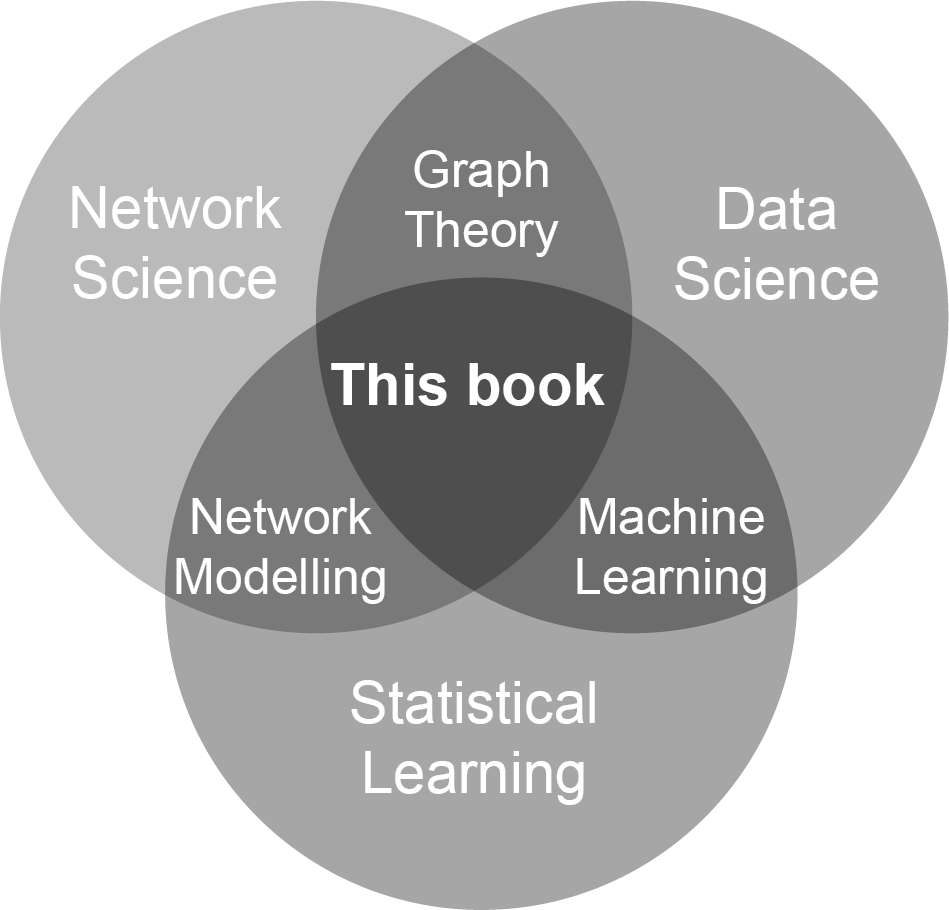
\includegraphics{Images/this_book.png}
    \caption[Venn diagram of network machine learning]{Broadly, we think that the techniques developed and described in this book fall somewhere in the middle of this Venn Diagram.}
    \label{fig:this_book}
\end{figure}

We'll cover the fundamentals of network machine learning, focusing on developing intuition on networks with relevant \texttt{python} tutorials. By the end of this book, you will be able to utilize efficient and easy-to-use tools available for performing analyses on networks. You will also have a whole new range of techniques in your toolbox, such as representations, theory, and algorithms for networks.

We'll show how to do this using production-ready \texttt{python} frameworks:
\begin{enumerate}
    \item \texttt{numpy} \cite{numpy} and \texttt{scipy} \cite{scipy} are used for scientific programming. They give you access to array objects, which are the main way we'll represent networks computationally.
    \item \texttt{scikit-learn} \cite{sklearn} is very easy-to-use, yet it implements many machine learning algorithms efficiently, so it makes a great entry point for downstream analysis of networks.
    \item \texttt{graspologic} \cite{graspologic} and \texttt{networkx} \cite{networkx} are an open-source Python packages which gives you utilities and algorithms for doing analyses on network-valued data.
\end{enumerate}

We focus on developing an intuitive understanding of networks with concrete working examples and a bit of theory. While you can read this book without picking up your laptop, we highly recommend you experiment with the code examples available interspersed throughout the book.

There are many languages and software packages that are extremely useful for network data. When writing this book, we were faced with numerous design choices, and unfortunately it is not feasible to write the entire textbook with tools for every possible language or package for network analysis. There are numerous packages and built-in utilities in \texttt{matlab}, and \texttt{R} has the \texttt{igraph} \cite{csardi2006} package which provides complementary functionality to many of the techniques we discuss herein.

If you are unfamiliar with \texttt{python} but are familiar with another language, we do not think you will find this to be a substantial hurdle (and you might even come out of it with a new programming language skill!). 

\section*{Prerequisites}

Because network science uses a lot of linear algebra, requiring a bit of linear algebra knowledge is unavoidable. We expect you have some familiarity with matrices and the basic operations you can do with them: multiplication, addition, and so on.

If you want to best understand the concepts of this book, we think it would be valuable for you to come in with some background in machine learning. Much of the content will very related to a particular sub-domain of machine learning known as \textit{statistical learning}. This area of research focuses on incorporating statistics with machine learning to better understand and analyze machine learning algorithms. We will assume that you are loosely familiar with probability and statistics (you know what it means for something to be random), but we won't delve too deep into the weeds.

You should also probably have some background in programming -- we'll mainly be using \texttt{python} to build and explore our networks. If you don't have too much of a Python or math background, don't worry -- we'll link some resources to give you a head start.

Another tool we will use, \texttt{jupyter}, is a great tool to have in your toolbox and it's easy to learn. We'll also link some resources for you if you are not familiar with Python's scientific libraries, and we provide a full scientific container pre-loaded with a full programming environment already set up for you in one-click via \texttt{docker} \cite{docker}. 

If you care about what's under the hood, we have appendices which isolate the theoretical underpinnings of the techniques developed herein -- you should have a reasonable understanding of college-level math, such as calculus, linear algebra, probability, and statistics for these sections.

\section*{Roadmap}

This book is organized into four parts.

\begin{itemize}[leftmargin=1cm]
    \item [Part \ref{p:found}] Foundations gives you a brief overview of the kinds of things you'll be doing in this book, and shows you how to solve a network machine learning problem from start to finish. It covers the following topics:
    \begin{itemize}
        \item What a network is and where you can find network data
        \item Many the reasons why we study network data
        \item Examples of ways you could apply network machine learning to your own projects
        \item An overview of the types of problems network machine learning is good at dealing with
        \item Exploring a real network machine learning dataset, to get a broad understanding of what you might be able to learn
    \end{itemize}
    \item [Part \ref{p:rep}] Representations is all about how we can conceptualize networks intuitively, and what we can do with differents ways to represent and conceptualize them. It covers the following topics:
    \begin{itemize}
        \item The various useful properties different types of networks have
        \item Types of network representations and why they're useful
        \item Ways you can represent individual or groups of networks
        \item How to represent networks or groups of networks as tabular data
        \item How to incorporate additional information (attributions) to networks
    \end{itemize}
    \item [Part \ref{p:app}] Applications is about using the representations from Part \ref{p:rep} to explore and exploit your networks for downstream tasks. It covers the following topics:
    \begin{itemize}
        \item Figuring out if communities in your networks are different from each other
        \item Selecting a reasonable model to represent your data
        \item Finding nodes, edges, or communities in your networks that are interesting
        \item Finding time points which are anomalies in a network that is evolving over time
        \item What to do when you have new data after you've already trained a network model
        \item How hypothesis testing works with networks
        \item Figuring out which nodes are the most similar in a pair of networks
    \end{itemize}
    \item [Part \ref{p:next}] Next Steps discusses concepts that don't directly tie into the story we hope to tell, but we believe they are extremely important ideas to be aware of and introduced to, and we believe that we can help situate you with these concepts so that you can learn more about them on your own. They are:
    \begin{itemize}
        \item Graph neural networks
        \item Diffusion methods for networks
        \item Network sparsity
        \item a path forward for you to continue your journey with network machine learning
    \end{itemize}
\end{itemize}
The appendices provide an brief overview of what we consider to be higher-level concepts. In the interest of keeping this book approachable, the main content of the work has, admittedly, left out many technical details and considerations that might be very useful for readers farther along in their journey through math and statistics. You will find these details in here.

\section*{Other resources}

Many resources exist which will help you greatly with the content of this book. 

If you don't have any background in machine learning quite yet, our favorite starting point is Aur\'elian G\'eron's excellent work \cite{Geron2017Mar}. We would recommend starting with an introduction to machine learning \textit{prior to} focusing on this book, because many of the concepts and ideas of this text will make more sense coming in with a machine learning background, however brief. The core ideas you should remember are the types of machine learning problems, some of the more common algorithms and techniques for machine learning (\texttt{K-Means}, testing, and validation each come up a few times), and the basic data structures used for machine learning.

To our knowledge, there are no other books which explicitly focus on network machine learning for single and multiple network problems just yet, and moreover, there are also none that do this with a programming component. If you want some more exposure to networks in general, we would recommend the following works:
\begin{enumerate}
    \item ``Network Science'' \cite{Barabasi2016Aug}, which provides an approachable and well-grounded introduction to network science.
    \item ``Networks'' \cite{Newman2018Sep}, which provides an expansive glance at the mathematics of networks and network models.
    \item ``Python for Graph and Network Analysis''\cite{AlTaie2017}, which presents network analysis techniques in \texttt{python}.
    \item ``Network Analysis'' \cite{Brandes2005}, which focuses on the development of the network data structure and summary statistics for networks.
    \item ``A User's Guide to Network Analysis in \texttt{R}'' \cite{Luke2015}, which provides a hands-on introduction to network analytics techniques in the \texttt{R} programming language.
    \item ``Statistical Analysis of Network Data'' \cite{Kolaczyk2009}, which presents statistical models and methods for network science.
\end{enumerate}

If you haven't seen linear algebra in a while, we would recommend that you start with the book ``Numerical Linear Algebra'' \citep{Trefethen1997}, by Trefethan and Bau. The first 4 lectures succinctly and effectively summarize all of the properties of matrices that we will need for this book. You will also want to have some exposure to basic statistics and statistical inference; if you can read and understand the wikipedia summaries (at the top of the page) on ``random variable'', ``normal distribution'', and ``bernoulli distribution'', we think that you will have plenty of statistical background to make it through this book. 

If you are looking for a more comprehensive overview, a good introduction is \citep{Casella2001Jun} by Casella and Berger, and a good refresher is \cite{Bickel2006May} by Bickel and Doksum. It may also be helpful to be explicitly introduced to statistical learning; our favorite is \citep{James2021Jul}, by Jones, Witten, Hastie, and Tibshirani.

\begin{comment}
\section*{Material we won't cover}

The network data structure has quickly become a go-to across many domains of science and industry. One application of networks is particularly appealing: networks can be used to succinctly conceptualize and visualize underlying relationships that exist outside of just network-valued data. One of the most prominent applications of this concept uses machinery known as a \textit{Directed Acyclic Graph} (or DAG) to conceptualize the ``flow'' between different elements in an underlying system. Since graph is just another word for network, this concept is inherently rooted in networks. 
\end{comment}

\section*{Conventions used in this book}

The following conventions are used in this book:

\begin{itemize}
    \item \emph{Italics}: indicates emphasis behind a term or exclamation. Also often used when terms have not yet been defined, but a definition is upcoming.
    \item \textbf{Bold face}: indicates a definition for a term or concept.
    \item \texttt{Unicode block}: used to indicate the name of an algorithm, function names, package names, programmatic text elements, and related concepts.
\end{itemize}

\begin{floatingbox}[h]
\caption{Remarks}
Used to indicate ideas that are directly relevant or supplementary to the content of the book, but are not essential for understanding the main concepts of a section or paragraph.
\label{fb}
\end{floatingbox}

\subsection*{Code examples}

The entirety of this book has been compiled using \texttt{jupyter} notebooks, integrated through the \texttt{jupyter-book} framework. The book is currently hosted on github at \texttt{github.com/neurodata/graph-stats-book}, and the build log for the text can be found at \texttt{github.com/neurodata/graph-stats-book/actions}. You can find every section notebook, and every command which was used to prepare the environment in which the corresponding textbook pages were executed, using those two links. 

All of the code used to prepare simulations or algorithms are contained within this book. For example, a python code block, and its corresponding expected output, will look like this:
\begin{lstlisting}[style=python]
def howdy_world():
    # A function to print informative text.
    print("Howdy world!")
howdy_world()
# Hello world!
\end{lstlisting}

When discussing how to set up your initial environment, we'll occassionally demonstrate \texttt{bash} commands that should be used directly from a terminal session. If you have Mac or Linux operating systems, you can get to these directly using the \texttt{terminal} utility, which should come with your computer pre-installed. If you have a Window's operating system, things are a little bit more complicated, but we have some instructions for you in Chapter \ref{sec:ch2}.

Bash code blocks can be identified by code blocks that start with a \texttt{\$}, and will look like this:

\begin{lstlisting}[style=bash]
$ echo "these is a bash demo"
this is a bash demo
\end{lstlisting}


Throughout this book, we will focus a lot of attention on visualizations and plotting, the code for which can quickly become extremely cumbersome. For all programmatically generated figures, we will show you how to generate the figure first with explicit code, and then will assume that you will be able to generate these plots on your own later on. That said, the code to recreate all plots can be found online, at \texttt{docs.neurodata.io/graph-stats-book}. Simply page to the appropriate section of the book, and identify the appropriate plot that you want to recreate. 

\paragraph*{A disclaimer about the impact of randomness}

In most of our examples, we are going to use simulations and approaches which inherently involve randomness. Running the same piece of code twice, you will probably not get the same result. The reason that we do this is two-fold:
\begin{enumerate}
    \item Using simulations will allow you to modify, manipulate, and ``play with'' the algorithms and approaches so that you can build insight. We are hoping that this book will be ``hands-on'' on your end: we \textit{want} you to try to vary around the networks that you are using as you go, so that you can challenge your intuition and use what you observe to solidify or modify your intuition accordingly. This has the caveat that every simulation run will produce a slightly different answer, and your plots might not match up with the plots that we produce exactly.
    \item Many algorithms that deal with networks use some hints of randomness to achieve solutions which are either faster or numerically superior to solutions that do not use randomness. In getting you accustomed to working with network data using approaches that are relevant in the field, we cannot ignore these techniques. Running the same algorithm on the same network twice might produce slightly different results.
\end{enumerate}

That said, the broad implications of each code segment on your machine should produce a similar (but perhaps not identical) conclusion to what we reach in our plots. If a particular technique will be problematic, we will hard-code 


\subsection*{Using code examples, citing the book, and reaching out with feedback}

This book is intended to teach you how to develop code for network machine learning. In general, we are providing this code for you: it is intended that you will borrow and repurpose the code and techniques we describe in your programs and documentation. If you are using a few brief snippets from our book for your work, feel free with proper attribution to our citation (below). If you want to write a program that borrows some code, feel free without permission. If you intend to sell or financially profit directly from code we provide in this book, you need to request permission.

To cite our textbook, you can use the following citation: 

Eric W. Bridgeford, Alexander R. Loftus, and Joshua T. Vogelstein. \emph{Hands-on Network Machine Learning with Scikit-Learn and Graspologic}. Cambridge University Press.

To request permissions, provide us with feedback about our in-progress draft, or even just to say hi and let us know what network machine learning concepts you want to see us discuss, feel free to reach out to the authors directly. You can reach out to us at \texttt{ericwb95@gmail.com}.

\subsection*{About the authors}

\textbf{Eric W. Bridgeford} is a Ph.D. student in the Department of Biostatistics at Johns Hopkins University. Eric’s background includes Computer Science and Biomedical Engineering, and he is an avid contributor of packages to \texttt{CRAN} and \texttt{pypi} for nonparametric hypothesis testing. Eric studies general approaches for statistical inference in network data, with applications to problems with network estimation in MRI connectomics data, including replicability and batch effects. He was a core contributor to the backbone of the \texttt{graspologic} package.

\noindent\textbf{Alex R. Loftus} is a master’s student at Johns Hopkins University in the Department of Biomedical Engineering, with an undergraduate degree in neuroscience. He has worked on implementing network spectral embedding and clustering algorithms in Python, and helped develop an MRI pipeline to produce brain networks from diffusion MRI data.

\noindent\textbf{Joshua T. Vogelstein, Ph.D.} is an Associate Professor in the Department of Biomedical Engineering at Johns Hopkins University, with joint appointments in Applied Mathematics and Statistics, Computer Science, Electrical and Computer Engineering, Neuroscience, and Biostatistics. His research focuses on the statistics of networks in brain science (connectomes). His lab and collaborators have developed many leading computational algorithms and libraries to perform statistical analysis on networks.

\paragraph{Section Contributors}

\textbf{Jes{\'u}s Daniel Arroyo, Ph.D.} is an Assistant Professor in the Department of Statistics at Texas A\&M University. He focuses on the theoretical underpinnings of statistical network analysis, machine learning, and high-dimensional data analysis, including topics such as spectral graph inference, dimensionality reduction, convex optimization, and graph matching. Jes\'us tends to focus on the applications of his work to neuroimaging data in statistical connectomics.

\noindent\textbf{Ali Saad-Eldin} is a software engineer at Amazon. As a masters student at Johns Hopkins University in Applied Mathematics and Statistics, Ali focused his attention on optimization techniques for solving problems in graph analysis. He was a core contributor to the \texttt{graspologic} package and developed the submodule for graph matching. Ali helped to write the section on graph matching.

\noindent\textbf{Sambit Panda} is a Ph.D. student at Johns Hopkins University in the Department of Biomedical Engineering. Sambit's work focuses on nonparametric hypothesis testing for large datasets, with applications in neuroimaging. He was a core contributor to the `hyppo` package, which is a python framework for hypothesis testing. Sambit helped to write the section on two-sample hypothesis testing.

\noindent\textbf{Jason Yim} is a Ph.D. student at Massachusetts Institute of Technology in the Department of Electrical Engineering and Computer Science (EECS), where he develops generative models for de-novo protein design. Prior to starting his PhD, Jason focused on the application of neural networks to protein folding and macular degeneration with DeepMind, a company focused on artificial intelligence that was acquired by Google in 2014. Jason helped to write the section on graph neural networks.

\section*{Acknowledgements}

First and foremost, we want to acknowledge all of the monumental contributions to science that made this book possible. We would not have been capable of producing this work without the work of our many collaborators and the greater scientific community. Academic-focused books are produced as much by the authors as they are by the many wonderful contributors that developed the works that comprise this book. Throughout each chapter of this book, we'll list out the key papers in the bibliography that you can check out that led to the insights that go into each section. You can use these papers in conjunction with the appendix (where applicable) to find more detailed and technical descriptions of the particular algorithms and techniques we describe in this book. 

Finally, we want to offer a big thanks to everybody who has been reading the book as we write. So far, this list includes our wonderful editor Lauren Cowles, as well as Dax Pryce, Ross Lawrence, Geoff Loftus, Alexandra McCoy, Olivia Taylor, and Peter Brown. Writing a large textbook is not easy, and we truly appreciate all of the gracious feedback that we have been offered throughout the writing stages as we refine this book.

\bibliographystyle{vancouver}
\bibliography{references}
% notation.tex
% 2011/02/03, v1.10

\chapter*{Terminology}

In this section, we outline some background terminology which will come up repeatedly throughout the book. This section attempts to standardize some background material that we think is useful going in.

\paragraph{Mathematical concepts}

\begin{tabular}{p{2cm} | p{4.5cm} | p{4cm}}
\hline
    Symbol & Definition & Description/Example \\
    \hline
     $x$ & A scalar number & $x = 5$   \\
     $\vec x$ & A column vector & $\vec x = \begin{bmatrix}5 \\ 2 \\ 6\end{bmatrix}$ \\
     $x_i$ & the $i^{th}$ element of a column vector & $x_2 = 2$ \\
     $\mathcal X$ & A set & $\mathcal I = \{1, 2\}$\\
     $\sum_{i \in \mathcal N} x_i$ & A sum indexed by a set $\mathcal N$ & $\sum_{i \in \mathcal I} x_i\equiv \sum_{i = 1}^2 x_i = 7$ \\
     $\prod_{i \in \mathcal N}x_i$ & A product indexed by a set $\mathcal N$ & $\prod_{i \in \mathcal I} x_i \equiv \prod_{i = 1}^2 x_i = 10$ \\
     $Y$ & A matrix & $Y = \begin{bmatrix}1 & 2 \\ 3 & 4\end{bmatrix}$ \\
     $y_{ij}$ & The $(i, j)^{th}$ element of a matrix & $y_{22} = 4$ \\
     \hline
\end{tabular}


\paragraph{Mathematical operations}

\begin{tabular}{p{2cm} | p{4.5cm} | p{4cm}}
\hline
    Operation & Name & Definition \\
    \hline
     $\vec x^\top \vec y$ & The Euclidean inner product & $\sum_{i = 1}^n x_i y_i$ \\
     $C = AB$ & Matrix multiplication & $c_{ij} = \sum_{k = 1}^n a_{ik} b_{kl}$ \\
     $||\vec x||_k$ & The $k$-norm of $\vec x$ & $\left(\sum_{i = 1}^n |x_i|^k\right)^{\frac{1}{k}}$ \\
     $||\vec x - \vec y||_2$ & The Euclidean distance between $\vec x$ and $\vec y$ & $\sqrt{\sum_{i = 1}^n (x_i - y_i)^2}$ \\
     $||X||_F$ & The Frobenius norm of $X$ & $\sqrt{\sum_{i = 1}^r \sum_{j = 1}^c x_{ij}^2}$ \\
     \hline
\end{tabular}

\paragraph{Probability and statistics concepts}

For most of this work, we will assume a fairly limited background in probability and statistics. You should have a general concept of randomness, and know what a random variable is (for example, a Normal or Gaussian random variable, or a Bernoulli ``coin flip'' random variable). If you haven't seen these in a while, see if you can get through the summaries of the pages for ``random variable'', ``normal distribution'', and ``bernoulli distribution'' on wikipedia. We don't think that you will need any of the detailed technical knowledge on the pages beyond having intuition for what these concepts are. The notation that we will use in this book is:

\begin{tabular}{p{2cm} | p{4cm} | p{4cm}}
\hline
    Symbol & Explanation & Example \\
    \hline
    $\mathbf x$ & A random variable & $\mathbf x$ takes the value $0$ or $1$ with probability $0.5$\\
    $\vec{\mathbf y}$ & A random vector & $\vec{\mathbf y} = \begin{bmatrix}
         {\mathbf y}_1 \\ {\mathbf y}_2
     \end{bmatrix}$ \\
    $\mathbf Z$ & A random matrix & $\mathbf Z = \begin{bmatrix}\mathbf z_{11} & \mathbf z_{12} \\ \mathbf z_{21} & \mathbf z_{22}\end{bmatrix}$ \\
    $Pr(A)$ & Probability that an event $A$ happens & $Pr(\mathbf x = 1) = 0.5$ \\
    $Bern(p)$ & The Bernoulli distribution with probability $p$ & If $\mathbf x$ is a $Bern(p)$ random variable, then $Pr(\mathbf x = 1) = p$, and $Pr(\mathbf x = 0) = 1-p$ \\
    \hline
\end{tabular}


\bibliographystyle{vancouver}
\bibliography{references}

\endinput

\mainmatter
\part{Foundations}
\label{p:found}
\chapter{The Network Machine Learning Landscape}
\label{sec:ch1}

In this section, we'll cover the basics of the network machine learning landscape. We learn a lot of high level elements about networks, and introduce some of the basic terminology for network data. This will give you an understanding of the basics of the network data structure, which will make Chapter \ref{sec:ch4} more digestible when we formally introduce network data structures and how you can manipulate them. 

We take a look at the different types of problems you might come across in network machine learning, and how network data fits into the types of problems you want to adress. Then, we'll see how a particular branch of mathematics,  \emph{statistics}, fits into the machine learning landscape. This chapter will be very high level, but will allow you to see how the pieces of the book fit together in the grand scheme of things. 

Here are some basic questions that we will approach in these next sections:
\begin{enumerate}
    \item How do networks fit into the world of machine learning, and why are they important?
    \item What does it mean to learn from a network, and what kinds of things would you be trying to learn?
    \item How can we use network-valued data to understand the world better?
\end{enumerate}

Having a good understanding of the high level will help you see how the lower level parts fit together in terms of your ultimate goal of applying network machine learning to new and exciting problems in your work. 

\newpage 

\section{What is network machine learning?}
\label{sec:ch1:whatis}

If you are reading this book, you probably have some idea what the term ``machine learning'' means. According to wikipedia \cite{wikiML}, machine learning is a field of inquiry devoted to understanding and building methods that {learn}; that is, methods that leverage data to improve performance on some set of tasks.

For instance, if you have an image and you are a photo editor working in pattern recognition, you might want to learn how you can automatically segment a person so that you can blur the background, (see Figure \ref{fig:ch1:ml-ex}. ) If you are doing natural language processing, you might want to learn how identify the unique instruments in the song on an audio track. If you are a scientist, you might want to learn how a lobster's size correlates with its age so that you can predict lobsters' average age.  What unites these examples is that in all of them you are using data,  to learn something so that you can accomplish some task. Machine learning has grown enormously over the past few decades, and the use-cases of machine learning are rapidly coming to pervade modern life.

\begin{figure}[h]
    \centering
    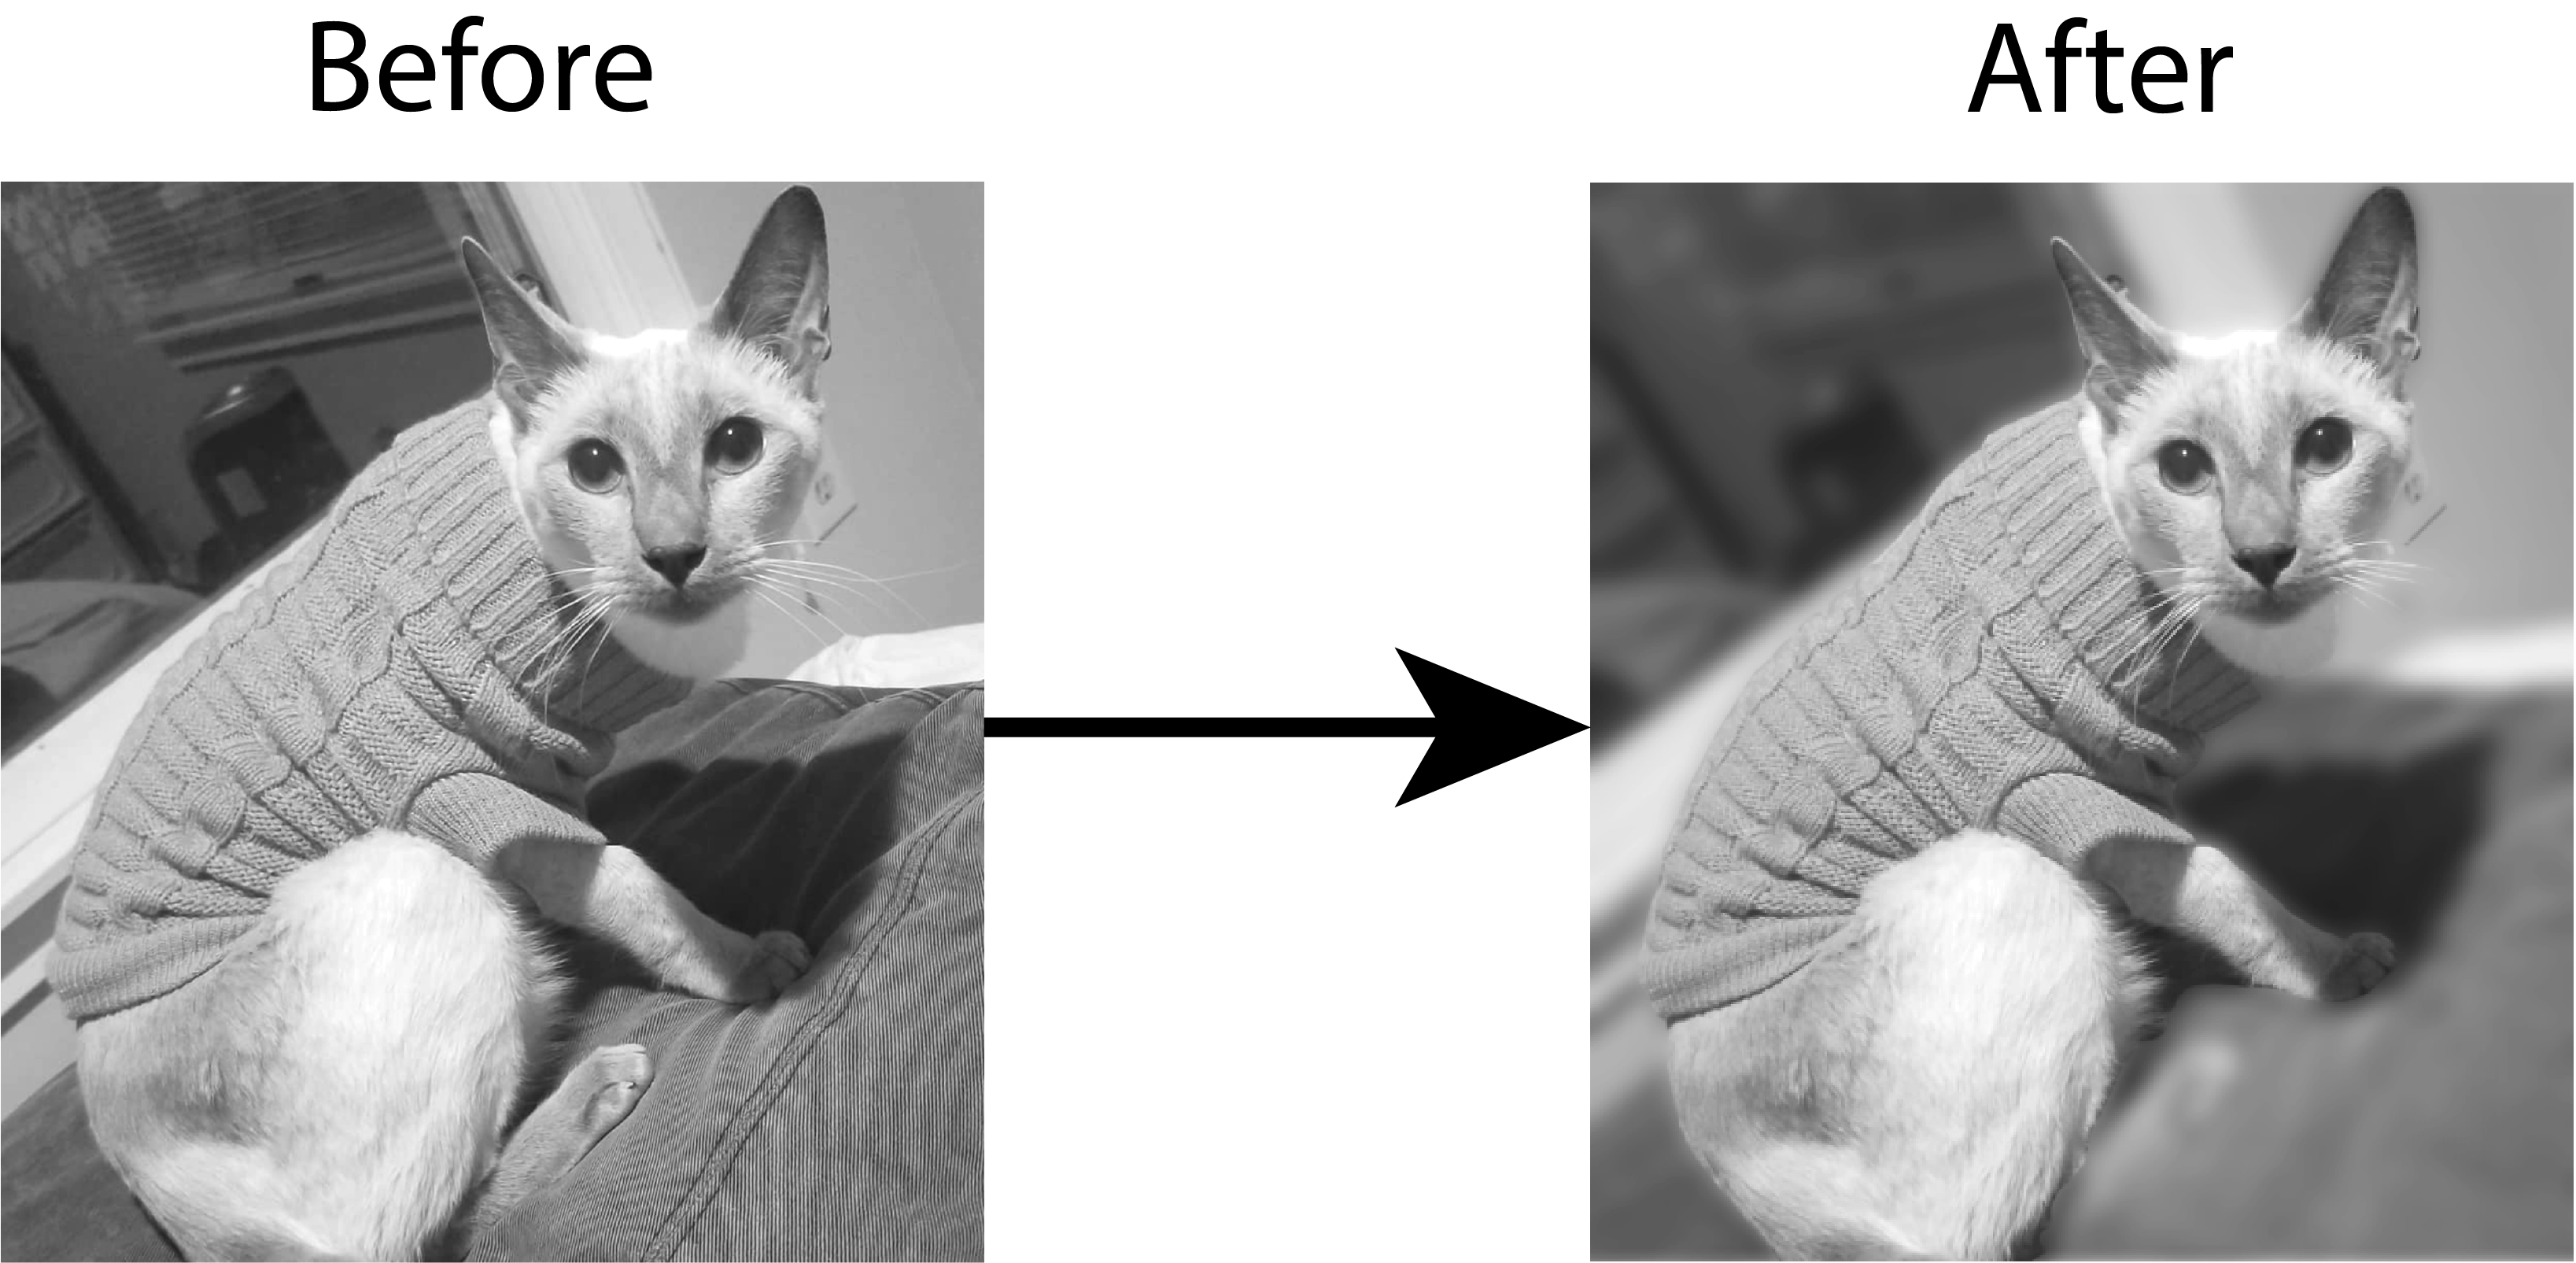
\includegraphics[width=\linewidth]{foundations/ch1/Images/cboy.png}
    \caption[Machine learning task]{Learning how to segment an image to blur the background. A machine learning system is trained using numerous images with the foreground segmented out. This trained system is then used to segment out the foreground on new images, and then the background is blurred.}
    \label{fig:ch1:ml-ex}
\end{figure}


\subsection{Traditional machine learning leverages tabular data structures}

In traditional machine learning, data follows what is called a \textit{tabular} format. This means that the data are arranged in a table or an array, where each row represents a single observation. We recommend you check out the Pandas tutorial on tabular data \cite{pandastut}. 

Conveniently, a lot of modern developments in machine learning apply directly to tabular data. This means that, with some amount of effort, one can take techniques developed in one domain of machine learning, and readily modify or apply them to problems in another domain of machine learning, without needing to {reinvent the wheel}. By this we mean that you can focus your effort on your problem, and borrow techniques developed for related problems, without having to start from scratch every time. For example, if you had a tabular dataset where each row represented a lobster with two columns representing the length and sex of the lobster, you might try to learn how these columns can be used to predict the lobster's claw size. You could do this using an extremely general approach, by simply producing a line of best fit for the claw size depending on which biological sex a lobster is. 

In Figure \ref{fig:ch1:tabular-dat}, we look at how tabular data fits into a machine learning system. This example comprises a basic classification task, in which each observation is either blue or orange. Some of the data (the {training set}, circles) is used to train a machine learning algorithm ({learning}, the transparent blue and orange voronoi cells), and the remainder of the data is used to test the trained algorithm on new data ({evaluating} on the squares using the voronoi cells learned). The trained model can then be further refined ({updated}), or deployed for your intended use-case.

\begin{figure}[h]
    \centering
    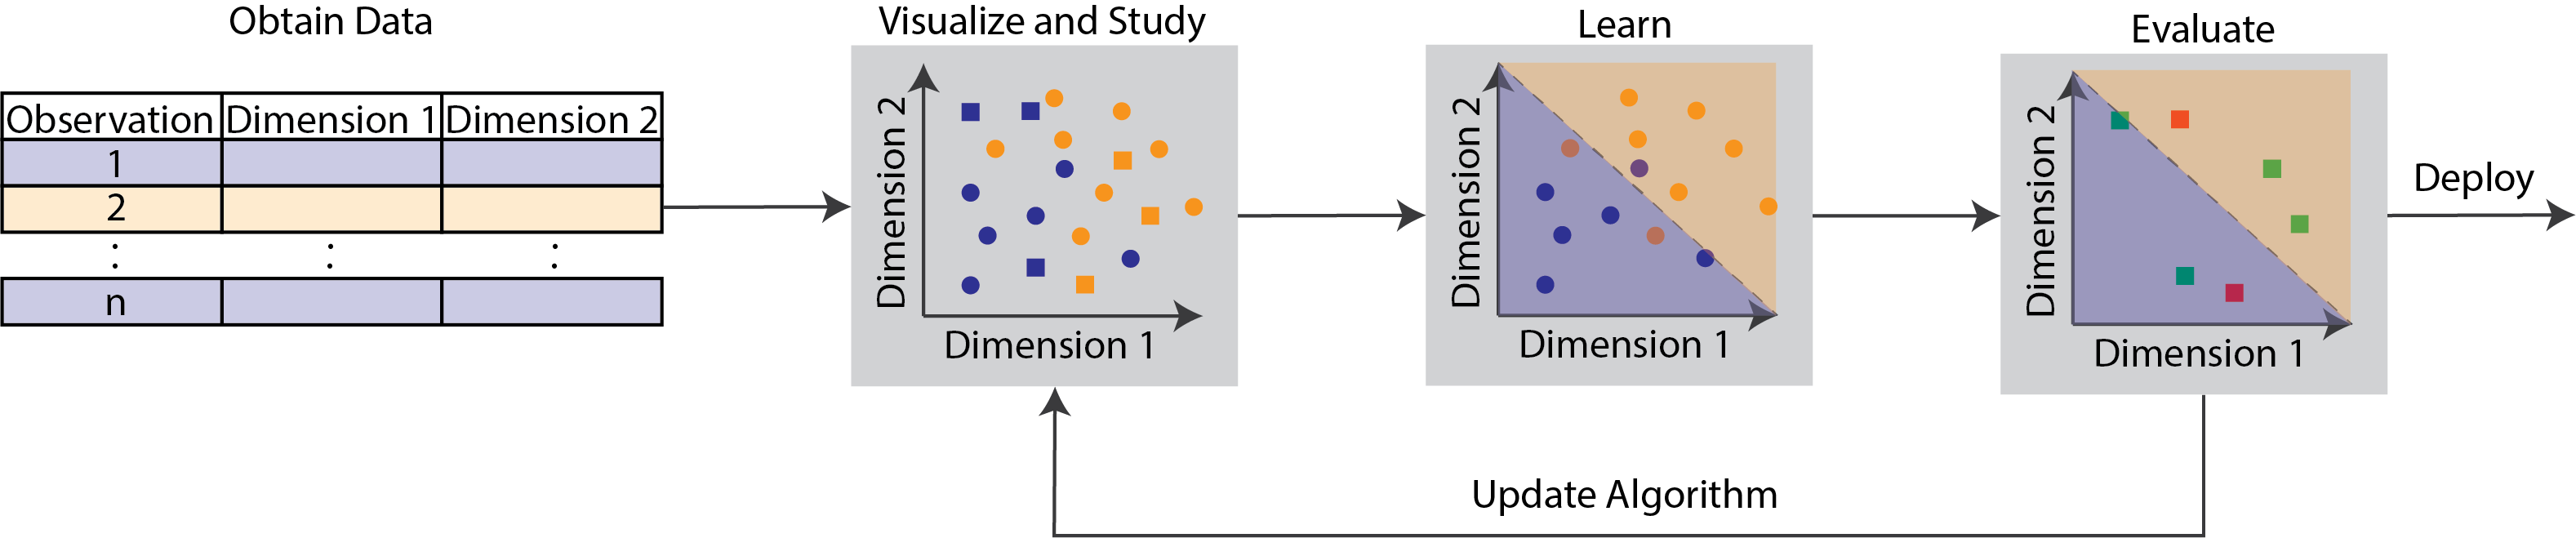
\includegraphics[width=\linewidth]{foundations/ch1/Images/ml_ex.png}
    \caption[Machine learning system]{Machine learning systems start by obtaining inputs as tabular data, where the rows are observations and the columns are features, i.e.  \textit{dimensions} of each observation.}
    \label{fig:ch1:tabular-dat}
\end{figure}

\subsection{What is a network?}

So, what does this have to do with networks? As it turns out, in the 21st century, networks are all around us. When most people think of a ``network'', they often have some vague image in their head of the internet, or of cell phone towers transmitting data, or of some other technical system. But networks have a specific definition in the world of machine learning and data science. The most direct example can easily be explained through the recent rise in social media over the last decade. In a network, your data follows a prescribed pattern: a group of items (say, people on the social network) are interconnected to one another through clearly defined relationships (say which people are friends with one another in the network). 

In other places, you might hear networks referred to as ``graphs'', and the field studying them as ``graph theory''. We try to avoid this terminology in this book, since it's easy to confuse a graph and a plot with an $x$/$y$ coordinate axis. We'll stick to the term ``network'' throughout this book when possible. There might be times when we choose to use the word ``graph'', since the name of some algorithm or tool we're showing you uses it, but just remember that they mean the same thing.

\begin{figure}[h]
    \centering
    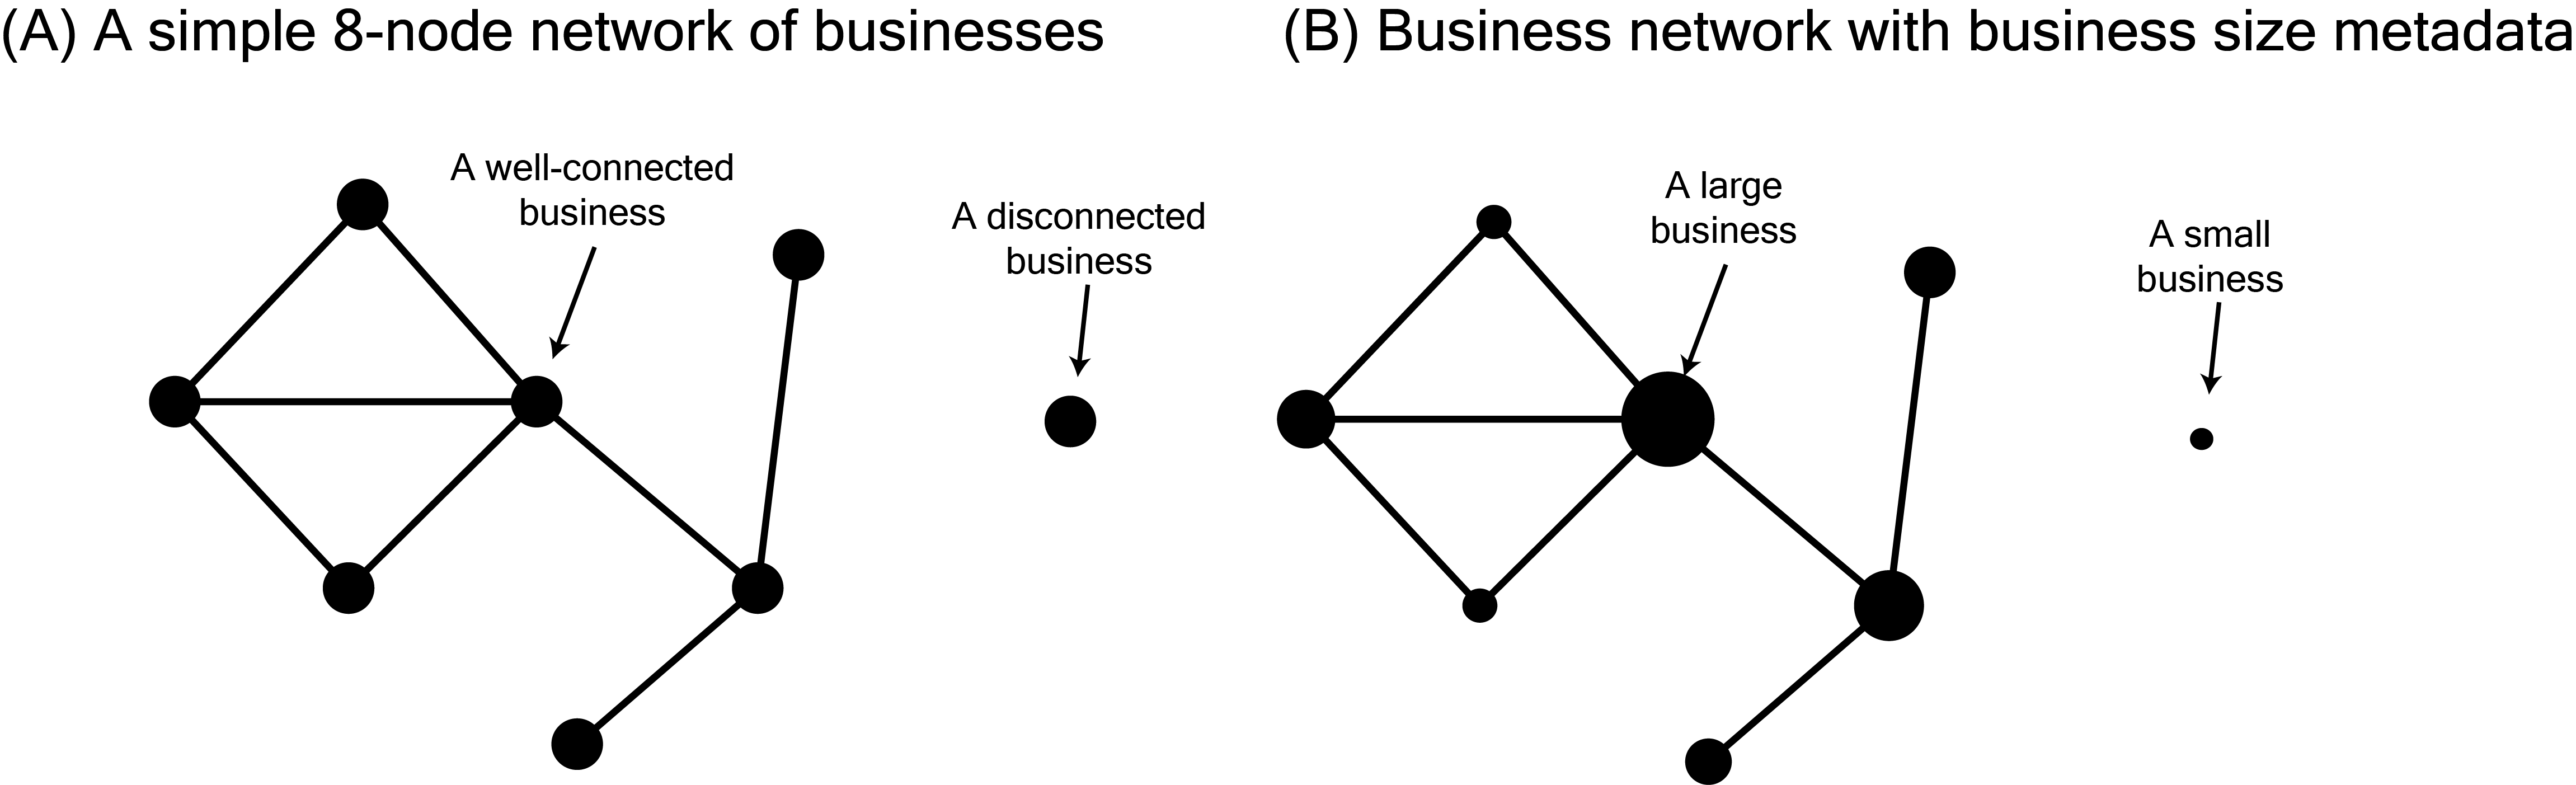
\includegraphics[width=\linewidth]{foundations/ch1/Images/simp_net.png}
    \caption[Simple network example]{\textbf{(A)} indicates a simple network, where nodes are businesses, and edges exist if a given pair of businesses transact with one another. \textbf{(B)} indicates the same simple network, but each node also has a piece of information attached to it, the number of employees (indicated by the node size).}
    \label{fig:ch1:simplenet}
\end{figure}

Let's get more specific about what we mean. Each object in your network is called a \textit{node}, or a vertex (for consistency we'll stick to "node" in this book). A connection between two nodes is called an \textit{edge}. Below you can see a visualization of a simple network with 8 nodes. As you can see, some nodes are well-connected with other nodes -- for example, the node in the center, has edges to five other nodes -- and you can also have nodes which aren't connected to anything, like the lonely extra node without any edges. This is illustrated in Figure \ref{fig:ch1:simplenet}(A).

Networks might also contain extra information. Each node might have a set of features attached to it: extra information that comes in the form of a table. Say the network we just made represents business transactions. Assume that there are eight companies, one corresponding to each node, and there is an edge if one company has sold something to another.

Then, we might also have information about the company size. If the company is larger, you might assume that it'll tend to have had more business transactions with the other companies. The network, in this case, includes the company size information. This is illustrated in Figure \ref{fig:ch1:simplenet}(B).

\subsection{Why do we study networks?}
\label{sec:ch1:howstudy}

If you think about it, you can see networks everywhere. The objects could be people, and the edges could be friendships. Or the objects could be computers, and the relationship could be the information they send to each other. if you're working in air traffic control, you'd have flight networks where the edges are flights from City A to City B; or if you're an epidemiologist studying disease, you could create an infection network. Neuroscientists explore brain networks, consisting of neurons and their relationships with each other, and computer scientists often use neural networks, which have become pillars of machine learning.

Networks can even be used to visualize ideas: in a Bayesian network, nodes represent a set of variables and the edges represent their conditional dependencies. In a correlation network, nodes represent variables, and the edges represent the correlation between those variables. You can have ecological networks, electrical networks, gene networks, or you could visualize your team's workflow with a network.

Even the way we think can be thought of as a network. Visualize a concept or object in your head. Maybe you could think about the food you had for breakfast this morning, or the city you live in. Now, think about the connections between those concepts and others. Maybe you had eggs and toast for breakfast. Eggs and toast are connected with a multitude of other concepts in your head: forks and silverware, kitchens, hunger, protein, carbohydrates, your morning routine, chickens, wheat, other breakfast foods, and innumerable other things. What you're doing right now is exploring a small part of the massive semantic network that exists in your head.

Network machine learning is a relatively new field. The vast majority of it has been invented (or discovered) after the year 2000, and many fundamental proofs have only been published recently. 

For the business-minded readers out there, this is an incredible time to learn about networks. Graph neural networks (GNNs) are becoming increasingly popular as deep learning and neural networks proliferate. This book provides the basic foundational concepts and intuition required to understand how, when, and why GNNs, or any other network machine learning tool, work.

Real-life applications also follow a general trend. It begins with academics spending a lot of time, usually 10-20 years, publishing proof-of-concept papers, discussing possible approaches to solve problems, and developing fundamental tools (usually informally, with somewhat messy code that exists in jupyter notebooks). Then, as the field of research starts maturing, companies and industry people start noticing these new academic tools. They find ways to apply them to make their product or service better, and they develop easy-to-use packages like \texttt{scikit-learn} to make these academic tools mainstream. Network machine learning is at a tipping point right now: its academic foundations have been built up over the past 10-20 years, and the tools for building and working with networks are now starting to move from academia to industry. Congratulations: you could get in early for a wave of application-focused network machine learning tools!


\subsubsection{Why do we need special machine learning approaches for networks?}

As you will learn throughout this book, the problem you run into is that networks mostly exist not in their most naive form, tabular data, but instead in network-valued data. This means, unfortunately, that all those techniques that were developed over decades for tabular data cannot, natively, be used for network-valued data. However, as we will see, we can take various approaches to {adapt} networks to a more traditional format, including tabular structures using network representations. Once we adapt these networks  to more traditional structures, we can then apply techniques from other domains of machine learning to learn about our networks. In Figure \ref{fig:ch1:nml-high-level}, we see how network machine learning functions at a high level. Loosely, \textit{network machine learning} is machine learning for network-valued data (data which is a {network}, not a {tabular structure}). 

\begin{figure}
    \centering
    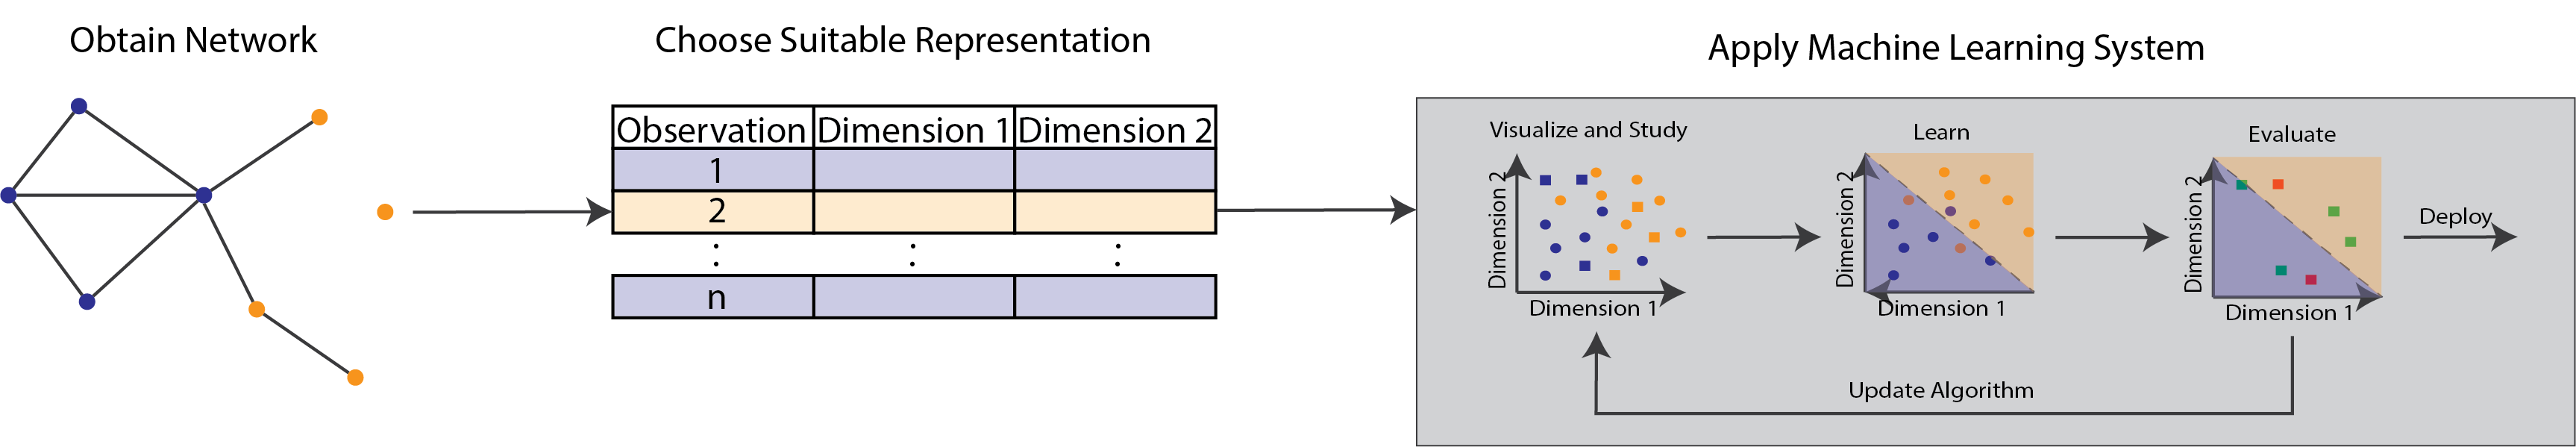
\includegraphics[width=\linewidth]{foundations/ch1/Images/nml-high-level.png}
    \caption[Network machine learning]{In network machine learning, we start by obtaining a network. The first step in network machine learning is to select a suitable representation for the network, which depends on the type of questions you are asking. Using this representation, you apply a machine learning system which is suited appropriately for the type of task that you have. As the set of questions one might have about network data may differ from a typical tabular dataset, the manner in which these techniques are applied may need to be tuned for the question of interest.}
    \label{fig:ch1:nml-high-level}
\end{figure}



Let's get started!

\newpage
% \section{Why do we study networks?}
\label{sec:ch1:howstudy}

When you start thinking, you start seeing networks everywhere. The objects could be people, and the edges could be friendships. Or they could be computers, and the relationship could be the information they send to each other. You'd have airflight networks if you're working in air traffic control, where the edges are flights from city A to B; or if you're an epidemiologist studying disease, you could create an infection network. Neuroscientists can explore brain networks, which tell them about neurons and their relationships with each other, and computer scientists often use neural networks, which have become pillars in machine learning.

Networks can even be used to visualize ideas: in a Bayesian network, your nodes represent a set of variables and the relationship between them is their conditional dependencies. In a correlation network, your nodes represent variables, and the edges represent the correlation between those variables. You can have ecological networks, electrical networks, gene networks, and you could visualize your team's workflow with a network.

Even the way we think can be thought of as a network. Visualize a concept or object in your head. Maybe you could think about the food you had for breakfast this morning, or the city you live in. Now, think about the connections between those concepts and others. Maybe you had eggs and toast for breakfast. Eggs and toast are connected with a multitude of other concepts in your head: forks and silverware, kitchens, hunger, protein, carbohydrates, your morning routine, chickens, wheat, other breakfast foods, and an innumerable amount of other things. What you're doing right now is exploring a small part of the massive semantic network that lives in your head.

Network machine learning is a relatively new field. The vast majority of it has been invented (or discovered) after the year 2000, and many fundamental proofs have only been published recently. 

For the business-minded folks out there, this is an incredible time to learn about networks. Graph neural networks (GNNs) are becoming increasingly popular as deep learning and neural networks explode. This book provides the basic foundational concepts and intuition required to understand how, when, and why GNNs, or any other network machine learning tool, work.

Real-life applications also follow a general trend. You'll see academia spend a lot of time, usually 10-20 years, publishing proof-of-concept papers, discussing possible approaches to solve problems, and developing fundamental tools (usually informally, with somewhat messy code that exists in jupyter notebooks). Then, as the field of research starts maturing, companies and industry people start noticing these new academic tools. They find ways to apply them to make their product or service better, and easy-to-use packages like scikit-learn are developed to make these academic tools mainstream. Network machine learning is at a tipping point right now: its academic foundations have been built up over the past 10-20 years, and the tools for building and working with networks are now starting to move from academia to industry. Congratulations: you could get in early for a wave of application-focused network machine learning tools!

\section{Types of network machine learning problems}
\label{sec:ch1:types}


There are many different types of network machine learning systems. We tend to broadly group them into the following categories:
\begin{itemize}
\item whether or not they involve one or multiple networks (single or multiple network learning systems),
\item whether or not they require additional information in the form of network attributes (attributed or non-attributed network learning systems),
\item whether they ask questions about an edge, a node, a group of edges/nodes, or about the network itself, and
\item whether or not the approach can be used in isolation from a statistical model (non-model based or model-based network learning systems).

\end{itemize}

To learn about these criteria, we'll use a few running examples:

\begin{floatingbox}[h]\caption{Brain networks for musicians and non-musicians}
\label{box:ch1:brainnet}
You have brain networks that were acquired from a large group of people. The nodes of this network represent areas of the brain, and the edges represent whether a pair of brain areas can communicate using neurons. Neurons are cells in the brain that receive sensory input from the environment, and work together to transform the sensory input into usable outputs (thoughts, actions, behaviors, etc.) Each brain network is from a person who we know is either a non-musician or a musician.
\end{floatingbox}

\begin{floatingbox}[h]\caption{A pair of social networks for students at a school}
\label{box:ch1:social}
In this network, the nodes represent students who attend one of two schools. Edges represent whether the students are connected on a social media site. We have networks collected from two social media sites, Facebook and Twitter.
\end{floatingbox}

\subsection{Single vs multiple network learning systems}

\subsubsection{Single network learning systems}

In many cases of network learning, you only actually have a single sample: the network itself. A \textit{single network learning system} is a system in which insight is derived from a single network, that is one collection of nodes and edges. In a single network learning system, you only have one sample: the network itself. In a traditional machine learning framework, having a single sample is disastrous: you canot derive insight with one sample in a traditional machine learning framework, because a question cannot be addressed using only one data point. This is an extreme case of the small sample problem. As an example, if you wanted to determine the degree to which cloud cover predicted whether or not it was raining, and you only had one day's worth of data, you would not be able to learn anything, because your answer would totally be determined by whether or not it was cloudy on that particular day and whether or not it was raining on that particular day.

On the other hand, in network learning, a single sample is far from disastrous. While we only have one network, that one network is defined by a collection of nodes and edges. For this to be meaningful, there must be multiple nodes and edges in the first place! While you might only have one network, you can still learn about relationships that exist among the nodes, edges, or both. The caveat is that the conclusions you reach from your network might be limited to the specific network you are studying, or a rather limited sample population, but often that’s not much of a problem.


Most of the strategies in this book address single network learning systems.


\subsubsection{Multiple network learning systems}

A \textit{multiple network learning system} is a system in which insight is derived from multiple networks, wherein you have multiple collections of nodes and edges. Unlike a single network learning system in which you can only obtain conclusions on the basis of characteristics of that particular network itself, in a multiple network learning system, you can obtain insights {both} within and across the networks.


In the brain networks from Example \ref{box:ch1:brainnet}, you can derive insights to describe the commonalities among the brain networks of non-musicians along with the commonalities among the brains of musicians, and then compare them to look for differences between the brain networks of non-musicians and musicians.


Some strategies which employ multiple network learning systems are:
\begin{itemize}
\item multiple network representation learning in Section \ref{sec:ch6:multinet},
\item anomaly detection in Section \ref{sec:ch9:anomaly}, and
\item signal subnetworks in Section \ref{sec:ch9:ssn_incoherent}.
\end{itemize}

Note that these these categories are not mutually exclusive, and a network machine learning system will pull elements from several of the different categories simultaneously. For instance, you might have a machine learning system that is a single network, node-attributed, non-model-based machine learning system like a community detection algorithm.

\subsection{Non-attributed vs richly-attributed network learning systems}

In machine learning, you are probably familiar with the terms unsupervised and supervised learning. In network learning, we tend to use a more specific name for these two ideas.


\subsubsection{Non-attributed network learning systems}

The concept of a non-attributed network learning system is directly analogous to the concept of fully unsupervised machine learning. \textit{Unsupervised learning} can be loosely defined as a learning problem in which the data you feed to the algorithm does not include the desired solutions, called \textit{labels}. We call a network learning system \textit{non-attributed} if at the time of analysis, the network(s) you feed your algorithm includes only nodes and edges.


For instance, let's consider the Facebook network from Example \ref{box:ch1:social}. Suppose, unfortunately, that you've lost the information about which students attend which school. You hypothesize that there might be two groups of students in the network, called {communities}, and that if a student is in particular community, they tend to be better friends with other students in the same community. You want to see if you can identify these communities programmatically, and perhaps recover the school information for each student. A non-attributed network learning problem is shown in Figure \ref{fig:ch1:nonattr}. Perhaps, the groups of nodes that are heavily connected (indicated by the gray circles) corresponds to the schools that each student attends.

\begin{figure}[h]
\centering
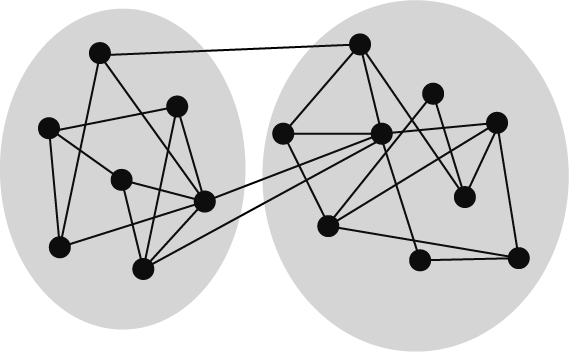
\includegraphics[width=0.5\linewidth]{foundations/ch1/Images/nonattr_ex.png}
\caption[School network hypothesis]{A school network, where the nodes are students and the edges indicate which pairs of students are friends.}
\label{fig:ch1:nonattr}
\end{figure}


Some examples of non-attributed network learning systems are:
\begin{itemize}
\item network embeddings in Section \ref{sec:ch6},
\item community detection in Section \ref{sec:ch7:comm_detect},
\item latent position comparisons in Section \ref{sec:ch8:twosample}, and
\item anomaly detection in Section \ref{sec:ch9:anomaly}.
\end{itemize}


\subsubsection{Attributed network learning systems}

Similarly, the concept of an attributed network learning system is analogous to the concept of supervised or semi-supervised machine learning. \textit{Supervised learning} can be loosely defined as a learning problem in which the data you feed to the algorithm includes {labels}, and \textit{semi-supervised learning} can be loosely defined as a learning problem in which the data you feed to the algorithm includes \textit{some} of the labels. A network is an \textit{attributed network learning system} if at the time of analysis, the network(s) you feed your algorithm include attributes in {addition} to nodes and edges. We have four main types of attributed network learning systems. They are:
\begin{itemize}
\item Networks with node attributes,
\item Networks with edge attributes,
\item Networks with network attributes, and
\item Networks with multiple-network attributes.
\end{itemize}


\paragraph{Networks with node attributes}

A network with \textit{node attributes} is a collection of nodes and edges where, for each node, you have an additional piece of information to describe that node. Let’s consider the school example we talked about above in the section on non-attributed network learning systems. For each student, you also have an additional piece of information: you know which school each student attends, and you want to investigate whether the probability of two students being friends is higher in school one or in school two. A problem for networks with node attributes is shown in Figure \ref{fig:ch1:netnode_edge_attr}(A). 

\begin{figure}[h]
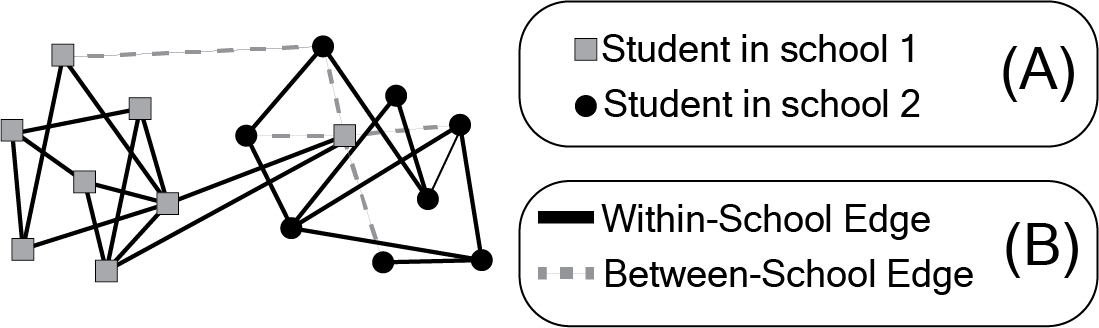
\includegraphics[width=\linewidth]{foundations/ch1/Images/nodeedge_attr.png}
\caption[School with node and edge attributes]{\textbf{(A)} the school network for Facebook, approached using node attributes. \textbf{(B)} the school network for Facebook, approached using edge attributes. Instead of focusing on the school assignments of the nodes, we focus on two groups of edges (the within-school edges, and the between-school edges).}
\label{fig:ch1:netnode_edge_attr}
\end{figure}


Some examples of problems which deal with node attributes are:
\begin{itemize}
\item 

joint representation learning in Section \ref{sec:ch6:joint},

\item 

model selection in Section \ref{sec:ch7:modelselect},

\item 

testing for differences in block matrices in Section \ref{sec:ch8:twosamplesbm}, and

\item 

testing for differences between groups of edges in Section \ref{sec:ch7:testing}.

\end{itemize}

\paragraph{Networks with edge attributes}

A network with edge attributes is a network consisting of nodes and edges where, for each edge, you have an additional piece of information to characterize that edge. For instance, if we return to the Facebook school network from Example \ref{box:ch1:social} that we posed above, we could entirely ignore the school assignments, and simply focus on whether the students have more friends within schools (solid edges) or between schools (dashed edges). This example is shown in Figure \ref{fig:ch1:netnode_edge_attr}(B).


A problem with edge attributes is testing for differences between groups of edges in Section \ref{sec:ch7:testing}.


\paragraph{Networks with network attributes}

A network with network attributes is a collection of networks (each of which has nodes and edges) where, for each network, you have an additional piece of information to characterize that network. Returning to Example \ref{box:ch1:brainnet}, each brain network was from either a musician or a non-musician. This piece of information characterizes each of the networks as either from a musician or a non-musician individual, and applies to the {entire} collection of nodes and edges for a given network. A network with network attributes is shown in Figure \ref{fig:ch1:netnetattr}.

\begin{figure}[h]
\centering
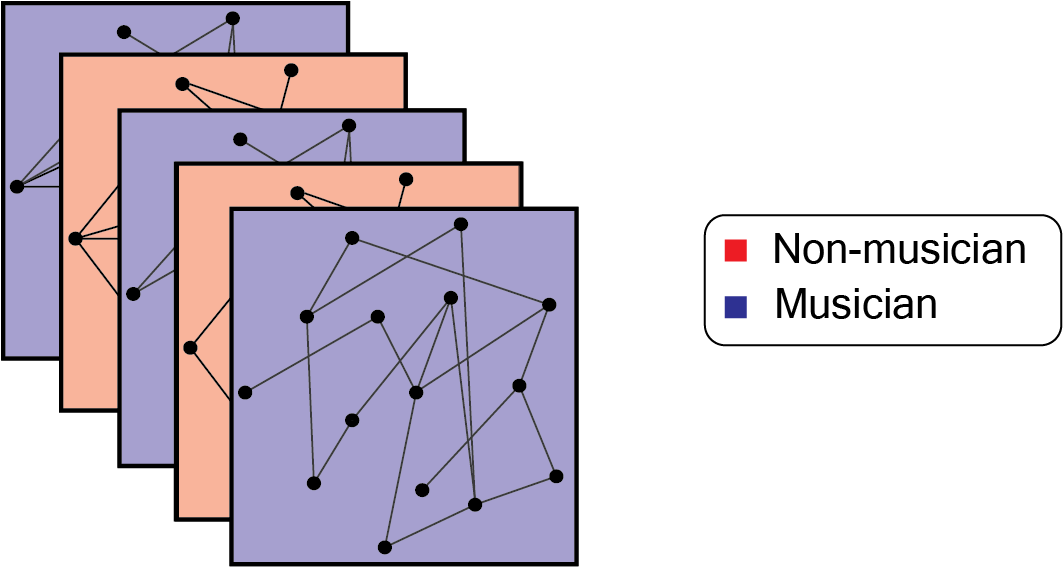
\includegraphics[width=0.8\linewidth]{foundations/ch1/Images/netattr_ex.png}
\caption[Brain networks]{A collection of brain networks, where the nodes are areas of the brain and the edges indicate which brain areas can communicate. For each network, you know whether it comes from a musician or a non-musician.}
\label{fig:ch1:netnetattr}
\end{figure}


An example of a problem which leverages network attributes are signal subgraphs in Section \ref{sec:ch9:ssn_incoherent}.


\paragraph{Networks with multiple-network attributes}

A network with \textit{multiple-network attributes} is a collection of networks (each of which has nodes and edges) where you have additional information that describes how the nodes (or the edges) of the networks relate to one another. Returning to Example \ref{box:ch1:social}, let's add another dimension. The accounts are, for all intents and purposes, anonymous, in that people choose not to share identifying information about themselves on the accounts. However, for three of the people, you know that their two accounts are {matched} together. You want to see if you can use this cross-network attribute (the {matched accounts}) to discover suitable matchings for the remaining accounts in the network. A problem with multiple-network attributes is shown in Figure \ref{fig:ch1:netmultiattr}.

\begin{figure}[h]
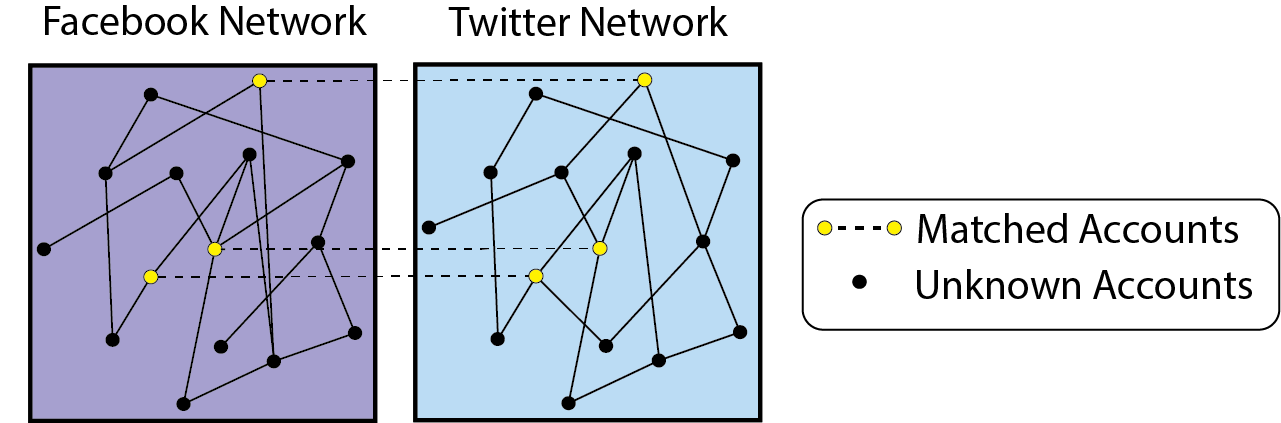
\includegraphics[width=\linewidth]{foundations/ch1/Images/crossnetattr_ex.png}
\caption[Multiple network attributes]{Two social networks from different social media sites. The nodes are people’s accounts on the social media sites (they are the same for both sites) and the edges indicate which pairs of accounts follow one another for that particular site. For three of the people in the network, you know their accounts.}
\label{fig:ch1:netmultiattr}
\end{figure}


An example of problems which leverage cross-network attributes include:
\begin{itemize}
\item Seeded graph matching in Section \ref{sec:ch8:gm}, and
\item Vertex nomination for two networks in Section \ref{sec:ch8:vnviasgm}.
\end{itemize}

\subsection{What part of the network your question is asking about}

In network machine learning, it’s easy to get lost because you're tempted to explore the entire network, whereas your question might be far more limited. For instance, in a transportation network, you might have a collection of nodes representing stations, and a collection of edges representing the number of riders per train during rush hour. You might have a single network for each week of the entire year. We’ll show an example of each type of question from the perspective of the attributes of these networks. 
\begin{enumerate}
    \item Studying a single edge: You might want to know whether a particular edge between two stations could require an additional train because the route is popular during rush hour, and you might only want to study this particular edge over many networks to get some idea of how many passengers take each train.
    \item Studying a single node: You might want to explore the number of passengers who pass through a particular station when deciding whether to approve or reject the expansion of a particular station to include more platforms.
    \item Studying groups of nodes or edges: You might consider cancelling an entire line and need to consider the ramifications of this decision on other stations (groups of nodes) and numbers of passengers per line (groups of edges).
    \item Studying the entire network: You might need to determine whether more funds need to be allocated to public transportation as a whole, and therefore to study how much transportation via the network saves the city over the course of the year.
\end{enumerate}


\subsection{Model-based vs non-model-based network learning systems}

Statistics tends to form somewhat of a ``core'' to network learning systems. This is because in any network learning problem, there is always room for randomness, whether it comes in the form of the particulars of the network you sampled, the set of networks you acquired, the nature of the data you collected, or many other factors. 

We will provide a more rigorous definition later, but for now, you can understand a \textit{statistical model} to be a conceptual framework of a problem that allows you to explicitly account for variation, randomness, or error in your sample (the data you actually obtain) compared to the entirety of the actual object or set of objects that you are studying (the \textit{population}). This balance between model-based and non-model-based network learning is a core aim of this book, so we do not expect you to be able to conceptualize the difference just yet. For this reason, we will try to explain the difference without talking about networks for now.


\subsubsection{Model-based learning systems}

A \textit{model-based learning system} is a system in which a statistical model is required in order to derive your intended meaning from an analysis.

Imagine that you have two coins, and you flip each of them twenty times. You want to understand whether the probability that the two coins land on heads is the same or different. What this means in statistics is that you want to perform a {hypothesis test}: you want to use the data that you obtained (the outcomes of the twenty coin flips for each of the two coins) to determine whether the coins have the same probability of landing on heads (the first hypothesis) or a different probability of landing on heads (the second hypothesis). The \textit{hypothesis test} is the procedure to determine which of the two hypotheses is better supported by the data. This question cannot really be made sense without using a statistical model, because the term {probability} has a statistical interpretation. If you wanted to answer this question, you would need to describe several factors about your experiment a little further:
\begin{itemize}
\item Can each of the coins {only} land on heads or tails, or is there perhaps some other possible outcome? For instance, is one of the coins one centimeter thick and the other a picometer thick, and therefore, the centimeter thick coin has a nonzero probability of landing on its side?
\item For each coin, is the probability that the coin lands on heads {exactly the same} across each of your twenty coin flips for that particular coin? For example, if you flip the coin differently for the first ten flips than you do on the last ten flips, could this artificially make the coin land on heads more or less frequently?
\item Do the outcomes of the coin flips depend on other coin flips? For instance, if you see two straight tails in one of the coins and say a prayer that you get a heads on the next flip, does this affect the probability that the next flip is a heads?
\item Did you collect enough data to determine whether the coins are different? For instance, many statistical tests (including this one) can be interpreted in a variety of ways. When the sample size is tiny, we need to be careful about the assumptions that we make, because statistical testing approaches that we might use (the chi-squared test, for instance) might only be meaningful when we have a lot of data.
\end{itemize}

In order to make a conclusion based on your hypothesis test, you need to be very specific about the assumptions you make about these details of the your data sample, since if any of your assumptions are false, the answer to your question might have a different interpretation. Therefore, you need to understand the assumptions that you made, so that you can make a {decision} based on the outcome of the hypothesis test that you performed.


\subsubsection{Non-model-based learning systems}

For many questions you might want to ask, you could apply techniques from this book in either a model-based or non-model-based manner and be fine either way. What we mean by this is that a lot of questions might be made {intuitive} using a model, but there is no reason you {need} a model in order to answer these questions. A \textit{non-model-based learning system} is a system in which a statistical model is {not} required in order to derive meaning from an analysis.

To make this type of machine learning system a little more concrete, we’ll break down a traditional non-model-based machine learning system. \textit{Principal components analysis} is a procedure which takes data which is {wide} (it has a lot of features or dimensions, which is extremely problematic for many machine learning approaches) and makes it narrower (it has a manageable number of features or dimensions) so that you can use other strategies downstream which might be{more reasonable}, by which we mean that each observation starts with many features, but after applying \texttt{PCA}, each observation has far fewer features. A visual illustration of \texttt{PCA} is shown in Figure \ref{fig:ch1:pcaex}. In this example, we reduce the data from two dimensions (indicated by the $x$ and $y$ axes) to one dimension along the red axis (the first PC).

There is no reason that this procedure cannot be {executed} knowing nothing else about the data: it is simply an algorithm which produces a desired result (making the data manageable for other machine learning techniques). However, if you were to do this and use the intuition of a statistical model (specifically, that the observations are {normally distributed}), you can understand the principal components to be representations of the data that preserve the most {variation}. You can understand variation in this context to be the direction that the data spreads along the most: in Figure \ref{fig:ch1:pcaex}(A), notice that the black points tend to spread out a lot along the red PC, but not as much along the green PC. The degree of variation preserved by the principal components, if you recall, are indicated by principal component scores. This is often desirable intuition for machine learning because if you wanted to apply say \texttt{K-Means} to cluster your observations, you will need the observations from each class to “look” different -- and “looking different” requires variability.

\begin{figure}[h]
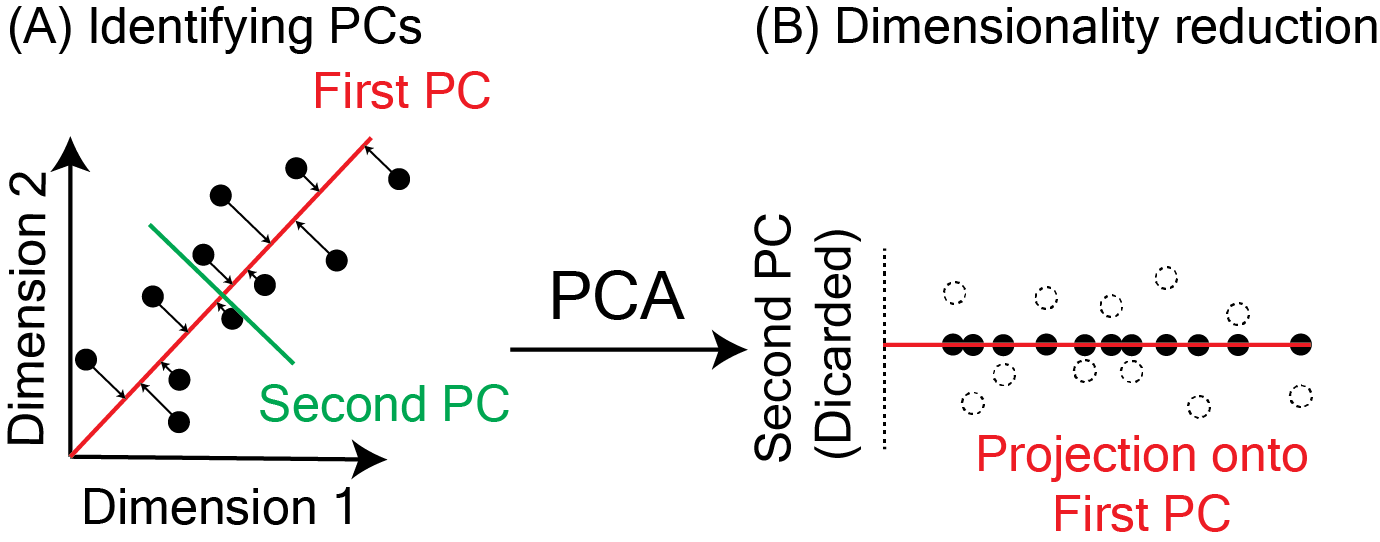
\includegraphics[width=\linewidth]{foundations/ch1/Images/pca_ex.png}
\caption[Principal components analysis]{\textbf{(A)} the observed data shown in the left scatter plot, where the points are two-dimensional. The first ``principal component'' (PC) is the axis in which the data varies the most, and the second PC is the axis (orthogonal to those of the preceding principal components) along which the data varies the second most. Projecting the data to the first PC is shown with the arrows. \textbf{(B)} the data is ``projected'' onto the first PC via PCA, by effectively ``reorienting'' the dataset along the first and second principal components (dashed circles and lines), and then removing the second PC entirely (solid circles) to reduce the dimensionality from two dimensions to one dimension. Think about this in a model-based manner, we ``discarded'' a direction in which the data varies less.}
\label{fig:ch1:pcaex}
\end{figure}

\newpage
\section{Challenges of network machine learning}
\label{sec:ch1:challenges}

Like other branches of science, network machine learning is not without its challenges. There are infinitely many ways in which your network, or networks, that you actually get to analyze might have imperfections which can most efficiently be described as random. Rather than collecting data from every single person on the social network, or obtaining brain networks from every single person who could {potentially} be a musician, or collecting pristine data that always represents the underlying network perfectly, you instead look at a reasonably sized subset of data which you can feasibly obtain. Maybe this means collecting your social network with only $1000$ nodes instead of one hundred million, or maybe this means looking at $200$ brain networks instead of a network from every person in the United States.

In this book on network machine learning, we are going to focus some level of attention on the sub-branch of machine learning known as statistical learning. \textit{Statistical learning} is a framework for machine learning in which we {infer} things about our network by using statistics to refine and conceptualize our problem and quantify how reasonable our conclusions are. What exactly do we mean by this?

\subsubsection{We might imperfectly observe the network}

In many branches of science, collecting network data can be an imperfect and noisy process. It was only recently that we acquired a detailed map of the connectome of a complex organism, the fruit fly larva \cite{Winding2023Mar}. Even though fruit fly larvae are small, this is a substantial undertaking: their brain comprises several thousand neurons, and hundreds of thousands of edges, all fit into a volume smaller than cubic millimeter. In order to study the brain at the neuron-scale, the brain was sliced into thousands of tiny pieces smaller than a human hair, and each piece individually examined with a microscope. From there, extremely complicated algorithms and manual tracing were performed to stitch, slice-by-slice, which neurons connected with which neurons. To make this process even more difficult, everything was done on a single organism; with each step there was extremely minimal room for error. This neuron-by-neuron map was used to construct a network (called the \textit{connectome} of the organism) where the nodes were neurons and the edges were the neuron-to-neuron connections.

\begin{figure}[h]
    \centering
    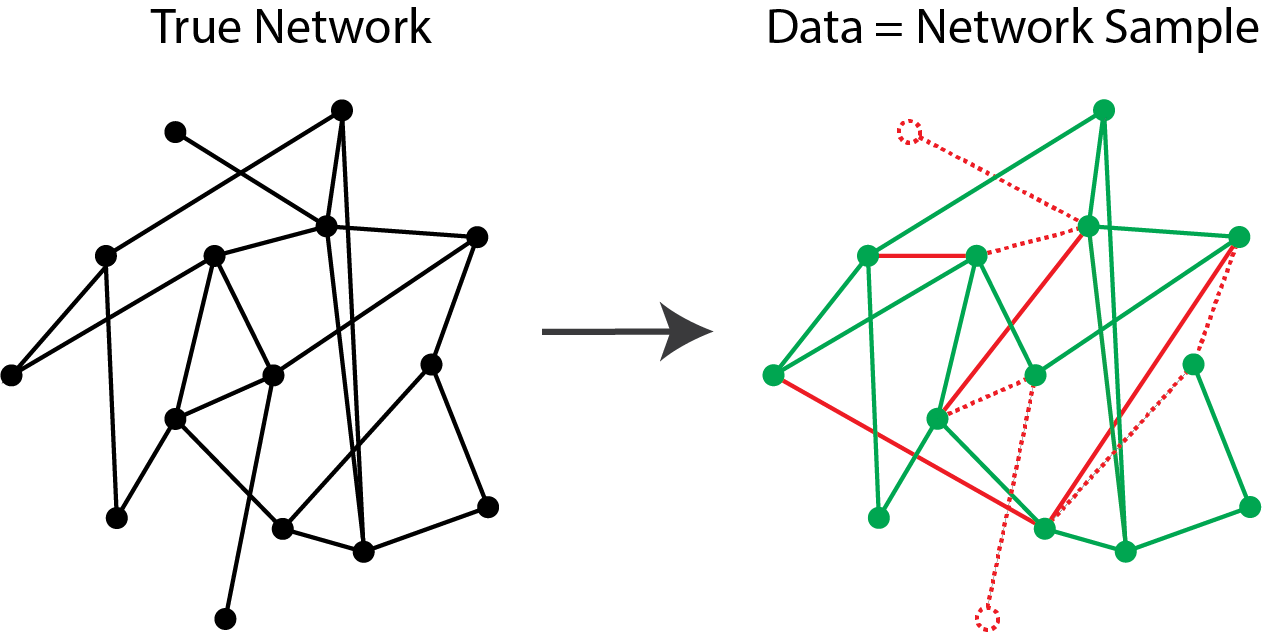
\includegraphics[width=0.7\linewidth]{foundations/ch1/Images/errorful_obs.png}
    \caption[Errorfully observe networks]{The true underlying network contains a lot of information that in the
course of observing or sampling the network, we don't actually measure properly. }
    \label{fig:ch1:errorful_net}
\end{figure}

With so many areas for potential error, it is almost impossible that the network is absolutely perfect. We might have missed some neurons, we might have missed some connections, and there might have been small mistakes anywhere in this complicated process. Figure \ref{fig:ch1:errorful_net} explores what it means for a network to be imperfectly observed. On the left, we see the true network we're trying to obtain. On the right, we see the actual network we obtained: we might be missing some of the nodes (red dashed nodes), we might be missing some of the edges (red dashed edges), or we might see edges which shouldn't really be present (red solid edges). While a portion of the network might faithfully represent the underlying system (green nodes and edges), we don't actually get to see what part of our sample is faithful or unfaithful with respect to the underlying network. The key is that when we attempt to build network machine learning systems, we need to be able to derive insights that are robust to these imperfect observations. This is because in some cases, it might be impossible to ever obtain the data that we need otherwise.

\subsubsection{We might not see the whole network}

When we study a network, it is rare that we observe the entire system perfectly in its entirety. For instance, a social network, in which the nodes of our network are people within the network, and edges are whether groups of people are friends with one another. If we wanted to study the network in its rawest form, we might need to collect data from millions, or billions, of accounts to construct a network that might take an infeasible amount of space just to store. Actually analyzing the network represents another huge hurdle; we would need to be able to devise techniques which could efficiently churn through terabytes worth of data. On the other hand, perhaps we could focus our attention on a subset of the network involving a few thousand or hundred thousand people. On this reduced subset of people, we might be much more free to ask rich questions, as we might not be nearly as limited in terms of the techniques that we can use on the data in a feasible time frame.

On a related note, the example that we gave for the fruit fly larva (drosophila) connectome was certainly not the first time connectomes have ever been investigated; people have been studying brain networks for decades. Before that paper came out, in fact, the drosophila larva has been a major focus of many connectome analyses. Due to the massive economic, computational, and anaytical challenges, however, earlier investigations focused on subsets of the brain, rather than on the whole thing. Despite only collecting bits and pieces of the network, major insights were learned which directly informed the effort to collect the entire network.

In both of these cases, you can learn a lot of valuable information by reducing the size of your network, learning from it, and then applying what you learned to the entire network. In Figure \ref{fig:ch1:nodes_ss}, we see an example where we only get to see a subset of the nodes in the network.

\begin{figure}[h]
    \centering
    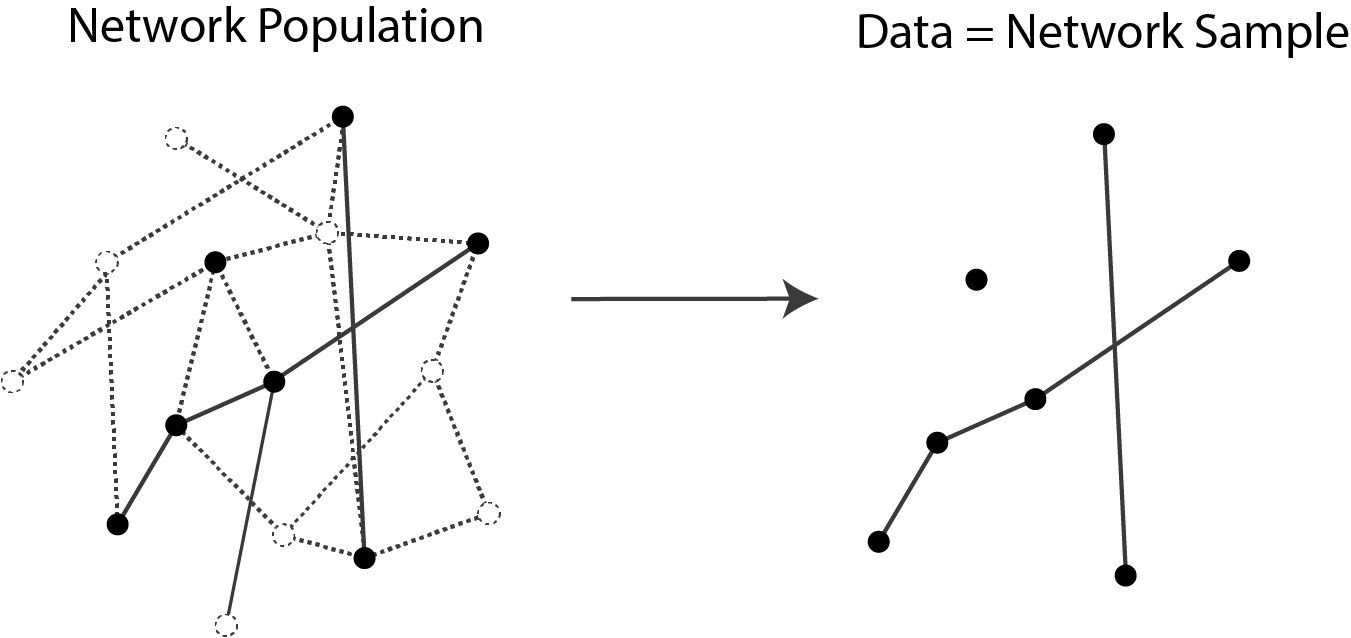
\includegraphics[width=0.8\linewidth]{foundations/ch1/Images/nodes.png}
    \caption[Only see subset of nodes]{The true underlying network has both solid and dashed edges and nodes, indicated in the left panel. However, when we sample the network on the right, our sample only includes the subset of nodes and edges that are solid.}
    \label{fig:ch1:nodes_ss}
\end{figure}


\subsubsection{We might only see a subset of the networks}

On a related note, let's put ourselves back in the mindset for the musician and non-musician brain networks from Example \ref{box:ch1:brainnet}. A team of psychologists might hypothesize that the brains of musicians tend to be much better connected in areas responsible for fine motor coordination and hearing, which are crucial skills for many instruments. To test this hypothesis, the psychologists could take one of two approaches. They could collect brain networks from every individual, or they could collect a subset of brain networks from groups of musicians and non-musicians in their area. In Figure \ref{fig:ch1:many_nets_ss}, we see an example where we only get to sample a subset of the networks in the underlying population. Despite the fact that the psychologists only studied a subset of musicians and non-musicians, with some statistical assumptions they can derive conclusions that will apply more broadly than just the group of people they analyzed.

\begin{figure}[h]
    \centering
    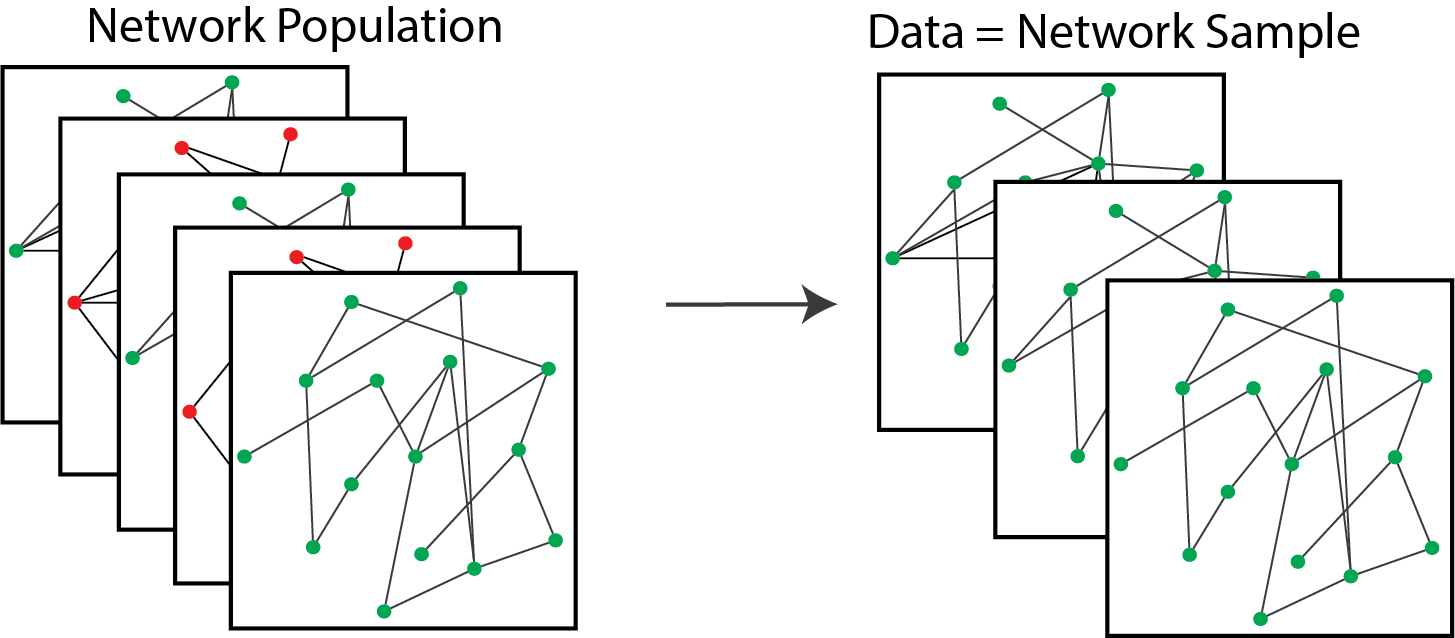
\includegraphics[width=0.7\linewidth]{foundations/ch1/Images/many_networks.png}
    \caption[Only see subset of networks]{The true underlying population contains many more networks than we are
able to actually sample. In the left panel, we have green and red
networks, but in the sample, we only get to see the green networks.}
    \label{fig:ch1:many_nets_ss}
\end{figure}

\subsubsection{Statistics allows us to bridge what we learn from what we see with what we didn't get to see}

In these cases, you have collected a \textit{sample}, which can be loosely defined as a subset of objects which is collected from the population in some way. The sample itself is where statistics comes into play. When you reach a conclusion, you do not want to reach a conclusion that only applies to the specific group of people, or the specific network, that you analyzed in your sample. Statistics allows you to be as specific as you can about how, exactly, conclusions that you reach on the sample apply to the general population. We summarize this idea in Figure \ref{fig:ch1:stat-learning}. Note that the network population may have a different interpretation depending on you specific network question, and might be populations of many networks, or populations of networks with some level of randomness or uncertainty as to how the network was obtained. Throughout this book, the sample itself, and how it relates to the underlying population, will always be in focus and should be at the forefront of your mind. 

\begin{figure}[h]
    \centering
    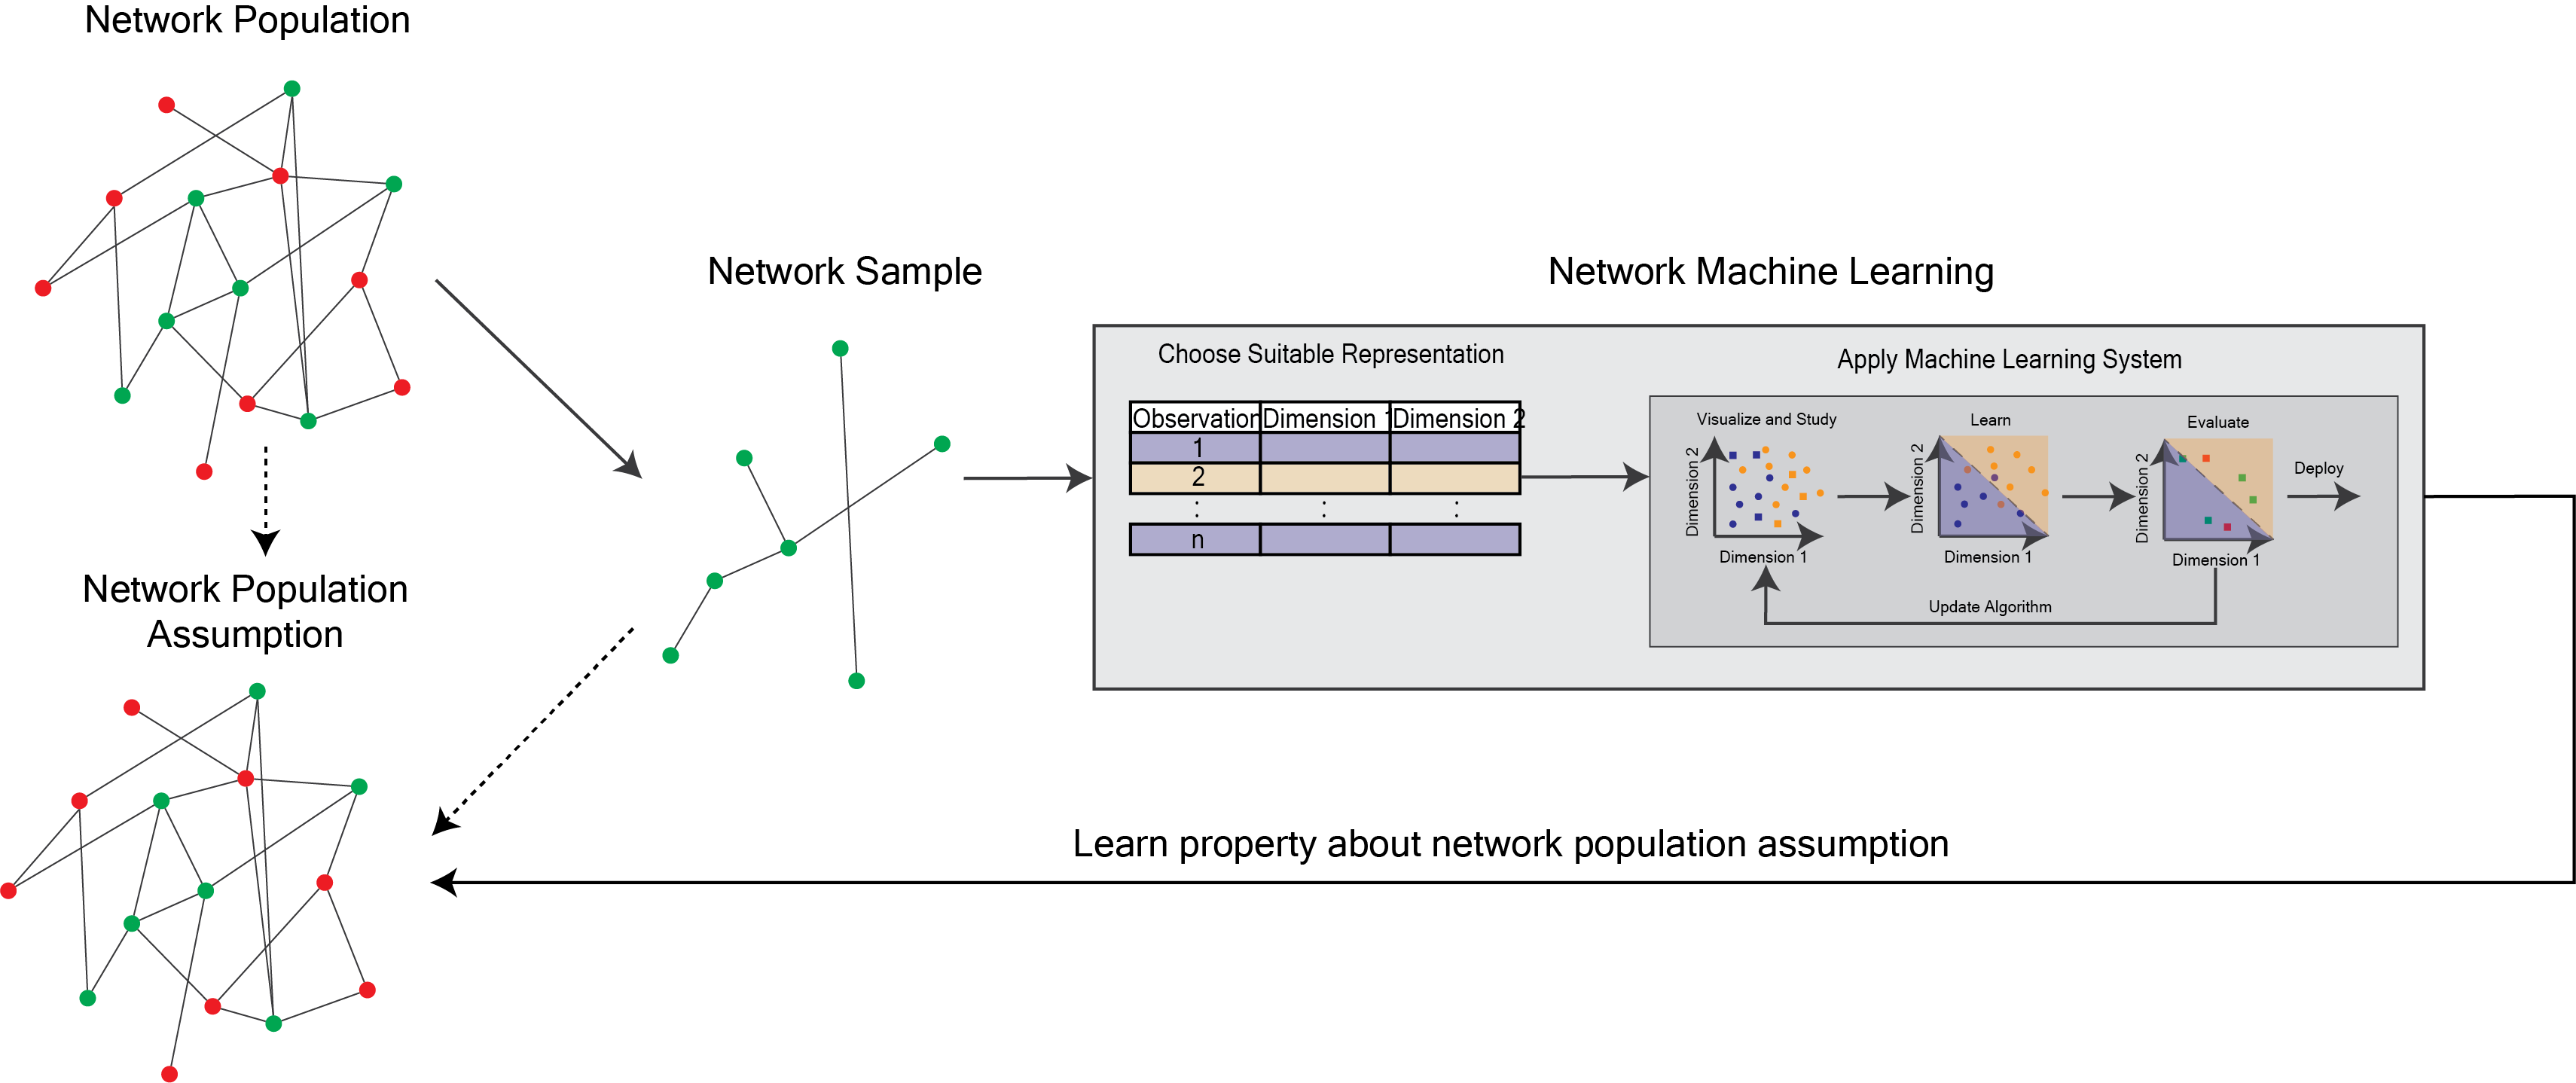
\includegraphics[width=\linewidth]{foundations/ch1/Images/apply.png}
    \caption[Statistical network machine learning]{We have a network population, which in this case, means a large network that we cannot properly observe. We obtain a sample of this network, and then use analyses on this sample and knowledge of how this sample was taken from the population to derive assumptions about our system. Ideally, this will faithfully represent the actual network population itself. Using network machine learning, we learn properties about the network population assumptions.}
    \label{fig:ch1:stat-learning}
\end{figure}


You {can} learn lots of valuable things about a sample without using statistics {at all}, and we will be sure to note when that is the case. However, if you want your conclusions to apply more broadly to the general population rather than the specific sample you collected, a reasonable way to do that quantitatively is using statistical learning.

\subsection{There are a variety of other challenges too!}

In Section \ref{sec:ch1:types}, you learned about some of the different types of network machine learning problems that we can start to address. Network machine learning is in its infancy, and these types of problems are constantly evolving. Deciding which group of categories your problem falls into, reshaping your question of interest to fit into problems that can be answered with existing techniques, the types of strategies that are at your disposal to answer your questions, or whether you need to develop new techniques all together to answer your question take lots of energy (and resources!). In the next few chapters, you'll see what example data analyses look like in network machine learning, which will hopefully give you a better idea of how these analyses are performed.

\newpage


\bibliographystyle{vancouver}
\bibliography{references}
\chapter{End-to-end Biology Network Machine Learning Project}
\label{sec:ch2}

In this chapter, we try to motivate network machine learning with some behind the scenes work, to give you a feel for what the process is really like from start to finish. While some of the material in this section might seem a little bit opaque at first, we try to keep the details lighter and the big picture in focus. You can jump around with network machine learning in a real setting, before we start jumping right into the nitty, gritty details. This will give you a chance to ensure that you have all of the dependencies set up appropriately from the beginning. Things run a lot smoother, in our experience, when you start with a working programming environment. We have the following sections:
\begin{enumerate}
    \item Section \ref{sec:ch2:bigpicture} discusses how to approach a network machine learning problem.
    \item Section \ref{sec:ch2:getdata} establishes how to set up your local environment to use this textbook, and how to grab some example data. 
    \item Section \ref{sec:ch2:prepare} details how to prepare your data for downstream analysis.
    \item Section \ref{sec:ch2:select} covers the algorithm selection process for network data.
    \item Section \ref{sec:ch2:finetune} demonstrates the tuning process for network machine learning algorithms.
    \item Section \ref{sec:ch2:discover} illustrates how we can use network machine learning to uncover new insights about network data.
\end{enumerate}

\newpage 

\section{Looking at the big picture}
\label{sec:ch2:bigpicture}


Welcome to the Neurobiology Institute! A colleague has come to you with an interesting problem. Brains consist of neurons. Different patterns in which these neurons connect produce the unique functions your brain is able to do: it is able to manage functions like breathing, as well as more active functions like moving, hearing, seeing, and higher level thought.

When they are electrically stimulated, neurons transmit that electrical signal to other neurons. This process consumes a lot of energy for your body; while the brain is only about 2\% of your weight, it consumes about 20\% of the energy your body uses per day. To keep the neurons replenished with energy (and to remove waste that the cells produce when they work), the brain has a complicated network of blood vessels. When a brain area is in use, the body dedicates blood supply to the area that will need it most.

Neurobiologists came up with a rather clever way to decipher brain activity in humans by looking at this blood flow. Using MRI, they can trace the particular areas that the blood was flowing towards. Scientists were able to demonstrate that this signal really did tend to correlate with brain activity. 

\begin{figure}[h]
    \centering
    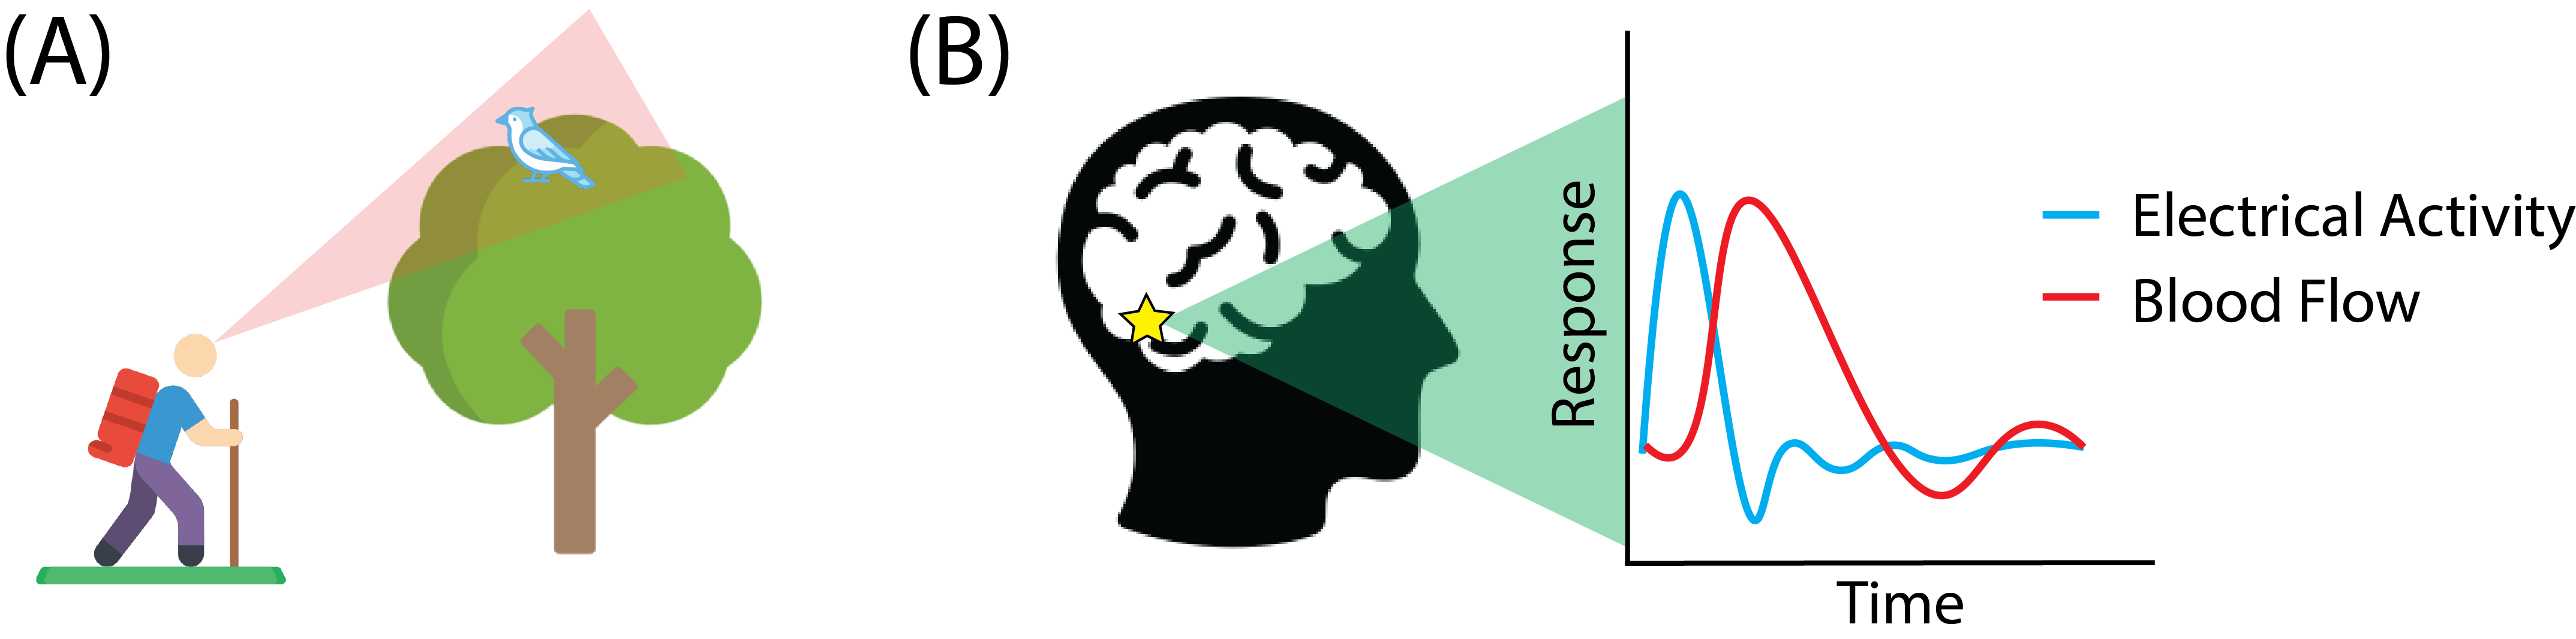
\includegraphics[width=\linewidth]{foundations/ch2/Images/fmri_bold.png}
    \caption[BOLD f-MRI]{(A) A hiker out on the trails sees a bird pirched in a tree in his field of view (faint red triangle). (B) The occipital lobe, which is responsible for sight, sits in the back of the brain (star). The presence of the bird in the field of view causes neurons to be electrically stimulated (blue line). The activity of the neurons causes the brain to send blood to the area as the neurons are stimulated (red line). While individual neurons are too small to see, the blood flow of many neurons in the brain can be picked up by the fMRI scanner.}
    \label{fig:fmri-bold}
\end{figure}

This imaging technology, known as functional MRI, has proven to be interesting to neuroscientists \cite{Poldrack2011Aug}. By measuring pairs of brain areas, researchers can see whether the two areas tend to be active together. The idea is that, perhaps, different combinations of brain areas tend to work together as a unit, allowing the complicated thought patterns that humans are capable of. By viewing the different areas of the brain as nodes of a network, and the correlations as the edges, scientists have constructed networks from this line of thinking. This area of study, called connectomics, presents an extremely network-centric area of research \cite{Munsell2018Sep}.

Your colleague has come to you with a bunch of networks from fMRI sessions, and wants to know whether there are any higher level groups of brain areas that tend to have similar activity. Can you, as a network scientist, take this network of nodes and edges, and figure out a way to break the nodes into groups of nodes which are functionally similar?

\subsection{Framing the problem}

The first question to ask your colleague is; what exactly is the objective here? In network machine learning, the choice of the model used is \emph{everything}. The model determines what sorts of questions we are capable of asking, and what sorts of \emph{answers} we are capable of learning. Asking about the objectives will directly shape which models and approaches you use.

Your colleague wants to know whether there are any sub-groups of areas that tend to behave similarly. By ``behave similarly'', what your colleague means is, are there sub-groups of brain areas that tend to work together in conjunction with other sub-groups of brain areas?

The next question is what we've tried so far. This will prevent you from repeating work, help you understand where to start approaching the problem, and give you a reference for the performance of your techniques. 

Next, you need to determine what type of network machine learning problem you have. What type of data do you have? Do you have any covariates associated with that data? What type of question do you want to answer? Do you want to test a hypothesis, or make predictions? What characteristics will your model need to reflect to be able to answer the question appropriately? Before you progress further, you should answer these questions for yourself. 

Remembering back to the types of network machine learning problems in Section \ref{sec:ch1:types}, you conclude that this is a multiple network learning problem. Your networks are non-attributed, since you only know the nodes and edges of the network. The question asks about groups of nodes and edges, and you hope to use network modelling approaches to study your problem. You are going to need to come up with a definition of what it means for pairs of areas to be similar, and you are going to want to be able to group areas in a way that is meaningful for your colleague.

\subsection{Check the assumptions}

Throughout the course of this book, we will try to keep in direct focus the assumptions being made by the techniques you might pick. You want to choose the simplest set of assumptions that can reasonably reflect the data. This means that you want to use the simplest statistical model that can answer the question you want to address. In this case, we don't care about individual brain area-to-brain area connections at all: we only care about how groups of brain areas behave in relation to other groups of brain areas. This means that we want to choose models which will allow us to learn about pairs of brain area groups, which is a very different problem from learning about individual brain areas themselves.

After talking over your understanding of the problem with your colleague, you are confident that he wants a way to be able to group brain areas together based on how similar they are, and you have the freedom to define that however you choose. You have the green light to begin coding!

\newpage
\section{Getting the data}
\label{sec:ch2:getdata}

For this section, you will start to get your hands dirty with some real network datasets. Don't be afraid to walk through these examples with your laptop in a jupyter notebook. To ease your ability to interact directly with the code of this book, we've developed a standalone \texttt{docker} container that you can use. 

\subsection{Interacting with the book via \texttt{docker}}

Getting software to run across multiple operating systems, particularly software with lots of dependencies, can range from difficult to impossible. While most of the packages required to run the contents of this book can be installed relatively easily via a combination of git, pip, and virtual environments, the easiest and fastest way to get you coding and interacting with real \texttt{python} code is \texttt{docker}. 

\texttt{docker} is a containerization utility that, in effect, allows you to run standalone software in a separate area of your computer (called a {docker container}), that allows software to operate without conflicting with your local operating system. This means that you can, with a very small number of button clicks, create deployable software that thousands of people can use at the drop of a hat. It might not be better than sliced bread, but it might be the next best thing! 

We aren't going to sit here and pretend to be the experts on docker, but fortunately the people over at docker won't leave you on your own for that one! To install docker, check out their installation guide at \cite{dockerinstall}. 

\subsubsection{Obtaining the docker container for the textbook}

Once you have docker installed on your computer, you can obtain the docker container for the book relatively easily. If you have a ubuntu/mac operating system and the docker daemon running on your computer, you can open up a terminal session and type the following command:

\begin{lstlisting}[style=bash]
$ docker pull neurodata/graph-stats-book
\end{lstlisting}

which will fetch the docker container for the book from \cite{thisbookdocker}.

This docker container contains all of the dependencies needed to run the code within this book, and will allow you to use the book in conjunction with \texttt{jupyter}. \texttt{jupyter} is a lightweight, web-based interactive computing platform that you can access through your web browser at \texttt{localhost:<port>}, where \texttt{<port>} is the port you provide to the container for execution. You can start the docker container like this:

% \begin{lstlisting}[style=bash]
% $ docker run -it --rm -p <port>:8888 neurodata/graph-stats-book \
%     jupyter-lab --ip=0.0.0.0 --port=8888 /home/book/ \
%     --NotebookApp.token="graphbook"
% \end{lstlisting}

\begin{lstlisting}[style=bash]
docker run -it -v <path/to/local/working/directory>:/home/book -p 8888:8888 neurodata/graph-stats-book \
    jupyter-lab --ip=0.0.0.0 --port=8888 /home/book/ \
    --NotebookApp.token="graphbook"
\end{lstlisting}

Which will launch a \texttt{jupyter-lab} session, and {should} automatically log you into the session in your browser. If it does not, open up a browser of your choice, and go to \texttt{localhost:<port>}, where you will be prompted to enter the log-in password for your session- that login-in password is \texttt{graphbook}, generated from \texttt{--NotebookApp.token} in the command above. If you don't know what port to choose, it's probably easiest to try \texttt{8888}, and if that doesn't work, \texttt{8889}, and keep working up until you find an open port. The port is so that your browser can communicate with the jupyter session inside the docker container (which runs jupyter internally on port \texttt{8888}), and so you are basically telling your computer that your port \texttt{<port>} should "tie in" to port \texttt{8888} in the docker container.

If you don't want to use the docker container, that's fine too: you can follow the instructions at the end in Section \ref{sec:ch2:get:install} for more details. 

\subsection{Downloading the data}

When you work with network data, it is rarely the case that the {raw data} that you will use is already a network. The \textit{raw data} is the least processed version of the data for your project, and is the information upon which the rest of your data is {derived}. A \textit{derivative} is a piece of data or information that is {derived} from the raw data. Consider, for instance, that you are investigating emailing trends for a company, and trying to see whether employees tend to email their team members more or less frequently than people outside of their team. In this case, your raw data might be a list of emails, coupled with the sender, and the recipient, of each email. You might be responsible for {preprocessing} this data to acquire a network derivative for your later analyses.

In this section, you won't worry just yet about preprocessing a raw dataset, and will instead start with some pre-prepared data. You will be working with brain networks from a human functional MRI connectome. You could navigate over to the \texttt{neurodata} website and download the file directly, but it tends to be useful to get used to how to do this programmatically. This is because if the data changes, you might want your analysis to automatically update and pertain to the latest and best version of the data at the time you execute your function. Further, if you intend your code to be reproducible, having a function which downloads and prepares the data in a way which the computer can use will simplify the process of disseminating your work. 

To begin, we'll start with a code snippet which fetches the required data for our analysis:

\begin{lstlisting}[style=python]
import os
import urllib
import boto3
from botocore import UNSIGNED
from botocore.client import Config
from graspologic.utils import import_edgelist
import numpy as np
import glob
from tqdm import tqdm

# the AWS bucket the data is stored in
BUCKET_ROOT = "open-neurodata"
parcellation = "Schaefer400"
FMRI_PREFIX = "m2g/Functional/BNU1-11-12-20-m2g-func/Connectomes/" + parcellation + "_space-MNI152NLin6_res-2x2x2.nii.gz/"
FMRI_PATH = os.path.join("datasets", "fmri")  # the output folder
DS_KEY = "abs_edgelist"  # correlation matrices for the networks to exclude

def fetch_fmri_data(bucket=BUCKET_ROOT, fmri_prefix=FMRI_PREFIX,
                    output=FMRI_PATH, name=DS_KEY):
    """
    A function to fetch fMRI connectomes from AWS S3.
    """
    # check that output directory exists
    if not os.path.isdir(FMRI_PATH):
        os.makedirs(FMRI_PATH)
    # start boto3 session anonymously
    s3 = boto3.client('s3', config=Config(signature_version=UNSIGNED))
    # obtain the filenames
    bucket_conts = s3.list_objects(Bucket=bucket, 
                    Prefix=fmri_prefix)["Contents"]
    for s3_key in tqdm(bucket_conts):
        # get the filename
        s3_object = s3_key['Key']
        # verify that we are grabbing the right file
        if name not in s3_object:
            op_fname = os.path.join(FMRI_PATH, str(s3_object.split('/')[-1]))
            if not os.path.exists(op_fname):
                s3.download_file(bucket, s3_object, op_fname)

def read_fmri_data(path=FMRI_PATH):
    """
    A function which loads the connectomes as adjacency matrices.
    """
    # import edgelists with graspologic
    # edgelists will be all of the files that end in a csv
    networks = [import_edgelist(fname) for fname in tqdm(glob.glob(os.path.join(path, "*.csv")))]
    return np.stack(networks, axis=0)
\end{lstlisting}

Now when you call \texttt{fetch\_fmri\_data()}, it creates a new directory called \texttt{datasets/fmri} in your workspace, and downloads the adjacency matrices, the standard way to represent a graph as a mathematical object, into your local directory \texttt{datasets/fmri}.

Next, we'll try to load the dataset using the \texttt{graspologic} utility, \texttt{import\_edgelist()}:

\begin{lstlisting}[style=python]
fetch_fmri_data()
As = read_fmri_data()
\end{lstlisting}

Next, let's learn some things about just one of the adjacency matrices. In network machine learning, when dealing with a new dataset, our recommendation is to {always}, {always}, start with visualization. You typically visualize network data using a heatmap. The resulting plot is shown in Figure \ref{fig:ch2:raw}(A).

\begin{lstlisting}[style=python]
from graphbook_code import heatmap

A = As[0]
ax = heatmap(A, vmin=0, vmax=1, title="Heatmap of Functional Connectome")
\end{lstlisting}

What this has done is it has plotted the adjacency matrix for the functional connectome of a human. The nodes of this network are numbered in sequential order. A heatmap is a network visualization in which the $x$ and $y$ coordinates of a given entry in the matrix indicate the pair of nodes an edge is connected to, and the color for the $(x,y)$ point in the figure indicates the weight of the edge between nodes $x$ and $y$. The edge weight is stronger if the pair of brain areas are active together more, and lower if the pair of brain areas tend to be active together less. This is real data, generated from actual fMRI scans!

One thing that we can notice from this plot is that a lot of these edges have tiny weights. Let's explore this a little bit further. 

A useful summary of the network is to look at a histogram for the edge-weights. A histogram shows the number of edges (on the vertical axis) which have a given edge weight range (indicated by the width of a particular bar on the horizontal axis). You can call this directly on the adjacency matrix (albeit flattened), and it will plot a histogram of the edge weights. We will do this using seaborn's \texttt{histplot()}:

\begin{lstlisting}[style=python]
import seaborn as sns
import matplotlib.pyplot as plt

ax = sns.histplot(A.flatten(), bins=50)
ax.set_xlabel("Edge weight")
ax.set_title("Histogram of functional connectome edge-weights")
\end{lstlisting}
A plot of the adjacency matrix's edge weights is shown in Figure \ref{fig:ch2:raw}(B). A lot of the edge-weights tend to be right around the $0.1$ to $0.5$ range, which tells us that, in general, the nodes of the network are {slightly correlated}. This means that, in general, when some node tends to be active, other nodes also tend to be active. If this were not the case, the histogram would be a bit more centered around $0.0$.

\begin{figure}[h]
    \centering
    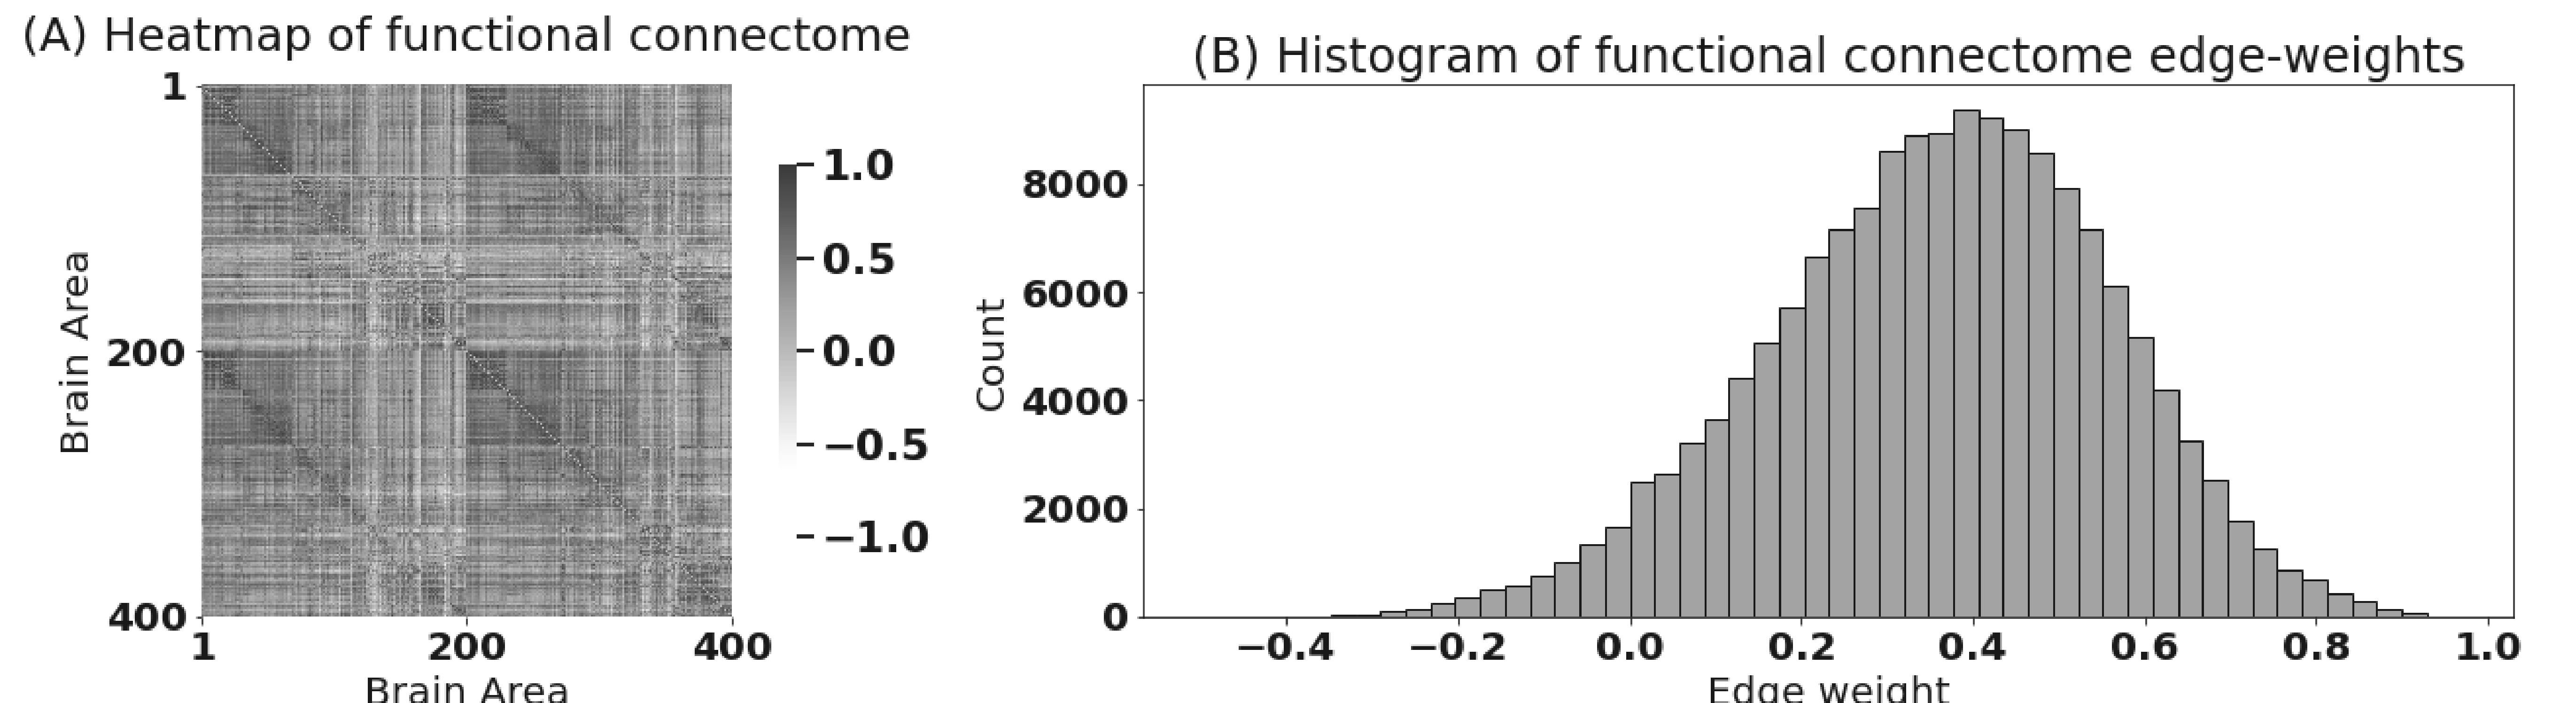
\includegraphics[width=\linewidth]{foundations/ch2/Images/raw.png}
    \caption[Visualizing connectome data]{\textbf{(A)} a raw connectome, \textbf{(B)} the raw connectome edge-weight histogram.}
    \label{fig:ch2:raw}
\end{figure}

\subsection{Create the workspace}
\label{sec:ch2:get:install}
\subsubsection{Installing the latest version of \texttt{python}}

To begin, you will need a suitable instance of \texttt{python} installed. For this book, we'll use \texttt{python 3.8}, but the most advanced version of \texttt{python3} at the time you are reading should do the trick. We will assume that you are using a Linux or UNIX-like operating system, such as OSX. If you have a Windows computer, we would recommend that you use the Docker container or the Linux subsystem module, which you can find more details about in \cite{windowsss} to interact with the codebase. Once you have this set up and up and running, you can follow the instructions below for a Debian distribution of Linux.

Once you have your computer handy, you can run the following command, which should show (ideally) \texttt{python3} has a version $\geq$\texttt{3.8.0}:

\begin{lstlisting}[style=bash]
$ python3 -V
Python 3.8.0
\end{lstlisting}

and verify that the \texttt{python} package manager, \texttt{pip}, is installed:

\begin{lstlisting}[style=bash]
$ python3 -m pip --version
pip 22.0.3 from /<user>/.virtualenvs/graph-book/lib/python3.8/site-packages/pip (python 3.8)
\end{lstlisting}

This command will print the version of \texttt{python3} and \texttt{pip} that your computer currently has installed. If it returns any version below \texttt{3.8.x} or says "command not found", you will need to obtain and install \texttt{python3} (along with the developer libraries and the package manager, \texttt{pip}) before continuing. The developer libraries are critical to ensuring that code upon which packages in \texttt{python} are based (such as the popular \texttt{numpy} numerical package) have the appropriate libraries needed to execute code written in {other} programming languages, which might be faster (for instance, \texttt{C}). 

If you have an apple computer using the OSX operating system, you can download and install an appropriate version of \texttt{python} using the \texttt{python3} guide for OSX at \cite{pythonmac} by first configuring \texttt{homebrew} and then installing python. This will also include \texttt{pip}. 

If you are using a Debian-based Linux distribution (such as Ubuntu), you can install \texttt{python3} along with the developer libraries and \texttt{pip} by typing:

\begin{lstlisting}[style=bash]
$ sudo apt-get update
$ sudo apt-get install -y python3-dev python3-pip
\end{lstlisting}

If you have a CentOS distribution (such as CentOS or Red Hat), you can install python3 along with the developer libraries and \texttt{pip} by typing:

\begin{lstlisting}[style=bash]
$ sudo yum update
$ sudo yum install -y python3-devel python3-pip
\end{lstlisting}

You should make sure that you have the most recent version of \texttt{pip} installed. To upgrade the current \texttt{pip} package, type:

\begin{lstlisting}[style=bash]
$ python3 -m pip install --user -U pip
Collecting pip
[...]
Successfully installed pip-22.0.3
\end{lstlisting}

You now have \texttt{python3}, the \texttt{python} package manager \texttt{pip}, and the \texttt{python3} developer libraries installed on your computer. 

\subsubsection{Installing fortran}

Some of the packages that you will use in the book require the system to have an appropriate version of a programming language called FORTRAN installed. FORTRAN is a numerical programming language which is very fast for mathematical computations. Fortran is included in the package \texttt{gcc}, which is a collection of compilers for many programming languages.

If you have a MAC system, you can install \texttt{gfortran} with the following command:

\begin{lstlisting}[style=bash]
$ sudo brew install gcc
\end{lstlisting}

If you have a Debian system, you can install \texttt{gfortran} with the following command:

\begin{lstlisting}[style=bash]
$ sudo apt-get update
$ sudo apt-get install gcc
\end{lstlisting}

If you have a CentOS system, you can install \texttt{gfortran} with the following command:

\begin{lstlisting}[style=bash]
$ sudo yum update
$ sudo yum install gcc
\end{lstlisting}

\subsubsection{Establishing a virtual environment}

It is often good practice in \texttt{python} to avoid installing many packages directly to \texttt{python3} itself. This is because packages in \texttt{python} do not necessarily have the same dependencies, and particular projects might require package versions that conflict with other projects you are working on. For instance, I might have a homework assignment that works only with numpy version 1.18.1, but meanwhile, a work project needs numpy version 1.22.0. For this reason, you strongly encourage you to use virtual environments.

To begin working with virtual environments in python, you will need to first obtain the \texttt{virtualenv} package:

\begin{lstlisting}[style=bash]
$ pip3 install virtualenv
Collecting package virtualenv
[...]
Successfully installed virtualenv-20.13.1
\end{lstlisting}

Once you have \texttt{virtualenv} installed, you can create your first virtual environment in python. You will first make a directory in your home directory which will allow us to keep track of your virtual environments, and then you will make a new virtual environment for the book which uses \texttt{python3}:

\begin{lstlisting}[style=bash]
$ # create a new directory for virtual environments
$ mkdir ~/.virtualenvs
$ # make a new virtual environment using python3
$ virtualenv -p python3 ~/.virtualenvs/graph-book
\end{lstlisting}

Every time you want to use run code for the book, you should first use the following command to activate the virtual environment:

\begin{lstlisting}[style=bash]
$ # activate the virtual env
$ source ~/.virtualenv/bin/activate
(graph-book) $ 
\end{lstlisting}

You should run this command before continuing to the next section.

\subsubsection{Installing the dependencies for the book}

Next, you need to install the \texttt{python} package dependencies for the book. Once you have your virtual environment activated, you will next want to grab the requirements file for the graph book, which can be obtained by typing:


\begin{lstlisting}[style=bash]
(graph-book) $ wget https://raw.githubusercontent.com/neurodata/graph-stats-book/master/requirements.txt
\end{lstlisting}

Next, you will want to install the appropriate \texttt{python} packages specified in the \texttt{requirements.txt} file, by typing:

\begin{lstlisting}[style=bash]
(graph-book) $ pip install -r requirements.txt
\end{lstlisting}

Since you are in a virtual environment, you no longer have to worry about making sure you are installing these to \texttt{python3} or \texttt{pip3}, since the virtual environment streamlines all of these function calls for us directly. Finally, you will need to install \texttt{jupyter-lab} and the ipython kernel, using the following commands:


\begin{lstlisting}[style=bash]
(graph-book) $ pip install jupyterlab ipykernel
\end{lstlisting}

We need to add your virtual environment to the ipython kernel so that jupyter lab can find it, which you can do by typing:


\begin{lstlisting}[style=bash]
(graph-book) $ python -m ipykernel install --user --name=graph-book
Installed kernelspec myenv in /home/<user>/.local/share/jupyter/kernels/graph-book
\end{lstlisting}

This will ensure that packages you install to the \texttt{graph-book} virtual environment will be findable from within jupyter.

\subsubsection{Setting up jupyter notebook}

Now that you have all your packages installed, you can finally move to starting up a notebook. Let's begin by first launching jupyter lab:

\begin{lstlisting}[style=bash]
(graph-book) $ jupyter-lab

\end{lstlisting}

Next, you want to create a new notebook using the \texttt{graph-book} module.

To verify that your notebook has the proper software installed, you will make a code cell which simply imports the \texttt{graspologic} package, by typing the following command in the top cell:

\begin{lstlisting}[style=bash]
import graspologic
graspologic.__version__
\end{lstlisting}

and then pressing the \texttt{Shift} and \texttt{Enter} keys simultaneously. Note that this cell will take a few seconds to execute successfully.


From this point forward, for each section of the book, you should be able to copy and paste code snippets section by section, and successfully reproduce the executable code contained within the book. You should take care to make sure that if you take this approach that you make sure to copy and paste all code that appears in the section, since there may be modules which are imported in above cells that are assumed to have been imported in later cells.

\newpage
\section{Preparing the data for network machine learning}
\label{sec:ch2:prepare}
Next, it's time for us to prepare our networks for machine learning algorithms. Like before, you are going to try to capture most of these with functions, because:

\begin{enumerate}
    \item Functions will make the useful data preparation code that we write usable on new networks,
    \item You will gradually build libraries of utility functions,
    \item You can use modularize these functions into other parts of your data pipeline before it gets to your algorithm, to keep a lean module-oriented design,
    \item You can easily try different transformations of the data and evaluate which ones tend to work best.
\end{enumerate}

\subsection{Data cleaning}

Most network machine learning algorithms cannot work with a node which is \emph{isolated}, meaning that the node has no edges. Let's start with fixing this. We can remove isolated nodes from the network as follows:
\begin{enumerate}
\item Compute the number of nodes each node connects to. This consists of summing the matrix along the rows (or columns). The network is undirected, which means that if a node can communicate with another node, that other node can also communicate with that node.
\item Identify any nodes which are connected to zero nodes along either the rows or columns. These are the isolated nodes.
\item Remove the isolated nodes from the adjacency matrix.
\end{enumerate}

Let's see how this works in practice. We begin by first taking the row sums of each node, which tells us how many nodes each node is connected to. Next, we remove all nodes with are not connected to any other nodes (the row and column sum are both zero) from both the adjacency matrix and the labels:

\begin{lstlisting}[style=python]
def remove_isolates(A):
    """
    A function which removes isolated nodes from the 
    adjacency matrix A.
    """
    degree = A.sum(axis=0)  # sum along the rows to obtain the node degree
    out_degree = A.sum(axis=1)
    A_purged = A[~(degree == 0),:]
    A_purged = A_purged[:,~(degree == 0)]
    print("Purging {:d} nodes...".format((degree == 0).sum()))
    return A_purged
    
A = remove_isolates(A)
# Purging 0 nodes...
\end{lstlisting}

So no isolated nodes were found, and consequently no nodes were purged. Great! What else can we do?

A common thing to do with functional MRI connectomes is to, in fact, not look at the correlations themselves, but the absolute correlations. The intuition here is that, if one node is less active when another node is active, that kind of indicates that they are still operating together. Let's take a look at how we can compute the absolute correlations:

\begin{lstlisting}[style=python]
import matplotlib.pyplot as plt
from graphbook_code import heatmap

A_abs = np.abs(A)
fig, axs = plt.subplots(1,3, figsize=(21, 6))
heatmap(A, ax=axs[0], title="Human Connectome, Raw", vmin=np.min(A), vmax=1)
heatmap(A_abs, ax=axs[1], title="Human Connectome, Absolute", vmin=np.min(A), vmax=1)
heatmap(A_abs - A, ax=axs[2], title="Difference(Absolute - Raw)", vmin=0, vmax=1)
\end{lstlisting}

Several of the values will change (the faint bands), which is indicated by larger differences from the raw to the absolute data. You can use this \texttt{heatmap} function to plot the adjacency matrix as you manipulate it later on in this section.

To streamline the process of cleaning up the raw data, you will often need to write custom data cleaners. You will want your cleaners to work seamlessly with \texttt{sklearn}'s functions, such as pipelines, and will require you to only implement three class methods: \texttt{fit()}, \texttt{transform()}, and \texttt{fit\_transform()}. By adding \texttt{TransformerMixin} as a base class, we do not even have to implement the third one! If we use \texttt{BaseEstimator} as a base class, we will also obtain \texttt{get\_params()} and \texttt{set\_params()}, which will be useful for hyperparameter tuning steps you might need in other settings. 

Here is an example cleaner class which purges the adjacency matrix of isolates and remaps the categorical labels to numbers. A key step to implementing this all as cleanly as possible is that the inputs, an adjacency matrix and a vector of node labels, are passed in as a \emph{single} tuple object. This is because \texttt{sklearn} anticipates that the return arguments from calls of \texttt{transform()} can be passed sequentially to one another.

\begin{lstlisting}[style=python]
from sklearn.base import TransformerMixin, BaseEstimator

class CleanData(BaseEstimator, TransformerMixin):

    def fit(self, X):
        return self

    def transform(self, X):
        print("Cleaning data...")
        Acleaned = remove_isolates(X)
        A_abs_cl = np.abs(Acleaned)
        self.A_ = A_abs_cl
        return self.A_

data_cleaner = CleanData()
A_clean = data_cleaner.transform(A)
# Cleaning data...
# Purging 0 nodes...
\end{lstlisting}

\subsection{Edge weight transformations}

One of the most important transformations that we will come across in network machine learning is called \emph{edge-weight transformation}. Many networks you enounter, such as the human diffusion connectome, will have edge weights which do not just take values of 1 or 0 (edge or no edge, a \emph{binary} network); rather, many networks may have discrete-weighted edges (the edges take non-negative inter values, such as 0, 1, 2, 3, ...), or decimal-weight edges (the edges take values like 0, 0.1234, 0.234, 2.4234, ...). For a number of reasons discussed in Section \ref{sec:ch4:regularization}, this is often not really a desirable characteristic.  The edges in a network might be error prone, and it might only be desirable to capture one (or a few) properties about the edge weights, rather than just leave them in their raw values. Further, a lot of the techniques we come across throughout this book might not work on networks which are not binary. For this reason, we need to get accustomed to transforming the edge weights to take new sets of values.

There are two common approaches to transform edge weights: the first is called binarization (set all of the edges to take a value of 0 or 1), and the second is called an ordinal transformation. 

\subsubsection*{Binarization of edges} 

Binarization is quite simple. It means the edges in the raw network take non-binary values (values other than just 0s and 1s), and you need them to be 0s and 1s for your algorithm. How do you solve this? 

The simplest thing to do is usually to just look at which edges take a value of zero, and keep them as zero, and then set all of the edges which take a non-zero value to one. Let's take a look at how we can implement this using \texttt{graspologic}. We first look at the network before binarization, and then after:

\begin{lstlisting}[style=python]
from graspologic.utils import binarize

threshold = 0.4
A_bin = binarize(A_clean > threshold)
\end{lstlisting}

If you plot the cleaned adjacency matrix and the binarized adjacency matrix like in Figure \ref{fig:ch2:cleaned_connectomes}, you will see that it retains a lot of the ``general idea'' of the weighted adjacency matrix, but it's a lot simpler. Whereas the edge weights in the left plot were \emph{continuous}, we've now \emph{binarized} the edges of the network to only take two possible values ($0$ or $1$). This has the effect of potentially reducing the variance (since we no longer will need as complicated of descriptions to summarize the edge-weights), but potentially increasing the bias (since we have simplified our data and have therefore potentially "thrown away" information that might be important).

Another way we could have normalized these edge weights is through something called a \emph{pass to ranks}. Through a pass to ranks, the edge weights are discarded entirely, with one exception: the edges which are non-zero are first ranked, from smallest to largest, with the largest item having a rank of one, and the smallest item having a rank of 1/(number of non-zero edges). This is called an \emph{ordinal transformation}, in that it preserves the \emph{orders} of the edge-weights, but discards all other information. The adjacency matrix of the ranked connectome is shown in Figure \ref{fig:ch2:cleaned_connectomes}(C).

\begin{lstlisting}[style=python]
from graspologic.utils import pass_to_ranks

A_ptr = pass_to_ranks(A_clean)
\end{lstlisting}
\begin{figure}[h]
    \centering
    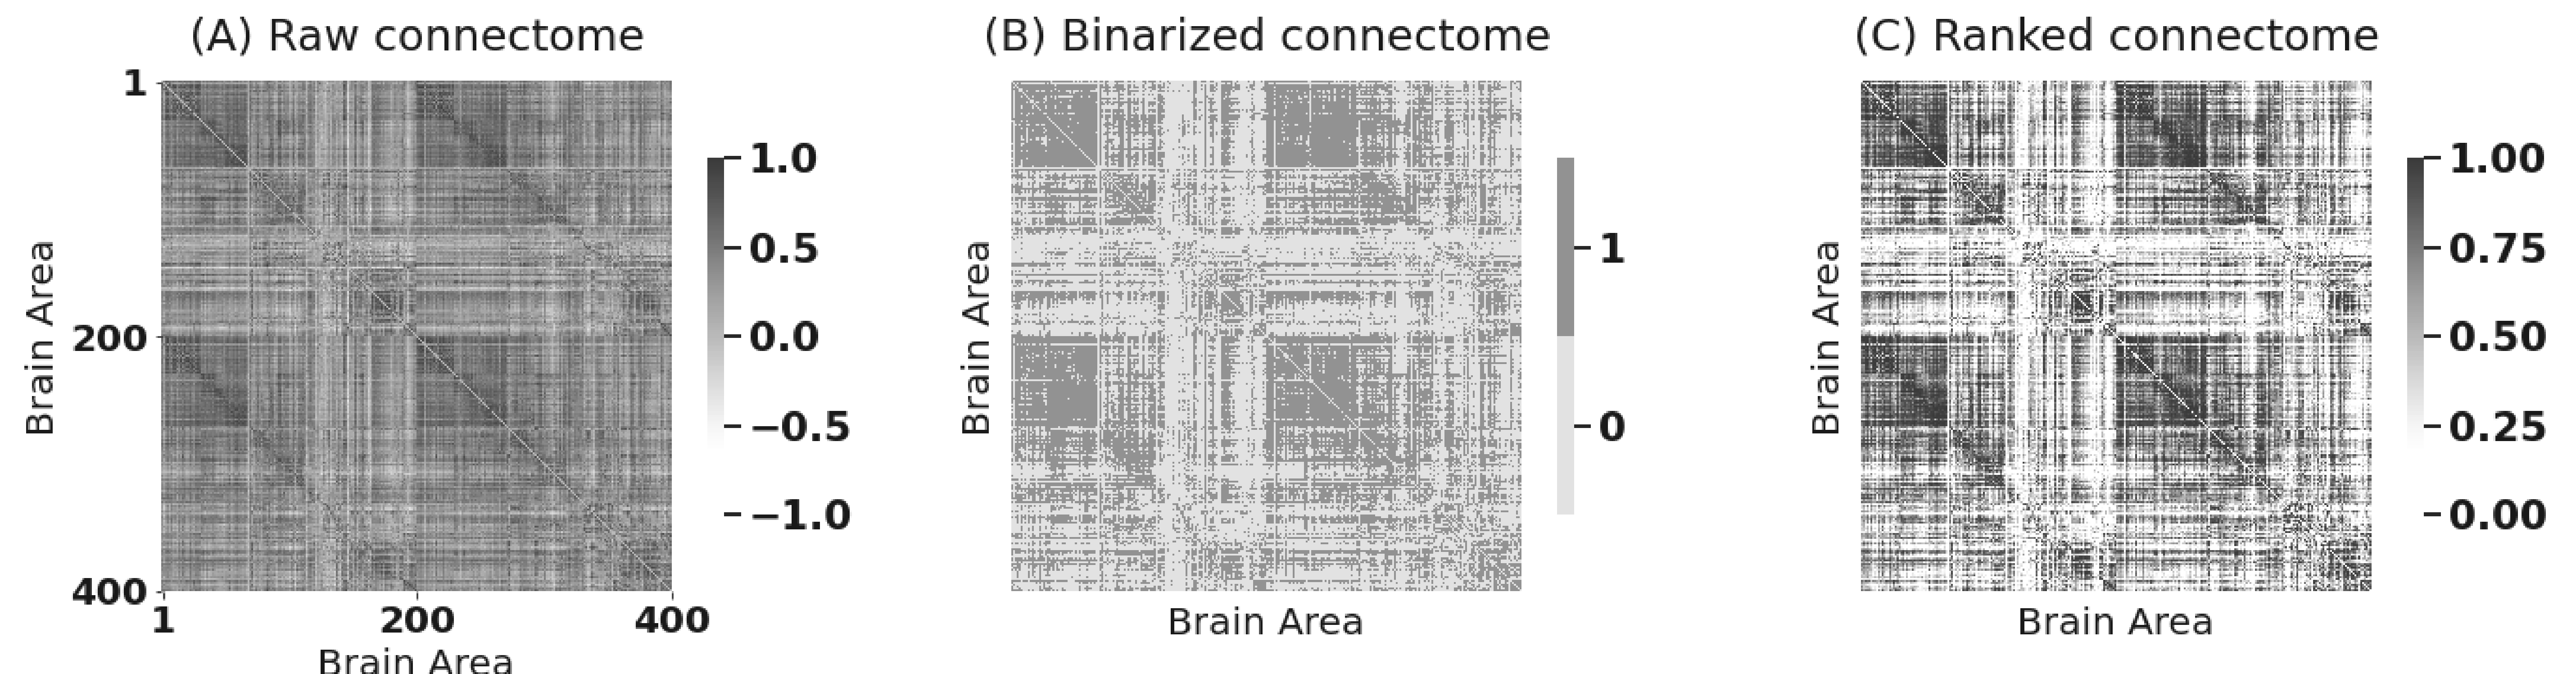
\includegraphics[width=\linewidth]{foundations/ch2/Images/cleaning_connectomes.png}
    \caption[Re-weighting connectome edge-weights]{\textbf{(A)} The cleaned connectome, before re-weighting. \textbf{(B)} The binarized connectome. \textbf{(C)} The ranked connectome.}
    \label{fig:ch2:cleaned_connectomes}
\end{figure}

This has shifted the histogram of edge-weights, as we can see by plotting a histogram:

\begin{lstlisting}[style=python]
import seaborn as sns

fig, ax = plt.subplots(2,1, figsize=(10, 10))
sns.histplot(A_clean[A_clean > 0].flatten(), ax=ax[0]);
ax[0].set_xlabel("Edge weight")
ax[0].set_title("Histogram of human connectome, non-zero edge weights");

sns.histplot(A_ptr[A_ptr > 0].flatten(), ax=ax[1]);
ax[1].set_xlabel("ptr(Edge weight)")
ax[1].set_title("Histogram of human connectome, passed-to-ranks")
\end{lstlisting}
The histograms before and after passing the adjacency matrix to ranks are shown in Figure \ref{fig:ch2:ptrhists}.

\begin{figure}[h]
    \centering
    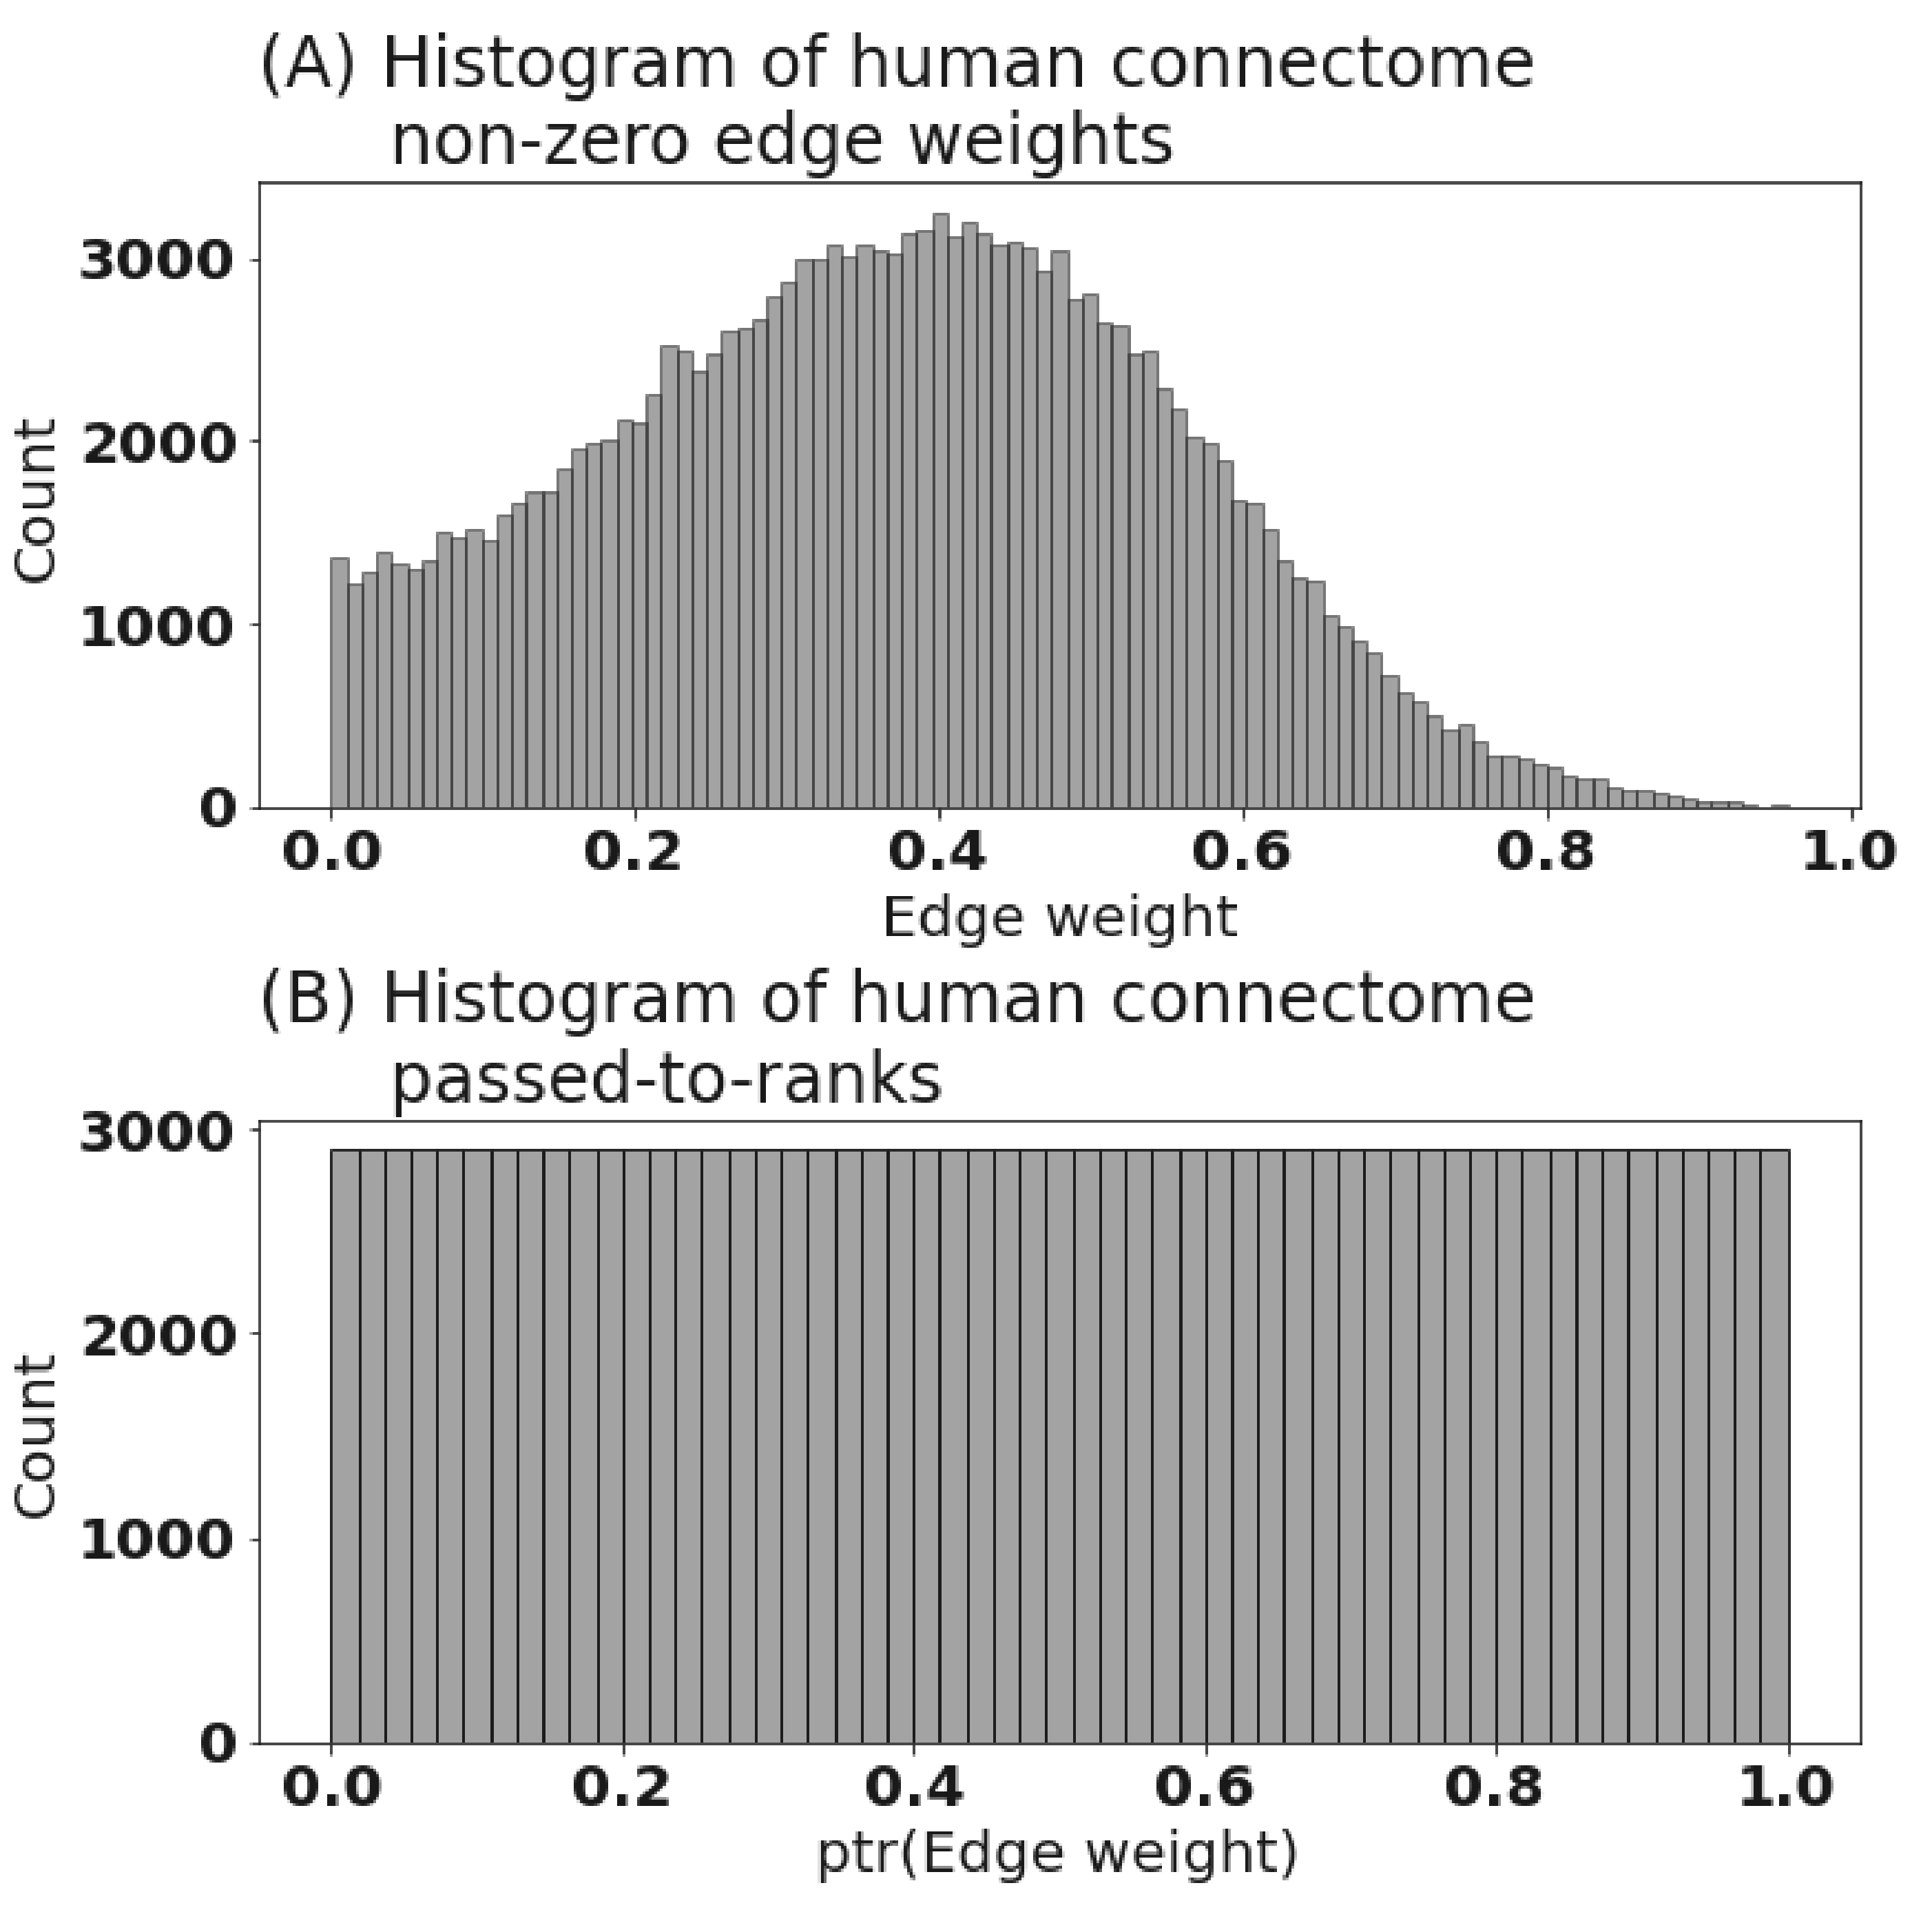
\includegraphics[width=0.6\linewidth]{foundations/ch2/Images/ptrhists.png}
    \caption[Histograms of connectome edge weights]{\textbf{(A)} Histogram of the edge-weights in the adjacency matrix before normalization. \textbf{(B)} Histogram of the edge weights in the adjacency matrix after \texttt{ptr}.}
    \label{fig:ch2:ptrhists}
\end{figure}

This has the desirable property that it bounds the network's edge weights to be between $0$ and $1$, as we can see above, which is often crucial if we seek to compare two or more networks and the edge weights are relative in magnitude (an edge's weight might mean something in relation to another edge's weight in that same network, but an edge's weight means nothing in relation to another edge's weight in a separate network). Further, passing to ranks is not very susceptible to outliers, as we will see in later chapters. 

Again, we will turn the edge-weight transformation step into its own class:

\begin{lstlisting}[style=python]
class FeatureScaler(BaseEstimator, TransformerMixin):
    
    def fit(self, X):
        return self
    
    def transform(self, X):
        print("Scaling edge-weights...")
        A_scaled = pass_to_ranks(X)
        return (A_scaled)
    
feature_scaler = FeatureScaler()
A_cleaned_scaled = feature_scaler.transform(A_clean)
# Scaling edge-weights...
\end{lstlisting}

\subsubsection*{Transformation pipelines}

As you can see, there are a number of data transformations that need to be executed to prepare network data for machine learning algorithms. One thing that might be desirable is to develop a pipeline which automates the data preparation process for you. We perform this using the \texttt{Pipeline} class from \texttt{sklearn}. The \texttt{Pipeline} class can help us apply sequences of transformations. Here is a simple pipeline for doing all of the steps we have performed so far:
\begin{lstlisting}[style=python]
from sklearn.pipeline import Pipeline

num_pipeline = Pipeline([
    ('cleaner', CleanData()),
    ('scaler', FeatureScaler()),
])

A_xfm = num_pipeline.fit_transform(A)
# Cleaning data...
# Purging 0 nodes...
# Scaling edge-weights..
\end{lstlisting}

The pipeline class takes a list of name/estimator pairs defining a sequence of steps. All but the last estimator must be transformers, which implement the \texttt{fit\_transform()} method. In our case, this is handled directly by the \texttt{TransformerMixin} base class.

When you call the \texttt{fit\_transform()} method of the numerical pipeline, it calls the \texttt{fit\_transform()} method on each of the transformers, and passes the output of each call as the parameter to the next call, until it reaches the final estimator, for which it just calls the \texttt{fit()} method. 

Next, we'll see the real handiness of the \texttt{Pipeline} module. The reason we went to lengths to define a pipeline was that we wanted to have an easily reproducible procedure that we could efficiently apply to new connectomes. This is easy to apply to the second subject in our dataset:

\begin{lstlisting}[style=python]
A_xfm2 = num_pipeline.fit_transform(As[1])
# Cleaning data...
# Purging 0 nodes...
# Scaling edge-weights...
\end{lstlisting}

\newpage
\section{Selecting and training a network machine learning model}
\label{sec:ch2:select}

So, now you've got your data loaded and pre-processed... what next?

\subsection{Generating new representations from your data}

As you were briefly introduced to in Section \ref{sec:ch1:whatis} and will cover more thoroughly in Chapter \ref{sec:ch6}, a major problem with learning from network data is that, inherently, networks in their rawest form are not tabular datasets. This means that if you want to apply any of the breadth of knowledge that has been acquired in general machine learning (which is typically designed for tabular datasets), you need to learn how to adapt your network to be compatible with tabular approaches, or learn how to adapt your general machine learning architecture for network layouts, such as adjacency matrices, which properly convey the dependences in network data. This is called \emph{representation learning}, and even neural networks typically do this under the hood with architectures like autoencoders.

As you will learn, particularly in the end of this book in Chapter \ref{sec:ch10}, the former is possible, but generally a bit more involved. The latter approach tends to be, in our opinion, a bit more straightforward at first, and is usually fantastic for most applications. So, how do you obtain a tabular representation of your dataset? 

Well, one possible thing you can do is you can use something called a spectral embedding from Chapter \ref{sec:ch6}, a technique that you will learn has a wide range of applications in network machine learning whether you are studying one network, pairs of networks, or multiple networks. Let's see what happens when we spectrally embed our connectome:

\begin{lstlisting}[style=python]
from graspologic.embed import AdjacencySpectralEmbed

embedding = AdjacencySpectralEmbed().fit_transform(A_xfm)
\end{lstlisting}

An \emph{embedding} takes the adjacency matrix, which is a matrix representation of the entire network, and turns it into a tabular array. Each row is called an \emph{estimated latent position} for a given node, and each column is called an \emph{estimated latent dimension} of the network. This means that if there are $n$ nodes, there are $n$ rows of the spectral embedding, and if there are $d$ estimated latent dimensions of the network, there are $d$ columns. Overall, the spectral embedding has taken the $n \times n$ adjacency matrix, which we \emph{can't} inherently use network machine learning algorithms on, and \emph{transformed} it into a $n \times d$ tabular array, which we \emph{can} inherently use machine learning algorithms on. We'll visualize this embedding using a \emph{pairs plot}, which as you will learn later, is a scatter plot showing where each node is a single point in the plot, and the x and y axes are different \emph{pairs} of latent dimensions for that particular node:

\begin{lstlisting}[style=python]
from graspologic.plot import pairplot

_ = pairplot(embedding, title="Spectral Embedding for connectome")
\end{lstlisting}
The results of this pairs plot are shown in Figure \ref{fig:ch2:pairplots}(A).

As it turns out, this particular representation of the adjacency matrix through the \emph{spectral embedding} can, optionally, be tied into a statistical model if you make some assumptions; particularly, those of the stochastic block model described in Section \ref{sec:ch5:sbm}. Basically, the stochastic block model says that each node is a member of a subgroup, called a \emph{community}, and its connectivity to other nodes in the network is dictated by which community it is a member of, and which community the other node is a member of. This sounds a \emph{lot} like the question that your colleague wanted you to approach, since he wanted a way to take the nodes of the network and form ``functionally similar'' subgroups from them. 

\subsection{Using your representations to learn new features from the network}

Now that we have a tabular representation of the data, we can take attempt to use the intuition and assumptions of the stochastic block model to cluster our nodes. Let's see what happens when we apply \texttt{KMeans} to our data:
\begin{lstlisting}[style=python]
from sklearn.cluster import KMeans

labels = KMeans(n_clusters=2).fit_predict(embedding)
_ = pairplot(embedding, labels=labels, legend_name="Predicter Clusters", 
                 title="KMeans clustering")
\end{lstlisting}

The results of this pairs plot are shown in Figure \ref{fig:ch2:pairplots}(B).
\begin{figure}
    \centering
    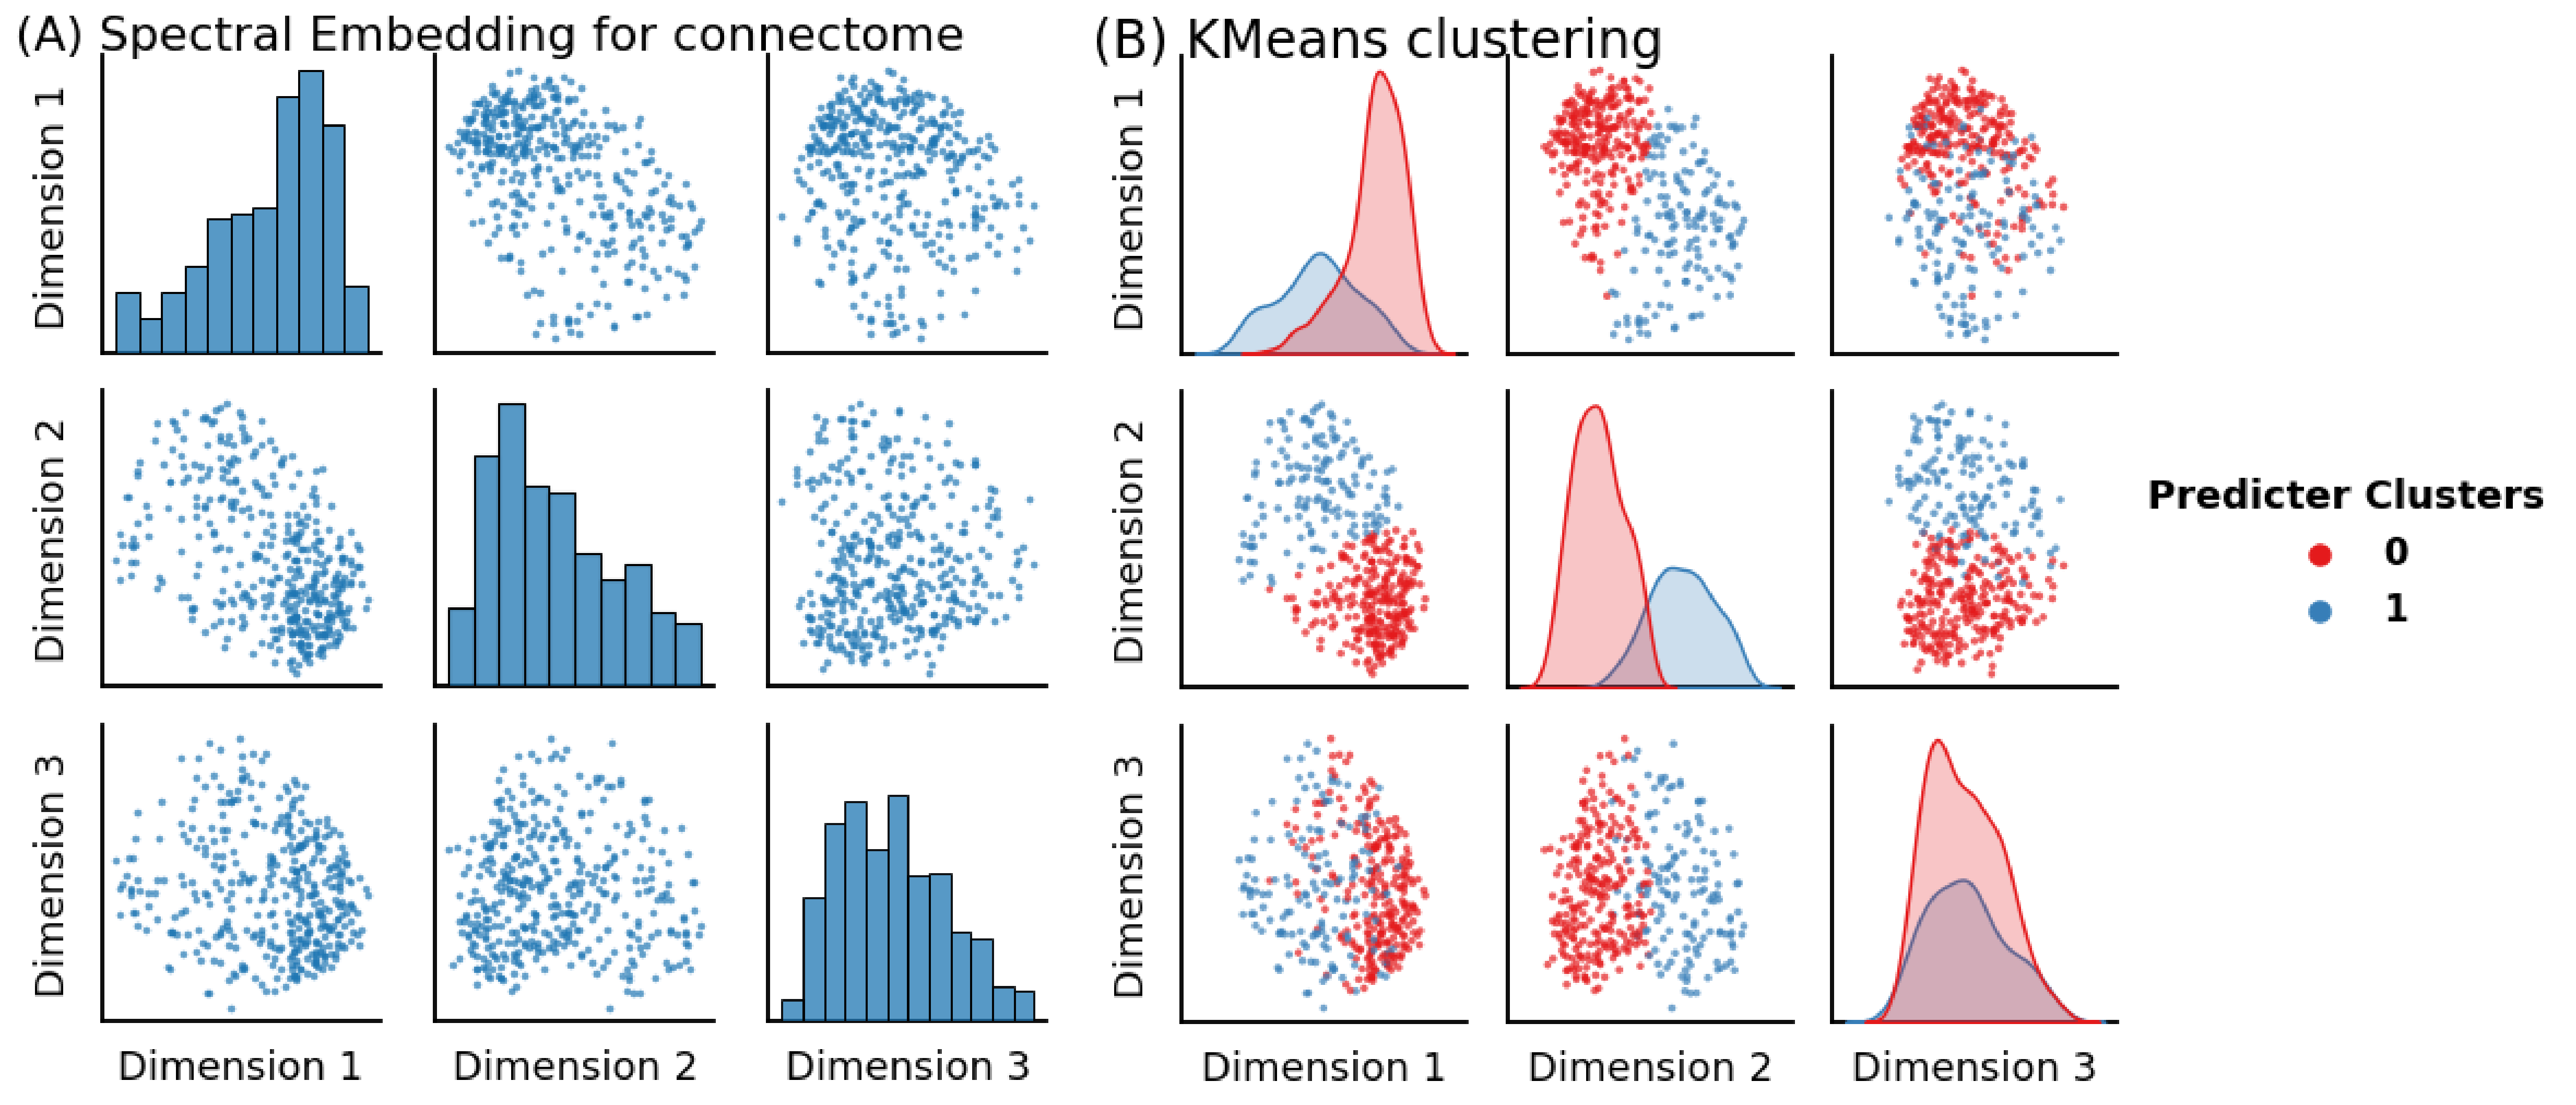
\includegraphics[width=\linewidth]{foundations/ch2/Images/pairplots.png}
    \caption[The pairs plot for embedded connectomes]{\textbf{(A)} shows the  pairs plot for the estimated latent dimensions. \textbf{(B)} shows the  pairs plot with predicted communities of nodes via \texttt{KMeans} with $2$ clusters.}
    \label{fig:ch2:pairplots}
\end{figure}
So, it looks like the $k$-means was able to learn $2$ clusters from our dataset. These clusters are indicated by the ``blobs'' of points that are red or blue, respectively.

If you're careful, you'll notice we did something a little weird here. Why did we choose $2$? Why not $5$? Why not $8$? We chose $2$ here somewhat arbitrarily. In general, when you don't know what to expect from your data (we didn't know what to expect here, other than that we wanted a modestly sized way to group the nodes up), it's a good idea to use quantitative means to make these determinations for you. 

With \texttt{KMeans}, we can use something called the silhouette score to do this for us. You choose the optimal number of clusters as the clustering with the highest silhouette score. You'll learn a lot more about the silhouette score when you learn about community detection in Section \ref{sec:ch7:comm_detect}. \texttt{graspologic} makes this process pretty straightforward with a \texttt{KMeansCluster} class, which uses the silhouette score under the hood:

\begin{lstlisting}[style=python]
from graspologic.cluster import KMeansCluster

labels = KMeansCluster(max_clusters=10).fit_predict(embedding)
_ = pairplot(embedding, labels=labels, title="KMeans clustering, automatic selection", 
                 legend_name="Predicted Clusters")
\end{lstlisting}
Unlike the previous approach, it looks like with silhouette score selection, we ended up with $5$ clusters being optimal, not $2$. The pairs plot for the embedded data with the new labels are in Figure \ref{fig:ch2:pairplots_impute}(A). Note that you might get a different number of estimated clusters than we did, because there is some randomness in the unsupervised learning procedure that we used here.

So, what about other possible approaches? Unless you are pretty confident that the clusters you are looking for have ``blobs'' that are totally spherically symmetric (basically, they look like ``balls'' in the dataset), $k$-means can be a pretty bad idea. As you'll learn later, another strategy called the gaussian mixture model, or \texttt{GMM}, handles this a bit more elegantly, and allows your cluster blobs to be pretty much any ellipse-like shape. We can use \texttt{GMM} and automatically select the number of clusters using the Bayesian Information Criterion, or BIC, with \texttt{AutoGMMCluster}:
\begin{lstlisting}[style=python]
from graspologic.cluster import AutoGMMCluster

labels = AutoGMMCluster(max_components=10).fit_predict(embedding)
_ = pairplot(embedding, labels=labels, title="AutoGMM Clustering", 
                  legend_name="Predicted Clusters")
\end{lstlisting}
The pairs plot for the embedded data with the labels determined by \texttt{GMM} in Figure \ref{fig:ch2:pairplots_impute}(B). It looks like GMM actually found $4$ clusters to be a bit more optimal than $3$ clusters. 

\begin{figure}
    \centering
    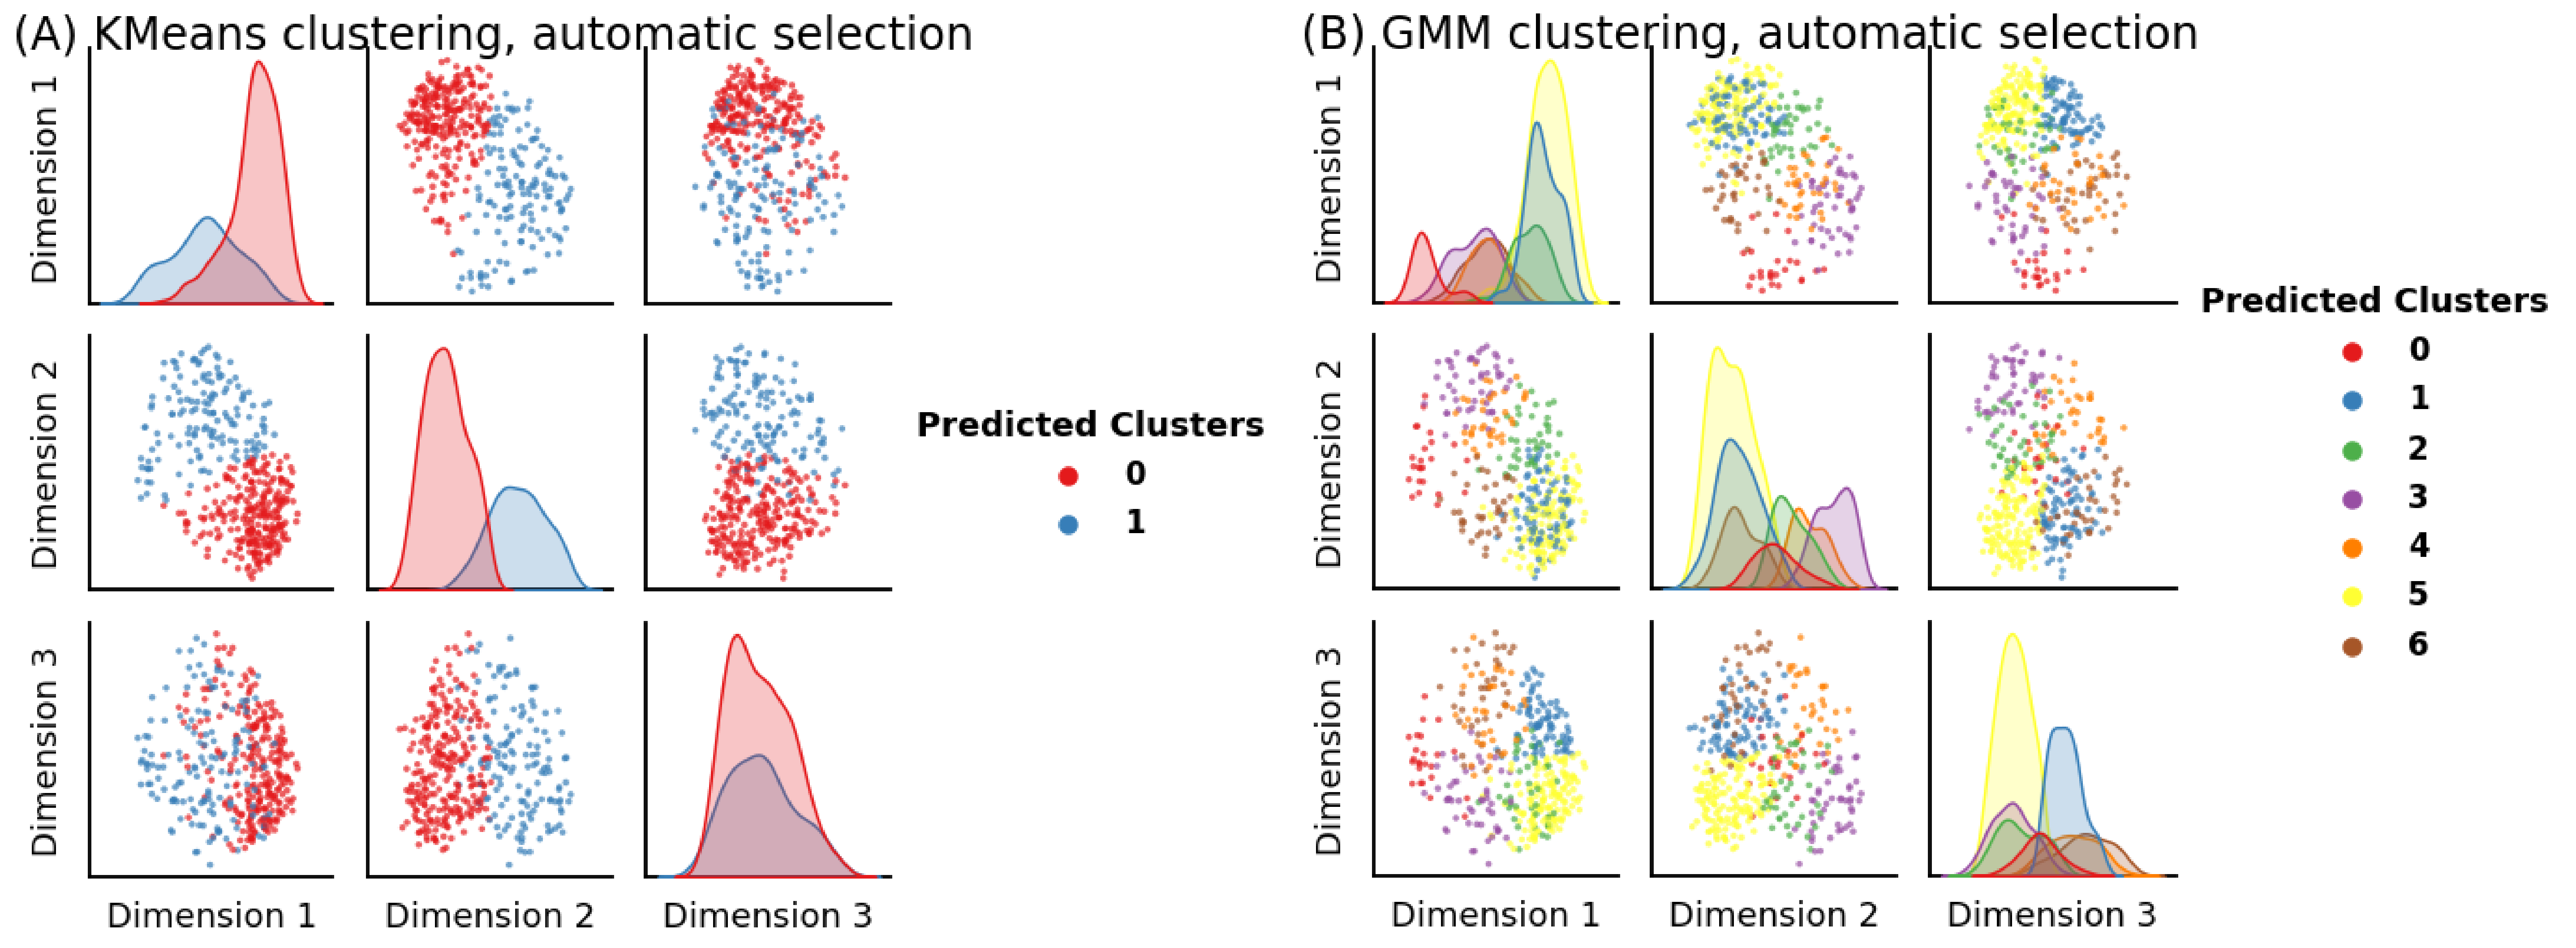
\includegraphics[width=\linewidth]{foundations/ch2/Images/pairplots_impute.png}
    \caption[Comparison of labels estimated by $k$-means and GMM]{\textbf{(A)} the pairs plot for the embedded data, with node communities estimated by \texttt{KMeans}. \textbf{(B)} the pairs plot for the embedded data, with node communities estimated by \texttt{GMM}.}
    \label{fig:ch2:pairplots_impute}
\end{figure}

\newpage
\section{Fine tuning a network machine learning model}
\label{sec:ch2:finetune}

Now that we have figured out an appropriate way to represent our network, and we've gained a few insights, it's time to tune things up a little bit.

In \ref{sec:ch2:select} we saw how to take one of the networks and use embeddings combined with various clustering techniques to learn about latent structure in the data.

However, there's a big caveat: your colleague sent you over a hundred networks, and you ignored all but one of them! Surely, there's something that you can learn from all of them, right?

Fortunately, when you have a multiple network problem, there are plenty of approaches that you can use to learn from all of them simultaneously. Let's break down how we can approach this.

You want to produce a representation of all of your networks. These networks all have the same nodes, which are the different areas of the brain. For all intents and purposes, you can assume that these different nodes mean the same thing across all of the different people, even if they are different based on each individual. What you want to learn is whether there is some {shared} structure across all of the different networks present in the nodes. To do this, you are going to want to be able to take {all} of your networks, and produce an embedding in which you can look at each {node} as its own object. Does anything exist to help you?

There sure does. A particular representation called \texttt{MASE} from Section \ref{ch6:multinet:mase} does just this. It allows you to take many networks, and learn a single representation for the nodes across all of the networks. This representation, in particular, is going to effectively {borrow strength} from all of the networks you pass in, so you won't have to worry about whether you are just ignoring all of the networks but one like you did before. Let's see what \texttt{MASE} can do for us here:


\begin{lstlisting}[style=python]
from graspologic.embed import MultipleASE

embedding = MultipleASE().fit_transform(As)
_ = pairplot(embedding, title="Multiple spectral embedding of all connectomes")
\end{lstlisting}

Let's take a look at what happens when we apply our clustering to this embedding:

\begin{lstlisting}[style=python]
labels = AutoGMMCluster(max_components=10).fit_predict(embedding)
_ = pairplot(embedding, labels=labels,
                title="Multiple spectral embedding of all connectomes", 
                legend_name="Predicted Clusters")
\end{lstlisting}
The pairs plot of the \texttt{MASE} embedding with labels estimated by \texttt{GMM} is shown in Figure \ref{fig:ch2:mase}. Again, the clustering algorithm applied has some element of randomness to it, so don't be concerned if you don't get the exact same number of predicted clusters as we did, or if your clusters look a little different.

\begin{figure}[h]
    \centering
    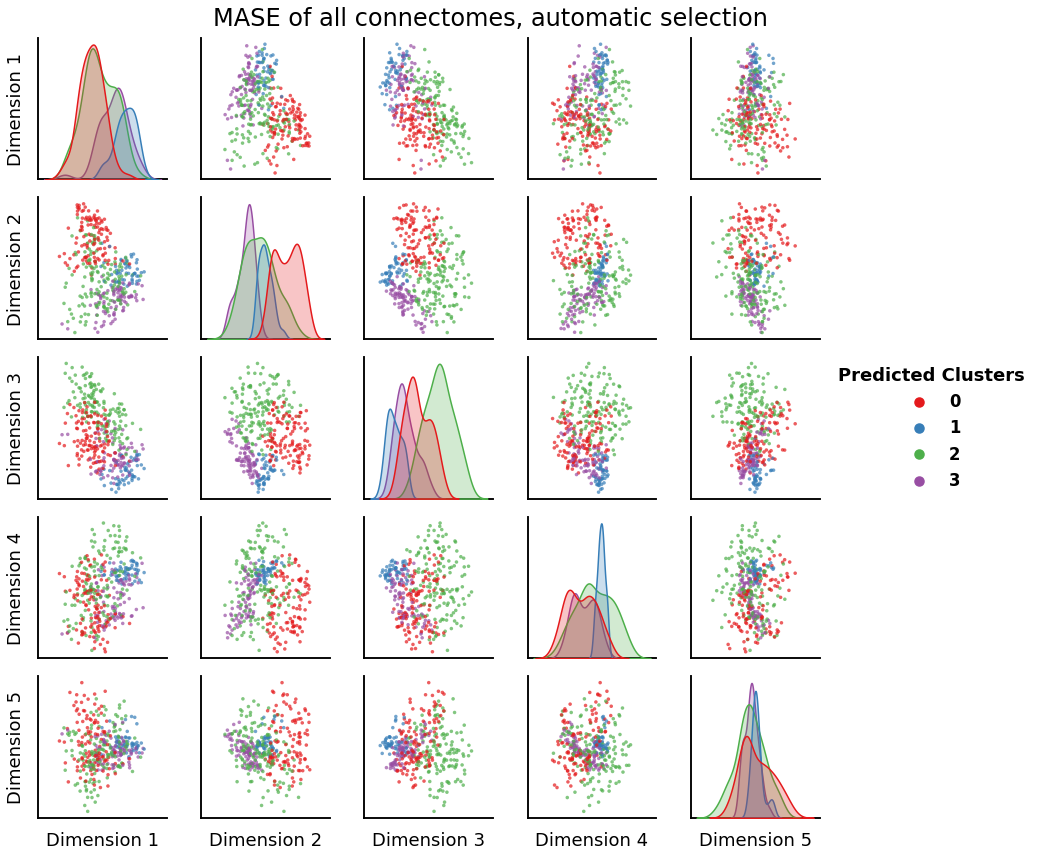
\includegraphics[width=\linewidth]{foundations/ch2/Images/mase.png}
    \caption[Joint embedding with estimated labels for connectomes]{\textbf{(A)} The \texttt{MASE} embedding, which learns an embedding across all networks in your dataset. \textbf{(B)} The \texttt{MASE} embedding, with labels learned by \texttt{GMM}.}
    \label{fig:ch2:mase}
\end{figure}
\newpage
\section{Discover and visualize the system to gain insights}
\label{sec:ch2:discover}

So, now we've got a codebase accumulated to read in the input data, get it cleaned up, embed it while borrowing strength from all networks, and make some predictions. 

So, now we're finished, right?

Wrong! The end of a computational analysis typically means the fun is just beginning: it's now time to \emph{make sense} of whatever, exactly, it is that you just did!

How could we visualize the node clusters (or, more formally, called \emph{communities}) that we just made? We already known about the pairs plot, which we saw in Figure \ref{fig:ch2:mase}(B). 

What if we take a look at the nodes, which if we remember were areas of the brain, and visualize how they \emph{really} look in the brain's natural space?

It turns out that the areas of the brain corresponding to the nodes in your network are, in fact, \emph{known} 3D points in the brain. This means that, with some minor work, we can figure out the coordinates of the individual nodes for the brain. Let's use the neuroparc repository from \cite{Lawrence2021Mar} to grab the 3D coordinates of each node in the network. You don't need to worry too much about how this code works; at a high-level, it just obtains 3D coordinates for the nodes of the network in a \texttt{json} file, and then parses them into a \texttt{pandas} dataframe:


\begin{lstlisting}[style=python]
from urllib import request
import json
import pandas as pd

coord_dest = os.path.join(FMRI_PATH, "coordinates.json")
request.urlretrieve("https://github.com/neurodata/neuroparc/" + "raw/master/atlases/label/Human/Metadata-json/" + parcellation + "_space-MNI152NLin6_res-2x2x2.json", coord_dest);

with open(coord_dest) as coord_f:
    coords = []
    for roiname, contents in json.load(coord_f)["rois"].items():
        try:
            if roiname != "0":
                coord_roi = {"x" : contents["center"][0], "y" : contents["center"][1], "z" : contents["center"][2]}
                coords.append(coord_roi)
        except:
            continue
            
coords_df = pd.DataFrame(coords)
\end{lstlisting}

Now that we have the coordinates, let's try plotting the nodes, but in their native spatial orientation. Here, the color will indicate the predicted label, from our clustering. The slices we'll show will be a saggital slice through the brain. A saggital slice shows the brain nodes oriented from back (right of the plot) of the brain to front (left of the plot), and from bottom (bottom of the plot) to top (top of the plot). On the left, we show the brain with the lobe annotations, and on the right, the predicted labels of each node in color, where each node is shown in its true physical location:

\begin{lstlisting}[style=python]
import matplotlib.image as mpimg

coords_df["Community"] = labels
coords_df['Community'] = coords_df['Community'].astype('category')
fig, axs = plt.subplots(1, 2, figsize=(18, 6))
axs[0].imshow(mpimg.imread('./Images/lobes.png'))
axs[0].set_axis_off()
sns.scatterplot(x="y", y="z", data=coords_df, hue="Community", ax=axs[1])
\end{lstlisting}
\begin{figure}[h]
    \centering
    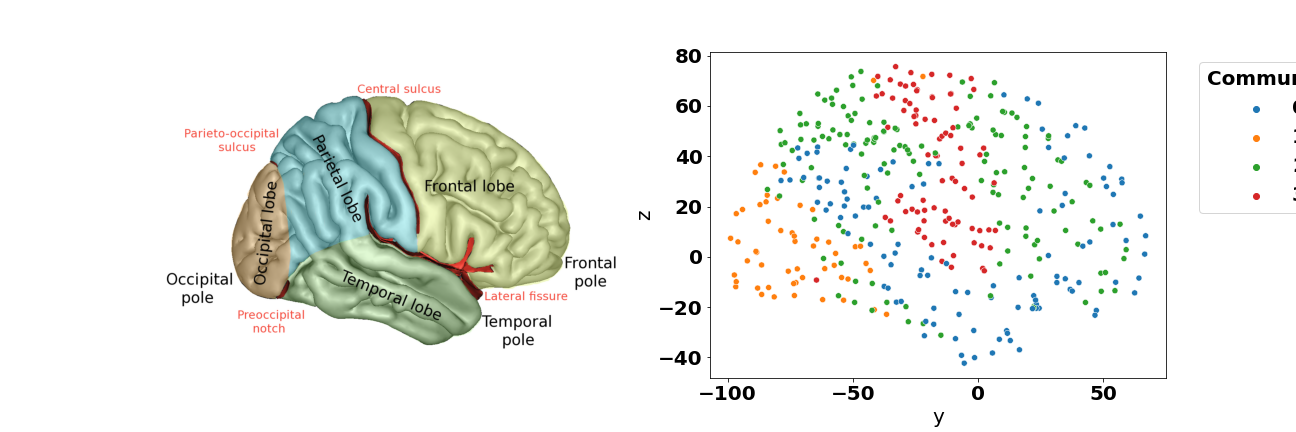
\includegraphics[width=\linewidth]{foundations/ch2/Images/brain_preds.png}
    \caption[Visualizing estimated node communities in 3D space]{Visualizing the estimated node communities with brain lobe annotations.}
    \label{fig:ch2:brain_preds}
\end{figure}

The resulting plot is shown in Figure \ref{fig:ch2:brain_preds}. So, the estimated communities of each node don't quite perfectly align with the brain lobe that the node is in. However, nodes in the tend to be \emph{spatially close} to other nodes in the same estimated community. Notice, for instance, that a lot of nodes in the left side of the brain, the part marked ``occipital lobe'' in the plot, tend to be the same color. In our plot, these nodes are orange; in your plot, they might be a different color. 

In neuroimaging, there tend to be ``groups'' of brain areas that work together, which are organized in files called ``parcellations''. The idea is that they ``parcellate'' (segment) different areas of the brain baesd on two factors: whether the areas of the brain work together, and whether they are located near each other in the brain. Let's see how well the labels we obtained align with these parcellations. We'll do this by looking at the different parcellations (there are $7$ of them in the one that we will use here), and count the number of nodes in a given community (the thing that you just estimated, indicated by color, above) that are assigned to a particular parcel as well. This means that we will end up with a matrix where the number of rows are the number of true parcels in the brain, the number of columns is the number of predicted communities that you found above, and the entries of the matrix are the counts of nodes in the network that are assigned to a given community \emph{and} fall into a given parcel:

\begin{lstlisting}[style=python]
import contextlib
import datasets.dice as dice
from sklearn.metrics import confusion_matrix
from graphbook_code import cmaps

group_dest = os.path.join("./datasets/", "Yeo-7_space-MNI152NLin6_res-2x2x2.nii.gz")
request.urlretrieve("https://github.com/neurodata/neuroparc/" + "blob/master/atlases/label/Human/" +
"Yeo-7_space-MNI152NLin6_res-2x2x2.nii.gz?raw=true", group_dest);
roi_dest = os.path.join("./datasets/", "Schaefer200_space-MNI152NLin6_res-2x2x2.nii.gz")
request.urlretrieve("https://github.com/neurodata/neuroparc/" + "blob/master/atlases/label/Human/" + "Schaefer400_space-MNI152NLin6_res-2x2x2.nii.gz?raw=true", roi_dest);

dicemap, _, _ = dice.dice_roi("./datasets/", "./datasets", "Yeo-7_space-MNI152NLin6_res-2x2x2.nii.gz", 
              "Schaefer200_space-MNI152NLin6_res-2x2x2.nii.gz", verbose=False, plot=False)
actual_cluster = np.argmax(dicemap, axis=0)[1:] - 1

# make confusion matrix
cf_matrix = confusion_matrix(actual_cluster, labels)

# and plot it
ax = sns.heatmap(cf_matrix, cmap=cmaps["sequential"])
ax.set_title("Confusion matrix")
ax.set_ylabel("True Label")
ax.set_xlabel("Predicted Label")
\end{lstlisting}

\begin{figure}[h]
    \centering
    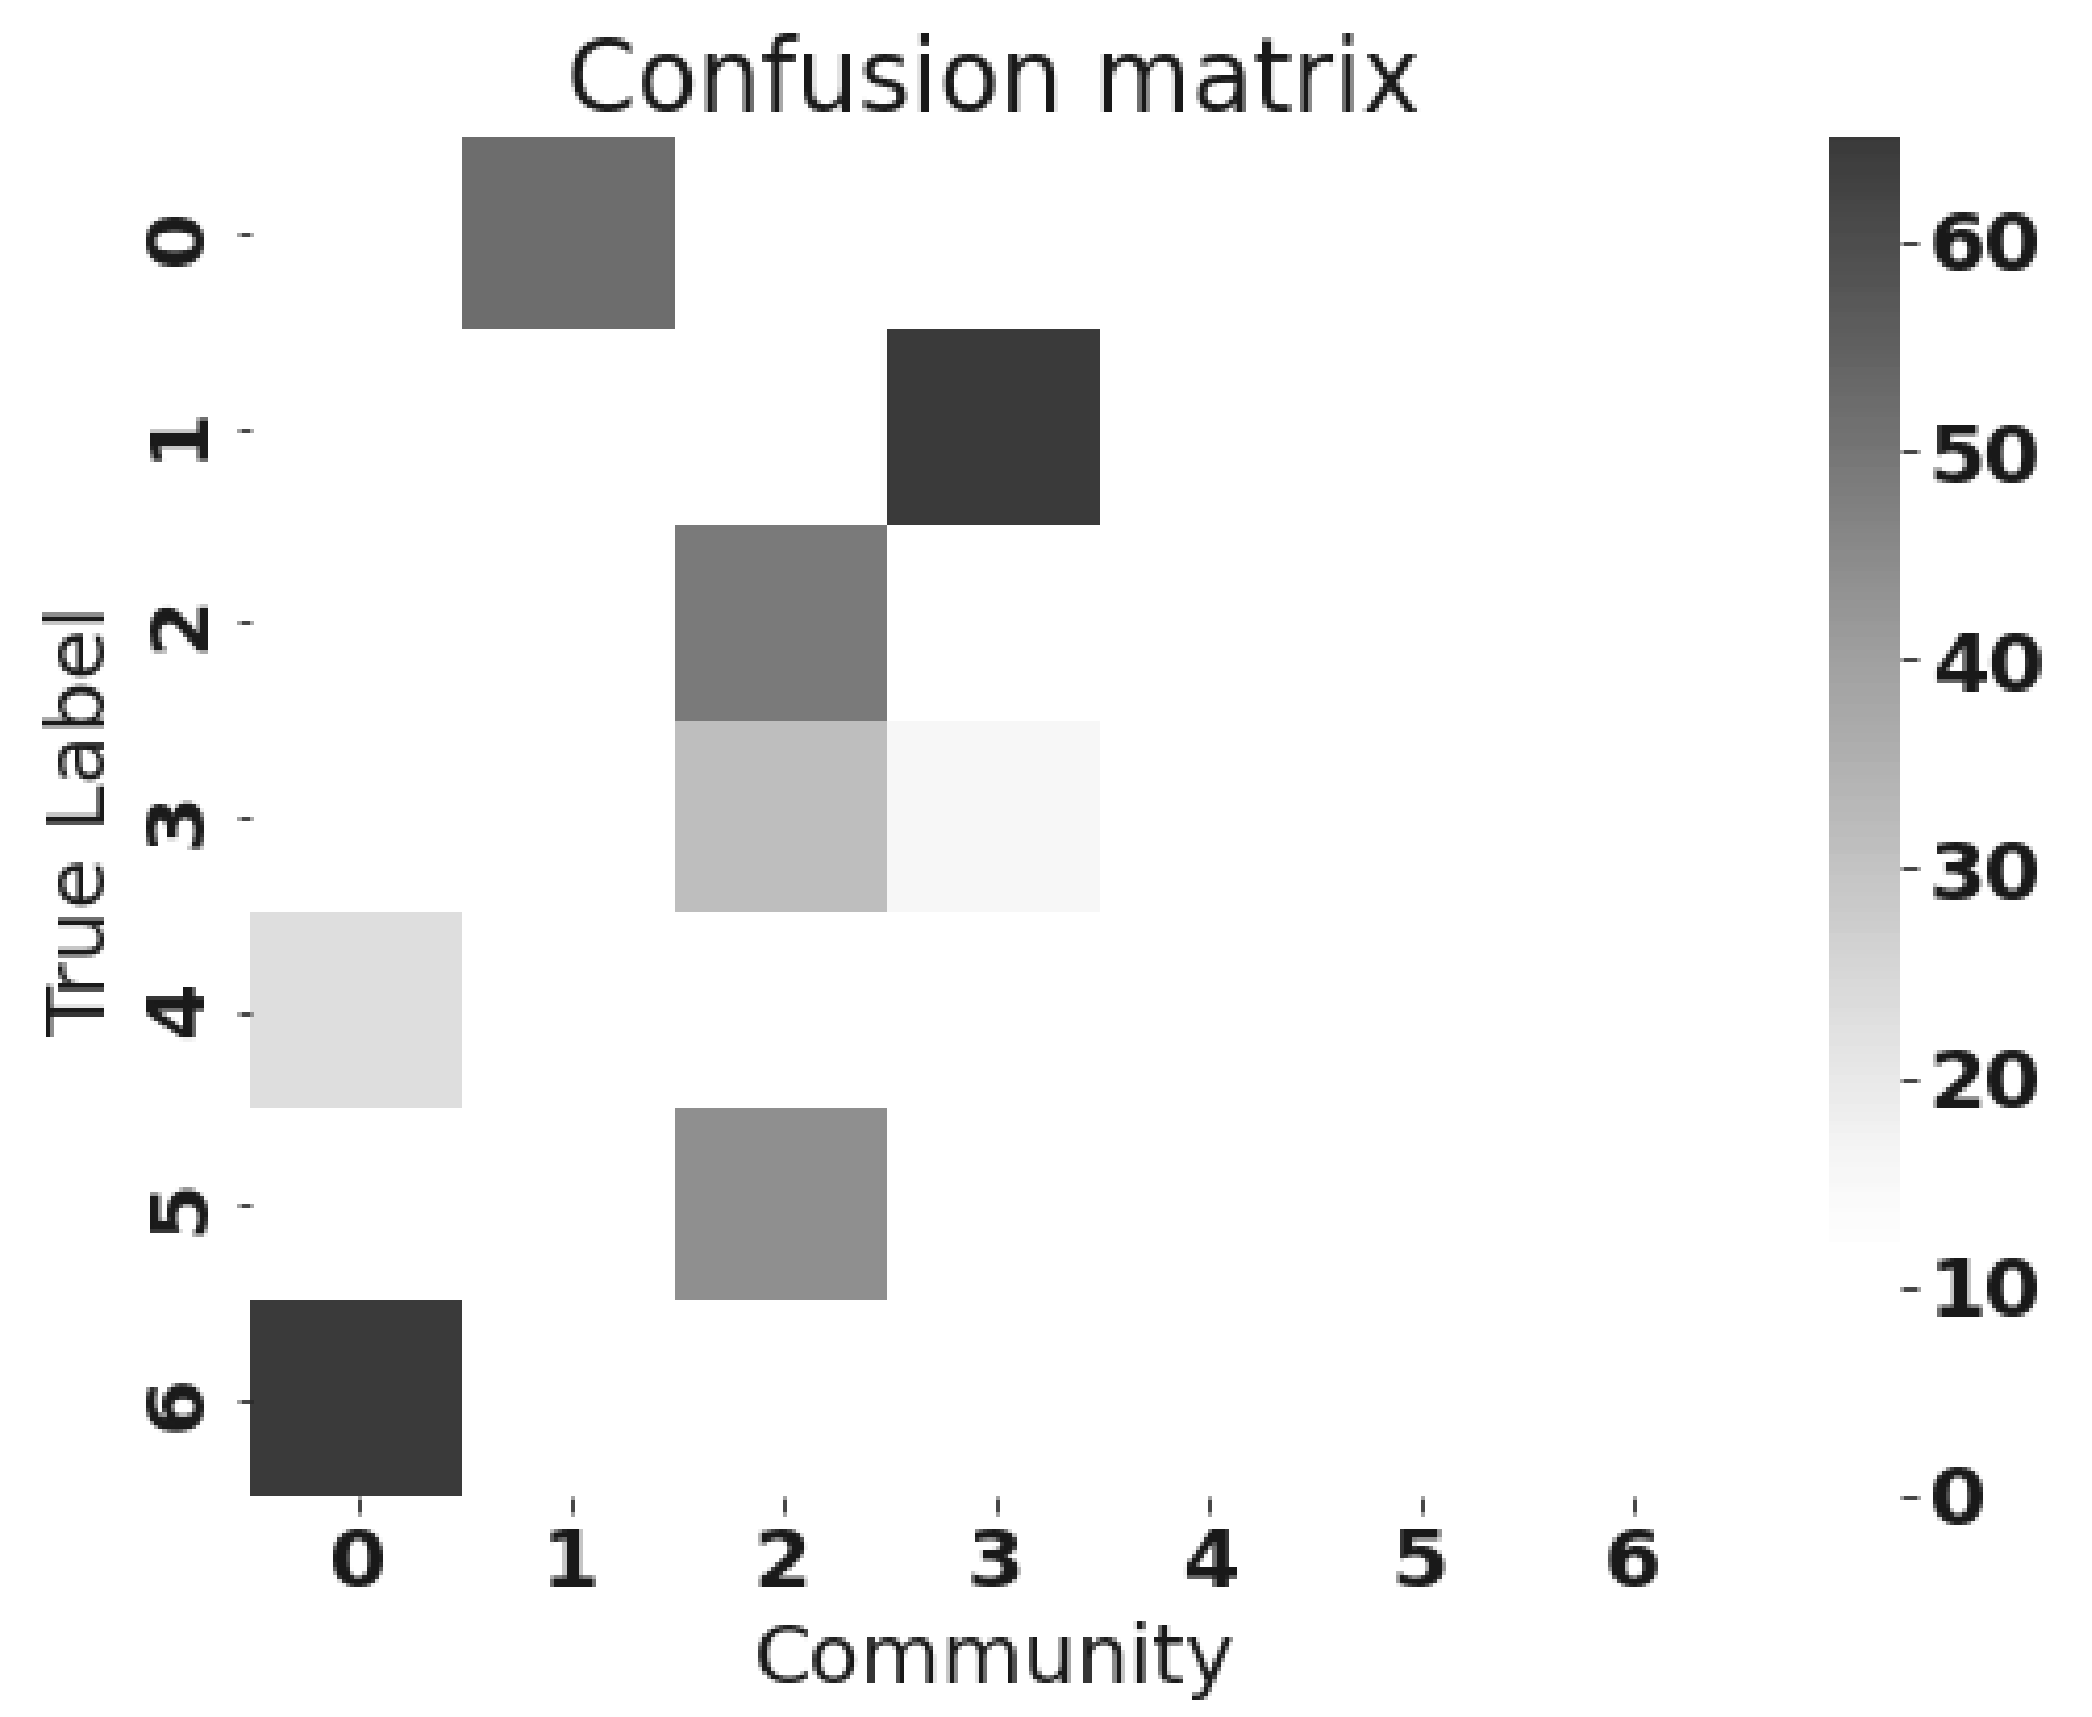
\includegraphics[width=0.5\linewidth]{foundations/ch2/Images/cf_mtx.png}
    \caption[Confusion matrix for node predictions]{The confusion matrix of the estimated clusters for each node in the networks, compared to the lobe that each node is in.}
    \label{fig:ch2:cf_mtx}
\end{figure}
The resulting plot is shown in Figure \ref{fig:ch2:cf_mtx}. in As you will learn in the section on \texttt{MASE} embedding in Section \ref{ch6:multinet:mase}, the mase embedding followed by clustering tends to find groups of nodes that have similar connectivity patterns in the connectomes (it will do a good job at finding the nodes that work together). This means that the nodes in the same community tend to behave ``as a unit'', if you will, in that they tend to be active/inactive together. Basically, what the plot above shows is that nodes that tend to have similar connectivity patterns (from the networks) tend to also be in the same parcel (the \emph{true label}), which makes sense since the parcels are based on connectivity profiles from brains. The clustering isn't \emph{perfect}, in that it is never the case that a single predicted label corresponds to \emph{exactly} one true label. If that were the case, we would expect for each column in the above ``confusion matrix'' to only have one possible true label that nodes within this predicted label are assigned to, which isn't quite the case. 

Taking these conclusions together, we find that some areas of the brain (such as the occipital and parietal areas) feature nodes which are both functionally \emph{and} spatially similar: they tend to show similar connectivity patterns with respect to other groups of nodes in the network, \emph{and} are in similar spatial positions in the brain. On the other hand, for other areas of the brain, while the nodes may be functionally similar, they might not necessarily be spatially similar. This is where the domain expertise kicks in: we don't know how to interpret this particular aspect of our finding, but maybe you or your colleagues do!

Further, while this analysis \emph{only} really ended up looking at whether different groups of nodes worked together, there's really no reason we couldn't \emph{also} incorporate spatial information about the nodes into our analysis. In Section \ref{ch6:joint}, you will learn some techniques for incorporating both the network data itself and other information about the nodes into your analysis through a technique called Covariate-Assisted Spectral Embedding (\texttt{CASE}), such as spatial information.

And this is where the fun of network machine learning comes into play: it is a tool not only to \emph{apply} algorithms to data, but to facilitate \emph{learning new things} about that data as well. You might get some predictable conclusions (such as some of the nodes being both functionally and spatially similar), and you might get some unpredictable conclusions (such as some of the nodes being functionally, but \emph{not} spatially, similar). Your ability to understand network machine learning, while crucial, is going to go \emph{hand in hand} with your ability to understand the intricacies of the domain you want to apply network machine learning to. We hope that we can help with the former part; we'll leave the latter to you!

\subsection{Try it out}

Hopefully this chapter gave you a small scale peek at what a network machine learning project looks like, and showed you a brief introduction to some tools you can use to gain novel insights from your network data. While what we did in this chapter was relatively straightforward, the process from obtaining your data to choosing appropriate network machine learning problems can be extremely arduous! In fact, as a network machine learning scientist, you might find that just obtaining your data in a useful form (a network) and cleaning the data to be usable might take an \emph{enormous} chunk of your time!

If you haven't already done so, now is a fantastic time to grab your laptop, select a network dataset you are interested in, and start trying to work through the whole process from A to Z. If you need some pointers, the \texttt{graspologic} package makes several datasets available to you \cite{graspydata}. We'd recommend working through the contents of this book by first using the example data that is presented in the chapter, and then try to apply the techniques to a network dataset of your choosing.

\bibliographystyle{vancouver}
\bibliography{references}

\part{Representations}
\label{p:rep}
\chapter{Mathematical properties of network data}
\label{sec:ch4}


In this section, you'll learn the basics of network-valued data. As you saw in the introduction, for many reasons, network-valued data is fundamentally different from other forms of data, such as tabular data, that are often used in machine learning. Back in Section \ref{sec:ch1:challenges}, we introduced you to a figure which is going to come up repeatedly throughout this book, so that we can contextualize where we are in the process of learning {how to learn} from networks. The figure looked something like this:

\begin{figure}[h]
    \centering
    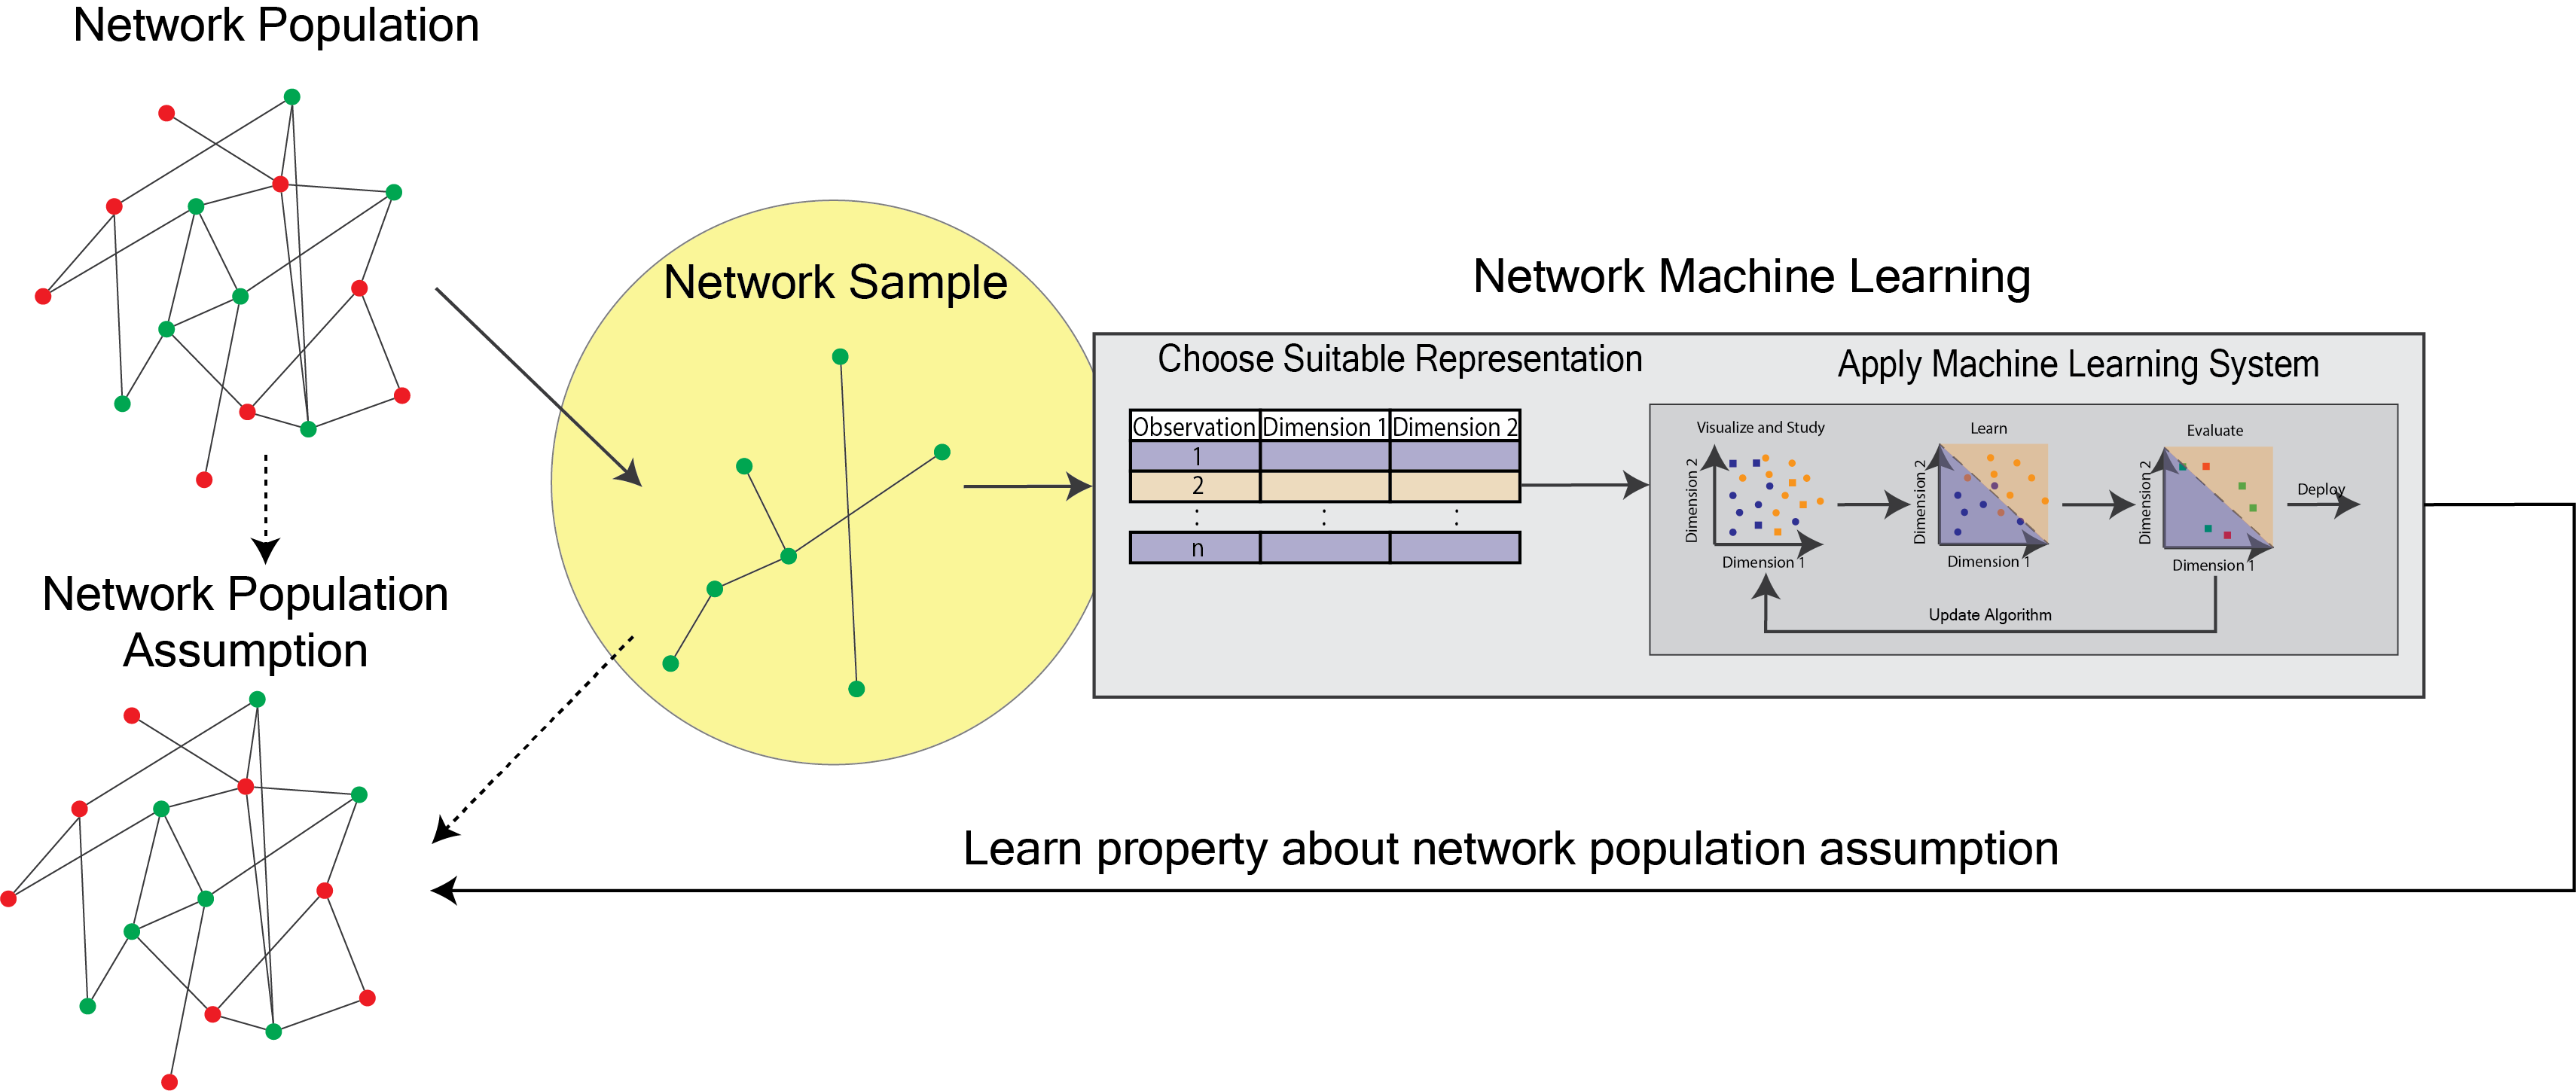
\includegraphics[width=\linewidth]{representations/ch4/Images/network_reps.png}
    \caption[Describing networks schematic]{The statistical learning pipeline. In this chapter, you will learn about how to describe the network you observe in your analysis.}
    \label{fig:ch4:rep_properties}
\end{figure}

When you try to learn from a network that you see through your research, your work, or anywhere else, the first thing to do is to know exactly how to describe that network. This network that you see is known as a {sample} or an {observation} of a network. The reason we call it an \emph{observation} or a \emph{sample} of a network is that the network you see is almost never going to {perfectly} describe the process you are trying to study. It is rarely the case that the network data you obtain will be perfect, as you learned in Section \ref{sec:ch1:challenges}. However, before we start to learn how to characterize that noise and perhaps better describe the observed network, you need to learn how to describe the network you observe first. 

Throughout the subsections, we'll learn about the fundamental representation we use for networks in this book, which is called the adjacency matrix. The reason we turn to adjacency matrices extremely often in network machine learning is that they tend to have nice mathematical properties; particularly, that the matrix is the fundamental unit for \emph{linear algebra}, a subset of mathematics that you might have become introduced to in your mathematical courses. When you apply algorithms to networks, more often than not, you can use \emph{linear algebra} techniques to describe the operation mathematically and in a precise way that allows you to apply the algorithm \emph{en masse} to the entire network.

\newpage 

\section{Matrix representations of networks}
\label{sec:ch4:mtx-rep}

When we work with networks, we need a way to represent them mathematically and in our code. A network itself lives in network space, which is just the set of all possible networks. Network space is kind of abstract and inconvenient if we want to use traditional mathematics, so we'd generally like to represent networks with groups of numbers to make everything more concrete.

More specifically, we would often like to represent networks with \emph{matrices}. In addition to being computationally convenient, using matrices to represent networks lets us bring in a surprising amount of tools from linear algebra and statistics. Programmatically, using matrices also lets us use common \texttt{python} tools for array manipulation like \texttt{numpy}.

For this section, we just wanted to get you acquainted with matrix representations of networks. This section will tie in directly with Section \ref{sec:ch4:prop-net}, so be aware that many of these concepts will be addressed in much more depth as the book progresses.

A common matrix representation of a network is called the Adjacency Matrix, and we'll learn about that first.

\subsection{Adjacency Matrices}

Throughout this book, the beating heart of matrix representations of networks that we will see is the adjacency matrix \cite{Godsil}. The idea is pretty straightforward: Let's say we have a network with $n$ nodes. We give each node an index (usually some value between $1$ and $n$, with one value per node) and then we create an $n \times n$ matrix. If there is an edge between node $i$ and node $j$, we fill the $(i, j)^{th}$ and $(j, i)^{th}$ values of the matrix with an entry, usually $1$ if our network has unweighted edges. In the case of undirected networks, we end up with a symmetric matrix with full of $1$s and $0$s, which completely represents the topology of our network.

Let's see this in action. We'll make a network with only three nodes, since that's small and easy to understand, and then we'll show what it looks like as an adjacency matrix. To visualize this network, we'll use something called a layout plot, provided by \texttt{nx.draw\_network()}.

\begin{lstlisting}[style=python]
import numpy as np
import networkx as nx

G = nx.DiGraph()
# add nodes to the network
G.add_node("1", pos=(1,1))
G.add_node("2", pos=(4,4))
G.add_node("3", pos=(4,2))
# add edges to the network
G.add_edge("1", "2")
G.add_edge("2", "1")
G.add_edge("1", "3")
G.add_edge("3", "1")

# the coordinates in space to use for plotting the nodes
# in the layout plot
pos = {'1': (0, 0), '2': (1, 0), '3': (.5, .5)}

nx.draw_networkx(G, with_labels=True, node_color="tab:purple", pos=pos,
                font_size=10, font_color="whitesmoke", arrows=False, edge_color="black",
                width=1)
\end{lstlisting}

The resulting plot of the network is shown in Figure \ref{fig:ch4:basic_mtxs}(A). Our network has three nodes, labeled $1$, $2$, and $3$. Each of these three nodes is either connected or not connected to each of the two other nodes. We'll make a square matrix $A$, with 3 rows and 3 columns, so that each node has its own row and column associated to it.

So, let's fill out the matrix. We start with the first row, which corresponds to the first node, and move along the columns. If there is an edge between the first node and the node whose index matches the current column, put a $1$ in the current location. If the two nodes aren't connected, add a $0$. When you're done with the first row, move on to the second. Keep going until the whole matrix is filled with $0$'s and $1$'s. 

Since the second and third nodes aren't connected, there is a $0$ in locations $a_{2, 1}$ and $a_{1, 2}$. There are also zeroes along the diagonals, since nodes don't have edges with themselves. In the plot, please take note of how we plotted the adjacency matrix using \texttt{heatmap()}; we won't always show you how to make this plot in the future. 

\begin{lstlisting}[style=python]
from graphbook_code import heatmap
import matplotlib.pyplot as plt
import seaborn as sns

# convert the networkx graph to a numpy array
A = np.asarray(nx.to_numpy_matrix(G))

heatmap(A, annot=True, linewidths=.1, cbar=False, 
        title="Adjacency matrix", xticklabels=[1,2,3], xtitle="Node", 
        yticklabels=[1,2,3], ytitle="Node"
       )


\end{lstlisting}

The resulting adjacency matrix is shown in Figure \ref{fig:ch4:basic_mtxs}(B). Although the adjacency matrix is straightforward and easy to understand, it isn't the only way to represent networks with matrices.

\begin{figure}[h]
    \centering
    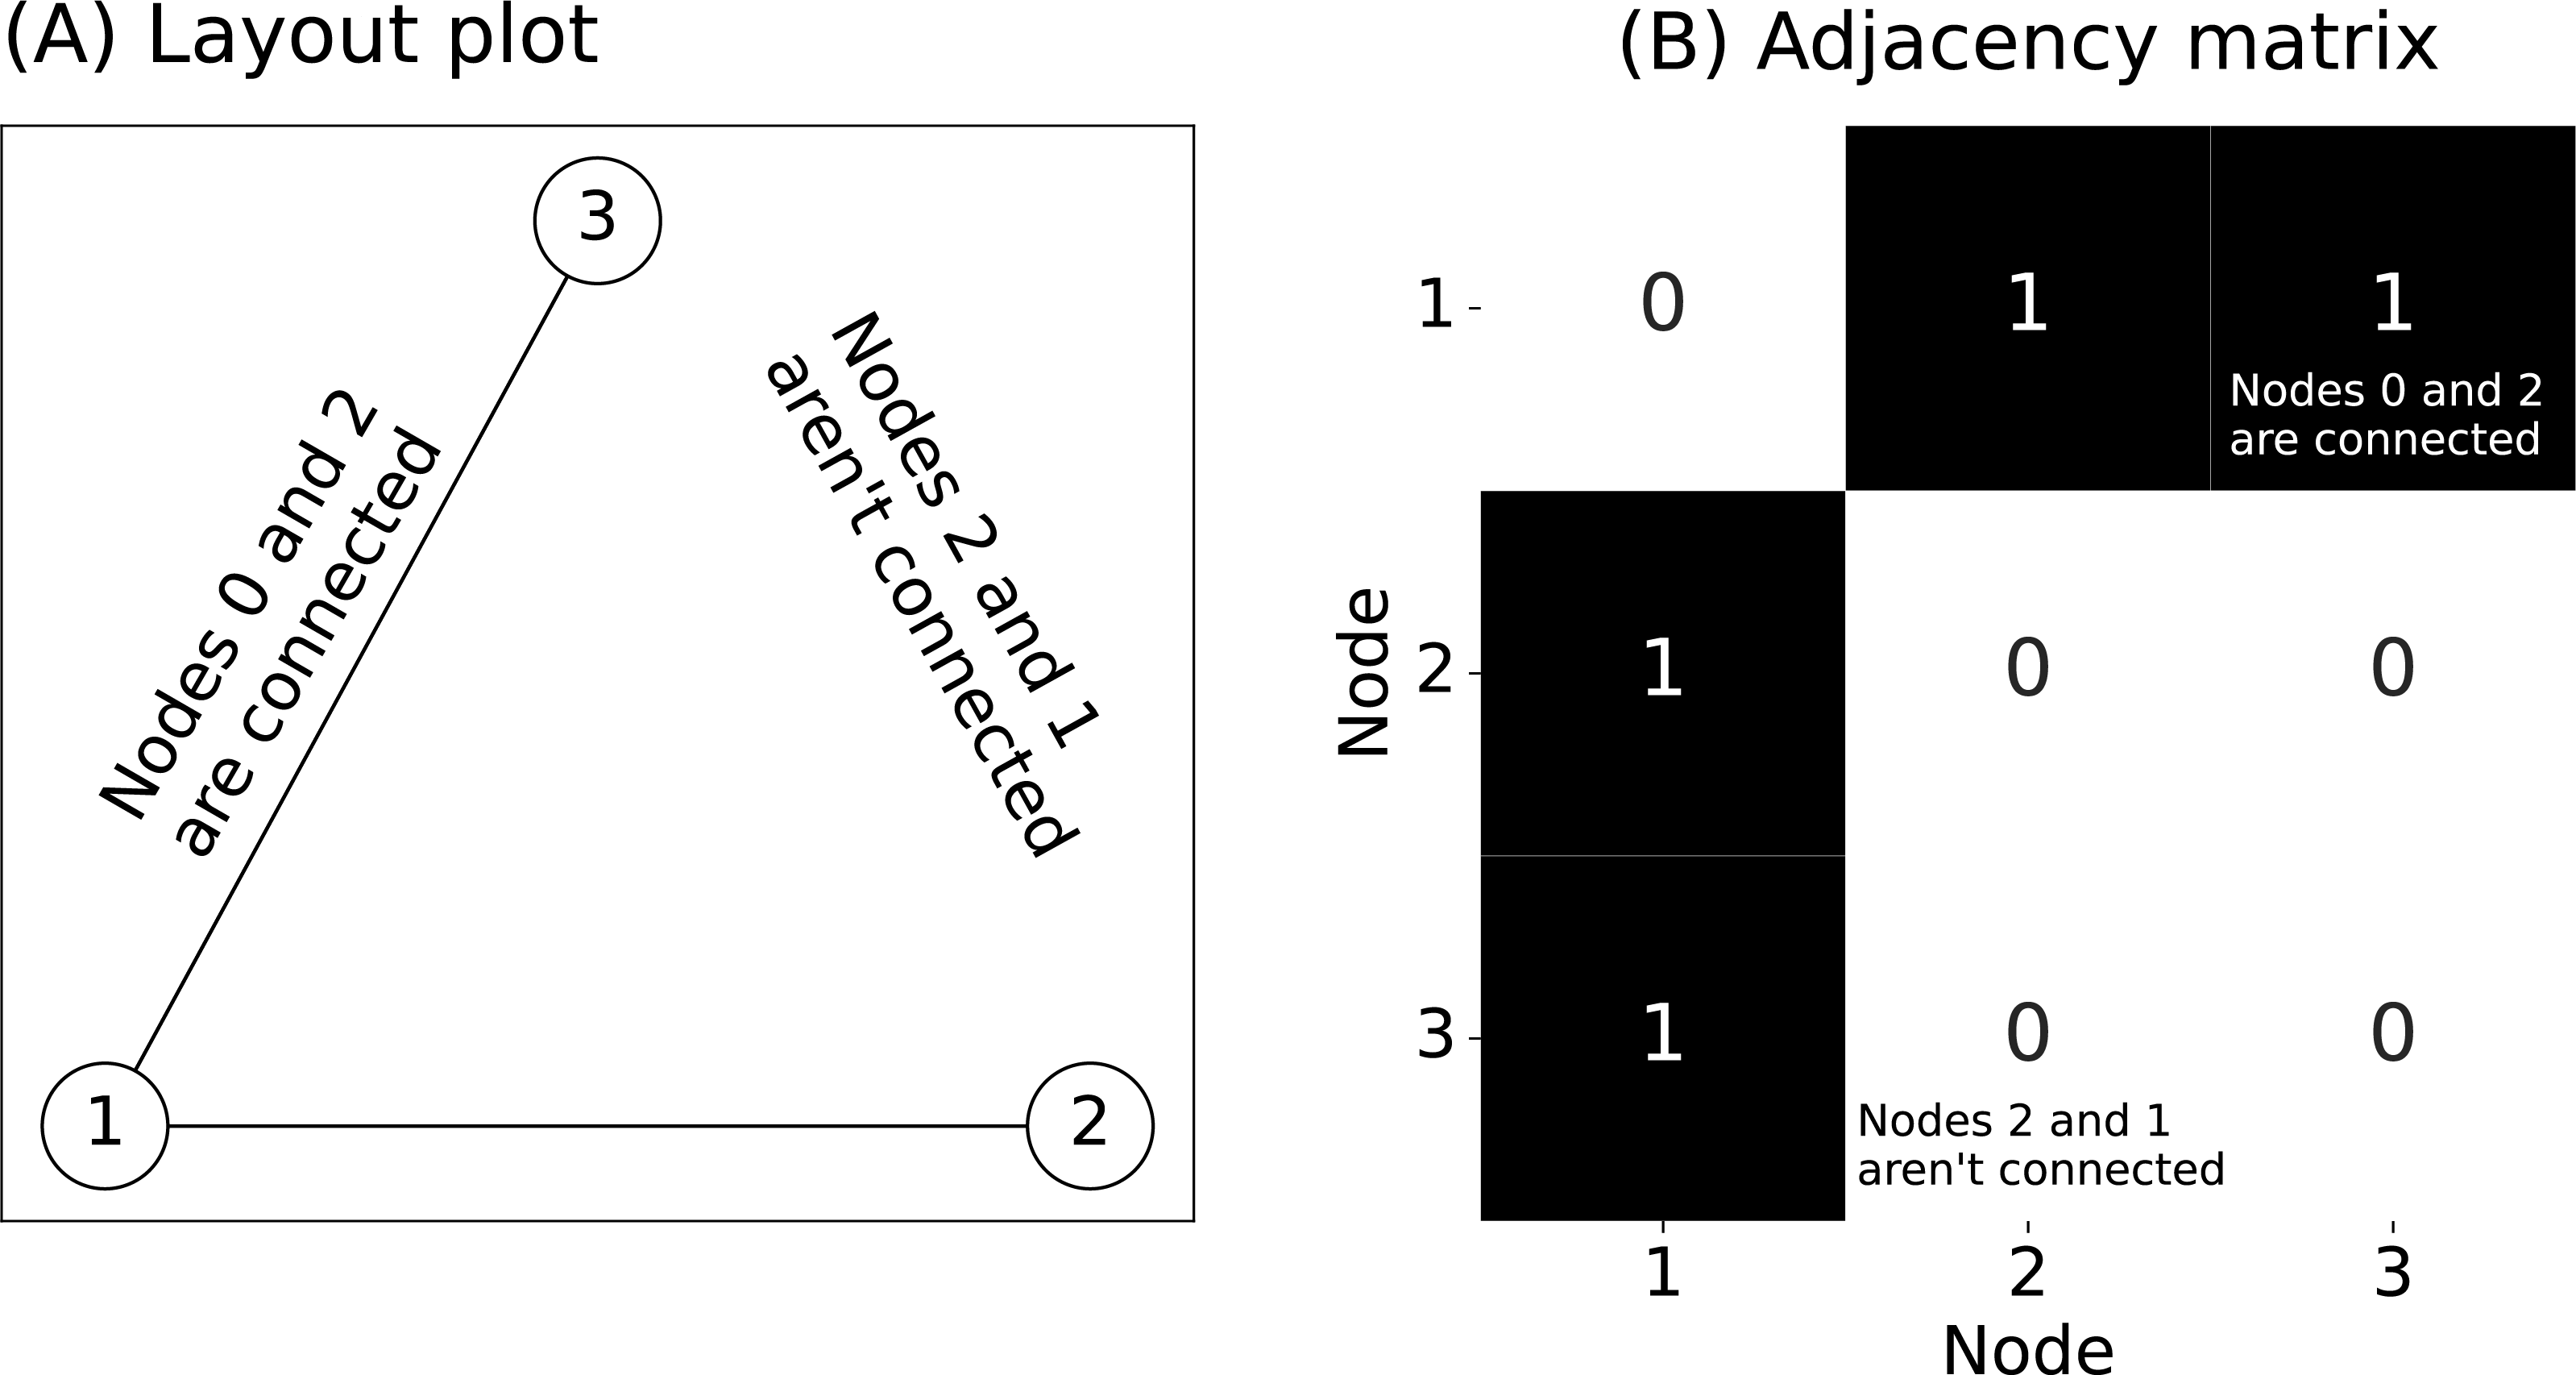
\includegraphics[width=0.8\linewidth]{representations/ch4/Images/basic_mtxs.png}
    \caption[Plotting a simple network as a layout plot and adjacency matrix heatmap]{\textbf{(A)} A layout plot of the network, where nodes are circles and edges are the lines connecting them. \textbf{(B)} the network, visualized as an adjacency matrix.}
    \label{fig:ch4:basic_mtxs}
\end{figure}

\subsection{The degree matrix}

The degree matrix isn't a full representation of our network, because we wouldn't be able to reconstruct an entire network from a degree matrix. However, it's fairly straightforward and it pops up relatively often as a step in creating other matrices, so the degree matrix is useful to mention. It's just a diagonal matrix with the values along the diagonal corresponding to the number of each edges each node has, also known as the \textit{degree} of each node. We'll learn more about the degree matrix in Section \ref{sec:ch4:prop-net}.

We can see the degree matrix for our network below. The diagonal element corresponding to node $1$ has the value of two, since it has two edges; the rest of the nodes have a value of $1$, since they each are only connected to the first node.

\begin{lstlisting}[style=python]
# Build the degree matrix D
degrees = np.count_nonzero(A, axis=0)
D = np.diag(degrees)
# plot it

heatmap(D, annot=True, linewidths=.1, cbar=False, 
        title="Degree matrix $D$", 
        xticklabels=[1,2,3], yticklabels=[1,2,3]
       ).set(xlabel="node", ylabel="node");

\end{lstlisting}
The degree matrix is shown in Figure \ref{fig:ch4:simple_lap}.

\subsection{The Laplacian Matrix}

The standard, cookie-cutter Laplacian Matrix $L$ \cite{Chung1996Dec} is just the adjacency matrix $A$ subtracted from the the degree matrix $D$:

\begin{align*}
 L = D - A
\end{align*}

Since the only nonzero values of the degree matrix is along its diagonals, and because the diagonals of an adjacency matrix never contain zeroes if its network doesn't have nodes connected to themselves, the diagonals of the Laplacian are just the degree of each node. The values on the non-diagonals work similarly to the adjacency matrix: they contain a $-1$ if there is an edge between the two nodes, and a $0$ if there is no edge.

The code below shows us what the Laplacian looks like. Since each node has exactly two edges, the degree matrix is just a diagonal matrix of all twos. The Laplacian looks like the degree matrix, but with -1's in all the locations where an edge exists between nodes $i$ and $j$. We can compute it using:

\begin{lstlisting}[style=python]
L = D - A
\end{lstlisting}

A plot of the Laplacian matrix as a heatmap, along with the degree and adjacency matrices, is shown in Figure \ref{fig:ch4:simple_lap}.
\begin{figure}[h]
    \centering
    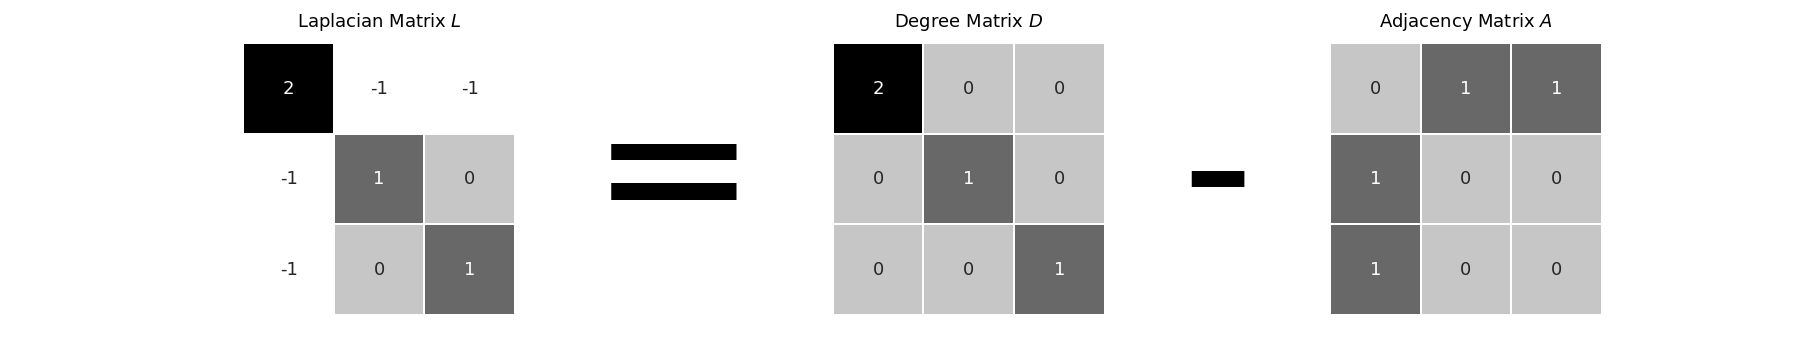
\includegraphics[width=\linewidth]{representations/ch4/Images/simple_lapl.png}
    \caption[Laplacian matrix]{The Laplacian matrix, along with the components that are used to compute it (the degree matrix and the adjacency matrix).}
    \label{fig:ch4:simple_lap}
\end{figure}

We use the Laplacian in practice because it has a number of interesting mathematical properties which tend to be useful for analysis. For instance, the magnitude of its second-smallest eigenvalue, called the Fiedler eigenvalue, tells us how well-connected our network is -- the number of eigenvalues equal to zero is the number of connected components our network has (a concept you will be introduced to in Section \ref{sec:ch4:prop-net:lcc}). Incidentally, this means that the smallest eigenvalue of the Laplacian will always be 0, since any simple network always has at least one ``island''. We don't need to have too much intuition for what eigenvalues mean, but just be aware that they will matter somewhat later on for now.

Another interesting property of the Laplacian is that the sum of its diagonals is twice the number of edges in the network. Because the sum of the diagonal matrix is the trace, and the trace is also equal to the sum of the eigenvalues, this means that the sum of the eigenvalues of the Laplacian is equal to twice the number of edges in the network.

Laplacians and adjacency matrices will be used throughout this book, and details about when and where one or the other will be used are in Chapter \ref{sec:ch6}.

\subsection{The Normalized Laplacian}
\label{sec:ch4:mat-rep:normlapl}

There are a few variations on the standard $D-A$ version of the Laplacian which are widely used in practice, and which (confusingly) are often also called the Laplacian. They tend to have similar properties. The Normalized Laplacian, $L^{norm.}$ is one such variation. The Normalized Laplacian \cite{Chung1996Dec} is defined as:

\begin{align*}
    L^{norm.} = D^{-1/2} L D^{-1/2} = I - D^{-1/2} A D^{-1/2}
\end{align*}

Where $I$ is the identity matrix (the square matrix with all zeroes except for ones along the diagonal). You can work through the algebra yourself if you'd like to verify that the second expression is the same as the third.

Below we can see the normalized Laplacian in code. We use \texttt{graspologic}'s \texttt{to\_laplacian()} function, with the \texttt{form} set to \texttt{I - DAD}, which computes $L^{norm.}$ above.
 
\begin{lstlisting}[style=python]
from graspologic.utils import to_laplacian
L_sym = to_laplacian(A, form="I-DAD")
\end{lstlisting}
A heatmap of the normalized Laplacian is shown in Figure \ref{fig:ch4:normlapl}(A).

We can understand the normalized Laplacian from the name: we can think of it as the Laplacian normalized by the degrees of the nodes associated with a given entry.

We can see this by looking at what the operation is doing:

\begin{align*}
    L^{norm.} &= D^{-\frac{1}{2}}L D^{-\frac{1}{2}} \\
    &= \begin{bmatrix}
        d_{1} & & \\
        & \ddots & \\
        & & d_n
    \end{bmatrix}^{-\frac{1}{2}}\begin{bmatrix}
        l_{11} & ... & l_{1n} \\
        \vdots & \ddots & \vdots \\
        l_{n1} & ... & l_{nn}
    \end{bmatrix}
    \begin{bmatrix}
        d_{1} & & \\
        & \ddots & \\
        & & d_n
    \end{bmatrix}^{-\frac{1}{2}} \\
    &= 
    \begin{bmatrix}
        \frac{1}{\sqrt{d_1}} & & \\
        & \ddots & \\
        & & \frac{1}{\sqrt{d_n}}
    \end{bmatrix}\begin{bmatrix}
        l_{11} & ... & l_{1n} \\
        \vdots & \ddots & \vdots \\
        l_{n1} & ... & l_{nn}
    \end{bmatrix}
    \begin{bmatrix}
        \frac{1}{\sqrt{d_1}} & & \\
        & \ddots & \\
        & & \frac{1}{\sqrt{d_n}}
    \end{bmatrix} \\
    &= \begin{bmatrix}
        \frac{l_{11}}{d_1} & ... & \frac{l_{1n}}{\sqrt{d_1}\sqrt{d_n}} \\
        \vdots & \ddots & \vdots \\
        \frac{l_{n1}}{\sqrt{d_n}\sqrt{d_1}} & ... & \frac{l_{nn}}{d_n}
    \end{bmatrix}
\end{align*}
So the normalized laplacian has entries $l^{norm.}_{ij} = \frac{l_{ij}}{\sqrt{d_i}\sqrt{d_j}}$.

We can plug in the value of $L$ to obtain a similar relationship with the adjacency matrix $A$. Notice that:
\begin{align*}
    L^{norm.} &=  D^{-\frac{1}{2}}L D^{-\frac{1}{2}} \\
    &=  D^{-\frac{1}{2}}(D - A) D^{-\frac{1}{2}} \\
    &= D^{-\frac{1}{2}}DD^{-\frac{1}{2}} - D^{-\frac{1}{2}}A D^{-\frac{1}{2}} \\
    &= D^{\frac{1}{2}}D^{-\frac{1}{2}} - D^{-\frac{1}{2}}A D^{-\frac{1}{2}} \\
    &= I_{n \times n} - D^{-\frac{1}{2}}A D^{-\frac{1}{2}}
\end{align*}

The $D^{-1/2} D D^{-1/2}$ term is spiritually the same as what we'd think of $\frac{D}{D}$ (if that was defined!), since it just works out to be the identity matrix. The $D^{-1/2} A D^{-1/2}$ is just doing the same thing to $A$ that we did to $L$. So we're normalizing the entries of the adjacency matrix by the degrees of the nodes a given entry is concerned with; that is, $\frac{a_{ij}}{\sqrt{d_i}\sqrt{d_j}}$.

One useful property of the normalized Laplacian is that its eigenvalues are bounded between 0 and 2. This normalization tends to be useful, because the Laplacian is a thing called a \emph{positive semi-definite matrix}. This means that a suite of linear algebra techniques, which may \emph{not} run successfully on the adjacency matrix (which is \emph{not} positive semi-definite in its most raw form for \emph{simple networks}, which we will learn about in the next chapter), can be executed on the network Laplacian. For more details about the properties of the Laplacian, check out \cite{Li2014Dec}.

\subsection{The \texttt{DAD} Laplacian}
\label{sec:ch4:mtx-rep:dad_laplacian}

In this book, a lot of what we will cover will be something called a \emph{spectral embedding} of the Laplacian. While we will learn all about this in Section \ref{sec:ch6:lse}, there are some fine points we want to cover here. As it turns out, there is another, \emph{related}, definition of a Laplacian, which we call the \texttt{DAD} Laplacian:

\begin{align*}
    L^{DAD} &= D^{-\frac{1}{2}}A D^{-\frac{1}{2}}
\end{align*}

$L^{DAD}$ and $L^{norm.}$ share some major similarities which are important to note here. Later in the book in Section \ref{sec:ch6:lse}, you will learn about the importance of the singular value decomposition for spectral embedding of Laplacians. Basically, what the singular value decomposition will allow us to do is look at the laplacian as a sum of much \emph{simpler} matrices. By ``simple'', what we mean here is that they can be represented as the product of two vectors. By looking only at the first few of these ``simple'' matrices, we can learn about the Laplacian and reduce a lot of noise in the Laplacian itself. The properties of looking at the \texttt{DAD} Laplacian are discussed at length in \cite{Chaudhuri2012Jun} and \cite{Amini2012Jul},

The most important connection is that these "simple" matrices will be \emph{identical} for $L^{norm.}$ and $L^{DAD}$, except for one important fact: they will be in \emph{reverse} order from one another. In $L^{norm}$, the matrices we will want to use will be the last few, and in $L^{DAD}$, the matrices we will want to use will be the first few. When we compute the singular value decomposition, there are ways to only compute the first few matrices without having to go through the trouble of computing \emph{all} of them, whereas the reverse is not true! To get the last few simple matrices, we would have to compute all of the preceding ones first. This means that to get the simple matrices we want, we can get much better computational performance using $L^{DAD}$ instead of $L^{norm}$.

We can compute the $L^{DAD}$ in \texttt{graspologic} similarly to above, but with \texttt{form="DAD"}:

\begin{lstlisting}[style=python]
L_dad = to_laplacian(A, form="DAD")
\end{lstlisting}

A heatmap of the \texttt{DAD} Laplacian is shown in Figure \ref{fig:ch4:normlapl}(B).

\subsection{The regularized Laplacian}
\label{ch4:mtx-rep:reg_laplacian}
The regularized Laplacian is an adaptation of the \texttt{DAD} Laplacian we learned about in the previous section. As it turns out, when networks have degree matrices where some of the degrees are really, really small, the \emph{spectral clustering} approach we will learn about in Section \ref{sec:ch7:comm_detect} is simply not going to perform very well. When we say it is not going to perform very well, what we mean is that the spectral clusterings are going to be extremely influenced by these nodes with really small node degrees. To overcome this hurdle, instead of using the \texttt{DAD} Laplacian, we can use the regularized Laplacian, defined extremely similarly to the \texttt{DAD} Laplacian, as:

\begin{align*}
    L^{rDAD}(\tau) &= D_\tau^{-\frac{1}{2}}A D_\tau^{-\frac{1}{2}}
\end{align*}

Where $\tau$ is a regularization constant which is greater than or equal to zero, and $D_\tau = D + \tau I$. When we put $\tau$ in parentheses here (that is, $(\tau)$), all that we mean is that $L^{rDAD}$ is a function of the particular regularization constant that we choose. Basically, what this is going to do is just "inflate" the diagonal elements of the degree matrix. So, if the degree for some of the nodes is extremely small, when we add a constant $\tau$ to them, we can increase the degrees by $\tau$. In effect, what this will do is make the nodes with really small degrees (which, like we said, might cause issues in the spectral clustering) a lot less impactful on the results that we obtain. Also, as we can see, if $\tau = 0$, then $L^{rDAD}(\tau) = L^{DAD}$. The regularized Laplacian is discussed at length in \cite{Qin2013Sep}.

Let's take a look at what $L^{rDAD}(\tau)$ and $L^{DAD}$ look like when we pick $\tau$ to be $1$. We can do this in \texttt{graspologic} using \texttt{form="R-DAD"}, and then setting \texttt{regularizer} appropriately:
\begin{lstlisting}[style=python]
tau = 1
L_rdad = to_laplacian(A, form="R-DAD", regularizer=tau)
\end{lstlisting}
The \texttt{R-DAD} Laplacian is shown in Figure \ref{fig:ch4:normlapl}(C).

We will learn about some other ways to handle nodes with very low degrees in Section \ref{sec:ch4:regularization} on Regularization.

\begin{figure}[h]
    \centering
    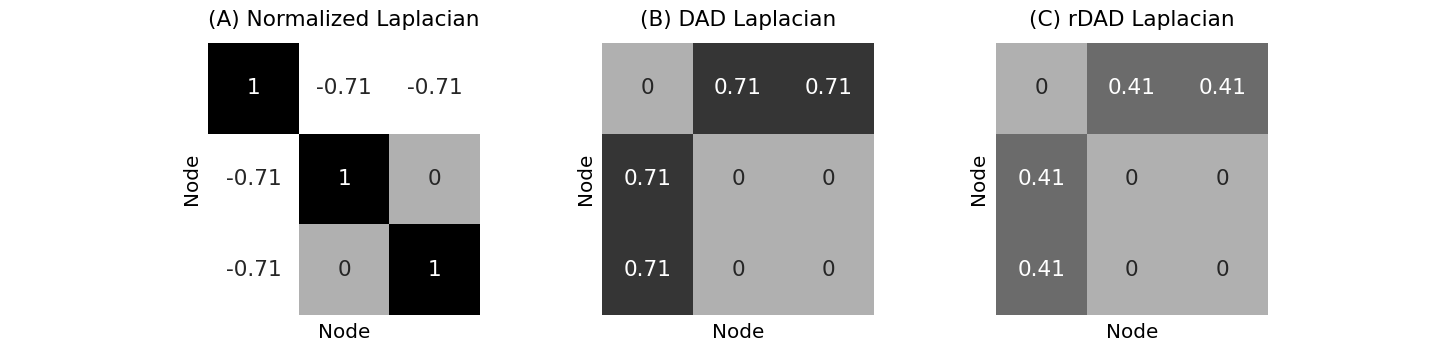
\includegraphics[width=\linewidth]{representations/ch4/Images/normlapls.png}
    \caption[comparison of normalized Laplacians]{Different variations of Laplacians for the same underlying network.}
    \label{fig:ch4:normlapl}
\end{figure}

\newpage
\section{Properties of networks}
\label{sec:ch4:prop-net}


\subsection{Descriptive Properties of Networks}

Remember that with a network, we can represent the collection of nodes and edges as an $n \times n$ adjacency matrix, where $n$ is the total number of nodes. The adjacency matrix looks like this:

\begin{align*}
    A &= \begin{bmatrix}
        a_{11} & ... & a_{1n} \\
        \vdots & \ddots & \vdots \\
        a_{n1} & ... & a_{nn}
    \end{bmatrix},
\end{align*}

Let's say you have a network representing the five boroughs of New York (Staten Island SI, Brooklyn BK, Queens Q, the Bronx BX, and Manhattan MH). The nodes in your network are the five boroughs. The edges $(i,j)$ of your network exist if one can travel from borough $i$ to borough $j$ along a bridge. Let's start by defining a network for ourselves with \texttt{networkx}'s \texttt{DiGraph()} function:


\begin{lstlisting}[style=python]
import networkx as nx
from graphbook_code import heatmap

# create an undirected network G
G = nx.Graph()
# add the nodes like before
G.add_node("SI", pos=(2,1))
G.add_node("MH", pos=(4,4))
G.add_node("BK", pos=(4,1.7))
G.add_node("Q", pos=(6,3))
G.add_node("BX", pos=(6,6))

# specify boroughs that are connected to one another
pos = nx.get_node_attributes(G, 'pos')
G.add_edge("SI", "BK")
G.add_edge("MH", "BK")
G.add_edge("MH", "Q")
G.add_edge("MH", "BX")
G.add_edge("Q", "BX")

A = nx.to_numpy_array(G)

# plotting
nx.draw_networkx(G, with_labels=True, node_color="black", pos=pos,
                font_color="white", edge_color="black")

# pass in the xticklabels and yticklabels corresponding to the
# appropriately ordered boroughs (in the order we constructed them)
heatmap(A.astype(int), xticklabels=["SI", "MH", "BK", "Q", "BX"],
            yticklabels=["SI", "MH", "BK", "Q", "BX"], 
       ).set(xlabel="Borough", ylabel="Borough")
\end{lstlisting}

Figure \ref{fig:ch4:nyc_ex} shows a plot of the bridges of New York, a layout plot representation of a network derived from the the boroughs of New York, and an adjacency matrix as a heatmap of this network.

In this section, we're going to discuss a number of descriptive measures and summary statistics about networks. For a detailed overview, there are a lot of great references out there; some of our favorites are \cite{Barabsi2013Mar}, \cite{Gross2005Sep}, and \cite{Newman2006Jun}, to name a few.

\begin{figure}
    \centering
    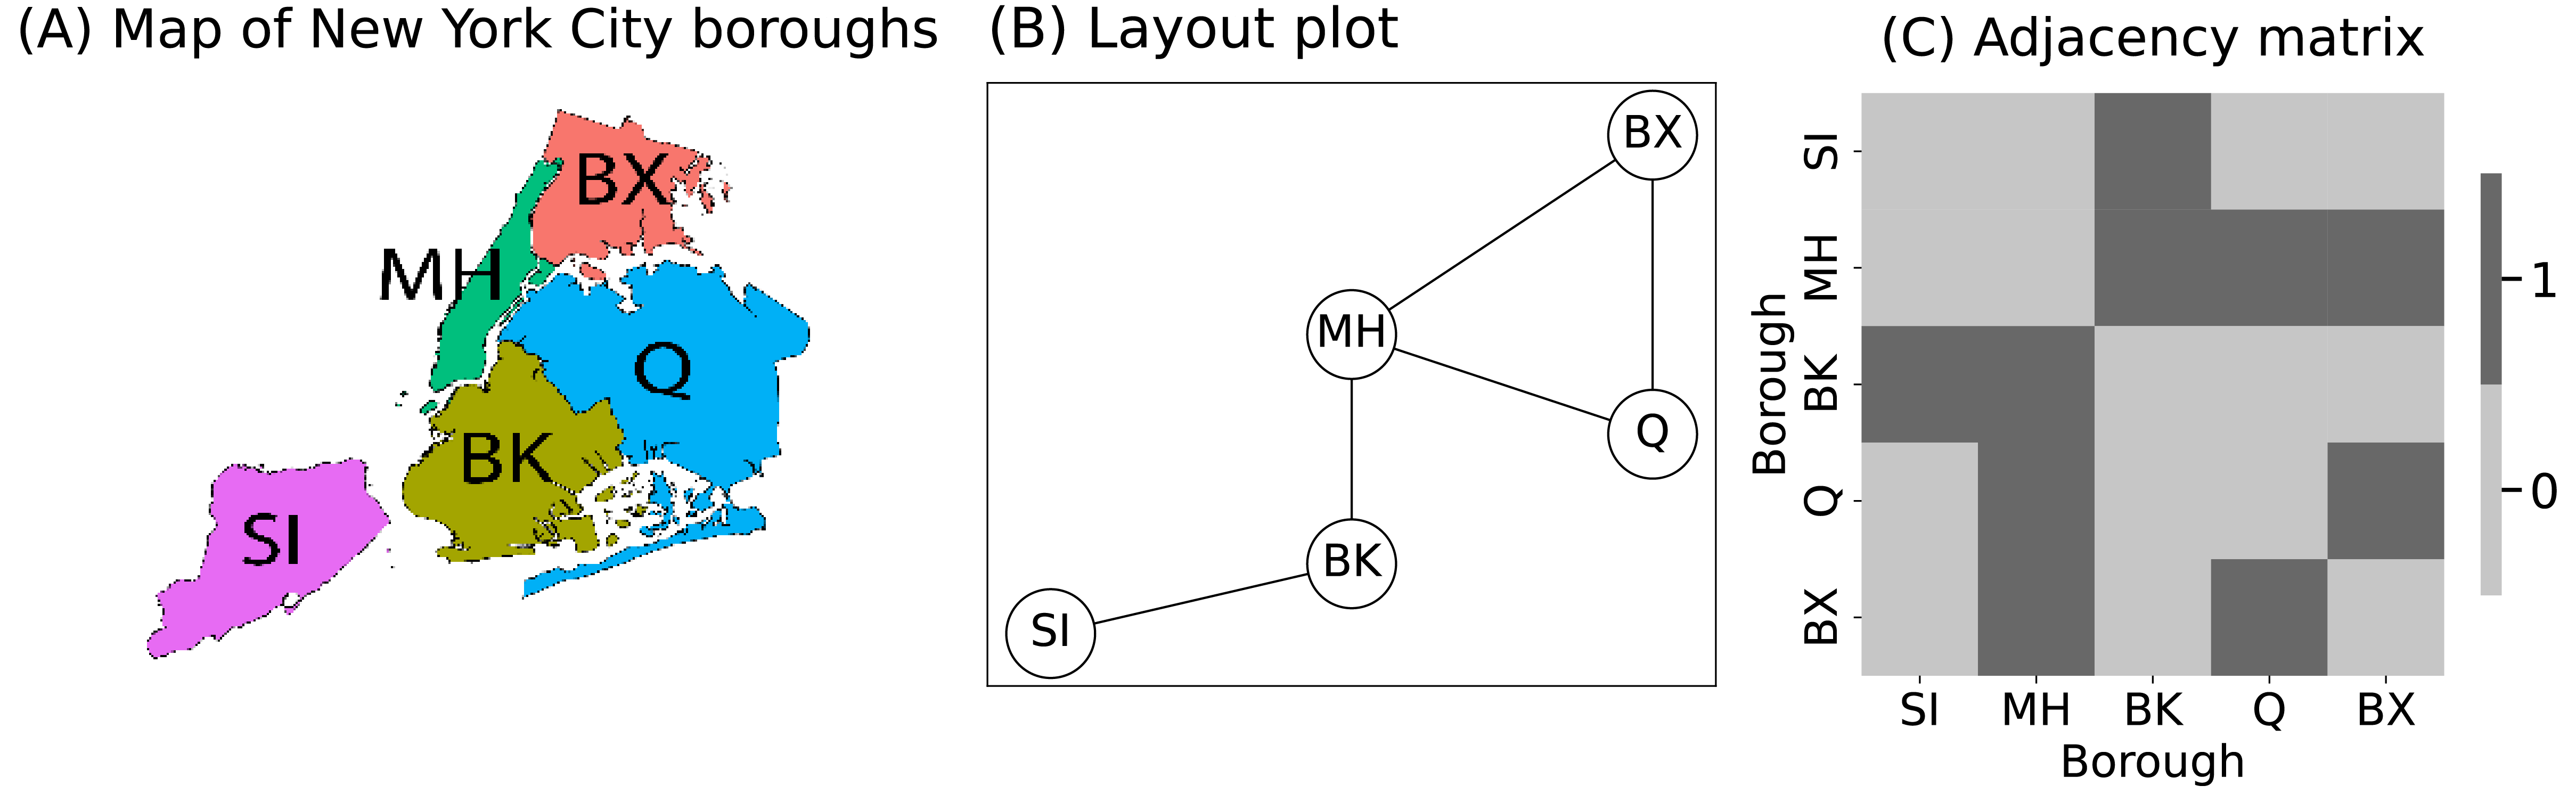
\includegraphics[width=\linewidth]{representations/ch4/Images/nyc_ex.png}
    \caption[New York City borough example]{\textbf{(A)} a map of New York, with the bridges that connect different boroughs. We use this to construct a network of New York, where the nodes are boroughs of New York and the edges are bridges between different boroughs. \textbf{(B)} the network visualized as a layout plot. \textbf{(C)} the network visualized as a heatmap.}
    \label{fig:ch4:nyc_ex}
\end{figure}

\subsection{The edges of undirected networks are bi-directional}

When you decide to travel from borough $i$ to borough $j$, you care about whether you can {actually drive} in that direction. In a similar way, the concept of directedness describes whether you need to worry about one-way bridges and bridge closures. If your network contains one-way bridges, then a bridge from borough $i$ to borough $j$ doesn't {necessarily} imply that a bridge from borough $j$ to borough $i$ exists (just ask New York drivers). If, for instance, the Brooklyn bridge was closed from Brooklyn to Manhattan, your network might change like this. Note that there is no arrow going from Brooklyn to Manhattan, so you cannot drive directly from MH to BK. We can do this by removing the edge from MH to BK:

\begin{lstlisting}[style=python]
from copy import deepcopy

G_dir = G.to_directed()
# remove the edge from MH to BK
G_dir.remove_edge("BK", "MH")

nx.draw_networkx(G_dir, with_labels=True, node_color="black", pos=pos,
                font_color="white", arrows=True, edge_color="black")
\end{lstlisting}

Basically, the arrows of the directed network tell you which nodes you can travel between. Note that we passed the \texttt{arrows="True"} argument, which tells \texttt{networkx} to include the arrows in our plot. A plot of this network is shown in Figure \ref{fig:ch4:directed}(B). Note that there are bi-directional arrows (arrows from one node to the other, as well as the reverse) for all pairs of nodes except Brooklyn and Manhattan.

\begin{figure}[h]
    \centering
    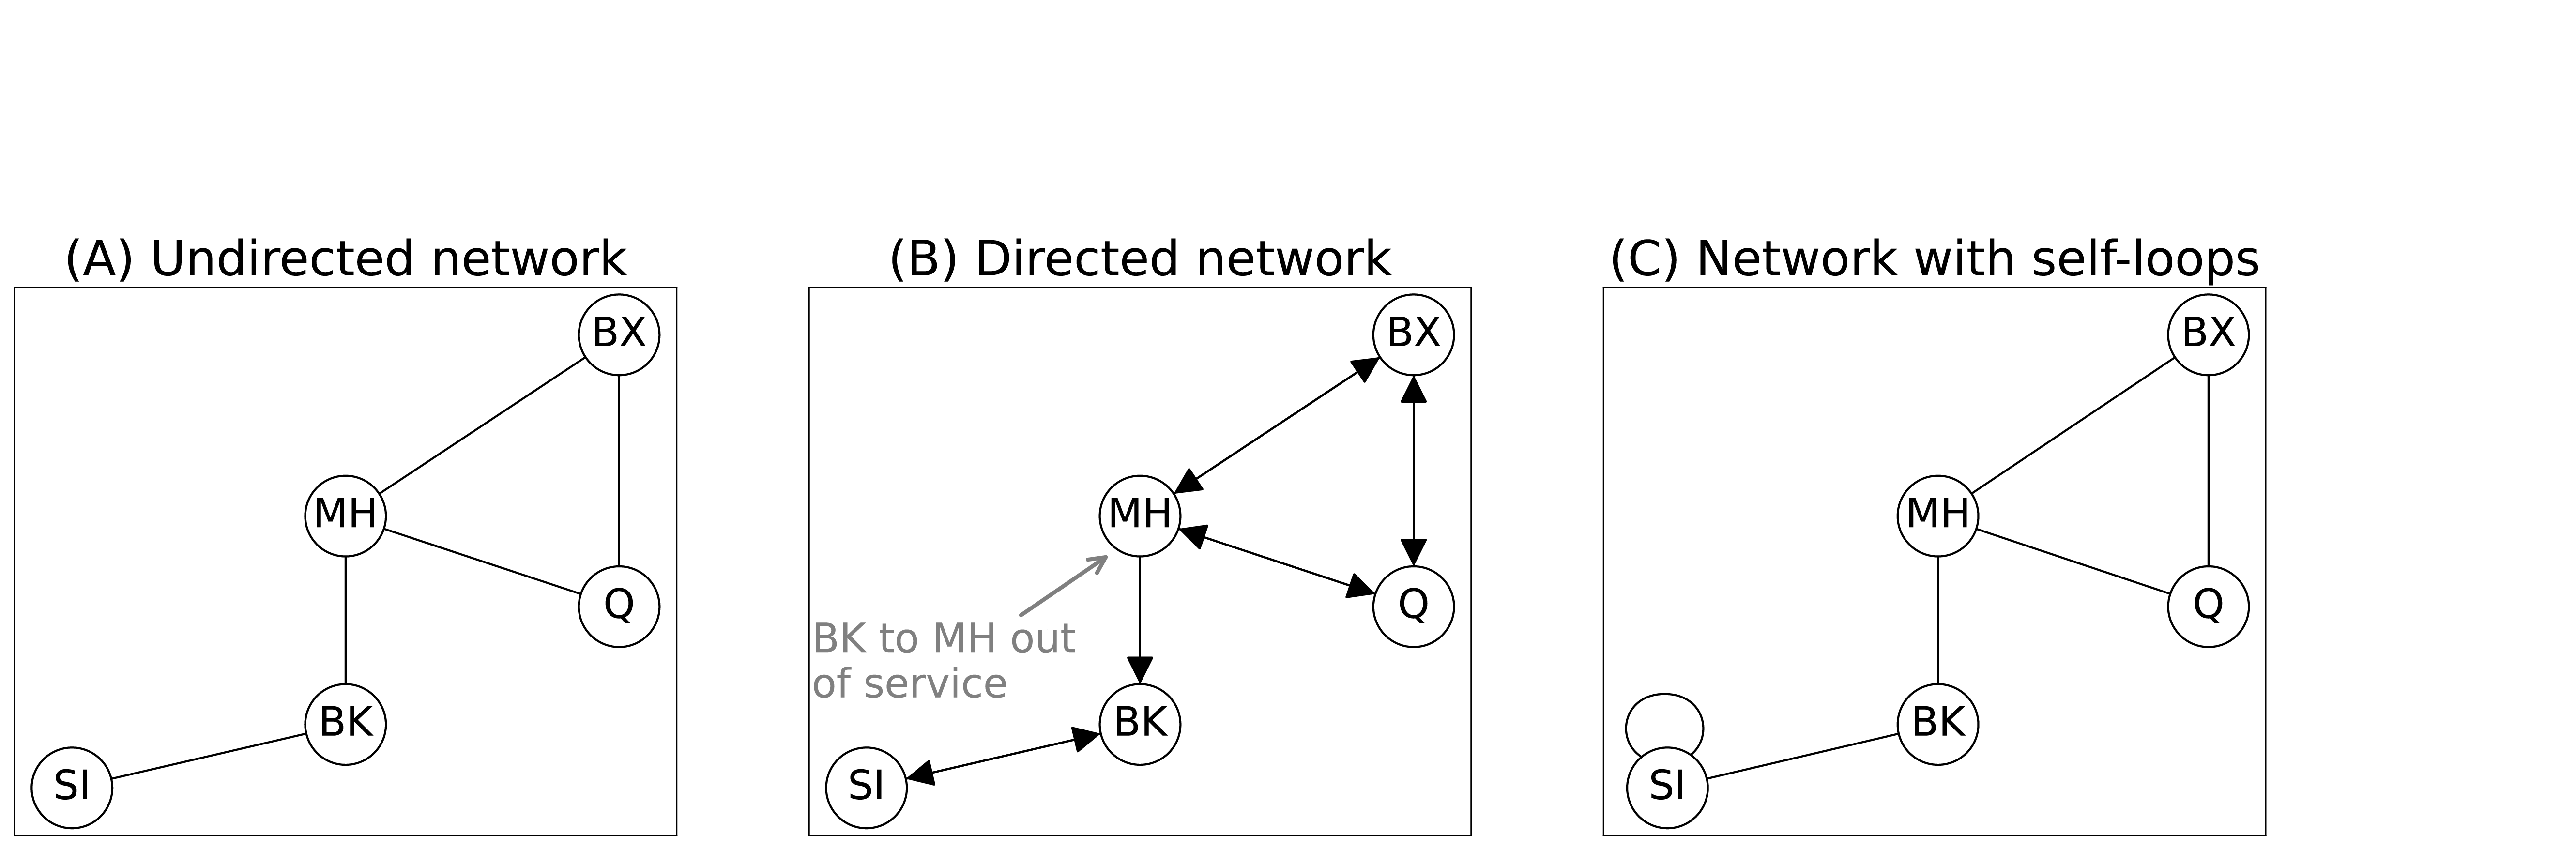
\includegraphics[width=\linewidth]{representations/ch4/Images/directed.png}
    \caption[Comparing directed and undirected networks]{\textbf{(A)} The undirected network. \textbf{(B)} A plot of the network with the bridge from BK to MH out of service. \textbf{(C)} a plot of the network with a self-loop.}
    \label{fig:ch4:directed}
\end{figure}

In the context of this book, we will usually only worry about the undirected case, or when the presence of an arrow implies that the other direction exists, too. A network is \textit{undirected} if an edge between node $i$ and node $j$ implies that node $j$ is also connected to node $i$. 

A plot of the undirected network is shown in Figure \ref{fig:ch4:directed}(A). For the adjacency matrix $A$, remember an edge between nodes $i$ and $j$ is represented by the adjacency $a_{ij}$. This means that if the network is undirected, $a_{ij} = a_{ji}$, for all pairs of nodes $i$ and $j$. By definition, this tells us that the adjacency matrix $A$ is \textit{symmetric}, so $A = A^\top$. We can verify this condition with \texttt{graspologic}:
\begin{lstlisting}[style=python]
from graspologic.utils import is_symmetric

A = nx.to_numpy_array(G)
is_symmetric(A)
# True
A_dir = nx.to_numpy_array(G_dir)
is_symmetric(A_dir)
# False
\end{lstlisting}

\subsubsection{Loopless networks do not have self-loops}

If you are already in a borough, why would you want to take a bridge to that same borough? This logic relates to the concept of {self-loops} in a network. A \textit{self-loop} in a network describes whether nodes can connect back to themselves. For instance, consider the following loop on Staten Island. This would have the interpretation of a bridge which connects Staten Island back to itself:
\begin{lstlisting}[style=python]
G_loopy = deepcopy(G)
# add edge from SI to itself
G_loopy.add_edge("SI", "SI")
nx.draw_networkx(G_loopy, with_labels=True, node_color="black", pos=pos,
                font_color="white", edge_color="black")
\end{lstlisting}

A plot of this network is shown in Figure \ref{fig:ch4:directed}(C). A network is \textit{loopless} if self-loops are not possible. It is also important to note that both directed and undirected network can have self-loops; we only show the undirected case.

For the adjacency matrix $A$, a self-loop would be represented by the adjacencies $a_{ii}$ for all nodes $i$. Note that these entries $a_{ii}$ are all of the {diagonal} entries of $A$. Therefore, for a network which is loopless, all adjacencies $a_{ii}$ on the diagonal {do not exist}. Mathematically, we will represent this by saying that the diagonal entries are $0$, which means that the matrix is \textit{hollow}. You might also see this property abbreviated by stating that the diagonal of the adjacency matrix is $0$, or $diag(A) = 0$. It is important to understand that if the network is loopless, there is a theoretical distinction between $0$ and {does not exist}. Denoting the diagonal in an adjacency matrix of a loopless network with $0$ is a convenience and a convention for the field. This distinction will make a difference in later sections of this chapter, so be ready!

We can verify this condition using: 

\begin{lstlisting}[style=python]
from graspologic.utils import is_loopless
is_loopless(A)
# True
A_loopy = nx.to_numpy_array(G_loopy)
is_loopless(A_loopy)
# False
\end{lstlisting}


\subsubsection{Unweighted networks either have an edge, or they don't}

Do you need to convey information about how long it takes to get from borough $i$ to borough $j$ with your network? The broader fundamental question here -- whether an edge needs to carry extra information besides its existence -- underlies the concept of {weightedness} in networks. In a weighted network, you could use {edge-weights} $w(i, j)$ to describe the amount of time it takes to get from borough $i$ to borough $j$. An \textit{edge-weight} $w(i,j)$ assigns a weight to an edge between nodes $i$ and $j$ if that edge exists. If you care about weightedness in the network, the network is called {weighted}. 

The potential edges $a_{ij}$ of $A$ for a weighted network take the value of the edge-weight; that is, $a_{ij} = w(i, j)$ for any edge which exists between nodes $i$ and $j$. In the below plot, edge-weight indicates the approximate time to travel from one borough to the other. The network is undirected, so you don't have to worry about directionality differences. The edge-weight is indicated by the number along the corresponding edge.

\begin{lstlisting}[style=python]
G_weight = nx.Graph()

G_weight.add_node("SI", pos=(2,1))
G_weight.add_node("MH", pos=(4,4))
G_weight.add_node("BK", pos=(4,1.7))
G_weight.add_node("Q", pos=(6,3))
G_weight.add_node("BX", pos=(6,6))

# this time, we add weights to the edges
pos = nx.get_node_attributes(G, 'pos')
G_weight.add_edge("SI", "BK", weight=20)
G_weight.add_edge("MH", "BK", weight=15)
G_weight.add_edge("MH", "Q", weight=15)
G_weight.add_edge("MH", "BX", weight=5)
G_weight.add_edge("Q", "BX", weight=15)

A_weight = nx.to_numpy_array(G_weight)

nx.draw_networkx(G_weight, with_labels=True, node_color="black", pos=pos,
                 font_color="white", edge_color="black")

heatmap(A_weight, xticklabels=["SI", "MH", "BK", "Q", "BX"],
        yticklabels=["SI", "MH", "BK", "Q", "BX"], title="Weighted adjacency matrix", 
        font_scale=1.3, xtitle="Borough", ytitle="Borough")
\end{lstlisting}
We can identify whether a network is unweighted using \texttt{is\_unweighted()}:


\begin{lstlisting}[style=python]
from graspologic.utils import is_unweighted

A_weight = nx.to_numpy_array(G_weight)
is_unweighted(A)
# True
is_unweighted(A_weight)
# False
\end{lstlisting}
In a lot of your data analyses, you will come across weighted networks, so we give you an example of what they will look like in Figure \ref{fig:ch4:weighted}.

For most examples in this book, you will usually discuss {unweighted} or {binary} networks. A network is \textit{unweighted} or \textit{binary} if you only care about whether edges are {present} or {absent}. In an unweighted network, a potential edge $a_{ij}$ takes the value $1$ if there is an edge from node $i$ to node $j$, and takes the value $0$ if there is {not} an edge from node $i$ to node $j$.

\begin{figure}
    \centering
    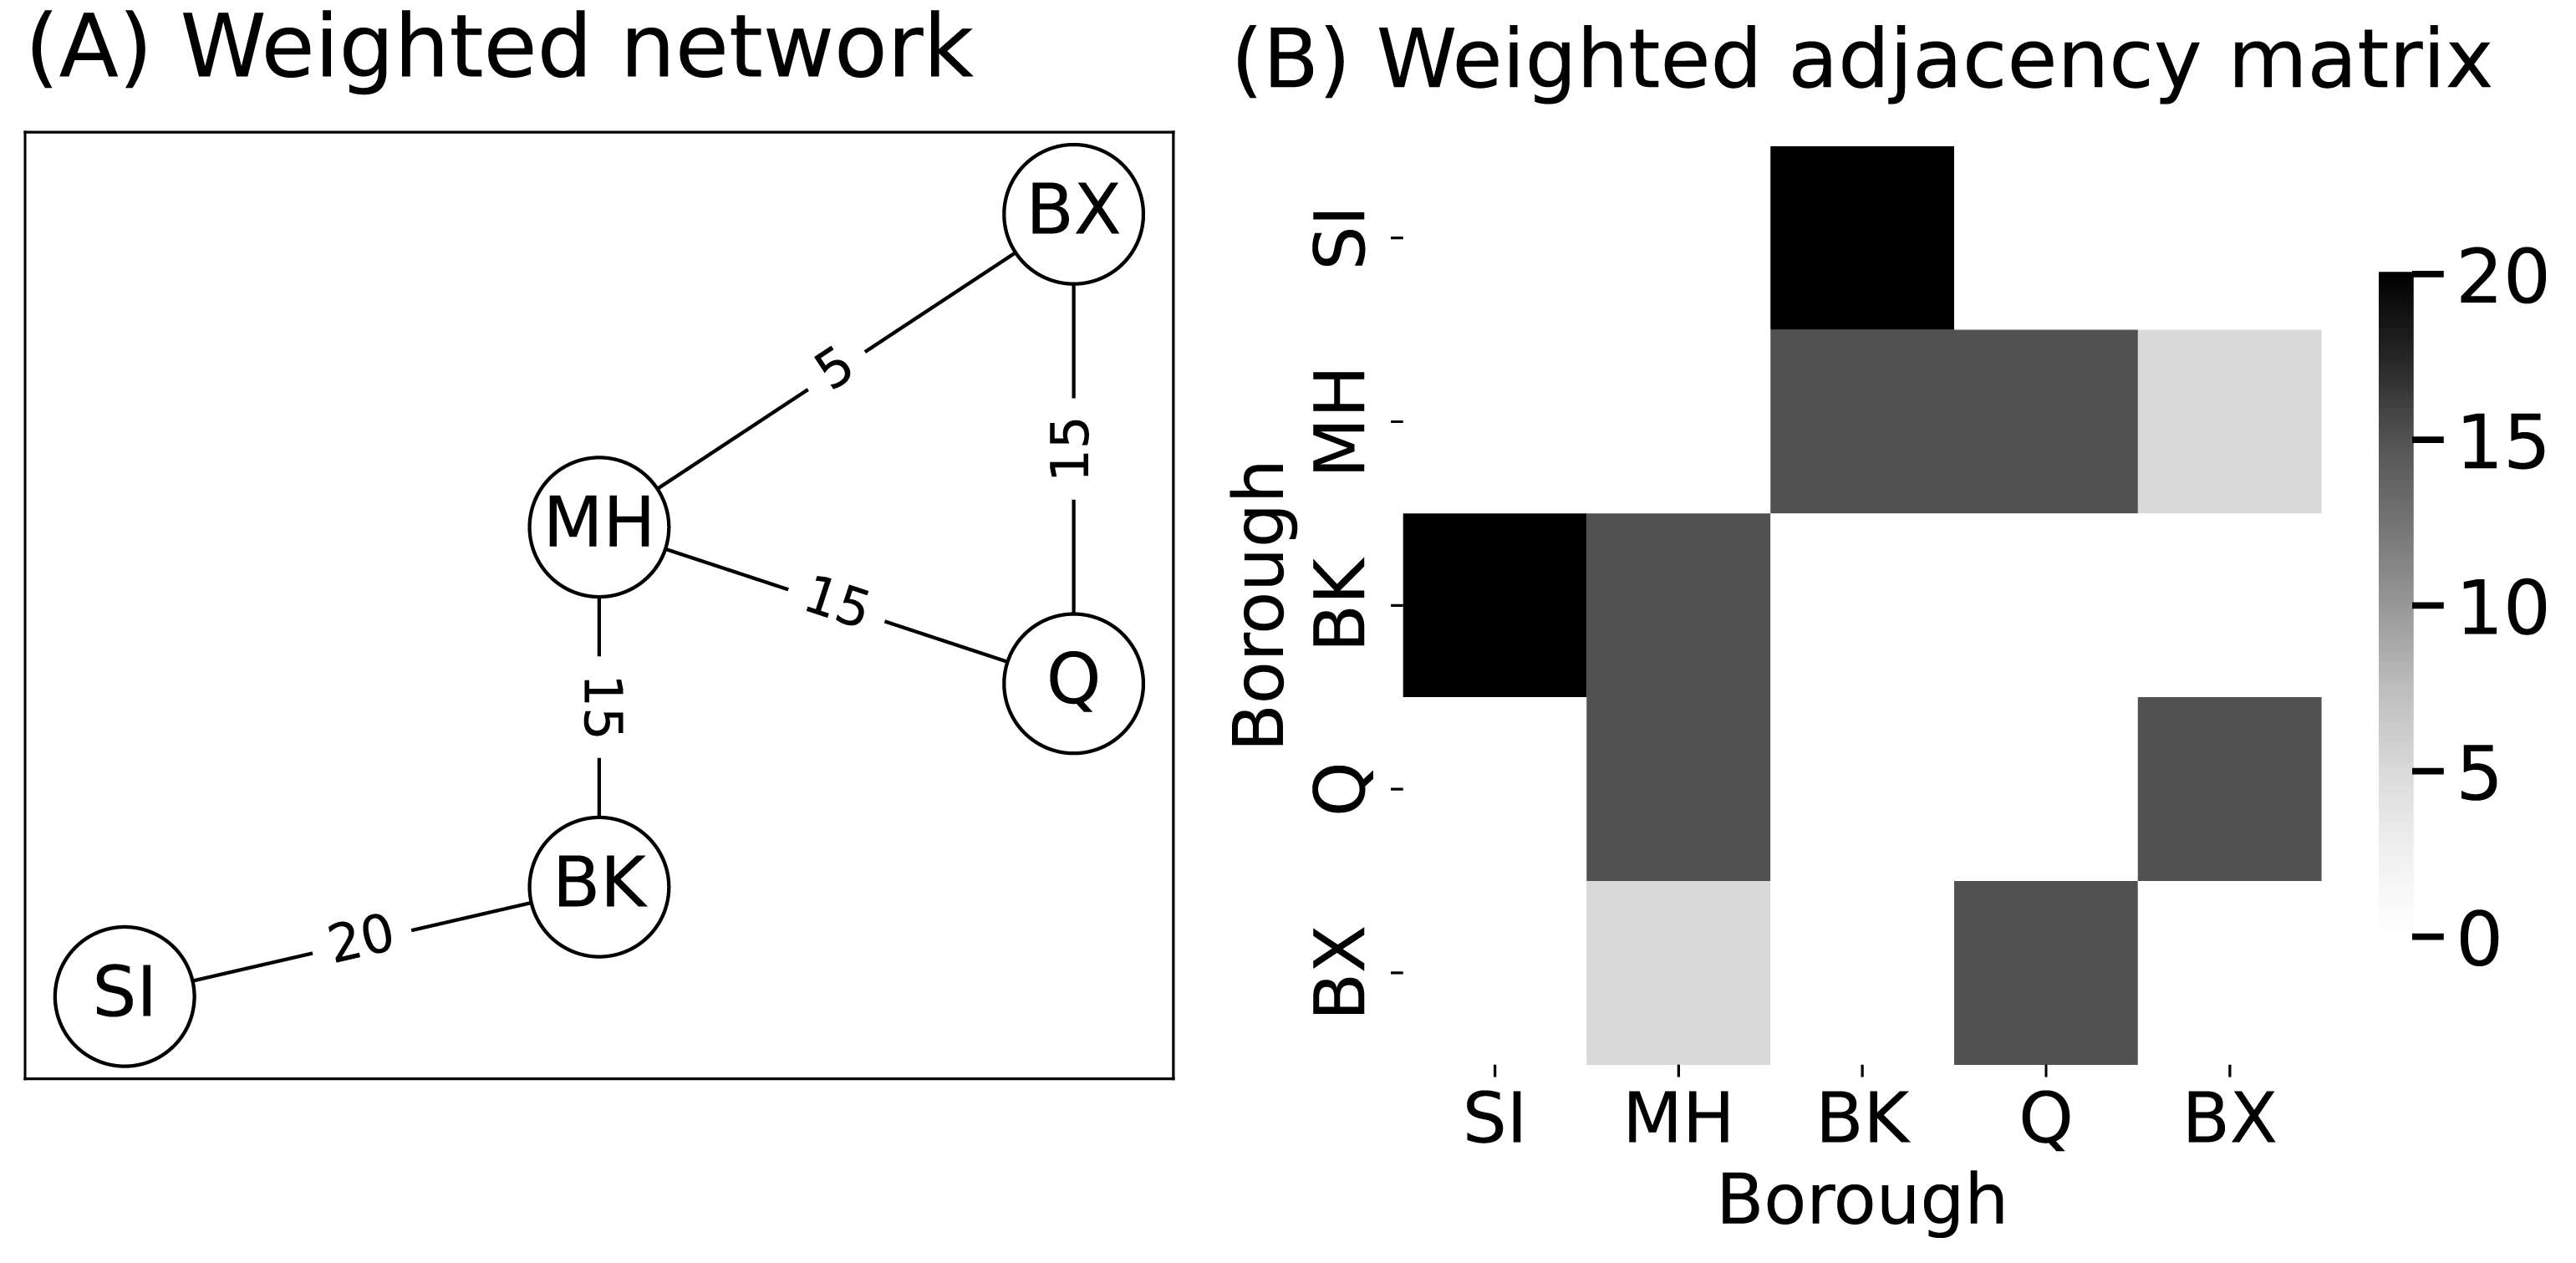
\includegraphics[width=0.8\linewidth]{representations/ch4/Images/weighted.png}
    \caption[Weighted network in New York borough example]{The New York City borough network, where weights indicate the travel times across the indicated bridges. \textbf{(A)} a layout plot for the weighted network, and \textbf{(B)} a heatmap of an adjacency matrix for the weighted network.}
    \label{fig:ch4:weighted}
\end{figure}

\begin{floatingbox}[h]\caption{This book considers {simple networks}}
A \textit{simple network} is loopless, undirected, and unweighted. Most of the examples and techniques you look at in this book are developed in the context of simple networks. Fortunately, this note is largely conceptual, and doesn't really impact much from an implementation perspective. All the techniques and packages you use will make sensible choices, or will directly extend, to cases that fall outside of this particular setup. If your networks don't satisfy one or any of these properties, most of the approaches discussed herein will still work. 

If the technique will not work for the network you have provided, the software package used (such as \texttt{networkx}, \texttt{graspologic}, or \texttt{igraph}) will probably either give you a warning or an explicit error if there is a substantial issue with the network you have provided. That said, when implementing network analysis methods on your own, we strongly encourage you to double check with the documentation to ensure that it is {compatible} with the type of network you are analyzing.
\end{floatingbox}

\subsection{Descriptive Properties of Nodes}

Just like you have many words and properties which describe the network itself, you also have special vocabulary in network machine learning to describe properties about the individual nodes in the network. We'll learn some of the ones here that will come up again later in the book.

\subsubsection{Node neighbors and incidences}

You begin by describing properties of single nodes in a simple network. The simplest property of a network is {adjacency}. A pair of nodes $i$ and $j$ in an undirected network are \textit{neighbors} if an edge exists between them. In terms of the adjacency matrix, two nodes $i$ and $j$ are neighbors if the potential edge $a_{ij}$ is one.

\subsubsection{Node degree quantifies the number of edges}
\label{sec:ch4:prop-net:degree}
The simplest summary statistic for a node is known as the {node degree}. The \textit{node degree} of $i$ in a simple network is the number of nodes with which it is a neighbor. Remember that if two nodes are not neighbors, the adjacency matrix entry corresponding to this {potential} edge takes a value of zero. This means that we can just count the potential edges $a_{ij}$ for a node $i$ to get its degree. We do this by just summing the $i^{th}$ row (or equivalently, if the network is simple, its $i^{th}$ column):

\begin{align}
    d_i &= degree(i) \triangleq \sum_{j = 1}^n a_{ij} = \sum_{j = 1}^n a_{ji}\label{eqn:ch4:degree}
\end{align}

Now you might be thinking, this isn't just counting edges which exist, since it counts {every} potential edge for node $i$. Let's see how that holds up. Remember that if an edge exists, $a_{ij}$ takes a value of $1$, whereas if an edge does not exist, $a_{ij}$ takes a value of $0$. This means that every $a_{ij}$ is either zero or one, so you can write:

\begin{align*}
    d_i &= \sum_{j = 1}^n a_{ij} \\
    &= \sum_{j : a_{ij} = 1} a_{ij} + \sum_{j : a_{ij} = 0}a_{ij} \\
    &= \sum_{j : a_{ij} = 1}1 + 0
\end{align*}
Note that in the left sum, since every $a_{ij}$ is defined to be one, that this is just the number of times that $a_{ij}$ takes a value of one, which is all of the edges that node $i$ touches. The right sum has every $a_{ij}$ defined to be zero, so this is just zero!

For instance, if you consider the node BK in your example, BK touches two edges, indicated in bold in  Figure \ref{fig:ch4:degree}(A), so $degree({BK}) = 2$. When you look at the corresponding adjacency matrix, if you sum the entries for node ${BK}$, you also get two. The entries which would be summed row-wise or column wise for ${BK}$ are shown in black boxes, in Figure \ref{fig:ch4:degree}(B).

\begin{figure}[h]
    \centering
    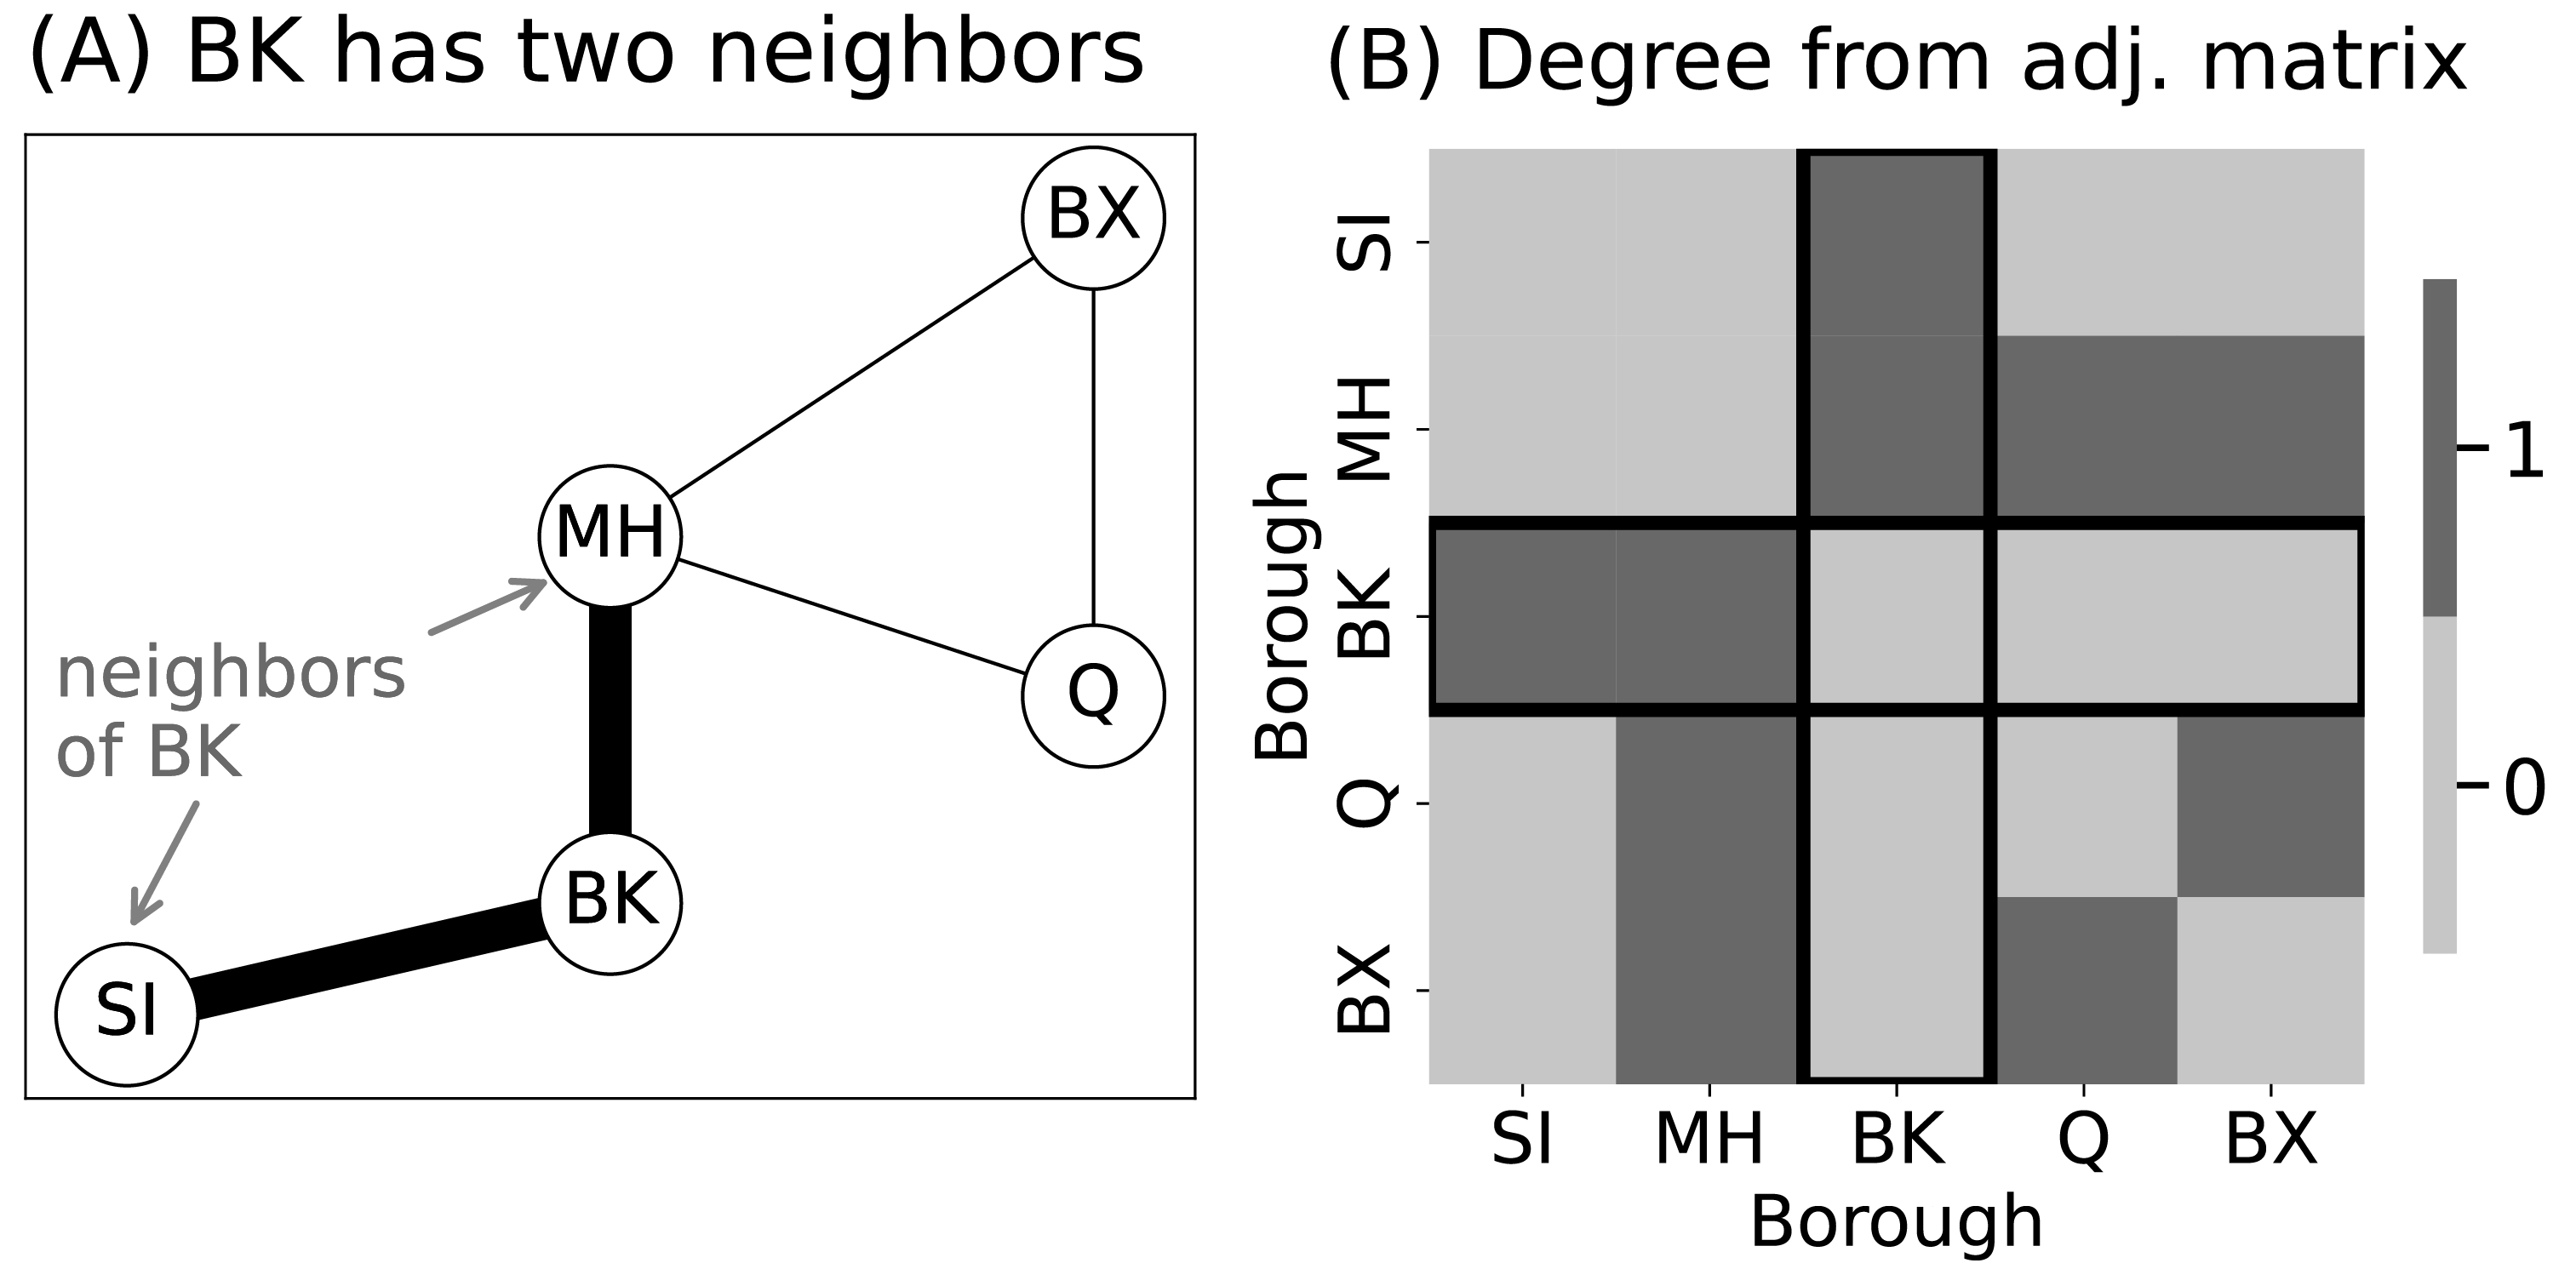
\includegraphics[width=0.8\linewidth]{representations/ch4/Images/degree.png}
    \caption[Deriving node degree from layout and adjacency matrix heatmaps]{A case-study of the BK borough. \textbf{(A)} shows that BK has two neighbors, SI and MH (edges to SI/MH are bold-faced). \textbf{(B)} shows the axes of the adjacency matrix could be summed to derive this fact as well. Note the row/column corresponding to BK (black boxes) has a sum value of two.}
    \label{fig:ch4:degree}
\end{figure}

It really doesn't matter whether you sum row or column-wise, as long as you pick one, if the network is undirected.

\subsubsection{The degree matrix indicates the degrees of each node}

A useful quantity which you will come across in many of the later chapters of this book is called the {degree matrix} of the network. The degree matrix is the {diagonal} matrix:
\begin{align*}
    D &= \begin{bmatrix}
        d_1 & 0 & ... & 0 \\
        0 & \ddots & \ddots& \vdots \\
        \vdots & \ddots & \ddots & 0 \\
        0 & ... & 0 & d_n
    \end{bmatrix}, \;\;\; d_i = degree(i)
\end{align*}
This matrix $D$ is called \textit{diagonal} because all of the entries $d_{ij} = 0$ unless $i = j$. The diagonal entries $d_{ii}$ of the degree matrix are simply the node degrees $degree(i)$ for each node $i$. Using the counting procedure you described above, you can see that the node SI has degree one, the node BK has degree two, the node MH has degree three, the node Q has degree two, and the node BX has degree two. We can compute the degree matrix for an unweighted network by using either of the following commands:

\begin{lstlisting}[style=python]
# summing column-wise
D_column = np.diag(A.sum(axis=0))
# summing row-wise
D_row = np.diag(A.sum(axis=1))
\end{lstlisting}

You can plot the degree matrix using the \texttt{heatmap} utility that we developed for the adjacency matrix.

\paragraph{Degrees for directed networks}

A question you might have in the back of your head is, "what if the network is directed?" When the network is directed, you have two types of degrees, the {in degree} and the {out degree}. The \textit{in degree} of a node $i$ in a directed network is the number of nodes which have edges that go {to} node $i$. Remember that the column of the adjacency matrix, $a_{ji}$, where $j$ indexes all of the nodes of the network, take a value of $1$ if node $j$ has a directed edge from itself to node $i$. This means that to compute the in-degree for node $i$, we just need to sum its column of the adjacency matrix:
\begin{align*}
    d_i^{in} &= \sum_{j = 1}^n a_{ji}
\end{align*}
On the other hand, the \textit{out degree} of a node $i$ is the number of nodes that node $i$ has edges which point to. By the exact same logic, the row of the adjacency matrix $a_{ij}$, where $j$ indexes all of the nodes of the network, takes a value of $1$ if node $i$ has a directed edge from itself to some other node $j$. This means that to compute the out-degree for node $i$, we just need to sum its row of the adjacency matrix:
\begin{align*}
    d_i^{out} &= \sum_{j = 1}^n a_{ij}
\end{align*}
In an undirected network, since $a_{ji} = a_{ij}$ these quantities are equal, which is how we ended up with the nice relationship in the preceding section. 

In a directed network, since there is no concept of a {node degree} like there was for an undirected network, we instead have two degree matrices: the {in-degree matrix} $D^{in}$ and the {out-degree matrix} $D^{out}$. The \textit{in-degree matrix} $D^{in}$ is the matrix whose diagonal entries are the in-degrees of each node $i$ in the network. The \textit{out-degree matrix} $D^{out}$ is the matrix whose diagonal entries are the out-degrees of each node $i$ in the network. 

These can be computed like this:

\begin{lstlisting}[style=python]
# summing column-wise to get out degree
D_out = np.diag(A_dir.sum(axis=0))
# summing row-wise to get in-degree
D_in = np.diag(A_dir.sum(axis=1))
\end{lstlisting}
% @AL: np.sum() is already heavily accelerated, much more so than any matrix multiplication routine, as it is specifically designed for a matrix multiplication with the 1-vector. see the code in numpy.

\paragraph{Degrees for weighted networks}

If the network is weighted, either weighted and directed or weighted and undirected, all of the logic we've learned so far applies directly. Remember that the adjacency matrix $A$ has entries $a_{ij} = w(i, j)$ if the edge exists between nodes $i$ and $j$ and $0$ otherwise. This means that when we compute the degrees (either the undirected node degree, the in-degree, or the out-degree), we instead sum edge weights when the edge exists, and $0$s otherwise.

\subsection{Network summary statistics tell you useful attributes about networks}

When you learn about networks, it is often valuable to compute properties of the network so that you can get a better understanding of the relationships within it. We will call these properties {network summary statistics}. Although this book will focus more on {learned} representations of networks, summary statistics are a sort of {engineered} representation. Next, we will learn several network summary statistics, and in Section \ref{sec:ch4:net-rep:featurelims}, we will explore the limitations of network summary statistics.


\begin{floatingbox}[h]\caption{Short-hands you will come across in network science}
\label{box:ch4:sums}
When dealing with software packages or technical papers on network data, it is often the case that many authors will favor readability and brevity over writing out things with the most unambiguous notation possible. For this reason, there are a number of short-hands that you are going to want to get familiar with. The most common ones are:
\begin{enumerate}
    \item Double sums $\sum_{i = 1}^n \sum_{j = 1}^n x_{ij}$ will often be abbreviated as $\sum_{i, j = 1}^nx_{ij}$. The reason is that $i$ and $j$ are both summing over the same indexing set $\{1, ..., n\}$, and therefore it is redundant to write it twice.
    \item Likewise, triple sums $\sum_{i = 1}^n \sum_{j = 1}^n \sum_{k = 1}^n x_{ijk}$ will often be abbreviated as $\sum_{i,j,k = 1}^nx_{ijk}$.
    \item You might come across ambiguous sums entirely, such as $\sum_{i,j}x_{ij}$. This would mean to sum over all possible values $i$ and $j$ could take that would make sense when considered with the summand (e.g., the $x_{ij}$ term). For example, if $x_{ij}$ are the entries of an $n \times m$ matrix $X$, this sum would be $\sum_{i = 1}^n \sum_{j = 1}^m x_{ij}$. 
    \item You might come across sums that index inequalities, such as $\sum_{i \neq j}x_{ij}$. This means to consider all possible pairs $(i, j)$ where $i \neq j$. You will come across two of these frequently, for square adjacency matrices $A$:
    \begin{itemize}
        \item $\sum_{i \neq j} a_{ij}$, which means $\sum_{i = 1}^n \sum_{j \neq i}a_{ij}$.
        \item $\sum_{j > i} a_{ij}$, which means $\sum_{i = 1}^n \sum_{j = i + 1}^n a_{ij}$.
    \end{itemize}
\end{enumerate}
\end{floatingbox}


\subsubsection{The network density indicates the fraction of possible edges which exist}
\label{sec:ch4:prop-net:density}
Given the adjacency matrix $A$ of a simple network, what fraction of the possible edges {actually} exist? 

To understand this quantity, first you need to understand how many edges are possible in a network. This is where that ``caveat'' about loopless networks come in in a big way: we need to count in such a way that we don't accidentally assume that self-loops are potential edges; since the self-loops are simply not possible, we need to ignore them. 

You have $n$ total nodes in the network, so $A$ is an $n \times n$ matrix. Therefore, $A$ has $n^2$ total entries. However, it turns out that over {half} of these entries are redundant for simple networks. Since you are assuming the network is simple, the network is by definition loopless. This means that every entry is {by default} $0$ along the diagonal. Since each node $i$ has a corresponding diagonal entry $a_{ii}$, this comes to $n$ entries that you do not need to count. This leaves your total possible number of edges at $n^2$ (the total number of entries in the matrix $A$) minus $n$ (the total number of entries which are automatically $0$), or $n^2 - n = n(n - 1)$. This quantity represents the total number of possible edges which are {not} in the diagonal.

What else are we overcounting? Well, as it turns out, if the network is also {undirected} (which it is, because it is {simple}), every node that is {not} in the diagonal is also being double counted. Why is this? Remember that an undirected network has an adjacency matrix where for every pair of nodes $i$ and $j$, $a_{ij} = a_{ji}$. This means that you overcount the number of possible edges not in the diagonal by a factor of {two}, since each off-diagonal entry $a_{ij}$ has a corresponding entry $a_{ji}$. This leaves the total number of possible edges in the network as $\frac{1}{2}n(n - 1)$, or the total number of possible edges not in the diagonal reduced by a factor of two. This quantity is notated by $\binom n 2$, which is read as ``$n$ {choose} $2$''. You might see this notation arise in the study of {combinatorics}, where it is used to answer the question of, "In how many ways can you {choose} two items from $n$ items?" In the network in Figure \ref{fig:ch4:density}(B), you see all of the {possible} edges indicated. If you count them up, there are $\frac{1}{2}\cdot 5 \cdot (5 - 1) = 10$ possible edges.

Now, how many edges {actually} exist in your network? The sum of all of the entries of $A$ can be represented by the quantity $\sum_{i , j= 1}^n a_{ij}$. For each node $i$, we sum all of the $a_{ij}$, and then we add these across all of the nodes. Remember that $A$ is loopless, so you don't need to count the diagonal entries. This brings your quantity to $\sum_{i \neq j}a_{ij}$, since you don't need to count any edges along the diagonal of $A$. Next, remember that if an edge in $A$ exists between nodes $i$ and $j$, that {both} $a_{ij}$ and $a_{ji}$ take the value of $1$, due to the undirected property. To obtain the edge count of $A$, that you only need to count {either} $a_{ij}$ {or} $a_{ji}$. Somewhat arbitrarily in this book, we will always count the entries $a_{ij}$ in the upper triangle of $A$, which are the entries where $j > i$. This brings your quantity to $\sum_{j > i} a_{ij}$. 

The edges in your network will be indicated in Figure \ref{fig:ch4:density}(A), of which there are $5$ total. 

\begin{figure}[h]
    \centering
    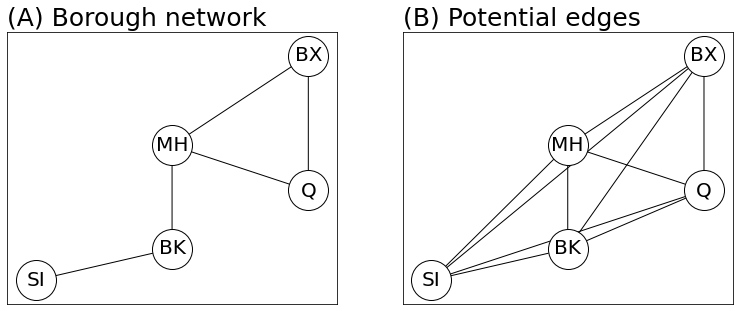
\includegraphics[width=0.8\linewidth]{representations/ch4/Images/density.png}
    \caption[Visualizing network density]{\textbf{(A)} The New York Borough network. The actual edges are shown. \textbf{(B)} The New York Borough network with all possible potential edges.}
    \label{fig:ch4:density}
\end{figure}

To put it all together, the \textit{network density} indicates the {density of edges} which are present in the network. For a simple network, the network density can be defined as the ratio between the total number of edges in $A$ and the total number of edges possible in $A$:
\begin{align}
    density(A) &= \frac{\sum_{j > i}a_{ij}}{\binom n 2} = \frac{2\sum_{j > i}a_{ij}}{n(n - 1)}
    \label{eqn:ch4:netdens}
\end{align}
In your example, this is simply the ratio of edges which {actually} exist to edges which could {possibly} exist, which is $\frac{5}{10} = 0.5$. You can compute the network density via \texttt{networkx} using the function \texttt{density()}:

\begin{lstlisting}[style=python]
nx.density(G)
# 0.5
\end{lstlisting}
In a simple network, there are a few additional ways you might see this equation written. Notice that the following inequality is true, by definition of a simple network:
\begin{align*}
    \sum_{i,j = 1}^n a_{ij} &= \sum_{j > i}a_{ij} + \sum_{i > j}a_{ij} + \sum_{i = 1}^n a_{ii} \\
    &= \sum_{j > i}a_{ij}+ \sum_{i > j}a_{ij} + 0,
\end{align*}
which is because the network is loopless (so the diagonal is $0$). Further, remember that $a_{ij} = a_{ji}$, which means that the first term is {exactly} equal to the second term, so:
\begin{align*}
    \sum_{i,j = 1}^n a_{ij} &= \sum_{j > i}a_{ij}+ \sum_{i > j}a_{ij} \\
    &= \sum_{j > i}a_{ij}+ \sum_{j > i}a_{ij} = 2\sum_{j > i}a_{ij} \\
    \Rightarrow \sum_{j > i}a_{ij} &= \frac{1}{2}\sum_{i,j = 1}^n a_{ij}
\end{align*}
This gives us the useful relationship that we can re-write the density even more simply, by plugging this relationship into Equation \eqref{eqn:ch4:netdens} as:
\begin{align*}
    density(A) &= \frac{\frac{1}{2}\sum_{i = 1}^n \sum_{j = 1}^n a_{ij}}{\binom n 2} = \frac{\sum_{i = 1}^n \sum_{j = 1}^n a_{ij}}{n(n - 1)}
\end{align*}
We wrote out the double sum here because there is a key relationship that we want to point out. Notice that the inner-most sum is just computing the degree $d_i$ of each node $i$, because $d_i = \sum_{j = 1}^n a_{ij}$ in an undirected network. This means that:
\begin{align}
    density(A) &= \frac{\frac{1}{2}\sum_{i = 1}^n d_i}{\binom n 2} = \frac{\sum_{i = 1}^n d_i}{n(n - 1)} \label{eqn:ch4:density_degree}
\end{align}
As a final note, notice that $\frac{1}{n}\sum_{i = 1}^n d_i$ is the \textit{average degree} over all of the $n$ nodes in the network. We will typically abbreviate this quantity using the symbol $d$. Using this fact with the right-most equality in Equation \eqref{eqn:ch4:density_degree}, we see that:
\begin{align*}
    density(A) &= \frac{d}{n - 1}.
\end{align*}
In this sense, the density can be conceptualized as the average degree of each node in the network, divided by the maximum possible degree each node could have (which, in a simple network, is $n-1$, since a node could at most have an edge to the other $n-1$ nodes in the network). This concept will become handy when we think about sparsity in Section \ref{sec:ch10:sparsity}.


\subsubsection{The clustering coefficient indicates how much nodes tend to cluster together}
\label{sec:ch4:prop-net:clustering}

The clustering coefficient indicates the fraction of triplets of nodes which are closed. What the heck is that? Let's look at only Brooklyn, Manhattan, Queens, and the Bronx, and temporarily ignore Staten Island:

\begin{lstlisting}[style=python]
G_clus = nx.Graph()

G_clus.add_node("MH", pos=(4,4))
G_clus.add_node("BK", pos=(4,1.7))
G_clus.add_node("Q", pos=(6,3))
G_clus.add_node("BX", pos=(6,6))


pos = nx.get_node_attributes(G, 'pos')
G_clus.add_edge("MH", "BX")
G_clus.add_edge("MH", "BK")
G_clus.add_edge("MH", "Q")
G_clus.add_edge("Q", "BX")

nx.draw_networkx(G_clus, with_labels=True, node_color="black", pos=pos,
                 font_color="white", edge_color="black")
\end{lstlisting}
The plotted result is shown in \ref{fig:ch4:subnet}(B).

To begin to define the clustering coefficient, you first must understand what a {triplet} is. A \textit{triplet} is an ordered tuple of three nodes which are connected by two or three edges. Note that a tuple of three nodes to be a triplet, you must be able to travel from one end of the triplet to the other along a contiguous path. The triplets are {closed} if there are three edges, and {open} if there are only two edges. For instance, in the above network, you have the following triplets of nodes:
\begin{enumerate}
    \item Open triplets between Bronx, Manhattan, and Brooklyn: (BX, MH, BK), (BK, MH, BX),
    \item Open triplets between Manhattan, Queens, and Brooklyn: (BK, MH, Q), (Q, MH, BK),
    \item Closed triplets between Bronx, Manhattan, and Queens: (BX, MH, Q), (BX, Q, MH), (MH, BX, Q), (MH, Q, BX), (Q, BX, MH), (Q, MH, BX),
\end{enumerate}

To clarify a fine technical point of open triplets, we do not count (BK, Q, MH) as a triplet because there is no edge from BK to Q. You must be able to go from the first node to the second to the third along edges that exist in the network in order for a triple of nodes to count as a triplet. No triplets are possible between Brooklyn, Bronx, and Queens, because only a single edge exists between the three of them. In your example, there are six closed triplets amongst the nodes (delineated in number 3. above), and there are 4 open triplets (delineated in numbers 1. and 2. above). The global clustering coefficient (or transitivity) is defined as:

\begin{align*}
    C &= \frac{\text{number of closed triplets}}{\text{number of closed triplets} + \text{number of open triplets}}
\end{align*}
In our example, this comes to $C = \frac{6}{6 + 4} = 0.6$. This equation can also be understood in terms of the adjacency matrix. Note that if a triplet between nodes $i$, $j$, and $k$ is closed, then all three of the potential edges $a_{ij}$, $a_{jk}$, and $a_{ki}$ have a value of $1$. Therefore, if you could the number of times that $a_{ij}a_{jk}a_{ki} = 1$, you also count the number of closed triplets! This means that the number of closed triplets can be expressed as $\sum_{i,j,k = 1}^na_{ij}a_{jk}a_{ki}$. 

Further, note that for a given node $i$, you can find an arbitrary triplet (either open or closed) through the following procedure.
1. Pick a single neighbor $j$ for node $i$. Note that the node $i$ has a number of neighbors equal to $degree(i) = d_i$, so there are $d_i$ possible neighbors to choose from.
2. Pick a different neighbor $k$ for node $i$. Note that since node $i$ had $d_i$ neighbors, it has $d_i - 1$ neighbors that are not node $j$.
3. Since you know that nodes $j$ and $k$ are both neighbors of node $i$, you know that $a_{ij}$ and $a_{ik}$ both have values of one, and therefore the edges $(i, j)$ and $(i, k)$ exist. Therefore, the tuple of nodes $(i, j, k)$ is a triplet, because {at least} two edges exist amongst the three nodes. This tuple is closed if the edge $(j, k)$ exists, and open if the edge $(j, k)$ does not exist.
4. Therefore, there are $d_i (d_i - 1)$ triplets in which node $i$ is the leading node of the triplet.

As it turns out, since triplets are {ordered tuples}, you can repeat this procedure for all nodes, and if you count how many triplets you get in total, you get the {total number of triplets} for the entire network. Therefore, the number of open and closed triplets in the network is the quantity $\sum_i d_i (d_i - 1)$.  Then you could express the clustering coefficient in terms of the adjacency matrix as:

\begin{align*}
    C &= \frac{\sum_{i,j,k = 1}^n a_{ij}a_{jk}a_{ki}}{\sum_{i = 1}^n d_i (d_i - 1)}
\end{align*}
Which gives you an expression to implement programmatically. You can compute the clustering coefficient via \texttt{networkx} using:

\begin{lstlisting}[style=python]
nx.transitivity(G_clus)
# 0.6
\end{lstlisting}


\subsubsection{The path length describes how far two nodes are}
\label{sec:ch4:prop-net:path}
How many bridges would you need to cross to get from Staten Island to Bronx? This concept relates directly to the concept of the {path length} in a network. A \textit{path} between two nodes $i$ and $j$ is a sequence of edges which starts at node $i$, and traverses through other nodes in the network until reaching node $j$. Two nodes are described as \textit{connected} if a path exists between them. The \textit{path length} is the number of edges in the path. For instance, if you remember your network from the New York example, you could get from Staten Island to Bronx in two possible ways, indicated in in (B) and (C) in Figure \ref{fig:ch4:path}.

\begin{figure}[h]
    \centering
    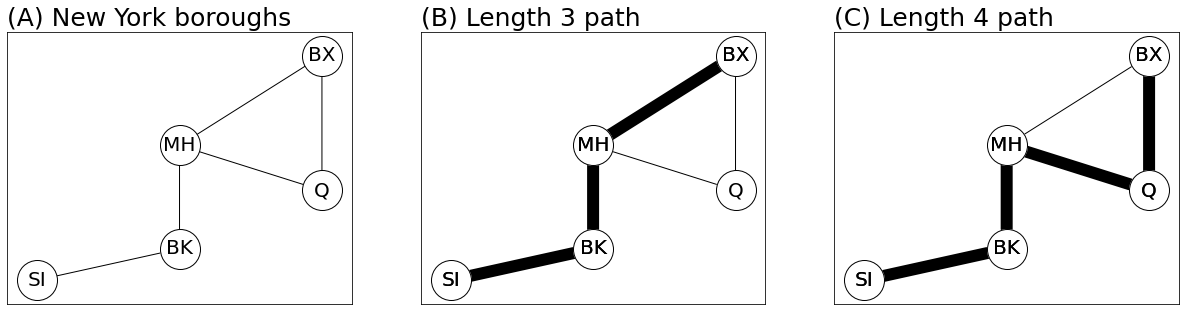
\includegraphics[width=\linewidth]{representations/ch4/Images/path.png}
    \caption[Path length in New York boroughs]{\textbf{(A)} The New York boroughs. \textbf{(B)} A length $3$ path from SI to BX. \textbf{(C)} A length $4$ path from SI to BX.}
    \label{fig:ch4:path}
\end{figure}
In this case, there are only two paths from SI to BX which do not visit the same node more than once, but in a larger network, there may be {many} possible paths from one node to another. For this reason, you will usually be interested in one particular path, the {shortest path}. The \textit{shortest path length} or \textit{distance} between nodes $i$ and $j$ is the path with the smallest path length that connects nodes $i$ and $j$. In your example, the shortest path is indicated by Figure \ref{fig:ch4:path}(B), and the shortest path length is therefore three.  If it is not possible to get from node $i$ to node $j$ using edges of the network, the shortest path length is defined to be infinite. The shortest path between nodes $i$ and $j$ will often be abbreviated using the notation $l_{ij}$.

A common statistic often calculated is the {distance matrix} for the network $L$, which is the $n \times n$ matrix whose entries $l_{ij}$ are the shortest path lengths between all pairs of nodes in the network. For your New York example, you can compute and visualize the distance matrix using:

\begin{lstlisting}[style=python]
L = nx.floyd_warshall_numpy(G)
heatmap(L, title="Distance matrix",  xticklabels=["SI", "MH", "BK", "Q", "BX"],
        yticklabels=["SI", "MH", "BK", "Q", "BX"], xtitle="Borough", ytitle="Borough")
\end{lstlisting}
Another common statistic you can compute using the distance matrix is the {average shortest path length}. The average shortest path length $l$ of a simple network is simply the average of all of the shortest paths between two distinct nodes $i$ and $j$ of the distance matrix:
\begin{align*}
    l &= \frac{1}{n(n - 1)}\sum_{i \neq j} l_{ij}
\end{align*}
The normalizing factor here is $n(n - 1)$ because the sum $\sum_{i \neq j}$ is short-hand for the double-sum $\sum_{i = 1}^n \sum_{j \neq i}$. Notice that the left-most sum has $n$ terms, and for each node $i$, there are $n-1$ other possible values that $j$ can take where $j \neq i$. This means that we are summing $n-1$ terms $n$ times (which is $n (n - 1)$). 

\paragraph{Paths in directed networks}

If the network is directed, the interpretation of a path is exactly the same, except you have to be careful to account for the directionality when finding paths from one node to the next. For instance, in Figure \ref{fig:ch4:directed}(B), there {is} a path from the nodes MH, Q, BX to SI or BK, but there are {no} paths from SI or BK to MH, Q, BX (as the bridge from BK to MH is out of service in the example).

\subsection{Subnetworks are subsets of larger networks}
\label{sec:ch4:prop-net:subnetwork}
When you think of an entire network, it is often useful to consider it in smaller bits. For instance, when you were looking at the clustering coefficient, you found it useful to break out the nodes {BK, Q, BX, MH} so you could count triplets, like we did in Section \ref{sec:ch4:prop-net:clustering}. 

This portion of the network is called a {subnetwork}. A \textit{subnetwork} is a network whose nodes and edges are {subsets} of the nodes and edges for another network. In this case, the  network toplogy of the New York example is $(\mathcal V, \mathcal E)$ defined by the sets:

\begin{enumerate}
    \item The nodes $V$: $\{SI, BK, Q, MH, BX\}$, and
    \item The edges $E$: $\left\{(SI, BK), (BK, MH), (MH, Q), (MH, BX), (Q, BX)\right\}$.
\end{enumerate}

and the subnetwork (which removed Staten Island, SI) we looked at above is the network:

\begin{enumerate}
    \item The nodes $V_s$: $\{BK, Q, MH, BX\}$, and
    \item The edges $E_s$: $\left\{(BK, MH), (MH, Q), (MH, BX), (Q, BX)\right\}$.
\end{enumerate}

As you can see, the subnetwork with nodes and edges $(V_s, E_s)$ is such that every element in $V_s$ is an element of $V$, and therefore the nodes of the subnetwork are a subset of the nodes of the complete network. Further, every element in $E_s$ is an element of $E$, and therefore the edges of the subnetwork are a subset of the edges of the complete network. So the subnetwork $(V_s, E_s)$ is a subnetwork of the network $(V, E)$. This particular subnetwork can be described further as an \textit{induced} subnetwork. A subnetwork of a network is \textit{induced} by a set of nodes if the following conditions hold:

\begin{enumerate}
    \item The nodes $V_s$ are a subset of the nodes of the network $V$, and
    \item The edges $E_s$ consist of {all} of the edges from the original network where both of the corresponding nodes are in $V_s$.
\end{enumerate} 

An example of the induced subnetwork we showed above is shown in Figure \ref{fig:ch4:subnet}(B). To see an example of a subnetwork which is {not} an induced subnetwork, check out Figure \ref{fig:ch4:subnet}(C). Try to determine why this subnetwork is not induced. You can create an induced subnetwork (in this case, by BK, MH, Q, BX) using networkx:

\begin{lstlisting}[style=python]
G_sg = G.subgraph(["BK", "MH", "Q", "BX"]).copy()
nx.draw_networkx(G_sg, with_labels=True, node_color="black", pos=pos,
                 font_color="white", edge_color="black")
\end{lstlisting}

\begin{figure}[h]
    \centering
    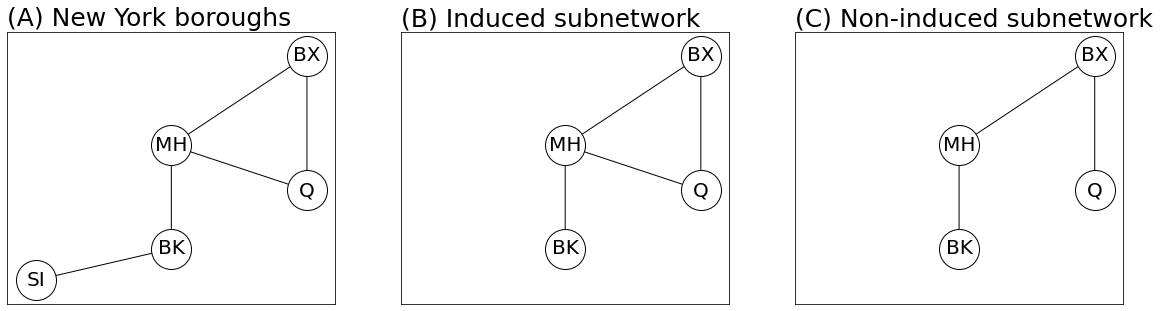
\includegraphics[width=\linewidth]{representations/ch4/Images/subnet.png}
    \caption[New York boroughs example]{\textbf{(A)} The New York Borough example. \textbf{(B)} The subnetwork induced by the node set \{BX, MH, Q, BX\}. This is also the example that we used to study clustering. \textbf{(C)} A subnetwork that is not an induced subnetwork.}
    \label{fig:ch4:subnet}
\end{figure}

\paragraph*{Representing subnetworks}
Notice that a subnetwork is a collection of nodes and edges defined on these nodes. Therefore, a subnetwork is itself also a network. This means that we could still represent a subnetwork using an adjacency matrix, with the caveat that the number of rows and columns might not be the same (since the nodes of a subnetwork are a subset of the nodes of the network) and the density might change (since the edges of a subnetwork are a subset of the edges of the network).

Let's think about why this matters.

\paragraph*{A caveat with the adjacency matrix of subnetworks}
Let's imagine that you have a simple network with the adjacency matrix $A$:
\begin{align*}
    A = \begin{bmatrix}
        0 & 0 & 0 \\
        0 & 0 & 1 \\
        0 & 1 & 0
    \end{bmatrix}
\end{align*}
And you consider a subnetwork that is induced by nodes \{2, 3\}. The induced subnetwork would have an adjacency matrix that looks like this:
\begin{align*}
    A_s = \begin{bmatrix}
        0 & 1 \\
        1 & 0
    \end{bmatrix}
\end{align*}
The key idea here is that, if you ignore the structure of the network when we do this, and conceptualize an induced subnetwork as a {deletion} of rows and columns, it becomes very difficult to figure out (later on in your analysis) which node is which. For instance, in your initial network, you might have also had a vector with $3$ elements (one for each node) that contained useful information about the nodes that you want to use later in your analysis. If you discard which nodes were included in your subnetwork, it will be very difficult (later in the analysis) to decipher which node is associated with which piece of information in your vector. For this reason, whenever you compute a subnetwork, we would {strongly} recommend that you make a note of it somewhere and store the nodes from the initial network that were retained in the subnetwork, so that you don't end up confused later on.

A particular induced subnetwork that you will often be concerned with is known as the largest connected component (LCC). 


\subsubsection{The largest connected component (LCC) is the largest subnetwork of connected nodes}
\label{sec:ch4:prop-net:lcc}
To define the largest connected component, we'll need to modify our example slightly. Let's say your network also includes the Boston area, and you have two new nodes, Boston (BO) and Cambridge (CA). Boston and Cambridge have several bridges between one another, so an edge exists between them. However, there are no bridges between boroughs of New York and the Boston area, so there are no edges from nodes in the Boston area to nodes in the New York area. Let's see how we would add this programmatically:

\begin{lstlisting}[style=python]
G_withbos = deepcopy(G)
G_withbos.add_node("BO", pos=(8, 6))
G_withbos.add_node("CA", pos=(8, 8))
G_withbos.add_edge("BO", "CA")
# fetch positions with boston and cambridge added
pos = nx.get_node_attributes(G_withbos, 'pos')
# plot
nx.draw_networkx(G_withbos, with_labels=True, node_color="black", pos=pos,
                font_color="white", edge_color="black")
\end{lstlisting}

We visualize the network with Boston and Cambridge in Figure \ref{fig:ch4:lcc}(A). 

The entire network can be described by the sets:
\begin{enumerate}
    \item $\mathcal V = \{SI, MH, BK, BX, Q, CA, BO\}$, and
    \item $\mathcal E = \{(SI, BK), (MH, BK), (MH, Q), (MH, BX), (MX, Q), (CA, BO)\}$.
\end{enumerate}

Notice that you have two distinct sets of nodes, those of New York and those of Boston, which are {only} connected amongst one another. Formally, these two sets of nodes can be described as inducing {connected components} of the network topology $(\mathcal V, \mathcal E)$. A \textit{connected component} is an induced subnetwork in which any two nodes are connected to each other by a path through the network. The two connected components are the New York induced subnetwork:

\begin{enumerate}
    \item The nodes $\mathcal V_N$: $\{SI, BK, Q, MH, BX\}$, and
    \item The edges $\mathcal E_N$: $\left\{(SI, BK), (BK, MH), (MH, Q), (MH, BX), (Q, BX)\right\}$.
\end{enumerate}

and the Boston induced subnetwork:
\begin{enumerate}
    \item The nodes $\mathcal V_B$: $\{CA, BO\}$, and
    \item The edges $\mathcal E_B$: $\left\{(CA, BO)\right\}$.
\end{enumerate}

We plot each individually in Figure \ref{fig:ch4:lcc}(B) and Figure \ref{fig:ch4:lcc}(C). If the network and the largest connected component are equivalent, we can omit the term {component}, and just say that the network is \textit{connected}.

\begin{figure}[h]
    \centering
    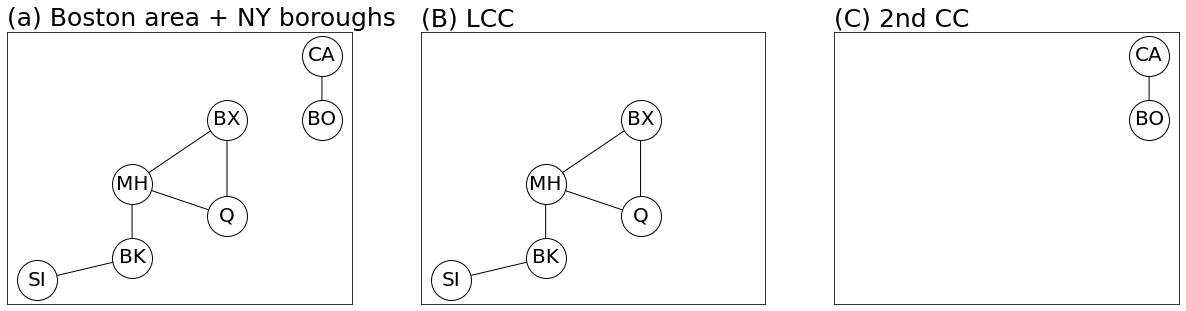
\includegraphics[width=\linewidth]{representations/ch4/Images/lcc.png}
    \caption[Connected Components]{\textbf{(A)} shows the New York boroughs with the added nodes for Boston and Cambridge. \textbf{(B)} shows the connected component induced by the boroughs of New York, which is also the LCC. \textbf{(C)} shows the connected component induced by Boston and Cambridge.}
    \label{fig:ch4:lcc}
\end{figure}
The \textit{largest connected component} (LCC) of a network is the connected component with the most nodes. In your example, the New York connected component has five nodes, whereas the Boston connected component has two nodes. Therefore, the New York connected component is the LCC of this simple network. You can compute the connected components and plot the largest connected component using \texttt{networkx} like this:

\begin{lstlisting}[style=python]
# returns a list of connected components, ordered 
# by decreasing size (#nodes)
cc_withbos = nx.connected_components(G_withbos)
# return the connected components, as networks
CC_nets = [G_withbos.subgraph(cc).copy() for cc in cc_withbos]

# plot the LCC
nx.draw_networkx(CC_nets[0], with_labels=True, node_color="black", pos=pos,
                font_color="white", edge_color="black")
\end{lstlisting}

A lot of times, when you are dealing with networks, they might already be in adjacency matrices. You can pass adjacency matrices directly into \texttt{graspologic} to obtain a LCC using:
\begin{lstlisting}
from graspologic.utils import largest_connected_component as lcc

A_withbos = nx.to_numpy_array(G_withbos)
A_lcc, retained_nodes = lcc(A_withbos, return_inds=True)
\end{lstlisting}
This is one of the {easiest} times for the caveat that we mentioned about subnetworks to arise. The \texttt{return\_inds} argument returns the rows/columns of \texttt{A\_withbos} that were retained for the LCC. The default functionality is to {not} return these indices, so proceed with caution!

\subsubsection{Connected components in directed networks}

The \textit{largest connected component} (LCC) of a network is the connected component with the most nodes. In your example, the New York connected component has five nodes, whereas the Boston connected component has two nodes. Therefore, the New York connected component is the LCC of this simple network.

Like the degree compared to the in- and out- degrees, for directed networks, connected components for directed networks need to be defined a little bit differently. A directed subnetwork is \textit{strongly connected} if directed paths exist between every pair of nodes in the subnetwork. 

A directed subnetwork is \textit{weakly connected} if the underlying directionalities are ignored, and the resulting undirected subnetwork is a connected component. Figure \ref{fig:ch4:directed}(C) shows an example of a strongly connected network, because you can travel along a path from each node to every other node in the network. On the other hand, Figure \ref{fig:ch4:directed}(B) shows an example of a weakly connected component when the bridge from MH to BK is out of service. This is because there is no longer a way to follow a path from SI or BK to MH, Q, and BX. When we ignore the arrows entirely, the resulting undirected network is still connected, as shown in Figure \ref{fig:ch4:directed}(A).


\newpage
\section{Types of network representations}
\label{sec:ch4:net-rep}

Now that you know how to represent networks with matrices and have some ideas of properties of networks, let's take a step back and take a look at what network representation is in general, and the different ways you might think about representing networks to understand different aspects of the network.

We already know that the topological structure of networks is just a collection of nodes, with pairs of nodes potentially linked together by edges. Mathematically, this means that a network is defined by two objects: the set of nodes, and the set of edges, with each edge just being defined as a pair of nodes for undirected networks. Networks can have additional structure: you might have extra information about each node (``features'' or ``covariates''), which we'll talk about when we cover Joint Representation Learning in Section \ref{ch6:joint}. Edges might also have weights, which are usually measure the connection strength in some way. We learned in the previous section that network topology can be represented with matrices in a number of ways -- with adjacency matrices, Laplacians, or (less commonly) with incidence matrices. 

One major challenge in working with networks is that a lot of standard mathematical operations and metrics remain undefined. What does it mean to add a network to another network, for instance? How would network multiplication work? How do you divide a network by the number 6? Without these kinds of basic operations and metrics, you are left in the dark when you try to find analogies to non-network data analysis.

Another major challenge has to do with the nature of network data. As it turns out, for any given number of nodes, there are a finite number of possible networks. When you have a finite number of possible outcomes, one of the most natural approaches is to attempt to use the data to try to describe each possible outcome individually. For instance, if you are flipping a coin, you might try to use the data (coin flips that you see) to determine with which probability the coin lands on heads or tails, since heads and tails are the two possible outcomes of the coin flip.

Unfortunately, we cannot possibly do this for network data. When a simple network has $n$ nodes, the number of possible networks that you could observe is $2^{\binom n 2}$ (we will derive this result later in Section \ref{sec:ch5:er}). We plot what this looks like in Figure \ref{fig:ch4:nnets}. When you allow for only 50 nodes, there are already more than $10^{350}$ possible networks. Just for reference, it is estimated that there are $10^{80}$ atoms in the known universe. If you created $10^{80}$ new universes, each with $10^{80}$ atoms, the total number of atoms across all universes would still be nowhere near this amount. 

In this section, we will explore the ways in which we conceptualize network representations to overcome this limitation. This section will prepare you to conceptualize the many particular strategies that you will learn later in Chapters \ref{sec:ch5} and \ref{sec:ch6}.

\begin{figure}[h]
    \centering
    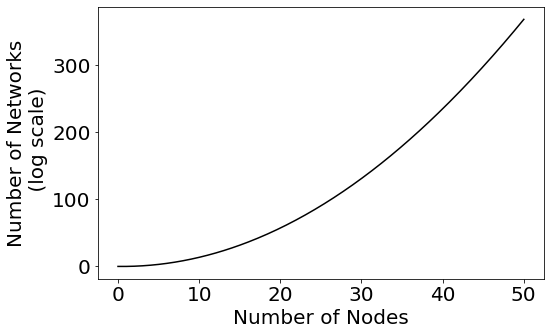
\includegraphics[width=0.7\linewidth]{representations/ch4/Images/nnets.png}
    \caption[Number of networks for $n$ nodes]{The number of possible distinct networks that you could have for a given number of nodes.}
    \label{fig:ch4:nnets}
\end{figure}

\subsection{Bag of Features}

The first approach is called the bag of features. The idea is that you take networks and you compute statistics from them, either for each node or for the entire network. These statistics could be simple things like the edge count or average path length between two nodes like you learned about in the last section, or more complicated metrics like the modularity {cite:p}`Newman2006Jun`, which measures how well a network can be separated into communities. Unfortunately, network statistics like these tend to be correlated; the value of one network statistic will almost always influence the other. This means that it can be difficult to interpret analysis that works by comparing network statistics. It's also hard to figure out which statistics to compute, since there are an infinite number of them.

\subsubsection{You Lose A Lot of Information with the Bag of Features Approach}

Let's take a look at a collection of networks in Figure \ref{fig:ch4:anascombe}:

\begin{figure}[h]
    \centering
    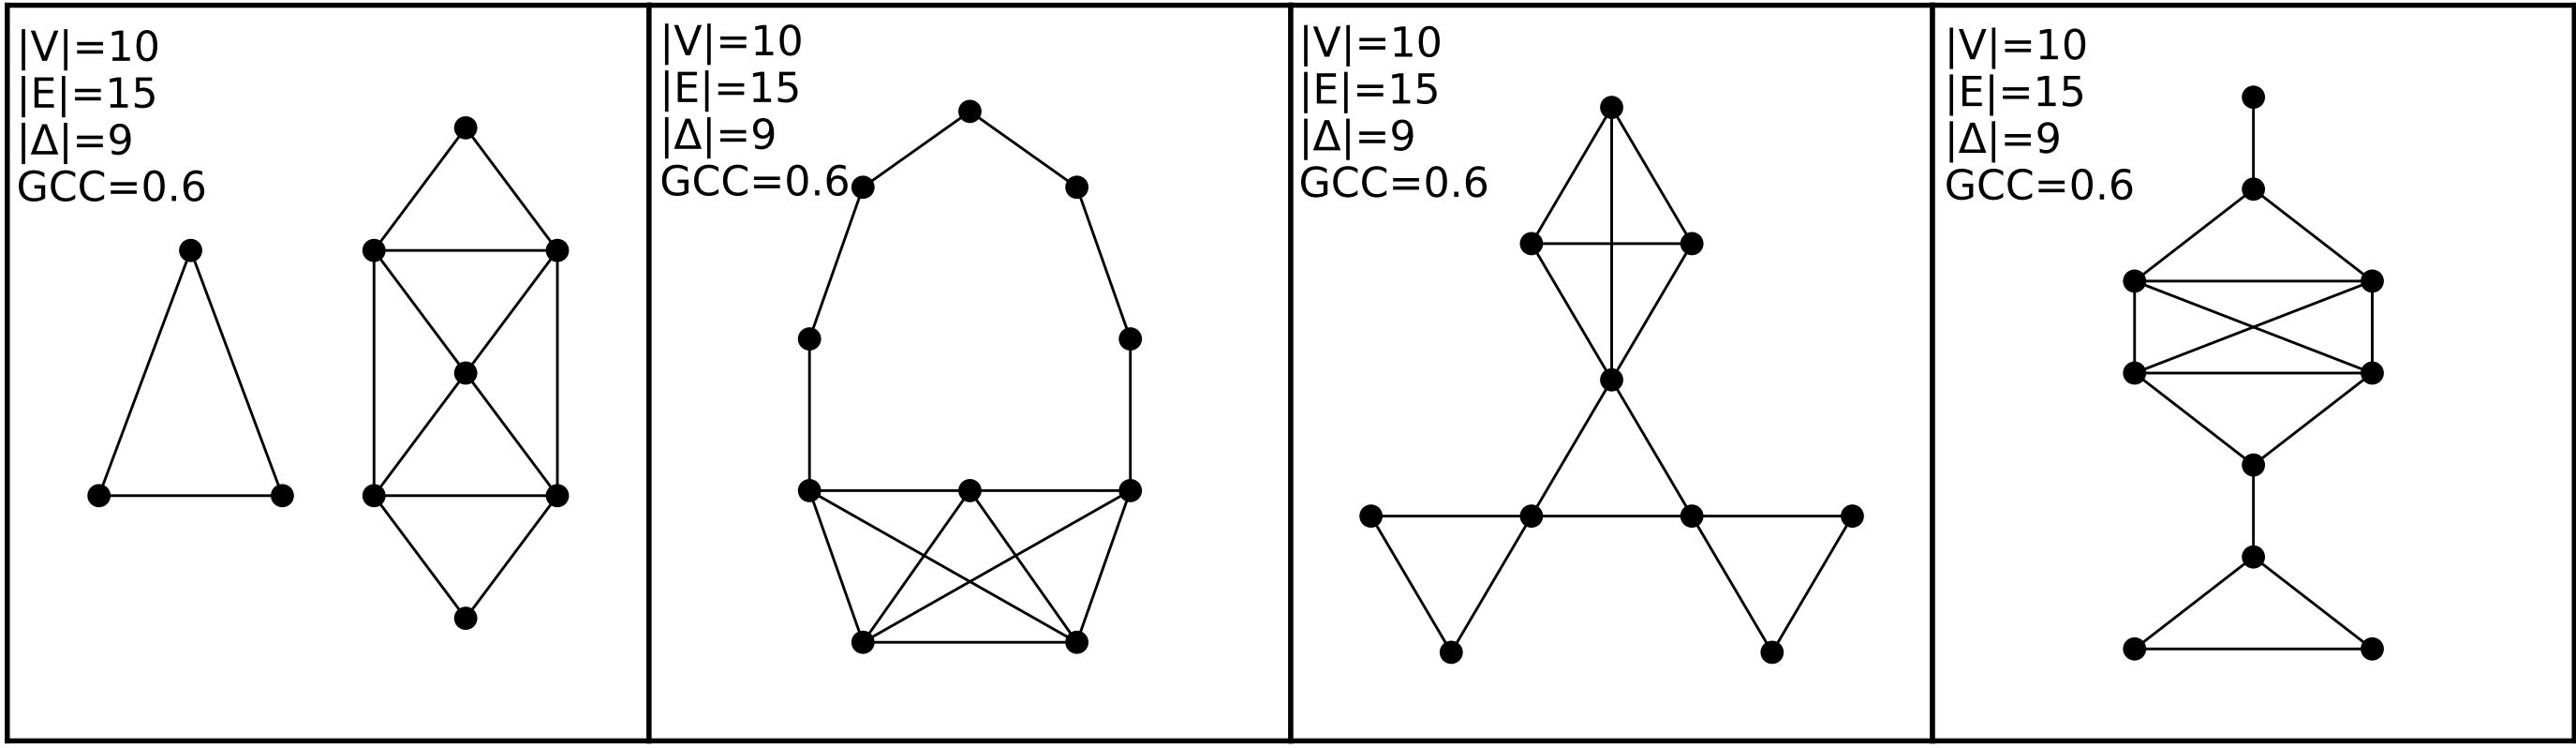
\includegraphics[width=\linewidth]{representations/ch4/Images/anascombe.jpeg}
    \caption[Very different networks can have the same summary statistics]{Four networks, all of which have the exact same network statistics for the four statistics we show here. They each have ten nodes and 15 edges. They also all contain the same number of closed triangles, and the same global clustering coefficient from Section \ref{sec:ch4:prop-net:clustering}.}
    \label{fig:ch4:anascombe}
\end{figure}

Each of these networks, however, are completely different from each other. The first network, for instance, has two connected components, while the others are all connected. The second network has a community of nodes that are only connected along a path, and a different community which are tightly connected, and so on. Modeling these networks through computing these features from them would lose a great deal of useful information about the topology of the network.


\paragraph{Network Features Tend to be Correlated}
\label{sec:ch4:net-rep:featurelims}

As we mentioned in the last paragraph, if you consider all possible networks, knowing the value of any of the network features gives you information about what the value of other network features might be.

Let's play around with this. We'll make $100$ random networks, each with $50$ nodes, and then we'll compute some common network statistics that people use in practice. Then, we'll look at how correlated these features are. For now, just think of a random network as being a network with each node being connected to each other node with some set probability. Each network will have a different connection probability. These networks will also have communities --- groups of nodes which have similar connection probabilities of being connected with other groups of nodes. 

Conceptually, you could think about a particular type of community structure using the bridge example that we covered previously when we talked about the Boston and New York boroughs in the LCC example in Section \ref{sec:ch4:prop-net:lcc}. It is probably more likely that two boroughs that are in the same state have a bridge between them then two boroughs in totally different states, right? When you generate data later on in this book, we'll get into different types of network models you can use. You don't need to have too good of an idea of what the below simulation code is doing just yet --- we will go into more depth in Chapter \ref{sec:ch5}.

\begin{lstlisting}[style=python]
from graspologic.simulations import sbm
import numpy as np
from numpy.random import uniform

n_nodes = 50
n_networks = 100
np.random.seed(1234)
# within-community probability
p = uniform(size=100, low=.5).round(2)
# between-community probability
q = uniform(size=100, high=.5).round(2)

networks = []
for i in range(n_networks):
    np.random.seed(1234)
    P = np.array([[p[i], q[i]],
                  [q[i], p[i]]])
    network = sbm(n=[n_nodes//2, n_nodes//2], p=P)
    networks.append(network)
\end{lstlisting}
Now, for each of these networks, we'll calculate a set of network features, using some of the various properties you learned about in the previous Section \ref{sec:ch4:prop-net}.

The only new statistic that we will look at is known as the network \textit{modularity}. You don't need to know too much about this statistic right now, other than the fact that it quantifies how much ``stronger'' the within-community effect is than the between-community effect (basically, that idea we described that New York boroughs would be more likely to have a bridge to other New York boroughs, than with either of the two cities in Massachusetts). The other statistics that we will compute will be the network density, the clustering coefficient, and the path length, all of which we discussed in Section \ref{sec:ch4:prop-net}.

The code below defines functions to calculate each of these network features, and then calculates them for each of the networks you created above.

We'll also define a preprocessing decorator, which just converts the network from a numpy array into the format networkx uses.


\begin{lstlisting}[style=python]
import functools
import networkx as nx

def preprocess(f):
    @functools.wraps(f)
    def wrapper(network):
        network = nx.from_numpy_matrix(network)
        return f(network)
    return wrapper

@preprocess
def modularity(network):
    communities = nx.algorithms.community.greedy_modularity_communities(network)
    Q = nx.algorithms.community.quality.modularity(network, communities)
    return Q

@preprocess
def network_density(network):
    return nx.density(network)

@preprocess
def clustering_coefficient(network):
    return nx.transitivity(network)

@preprocess
def path_length(network):
    if nx.number_connected_components(network) != 1:
        # You want to make sure this still works if your network isn't fully connected!
        network = max((network.subgraph(c) for c in nx.connected_components(network)), 
                      key=len)
    return nx.average_shortest_path_length(network)
\end{lstlisting}

Now, we'll calculate all of these features for each network, and finally we'll create a heatmap of their correlation.

\begin{lstlisting}[style=python]
import pandas as pd

network_features = []
for i, network in enumerate(networks):
    modularity_ = modularity(network)
    network_density_ = network_density(network)
    clustering_coefficient_ = clustering_coefficient(network)
    path_length_ = path_length(network)
    features = {"Modularity": modularity_, "Network Density": network_density_, 
                "Clustering Coefficient": clustering_coefficient_, "Average Path Length": path_length_}
    network_features.append(features)
    
df = pd.DataFrame(network_features)
feature_correlation = df.corr()
\end{lstlisting}
We show the results of this plot in Figure \ref{fig:ch4:anascombe}. Numbers close to 1 mean that when the first feature is large, the second tends to be large, numbers close to 0 mean that the features are not very correlated, and numbers close to -1 mean that when the first feature is large, the second feature tends to be small. 

\begin{figure}[h]
    \centering
    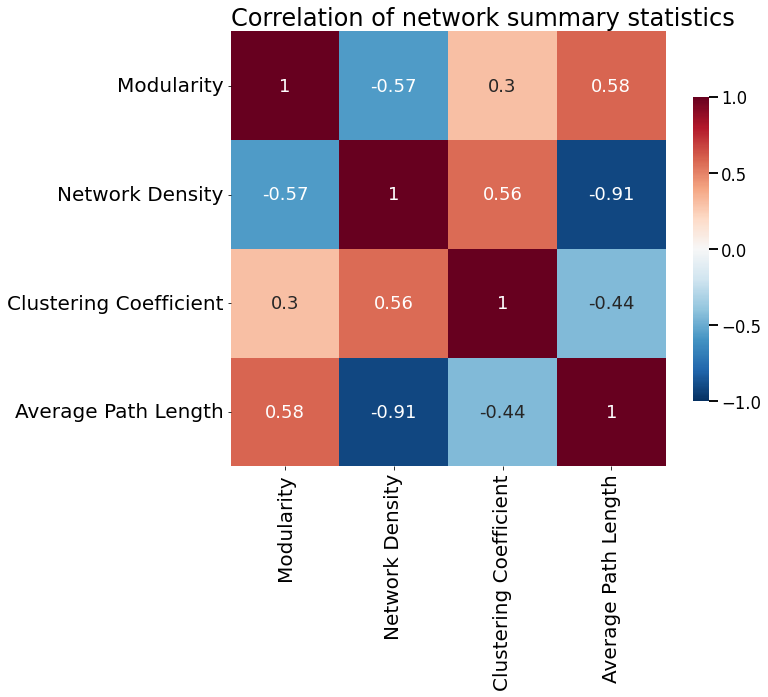
\includegraphics[width=0.8\linewidth]{representations/ch4/Images/corr.png}
    \caption[Correlation of netework features experiment]{The networks tend to exhibit correlation across various summary statistics. Note that none of the correlations are particularly close to $0$, and some (such as path length and density) are nearly perfectly correlated/anti-correlated.}
    \label{fig:ch4:corr}
\end{figure}

If you're familiar with correlation, that these numbers aren't particularly close to zero means that many of the features contain varying degrees of information about other features. Some of these features being big might say that another feature tends to also be high (positive correlation). Some of these features being big might say that another feature might tend to be the small (negative correlation). Some of these features don't tell you much about another particular feature (for instance, clustering and modularity only have a correlation with a magnitude around $0.3$), and some features are nearly perfectly informative about other features (network density and average path length are nearly perfectly negative-correlated with a value of $-.91$; that is, a high average path length implies a low network density, and vice versa). 

\paragraph{Why Network Feature Correlatedness Can Lead To Problems}

Let's take a step back to the implications of using the bag of features approach to analyze networks, now that you can see how correlated they usually are. Say you have a bunch of brain networks of mice, where the nodes are neurons and the edges are connections between neurons. You have a group of mice who were raised total darkness, and another group who were raised normally: let's call the ones who were raised in the darkness the batman mice. You're interested in how the visual parts of the brain are affected in the batman mice. You find the networks for only the visual parts of their brain, and then you calculate some network feature; maybe the density. It turns out that the network density is much lower for batman mice than it is for normal mice, so you conclude that raising mice in the darkness causes lower network density. Seems reasonable.

The problem is that network density is correlated with pretty much every other network feature you could have used. When you perform science, a primary focus of science tends to be establishing \textit{causality}. While we won't go much into causality here (there is an entire field dedicated to just this topic, called {causal inference}  for which there are many stellar reference texts), the jist is this. When you try to establish causality, you want to show a cause and effect type of relationship: the presence, or lack thereof, of some item $X$ {causes} an outcome $Y$ to happen. Whenever you do science, you want to find the root causes of {why} something is what it is: a mental illness is caused by a misfiring neuron, a misfolded protein is caused by the absence of a particular amino acid, a pair of friends having a major fight led to the students in a school being separated friendship wise into two distinct groups of people who support one student or the other. What you don't want to do is find something that just happens to be {correlated} with the thing that is impacted. 

For an example of this, we'll rotate back to our example from Section \ref{sec:ch1:howstudy:wontdiscuss}. If all smokers were older people and all non-smokers were younger people, just observing that the smokers tended to have higher rates of lung cancer would be insufficient to conclude whether smoking, or aging, cause lung cancer. Fortunately, statisticians found a way out: they took large groups of people with similar age ranges (and a number of other factors), and showed that the smokers had higher cancer rates (thus, ``untangling'' the correlatedness of age and smoking status). 

When you look at network features as things that potentially ``cause'' a particular effect, you can't really ``untangle'' the correlatedness of these network features, and it becomes extremely difficult, if not {impossible}  to actually establish which aspects of the network topology are actually causing or effected by the factor you are studying. 

For this reason, we think that network features are useful to {ascertain} whether something has an effect on the network, and provide information as to which directions you might want to look to establish causality. However, network features alone are insufficient, in our opinion, for defining causality. 

\subsection{Bag of Edges}
\label{sec:ch4:net-rep:bagofedges}

The second approach to studying networks is called the bag of edges. Here, you just take all of the edges in your network and treat them all as independent entities. You study each edge individually, ignoring any interactions between edges. This can work in some situations, but you still run into dependence: if two people within a friend group are friends, that can change the dynamic of the friend group and so change the chance that a different set of two people within the group are friends.

More specifically, in the bag of edges approach, you generally assume that every edge in your network will exist with some particular {probability} which can be different depending on the edge that you're looking at. For example, there might be a 60\% chance that the first and second nodes in your network are connected, but only a 20\% chance that the third and fourth nodes are. What often will happen here is that you have multiple networks describing the same (or similar) systems. For example, let's use the mouse example again from above. You have your batman mice (who were raised in the dark) and your normal mice. You'll have a network for each batman mouse and a network for each normal mouse, and you assume that, even though there's a bit of variation in what you actually see, the {probability} of an edge existing between the same two nodes is the same for all batman mice. Your goal would be to figure out which edges have a different {probability} of existing with the batman mice compared to the normal mice.

Let's make some example networks to explore this. We'll have two groups of networks, and all of the networks will have only three nodes for simplicity's sake. Each group will contain 20 networks, for a total of 40 networks. In the first group, every edge between every pair of nodes simply has a 50\% chance of existing. In the second group, the edge between nodes 0 and 1 will instead have a 90\% chance of existing, but every other edge will still just be 50\%. We'll generate ten networks from the first group, and ten networks from the second group.

\begin{lstlisting}[style=python]
from graspologic.simulations import sample_edges

P1 = np.array([[.5, .5, .5],
               [.5, .5, .5],
               [.5, .5, .5]])

P2 = np.array([[.5, .9, .5],
               [.9, .5, .5],
               [.5, .5, .5]])

# First group
n_networks = 20
networks = np.empty((2*n_networks, 3, 3))
for i in range(n_networks):
    networks[i,:,:] = sample_edges(P1)

# Second group
for i in range(n_networks, 2*n_networks):
    networks[i,:,:] = sample_edges(P2)

ys = np.array([1 for i in range(0, n_networks)] + [2 for i in range(0, n_networks)])
\end{lstlisting}

\subsubsection{Figuring out which edge is the signal edge}

By design, you know that the edge between nodes 0 and 1 has signal - the probability that it's there changes depending on whether your network is in the first or the second group. One common goal when using the bag of edges approach is finding signal edges: edges whose probability of existing changes depending on which type of network you're looking at. In your case, we're trying to figure out (without using your prior knowledge) that the edge between nodes 0 and 1 is a signal edge.

To find the outlier edge, you'll first get the set of all edges, along with their indices. Since all of your networks are undirected, you'll get the edges and their indices by finding all of the values in the the upper-triangular portion of the adjacency matrices.

\begin{lstlisting}[style=python]
edge_indices = np.triu_indices(3, k=1)
\end{lstlisting}

Now, you'll use a hypothesis test called the {Fisher's Exact Test} to find the outlier edge. You don't need to worry too much about what fisher's exact test is; here it is just something that will let us quantify whether an edge is different between the two groups, while makes limited assumptions about your data. We'll talk more about it in Section \ref{sec:ch9:ssn_incoherent}. 

In the code below, we:
\begin{enumerate}
    \item Loop through the edge indices,
    \item Get a list of all instances of that edge in the first group, and all instances of that edge in the second group, and
    \item Feed that list into the Fisher's exact test and obtain $p$-values (small $p$-value = more signal).
\end{enumerate}

\begin{lstlisting}[style=python]
from scipy.stats import fisher_exact

edge_pvals = []
for i, j in zip(*edge_indices):
    gr1_edge = networks[ys == 1,i,j].sum()  # number of group1 with edge i,j
    gr2_edge = networks[ys == 2,i,j].sum()  # number of group2 with edge i,j
    gr1_noedge = n_networks - gr1_edge  # number of group1 without edge i,j
    gr2_noedge = n_networks - gr2_edge  # number of group2 without edge i,j
    
    edge_tab = np.array([[gr1_edge, gr2_edge], [gr1_noedge, gr2_noedge]])  # arrange as in table
    
    edge_pvals.append(fisher_exact(edge_tab).pvalue)
\end{lstlisting}
You can see below that the $p$-value for the first edge, the one that connects nodes 0 and 1, is extremely small, whereas the $p$-values for the other two edges are relatively large.

\begin{lstlisting}[style=python]
np.array(edge_pvals).round(3)
\end{lstlisting}

\subsection{Bag of Nodes}
\label{sec:ch4:net-rep:bagofnodes}

Similarly to the bag of edges, you can treat all of the nodes as their own entity and do analysis on a bag of nodes. Much of this book will focus on the bag of nodes approach, because we'll often use edge count, covariate information, and other things when we work with bags of nodes. Although there's still correlation between nodes, it generally isn't as big of an issue. Most of the single-network methods you'll use in this book will take the bag of nodes approach. 

What we'll see repeatedly is that we take the nodes of a network and {embed} them so each node is associated with a point on a plot (this is called the {node latent space}). In a sense, this will ``tabularize'' our data, which as we learned in Section \ref{sec:ch1:challenges}, overcomes a major hurdle of network machine learning. Then, we can use other methods from mainstream machine learning to learn about our network. Deciding how to handle these ``bags of nodes'' will be a prime focus of Chapter \ref{sec:ch6}, and we will devote attention in Part \ref{p:app} to determining how we can use these bags of nodes.

We'll also often associate node representation with community investigation. The idea is that sometimes you have groups of nodes which behave similarly -- maybe they have a higher chance of being connected to each other, or maybe they're all connected to certain other groups of nodes. Regardless of how you define communities, a community investigation motif will pop up: you get your node representation, then you associate nearby nodes to the same community. We can then look at the properties of the node belonging to a particular community, or look at relationships between communities of nodes.

Since we'll use the bag of nodes approach heavily throughout this book, you'll be getting a much better sense for what you can do with it later. As a sneak preview right now, let's generate a few networks and embed their nodes to get a feel for what bag-of-nodes type analysis might look like. 

Don't worry about the specifics, but below you generate a simple network with two communities. Nodes in the same community have an 80\% chance of being connected, whereas nodes in separate communities have a 20\% chance of being connected. This is like saying that boroughs of New York \textit{or} boroughs near Boston have an 80\% of being connected by bridges, but boroughs of New York and boroughs near Boston have a 20\% chance of having a bridge between them. There are 20 nodes per community. Again, we'll cover the intuition of this particular generative model a lot more in Chapter \ref{sec:ch5}, so keep the big picture in focus for now.

\begin{lstlisting}[style=python]
from graspologic.simulations import sbm

# generate network
P = np.array([[.8, .2,],
              [.2, .8]])
network, labels = sbm(p=P, n=[20, 20], return_labels=True)
\end{lstlisting}

Now, you'll use graspologic to find the points in 2D space that each node is associated with. Again, don't worry about the specifics: this will be heavily explained later in the book. All you have to know right now is that we're {mapping} (transforming) the nodes of your network from network space, where each node is associated with a set of edges with other nodes, to the a tabular space, where each node is associated with an $x$-coordinate and a $y$-coordinate.

\begin{lstlisting}[style=python]
from graspologic.embed import AdjacencySpectralEmbed as ASE

ase = ASE(n_components=2)
embedding = ase.fit_transform(network)
\end{lstlisting}

Figure \ref{fig:ch4:bagonode} shows the result of this tabularization by community. Each of the dots in this plot is one of the nodes of your network. You can see that the nodes cluster into two groups: one group for the first community, and another group for the second community. Using this representation for the nodes of your network, you can open the door to later downstream machine learning tasks.

\begin{lstlisting}[style=python]
from graphbook_code import plot_latents, draw_cartesian, add_circle, text

ax = draw_cartesian(xrange=(-1, 1), yrange=(-1, 1))
plot = plot_latents(embedding, labels=labels, ax=ax)
plot.set_title("Bag of Nodes on a coordinate axis", y=1.1);

# plot circle
x_centroid, y_centroid = embedding[labels==0].mean(axis=0)
add_circle(x_centroid, y_centroid+.2, ax=ax)
ax.annotate("Nodes plotted \nas 2d points", xy=(x_centroid-.2, y_centroid+.2), xytext=(x_centroid-2, y_centroid), 
            arrowprops={"arrowstyle": "->"});
\end{lstlisting}
\begin{figure}[h]
    \centering
    \includegraphics[width=\linewidth]{representations/ch4/Images/bagonode.png}
    \caption{Nodes in the same community ending up being in similar areas of the $x$/$y$ coordinate axis above.}
    \label{fig:bagonode}
\end{figure}

\subsection{Bag of Networks}
\label{sec:ch4:net-rep:bagofnets}

The last approach is the bag of networks, which you'd use when you have more than one network that you're working with. Here, you'd study the networks as a whole and you'd want to test for differences across different networks or classify entire networks into one category or another. You might want to figure out the groups of networks look different, or whether you can learn information across all of the networks simultaneously. This is can be useful if you have many extremely large networks, with millions of nodes.

To showcase the bag of networks approach, let's create a few networks. We'll have one group of networks distributed the same way, and another group distributed differently. What you want to do is plot each network as a point in space, so that you can see the communities of networks directly.

Both sets of networks will have two communities of nodes, but the first set will have slightly stronger within-community connections than the second. Each network will have 200 nodes in it, 100 for each community.

\begin{lstlisting}[style=python]
def make_network(*probs, n=100, return_labels=False):
    pa, pb, pc, pd = probs
    P = np.array([[pa, pb], 
                  [pc, pd]])
    
    return sbm([n, n], P, return_labels=return_labels)

n = 100
p1, p2, p3 = .12, .06, .03

first_group = []
for _ in range(6):
    network = make_network(p1, p3, p3, p1)
    first_group.append(network)
    
second_group = []
for _ in range(12):
    network = make_network(p2, p3, p3, p2)
    second_group.append(network)
\end{lstlisting}

\begin{lstlisting}[style=python]
\end{lstlisting}
Again, don't worry too much yet about the process with which these networks were generated - that will all be explained in the next chapter. All you need to get out of this code is that you have six networks from the first group, and another twelve networks from the second. You can see these networks in heatmap form below. These networks are plotted in Figure \ref{fig:ch4:bagonets}(A). 

Now, you have to figure out some way of plotting each network as a point in space. Here's a rough overview for how you'll do it.

First, you'll take all of your networks and find a common space that you can orient all of the nodes into. The nodes for all of the networks will exist in the same space, meaning their locations can be compared with each other. We'll have a bunch of matrices, one for each network. Since each network has 200 nodes, and we're embedding into 2-dimensional space, we'll have six 200 by 200 matrices for the first group of networks, and another twelve 200 by 200 matrices for the second group. This process is called finding a {network} latent space with a homogeneous {node latent space}  and will be extremely valuable for embedding collections of networks later on. Again, this takes our collection of networks and \textit{tabularizes} them for us, taking each $200 \times 200$ adjacency matrix and turning it into a $200 \times 2$ matrix, effectively ``bagging the nodes'' like we did in the preceding section.

Next, once we have a bag of nodes for each network, we can use standard machine learning techniques with them. Here, we'll use classical multi-dimensional scaling (MDS), a popular dimensionality reduction technique. We'll do this by constructing a dissimilarity matrix which captures how dissimilar each ``bag of nodes'' is between every pair of networks, and then embed this dissimilarity matrix. This second embedding, in effect, tabularizes each network individually and gives us a bag of networks representation.

Again, don't worry if you don't understand the details: embedding and how it works will be explained in future chapters.

\begin{lstlisting}[style=python]
from graspologic.embed import OmnibusEmbed as OMNI
from graspologic.embed import ClassicalMDS

# Find a node latent space for the nodes of all of your networks
omni = OMNI(n_components=2)
omni_embedding = omni.fit_transform(first_group + second_group)

# embed each network representation into a 2-dimensional space
cmds = ClassicalMDS(2)
cmds_embedding = cmds.fit_transform(omni_embedding)

# Find and normalize the dissimilarity matrix
distance_matrix = cmds.dissimilarity_matrix_ / np.max(cmds.dissimilarity_matrix_)
\end{lstlisting}

You can see the dissimilarity matrix in Figure \ref{fig:ch4:bagonets}(B). As you can see, there look to be two groups of networks that tend to be quite similar amongst themselves, and quite different between the groups. The diagonals of the matrix are all 0, because the dissimilarity between a network and itself is 0.

Embedding this {new} matrix will give us a point in space for each network. Once you find the embedding for this dissimilarity matrix via MDS as above, you can plot each of the networks in space. Since there are six networks of the first type and twelve of the second type, one of the clusters has six dots, and the other has twelve dots. Let's take a look at this plot:
\begin{lstlisting}[style=python]
ax = draw_cartesian(xrange=(-1, 1), yrange=(-1, 1))
plot_latents(cmds_embedding, ax=ax, labels=labels)
\end{lstlisting}

\begin{figure}
    \centering
    \includegraphics[width=\linewidth]{representations/ch4/Images/bagonets.png}
    \caption[Bags of networks]{\textbf{(A)} the networks from each of the two groups. \textbf{(B)} The dissimilarity matrix between pairs of networks. \textbf{(C)} Each point represents a single network point in space. We can easily see the two clusters, which represent the two types of networks you created.}
    \label{fig:ch4:bagonets}
\end{figure}

\newpage
\section{Regularization}
\label{sec:ch4:regularization}

In practice, many networks you will encounter in network machine learning will not be simple networks: Many of the techniques we discuss will be just fine to use with weighted networks. Unfortunately, real world networks are often extremely noisy, and so the analysis of one real world network might not generalize very well to a similar real world network. For this reason, we turn to regularization. 

\textit{Regularization} is the process by which you either:
\begin{enumerate}
    \item Modify data for the purpose of mitigating overfitting due to idiosyncrasies of the observed data, and/or
    \item Modify the function you are estimating due to its fragility to the idiosyncracies of the observed data.
\end{enumerate}

In network machine learning, the first step of your analysis is to typically modify the network (or networks) themselves to allow better generalization of your statistical inference to new datasets. Later chapters will cover approaches in which you modify the function you are estimating.

For each of the following subsections, we'll pose an example, a simulation, and code for how to implement the desired regularization approach. It is important to realize that you might use several of these techniques simultaneously in practice, or you might have a reason to use these techniques that go outside of our working examples.

We start with a few running examples for this section. We have two non-simple networks:

\begin{floatingbox}[h]\caption{Activity/hobby network}
The nodes of this network are a group of $50$ area students, the first $25$ of whom are athletes, and the second $25$ are in marching band. To collect the first network, you ask each student to select from a list of $50$ school activities and outside hobbies that they enjoy. For a pair of students $i$ and $j$, the weight of their interest alignment will be a score between $0$ and $50$ indicating how many activities or hobbies that they have in common. 

We will refer to this network as the activity/hobby network. This network is undirected, since if student $i$ shares $x$ activities or hobbies with student $j$, then student $j$ also shares $x$ activities or hobbies with student $i$. This network is weighted, since the score is between $0$ and $50$. Finally, this network is loopless, because it would not make sense to look at the activity/hobby alignment of a student with themself, since every student would have perfect alignment of activities and hobbies with him or herself. 

Because the network is undirected, the researchers have only saved half the portion of the adjacency matrix that includes the entries $a_{ij}$ where $j > i$.
\end{floatingbox}

\begin{floatingbox}[h]\caption{Friendship network}
This network is collected using the same $50$ students as the activity/hobby network. To collect the second network, you ask each student to rate how good of friends they are with other students, on a scale from $0$ to $1$. A score of $0$ means they are not friends with the student or do not know the student, and a score of $1$ means the student is their best friend. We will refer to this network as the friendship network. This network is directed, since two students may differ on their understanding of how good of friends they are. This network is weighted, since the score is between $0$ and $1$. Finally, this network is also loopless, because it would not make sense to ask somebody how good of friends they are with themself.
\end{floatingbox}

Our scientific question of interest is how well activities and hobbies align with perceived notions of friendship. You want to use the networks of Examples 3.3 and 3.4 to learn about a hypothetical third network, whose nodes are identical to these two networks, but whose edges are whether the two individuals are friends (or not) on facebook. To answer this question, you have to do to some work to make your networks better suited to the task! We'll simulate some example networks, with output in Figure \ref{fig:ch4:friendex}.

\begin{lstlisting}[style=python]
from graspologic.simulations import sbm
import numpy as np

wtargsa = [[dict(n=50, p=.09), dict(n=50, p=.02)],
          [dict(n=50, p=.02), dict(n=50, p=.06)]]

wtargsf = [[dict(a=4, b=2), dict(a=2, b=5)],
          [dict(a=2, b=5), dict(a=6, b=2)]]

# activity network as upper triangle matrix
A_activity_uppertri = sbm(n=[25, 25], p=[[1,1], [1,1]], wt=np.random.binomial, wtargs=wtargsa, loops=False, directed=False)
A_activity_uppertri = np.triu(A_activity_uppertri)

# friend network
A_friend = sbm(n=[25, 25], p=[[.8, .4], [.4, 1]], wt=np.random.beta, wtargs=wtargsf, directed=True)
\end{lstlisting}

\begin{figure}[h]
    \centering
    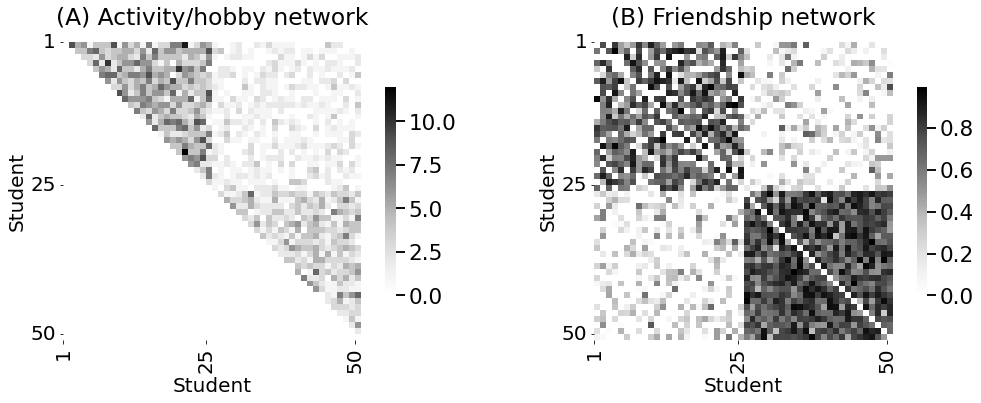
\includegraphics[width=\linewidth]{representations/ch4/Images/friendex.png}
    \caption[Friendship and activities networks]{A comparison of the two networks that we sampled to use in this section. The friendship network is shown in \textbf{(A)}, and the activity/hobby network is shown in \textbf{(B)}.}
    \label{fig:ch4:friendex}
\end{figure}

%% ALEX STOPPING POINT 07/02 4:36pm}

We'll also work with a third network which will have unique particularities from the preceding two, where we want to ask a question about only this network itself. 
\begin{floatingbox}[h]\caption{Unrelated business network}
The $17$ nodes in the network are local businesses, and an edge exists between a pair of businesses if they have business dealings with one another (they buy or sell products from/with the company). Three of these businesses operate in total exclusion and do not have any edges. Three of these businesses only work with one other business. One businesses work with all of the non-excluded businesses. 
\end{floatingbox}

To begin, we're going to start looking at the business network. Let's take a look at what this network looks like in Figure \ref{fig:ch4:businessex}.

\begin{lstlisting}[style=python]
from graphbook_code import heatmap
from matplotlib import pyplot as plt
from graspologic.simulations import er_np
import networkx as nx

n = 10
A_bus = er_np(n, 0.6)

# add pendants
n_pend = 3
A_bus = np.column_stack([np.row_stack([A_bus, np.zeros((n_pend, n))]), 
                         np.zeros((n + n_pend, n_pend))])

n = n + n_pend
# add pizza hut node
n_pizza = 1
A_bus = np.column_stack([np.row_stack([A_bus, np.ones((n_pizza, n))]), 
                         np.ones((n + n_pizza, n_pizza))])
n = n + n_pizza

# add isolates
n_iso = 3
A_bus = np.column_stack([np.row_stack([A_bus, np.zeros((n_iso, n))]), 
                         np.zeros((n + n_iso, n_iso))])
A_bus = A_bus - np.diag(np.diag(A_bus))
n = n + n_iso

# as a heatmap
node_names = [i for i in range(0, n)]
heatmap(A_bus.astype(int), title="Business Network Adjacency Matrix", 
               xticklabels=node_names, yticklabels=node_names)
# as a layout plot
G_bus = nx.from_numpy_matrix(A_bus)
node_pos = nx.shell_layout(G_bus)

plt.figure()
nx.draw(G_bus, pos=node_pos)
\end{lstlisting}

\begin{figure}[h]
    \centering
    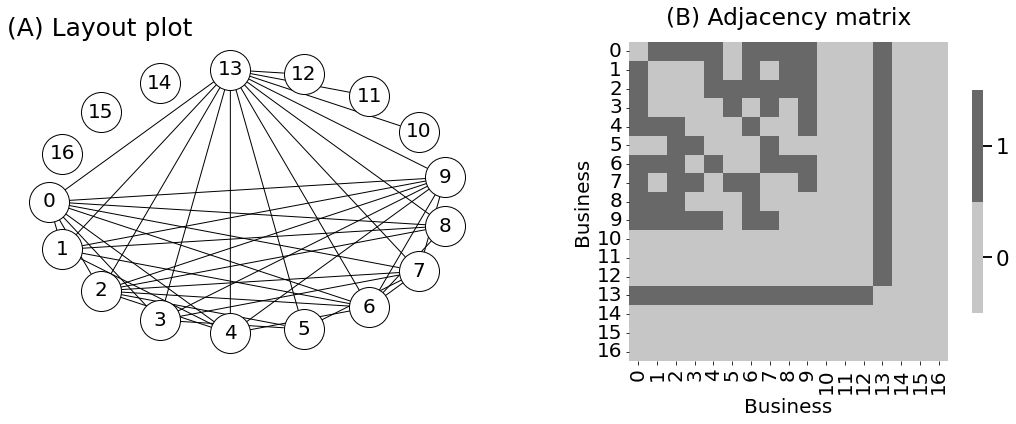
\includegraphics[width=\linewidth]{representations/ch4/Images/businessex.png}
    \caption[Business network example]{An example of a business network, where nodes are businesses and edges are whether the pairs of businesses have a business relationship.}
    \label{fig:ch4:businessex}
\end{figure}

\subsection{Node pruning}

Node pruning is a regularization technique in which you remove nodes for one reason or another. Typically, you will remove nodes due to some property about their degrees, or other properties (such as their \emph{connectedness} with other nodes that you care about). These strategies are covered loosely in the book \cite{Barabsi2013Mar}, and can be found in more computation-heavy network papers. Let's take a look at some of the strategies.

\subsubsection{Degree trimming removes nodes with unfavorable degrees}

In your business network, there are several nodes which tend to impart ``strange'' properties on downstream machine learning tasks. Some of these nodes, which include nodes with disproportionately high or low values, tend to yield numerical instability when you apply machine learning algorithms to them. By ``numerical instability'', what we mean is that the the (few) connections that nodes with low degrees have are going to have a disproportionately large impact on the machine learning task we perform. For this reason, it may be advantageous to remove nodes whose degrees are much different from the other nodes in the network. 

One special case of degree trimming is called removing \emph{isolates}. An \textit{isolated node} is a node which has a degree of $0$, meaning that it is not connected to any other nodes in the network. See if you can spot the isolates in Figure \ref{fig:ch4:businessex}.

Another special case of degree trimming is called the removal of \emph{pendants}. A \textit{pendant node} is a node which has a degree of $1$, meaning that it is only connected to one other node in the network. Try and see if you can spot the pendants in \ref{fig:ch4:businessex}.

You can remove isolates or pendants pretty simply. You simply need to compute the degree of each node in the network, and then retain the nodes with a degree \emph{above} your chosen threshold. To remove isolates, you would pick this threshold to be $0$ (retain nodes with non-zero degree), and to remove both pendants and isolates, you would pick this threshold to be $1$ (retain nodes with a degree exceeding $1$). You can do this like follows:
\begin{lstlisting}[style=python]
def compute_degrees(A):
    # compute the degrees of the network A
    # since A is undirected, you can just sum
    # along an axis.
    return A.sum(axis=1)

def prune_low_degree(A, return_inds=True, threshold=1):
    # remove nodes which have a degree under a given
    # threshold. For a simple network, threshold=0 removes isolates,
    # and threshold=1 removes pendants
    degrees = compute_degrees(A)
    non_prunes = degrees > threshold
    robj = A[np.where(non_prunes)[0],:][:,np.where(non_prunes)[0]]
    if return_inds:
        robj = (robj, np.where(non_prunes)[0])
    return robj

A_bus_lowpruned, nonpruned_nodes = prune_low_degree(A_bus)
\end{lstlisting}

Next, we'll plot the network as a layout plot. Remember how we told you in Section \ref{sec:ch4:prop-net:subnetwork} that if you just ``threw away'' nodes ignorant of which ones you threw away that you would run into trouble? Here's a good example of that. If you had just pruned the low degree nodes, you would have no idea which nodes were originally plotted \emph{where} in the initial layout plot that you looked at. Fortunately, since we included this information, we can recover the spatial position of each node pretty easily, and replot the network with the nodes that were not pruned in the same place that they were before:

\begin{lstlisting}[style=python]
node_names_lowpruned = [node_names[i] for i in nonpruned_nodes]
node_pos_lowpruned = {i : node_pos[j] for i, j in enumerate(nonpruned_nodes)}

G_bus_lowpruned = nx.from_numpy_matrix(A_bus_lowpruned)

nx.draw(G_bus_lowpruned, pos=node_pos_lowpruned)
\end{lstlisting}

The resulting layout plot is shown in Figure \ref{fig:ch4:nodeprune}(A).

\begin{figure}[h]
    \centering
    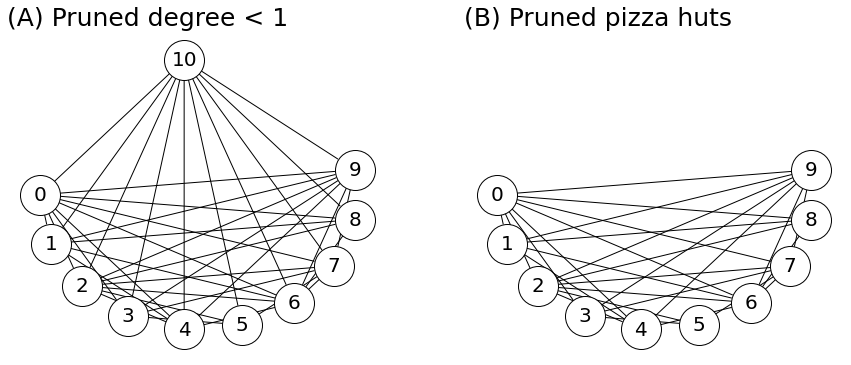
\includegraphics[width=\linewidth]{representations/ch4/Images/nodeprune.png}
    \caption[Pruning high and low degree nodes]{\textbf{(A)} The business network after pruning nodes with a degree less-than or equal to $1$, which consists of isolates and pendants. \textbf{(B)} The business network after pruning isolates and pendants followed by pizza-hut nodes.}
    \label{fig:ch4:nodeprune}
\end{figure}

A useful way to determine whether you have isolates or pendants is to look at the \emph{degree distribution histogram} of the network. The degree distribution histogram just shows a y axis of counts for a given range of possible x values. When the values you want a histogram for can only take a limited number of possible values, you might be able to get away with just looking at each possible value as its own x-axis point. Sometimes, when the values can take a large number of possible values, this might not be possible. You might have to \emph{bin} similar values together to make the plot appreciable. The degree distribution, before and after removing pendants/isolates, looks like this:

\begin{lstlisting}[style=python]
degrees_before = compute_degrees(A_bus)
degrees_after = compute_degrees(A_bus_lowpruned)
\end{lstlisting}

and can be plotted like this:

\begin{lstlisting}[style=python]
from seaborn import histplot
fig, axs = plt.subplots(1,2, figsize=(15, 4))

ax = histplot(degrees_before, ax=axs[0], binwidth=1, binrange=(0, 14))
ax.set_xlabel("Node degree");
ax.set_ylabel("Number of Nodes");
ax.set_title("Business Network, before pruning");
ax = histplot(degrees_after, ax=axs[1], binwidth=1, binrange=(0, 14))
ax.set_xlabel("Node degree");
ax.set_title("Business Network, after pruning")
\end{lstlisting}

\paragraph{Removing pizza hut nodes}

On the other end of the spectrum, it is often useful to remove nodes which don't really tell us anything about the network at all because they are just connected to \emph{everything}. We call these nodes \emph{pizza hut} nodes, because let's face it, pizza hut can be delivered pretty much anywhere! After pruning, we actually \emph{created} a pizza hut node, which you can see from low-degree pruned network in Figure \ref{fig:ch4:nodeprune}(A). 

We can prune these nodes just as easily as before. This time, note that our pruning threshold is simply set as the maximum possible node degree. Further, note that since we pruned the pizza-hut node from the low-pruned network, we need to recover which nodes from the original network were retained. This should further emphasize to you the importance of keeping track of your indices whenever you remove nodes from your network, as you can imagine that if you do a lot of node prunings, this can get confusing rapidly:

\begin{lstlisting}[style=python]
def prune_high_degree(A, return_inds=True, threshold=0):
    # remove nodes which have a degree over a given
    # threshold. For a simple network, threshold=A.shape[0] - 1
    # removes any pizza hut node
    degrees = compute_degrees(A)
    non_prunes = degrees < threshold
    robj = A[np.where(non_prunes)[0],:][:,np.where(non_prunes)[0]]
    if return_inds:
        robj = (robj, np.where(non_prunes)[0])
    return robj

# pruning nodes 
A_bus_pruned, highpruned_nodes = prune_high_degree(A_bus_lowpruned, threshold=A_bus_lowpruned.shape[0] - 1)

# get the nodes that aren't pruned by low pruning nor pizza hut node pruning
node_names_pruned = [node_names_lowpruned[i] for i in highpruned_nodes]
node_pos_pruned = {i : node_pos_lowpruned[j] for i, j in enumerate(highpruned_nodes)}

G_bus_retained = nx.from_numpy_matrix(A_bus_pruned)
nx.draw(G_bus_retained, pos=node_pos_pruned)
\end{lstlisting}
The result of both low-degree pruning (for isolates and pendants) and high-degree pruning (for pizza hut nodes) is shown in Figure \ref{fig:ch4:nodeprune}(B). 

Again, you might want to visualize the degree distribution plot to decide whether you want to prune nodes with high degrees.

\subsubsection{The Largest Connected Component is the largest subnetwork of connected nodes}

Two sections ago in Section \ref{sec:ch4:prop-net:lcc}, you learned about computing the largest connected component. This is a node pruning technique, because it "throws out" all of the nodes other than the ones which are in the largest connected component. We would encourage you to go back through this example now if you have time, so that you will better associate it as a regularization technique in your brain.


\subsection{Regularizing the edges of unweighted networks}

\subsubsection{Symmetrizing the adjacency matrix gives us undirectedness}
\label{sec:ch4:regularization:symmetrize}
If you wanted to learn from the friendship network about whether two people shared similar hobbies/activities, a reasonable first place to start might be to \emph{symmetrize} the friendship adjacency matrix. The activity/hobby network is \emph{undirected}, which means that if a student $i$ is friends on facebook with student $j$, then student $j$ is also friends with student $i$. On the other hand, as you learned above, the friendship network was directed. Since your question of interest is about an undirected network but the network you have is directed, it might be useful if you could take the directed friendship network and learn an undirected network from it. This relates directly to the concept of \emph{interpretability}, in that you need to represent your friendship network in a form that will produce an answer for us about your facebook network which you can understand.

Another reason you might seek to symmetrize the friendship adjaceny matrix is that you might think that asymmetries that exist in the adjacency matrix are just \emph{noise}. You might assume that the adjacency entries $a_{ij}$ and $a_{ji}$ relate to one another, so together they might be able to produce a single summary number that better summarizes their relationship all together. 

As a final reason, you might think that the asymmetries are meaningful, but that they \emph{are not feasible to consider}. Many statistical models for networks, and many techniques developed to analyze networks, might only have interpretations for undirected networks. This means that if you want to use these techniques, you might have to settle for making your network undirected first. 

There are many other reasons you might want undirected networks, these are just a small subset of the reasons.

Jargon wise, remember that in a symmetric matrix (for an undirected network), $a_{ij} = a_{ji}$, so in an \emph{asymmetric} matrix (for a directed network), $a_{ij} \neq a_{ji}$. To symmetrize the friendship network, what you want is a \emph{new} adjacency value, which we will call $w_{ij}$, which will be a function of $a_{ij}$ and $a_{ji}$. Then, you will construct a new adjacency matrix $A'$, where each entry $a_{ij}'$ \emph{and} $a_{ji}'$ are set equal to $w_{ij}$.  The little apostrophe just signifies that this is a potentially different value than either $a_{ij}$ or $a_{ji}$. Note that by construction, $A'$ is in fact symmetric, because $a_{ij}' = a_{ji}'$ due to how you built $A'$. For this matrix, we'll look at a generic adjacency matrix that looks like this:

\begin{align*}
    A &= \begin{bmatrix}
        a_{11} & {a_{12}} & {...} & {a_{1n}} \\
        {a_{21}} & \ddots & {\ddots} & {\vdots} \\
        {\vdots} &{\ddots} &\ddots & {a_{n-1, n}}\\
        {a_{n1}} & {...} & {a_{n,n-1}} & a_{nn}
    \end{bmatrix},
\end{align*}

\paragraph{Ignoring a ``triangle'' of the adjacency matrix}

The easiest way to symmetrize a network $A$ is to just ignore part of it entirely. In the adjacency matrix $A$, you will remember that you have an upper and a lower triangular part of the matrix. For instance, the upper triangle looks like this:

\begin{align*}
    \Delta &= \begin{bmatrix}
        0 & {a_{12}} & {...} & {a_{1n}} \\
        {0} & \ddots & {\ddots} & {\vdots} \\
        {\vdots} &{\ddots} &\ddots & {a_{n-1, n}}\\
        {0} & {...} & {0} & 0
    \end{bmatrix}.
\end{align*}
This is called the \emph{upper triangle} because if you look at the non-zero entries, they form a triangular shape in the matrix when the matrix is in its row/column orientation like this. Note this matrix is identical to $A$ for any row $i$ and column $j$ where $j > i$, but is equal to $0$ for any entries where $j \leq i$. The transpose of this matrix is:
\begin{align*}
    \Delta^\top &= \begin{bmatrix}
        0 & {0} & {...} &{0}\\
        {a_{12}}& \ddots & {\ddots} & {\vdots} \\
        {\vdots}&{\ddots} & \ddots & {0} \\
        {a_{1n}}&{...} &{a_{n-1,n}} & 0
    \end{bmatrix}.
\end{align*}
So when we add the two together, we get this:
\begin{align*}
    \Delta + \Delta^\top &= \begin{bmatrix}
        0 & {a_{12}} & {...} & {a_{1n}} \\
        {a_{12}} & \ddots & {\ddots} & {\vdots} \\
        {\vdots}&{\ddots} &\ddots & {a_{n-1, n}}\\
        {a_{1n}}&{...} &{a_{n-1,n}} & 0
    \end{bmatrix}.
\end{align*}
You're almost there! You just need to add back the diagonal of $A$, which you will do using the matrix $diag(A)$ which has values $diag(A)_{ii} = a_{ii}$, and $diag(A)_{ij} = 0$ for any $i \neq j$:
\begin{align*}
    A' &= \Delta + \Delta^\top + diag(A) = \begin{bmatrix}
        a_{11} & {a_{12}} & {...} & {a_{1n}} \\
        {a_{12}} & \ddots & {\ddots} & {\vdots} \\
        {\vdots}&{\ddots} &\ddots & {a_{n-1, n}}\\
        {a_{1n}}&{...} &{a_{n-1,n}} & a_{nn}
    \end{bmatrix},
\end{align*}
which leaves $A'$ to be a matrix consisting \emph{only} of entries which were in the upper right triangle of $A$. $A'$ is obviously symmetric, because $a_{ij}' = a_{ji}'$ for all $i$ and $j$. Since the adjacency matrix is symmetric, the network $A'$ represents is undirected.

\begin{floatingbox}[h]
\caption{When is ``ignoring'' a triangle appropriate?}

When you have an undirected network, it is often the case that the network will be stored only as a single ``triangle'' with the diagonal, since half of the matrix is redundant. Therefore, you can save potentially a lot of space by only storing a little over half of it (a little over because, you need to retain the one triangle + the diagonal, and not just a triangle). So if you want the actual adjacency matrix, you need to ``ignore'' the uninformative triangle, and ``retain'' the informative one, like the procedure above.
\end{floatingbox}


So what does this mean in terms of the network itself? This means that the network originally had edge weights $a_{ij}$, where $a_{ij}$ might not be equal to $a_{ji}$. Let's consider this in terms of the activity/hobby network. The activity/hobby network, which is undirected, perhaps has been stored in a representation where the entire lower-left triangle is just zeros, for space purposes. When you then upper-right symmetrize it, the network looks like this, using the \texttt{graspologic} function \texttt{symmetrize} with \texttt{method="triu"} (upper triangular symmetrization):


\begin{lstlisting}[style=python]
from graspologic.utils import symmetrize

# upper-triangle symmetrize the upper triangle
A_activity = symmetrize(A_activity_uppertri, method="triu")
\end{lstlisting}
We plot the two heatmaps in Figure \ref{fig:ch4:triusym}.

\begin{figure}[h]
    \centering
    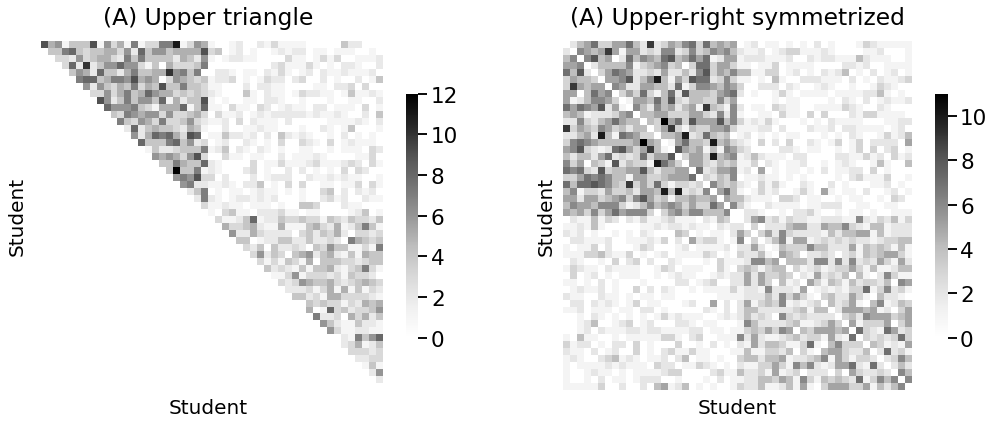
\includegraphics[width=\linewidth]{representations/ch4/Images/triusym.png}
    \caption[Symmetrization through discarding a triangle]{The matrices \texttt{A\_activity\_uppertri} and \texttt{A\_activity\_triu\_symmetrized} showing the \textbf{(A)} upper triangle, \textbf{(B)} and upper-right symmetrized adjacency matrices.}
    \label{fig:ch4:triusym}
\end{figure}
Likewise, if the network only had the lower triangle stored, you could do the same thing but with\texttt{method="tril"} to retain the lower triangle of the matrix.

\paragraph{Taking a function of the two values}

There are many other ways you use a function of $a_{ij}$ and $a_{ji}$ to get a symmetric matrix (and an undirected network). One is to just average. That is, you can let the matrix $A'$ be the matrix with entries $a'_{ij} = \frac{a_{ij} + a_{ji}}{2}$ for all $i$ and $j$. In matrix form, this operation looks like this:

\begin{align*}
    A' &= \frac{1}{2} (A + A^\top) \\
    &= \frac{1}{2}\left(\begin{bmatrix}
        a_{11} & ... & a_{1n} \\
        \vdots & \ddots & \vdots \\
        a_{n1} & ... & a_{nn}
    \end{bmatrix} + \begin{bmatrix}
        a_{11} & ... & a_{n1} \\
        \vdots & \ddots & \vdots \\
        a_{1n} & ... & a_{nn}
    \end{bmatrix}\right)\\
    &= \begin{bmatrix}
        \frac{1}{2}(a_{11} + a_{11}) & ... & \frac{1}{2}(a_{1n} + a_{n1}) \\
        \vdots & \ddots & \vdots \\
        \frac{1}{2} (a_{n1} + a_{1n}) & ... & \frac{1}{2}(a_{nn} + a_{nn})
    \end{bmatrix} \\
    &= \begin{bmatrix}
        a_{11} & ... & \frac{1}{2}(a_{1n} + a_{n1}) \\
        \vdots & \ddots & \vdots \\
        \frac{1}{2} (a_{n1} + a_{1n}) & ... & a_{nn}
    \end{bmatrix}
\end{align*}
As you can see, for all of the entries, $a'_{ij} = \frac{1}{2} (a_{ij} + a_{ji})$, and also $a_{ji}' = \frac{1}{2}(a_{ji} + a_{ij})$. These quantities are the same, so $a_{ij}' = a_{ji}'$, and $A'$ is symmetric. As the adjacency matrix is symmetric, the network that $A'$ represents is undirected.

Remember that the asymmetry in the friendship network means student $i$ might perceive their friendship with student $j$ as being stronger or weaker than student $j$ perceived about student $i$. What you did here was instead of just arbitrarily throwing one of those values away, you said that their friendship might be better indicated by averaging the two values. This produced for us a single friendship strength $a_{ij}'$ where $a_{ij}' = a_{ji}'$.

You can implement this in graspologic as follows:
\begin{lstlisting}[style=python]
# symmetrize with averaging
A_friend_avg_sym = symmetrize(A_friend, method="avg")
\end{lstlisting}
We'd encourage you to plot the outcome and convince yourself that it is, in fact, symmetric using the \texttt{is\_symmetric()} function you learned about in the last section.

We'll will use the friendship network symmetrized by averaging (\texttt{A\_friend\_avg\_sym}) in several of the below examples, which we will call the ``undirected friendship network''.

\subsubsection{Diagonal augmentation}
\label{sec:ch4:regularization:diag_aug}

In your future works with network machine learning, you will come across numerous techniques which operate on adjacency matrices which are \emph{positive semi-definite}. This word doesn't need to mean a whole lot to you conceptually, but it has a big implication when you try to use algorithms on many of your networks. Remember that when you have a loopless network, a common practice in network science is to set the diagonal to zero. What this does is it leads to your adjacency matrices being \emph{indefinite} (which means, \emph{not} positive semi-definite). For our purposes, this means that many network machine learning techniques simply cannot operate on these adjacency matrices. However, as we mentioned before, these entries are not actually zero, but simply \emph{do not exist} and you just didn't have a better way to represent them. Or do you?

\emph{Diagonal augmentation} is a procedure for imputing the diagonals of adjacency matrices for loopless networks. This gives us "placeholder" values that do not cause this issue of indefiniteness, and allow your network machine learning techniques to still work. Remember that for a simple network, the adjacency matrix will look like this:
\begin{align*}
    A &= \begin{bmatrix}
        0 & a_{12} & ... & a_{1n} \\
        a_{21}& \ddots & & \vdots \\
        \vdots & & \ddots & a_{n-1, n} \\
        a_{n1} &...& a_{n, n-1} & 0
    \end{bmatrix}
\end{align*}

What you do is impute the diagonal entries using the \emph{fraction of possible edges which exist} for each node. This quantity is simply the node degree $d_i$ (the number of edges which exist for node $i$) divided by the number of possible edges node $i$ could have (which would be node $i$ connected to each of the other $n-1$ nodes). Remembering that the degree matrix $D$ is the matrix whose diagonal entries are the degrees of each node, the diagonal-augmented adjacency matrix is given by:
\begin{align*}
    A' &= A + \frac{1}{n-1}D = \begin{bmatrix}
        \frac{d_1}{n-1} & a_{12} & ... & a_{1n} \\
        a_{21}& \ddots & & \vdots \\
        \vdots & & \ddots & a_{n-1, n} \\
        a_{n1} &...& a_{n, n-1} & \frac{d_n}{n-1}
    \end{bmatrix}
\end{align*}
When the matrices are directed or weighted, the computation is a little different, but fortunately \texttt{graspologic} will handle this for us. Let's see how you would apply this to the directed friendship network:
\begin{lstlisting}[style=python]
from graspologic.utils import augment_diagonal

A_friend_aug = augment_diagonal(A_friend)
\end{lstlisting}
We will rotate back to the problem of positive semi-definiteness in Section \ref{sec:ch5:psd_block} as it relates to statistical models for networks, and will pivot back again in Section \ref{sec:ch6:spectral} for what it means with regard to adjacency matrices.

\subsection{Regularizing the edges of weighted networks}

As you are probably aware, in all of machine learning, you are always concerned with the \emph{bias/variance tradeoff}. The \textit{bias/variance tradeoff} is an unfortunate side-effect that concerns how well a learning technique will generalize to new datasets \cite{Hastie2009}.
\begin{enumerate}
    \item \textit{Bias} is an error from erroneous assumptions you make about the system that you are learning about. For instance, if you have a friendship network, you might make simplifying assumptions, such as an assumption that two athletes frorm different sports have an equally likely chance of being friends with a member of the band. This might be flat out false, as band members might be selectively better friends with athletes depending on which sports they play.
    \item On the other hand, the \textit{variance} is the degree to which the an estimate of a task will change when given new data. An assumption that if a player is a football player he has a higher chance of being friends with a band member might make sense given that the band performs at football games. 
\end{enumerate}

The "trade-off" is that these two factors tend to be somewhat at odds, in that raising the bias tends to lower the variance, and vice-versa:
\begin{enumerate}
    \item \textit{High bias, but low variance}: Whereas a lower variance model might be better suited to the situation where the data you expect to see is noisy, it might not as faithfully represent the underlying dynamics you think the network possesses. A low variance model might ignore that athletes might have a different chance of being friends with a band member based on their sport all together. This means that while you won't get the student relationships \emph{correct}, you might still be able to get a reasonable estimate that you think is not due to overfitting. In this case, you've smoothed away \emph{signal} from the data at the expense of avoiding \emph{noise}.
    \item \textit{Low bias, but high variance}: Whereas a low bias model might more faithfully model true relationships in your training data, it might fit your training data a little \emph{too} well. Fitting the training data too well is a problem known as \textit{overfitting}. If you only had three football team members and tried to assume that football players were better friends with band members, you might not be able to well approximate this relationship because of how few individuals you have who reflect this situation. 
\end{enumerate}

Here, we show several strategies to reduce the variance (but, add bias) due to edge weight noise in network machine learning.

\subsubsection{Sparsification of the network}

The procedure of \textit{sparsification} is one in which we take a network, and we remove edges from it, which is described by \cite{Spielman2008Aug} and \cite{Batson2013Aug}. Remember that removing edges, in terms of the adjacency matrix, is analogous to setting the corresponding adjacencies to zero. A matrix with many entries of zero is called a \emph{sparse} matrix. So, the reason we call the removal of the edges from a network \emph{sparsification} is that we are producing a network with a \emph{sparse} adjacency matrix.

\emph{Sparsification} is a general class of edge regularization techniques, and includes many flavors. Here, we discuss a few of them. In network sparsification, we will often pick some property of the network (such as, a particular edge weight) and remove edges in an attempt to preserve something about this particular property.

A useful tool to study for how, exactly, you might want to go about sparsifying the network is called the \emph{edge-weight distribution} of your network sample. The edge-weight distribution of the network sample are the particular values that the edge weights of the network take. The most common way to visualize the edge-weight distribution is an edge-weight histogram. This is very similar to the node-degree histogram you worked with above, but instead of node degrees, you look at the edge-weights. Let's take a look at the friendship network, and then take a look at its edge-weight distribution. Remember that the friendship network is \emph{undirected}, so we need to remove its diagonal elements \emph{before} we visualize the edge-weight distribution. We'll also remove edges with zero-weights for visualization purposes:

\begin{lstlisting}[style=python]
def discard_diagonal(A):
    """
    A function that discards the diagonal of a matrix,
    and returns its non-diagonal edge-weights.
    """
    # create a mask that is True for the non-diagonal edges
    non_diag_idx = np.where(~np.eye(A.shape[0], dtype=bool))
    return A[non_diag_idx].flatten()

friend_nondiag_ew = discard_diagonal(A_friend)
# get the non-zero, non-diagonal edge weights
friend_nondiag_nz_ew = friend_nondiag_ew[friend_nondiag_ew > 0]

# plot the histogram, as above
histplot(friend_nondiag_nz_ew, bins=20, binrange=(0, 1))
\end{lstlisting}
We show this plot in Figure \ref{fig:ch4:truncate}(C).

\begin{figure}[h]
    \centering
    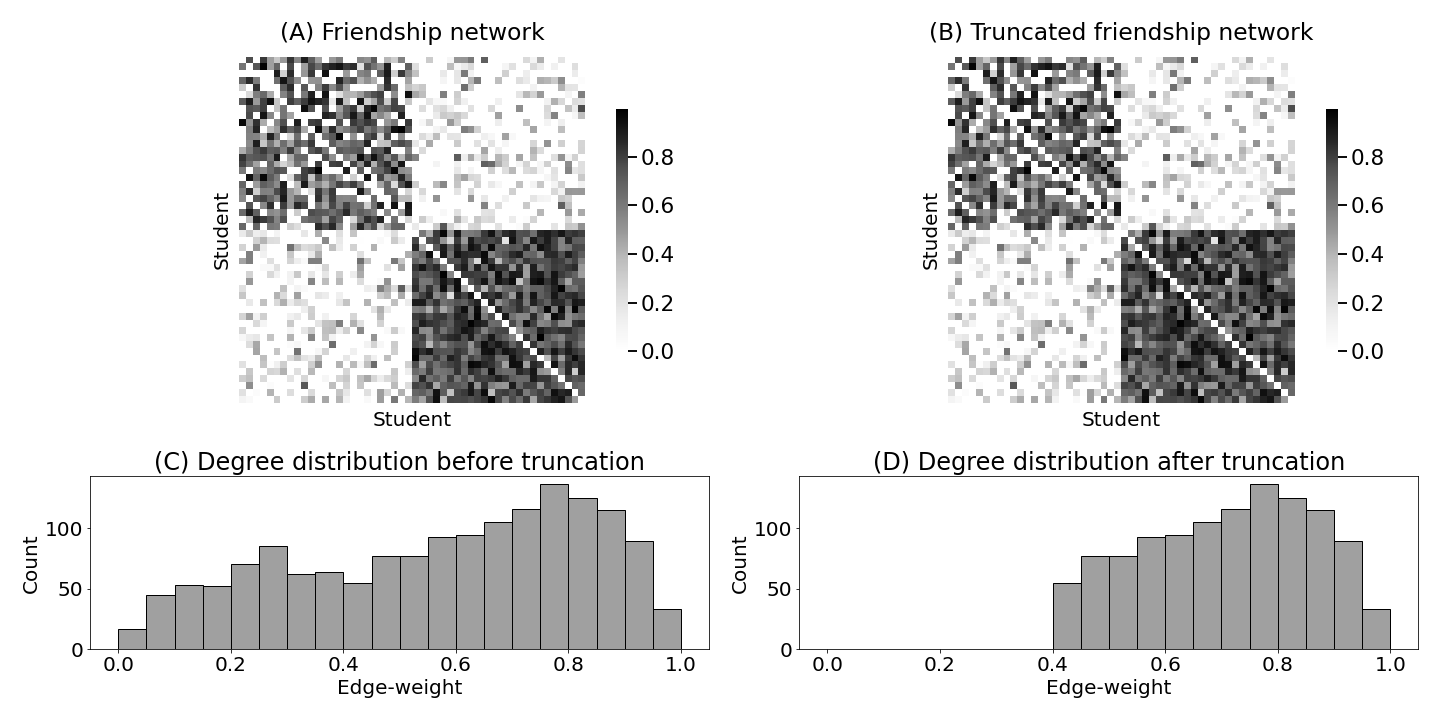
\includegraphics[width=\linewidth]{representations/ch4/Images/truncate.png}
    \caption[Truncation]{\textbf{(A)} The adjacency matrix before truncation. \textbf{(B)} The adjacency matrix after truncation. \textbf{(C)} The non-zero, non-diagonal edge weights before truncation. \textbf{(D)} The non-zero, non-diagonal edge weights after truncation.}
    \label{fig:ch4:truncate}
\end{figure}

\paragraph{Truncation removes the smallest edges}

The simplest way to reduce the variance due to edge weight noise is called \emph{edge truncation}. \textit{Edge truncation} is a process by which you choose some threshold value $\tau$, and remove all of the weights which are smaller than $\tau$ but retain the weights that are bigger than $\tau$. For edges that are equal to $\tau$, what you'll want to do depends on the strategy you are employing. We'll arbitrarily set nodes $\leq \tau$ to zero in our case, but you might use $\geq \tau$ in your uses.

So, how is $\tau$ typically chosen? There are a few ways, but it's usually one of the below two:
\begin{enumerate}
    \item Choose $\tau$ arbitrarily: after looking at your network and doing some preliminary visualizations, you might determine that your edge weights tend to be ``multi-modal''. This means that when you look at the edge-weight distribution, you see multiple "clusters" of edge weight bins which are larger, or smaller. For a lot of networks, these small edges might be very noise induced; that is, the small edges might just spuriously be close to, but {not quite}, zero, due to errors in your measuring process. When the edge weights are really tiny, you might think that these noisy edges are better off just not existing.
    \item Choose $\tau$ based on a particular quantile: A \textit{quantile} is a percentile divided by $100$. In this strategy, you identify a target quantile of the edge-weight distribution. What this means is that you are selecting the lowest {fraction} of the edge-weights (where that fraction is the quantile that you choose) and setting these edges to $0$, and selecting the remaining edges are left unchanged. If you select a quantile of $0.5$, this means that you take the smallest $50\%$ of edges and set them to zero, and the largest $50\%$ of edges and retain their initial value. There are three potential pitfalls to quantiling, which we elaborate on below.
\end{enumerate}
This is called \emph{truncation} because you are taking the edge-weight distribution, and \emph{truncating} (cutting it off) below the value $\tau$.

With respect to what to do with edges that are equal to $\tau$, when you choose a threshold arbitrarily, you can do whatever you want with them, as long as you are consistent if you have multiple networks you are truncating. What we mean by this is that you can select to remove edges less than or equal to this threshold, or retain edge weights greater than or equal to the threshold. When you truncate on the basis of a quantile, however, this is not quite the case. You will want to remove all the edges below $\tau$, and truncate away the remaining edges equal to $\tau$ at random until you have truncated the desired fraction of edges in total.

Let's see how this works in practice. In the edge-weight histogram, in Figure \ref{fig:ch4:truncate} you can notice two "peaks" to the non-zero edge-weights.

If you think that the smaller peak edge-weights are spurious/noise, you might want to threshold somewhere in between the smaller and the larger peaks, like near $0.4$, which is highlighted in \ref{fig:ch4:truncate}(C). 

\begin{lstlisting}[style=python]
def truncate_network(A, threshold):
    A_cp = np.copy(A)
    A_cp[A_cp <= threshold] = 0
    return A_cp

tau = 0.4
A_friend_trunc = truncate_network(A_friend, threshold=tau)
\end{lstlisting}
The next thing to look at is the adjacency matrix, before and after truncation. We show these plots in Figure \ref{fig:ch4:truncate}(A) and \ref{fig:ch4:truncate}(B). Notice that the smallest weight edges in the network (in this case, the ones with edge weights $\leq 0.4$) have been replaced with zeros. As you can see, a lot of the edges in the upper right and upper left, which were previously small, are now \emph{zero}. This is reflected in the edge-weight distribution:

\begin{lstlisting}[style=python]
friend_trunc_nondiag_ew = discard_diagonal(A_friend_trunc)
# get the non-zero, non-diagonal edge weights
friend_trunc_nondiag_nz_ew = friend_trunc_nondiag_ew[friend_trunc_nondiag_ew > 0]
histplot(friend_trunc_nondiag_nz_ew, bins=20, binrange=(0, 1))
\end{lstlisting}
which is shown in Figure \ref{fig:ch4:truncate}(D). As you can see, all of the edges with weights less than $\tau = 0.4$ have been truncated away.

A slight caveat to this procedure we learned about above for truncation is that, if you use the quantile approach and the network is undirected, you need to exclude one triangle of the network to obtain the appropriate quantile. This is because when $a_{ij} = a_{ji}$, you would otherwise count an edge twice if you just used the adjacency matrix to obtain quantiles. We'll see this more in the example on thresholding below.


\paragraph{Thresholding converts weighted networks to unweighted networks}
\label{sec:ch4:regularization:thresholding}

Closely related to truncation is the process of \emph{thresholding}. Like truncation, you begin with a threshold $\tau$, which is usually chosen arbitrarily or based on a quantile, like for truncation. However, there is one key difference: when you threshold a network, you set the edges below $\tau$ to zero, and the edges greater than $\tau$ to \emph{one}. This has the effect of taking a weighted network, and effectively transforming it into an undirected network. 

We will show how to use the quantile approach to thresholding, with the activity/hobby network. You will threshold by choosing $\tau$ such that $\tau$ is the value which is the $0.3$ quantile, or the $30$ percentile, of the edge-weight distribution. Remember as you learned in the preceding section, that if the network itself is loopless, the diagonal entries simply \emph{do not exist}; $0$ is simply a commonly used placeholder. For this reason, when you compute quantiles of edge-weights, you need to \emph{exclude the diagonal} if the network is loopless. 

\begin{floatingbox}[h]\caption{Why is thresholding with a quantile desirable?}\label{box:ch4:desirable}
Remember that in Section \ref{sec:ch4:prop-net:density}, we defined the network density for a simple network as:

\begin{align*}
    density(A) &= \frac{\sum_{j > i}a_{ij}}{\binom{n}{2}}.
\end{align*}

If you threshold this network at a quantile of $q$, this means you will, ideally, set $1 - q$ fraction of the edges to $1$, and a $q$ fraction of the edges to zero.

If we are able to do this perfectly, then $\sum_{j > i}a_{ij} = (1 - q)\binom n 2$.

Therefore:
\begin{align*}
    density(A) &= \frac{(1 - q)\binom n 2}{\binom n 2} = 1 - q
\end{align*}

So when you threshold the network at a quantile $q$, and you are {actually} able to set a $q$ fraction of the edges to zero and a $1 - q$ fraction of the edges to one, you end with a network of density equal to $1 - q$. We will see a for conditions as to when this will, and will not, occur later.
\end{floatingbox}

Further, since this network is undirected, you also need to restrict your attention to one triangle of the corresponding adjacency matrix. We choose the upper-right triangle arbitrarily, as the adjacency matrix's symmetry means the upper-right triangle and lower-right triangle have identical edge-weight distributions. We can do this using \texttt{numpy}. This network is loopless and undirected, so we will want to exclude both the diagonal {and} only perform our analysis on a single triangle of the matrix:
\begin{lstlisting}[style=python]
# find the indices which are in the upper triangle and not in the diagonal
upper_tri_non_diag_idx = np.where(np.triu(np.ones(A_activity.shape), k=1).astype(bool))
q = 0.3  # desired quantile is 0.5, or 50 percentile
histplot(A_activity[upper_tri_non_diag_idx].flatten())
tau = np.quantile(A_activity[upper_tri_non_diag_idx], q=q)
\end{lstlisting}

So, let's see what happens when we just compute $\tau$ using the $q$ quantile of the non-diagonal, upper triangular entries of $A$, and then threshold $A$ using $\tau$. To do this, we'll just check the number of edges greater than $\tau$, and the number less than or equal to $\tau$. Since we used $q = 0.5$ as our desired quantile, we should anticipate that these numbers should be very close to equal:

\begin{lstlisting}[style=python]
n_lteq_tau = np.sum(A_activity[upper_tri_non_diag_idx] <= tau)
n_gt_tau = np.sum(A_activity[upper_tri_non_diag_idx] > tau)
print("Number of edges less than or equal to tau: {}".format(n_lteq_tau))
print("Number of edges greater than to tau: {}".format(n_gt_tau))
\end{lstlisting}
While the specific results you obtain will depend on your specific computer since we used random simulation data here, you're going to get numbers that are not even close to equal (the number of edges $\leq \tau$ should be about 50\% larger than the number of edges $> \tau$). So what happened?

\paragraph{The duplicate value pitfall}

Let's imagine an array that was \texttt{[1,2,3,4]} and \texttt{[1,2,2,4]}, and we chose the $0.5$ quantile, the first array would give a $0.5$ quantile of \texttt{2.5}. If we thresholded with this value, we would get \texttt{[0,0,1,1]}, and the number of elements retained after thresholding would be $50\%$ ones and $50\%$ zeros, like we expected. On the other hand, the $0.5$ quantile of the second array is \texttt{2}, and if we used the thresholding approach above we would get \texttt{[0,0,0,1]}, which has $75\%$ of the values taking $0$ and $25\%$ of the values taking one. 

This means that if you pass in a quantile $q$ and you expect that $q$ fraction of the points will have a value of $0$ after truncation/thresholding, you are going to need to be very careful with your data to handle points that are \emph{equal} to your quantile. To do this, one way is to assign edges less than $\tau$ to zero, and the edges greater than $\tau$ to one. Then, for edges equal to $\tau$, you can to randomly assign them to a zero or one, until you obtain the desired quantiling threshold. This can be done with the pseudocode in Algorithm \ref{alg:ch4:thresholding}. You could write a similar utility for truncating at a quantile.

\begin{algorithm}[h]
    \SetAlgoLined
    \caption{Thresholding an adjcency matrix with random tiebreaking.}
    \label{alg:ch4:thresholding}
    \KwData{$A$: an adjacency matrix \newline $q$: a quantile between $0$ and $1$}
    \KwResult{an adjacency matrix thresholded at the $q$ quantile.}
    Let $d$ be the minimum non-zero difference between any two elements of $A$.
    
    \For{$i$ in $1$ : $n$}{
        \For{$j$ in $1$ : $n$}{
            Let $\epsilon_{ij}$ be a random number between $0$ and $d$.
        }
    }

    \If{$A$ is symmetric}{
        $\epsilon = \frac{\epsilon + \epsilon^\top}{2}$
    }

    Compute the augmented adjacency matrix, $A' = A + \frac{\epsilon}{10}$.

    Compute the appropriate threshold $\tau$ using $A'$.

    Threshold $A'$ by setting elements where $a_{ij}' > \tau$ to one, and $a_{ij}' < \tau$ to zero.
\end{algorithm}

Basically, what this algorithm does is it adds a very small amount of noise to the matrix $A$ that you are thresholding. Note that we take care to ensure that if $A$ is symmetric and the network is undirected, that we add the \emph{same} amount of noise to both entries $a_{ij}$ and $a_{ji}$ by \emph{symmetrizing} this ``noise matrix'' $\epsilon$. This noise is small enough that it is an order of magnitude (a factor of $10$) smaller than the smallest appreciable difference in any two non-zero elements of $A$. 

After we add this matrix to $A$, there is a probability of \emph{zero} that any two elements of $A$ will have the same value. Further, since we added noise that was an order of magnitude smaller than any non-zero differences of elements of $A$, it is impossible for an item that was originally greater than a quantile to now be less than the desired quantile, and vice-versa. This strategy is called a random tiebreaking, since we broke ties that occur at exactly the $q$ quantile randomly.

This can be implemented in python as follows:

\begin{lstlisting}[style=python]
from numpy import copy

def min_difference(arr):
    b = np.diff(np.sort(arr))
    return b[b>0].min()

def quantile_threshold_network(A, directed=False, loops=False, q=0.5):
    # a function to threshold a network on the basis of the
    # quantile
    A_cp = np.copy(A)
    n = A.shape[0]
    E = np.random.uniform(low=0, high=min_difference(A)/10, size=(n, n))
    if not directed:
        # make E symmetric
        E = (E + E.transpose())/2
    mask = np.ones((n, n))
    if not loops:
        # remove diagonal from E
        E = E - np.diag(np.diag(E))
        # exclude diagonal from the mask
        mask = mask - np.diag(np.diag(mask))
    Ap = A_cp + E
    tau = np.quantile(Ap[np.where(mask)].flatten(), q=q)
    A_cp[Ap <= tau] = 0; A_cp[Ap > tau] = 1
    return A_cp

A_activity_thresholded03 = quantile_threshold_network(A_activity, q=0.3)
A_activity_thresholded07 = quantile_threshold_network(A_activity, q=0.7)
\end{lstlisting}
We visualize these two thresholded adjacency matrices along with the unweighted adjacency matrix in Figure \ref{fig:ch4:threshold_res}.

\begin{figure}[h]
    \centering
    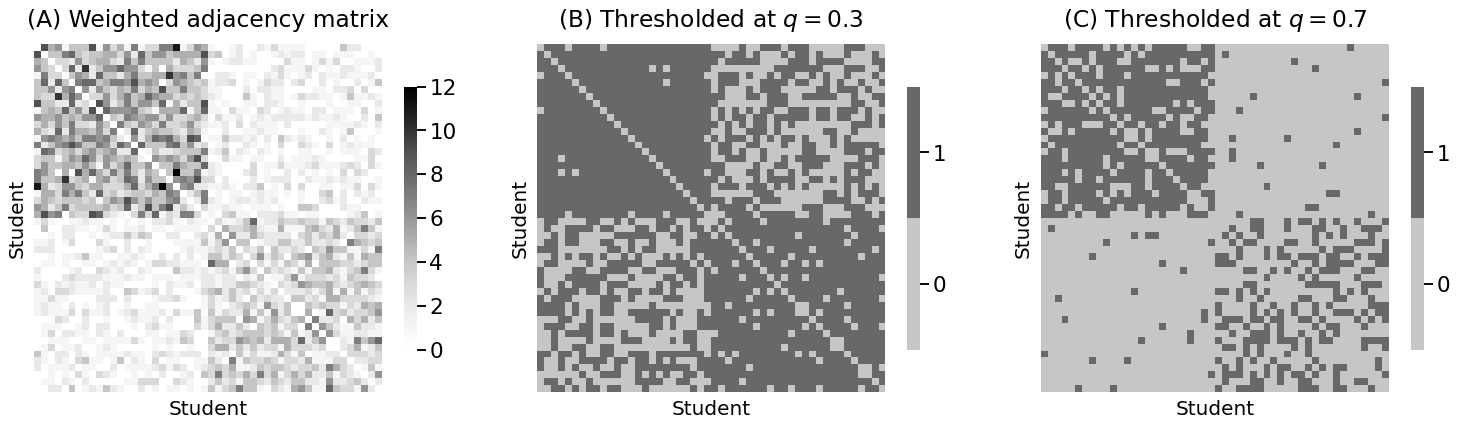
\includegraphics[width=\linewidth]{representations/ch4/Images/threshold_res.png}
    \caption[Thresholding]{\textbf{(A)} the weighted adjacency matrix of the activity/hobby network. \textbf{(B)} the weighted adjacency matrix of the activity/hobby network after thresholding at $0.3$. \textbf{(C)} the weighted adjacency matrix of the activity/hobby network after thresholding at $0.7$.}
    \label{fig:ch4:threshold_res}
\end{figure}

Great job. Now, let's just confirm that we didn't run into the duplicate value pitfall. We'll do this by writing a utility which computes the network density from an adjacency matrix for a simple network:

\begin{lstlisting}[style=python]
from graspologic.utils import is_unweighted, is_loopless, is_symmetric

def simple_network_dens(X):
    # make sure the network is simple
    if (not is_unweighted(X)) or (not is_loopless(X)) or (not is_symmetric(X)):
        raise TypeError("Network is not simple!")
    # count the non-zero entries in the upper-right triangle
    # for a simple network X
    nnz = np.triu(X, k=1).sum()
    # number of nodes
    n = X.shape[0]
    # number of possible edges is 1/2*n*(n-1)
    poss_edges = 0.5*n*(n-1)
    return nnz/poss_edges

print("Network Density: {:.3f}".format(simple_network_dens(A_activity_thresholded03)))
# Network Density: 0.700
\end{lstlisting}

So our solution achieved the desired network density.

We call this pitfall the \emph{duplicate value pitfall} because you can \emph{only} run into it if your adjacency matrix has the same value duplicated.

\paragraph{The ``underly ambitious'' pitfall}

The next pitfall of using a quantile $q$ is actually a special case of the duplicate value pitfall listed above: you might choose an underly ambitious quantile to truncate/threshold with. By underly ambitious, what we mean is that the adjacency matrix doesn't even have a $1 - q$ fraction of non-zero edges. When you threshold $A$ with a quantile of $q$, you can spot this pitfall fairly easily by simply checking the fraction of $0$-weight edges ahead of time.

For an example, let's consider a network where $50\%$ of the possible edges are zero (the network density is $0.5$, and the other $50\%$ are one. If you were to choose a quantile of $0.3$, quantiling will still only give you a network density of $0.5$, and not $0.7$ like you might have expected from Remark \ref{box:ch4:desirable}.

Unfortunately, there's no quick fix like there was for the non-continuous pitfall; if you run into the underly ambitious pitfall and tried to use the randomization procedure, the ``solution'' would end up setting edges with a value of zero in the adjacency matrix to one, which doesn't make much sense. To avoid this pitfall, you need to analyze your densities ahead of time if you want to use quantiling, and ensure that the quantile you choose is not underly ambitious. 

If you had a collection of networks that you wanted to threshold or truncate \emph{en masse} using a quantile $q$, you could do this by plotting a histogram of your network densities, and ensuring that $1 - q$ is less than all of the network densities in your collection.

\begin{floatingbox}[h]\caption{With all these pitfalls, why would we quantile?}
As we mentioned in Section \ref{sec:ch4:net-rep:featurelims}, many network summary statistics that you might be interested in could be heavily correlated with the network density. For this reason, if you want to analyze a collection of networks using summary statistics, it might make sense to analyze a collection of networks with the same network density. This is because in some sense, analyzing the networks with a similar network density will ``decouple'' this correlation with the network density, since the network density will no longer be changing across the networks.
\end{floatingbox}

\paragraph{When can we ignore these pitfalls entirely?}

As you might be able to gather from the above, if our network fulfills two properties, we are guaranteed that we won't run into the quantiling pitfalls. First, if the network is \textit{dense} (a network where all possible entries $a_{ij}$ are non-zero, with arbitrarily small or large edge-weights), we cannot possibly run into the underly ambitious pitfall, since that pitfall will only arise when there are zero-weight edges in the adjacency matrix. Second, if the adjacency matrix does not have any duplicate values, we cannot run into the duplicate value pitfall either, because we cannot have ties at the desired quantile if there are no duplicated values in the edge weights. 

As we have repeated many times in this section, when considering when a network might run into these pitfalls using the adjacency matrix, be sure to only consider appropriate entries of the adjacaency matrix. This means restricting your analysis to the upper triangle or the lower triangle if the netework is undirected, and removing the diagonal if the network is loopless. 

\subsubsection{Edge-weight global rescaling}

With weighted networks, it is often the case that you might want to reshape the distributions of edge-weights in your networks to highlight particular properties. Notice that the edge-weights for your friendship network takes values between $0$ and $1$, but your activity network takes values between $0$ and almost $15$. How can you possibly compare between these two networks where the edge-weights take such different ranges of values? You turn to standardization, which allows us to place values from different networks on the same scale. 

\paragraph{$z$-scoring standardizes edge weights using the normal distribution}

The first approach to edge-weight standardization is known commonly as $z$-scoring. Suppose that $A$ is the adjacency matrix, with entries $a_{ij}$. With a $z$-score, you will rescale the weights of the adjacency matrix, such that the new edge-weights (called $z$-scores) are approximately normally distributed. The reason this can be useful is that the normal distribution is pretty ubiquitous across many branches of science, and therefore, a $z$-score is relatively easy to communicate with other scientists. Further, many things that exist in nature can be well-approximated by a normal distribution, so it seems like a reasonable place to start to use a $z$-score for edge-weights, too! The $z$-score is defined as follows. You will construct the $z$-scored adjacency matrix $Z$, whose entries $z_{ij}$ are the corresponding $z$-scores of the adjacency matrix's entries $a_{ij}$. For a weighted, loopless network, you use an estimate of the \emph{mean}, $\hat \mu$, and the \emph{unbiased} estimate of the \emph{variance}, $\hat \sigma^2$, which can be computed as follows:
\begin{align*}
    \hat\mu &= \frac{1}{n(n-1)}\sum_{i \neq j}a_{ij},\\
    \hat\sigma^2 &= \frac{1}{n(n - 1) - 1}\sum_{i \neq j} (a_{ij} - \hat\mu)^2.
\end{align*}
The $z$-score for the $(i,j)$ entry is simply the quantity:
\begin{align*}
    z_{ij} &= \frac{a_{ij} - \hat\mu}{\hat\sigma}
\end{align*}
Since your network is loopless, notice that these sums are for all \emph{non-diagonal} entries where $i \neq j$. If the network were not loopless, you would include diagonal entries in the calculation, and instead would sum over all possible combinations of $i$ and $j$. the interpretation of the $z$-score $z_{ij}$ is the \emph{number of stadard deviations} that the entry $a_{ij}$ is from the mean, $\hat \mu$.

We will demonstrate on the directed friendship network. You can implement $z$-scoring as follows:

\begin{lstlisting}[style=python]
from scipy.stats import zscore

def z_score_loopless(X, undirected=False):
    if not is_loopless(X):
        raise TypeError("The network has loops!")
    if is_symmetric(X):
        raise TypeError("The network is undirected!")
    # the entries of the adjacency matrix that are not on the diagonal
    non_diag_idx = np.where(~np.eye(X.shape[0], dtype=bool))
    Z = np.zeros(X.shape)
    Z[non_diag_idx] = zscore(X[non_diag_idx])
    return Z

ZA_friend = z_score_loopless(A_friend)
\end{lstlisting}

The theory for when, and why, to use $z$-scoring for network machine learning tends to go something like this: many things tend to be normally distributed with the same mean and variance, so perhaps that is a reasonable expectation for your network, too. Unfortunately, we find this often to \emph{not} be the case. In fact, we often find that the specific distribution of edge weights itself often might be lamost infeasible to identify in a population of networks, and therefore \emph{almost} irrelevant all-together. To this end, we turn to instead \emph{ranking} the edges.

Note that in the above code snippet, we throw an error if the network is undirected (and the adjacency matrix is symmetric): remember that you want to be careful to restrict your analysis to the upper triangle if the network is undirected and loopless. This won't really change the estimate of the mean, but the variance will be slightly different. The sums would be over $j > i$, and the normalizing factors would be $\binom n 2$ instead of $n(n - 1)$.

\paragraph{Ranking edges preserves ordinal relationships}

The idea behind ranking is as follows. You don't really know much useful information as to how the distribution of edge weights varies between a given pair of networks. For this reason, you want to virtually eliminate the impact of that distribution \emph{almost} entirely. However, you know that if one edge-weight is larger than another edge-weight, that you do in fact trust that relationship. What this means is that you want something which preserves \emph{ordinal} relationships in your edge-weights, but ignores other properties of the edge-weights. An ordinal relationship just means that you have a natural ordering to the edge-weights. This means that you can identify a largest edge-weight, a smallest edge-weight, and every position in between. When we want to preserve ordinal relationships in your network, we do something called \emph{passing the non-zero edge-weights to ranks}. We will often use the abbreviation\texttt{ptr} to define this function because it is so useful for weighted networks. We pass non-zero edge-weights to ranks as in Algorithm \ref{alg:ch4:ptr}.

\begin{algorithm}[h]
    \SetAlgoLined
\caption{Passing an adjacency matrix to ranks}
\label{alg:ch4:ptr}
    \KwData{$A$ is an adjacency matrix.}
    \KwResult{The adjacency matrix, after passing to ranks.}
    Identify all of the non-zero entries of the adjacency matrix $A$.

    Let $n_{nz}$ be the number of non-zero entries of the adjacency matrix $A$.

    Rank all of the non-zero edges in the adjacency matrix $A$, where for a non-zero entry $a_{ij}$, $rank(a_{ij}) = 1$ if $a_{ij}$ is the smallest non-zero edge-weight, and $rank(a_{ij}) = n_{nz}$ if $a_{ij}$ is the largest edge-weight. Ties are settled by using the average rank of the tied entries.

    Report the weight of each non-zero entry $(i,j)$ as $r_{ij} = \frac{rank(a_{ij})}{n_{nz} + 1}$, and for eachh zero entry as $r_{ij} = 0$.
\end{algorithm}

Below, we pass-to-ranks the directed friendship network using\texttt{graspologic}:

\begin{lstlisting}[style=python]
from graspologic.utils import pass_to_ranks

RA_friend = pass_to_ranks(A_friend)
\end{lstlisting}

A plot of the adjacency matrices before and after passing to ranks, as well as the edge-weight histograms before and after passing to ranks, is shown in Figure \ref{fig:ch4:ptr}.

\begin{figure}[h]
    \centering
    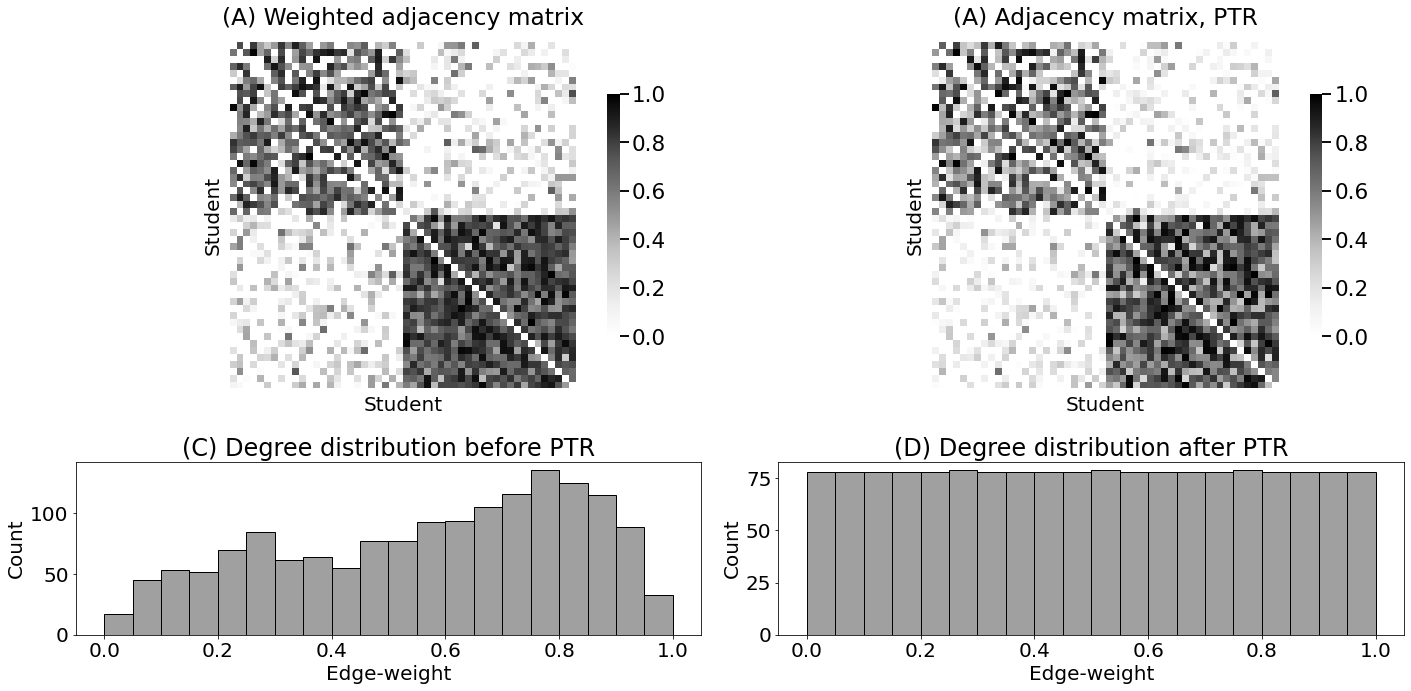
\includegraphics[width=\linewidth]{representations/ch4/Images/ptr.png}
    \caption[Passing to ranks to normalize edge-weights]{\textbf{(A)} the adjacency matrix before passing to ranks for the friendship network. \textbf{(B)} the adjacency matrix after passing to ranks. \textbf{(C)} the edge-weight histogram (including zero-weight edges) before passing to ranks. \textbf{(D)} the edge-weight histogram (including zero-weight edges) after passing to ranks.}
    \label{fig:ch4:ptr}
\end{figure}
The edge-weights for the adjacency matrix $R$ after \texttt{ptr} has the interpretation that each entry $r_{ij}$ which is non-zero is the \emph{quantile} of that entry amongst \emph{the other non-zero entries}. This is unique in that it is completely \emph{distribution-free}, which means that you don't need to assume anything about the distribution of the edge-weights to have an interpretable quantity. On the other hand, the $z$-score had the interpretation of the number of standard deviations from the mean, which is only a sensible quantity to compare if you assume the population of edge-weights are normally distributed.


Another useful quantity related to pass-to-ranks is known as the zero-boosted pass-to-ranks. Zero-boosted pass-to-ranks is conducted as in Algorithm \ref{alg:ch4:ptr_zb}.

\begin{algorithm}[h]
\SetAlgoLined
\caption{Zero-boosted pass to ranks}
    \KwData{$A$ is an adjacency matrix.}
    \KwResult{The adjacency matrix, after passing to ranks.}
    Identify all of the non-zero entries of the adjacency matrix $A$ and the zero-weighted entries of the adjacency matrix $A$.

    Let $n_{nz}$ be the number of non-zero entries of the adjacency matrix $A$, and $n_z$ be the number of zero-weighted entries of the adjacency matrix $A$. Note that $n_{nz} + n_z = n^2$, since $A$ has $n^2$ entries.

    Rank all of the non-zero edges in the adjacency matrix $A$, where for a non-zero entry $a_{ij}$, $rank(a_{ij}) = 1$ if $a_{ij}$ is the smallest non-zero edge-weight, and $rank(a_{ij}) = n_{nz}$ if $a_{ij}$ is the largest edge-weight. Ties are settled by using the average rank of the two entries.

    Report the weight of each non-zero entry $(i,j)$ as $r_{ij}' = \frac{n_z + rank(a_{ij})}{n^2 + 1}$, and for each zero entry as $r_{ij}' = 0$.
\end{algorithm}

The edge-weights for the adjacency matrix $R'$ after zero-boosted\texttt{ptr} have the interpretation that each entry $r_{ij}'$ is the quantile of that entry amongst \emph{all} of the entries. Let's instead use zero-boosted\texttt{ptr} on your network:

\begin{lstlisting}[style=python]
RA_friend_zb = pass_to_ranks(A_friend, method="zero-boost")
\end{lstlisting}
We show the adjacency matrix after zero-boosted \texttt{ptr}, along with the edge-weight histogram (including zero-weight edges), in Figure \ref{fig:ch4:ptr_zb}.

\begin{figure}[h]
    \centering
    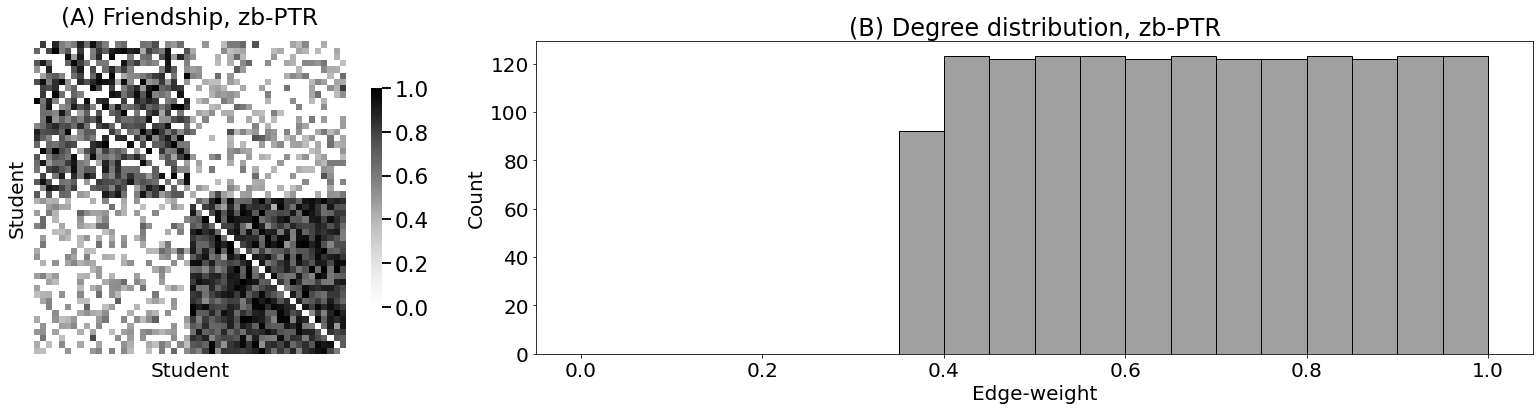
\includegraphics[width=\linewidth]{representations/ch4/Images/ptr_zb.png}
    \caption[Zero-Boosted PTR]{\textbf{(A)} the adjacency matrix, after zero-boosted\texttt{ptr}. \textbf{(B)} the edge-weight histogram, after zero-boosted\texttt{ptr}. Compare this to Figure \ref{fig:ch4:ptr}(B) and \ref{fig:ch4:ptr}(D), respectively.}
    \label{fig:ch4:ptr_zb}
\end{figure}

\paragraph{Thresholding as a decimation of ranking}
As it turns out, the thresholding approach you learned in Section \ref{sec:ch4:regularization:thresholding} can be thought of as a \emph{decimation} of ranking, assuming that the ranking implementation handles ties randomly (the implementation in\texttt{graspologic} does not, as ties are settled by the average rank, but we would encourage you to implement one that \emph{does} as an exercise). For instance, if you picked a threshold of $0.5$, there is some corresponding rank (or value in between two ranks), where all of the elements of the adjacency matrix with a rank lower than a given threshold $\tau_r$ have corresponding weights lower than $\tau$ and all of the elements of the adjacency matrix with a rank higher than a given threshold $\tau_r$ have corresponding weights higher than $\tau$. Then, you can simply threshold the ranked adjacency matrix using $\tau_r$.

\paragraph{Logging reduces magnitudinal differences between edges}
\label{sec:ch4:regularization:logscale}

When we look at the distribution of non-zero edge-weights for the activity/hobby network or the friendship network, we notice a strange pattern, known as a \emph{right-skew}. This is shown in Figure \ref{fig:ch4:log}(A). Informally, a distribution is \emph{right-skewed} if a large fraction of the points take relatively small values, and then a small portion of the points take relatively large values. Notice in this figure, for instance, that most points have an edge weight between $0$ and $2$, but and a small portion of points have an edge-weight between $2$ and $10$. This is called a ``right-skew'' because the histogram ``tails off'' as the values go to the right (increase). 


What if you want to make these large values more similar in relation to the smaller values, but you simultaneously want to preserve properties of the underlying distribution of the edge-weights? Well, you can't use\texttt{ptr`, because `ptr} will throw away all of the information about the edge-weight distribution other than the ordinal relationship between pairs of edges. To interpret what this means, you might think that there is a big difference between sharing no interests compared to three interests in common, but there is not as much of a difference in sharing ten interests compared to thirteen interests in common.

To do this, we instead turn to the logarithm function. The logarithm function $log_{10}(x)$ is defined for positive values $x$ as the value $c_x$ where $x = 10^{c_x}$. In this sense, it is the "number of powers of ten" to obtain the value $x$. The logarithm function is shown in Figure \ref{fig:ch4:log}(B).

\begin{figure}
    \centering
    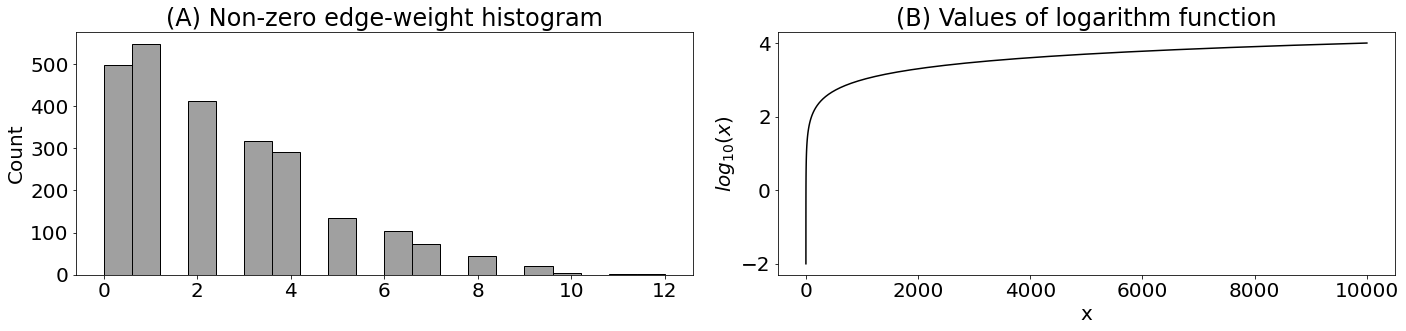
\includegraphics[width=\linewidth]{representations/ch4/Images/log.png}
    \caption[Heavy tailed edge-weights]{\textbf{(A)} The non-zero edge-weight histogram for the activity/hobby network. Notice that the histogram ``tails off'' towards the right. \textbf{(B)} The value for the base-$10$ logarithm function for given values of $x$.}
    \label{fig:ch4:log}
\end{figure}

What is key to noice about this function is that, as $x$ increases, the log of $x$ increases by a \emph{decreasing} amount. Let's imagine you have three values, $x = .001$, $y = .1$, and $z = 10$. A calculator will give you that $log_{10}(x) = -3, log_{10}(y) = -1$, and $log_{10}(z) = 1$. Even though $y$ is only $.099$ units bigger than $x$, its logarithm $log_{10}(y)$ exceeds $log_{10}(x)$ by two units. on the other hand, $z$ is $9.9$ units bigger than $y$, but yet its logarithm $log_{10}(z)$ is still the same two units bigger than $log_{10}(y)$. This is because the logarithm is instead looking at the fact that $z$ is \emph{one} power of ten, $y$ is $-1$ powers of ten, and $z$ is $-3$ powers of ten. The logarithm has \emph{collapsed} the huge size difference between $z$ and the other two values $x$ and $y$ by using exponentiation with \emph{base} ten. 


In this sense, you can also use the logarithm function for your network to reduce the huge size difference between the values in your activity/hobby network. However, we must first add a slight twist: to do this properly and yield an interpretable adjacency matrix, you need to \emph{augment} the entries of the adjacency matrix \emph{if} it contains zeros. This is because the $log_{10}(0)$ is \emph{not defined}. To augment the adjacency matrix, we'll basically ``inflate'' these values by a magnitude that is negligibly small. We show how to implement this in Algorithm \ref{alg:ch4:log_xfm}.

\begin{algorithm}[h]
    \SetAlgoLined
    \caption{Log transforming a network with zero-weight edges.}
    \KwData{$A$ is an adjacency matrix. \newline $b$ the base to log transform with.}
    \KwResult{The adjacency matrix, after log transformation.}

    Identify the entries of $A$ which take a value of zero.

    Identify the smallest entry of $A$ which is not-zero, and call it $a_m$.

    Compute a value $\epsilon$ which is an \emph{order of magnitude} smaller than $a_m$. Since you are taking powers of $b$, a single order of magnitude would give us that $\epsilon = \frac{a_m}{b}$. 

    Take the augmented adjacency matrix $A'$ to be defined with entries $a_{ij}' = a_{ij} + \epsilon$.

    Log transform $A'$ with a base of $b$.
\end{algorithm}

The first process of this procedure is called a \emph{zero augmentation}. We can code up the log transformation as follows:


\begin{lstlisting}[style=python]
def augment_zeros(X, base=10):
    if np.any(X < 0):
        raise TypeError("The logarithm is not defined for negative values!")
    am = np.min(X[np.where(X > 0)])  # the smallest non-zero entry of X
    eps = am/base  # epsilon is one order of magnitude smaller than the smallest non-zero entry
    return X + eps  # augment all entries of X by epsilon
def log_transform(X, base=10):
    """
    A function to log transform an adjacency matrix X, which may
    have zero-weight edges.
    """
    X_aug = augment_zeros(X, base=base)
    return np.log(X_aug)/np.log(base)

A_activity_log = log_transform(A_activity)
\end{lstlisting}

We plot the untransformed and log-transformed activity/hobby network in Figure \ref{fig:ch4:log_xfm}. 

When you plot the augmented and log-transformed data, what you see is that many of the edge-weights you originally might have thought were zero if you only looked at a plot were, in actuality, \emph{not} zero. In this sense, for non-negative weighted networks, log transforming after zero-augmentation is often very useful for visualization to get a sense of the magnitudinal differences that might be present between edges, since you can get a better feel for how different the big weights are from the smaller weights.

\begin{figure}[h]
    \centering
    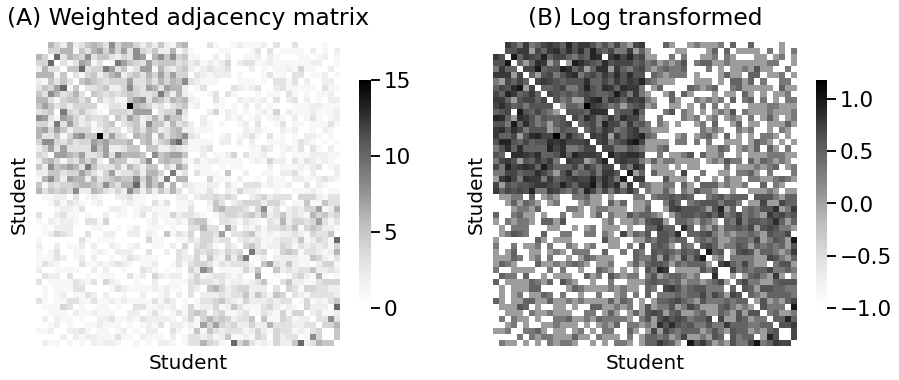
\includegraphics[width=\linewidth]{representations/ch4/Images/log_xfm.png}
    \caption[Log-transforming heavy-tailed edge-weights]{\textbf{(A)} The weighted adjacency matrix for the activity/hobby network. Notice that there are many entries which are very small, and it is hard to discern which entries are zero from the entries that are just tiny. \textbf{(B)} The activity/hobby network, after log transformation. Notice that the edges which are zero are readily apparent in the plot, and we have a better sense of the range of non-zero elements visually as well (they tend to fall between $0$ and $1$, so are different by approximately a power of $10$).}
    \label{fig:ch4:log_xfm}
\end{figure}


\bibliographystyle{vancouver}
\bibliography{references}
\chapter{Why use Statistical Models?}
\label{sec:ch5}

At the foundation of statistical inference is the statistical model. This concept can seem somewhat esoteric, and often times, the word "statistical model", we find, is a bit overused. However, it is extremely important to clarify exactly what a statistical model is, and what it isn't, so we hope to clear up some of those misconceptions here before we jump in. A statistical model is, at its core, {purely theoretical} in nature. Statistical models fit into the network learning pipeline like in Figure \ref{fig:ch5:netmodels}:
\begin{figure}[h]
    \centering
    \includegraphics[width=\linewidth]{representations/ch5/Images/network_modelling.png}
    \caption[Network modelling schematic]{In this chapter, you will learn how to construct sets of assumptions about the network which underlies your network sample.}
    \label{fig:ch5:netmodels}
\end{figure}

The reality is, the network you observe, which you learned how to describe in the previous chapter, is not {typically} the thing you want to learn about. Rather, you want to learn about the {system} which underlies the network you observed. To learn about the dynamics of this system is a three-step process: first, you need to assume some things about the system (this chapter); second, you need to learn representations of the network you see that will be useful to you (the next chapter), and finally, you need to learn how that representation can inform the assumptions you made about the system. This process can be boiled down quite a bit to how flipping a coin works. When you flip a coin, usually you don't know ahead of time whether that coin is going to land on heads or tails. Instead, you think that coin is going to land on heads or tails with some probability (usually, an even chance of landing on heads or tails, or a probability of $0.5$). If you flip the coin once and get heads, you don't think that coin is {only} going to ever land on heads: rather, you think that coin landed on heads because of some amount of random chance. 

And herein, you just assumed a statistical model. You assumed that the outcome of your coin (the random object, here, that you are modelling) was heads or tails with some probability, and when you saw that outcome (the {sample} of the coin flip) you prescribed that outcome to one of the possible outcomes occurring. As you'll see briefly, network modelling is nearly the same, and for simple networks especially, is {almost exactly} the same as flipping coins. Throughout this chapter, you'll learn to think about each edge of the network as a particular coin. Remember that the edges for a simple (and consequently, {unweighted}) network either exist or they don't exist: this is exactly like a coin landing on heads or tails. The key difference is that the edges existing or not existing might happen at probabilities different from $0.5$; there might be a chance of $0.7$ that one edge exists, or $0.4$ that another edge exists. 

When you construct models for networks, what you are going to do is prescribe sets of assumptions for how the coin for each edge behaves: are all of the edges in the network flipping coins with equal probability (do all the edges exist or not exist with the same chance)? Are there some groups of nodes whose edges all have the same probabilities? Are there other ways you can describe the probabilities that other edges exist or do not exist? 

\begin{comment}
We'll learn about the following models, which tend to be some of the more common simple network models for network learning:

\begin{enumerate}
    \item Section \ref{sec:ch5:er} covers the Erd\"os-R\'enyi (ER) random network, which is the simplest model for network data.
    \item Section \ref{sec:ch5:sbm} covers the Stochastic Block Model (SBM), which is a model for network data that conveys community structure.
    \item Section \ref{sec:ch5:rdpg} covers the Random Dot Product Graph (RDPG), which is a model which we will use later to conceptualize techniques to learn representations of network data.
    \item Section \ref{sec:ch5:ier} covers the Inhomogeneous Erd\"os R\'enyi (IER) random network, which is the most complicated independent-edge network model.
    \item Section \ref{sec:ch5:dcsbm} covers the degree-corrected SBM (DCSBM), which is an augmentation of the SBM that allows for some nodes to be more (or less) connected than others.
    \item Section \ref{sec:ch5:psd_block} covers different types of block matrices for SBMs, and when these can be conceptualized using an RDPG.
    \item Section \ref{sec:ch5:siem} covers the structured independent-edge model (SIEM), which will be used later to facilitate testing on groups of edges in the network.
    \item Section \ref{sec:ch5:multi} covers network models for when we have more than one network.
    \item Section \ref{sec:ch5:multicovar} covers the signal subnetwork (SSN) model, a model for when we have network-specific covariates.
\end{enumerate}
\end{comment}

Network modelling can get pretty dicey in probability and statistical theory rather quickly. For this reason, for the main text of the book, we've tried to keep the level of statistical depth required as low as possible, so that you can focus more on the intuition and mathematical relationships and less on the statistical rigor. For the more technical readers, Appendix \ref{app:ch12} provides more in-depth coverage of statistical network models.

\newpage

\section{Erd\"os-R\'enyi Random Networks}
\label{sec:ch5:er}


We will start to learn about random networks with the simplest random network model. Consider a social network, with 50 students. Our network will have 50 nodes, where each node represents a single student in the network. Edges in the social network represent whether or not a pair of students are friends. What is the simplest way you could describe whether two people are friends?

In network machine learning, you get to see an adjacency matrix $A$ whose entries $a_{ij}$ are one if the students $i$ and $j$ are friends on the social networking site, and $0$ if the students $i$ and $j$ are not friends on the social networking site. You have $n$ students in total, so the adjacency matrix $A$ is going to be $n \times n$. 

\begin{floatingbox}[h]\caption{Making the leap to statistical modelling with coin flips}
When you have a coin, before you flip it, the outcome is either heads or tails, with some probability. We'll denote this coin, for which we don't know the outcome (because we haven't flipped it), by the letter $\mathbf x$. 

The best way that we can describe this coin is not by heads and tails, but rather, by {probabilities} that it lands on heads or tails. For a coin, what we'd say is that a sample $x$ (an outcome of a flip of the coin $\mathbf x$) is heads with probability $p$ or tails with probability $1-p$ (the coin can only land on heads or tails, so the probabilities must sum up to $1$). 

When specifying the statistical model, you don't make any assumptions about the probabilities; you just specify that they are probabilities, and leave it at that. For a normal, {fair} coin, $p$ would be $0.5$, but we don't even want to get that specific when we come up with a statistical model for a system.
\end{floatingbox}

Now, let's rotate back to the network. Since our observation $A$ was an $n \times n$ matrix, our random variable $\mathbf A$ is an $n \times n$ random matrix. The elements of $\mathbf A$ will be given by the symbols $\mathbf a_{ij}$, which means that each edge $a_{ij}$ of $A$ is a sample of the random edge $\mathbf a_{ij}$. Just how do you describe this $\mathbf a_{ij}$? 

Remember that our samples $a_{ij}$ are just $0$s and $1$s, which {feels} a lot like flipping a coin, doesn't it? Did the coin land on heads, or did it land on tails? Are the two people $i$ and $j$ friends, or are they not friends? If you had a coin with some probability of landing on heads, you could describe $a_{ij}$ as a sample of this coin flip. You could assume that a value of one is analogous to the coin landing on heads, and value of zero is analogous to the coin landing on tails. Perhaps you could even model the network using the same approach you took before with the coin flip. This is starting to go somewhere, so let's continue with the analogies.


\subsection{The Erd\"os R\'enyi random network is parametrized by the independent-edge probability}

The simplest random network model is called the Erd\"os R\'enyi (ER) model, which was first described by \cite{erdos59a} and \cite{Gilbert1959Dec}. The way you can think of an ER random network is that the edges depend {only} on a probability, $p$, and each edge is totally independent of all other edges. You can think of this example as though a coin flip is performed, where the coin has a probability $p$ of landing on heads, and $1-p$ of landing on tails. For each edge in the network, you conceptually flip the coin, and if it lands on heads (with probability $p$), the edge exists, and if it lands on tails (with probability $1-p$) the edge does not exist. If $\mathbf A$ is a random network which is $ER_n(p)$ with $n$ nodes and probability $p$, we will say that $\mathbf A$ is an $ER_n(p)$ random network.

\begin{floatingbox}[h]\caption{What part of this is the statistical model?}
The statistical model, here, is just the description of the system. {All} of the edges of the underlying random network, $\mathbf A$, have a probability $p$ of existing or not existing. This probability is the same for all edges. The edges are independent, and whether one edge exists does not impact whether any other edges exist. 

Again, the probability is left generic in the statistical model: it is just $p$, which could be $0.5$, $0.7$, $0.4$, really just any probability (a number between $0$ and $1$). It's really as simple as that!
\end{floatingbox}


\subsection{How do you simulate samples of $ER_n(p)$ random networks?}

This approach which you will use to describe random networks is called a {generative model}, which means that you have described an observable network sample $A$ of the random network $\mathbf A$ in terms of the parameters of $\mathbf A$. In the case of the ER random networks, you have described $\mathbf A$ in terms of the probability parameter, $p$. Generative models are convenient in that you can easily adapt them to tell us exactly how to simulate samples of the underlying random network. The procedure in Algorithm \ref{alg:ch5:er} will produce for us a network $A$, which has nodes and edges, where the underlying random network $\mathbf A$ is an $ER_n(p)$ random network.

\begin{algorithm}[h]\caption{Simulating a sample from an $ER_n(p)$ random network}
\label{alg:ch5:er}
\SetAlgoLined
\KwData{$n$ a number of nodes\newline $p$ a probability of an edge existing}
\KwResult{The adjacency matrix of a sample from the random network.}

Obtain a weighted coin which has a probability $p$ of landing on heads, and a probability $1 - p$ of landing on tails. Note this probability $p$ might differ from the "traditional" coin with a probability of landing on heads of approximately $0.5$.

\For{$i$ in $1$:$n$} {
    \For{$j > i$} {
        Flip the coin once. If the coin lands on heads, let $a_{ij} = 1$. If the coin lands on tails, let $a_{ij} = 0$.

        Let $a_{ji} = a_{ij}$.
    }
}

\Return{$A$}
\end{algorithm}

\begin{floatingbox}[h]\caption{Notation and word choice regarding networks and random networks}
When you are deciding on notation that you will use for your work, it is {extremely} easy to get confused very quickly. Within this work, since we are regularly dealing with matrices, vectors, and scalar quantities, we use boldface $\mathbf A$ to denote a network which is random. 

It is important to clarify that, even if you have a network that was {generated} using a process to produce a sample of a random network, such as Algorithm \ref{alg:ch5:er}, that the adjacency matrix $A$ that you end up with is not random once you produce the sample. It is then a {realized} network sample, and it is {not} a random network anymore. 

To think about this with coin flips, before you flip the coin, the outcome is random. It will land on heads or tails with some probability. Once you flip the coin, the outcome is fully determined, and the outcome is no longer random. This notational (and wording) distinction causes a {lot} of problems for people across many scientific fields. You will see a lot of work out there where people will sample a network, giving them a collection of nodes and edges, and then assert that this network sample is random. The sample is not random at all once it is brought into existence; the mechanism that generated it was random. 
\end{floatingbox}

\subsection{When do you use an $ER_n(p)$ Network?}

In practice, the $ER_n(p)$ model seems like it might be a little too simple to be useful. Why would it ever be useful to think that the best you can do to describe our network is to say that connections exist with some probability? Does this miss a {lot} of useful questions you might want to answer? Fortunately, there are a number of ways in which the simplicity of the $ER_n(p)$ model is useful. Given a probability and a number of nodes, you can easily describe the properties you would expect to see in a network if that network were ER. For instance, you know how many edges on average the nodes of an $ER_n(p)$ random nework should have. 

You can reverse this idea, too: given a network you think might {not} be ER, you could check whether it's different in some way from an $ER_n(p)$ random network. It is often useful to start with the {simplest} random network models first when you are analyzing your network data, and only turning to more complicated network models when the need arises, because the types of network models you choose will directly determine the types of questions you can answer later on. For instance, if you see that half the nodes have a ton of edges (meaning, they have a high degree), and half don't, you might be able to determine that the network is poorly described by an $ER_n(p)$ random network. If this is the case, you might look for other models that could describe our network which are more complex. 

In the next code block, we are going to sample a single $ER_n(p)$ network with $50$ nodes and an edge probability $p$ of $0.3$:


\begin{lstlisting}[style=python]
from graphbook_code import draw_multiplot
from graspologic.simulations import er_np

n = 50  # network with 50 nodes
p = 0.3  # probability of an edge existing is .3

# sample a single simple adjacency matrix from ER(50, .3)
A = er_np(n=n, p=p, directed=False, loops=False)

# and plot it
draw_multiplot(A.astype(int), title="$ER_{50}(0.3)$ Simulation")
\end{lstlisting}
Our visualization is a heatmap and layout plot like you learned in Section \ref{sec:ch4:mtx-rep}. The heatmap is shown in Figure \ref{fig:ch5:er}(A).

\begin{figure}
    \centering
    \includegraphics[width=\linewidth]{representations/ch5/Images/er.png}
    \caption[A sample from an $ER_n(p)$ network.]{\textbf{(A)} a sample with $p=0.3$. \textbf{(B)} a sample with $p=0.7$. Notice that with higher probabilities, the samples from the random network have more edges.}
    \label{fig:ch5:er}
\end{figure}

Next, let's see what happens when you use a higher edge probability, like $p=0.7$:

\begin{lstlisting}[style=python]
p = 0.7  # network has an edge probability of 0.7

# sample a single adjacency matrix from ER(50, 0.7)
A = er_np(n=n, p=p, directed=False, loops=False)
\end{lstlisting}

We show the same plot for $p=0.7$ in Figure \ref{fig:ch5:er}(B). As the edge probability increases, the sampled adjacency matrix tends to indicate that there are more connections in the network. This is because there is a higher chance of an edge existing when $p$ is larger. Correspondingly, the network density (which you learned in Section \ref{sec:ch4:prop-net:density}) increases, and the network samples tend to be more dense.

\subsection{Just how many networks are possible for a network with $n$ nodes?}
 
As you're going to become accustomed to, we're going to boil this down again to coin flips. If you had one coin, there are two possible outcomes: either heads or tails. If you had two coins, the first coin could be heads or tails, and the second coin could be heads or tails. Let's break this down by fixing the outcome of the first coin. If the first coin were heads, there are two possible outcomes for the second coin. If the first coin were tails, there are two possible outcomes for the second coin. This means that the total number of possible outcomes is the sum of the number of possible outcomes if the first coin is heads with the number of possible outcomes if the first coin were tails. This gives us that with two coins, you have four possible outcomes. When you add a third coin, you repeat this process again. If the first coin were heads, the second two coins could take any of four possible outcomes as you just learned. if the first coin were tails, the second two coins could also take any of four possible outcomes. Therefore, with three coins, you have eight possible outcomes. As you continue this procedure, you quickly will realize that with $x$ coin flips, you have $2^x$ possible outcomes. 

Remember in Section \ref{sec:ch4:prop-net:density} when we were discussing the number of possible edges in a network, we determined that there are $\frac{1}{2}n(n - 1)$ possible edges in a simple network, which we could represent using the notation $\binom n 2$. In a realized network, each of these edges could exist or not exist, so there are again two possibilities just like the coin flips. Since edges existing or not existing boils down to a coin flip, the number of possible networks with $n$ nodes is just $2$ to the power of the number of coin flips that are performed in the network. 

Here, this is $2^{\binom n 2}$. This quantity gets {really} big {really} fast! In the code below, we calculate the number of possible networks for a given number of nodes in a network, but as powers of $10$. This corresponds to the plot that you explored in Figure \ref{fig:ch4:nnets}.


\begin{lstlisting}[style=python]
import numpy as np
from math import comb

node_count = np.arange(2, 51)
potential_network_count = np.array([comb(n, 2) for n in node_count])*np.log10(2)
\end{lstlisting}

This is an enormous quantity! When $n$, the node count, is just $6$, the number of possible networks is $2^{\binom 6 2} = 2^{6}$ which is over $32,000$. When $n$ is $15$, the number of possible networks balloons up to $2^{\binom{15}{2}} = 2^{105}$ which is over $10^{30}$.

\begin{floatingbox}[h]\caption{So, why do we use the statistical models?}
\label{box:ch5:whyuse}
We use statistical models because describing each possible observable network for a given number of nodes is {impossible}, for two reasons:
\begin{enumerate}
    \item We could not possibly use a network with $n$ nodes that we obtain to learn things about every possible network with $n$ nodes, because our network is just one of many. If you flipped a coin once and obtained a result of heads, would you say you are extremely confident that the coin will never lands on tails? This is the same problem we have with have with network data when we do not have a sufficiently straightforward model.
    \item Even if we had more network samples, we could not possibly analyze nor even store this many possibilities, because for even modest choices of $n$, it is simply too many elements to keep track of.
\end{enumerate}
These aspects are detailed at length in Appendix \ref{app:ch12:foundation}.
\end{floatingbox}

\subsection{Read on for more}

Appendix \ref{app:ch12:ers} covers the Erd\"os R\'enyi Random Network in more technical depth. If you have a background in statistics, we would recommend that you check it out.

\newpage
\section{Stochastic Block Models}
\label{sec:ch5:sbm}

Let's imagine that you have $100$ students, each of whom can go to one of two possible schools: school one or school two. Your network has $100$ nodes, and each node represents a single student. The edges of this network represent whether a pair of students are friends. Intuitively, if two students go to the same school, the probably have a higher chance of being friends than if they do not go to the same school. If you were to try to characterize this using an ER random network, you would run into a problem: you have no way to capture the impact that school has on friendships. To do this, you need to build upon your $ER_n(p)$ model to make things a little more complicated.

The Stochastic Block Model, or SBM, captures this idea by assigning each of the $n$ nodes in the network to one of $K$ communities, and was first introduced by \cite{Holland1983Jun}. A \textit{community} is a group of nodes within the network which have similar properties. In your example case, the communities would represent the schools that students are able to attend. We use $K$ here to just denote an integer greater than $1$ (for example, in the school example we gave above, $K$ is $2$) for the number of {possible} communities that nodes could be members of. In an SBM, instead of describing all pairs of nodes with a fixed probability like with the ER model, you instead describe properties that hold for edges between {pairs of communities}. In your example, what this means is that if two students go to school one, the probability that they are friends might be different than if the two students went to school two, or if one student went to school one and the other to school two.

% \subsection{Defining the SBM random network}
\subsection{The community assignment vector assigns nodes in the random network to communities}

To describe an SBM random network, we proceed very similarly to an ER random network, with a twist. An SBM random network has a parameter, $\vec z$, which has a single element for each of the nodes. We call $\vec z$ the \textit{community assignment vector}, which means that for each node of your random network, $z_i$ tells you which community the node is in. To state this another way, $\vec z$ is a vector where each element $z_i$ can take one of $K$ possible values, where $K$ is the total number of communities in the network. For example, if you had an SBM random network with four nodes in total, and two total communities, each element $z_i$ can be either $1$ or $2$. If the first two nodes were in community $1$, and the second two in community $2$, you would say that $z_1 = 1$, $z_2 = 1$, $z_3 = 2$, and $z_4 = 2$, which means that $\vec z$ looks like:

\begin{align*}
    \vec z &= \begin{bmatrix}1 \\ 1 \\ 2 \\ 2\end{bmatrix}
\end{align*}
\subsection{The block matrix defines the edge existence probabilities between communities in the random network}

The other parameter for an SBM random network is called the block matrix, for which we will use the capital letter $B$. If there are $K$ communities in the SBM random network, then $B$ is a $K \times K$ matrix, with one entry for each pair of communities. For instance, if $K$ were two like above, $B$ would be a $2 \times 2$ matrix, and would look like this:
\begin{align*}
    B &= \begin{bmatrix}
        b_{11} & b_{12} \\ b_{21} & b_{22}
    \end{bmatrix}
\end{align*}
Each of the entries of $B$, which we denote as $b_{kl}$ in the above matrix, is a probability of an edge existing between a node in community $k$ and a node in community $l$. 

\subsection{Conceptualizing the SBM}

Fortunately, you can also think of this formulation of a random network using coin flips. In your mini example above, if node $1$ is in community $1$ (since $z_1 = 1$) and node $2$ is in community $1$ (since $z_2 = 1$), you have a weighted coin which has a probability $b_{11}$ (the first row, first column of the block matrix above) of landing on heads, and a $1 - b_{11}$ chance of landing on tails. An edge between nodes one and two exists if the weighted coin lands on heads, and does not exist if that weighted coin lands on tails. If you wanted to describe an edge between nodes one and three instead, note that $z_3 = 2$. Therefore, you use the entry $b_{12}$ as the probability of obtaining a heads for the weighted coin you flip this time. In the general case, to use the block matrix to obtain the probability of an edge $(i, j)$ existing between any pair of nodes $i$ and $j$, you will flip a coin with probability $b_{z_i z_j}$, where $z_i$ is the community assignment for the $i^{th}$ node and $z_j$ is the community assignment for the $j^{th}$ node.

If $\mathbf A$ is an SBM random network with $n$ nodes, the community vector $\vec z$, and the block matrix $B$, we say that $\mathbf A$ is an $SBM_n(\vec z, B)$ random network.

\subsection{How do you simulate samples of $SBM_n(\vec z, B)$ random networks?}

The procedure in Algorithm \ref{alg:ch5:sbm} will produce for you a network $A$, which has nodes and edges, where the underlying random network $\mathbf A$ is an $SBM_n(\vec z, B)$ random network.

\begin{algorithm}[h]\caption{Simulating a sample from an $SBM_n(\vec z, B)$ random network}
\label{alg:ch5:sbm}
\SetAlgoLined
\KwData{$n$ a number of nodes\newline $\vec z$ a community assignment vector for each of the $n$ nodes to one of $K$ communities \newline $B$ a probability matrix for each pair of the $K$ communities}
\KwResult{The adjacency matrix of a sample from the random network.}

For each pair of communities $k$ and $l$, obtain a weighted coin (which we will call the $(k,l)$ coin). This coin should have a $b_{kl}$ chance of landing on heads, and a $1 - b_{kl}$ chance of landing on tails.

\For{$i$ in $1$ : $n$} {
    \For{$j > i$} {
        Flip the $(z_i, z_j)$ coin, and if it lands on heads, the corresponding entry $a_{ij}$ in the adjacency matrix is $1$. If it lands on tails, the corresponding entry $a_{ij}$ in the adjacency matrix is $0$.

        Let $a_{ji} = a_{ij}$.
    }
}

\Return{$A$}
\end{algorithm}

We just covered a lot of intuition! This intuition will come in handy later, but let's take a break from the theory by working through an example. Let's use the school example we started above. Say you have $100$ students, and you know that each student goes to one of two possible schools. Remember that you already know the community assignment vector $\vec{z}$ ahead of time. We don't really care too much about the ordering of the students for now, so let's just assume that the first $50$ students all go to the first school, and the second $50$ students all go to the second school. 

\begin{floatingbox}[h]\caption{Thought exercise}
Think to yourself what you would expect the node assignment vector and the probability matrix to look like.
\end{floatingbox}

Next, let's plot what the community assignment vector looks like for the network:

\begin{lstlisting}[style=python]
from graphbook_code import plot_vector
import numpy as np

n = 100  # number of students

# z is a column vector of 50 1s followed by 50 2s
# this vector gives the school each of the 100 students are from
z = np.repeat([1, 2], repeats=n//2)
plot_vector(z, title="$\\vec z$, Node Assignment Vector",
            legend_title="School", color="qualitative", 
            ticks=[0.5, 49.5, 99.5], ticklabels=[1, 50, 100],
            ticktitle="Student")
\end{lstlisting}

The community assignment vector is shown in Figure \ref{fig:ch5:sbm}(A). Notice that the first $50$ students are all from school $1$, and the second $50$ students are all from school $2$.

Let's assume that the students from the first school are more friendly than the students from the second school, so we'll say that the probability of two students who both go to the first school being friends is $0.6$, and the probability of two students who both go to school $2$ being friends is $0.4$. Finally, let's assume that if one student goes to the first school and the other student goes to school $2$, that the probability that they are friends is $0.2$. This gives us the ingredients that we need to define the block matrix $B$. 

We can make a block matrix and plot it using the \texttt{heatmap()} utility that you are used to. When working with probabilities or probability matrices, you will usually want to visualize these on a \texttt{[0, 1]} scale, which we can accomplish with the \texttt{vmin, vmax} arguments to our heatmap utility:

\begin{lstlisting}[style=python]
from graphbook_code import heatmap

K = 2  # community count
# construct the block matrix B as described above
B = np.array([[0.6, 0.1], 
              [0.1, 0.4]])

heatmap(B, xticklabels=[1, 2], yticklabels=[1,2], vmin=0, 
             vmax=1, annot=True, xtitle="School",
             ytitle="School", title="Block Matrix $B$")
\end{lstlisting}

As you can see in Figure \ref{fig:ch5:sbm}(B), the matrix $B$ is a symmetric block matrix, since your network is undirected. 

\begin{figure}
    \centering
    \includegraphics[width=\linewidth]{representations/ch5/Images/sbm.png}
    \caption[Parameters for a stochastic block model]{\textbf{(A)} the community assignment vector for each node (students). \textbf{(B)} the block matrix, which defines the probabilities of a pair nodes (students) from a given community having an edge.}
    \label{fig:ch5:sbm}
\end{figure}

Finally, let's sample and plot a single network from the $SBM_n(\vec z, B)$ with parameters $\vec z$ and $B$:

\begin{lstlisting}[style=python]
from graspologic.simulations import sbm
from graphbook_code import draw_multiplot

# sample a graph from SBM_{100}(tau, B)
A = sbm(n=[n//2, n//2], p=B, directed=False, loops=False)
ys = np.repeat([1, 2], 50)
draw_multiplot(A, labels=ys, title="$SBM_n(z, B)$ Simulation");
\end{lstlisting}

The adjacency matrix is shown in Figure \ref{fig:ch5:sbm_adj}(A).

The above network shows students, ordered by the school they are in (first school and the second school, respectively). As you can see in the network, people from the first school are more connected than people from school $2$. This heatmap can be described as \textit{modular}: it has clear community structure. The connections between people from different schools appear to be a bit {more sparse} (fewer edges) than connections between people from the same school.

When the nodes are ordered by community, we will often refer to ``patches'' (formally, \textit{subnetworks}, from Section \ref{sec:ch4:prop-net:subnetwork}) of the adjacency matrix as \textit{blocks}. The $(k, l)$ block of the adjacency matrix is the block of the adjacency matrix corresponding the the connections between nodes in community $k$ with nodes in community $l$. For instance, the $(1, 1)$ block of the adjacency matrix corresponds to the upper-left block, which is the subnetwork induced by the nodes from community $1$. The $(1,2)$ block of the adjacency matrix corresponds to the upper-right block, which is the subnetwork consisting of nodes in communities $1$ and $2$, but only the edges from nodes in community $1$ to nodes in community $2$. The blocks $(k, k)$ will be referred to as the \textit{on-diagonal} blocks, in that they are the blocks that occur along the diagonal of the adjacency matrix. The blocks $(k, l)$ where $k \neq l$ will be referred to as the \textit{off-diagonal} blocks, in that they are the blocks that do not fall right along the diagonal of the adjacency matrix. Here, the on-diagonal blocks look to have far more connections than the off-diagonal blocks.

In this case, the \textit{modular} structure simply suggests that the different blocks (distinguished by the communities of the different nodes) are readily apparent.


\subsection{Modularity is not a pre-requisite for $SBM_n(\vec z, B)$ random networks}
\label{sec:ch5:sbm:modularity}

Something easy to mistake about a sample of an SBM is that the samples will {not always} have the obvious modular structure you can see in Figure \ref{fig:ch5:sbm_adj}(A) when you look at a heatmap. Rather, this modular structure is {only} made obvious because the students are ordered according to the school in which they are in. What do you think will happen if you look at the students in a random order? Do you think that the structure that exists in this network will be obvious?

The answer is: {No!} Let's see what happens when we reorder the nodes from the network into a random order, and pretend you don't know the true community labels ahead of time:

\begin{lstlisting}[style=python]
import numpy as np

# generate a reordering of the n nodes
permutation = np.random.choice(n, size=n, replace=False)

Aperm = A[permutation][:,permutation]
yperm = ys[permutation]
heatmap(Aperm, title="Nodes randomly reordered")
\end{lstlisting}

\begin{figure}[h]
    \centering
    \includegraphics[width=\linewidth]{representations/ch5/Images/sbm_adj.png}
    \caption[Adjacency matrix for SBM with a community ordering of nodes and a random ordering of the nodes]{\textbf{(A)} the adjacency matrix for an $SBM_n(\vec z, B)$ simulation. The parameters are shown in Figure \ref{fig:ch5:sbm}. \textbf{(A)} the same adjacency matrix, but with the nodes randomly reordered.}
    \label{fig:ch5:sbm_adj}
\end{figure}
In Figure \ref{fig:ch5:sbm_adj}(B), the students are {not} organized according to school, because they have been randomly reordered. It becomes pretty tough to figure out whether there are communities just by looking at the adjacency matrix, unless you are looking at a network in which the nodes are {already arranged} in an order which respects the community structure. By an {order that respects the community structure}, we mean that the community assignment vector $\vec z$ is arranged so that all of the nodes in the first community come first, followed by all of the nodes in the second community, followed by all of the nodes in the third community, so on and so forth up to the nodes of the community $K$.

In practice, this means that if you know ahead of time what natural groupings of the nodes might be (such as knowing which school each student goes to) by way of your node attributes, you can visualize your data according to that grouping. This property is covered more in depth by \cite{Abbe2017Mar}. If you don't know anything about natural groupings of nodes, however, you are left with the problem of {estimating community structure}. A later method, called the {spectral embedding} in Section \ref{sec:ch6:spectral}, will be paired with clustering techniques to allow you to estimate node assignment vectors. 

We'll conclude off this section by showing that the previous random network model you saw, the ER random networks, are special cases of SBM random networks. These properties will become useful as you build more and more complex random network models, because when you develop techniques for more complex random network models in later chapters, they will extend directly to any network model which is a special case of that random network model.

\subsection{ER random networks are special cases of SBM random networks}

Let's imagine that you have a random network $\mathbf A$ which is $ER_n(p)$, an Erd\"os-R\'enyi network with probability $p$. Could you take this random network and turn it into an SBM? More specifically, does there exist an SBM such that the edge-existence probabilities are the same as the $ER_n(p)$ random network, for {every} edge in the network?

The answer is {always} a yes! This is extremely easy. Take the number of edge communities for the corresponding SBM to be $1$, and assign every node to the first community. Next, take the block matrix to have a single entry, $b_{11} = p$. And you are done! $\mathbf A$ is also an $SBM_n(\vec z, B)$ random network, where $\vec z$ is a vector of ones, and $B$ is a $1 \times 1$ matrix (really, just a scalar) whose only entry is $p$.

We are finished! To see that the edge-existence probabilities are the same, you'll back up to your coin flips. In the ER random network, you performed a coin flip for each edge $\mathbf a_{ij}$ with a coin that landed on heads with probability $p$. In the SBM random network, you performed a coin flip for each edge $\mathbf a_{ij}$ with a coin that landed on heads with probability $b_{z_i z_j}$. Here, there is only one possible value that $z_i$ or $z_j$ could take; they both must be one, since there is only one community. Therefore you flip a coin that lands on heads with probabaility $b_{11}$. But when you built the block matrix, we said that $b_{11}$ was just $p$, so the coin flip is occurring with a coin that lands on heads with probability $p$. This is obviously the same procedure you took with the ER random network at all possible edges, so the edge-existence probabilities are all identical. Therefore, the $ER_n(p)$ random network is also an $SBM_n([1, 1, ..., 1], B = [p])$ random network.

\subsection{Read on for more}

If you want a deeper level of technical depth on Stochastic Block Models, please see Appendix \ref{app:ch12:sbms}.


\newpage
\section{Random Dot Product Graphs}
\label{sec:ch5:rdpg}

Let's assume that you have $100$ people who live along a very long road that is $100$ miles long, and each person is $1$ mile apart. The nodes of your network represent the people who live along your assumed street, and the edges represent whether a given pair of people along the street are friends. However, there's a slight twist here: the people at the ends of the street are party hosts. If someone lives closer to one party host, they are going to tend to more frequently go to that host's parties than the other party host. Consequently, when someone lives near a party host, they are going to tend to be better friends with other people who go to that host's parties more frequently. How could you model such a situation?

Mathematically, for each person, we could have a vector $\vec x_i$, that looks like this:
\begin{align*}
    \vec x_i &= \begin{bmatrix}
        \frac{100 - i}{100} & \frac{i}{100}
    \end{bmatrix}
\end{align*}

We could model the probability of two people $i$ and $j$ being friends with $\vec x_i^\top \vec x_j$, the inner product. Remember that this quantity is just the element-wise sum of the elements of each vector; that is:
\begin{align*}
    \vec x_i^\top \vec x_j = \sum_{u = 1}^d x_{id}y_{jd}
\end{align*}

For instance, $\vec x_1 = \begin{bmatrix}1 \\ 0\end{bmatrix}$, and $\vec x_{100} = \begin{bmatrix} 0 \\ 1\end{bmatrix}$. Note that:
\begin{align*}
p_{1,100} = \vec x_1^\top \vec x_j = 1 \cdot 0 + 0 \cdot 1 = 0
\end{align*}
What happens in between?

Let's consider another person, person $30$. Note that person $30$ lives closer to person $1$ than to person $100$.  Here, $\vec x_{30} = \begin{bmatrix} \frac{7}{10}\\ \frac{3}{10}\end{bmatrix}$. This gives you that:
\begin{align*}
p_{1,30} &= \vec x_1^\top \vec x_{30} = \frac{7}{10}\cdot 1 + 0 \cdot \frac{3}{10} = \frac{7}{10} \\
p_{30, 100} &= \vec x_{30}^\top x_{100} = \frac{7}{10} \cdot 0 + \frac{3}{10} \cdot 1 = \frac{3}{10}
\end{align*}
So this means that person $1$ and person $30$ have a $70\%$ probability of being friends, but person $30$ and $100$ have only a $30\%$ probability of being friends.

This feels like it might work out for us, so let's formalize it a little bit. We will do this with the Random Dot Product Graph (RDPG). This concept was first introduced by \cite{Young2007}. With the RDPG, you can have random networks which are much more complex than those you saw with the $ER_n(p)$ and the $SBM_n(\vec z, B)$ random networks, but {still} have a discernable structure to them.

\subsection{Defining the RDPG}

\subsubsection{The latent position matrix}

We parameterize the RDPG using a matrix $X$ called the \textit{latent position matrix}. Each row $\vec x_i$ will be called the \textit{latent position of the node} $i$. In matrix form, $X$ looks like this:

\begin{align*}
 X = \begin{bmatrix}
     \vdash & \vec x_1^\top & \dashv \\
     \vdash & \vec x_2^\top & \dashv \\
     & \vdots & \\
     \vdash & \vec x_n^\top & \dashv
 \end{bmatrix}
\end{align*}

We will call the columns of $X$ the \textit{latent dimensions}, and the total number of columns that $X$ has will be called the \textit{latent dimensionality}. We will often use the letter $d$ to denote the latent dimensionality of the latent position matrix $X$. For this reason, we say that $X$ is an $n$ row (one for each node) and $d$ column (one for each latent dimension) matrix. Therefore, the latent position of the node $i$, $\vec x_i$, is a $d$-dimensional vector. 


\subsubsection{Conceptualizing the RDPG}

We call this model the RDPG because the probabilities of edges existing are based on {dot products} between pairs of latent positions for the different nodes in the network. The way that you can think of the RDPG random network is that the edges depend on a latent position matrix $X$. For each pair of nodes $i$ and $j$, you have a unique coin (we will call this the $(i,j)$ coin) which has a $\vec x_i^\top \vec x_j$ chance of landing on heads, and a $1 - \vec x_i^\top \vec x_j$ chance of landing on tails. If the $(i,j)$ coin lands on heads, the edge between nodes $i$ and $j$ exists, and if the $(i,j)$ coin lands on tails, the edge between nodes $i$ and $j$ does not exist. As before, this coin flip is performed independent of the coin flips for all of the other edges. If $\mathbf A$ is a random network which is $RDPG$ with a latent position matrix $X$, we say that $\mathbf A$ is an $RDPG_n(X)$ random network. 

\subsection{How do you simulate samples of $RDPG_n(X)$ random networks?}


The procedure in Algorithm \ref{alg:ch5:rdpg} will produce for you a network $A$, which has nodes and edges, where the underlying random network $\mathbf A$ is an RDPG random network. 

\begin{algorithm}[h]\caption{Simulating a sample from an $SBM_n(\vec z, B)$ random network}
\label{alg:ch5:rdpg}
\SetAlgoLined
\KwData{$n$ a number of nodes\newline $\vec X$ a latent position matrix whose rows indicate the $d$-dimensional latent position vectors for each node}
\KwResult{The adjacency matrix of a sample from the random network.}
\For{$i$ in $1$:$n$} {
    \For{$j > i$}{
        Obtain a weighted coin $(i,j)$ which has a probability of $\vec x_i^\top \vec x_j$ of landing on heads, and a $1 - \vec x_i^\top \vec x_j$ probability of landing on tails.

        Flip the $(i,j)$ coin, and if it lands on heads, the corresponding entry $a_{ij}$ in the adjacency matrix is $1$. If the coin lands on tails, the corresponding entry $a_{ij} = 0$.

        Let $a_{ji} = a_{ij}$.
    }
}

\end{algorithm}

Let's return to the party example we started above. The first thing that we need to worry about is deciphering what our latent position matrix looks like. Let's code it up below:

\begin{lstlisting}[style=python]
import numpy as np
from graphbook_code import lpm_heatmap

n = 100  # the number of nodes in your network
# design the latent position matrix X according to 
# the rules we laid out previously
X = np.zeros((n,2))
for i in range(0, n):
    X[i,:] = [(n - i)/n, i/n]

lpm_heatmap(X, ytitle="Person", xticks=[0.5, 1.5], xticklabels=[1, 2],
                xtitle="Latent Dimension", title="Latent Position Matrix, X")
\end{lstlisting}

This latent position matrix is shown in Figure \ref{fig:ch5:rdpg}(A). Next, we can use graspologic with this latent position matrix to sample an $RDPG_n(X)$ random network:

\begin{lstlisting}[style=python]
from graspologic.simulations import rdpg
from graphbook_code import heatmap

# sample an RDPG with the latent position matrix
# created above
A = rdpg(X, loops=False, directed=False)

# and plot it
heatmap(A.astype(int), xtitle="Person", ytitle="Person",
          title="$RDPG_{100}(X)$ Simulation")
\end{lstlisting}

A sample from the $RDPG_n(X)$ random network is shown in Figure \ref{fig:ch5:rdpg}(B).

\begin{figure}[h]
    \centering
    \includegraphics[width=\linewidth]{representations/ch5/Images/rdpg.png}
    \caption[Visualizing the Random Dot Product Graph]{\textbf{(A)} the latent position matrix. \textbf{(B)} a sample of an $RDPG_n(X)$ random network.}
    \label{fig:ch5:rdpg}
\end{figure}

\subsection{$RDPG_n(X)$ random networks generalizes to a broad class of problems}

In certain situations, the $RDPG_n(X)$ model can generalize the $SBM_n(\vec z, B)$ model that we learned about in Section \ref{sec:ch5:sbm}. The particular situation that the $RDPG_n(X)$ model is extremely effective for is known as {homophily} \cite{Hoff2007Dec,Athreya2017Jan}. Homophily exists in a network when the relationship between nodes which have similar characteristics (such as the same community assignment) are stronger than the relationships between nodes which have different characteristics (such as a pair of nodes with different community assignments). 

In the example that we covered in Section \ref{sec:ch5:sbm}, this is analogous to the idea that students from the same school were more likely to be friends than students from different schools. This is an extremely powerful concept, since many networks (and many network machine learning questions) that we will learn to ask will center around this concept of homophily.

To better understand when an $RDPG_n(X)$ random network will generalize an $SBM_n(\vec z, B)$ random network, we first will turn to the most generalizable independent-edge random network model: the Inhomogeneous Erd\"os R\'enyi Random Networks.

\subsection{Read on for more}

If you want a deeper level of technical depth on Random Dot Product Graphs, please see Appendix \ref{app:ch12:rdpg}.


\newpage
\section{Inhomogeneous Erd\"os-R\'enyi Random Networks}
\label{sec:ch5:ier}


Now that you've learned about the $ER_n(p)$, $SBM_n(\vec z, B)$, and $RDPG_n(X)$ random networks, it's time to figure out why we keep using coin flips! To this end, we will learn about the most general model for an independent edge random network, the Inhomogeneous Erdos Renyi (IER) Random Network.

\subsection{The Inhomogeneous Erdos-Renyi (IER) Random Network Model is parametrized by a matrix of independent-edge probabilities}

The IER random network is the most general random network model for a binary graph. The way you can think of the IER random network is that a probability matrix $P$ with $n$ rows and $n$ columns defines each of the edge-existence probabilities for pairs of nodes in the network. This is called the \textit{probability matrix} for the independent-edge random network model. For each pair of nodes $i$ and $j$, you have a unique coin which has a $p_{ij}$ chance of landing on heads, and a $1 - p_{ij}$ chance of landing on tails. If the coin lands on heads, the edge between nodes $i$ and $j$ exists, and if the coin lands on tails, the edge between nodes $i$ and $j$ does not exist. This coin flip is performed independently of the coin flips for all of the other edges. If $\mathbf A$ is a random network which is $IER$ with a probability matrix $P$, we say that $\mathbf A$ is an $IER_n(P)$ random network.

\subsubsection{Generating a sample from an $IER_n(P)$ random network}

As before, we develop a procedure in Algorithm \ref{alg:ch5:ier} to produce for you a network $A$, which has nodes and edges, where the underlying random network $\mathbf A$ is an $IER_n(P)$ random network.

\begin{algorithm}[h]\caption{Simulating a sample from an $IER_n(P)$ random network}
\label{alg:ch5:ier}
\SetAlgoLined
\KwData{$n$ a number of nodes \newline$P$ a probability matrix with $n$ rows and $n$ columns}
\KwResult{The adjacency matrix of a sample from the random network.}

\For{$i$ in $1$:$n$} {
    \For{$j > i$} {
        Obtain a weighted coin $(i,j)$ which has a probability $p_{ij}$ of landing on heads, and a $1 - p_{ij}$ probability of landing on tails.

        Flip the $(i,j)$ coin, and if it lands on heads, the corresponding entry $a_{ij}$ in the adjacency matrix is $1$. If the coin lands on tails, the corresponding entry $a_{ij}$ is $0$. 

        Set $a_{ji} = a_{ij}$.
    }
}
\Return{$A$}
\end{algorithm}

\begin{floatingbox}[h]\caption{$IER_n(P)$ and $SBM_n(\vec z, B)$ equivalence}
Notice that the model that we described for an $IER_n(P)$ random network is, in fact, equal to a very uninformative $SBM_n(\vec z, B)$ random network. If the network is simple, we could simply assign each node to its own community; e.g., the number of communities is $n$. Then, we can just let the block matrix $B$ be equal to the probability matrix $P$. However, if the number of communities is not equal to the number of nodes, this is not generally the case.
\end{floatingbox}

Let's create an example. We'll first generate a probability matrix that is unnecessarily complicated such that we couldn't capture it with the any Erd\"os R\'enyi, Stochastic Block Model with the fewer communities than nodes, nor an RDPG:

\begin{lstlisting}[style=python]
import numpy as np
from graphbook_code import heatmap

def generate_unit_circle(radius):
    diameter = 2*radius + 1
    rx = ry = diameter/2
    x, y = np.indices((diameter, diameter))

    circle_dist = np.hypot(rx - x, ry - y)
    diff_from_radius = np.abs(circle_dist - radius)
    less_than_half = diff_from_radius < 0.5

    return less_than_half.astype(int)

def add_smile():
    canvas = np.zeros((51, 51))
    canvas[2:45, 2:45] = generate_unit_circle(21)
    mask = np.zeros((51, 51), dtype=bool)
    mask[np.triu_indices_from(mask)] = True
    upper_left = np.rot90(mask)
    canvas[upper_left] = 0
    return canvas
    
def smile_probability(upper_p, lower_p):
    smiley = add_smile()
    P = generate_unit_circle(25)
    P[5:16, 25:36] = generate_unit_circle(5)
    P[smiley != 0] = smiley[smiley != 0]
    
    mask = np.zeros((51, 51), dtype=bool)
    mask[np.triu_indices_from(mask)] = True
    P[~mask] = 0
    P = (P + P.T - np.diag(np.diag(P))).astype(float)
    P[P == 1] = lower_p
    P[P == 0] = upper_p
    return P

P = smile_probability(.95, 0.05)
heatmap(P, vmin=0, vmax=1, title="Probability matrix $P$")
\end{lstlisting}

The probability matrix is plotted in Figure \ref{fig:ch5:ier}(A). Next, we can generate a random sample of the $IER_n(P)$ random network:

\begin{lstlisting}[style=python]
from graspologic.simulations import sample_edges

A = sample_edges(P, directed=False, loops=False)
heatmap(A.astype(int), title="$IER_n(P)$ sample")
\end{lstlisting}

The heatmap is shown in Figure \ref{fig:ch5:ier}(B). We used this example to show you that the key idea behind the IER Network's probability matrix is simple: the entries can really be anything as long as they are probabilities (between $0$ and $1$), and the resulting matrix is symmetric (in the case of undirected networks). There are no additional requirements nor parameters to add structure to the network.

\begin{figure}
    \centering
    \includegraphics[width=\linewidth]{representations/ch5/Images/ier.png}
    \caption[$IER_n(P)$ parameters]{\textbf{(A)} the probability matrix for the $IER_n(P)$ random network. \textbf{(B)} an adjacency matrix sampled from the $IER_n(P)$ random network.}
    \label{fig:ch5:ier}
\end{figure}

\subsection{Unifying Independent-Edge Random Network Models}

The class of models that we have learned about so far are more generally known as independent-edge random networks \cite{Athreya2017Jan}. As it turns out, just like the $ER_n(p)$ random network was a special case of the $SBM_n(\vec z, B)$ random network, there are many other relationships that we can study as well. In this sense, we will study the ``hierarchy of network models''. A model is said to be more complex than a second model if we can generate the parameters of the first model using the parameters of the second model, but we cannot necessarily do the reverse.

\subsubsection{All independent-edge random networks are IER networks}
\label{sec:ch5:ier:ier_generalises}
The $IER_n(P)$ random network is more complex than every model that we have learned to date.
\begin{enumerate}
    \item Erd\"os R\'enyi with probability $p$: all entries $p_{ij}$ of $P$ can just be set equal to $p$
    \item Stochastic block model with community assignment vector $\vec z$ and block matrix $B$: construct the probability matrix $P$ such that $p_{ij} = b_{z_iz_j}$ of the block matrix $B$ where the communities of nodes $i$ and $j$ are $z_i$ and $z_j$, respectively.
    \item Random Dot Product Graph with latent position matrix $X$: Let there be a $P$ such that $P = XX^\top$. Note that the entries of $P$ by definition of matrix multiplication will be $p_{ij} = \vec x_i^\top \vec x_j$, which was exactly the relationship that we established in Section \ref{sec:ch5:rdpg}.
\end{enumerate}

\paragraph{How do we generate a probability matrix from a $SBM_n(\vec z, B)$?}
\label{sec:ch5:ier:sbm_pmtx}
One thing that will come up frequently over the course of this book is that we will need to sometimes programmatically generate the probability matrix directly (rather than just using the community assignment vector $\vec z$ and the block probability matrix $B$). This isn't too difficult to do, and some pseudocode is outlined in Algorithm \ref{alg:ch5:sbm_pmtx}.

\begin{algorithm}[h]\caption{Generating a probability matrix for a $SBM_n(\vec z, B)$ random network}
\label{alg:ch5:sbm_pmtx}
\SetAlgoLined
\KwData{$\vec z$ a community assignment vector for each of the $n$ nodes to one of $K$ communities\newline $B$ a block matrix with $K$ rows and $K$ columns}
\KwResult{The probability matrix associated with the $SBM_n(\vec z, B)$.}

Construct a matrix $C$ with $n$ rows and $K$ columns; one row for each node, and one column for each community.

\For{$i$ in $1$:$n$} {
    \For{$k$ in $1$:$K$} {
        If $z_i = k$, let $c_{ik} = 1$. If $z_i \neq k$, let $c_{ik} = 0$.
    }
}

Let $P = CBC^\top$.
\end{algorithm}

Let's break down exactly how this works. The matrix $C$ is better known as a one-hot encoding of the vector $\vec z$. When we multiply $CB$, the matrix product will be the $n \times k$ matrix:
\begin{align*}
    (CB)_{ik} = \sum_{l = 1}^Kc_{il} b_{lk}.
\end{align*}
However, we know that $c_{il} = 1$ if $z_i = l$, and $0$ otherwise. So for each entry:
\begin{align*}
    (CB)_{ik} = b_{z_i k}
\end{align*}
This matrix is going to end up looking something like this:
\begin{align*}
    CB = \begin{bmatrix}
        b_{z_i1} & \hdots & 
        b_{z_iK} \\
        \vdots & \ddots & \vdots \\
        b_{z_n1} & \hdots & b_{z_n K}
    \end{bmatrix}.
\end{align*}
So each row of $CB$ corresponds to a single node $i$ in the network, identifies the community of that node, and then ``extracts'' from the block matrix all of the other communities that another node $j$ could possibly be in. This means that the $i^{th}$ row of the matrix $CB$ delineates all possible probabilities that a node in the network could have with other nodes in the network (depending on the other node's community, which is indicated in the column).

Multiplying the $CB$ matrix by $C^\top$ allows us to relate the probability information to the other nodes in the network. This step takes the probabilities for a given node $i$ with other nodes of arbitrary community (from the $CB$ matrix), and then cross-references them with the actual communities that nodes in the network are a part of.

When we right-multiply by $C^\top$, what we get is:
\begin{align*}
    (CBC^\top)_{ij} = \sum_{l = 1}^Kc_{jl}b_{z_il}.
\end{align*}
As before, $c_{jl} = 1$ if $z_j = l$, and $0$ otherwise. So for each entry:
\begin{align*}
    p_{ij} = (CBC^\top)_{ij} = b_{z_i z_j}. \numberthis \label{eqn:ch5:ier:sbm_p}
\end{align*}

So, $C$ encodes the community of each source node, $B$ provides the connection probabilities between communities, and $C^\top$ encodes the community of each target node. The result, $p_{ij} = (CBC^\top)_{ij}$, gives the probability that node $i$ and node $j$ are connected in the network, given their community assignments. Notice that this aligns exactly with the result that we obtained in Section \ref{sec:ch5:ier:ier_generalises}.  


Let's work through this example programmatically, because it comes up a few times over the course of the book. Let's imagine that we have $50$ nodes, of which the first $25$ are in community one and the second $25$ are in community two. The code to do this conversion looks like this:

\begin{lstlisting}[style=python]
def encode(community_assignments):
    """
    A function to generate the one-hot-encoded community
    assignment matrix from a community assignment vector.
    """
    z = community_assignments
    K = len(np.unique(z))
    n = len(z)
    C = np.zeros((n, K))
    for i, zi in enumerate(z):
        C[i, zi - 1] = 1
    return C

def sbm_probabilities(z, B):
    """
    A function to generate the probability matrix for an SBM.
    """
    C = encode(z)
    return C @ B @ C.T

# the community assignment vector
z = np.repeat([1, 2], 25)
# block matrix
B = np.array([[0.6, 0.3], 
              [0.3, 0.6]])
# probability matrix
P = sbm_probabilities(z, B)
\end{lstlisting}

The relationship between the community assignment vector, the community assignment matrix, the block matrix, and the probability matrix is illustrated in Figure \ref{fig:ch5:ier:sbm}.

\begin{figure}
    \centering
    \includegraphics[width=\linewidth]{representations/ch5/Images/sbm_prob.png}
    \caption[Deriving probability matrix for $SBM_n(\vec z, B)$ random network.]{\textbf{(A)} the community assignment vector $\vec z$ and \textbf{(B)} the community assignment matrix $C$. Notice that each node has a value of $1$ in the corresponding column in which the node is a community. The first 25 nodes have a value of $1$ in column $1$, and the second $25$ nodes have a value of $1$ in column $2$. \textbf{(C)} the block matrix. \textbf{(D)} the probability matrix for each node pair.}
    \label{fig:ch5:ier:sbm}
\end{figure}

\subsubsection{What is the difference in complexity between the $SBM_n(\vec z, B)$ and $RDPG_n(X)$?}
\label{sec:ch5:ier:rdpg_sbm}

$RDPG_n(X)$ is a trivially more complex class of random networks than $ER_n(p)$. Choose $X$ to be a matrix with $n$ rows and $1$ column, where every entry is $\sqrt p$). However, the complexity relationship between the $SBM_n(\vec z, B)$ random networks and a $RDPG_n(X)$ is not as obvious. 

When the number of communities is less than the number of nodes, the street example that we gave in Section \ref{sec:ch5:rdpg} is sufficient to prove that $RDPG_n(X)$ is not a special case of $SBM_n(\vec z, B)$ with $K < n$; that is, there are $RDPG_n(X)$ random networks that are not $SBM_n(\vec z, B)$ random networks. The street example cannot be captured with an SBM unless we take the number of communities equal to the number of nodes. You will better understand why this is the case in Section \ref{sec:ch5:psd_block:same_lp}.

Notice, on the other hand, that if we are given a probability matrix $P$, and if there exists a matrix $X$ where $P = XX^\top$, that we could build an $RDPG_n(X)$ random network by using the matrix $X$ as the latent position matrix. This condition is equivalent to stating that $P$ must be positive semi-definite \cite{Athreya2017Jan,Rubin2022Sep}.

In the case of an $SBM_n(\vec z, B)$ random network, the probability matrix $P = CBC^\top$ will be positive semi-definite whenever $B$ is positive semi-definite \cite{Chung2021Mar,Athreya2017Jan}. This would mean that $B$ can be written as the product of a matrix $\sqrt B$ and its transpose $\sqrt B^\top$. In this case, if we took the latent position matrix $X$ to be $C\sqrt B$, we would get that:
\begin{align*}
    XX^\top &= C\sqrt B\sqrt B^\top C^\top \numberthis\label{eq:ch5:ier:sbm_rdpg}\\
    &= CBC^\top,
\end{align*}
which is the probability matrix of a $SBM_n(\vec z, B)$ random network. This shows that every SBM with a positive semi-definite block matrix can be transformed into an RDPG. Thus the $RDPG_n(X)$ is more complex than the $SBM_n(\vec z, B)$ with a positive semi-definite block matrix and a number of communities less than the number of nodes. 

Going into too much more depth about the concept of positive semi-definiteness would get outside this book's scope, so we will leave you with some practical guidance on several types of positive semi-definite block matrices in Section \ref{sec:ch5:psd_block}. If you want more technical depth, we would recommend a matrix analysis book like \cite{Horn2012Oct}. 

To check if a given block matrix \texttt{B} is positive semi-definite, you can use this utility, which builds upon concepts from \cite{Horn2012Oct}:

\begin{lstlisting}[style=python]
def is_psd(B):
    """
    A function which indicates whether a block matrix
    B is positive semi-definite.
    """
    return np.all(np.linalg.eigvals(B) >= 0)
is_psd(B)
# True
\end{lstlisting}

Consequently, this will tell you whether your $SBM_n(\vec z, B)$ random network can be described by an $RDPG_n(X)$ random network.

\paragraph{A more general RDPG}
\label{sec:ch5:ier:grdpg}
The aptly-named Generalized Random Dot Product Graph \cite{Rubin2022Sep}, or gRDPG, allows you to capture block matrices which are not positive semi-definite, also known as indefinite. This model underlies the theoretical motivation for many techniques that we will describe in Chapter \ref{sec:ch6}. The technical and theoretical details of these types of RDPGs are beyond the scope of this book, although some statistical formalization is provided in Appendix \ref{app:ch12:rdpg}.

\subsubsection{The hierarchy of independent-edge random network models}

In general, the ``hierarchy of complexity'' of our network models is shown in Figure \ref{fig:ch5:hierarchy}. The circles indicate the breadth of problems that the particular network model can be used to describe. If one model is entirely contained within another, that every random network described by the contained model can also be described by the subsuming model (where the reverse is not true). If the two models overlap, it means that some random networks described by one of the models can also be described by the other model, but not necessarily always.

To succinctly summarize what we've learned so far:
\begin{enumerate}
    \item $ER_n(p)$ random networks are less complex than $SBM_n(\vec z, B)$ with $K < n$: choose a $1$-community $SBM$ with a block matrix of $B = [p]$.
    \item $ER_n(p)$ random networks are less complex than $RDPG_n(X)$: could choose the latent position matrix to be a $1$-column matrix whose only entry is $\sqrt p$.
    \item $SBM_n(\vec z, B)$ with $K < n$ and positive semi-definite $B$ is less complex than $RDPG_n(X)$: Let $\sqrt B$ be the square-root of the matrix $B$, and $C$ the one-hot encoding of the matrix $\vec z$. Take $X = C\sqrt B$.
    \item $SBM_n(\vec z, B)$ with $K < n$ and indefinite $B$ is not describable with $RDPG_n(X)$: indefinite $B$ produces an indefinite $P$ matrix, and $RDPG_n(X)$ can only describe positive semi-definite $P$ matrices.
    \item Some $RDPG_n(X)$ are not describable by a $SBM_n(\vec z, B)$ with $K < n$: take the street example, from Section \ref{sec:ch5:rdpg}. This cannot be described by a $SBM_n(\vec z, B)$ with $K < n$.
    \item All $ER_n(p)$ random networks, $SBM_n(\vec z, B)$ random networks with $K < n$, and $RDPG_n(X)$ are less complex than $IER_n(P)$: all independent-edge random networks are sub-types of $IER_n(P)$. So it must be the most complex.
    \item $IER_n(P)$ random networks are equivalent in complexity to $SBM_n(\vec z, B)$ random networks with $K = n$: With $K = n$, the block matrix $B$ is $n \times n$, and can be chosen to be equal to the probability matrix $P$.
\end{enumerate}

\begin{figure}
    \centering
    \includegraphics[width=\linewidth]{representations/ch5/Images/unify_sn.png}
    \caption{The hierarchy of complexity for Random Network Models.}
    \label{fig:ch5:hierarchy}
\end{figure}

\subsection{Read on for more}

If you want a deeper level of technical depth on Inhomogeneous Erd\"os R\'enyi Random Networks, please see Appendix \ref{app:ch12:rdpg}.


\newpage
\section{Properties of random networks}
\label{sec:ch5:prop}

In this section, we'll take a step back and appreciate some of the other descriptive properties that we can use to describe random networks. We will review many ideas that we discussed in Chapter \ref{sec:ch4}, which were properties and statistics that we can calculate for networks. These ideas will be reformulated for random networks that you have learned about in this Chapter. 

The key distinction is that unlike networks you've already observed (which have nodes and edges), random networks have nodes and potential edges which exist (or do not) with some probability. This means that properties of these networks will not be exact values; rather, they will be random quantities. However, we can still describe these random quantities using basic concepts from statistics. 

\subsection{A quick recap of expected values}

The principal result that we will use for this section is the expected value of binary quantities. If $\mathbf x$ is a random quantity that has the value $1$ with probability $p$ and $0$ with probability $1 - p$, $\mathbf x$ is what is known as Bernoulli distributed with probability $p$. This is basically the equivalent of a coin flip experiment, where a value of heads is recorded as a $1$, and a value of tails is recorded as a $0$. The coin may or may not be fair, in that the probability that it lands on heads might differ from $0.5$. 

In these contexts, the outcome is not yet realized for the random quantity (it is random after all). Instead, we describe properties about the random quantity, which tell us information about how we expect this random quantity to behave. The one that we will be most interested in is known as the expected value, which is denoted as $\mathbb E[\cdot]$. The expected value of a binary ($0$ or $1$)-valued quantity $\mathbf x$ is:
\begin{align*}
    \mathbb E[\mathbf x] &= 0 Pr(\mathbf x = 0) + 1 Pr(\mathbf x = 1) \\
    &= Pr(\mathbf x = 1).\numberthis\label{eqn:ch5:exp:binary}
\end{align*}
This can be informally thought of as the average value that the random quantity takes over infinitely many trials. 

So, if a coin lands on heads (a value of $1$) with probability $0.75$, its expected value is $0.75$. 

Another key result that we will need to know about expected values is that they behave linearly under finite sums. This simply means that if $\mathbf x$ and $\mathbf y$ are two finite quantities, that:
\begin{align*}
    \mathbb E[\mathbf x + \mathbf y] = \mathbb E[\mathbf x] + \mathbb E[\mathbf y].\numberthis\label{eqn:ch5:exp:linearity}
\end{align*}
So, if $\mathbf x$ is a coin flip that lands on heads with probability $0.75$ and $\mathbf y$ is a flip of a different coin that lands on heads with probability $0.25$, the expected value of their sum is $1.0$. Easy enough, right?

Next up is the rescaling property of expected values. If $\alpha$ is a constant (a non-random quantity), then:
\begin{align*}
    \mathbb E[\alpha \mathbf x] &= \alpha \mathbb E[\mathbf x].\numberthis\label{eqn:ch5:exp:rescale}
\end{align*}
So, for instance, let's imagine that $\mathbf x$ is a coin flip that lands on heads with probability $0.75$. Let's say that we decide to play a game where, if the coin lands on heads, we give you $\$5$, but if it lands on tails you get $\$0$. Using this rule, notice that we could just multiply the value of the coin flip outcome by $5$ (if the coin lands on a $1$, or heads, the outcome is $5$, and if it lands on a $0$, or tails, the outcome is $5 \cdot 0 = 0$). Then the expected outcome is:
\begin{align*}
    \mathbb E[5 \mathbf x] &= 5 \mathbb E[\mathbf x] \\
    &= 5 \cdot .75 = \frac{15}{4},
\end{align*}
and you are expected to make $\$\frac{15}{4}$ from this game.

\subsection{Rethinking edge probabilities as expected values}

The equation that you saw in Equation \eqref{eqn:ch5:exp:binary} should look very familiar to you. Remember that in a network, $\mathbf a_{ij}$ is just a binary quantity, like $\mathbf x$.

Remember that if $\mathbf A$ is a $IER_n(P)$ random network, the probability matrix $P$ has entries $p_{ij}$ for each pair of nodes $i$ and $j$ that describe the probability that $\mathbf a_{ij}$ has a value of $1$.

This means that we can compute the expected value of each adjacency in the network using the formula, as:
\begin{align*}
    \mathbb E[\mathbf a_{ij}] = p_{ij}.\numberthis\label{eqn:ch5:exp:prob}
\end{align*}

Crucially, this gives us the insight that the probability matrix can also be thought of as the expected value of the adjacency matrix for a random network:
\begin{align*}
    \mathbb E[\mathbf A] &= \begin{bmatrix}
        \mathbb E[\mathbf a_{11}] & \hdots & \mathbb E[\mathbf a_{1n}] \\
        \vdots & \ddots & \vdots \\
        \mathbb E[\mathbf a_{n1}] & \hdots & \mathbb E[\mathbf a_{nn}]
    \end{bmatrix} = P.
\end{align*}

\subsection{Random node degree}
\label{sec:ch5:prop:rndeg}

Remember that the degree of a node $i$ was defined as:
\begin{align*}
    d_i &= degree(i) = \sum_{j \neq i} a_{ij}.
\end{align*}
Similarly, the \textit{random node degree} for a random network $\mathbf A$ is defined as:
\begin{align*}
    \mathbf d_i &= \sum_{j \neq i}\mathbf a_{ij}.
\end{align*}
This quantity is random, in that it is not necessarily any particular value: it takes a number of possible values with a probability. We can use the properties that we learned above to compute the expected degree:
\begin{align*}
    \mathbb E[\mathbf d_i] &= \mathbb E\left[\sum_{j \neq i}\mathbf a_{ij}\right] \\
    &= \sum_{j \neq i}\mathbb E[\mathbf a_{ij}],\numberthis \label{eqn:ch5:exp:deg:e1}
\end{align*}
Which is a direct consequence of Equation \eqref{eqn:ch5:exp:linearity}. Let's imagine that there are $n > 3$ nodes in the network, and $i = 1$. This means that:
\begin{align*}
    \mathbb E[\mathbf d_1] &= \mathbb E\left[\sum_{j \neq 1} \mathbf a_{1j} \right] = \mathbb E\left[\sum_{j \geq 2} \mathbf a_{1j} \right]\\
    &= \mathbb E[\mathbf a_{12}] + \mathbb E\left[\sum_{j \geq 3} \mathbf a_{1j} \right],
\end{align*}
which is a direct application of the result of Equation \eqref{eqn:ch5:exp:linearity}. Next, we can write down $\mathbb E\left[\sum_{j \geq 3} \mathbf a_{1j} \right]$ as a sum of $\mathbb E[\mathbf a_{13}]$ and $\mathbb E\left[\sum_{j \geq 4} \mathbf a_{1j} \right]$, and we can continue this pattern all the way up to $n$ to get the result in Equation \eqref{eqn:ch5:exp:deg:e1}. 

Continuing from Equation \eqref{eqn:ch5:exp:deg:e1}, remember that $\mathbb E[\mathbf a_{ij}] = p_{ij}$ by Equation \eqref{eqn:ch5:exp:prob}. So, the \textit{expected node degree} is:
\begin{align*}
    \mathbb E[\mathbf d_i] &= \sum_{j \neq i}p_{ij}.\numberthis\label{eqn:ch5:exp:expdeg}
\end{align*}
\begin{floatingbox}[h]\caption{Expected degree in an $SBM_n(\vec z, B)$ random network is constant within a community}
Imagine that you have a network $\mathbf A$ that is an $SBM_n(\vec z, B)$ random network. Suppose that for $n$ nodes, $n/2$ of the nodes are in community $1$, and $n/2$ of the nodes are in community $2$. Consider the block matrix:
\begin{align*}
    B &= \begin{bmatrix}
        0.5 & 0.2 \\
        0.2 & 0.3
    \end{bmatrix}.
\end{align*}
\begin{enumerate}
    \item With $n=100$, compute the degree of each node in the network. 
    \item Repeat the above simulation $R=100$ times, keeping track of your results in a data frame with the columns as the node index $i$, the community that the node $i$ is in, the simulation replicate $r$, and the node degree $d_{i}^{(r)}$. 
    \item Compute the average degree for each node across all simulations. This should reduce your data frame to node index $i$, community that the node $i$ is in, and the average node degree over all simulations.
    \item Explain what you observe about the average degrees for each node in a particular community (the nodes of the same community have$\hdots$ average node degrees, and nodes in different communities have $\hdots$ average node degrees). 
    \item Establish an equation for the expected node degree for a node $i$, for each of the two communities. Explain how this supports your answer that you obtained in 4.
\end{enumerate}
\end{floatingbox}

\subsubsection{Random network density}
\label{sec:ch5:prop:rndens}
Likewise, the \textit{density of a random network} $\mathbf A$ is defined as:
\begin{align*}
    density(\mathbf A) &= \frac{\sum_{j > i}\mathbf a_{ij}}{\binom n 2}
\end{align*}
As before, this quantity is random, so it does not have any particular value. However, its expected value can be computed using the rules that we described above exactly.

First, notice that if the network has $n$ nodes, $\binom n 2$ is simply a constant. This means that:
\begin{align*}
    \mathbb E[density(\mathbf A)] &= \mathbb E\left[\frac{\sum_{j > i}\mathbf a_{ij}}{\binom n 2}\right] \\
    &= \frac{1}{\binom n 2}\mathbb E\left[\sum_{j > i}\mathbf a_{ij}\right],
\end{align*}
which is from Equation \eqref{eqn:ch5:exp:rescale}. Next, we can use the linearity argument from Equation \eqref{eqn:ch5:exp:linearity} to obtain:
\begin{align*}
    \mathbb E[density(\mathbf A)] &= \frac{1}{\binom n 2}\sum_{j > i}\mathbb E[\mathbf a_{ij}] \\
    &= \frac{1}{\binom n 2}\sum_{j > i}p_{ij}.\numberthis\label{eqn:ch5:exp:expdens}
\end{align*}
Using Equations \eqref{eqn:ch5:exp:expdeg} and \eqref{eqn:ch5:exp:expdens}, we can draw the same conclusions that we did in Section \ref{sec:ch4:prop-net:degree} to conclude that:
\begin{align*}
    \mathbb E[density(\mathbf A)] &= \frac{\sum_{i = 1}^n \mathbb E[\mathbf d_i]}{n(n - 1)}.\numberthis \label{eqn:ch5:exp:expdens:e0}
\end{align*}
Finally, remember that $d = \frac{1}{n}\sum_{i = 1}^n d_i$ is the average degree of the nodes in a network $A$. 

Likewise, $\mathbf d = \frac{1}{n}\sum_{i = 1}^n \mathbf d_i$ is the average degree of nodes in a random network $\mathbf A$. Again, since this quantity is random, it can be summarized using expected values. Since $n$ is a fixed number of nodes, then:

\begin{align*}
    \mathbb E\left[\mathbf d\right] &= \mathbb E\left[\frac{1}{n}\sum_{i = 1}^n \mathbf d_i\right] \\
    &= \frac{1}{n}\mathbb E\left[\sum_{i = 1}^n \mathbf d_i\right],
\end{align*}
using the rescaling property in Equation \eqref{eqn:ch5:exp:rescale}. Finally, using the linearity of sums in Equation \eqref{eqn:ch5:exp:linearity}:
\begin{align*}
    \mathbb E\left[\mathbf d\right] &= \frac{1}{n}\sum_{i = 1}^n \mathbb E[\mathbf d_i].
\end{align*}
Combining this with Equation \eqref{eqn:ch5:exp:expdens:e0}:
\begin{align*}
    \mathbb E[density(\mathbf A)] &= \frac{\mathbb E[\mathbf d]}{n - 1}.
\end{align*}
Just like the density of a network $A$ could be conceptualized as the average degree of each node in the network, the expected density of a random network $\mathbf A$ can be conceptualized as the average expected degree of each node in the random network.

\subsection{Population network laplacian}
\label{sec:ch5:prop:poplapl}
Remember in Section \ref{sec:ch4:mtx-rep:dad_laplacian}, you learned that the \texttt{DAD} Laplacian was defined as a function of a adjacency matrix:
\begin{align*}
    L &= D^{-\frac{1}{2}}AD^{-\frac{1}{2}}\numberthis \label{eqn:ch5:dad}
\end{align*}
This was a function of the adjacency matrix because it is a product of the adjacency matrix pre and post-multiplied by a function of the adjacency matrix (the inverse square-root of the degree matrix, $D$). 

Basically, the idea is that the population network Laplacian $\mathcal L$ is to the random network $\mathbf A$ what the \texttt{DAD} Laplacian $L$ was to the adjacency matrix $A$.

The population network Laplacian is:
\begin{align*}
    \mathcal L &= \mathcal D^{-\frac{1}{2}} P \mathcal D^{-\frac{1}{2}}. \numberthis \label{eqn:ch6:lse:poplapl}
\end{align*}

The matrices $\mathcal D$ (note the cursive script instead of the $D$ script, to contrast it from the degree matrix of a network sample) here are what is known as the \textit{expected degree matrix}. 

In the case of simple $IER_n(P)$ random networks, this is the diagonal matrix whose diagonal entries are:
\begin{align*}
    \mathbb E[\mathbf d_i] &= \sum_{j \neq i} p_{ij}.\numberthis \label{eqn:ch6:lse:e1}
\end{align*}

The only thing that you need to know for the purposes of this book is some intuition about this quantity. The expected degree matrix looks like this:

\begin{align*}
    \mathcal D &= \begin{bmatrix}
        \mathbb E[d_1] & & \\
        & \ddots & \\
        & & \mathbb E[d_n]
    \end{bmatrix} = \begin{bmatrix}
\sum_{j \neq 1} p_{1j} & & \\
& \ddots & \\
& & \sum_{j \neq n} p_{nj}
    \end{bmatrix}.
\end{align*}

So, it is a diagonal matrix, and is a function of the probability matrix $P$ (just like the degree matrix was a function of the adjacency matrix, for network samples). 

The diagonal entries of $\mathcal D$, $\mathbb E[d_i]$, give the expected number of edges that you would expect a node $i$ to  have in a given network sample.

A natural choice for the inverted square-root matrix of $\mathcal D$ would be:

\begin{align*}
    \mathcal D^{-\frac{1}{2}} &= \begin{bmatrix}
        \frac{1}{\sqrt{\mathbb E[d_1]}} & & \\
        & \ddots & \\
        & & \frac{1}{\sqrt{\mathbb E[d_1]}}
    \end{bmatrix} 
\end{align*}

Notice that as long as every node does not have a probability of zero of being connected to any other nodes in the network, this quantity exists and is finite. This is because if any node $i$ had a probability of zero of being connected to all of the other nodes of the network, then $\sum_{j \neq i} p_{ij} = \sum_{j \neq i} 0 = 0$, and hence, $\frac{1}{0} = \infty$. We will describe this restriction using the language that, for every node $i$, at least one other node $j$ exists where $p_{ij} > 0$.

With the restriction in mind, all of the entries along the diagonal of $\mathcal D$ are going to be positive values. This means that their reciprocals $\frac{1}{\mathbb E[d_i]}$ and the square roots of their reciprocals $\frac{1}{\sqrt{\mathbb E[d_i]}}$ will also be positive values.

In this sense, $\mathcal L$ can be thought of as the expected \texttt{DAD} Laplacian for a random network $\mathbf A$. It is the same equation as $L$ in Equation \eqref{eqn:ch5:dad}, except instead of thinking about the adjacency matrix/degree of a given matrix $A$, we are thinking about the expected adjacency matrix (the probability matrix, $P$) and the expected degree matrix $\mathcal D$ for the random network $\mathbf A$. 

\newpage
\section{Degree-Corrected Stochastic Block Models}
\label{sec:ch5:dcsbm}


For this network model, we're going to start off with the school example that we covered in Section \ref{sec:ch5:sbm}. Remember that there are $100$ students, who each attend one of two schools. The edges of the network represent whether a pair of students are friends. If two students attend the same school, they have a higher chance of being friends than if they attend different schools. 

In a lot of real-world networks, this model works pretty effectively. It captures ``community structure'' in a very succinct way, but it has a glaring weakness. To explore this weakness, we would recommend that more advanced statistics users check out the Appendix Section \ref{sec:app:ch12:dcsbms}. Basically, the idea is this: within a given community, we have {no way} to represent fundamental differences between nodes in our SBM. Stated another way, if node $i$ and node $j$ are both in the same commuity, they will, on average, have the same {node degree}, which is a concept that you learned about in Section \ref{sec:ch4:prop-net:degree}. 

Rotating back to our school example from Section \ref{sec:ch5:sbm} to put this into context, on average, students in the network will have the same number of friends. This is referred to as the \textit{degree homogeneity} (the expected degrees are the same) for all nodes in the same community. Fortunately, there is a relatively easy way that we can rectify this issue and obtain a network model which does not suffer from this limitation: the degree-correction vector.

\subsection{The degree-correction vector allows us to convey node "importance"}

The reason that this equality in the number of expected ``friends'' for each student is problematic is that in real world networks, some nodes are more ``popular'' than others. This can be more generically conceptualized as some nodes being more ``important'' than others, in that they have a higher number of edges on average than other nodes in the network. This is known as \textit{degree heterogeneity}. The first two parameters of the DCSBM are the same as the SBM, in that we have a community assignment vector, and a block matrix.

The way that the degree heterogeneity is conveyed in a DCSBM is via the \textit{degree-correction vector} $\vec\theta$, which has $n$ elements (one for each node). For each node $i$, the degree-correction factor $\theta_i$ simply ``degree-corrects'' the node $i$, by either ``amplifying'' its expected node degree (meaning, on average, node $i$ will have {more} edges than it would if it were a node in a $SBM_n(\vec z, B)$) when $\theta_i > 1$, or ``reducing'' its expected node degree (meaning, on average, node $i$ will have {fewer} edges than it would if it were a node in a $SBM_n(\vec z, B)$) when $\theta_i < 1$. In general, degree correction factors are always taken to be $\geq 0$, which means that we cannot have a negative degree-correction factor. 

Rotating back to our coin flip example from Section \ref{sec:ch5:sbm}, let's conceptualize how we can break this down. For a given node pair of nodes $i$ and $j$, we look first at the community assignments of each of these nodes $z_{i}$ and $z_j$. Then, we take the corresponding entry from the block matrix, $b_{z_i z_j}$, which corresponds to the ``base'' probability that node $i$ and node $j$ are connected. Finally, we inflate (or deflate) this probability based on the degree-correction factors. We obtain a coin which lands on heads with probability $\theta_i \theta_j b_{z_iz_j}$, where $\theta_i$ and $\theta_j$ are the degree-correction factors for nodes $i$ and $j$. This gives us the probability of an edge $(i, j)$ existing between any given pair of nodes $i$ and $j$.

If $\mathbf A$ is a DCSBM random network with $n$ nodes, the community vector $\vec z$, the block matrix $B$, and the degree-correction factor $\vec\theta$, we say that $\mathbf A$ is a $DCSBM_n(\vec z, \vec \theta, B)$ random network. 

\subsection{Unifying $DCSBM_n(\vec z, \vec\theta, B)$ networks with the hierarchy of random network models}

As you might expect now that we have completed Section \ref{sec:ch5:ier} on IER random networks, the DCSBM can be easily tied to the IER random networks. Notice that above, we can take the probability $p_{ij} = \theta_i \theta_j b_{z_i z_j}$. This relationship demonstrates that there is a \textit{slight} condition on the vector $\vec \theta$ in order to ensure that the model that we specify is a valid random network model. In particular, for all pairs of nodes $i$ and $j$, the probability that an edge exists needs to be a probability, which means that it is between $0$ and $1$. 

To make this a little bit more concrete, a simple way to do this would be to develop a procedure for generating $P$ like we found for the SBM, and then check that $P$ is a matrix where all of its entries are between $0$ and $1$. We'll use the degree-correction matrix, which is simply a diagonal matrix whose entries are the degree-correction factors. We will denote this matrix with $n$ rows and $n$ columns by $\Theta$ (uppercase $\theta$, since it is a matrix):

\begin{align}
    \Theta &= \begin{bmatrix}
        \theta_1 & 0 & \cdots & 0 \\
        0 & \theta_2 & \ddots & \vdots \\
        \vdots & \ddots & \ddots & 0 \\
        0 & \cdots & 0 & \theta_n
    \end{bmatrix}.
    \label{eqn:ch5:dcsbm:Theta}
\end{align}

The procedure to generate a probability matrix for a $DCSBM_n(\vec z, \vec\theta, B)$ network is indicated in Algorithm \ref{alg:ch4:thresholding}. Basically, the idea is to just use the procedure to generate a probability matrix for an $SBM_n(\vec z, B)$ random network, and use this as the ``uncorrected probability matrix''. Then, simply apply the degree-correction, by pre-multiplying by $\Theta$ and $\Theta^\top$. 

\begin{algorithm}[h]\caption{Generating a probability matrix for a $DCSBM_n(\vec z, \vec\theta, B)$}
\label{alg:ch5:dcsbm_prob}
\SetAlgoLined
\KwData{$n$ a number of nodes\newline $\vec z$ a community-assignment vector of each node to one of $K$ communities \newline $\vec \theta$ a degree-correction factor\newline $B$ a block matrix with $K$ rows and $K$ columns}
\KwResult{A probability matrix for a $DCSBM_n(\vec z, \vec \theta, B)$.}

Let $P' = CBC^\top$, as-per Algorithm \ref{alg:ch5:sbm_pmtx}, where $C$ is the one-hot encoding of $\vec z$.

Let $\Theta$ be the degree-correction matrix, defined as-per Equation \ref{eqn:ch5:dcsbm:Theta}.

Let $P = \Theta P' \vec\Theta^\top$. 

\Return{$P$}
\end{algorithm}
From Section \ref{sec:ch5:ier:ier_generalises}, notice that $P'$ is the matrix where $p_{ij}' = b_{z_i z_j}$. It looks like this:
\begin{align*}
    P' &= \begin{bmatrix}
        b_{z_1 z_1} & \hdots & b_{z_1 z_n} \\
        \vdots  &\ddots & \vdots \\
        b_{z_n z_1} & \hdots & b_{z_n z_n}
    \end{bmatrix}.
\end{align*}
When we pre-multiply by $\Theta$, we get:
\begin{align*}
    \Theta P' &= \begin{bmatrix}
        \theta_1 b_{z_1z_1} & \hdots & \theta_1 b_{z_1 z_n} \\
        \vdots & \ddots & \vdots \\
        \theta_n b_{z_nz_1} & \hdots & \theta_n b_{z_n z_n}
    \end{bmatrix},
\end{align*}
and when we post-multiply this by $\Theta^\top$, we get:
\begin{align*}
    \Theta P' \Theta^\top &= \begin{bmatrix}
        \theta_1^2 b_{z_1z_1} & \hdots & \theta_1\theta_n b_{z_1 z_n} \\
        \vdots & \ddots & \vdots \\
        \theta_n \theta_1 b_{z_nz_1} & \hdots & \theta_n^2 b_{z_n z_n}
    \end{bmatrix}.
\end{align*}

This means that:
\begin{align*}
    p_{ij} = (\Theta P' \Theta^\top)_{ij} = \theta_i \theta_j b_{z_i z_j}.
\end{align*}

Notice that the entries of this matrix are exactly the probability of an edge existing in a $DCSBM_n(\vec z, \vec \theta, B)$ random network. In this sense, we can think of the degree-correction factor $\vec \theta$ as ``inflating'' or ``deflating'' the block probabilities of an $SBM_n(\vec z, B)$ random network based on a node's popularity $\theta_i$ or $\theta_j$. We can observe this by comparing the result that we obtained above with the result that we saw in Equation \eqref{eqn:ch5:ier:sbm_p}. 
To ensure that these entries are actual probabilities, we can use the logic described in Concept \ref{box:ch5:dcsbm_valid_degcor}. We will pivot back to this observation in Section \ref{sec:ch5:psd_block:same_lp} to study it more in-depth.

\begin{floatingbox}[h]\caption{Concept: When is a degree-correction vector $\vec \theta$ valid?}
\label{box:ch5:dcsbm_valid_degcor}
Technically, not every choice of a degree-correction vector will be valid, in that the equation $P = \Theta CBC^\top \Theta^\top$ that you described above might not {necessarily} produce a probability matrix. To ensure that it is a probability matrix, all that we need to do is ensure that $\vec\theta$ is a vector and $B$ is a probability matrix where the resulting $P$ matrix has entries which are between $0$ and $1$.

If you are using $DCSBM_n(\vec z, \vec \theta, B)$ for simulations or for toying around, one very easy way to do this is to just choose $\theta$ such that the maximum value is $1$, and then adjust $B$ accordingly. The product of a degree-correction factor (which is between $0$ and $1$) and a block probability (which is also between $0$ and $1$) will always be a probability (between $0$ and $1$), so either of these approaches are guaranteed to produce degree-correction factors that produce valid probability matrices.

 Another popular way to do this \cite{Karrer2011Jan,Qin2013Sep} would be to select $\vec \theta$ such that for every community, all of the degree-correction factors within that community sum to $1$. This means that the entries $\theta_i$ will be strictly less than $1$ if there are at least two nodes in a single community. This has the implication that the block matrix could be adjusted such that it is no longer a probability matrix, and you could still end up with a valid probability matrix using $P = \Theta C B C^\top \Theta^\top$. 
 
 We will tend to prefer the former for the purposes of this book, simply because it's easier to grasp at an introductory level, as it doesn't change any of the intuition that you've been building up from $SBM_n(\vec z, B)$ random networks (whereas, the latter will no longer have $B$ necessarily a block probability matrix). When doing complicated theoretical proofs with $DCSBM_n(\vec z, \vec\theta, B)$ random networks, the latter qualification tends to be easier to work with.
\end{floatingbox}

\subsubsection{When are $DCSBM_n(\vec z, \vec \theta, B)$ random networks $RDPG_n(X)$ random networks?}
\label{sec:ch5:dcsbm:rdpg}
As you can see in Algorithm \ref{alg:ch5:dcsbm_prob}, the probability matrix for a $DCSBM_n(\vec z, \vec \theta, B)$ random network is $P = \Theta P' \Theta^\top$, where $P'$ was the uncorrected probability matrix for an $SBM_n(\vec z, B)$ random network. Plugging in that $P' = CBC^\top$, we get that:
\begin{align*}
    P = \Theta C B C^\top \Theta^\top.
\end{align*}
As we concluded in Section \ref{sec:ch5:ier:rdpg_sbm}, we could produce a latent position matrix $X$ for any probability matrix which was positive semi-definite. As it turns out, the condition for the probability matrix $P$ of a $DCSBM_n(\vec z, \vec \theta, B)$ random network to be positive semi-definite is {identical} to that of an $SBM_n(\vec z, B)$ random network: the block matrix $B$ must be positive semi-definite. To recap, if the block matrix $B$ is positive semi-definite, it has a matrix $\sqrt B$ where $B = \sqrt B \sqrt B^\top$, so letting $X = \Theta C \sqrt B$, we can see that:
\begin{align*}
    XX^\top &= \Theta C \sqrt B \left (\Theta C \sqrt B\right )^\top \\
    &= \Theta C \sqrt B \sqrt B^\top C^\top \Theta^\top \\
    &= \Theta C B C^\top \Theta^\top,
\end{align*}
where in the last line we used the fact that $\sqrt B\sqrt B^\top = B$. 

This means that the $DCSBM_n(\vec z, \vec \theta, B)$ random networks with fewer communities than nodes which have a positive semi-definite probability matrix are less complex than the $RDPG_n(X)$ random networks. Further, the $DCSBM_n(\vec z, \vec \theta, B)$ random networks with fewer communities than nodes are more complex than the $SBM_n(\vec z, B)$ random networks with fewer communities than nodes, because we could always just take the degree-correction factor $\vec \theta$ to be a vector of ones for any possible community-assignment vector $\vec z$ and block matrix $B$. However, the reverse does not hold true. To think about this, try to imagine what happens when the degree-correction vector has a unique value for each node. Finally, the $DCSBM_n(\vec z, \vec \theta, B)$ random networks with indefinite probability matrices are distinct from $RDPG_n(X)$ random networks.

\begin{floatingbox}[h]\caption{}
    
\end{floatingbox}

\subsection{How do you simulate samples of a $DCSBM_n(\vec z, \vec \theta, B)$ random network?}

While \texttt{graspologic} and \texttt{networkx} do not have utilities built-in to allow us to simulate samples of a DCSBM directly, we can use the tools we have just developed to write our own simulation ourselves. The procedure below will produce for you a network $A$, which has nodes and edges, where the underlying random network $\mathbf A$ is a DCSBM random network:

\begin{algorithm}[h]\caption{Simulating a sample from a $DCSBM_n(\vec z, \vec \theta, B)$ random network}
\label{alg:ch5:sbm}
\SetAlgoLined
\KwData{$n$ a number of nodes\newline $\vec z$ a community assignment vector of each of the $n$ nodes to $K$ communities \newline $\vec \theta$ a valid degree-correction vector for each of the $n$ nodes \newline $B$ a block matrix with $K$ rows and $K$ columns}
\KwResult{The adjacency matrix of a sample from the random network.}

Define $P = \Theta CBC^\top \Theta^\top$ as-per Algorithm \ref{alg:ch5:dcsbm_prob}, using $\vec z$, $\vec \theta$, and $B$, where $C$ is the one-hot encoding of $\vec z$, and $\Theta$ is the degree-correction matrix.

Generate a sample $A$ from an $IER_n(P)$ network.

\Return{$A$}
\end{algorithm}

Let's see how this works out in practice. In our example, we'll assume that students are ordered by their popularity, via a degree-correction vector that declines from $1$ to $0.5$ in the first community, and then has the same set of values for the second community. We'll borrow the \texttt{generate\_sbm\_pmtx()} utility from Section \ref{sec:ch5:ier:sbm_pmtx}:

\begin{lstlisting}[style=python]
import numpy as np
from graspologic.simulations import sample_edges
from graphbook_code import heatmap, plot_vector, \
    generate_sbm_pmtx

def dcsbm(z, theta, B, directed=False, loops=False, return_prob=False):
    """
    A function to sample a DCSBM.
    """
    # uncorrected probability matrix
    Pp = generate_sbm_pmtx(z, B)
    theta = theta.reshape(-1)
    # apply the degree correction
    Theta = np.diag(theta)
    P = Theta @ Pp @ Theta.transpose()
    network = sample_edges(P, directed=directed, loops=loops)
    if return_prob:
        network = (network, P)
    return network

# Observe a network from a DCSBM
nk = 50  # students per school
z = np.repeat([1, 2], 50)
B = np.array([[0.6, 0.2], [0.2, 0.4]])  # same probabilities as from SBM section
theta = np.tile(np.linspace(1, 0.5, nk), 2)
A, P = dcsbm(z, theta, B, return_prob=True)

# Visualize
plot_vector(z, title="$\\vec z$", legend_title="School", color="qualitative", 
            ticks=[0.5, 49.5, 99.5], ticklabels=[1, 50, 100],
            ticktitle="Student")
plot_vector(theta, title="$\\vec \\theta$", 
            legend_title="Degree-Correction Factor", 
            ticks=[0.5, 49.5, 99.5], ticklabels=[1, 50, 100],
            ticktitle="Student")
heatmap(P, title="$P = \\Theta C B C^\\top \\Theta^\\top$")
heatmap(A.astype(int), title="Sample of $DCSBM_n(\\vec z, \\vec \\theta, B)$")
\end{lstlisting}
We can visualize the parameters for the $DCSBM_n(\vec z, \vec \theta, B)$ random network that we sampled in Figure \ref{fig:ch5:dcsbm}. Notice in particular that the degree-correction factors in Figure \ref{fig:ch5:dcsbm}(B) are higher for the first nodes in each community. This is reflected in the probability matrix in Figure \ref{fig:ch5:dcsbm}(D), where the probabilities are highest in the upper-left corners (which consist of edges between nodes with high degree-correction factors). In this sense, any edges between a pair of nodes with high degree-correction factors will tend to have a higher probability of existing than edges between pairs of nodes with lower degree-correction factors.

\begin{figure}[h]
    \centering
    \includegraphics[width=0.9\linewidth]{representations/ch5/Images/dcsbm.png}
    \caption[Parameters of $DCSBM_n(\vec z, \vec \theta, B)$ random network]{\textbf{(A)} the community assignment vector, \textbf{(B)} the degree-correction vector, and \textbf{(C)} the block probability matrix. \textbf{(D)} the probability matrix, calculated from the community assignment vector, the degree-correction vector, and the degree-correction factor. \textbf{(E)} a sample from a $DCSBM_n(\vec z, \vec \theta, B)$ random network, using the probability matrix from \textbf{(D)} coupled with an $IER_n(P)$ network sampler from \texttt{graspologic}.}
    \label{fig:ch5:dcsbm}
\end{figure}

\subsection{Why is it called a degree-corrected stochastic block model?}

To begin to understand this, we will first think about the stochastic block model. Let's imagine that $\mathbf A$ is a $SBM_n(\vec z, B)$ random network with two communities. Let's imagine that the node $i$ is in community $1$, so $z_i = 1$. The expected node degree for a node $i$ in community $1$ can be written:
\begin{align*}
    \mathbb E[\mathbf d_i ; z_i = 1] &= \sum_{j \neq i} \mathbb E[\mathbf a_{ij}; z_i = 1] = \sum_{j \neq i}p_{ij}.
\end{align*}
All that the semicolon means is that we are proceeding with the assumption that we are calculating the expected degree for a node where $z_i = 1$ (the node $i$ is in community $1$, and $z$ is the vector denoting the community of each node). 

For the stochastic block model, this relationship is extremely simple. If node $i$ is in community $1$, this sum can be split into:
\begin{align*}
    \mathbb E[\mathbf d_i ; z_i = 1] &= \sum_{j : z_j = 2}p_{ij} + \sum_{j : z_j = 1\text{ and }j \neq i}p_{ij},
\end{align*}
So basically, we have split the sum into a sum over the other nodes in community $2$ (where $z_j = 2$) and the nodes that are not node $i$ but are also in community $1$. Note that for nodes in community $2$, $p_{ij} = b_{12}$. For nodes in community $1$, $p_{ij} = b_{11}$. Therefore:
\begin{align*}
    \mathbb E[\mathbf d_i ; z_i = 1] &= n_2 b_{12} + (n_1 - 1) b_{11}.
\end{align*}
Notice that nothing in the result here depends on the node, other than its community assignment. This means that for a $SBM_n(\vec z, B)$ random network, the nodes all have the same expected degree (if they are in the same community). This is known as the \textit{degree-homogeneity within-community} of the stochastic block model: all nodes (in the same community) have the same node expected node degree.

On the other hand, let's imagine that the network is a $DCSBM_n(\vec z, \vec \theta, B)$ random network. This expression gets a little more complicated, and becomes:
\begin{align*}
    \mathbb E[\mathbf d_i ; z_i = 1] &= \sum_{j \neq i} \mathbb E[\mathbf a_{ij}] = \sum_{j \neq i}\theta_i\theta_j p_{ij}.
\end{align*}
When we work through the same math as we showed above, this time we get:
\begin{align*}
    \mathbb E[\mathbf d_i ; z_i = 1] &= \theta_i \left(n_2 b_{12}\sum_{j : z_j = 2}\theta_j + (n_1 - 1) b_{11}\sum_{j : z_j = 1\text{ and }j \neq i}\theta_j\right),
\end{align*}
and the expected degree of the node $i$ is ``degree-corrected'' by its degree-correction factor $\theta_i$. 

\begin{floatingbox}[h]\caption{Concept: The expected node degree for block models}
\label{box:ch5:dcsbm:exp_deg}
If $\mathbf A$ is a $SBM_n(\vec z, B)$ random network with $n$ nodes and $K$ communities, then the expected degree of a node $i$ is:
\begin{align*}
    \mathbb E[\mathbf d_i ; z_i = k] &= \sum_{l \neq k} n_l b_{lk} + (n_k - 1)b_{kk}.
\end{align*}
If $\mathbf A$ is a $DCSBM_n(\vec z, \vec \theta, B)$ random network with $n$ nodes and $K$ communities, then the expected degree of a node $i$ is:
\begin{align*}
    \mathbb E[\mathbf d_i; z_i = k] &= \theta_i \left(\sum_{l \neq k}\left[n_l b_{lk}\sum_{j : z_j = l}\theta_j\right] + (n_k - 1)b_{kk}\sum_{j : z_j = k\text{ and }j \neq i}\theta_j\right).
\end{align*}
\end{floatingbox}

\newpage
\section{Positive Semi-Definite Block Matrices}
\label{sec:ch5:psd_block}

The primary difference between the $RDPG_n(X)$ and the $SBM_n(\vec z, B)$ or the $DCSBM_n(\vec z, \vec \theta, B)$ random networks boils down to a relatively obtuse mathematical concept: the semi-definiteness of the block matrix $B$ (or lackthereof). Remember that the block matrix $B$ is a $K \times K$ probability matrix (with one row/column for each of the $K$ communities).

We decided that a suitable definition of semi-definiteness of the block matrix for our purposes was that the block matrix $B$ could be decomposed into the product of another matrix, $\sqrt B$, with its transpose $\sqrt B^\top$. The matrix $\sqrt B$ is formally called the Gram matrix, which is common in matrix analysis \cite{Horn2012Oct}. For our purposes, understanding it to be the ``square-root matrix'' of the block matrix will suffice. While conceptualizing this result entirely is a bit beyond the scope of our book, we used this fact to conclude that a suitable ``test'' of when $B$ was positive semi-definite was a check that all of the eigenvalues of B were greater than or equal to 0:

\begin{lstlisting}[style=python]
import numpy as np

def is_psd(B):
    """
    A function which indicates whether a block matrix
    B is positive semi-definite.
    """
    return np.all(np.linalg.eigvals(B) >= 0)
\end{lstlisting}

Let's restrict ourselves precisely to the $2 \times 2$ case, in which we have two communities, so that we can build up some intuition for what a positive semi-definite block matrix looks like. In this case, the block matrix is:
\begin{align*}
    B &= \begin{bmatrix}
        b_{11} & b_{12} \\
        b_{21} & b_{22}
    \end{bmatrix},
\end{align*}

As it turns out, the existence of this square-root matrix in the $2 \times 2$ case can be summarized succinctly:
\begin{enumerate}
    \item $b_{11} \geq 0$, and
    \item the determinant of the block matrix is non-negative; that is, $det(B) \geq 0$.
\end{enumerate}
Since the block matrix $B$ is a probability matrix, condition one applies automatically, since a probability cannot be negative. 

Remembering back to linear algebra, the determinant of a $2 \times 2$ symmetric matrix $B$ is $b_{11}b_{22} - b_{21}^2$. This means that the block matrix will be positive semi-definite any time that $b_{11}b_{22} \geq b_{21}^2$. When a matrix has all positive entries but is not positive semi-definite, we refer to the matrix as \textit{indefinite}. It is necessary to clarify here that the matrices must have all positive entries for this result to hold, as there are several other classes of matrices involving their definiteness that cannot arise if we restrict to positive matrices.

To conceptualize what this means intuitively, we'll introduce some different classifications of SBMs. These are covered in more technical depth in \cite{Chung2021Mar}.

\subsection{Erd\"os-R\'enyi block matrix}

A block matrix is called \textit{Erd\"os-R\'enyi} if all entries are equal. In the $2 \times 2$ symmetric case, this means that $b_{11} = b_{22} = b_{12}$. It should be pretty obvious to you that if $B$ has only one unique entry, and $\vec z$ is any community assignment vector, that the resulting probability matrix will have $1$ unique entry too, which is equivalent to the probability matrix for an $ER_n(p)$ network where $p$ is chosen to be equal to the unique entry of $B$. 

Since we already showed that $ER_n(p)$ random networks were $RDPG_n(X)$, and $RDPG_n(X)$ can only have probability matrices that are positive semi-definite, we've already established that this $B$ matrix must be positive semi-definite. 

To see it formally, notice that $b_{11} = b_{22} = b_{12}$ implies that $b_{11}b_{22} = b_{12}^2$, so the determinant of $B$ is non-negative.

\subsection{Homophilic block matrices}
\label{sec:ch5:psd_block:homophily}

A block matrix is called \textit{homophilic} when the diagonal entries, $b_{kk}$ for all communities $k$, are greater than the off-diagonal entries $b_{kl}$ where $k \neq l$. In a rough definition, ``homophilic'' means tending to form relationships with people similar to oneself. In the context of a network, this means that the nodes of a SBM with a homophilic block matrix are more probable to have connections with nodes from the same community than with different communities.

Homophilic block matrices are positive semi-definite in general. We can see this very easily for the $2 \times 2$ case using the determinant condition for $B$. Notice that since $b_{11}$ and $b_{22}$ are each greater than $b_{21}$ and are non-negative, their product will be greater than $b_{21}^2$. 

Next, let's generate and plot a homophilic block matrix, so that we can start to get some intuition building up:

\begin{lstlisting}[style=python]
import numpy as np
from graphbook_code import heatmap

B = np.array([[0.6, 0.2], 
              [0.2, 0.4]])
heatmap(B, title="A homophilic block matrix", annot=True)
is_psd(B)
# True
\end{lstlisting}

This figure is shown in Figure \ref{fig:ch5:psd_bmtx}(A).

\begin{figure}[h]
    \centering
    \includegraphics[width=\linewidth]{representations/ch5/Images/psd.png}
    \caption[PSD block matrices]{\textbf{(A)} a homophilic block matrix. \textbf{(B)} a positive semi-definite kidney-egg block matrix. \textbf{(C)} a positive semi-definite core-periphery block matrix.}
    \label{fig:ch5:psd_bmtx}
\end{figure}

\subsection{Planted partition block matrices}

A \textit{planted partition} block matrix is a block matrix where all of the on-diagonal entries are equal; that is, $b_{11} = b_{22} = \hdots = b_{KK}$ for all $K$ communities, and all of the off-diagonal entries are equal; that is, $b_{12} = \hdots b_{1K} = b_{21} = \hdots b_{2K} = \hdots b_{K1} = \hdots = b_{KK-1}$. In our case, this just means that $b_{11} = b_{22}$. 

Using the determinant condition and the fact that $b_{11} = b_{22}$, this implies that a planted partition is symmetric when $b_{11}^2 \geq b_{12}^2$. Since the entries of $B$ are probabilities and are hence non-negative, we can take square roots of both sides, and a sufficient condition is that $b_{11} \geq b_{12}$. When this criterion is satisfied, further clarify that the planted partition is a homophilic planted partition, because it fulfills the homophily criterion given in Section \ref{sec:ch5:psd_block:homophily}. 

We can generate an indefinite planted partition block matrix by just making an example where the block matrix has off-diagonal entries that exceed the on-diagonal entries, like this:


\begin{lstlisting}[style=python]
B_indef = np.array([[.1, .2], 
                    [.2, .1]])
is_psd(B_indef)
# False
\end{lstlisting}

\begin{figure}[h]
    \centering
    \includegraphics[width=\linewidth]{representations/ch5/Images/indef.png}
    \caption[Indefinite block matrices]{\textbf{(A)} an indefinite planted partition block matrix. \textbf{(B)} an indefinite kidney-egg block matrix. \textbf{(C)} an indefinite core-periphery block matrix. \textbf{(D)} a disassortative block matrix.}
    \label{fig:ch5:indef_bmtx}
\end{figure}

Which is shown in Figure \ref{fig:ch5:indef_bmtx}(A).

\subsection{Kidney-egg block matrices}

A \textit{kidney-egg} block matrix is a $2 \times 2$ block matrix where $b_{12} = b_{21} =  b_{22}$. For this matrix to be positive semi-definite, the determinant condition along with $b_{12} = b_{21} = b_{22}$ gives us that $b_{11}b_{12} \geq b_{12}^2$. Dividing through by $b_{12}$, we can see that the kidney-egg block matrices are positive semi-definite with the same conditions as planted partition block matrices; that is, $b_{11} \geq b_{12}$. Next, we generate two kidney-egg block matrices, one of which is indefinite and one of which is positive semi-definite. 

\begin{lstlisting}[style=python]
# a positive semi-definite kidney-egg block matrix
B_psd = np.array([[.6, .2], 
                  [.2, .2]])
is_psd(B_psd)
# True

# an indefinite kidney-egg block matrix
B_indef = np.array([[.1, .2], 
                    [.2, .2]])
is_psd(B_indef)
#False
\end{lstlisting}

We plot the positive semi-definite matrix in Figure \ref{fig:ch5:psd_bmtx}(B), and the indefinite matrix in Figure \ref{fig:ch5:indef_bmtx}(B).

\subsection{Core-periphery block matrices}

Core-periphery block matrices are block matrices where either $b_{11}$ or $b_{22}$ are greater than all of the other entries of the block matrix. This is called the core-periphery model because there are a group of nodes from a particular community (the \textit{core}) that tend to much more strongly connected than nodes that are not in that community (the \textit{periphery}). For instance, if community $1$ were the core community, $b_{11} > b_{22}$ and $b_{11} > b_{12}$, so the nodes of community $1$ tend to heavily associate with other core nodes. However, the nodes of community $2$ (the peripheral community) have far fewer connections both with other peripheral nodes and with core nodes. 

Core-periphery block matrices are a little bit harder to tie directly to positive semi-definiteness; the most precise that we can be is simply to say that $b_{11}b_{22} \geq b_{12}b_{21}$, which isn't particularly informative since that's literally the criterion for positive semi-definiteness that we gave.

Let's show how this condition works with some more examples:


\begin{lstlisting}[style=python]
# a positive semi-definite core-periphery block matrix
B_psd = np.array([[.6, .2], 
                  [.2, .1]])
is_psd(B_psd)
# True

# an indefinite core-periphery block matrix
B_indef = np.array([[.6, .2], 
                    [.2, .05]])
is_psd(B_indef)
# False
\end{lstlisting}

The positive semi-definite core-periphery block matrix is shown in Figure \ref{fig:ch5:psd_bmtx}(C), and the indefinite core-periphery block matrix is shown in Figure \ref{fig:ch5:indef_bmtx}(C).

\subsection{Disassortative block matrices}

A block matrix is \textit{disassortative} if $b_{12}$ and $b_{21}$ are greater than $b_{11}$ and $b_{22}$. By definition, disassortative block matrices are not positive semi-definite. This is because $b_{11}b_{22} < b_{12}b_{21}$, since all of the entries of $B$ are positive, and using the definition of the disassortative condition. Disassortative block matrices are a big conceptual ``thorn'' in the side of $RDPG_n(X)$ networks, as there is no possible way that we could use a disassortative block matrix to construct an equivalent $RDPG_n(X)$. 

To conceptualize what this would mean for a network, let's imagine that we have a simple network where the nodes are businesses, and each node is either a producer or a retailer. An edge exists in the network if a business relationship exists between two businesses. In general, producers will have business relationships with retailers, so the cross-community block probability $b_{12}$ is high. However, producers will not tend to have business relationships with their competitor producers, and retailers will not tend to have business relationships with their competitor retailers, so the within-community block probabilities $b_{11}$ and $b_{22}$ are comparatively low.

We can generate a disassortative block probability matrix like this:
\begin{lstlisting}[style=python]
# an indefinite disassortative block matrix
B = np.array([[.1, .5], 
              [.5, .2]])
is_psd(B)
# False
\end{lstlisting}

A plot of an indefinite block matrix is shown in Figure \ref{fig:ch5:indef_bmtx}(D), and another example of a disassortative block matrix would be the indefinite planted partition block matrix shown in Figure \ref{fig:ch5:indef_bmtx}(B).

\subsection{How do we generate latent position matrices for $SBM_n(\vec z, B)$ random networks which are positive semi-definite?}
\label{sec:ch5:psd_block:lpm_fromsbm}
When a real matrix $W$ is positive semi-definite, as we mentioned, we can obtain a square-root matrix $\sqrt W$ where $W = \sqrt{W}\sqrt{W}^\top$. This matrix can be generated through a process known as the {Cholesky Decomposition} \cite{Horn2012Oct}. This process will come in handy over the next few sections when we are dealing with SBM block matrices and probability matrices that are positive semi-definite, and we want to obtain a latent position matrix. You can do this with \texttt{numpy}, like so:

\begin{lstlisting}[style=python]
# homophilic, and hence positive semi-definite, block matrix
B = np.array([[0.6, 0.2], 
              [0.2, 0.4]])

# generate square root matrix
sqrtB = np.linalg.cholesky(B)

# verify that the process worked through by equality element-wise
# use allclose instead of array_equal because of extremely tiny
# numerical precision errors
np.allclose(sqrtB @ sqrtB.T, B)
# True
\end{lstlisting}

Next, we'll generate a community-assignment vector, and then use the code that we first produced in Section \ref{sec:ch5:ier:sbm_pmtx} to obtain a one-hot-encoding of the community-assignment vector. We can then use that to produce a latent position matrix, using the instructions from Equation \eqref{eq:ch5:ier:sbm_rdpg}, by taking $X = C\sqrt B$:

\begin{lstlisting}[style=python]
from graphbook_code import ohe_comm_vec

def lpm_from_sbm(z, B):
    """
    A function to produce a latent position matrix from a
    community assignment vector and a block matrix.
    """
    if not is_psd(B):
        raise ValueError("Latent position matrices require PSD block matrices!")
    # one-hot encode the community assignment vector
    C = ohe_comm_vec(z)
    # compute square root matrix
    sqrtB = np.linalg.cholesky(B)
    # X = C*sqrt(B)
    return C @ sqrtB

# make a community assignment vector for 25 nodes / community
nk = 25
z = np.repeat([1, 2], 25)

# latent position matrix for an equivalent RDPG
X = lpm_from_sbm(z, B)
\end{lstlisting}

The resulting latent position matrix is shown along with the community assignment vector and the block matrix in Figure \ref{fig:ch5:psd_block:sbm_lpm}.

\begin{figure}[h]
    \centering
    \includegraphics[width=\linewidth]{representations/ch5/Images/sbm_lpm.png}
    \caption[Latent position matrix for a positive semi-definite SBM]{\textbf{(A)} the community-assignment vector. \textbf{(B)} a homophilic block matrix, which is positive semi-definite. \textbf{(C)} the latent positions for an equivalent RDPG. Note that nodes with the same community have the same latent positions (rows of the latent position matrix $X$ in \textbf{(C)}).}
    \label{fig:ch5:psd_block:sbm_lpm}
\end{figure}

Finally, we can verify that the latent position matrix and the process described in Section \ref{sec:ch5:ier:sbm_pmtx} to generate the probability matrix for an SBM produce the same probability matrix:

\begin{lstlisting}[style=python]
from graphbook_code import generate_sbm_pmtx

# generate the probability matrices for an RDPG using X and SBM
P_rdpg = X @ X.T
P_sbm = generate_sbm_pmtx(z, B)

# verify equality element-wise
np.array_equal(P_rdpg, P_sbm)
# True
\end{lstlisting}

We can build a similar utility for the $DCSBM_n(\vec z, \vec \theta, B)$ random network, using Section \ref{sec:ch5:dcsbm:rdpg}, like so:

\begin{lstlisting}
def lpm_from_dcsbm(z, theta, B):
    """
    A function to produce a latent position matrix from a
    community assignment vector, a degree-correction vector,
    and a block matrix.
    """
    # X' = C*sqrt(B)
    Xp = lpm_from_sbm(z, B)
    # X = Theta*X' = Theta * C * sqrt(B)
    return np.diag(theta) @ Xp

# make a degree-correction vector
theta = np.tile(np.linspace(1, 0.5, 25), 2)
X_dcsbm = lpm_from_dcsbm(z, theta, B)
\end{lstlisting}

The resulting latent position matrix is shown along with the community assignment vector, the degree-correction vector, and the block matrix in Figure \ref{fig:ch5:psd_block:dcsbm_lpm}.

\begin{figure}[h]
    \centering
    \includegraphics[width=\linewidth]{representations/ch5/Images/dcsbm_lpm.png}
    \caption[Latent position matrix for a positive semi-definite DCSBM]{\textbf{(A)} the community-assignment vector. \textbf{(B)} the degree-correction vector. \textbf{(C)} a homophilic block matrix, which is positive semi-definite. This block matrix is the same example shown in Figure \ref{fig:ch5:psd_bmtx}(A). \textbf{(D)} the latent positions for an equivalent RDPG. Note that nodes with the same community have similar latent positions, but appear to follow the same pattern in the degree-correction vector (large magnitudes for the first few nodes in each community, and smaller magnitudes for the last few nodes in each community).}
    \label{fig:ch5:psd_block:dcsbm_lpm}
\end{figure}

\subsection{Nodes in the same community (and with the same degree-correction factor) have the same latent position}
\label{sec:ch5:psd_block:same_lp}

As we learned in Equation \eqref{eq:ch5:ier:sbm_rdpg}, an $SBM_n(\vec z, \vec \theta, B)$ random network with a positive semi-definite block matrix (and hence a positive semi-definite probability matrix) can be represented as an $RDPG_n(X)$ random network, where the latent position matrix is:
\begin{align*}
    X = C \sqrt B
\end{align*}
For simplicity's sake, let's imagine that our SBM random network has two communities, and let's imagine the node $i$ is in community $1$. This means that the first row of the latent position matrix will be:
\begin{align*}
    \vec x_i^\top = \begin{bmatrix}
        1 & 0
    \end{bmatrix}\sqrt B.\numberthis \label{eqn:psd_block:c1}
\end{align*}
Now, let's imagine that we have another node, $i'$, which is also in community $1$. What is its latent position matrix?

That's right, you guessed it: it's the {exact same thing}, because the only thing that conveys information here is which community the node is in (which determines its row of the matrix $C$). What about a node $j$ in community $2$? This node will have a latent position of:
\begin{align*}
    \vec x_j^\top = \begin{bmatrix}
        0 & 1
    \end{bmatrix}\sqrt B. \numberthis \label{eqn:psd_block:c2}
\end{align*}
What would be the latent position vector for another node $j'$ also in community $2$? Again, it's the same thing. We could repeat this process for arbitrarily many communities; we just used the $2$-community case for simplicity. This example is shown in Figure \ref{fig:ch5:psd_block:sbm_lpm}(C). Notice that the rows of the latent position matrix (the latent positions for each node) are the same for nodes of the same community.

You can generalize this pattern to {any} nodes in the same community for an $SBM_n(\vec z, B)$ random network with a positive semi-definite block matrix: they will {always} have the same latent position vectors. 

We show an example of a homophilic block matrix in Figure \ref{fig:ch5:psd_block:sbm_lpm}(A), which you learned above is positive semi-definite because it is homophilic. When we apply the conversion utility \texttt{lpm\_from\_sbm()}, we produce the latent position matrix in Figure \ref{fig:ch5:psd_block:sbm_lpm}(C). Notice that the rows for each of the two communities are equal. 

This insight provides us with the answer to the side note that we mentioned in Section \ref{sec:ch5:ier:rdpg_sbm}, that the street example provided a counter example indicating that not all $RDPG_n(X)$ random networks can be represented as $SBM_n(\vec z, B)$ random networks. For the street example, all of the latent positions are different for each node. If it were possible to represent the street example as an $SBM_n(\vec z, B)$ random network with $K < n$ communities, there would need to exist a group of nodes with the same latent position vector.

For a $DCSBM_n(\vec z, \vec \theta, B)$ random network, it's a little bit less clear what will happen. You learned in Section \ref{sec:ch5:dcsbm:rdpg} that the latent position matrix for a $DCSBM_n(\vec z, \vec \theta, B)$ when the block matrix (and hence also the probability matrix) was positive semi-definite was:
\begin{align*}
    X &= \Theta C \sqrt B.
\end{align*}
Intuitively, this feels very similar to the situation for the $SBM_n(\vec z, B)$ random network case, and it is.

Since $\Theta_i$ is diagonal, we can easily study what happens when you multiply $\Theta$ and $C$ together. It ends up working out like this:

\begin{align*}
    \Theta C &= \begin{bmatrix}
        \theta_1 c_{11} & \hdots & \theta_1 c_{1K} \\
        \vdots & \ddots & \vdots \\
        \theta_n c_{n1} & \hdots & \theta_n c_{nK}
    \end{bmatrix}
\end{align*}

All that you will end up doing is rescaling each row of $C$ (which was the one-hot encoding for each individual node's community assignment) by that node's degree-correction factor. Let's work back through the two community example as before, where $B$ is positive semi-definite (and hence, $\sqrt B$ exists). 

The latent position for a node $i$ in community $1$ is:
\begin{align*}
    \vec x_i^\top &= \begin{bmatrix}
        \theta_i & 0
    \end{bmatrix} \sqrt B,
\end{align*}
and for another node $i'$ also in community $1$ is:
\begin{align*}
    \vec x_{i'}^\top &= \begin{bmatrix}
        \theta_{i'} & 0 
    \end{bmatrix}\sqrt B.
\end{align*}

These two vectors are identical when $\theta_i = \theta_{i'}$. So, in some sense, the degree-correction factors $\theta_i$ or $\theta_{i'}$ are {rescaling} the latent position associated with community $1$ (which was given by Equation \ref{eqn:psd_block:c1}) for the node-specific latent position. 

Repeating this same process for two nodes $j$ and $j'$ in community $2$, we would get that:
\begin{align*}
    \vec x_j^\top &= \begin{bmatrix}
        0 & \theta_j
    \end{bmatrix} \sqrt B, \\
    \vec x_{j'}^\top &= \begin{bmatrix}
        0 & \theta_{j'} 
    \end{bmatrix}\sqrt B.
\end{align*}

Again, these two vectors are identical when $\theta_j = \theta_{j'}$. The degree-correction factors $\theta_i$ and $\theta_{j'}$ are {rescaling} the latent position associated with community $2$ (which was given by Equation \ref{eqn:psd_block:c2}) for the node-specific latent position. In this sense, we can conceptualize the degree-correction factor (with a positive semi-definite block matrix) as {rescaling} the latent position associated with a the community of that node. 

 This example is shown in Figure \ref{fig:ch5:psd_block:dcsbm_lpm}(D). Notice that the rows of the latent position matrix (the latent positions for each node) follow the same pattern (in magnitude) of the degree-correction vector in Figure \ref{fig:ch5:psd_block:dcsbm_lpm}(B). This is no accident: the degree-correction vector is  {rescaling} the latent position associated with the particular community.

 Even though the $DCSBM_n(\vec z, \theta, B)$ random networks are more complicated than the $SBM_n(\vec z, B)$ random networks due to the degree-correction factor, this still shows us that there are some $RDPG_n(X)$ random networks which cannot be represented as $DCSBM_n(\vec z, \theta, B)$ random networks with $K < n$. Working back to the street example again, there is no choice of degree-correction factors $\vec \theta$ which would allow us to rescale the latent position associated with a community and obtain the latent positions in the street example. Intuitively, you can conceptualize this result by noticing that the values of the latent dimensions from Figure \ref{fig:ch5:rdpg} for the street example have a pattern of taking opposites: as the value in latent dimension one increases, the value in latent dimension two decreases, and vice-versa (where all values of the latent position matrix were positive). Accounting for this with a degree-correction factor would require at a minimum that the pattern is the same; both would have to be simultaneously increasing or decreasing due to the fact that the latent position matrix has only positive entries.
 
So, we learned two things here:
\begin{enumerate}
    \item When the underlying random network is an $SBM_n(\vec z, B)$ and the block matrix is positive semi-definite, all nodes associated with the same community have the same latent position vector.
    \item When the underlying random network is an $DCSBM_n(\vec z, \vec \theta, B)$ and the block matrix is positive semi-definite, all nodes associated with the same community have the same latent position vector up to a rescaling by their degree-correction factor. If the nodes are in the same community and the degree-correction factor is the same, the nodes have the same latent position.
\end{enumerate}

\subsection{Some Thought Exercises}

This section should give you some good intuition on which block matrices are positive semi-definite in simple $2 \times 2$ cases. To solidify these concepts, we would strongly recommend that you go through the following exercises on your own:

\begin{enumerate}
    \item Choose a number of nodes $n$, and produce a community assignment vector to one of two communities for each of the $n$ nodes.
    \item Use the procedure that we outlined in Algorithm \ref{alg:ch5:sbm_pmtx} to generate a probability matrix for a given block matrix. Visualize the probability matrix, the adjacency matrix heatmap, and a layout plot of the networks alongside one another. 
    \item Generate a valid degree correction vector for the $n$ nodes. Use the procedure that we outlined in Algorithm \ref{alg:ch5:dcsbm_prob} to produce a probability matrix for the network, and generate a sample from the random network. Produce the same visualizations as above.
\end{enumerate}

\begin{floatingbox}[h]\caption{Core-periphery SBM and planted partition DCSBM equivalence}
Imagine that you have a $DCSBM_n(\vec z, \vec \theta, B)$, where the block matrix $B$ is a planted partition, and the degree-correction vector $\vec \theta$ has two unique values $u$ and $v$. These unique values are chosen such that whenever $z_i = 1$, $\theta_i = u$, and whenever $z_i = 2$, $\theta_i = v$. 
\begin{enumerate}
    \item Generate a visualization of the probability matrix.
    \item Use this visualization of the probability matrix to deduce that there exists a core-periphery block matrix $B'$ where $SBM_n(\vec z, B')$ and $DCSBM_n(\vec z, \vec \theta, B)$ have the same probability matrix.
    \item Find a function of $u$,$v$, and $B$ such that $B' = f(u, v, B)$. 
\end{enumerate}
Conclude that planted-partition DCSBMs with the degree-correction vector generated as-described are equivalent to core-periphery SBMs with a suitably chosen block matrix.
\end{floatingbox}
\newpage

\begin{floatingbox}[h]\caption{Exercise: Degree-correction factors ``stretch'' latent positions}
\label{box:ch5:psd_block:stretch}
Take a positive semi-definite block matrix $B$ associated with a $2$-community $SBM_n(\vec z, B)$ random network (for instance, the homophilic block matrix we used in the examples here). Take a range of values for $\theta$, from $0$ to $1$ in $0.1$ increments, and compute the latent position matrix for the $SBM_n(\vec z, B)$ random network. This will give you a $n \times 2$-dimensional latent position matrix.
\begin{enumerate}
    \item Take the latent position associated with community $1$ (it will be the same for all nodes in community $1$, and will be a $2$-dimensional point $\vec x$). Rescale it for all values of $\theta$. 
    \item Next, plot $\theta \vec x$, for all values of $\theta$. 
    \item Conclude that $\theta$ is ``stretching'' $\vec x$ along a straight line.
    \item Repeat for the latent position $\vec y$ associated with community $2$.
\end{enumerate}
Conclude that degree-correction factors for $DCSBM_n(\vec z, \vec \theta, B)$ random networks``stretch'' the latent positions of $SBM_n(\vec z, B)$ random networks along a straight line, depending on the value of $\theta$. 
\end{floatingbox}
\section{Structured Independent-Edge Random Network}
\label{sec:ch5:siem}

Next up, we'll cover a statistical model for networks which generalizes the SBM from Section \ref{sec:ch5:sbm} a little differently than the IER network from Section \ref{sec:ch5:ier}. Sometimes in a network, there might particular pairs of nodes which, when those nodes are incident a particular edge, impart a different distribution for that edge. Let's consider an example, which boils back to the example that we gave in Chapter \ref{sec:ch2}. Imagine we have a network where the $n=100$ nodes are different areas of the brain.  Each of these nodes are either in the left or the right side of the brain. An edge exists or does not exist if the two areas of the brain tend to be active together while a person interacts with the world. A common hypothesis in this scenario is that even though the left and right sides of the brain tend to have different functions, the nodes on the left and right sides still might tend to be active together, especially when it is the same region on both sides. 

For instance, even though the motor cortex (responsible for {motion} and {conscious movement}) in the left hemisphere has a slightly different function than the motor cortex in the right hemisphere, the two hemispheres tend to work together. The right motor cortex provides movement for the left side of the body, and the left motor cortex provides movement for the right side of the body. When someone is moving around, a lot of tasks will require them to use both sides of the body in tandem, so even though the two motor cortices are doing different jobs, they still tend to be active together. This pattern, known as \textit{bilateral homotopy}, trickles down to many other areas in the brain as well. Let's turn this into a question: do bilateral node pairs have higher connectivity than non-bilateral node pairs?

To answer this question, we need statistical models which capture what we understand about the system. Perhaps the edges between pairs of nodes which are bilaterally symmetric tend to be more likely than the edges between pairs of nodes which are not bilaterally symmetric. Based on what we know so far, we could achieve this property with an $IER_n(P)$ random network: Allow every pair of nodes in the network to have their own edge probability.

If we wanted to use our data (one network, with an adjacency matrix $A$) to describe this system, we are at a loss. On one hand, our network model is much simpler than a model which ascribes probabilities to every possible network configuration for an $n$ node simple network (of which there are $2^{\binom n 2}$, as-per Remark \ref{box:ch5:whyuse}). On the other, this model still has $\binom n 2$ parameters (the entries of the probability matrix $P$), one for each individual edge in the network. This is, in a sense, still exactly equivalent to the coin flipping problem from Remark \ref{box:ch5:whyuse}: to learn about a probability $p_{ij}$, we have exactly one edge $a_{ij}$. Learning about $p_{ij}$ from a single edge $a_{ij}$ is exactly as pointless as trying to learn about the probability a coin lands on heads from the outcome of a single coin toss. We need a better model.

Instead, we will conceptualize this problem a little bit differently using the Structured Independent Edge Model (SIEM).
\subsection{The Structured Independent Edge Model is parametrized by a Cluster-Assignment Matrix and a probability vector}
\subsubsection{The Cluster-Assignment Matrix}

The cluster assignment matrix $D$ is an $n \times n$ matrix which assigns potential edges in the random network to clusters. What do we mean by this?

Remember that the adjacency matrix $\mathbf A$ for a random network is {also} an $n \times n$ matrix, where each entry $\mathbf a_{ij}$ is a random variable which takes the value $0$ or the value $1$ with a particular probability. The cluster assignment matrix takes each of these $n^2$ random variables, and uses a parameter $v_{ij}$ to indicate which of $K$ possible clusters this edge is part of. In the brain example above, for instance, we could take $v_{ij} = 1$ when the nodes $i$ and $j$ are bilateral pairs, and $v_{ij} = 2$ when the nodes $i$ and $j$ are not bilateral pairs. For simple networks, we'll also add the restriction that $v_{ij} = v_{ji}$ for all node pairs $i$ and $j$, and we'll leave $z_{ii}$ to be unassigned (a value of \texttt{NA}) since simple networks are loopless.

\subsubsection{The Probability vector}

The second parameter for the SIEM is a probability vector, $\vec p$. If there are $L$ edge clusters in the SIEM, then $\vec p$ is a length-$L$ vector. Each entry $p_l$ indicates the probablity of an edge in the $l^{th}$ cluster existing in the network. For example, $p_1$ indicates the probability of an edge in the first edge cluster, $p_2$ indicates the probability of an edge in the second edge cluster, so on and so-forth. In the brain example, for instance, $p_1$ would represent the probability of an edge between a pair of nodes that represent the same brain area in opposite hemispheres (bilateral pairs), and $p_2$ would represent the probability of an edge between a pair of nodes that are not bilateral pairs.

\subsection{Conceptualizing the SIEM}

Like usual, we will formulate the SIEM using our old coin flip example. We begin by obtaining $L$ coins, where the $k^{th}$ coin has a chance of landing on heads of $p_k$, and a chance of landing on tails of $1 - p_k$. For each entry $\mathbf a_{ij}$, we identify the corresponding cluster $v_{ij}$ that this edge is in. Remember that $v_{ij}$ takes one of $L$ possible values. We flip the $v_{ij}$ coin, and if it lands on heads (with probability $p_{v_{ij}}$), the edge exists, and if it lands on tails (with probability $1 - p_{v_{ij}}$) the edge does not exist.

If $\mathbf A$ is an SIEM random network with $n$ nodes, the cluster assignment matrix $D$, and the probability vector $\vec p$, we say that $\mathbf A$ is an $SIEM_n(D, \vec p)$ random network.

\subsubsection{How do we simulate samples from an $SIEM_n(D, \vec p)$ random network?}

The procedure in Algorithm \ref{alg:ch5:siem} will produce for us a network $A$, which has nodes and edges, where the underlying random network $\mathbf A$ is an $SIEM_n(D, \vec p)$ random network.

\begin{algorithm}[h]\caption{Simulating a sample from an $SIEM_n(D, \vec p)$ random network}
\label{alg:ch5:siem}
\SetAlgoLined
\KwData{$n$ a number of nodes\newline $D$ a matrix which assigns one of $L$ edge-clusters to each of the $n^2$ edges \newline $\vec p$ a $L$-dimensional probability vector for each edge-cluster}
\KwResult{The adjacency matrix of a sample from the random network.}

For each of the $L$ clusters, obtain $L$ total weighted coins, where the $k^{th}$ coin lands on heads with probability $p_k$ and tails with probability $1 - p_k$.

\For{$i$ in $1$:$n$}{
    \For{$j > i$}{
        Flip the $v_{ij}$ coin, and if it lands on heads, the corresponding entry in the adjacency matrix $a_{ij}$ is $1$. If it lands on tails, the coresponding entry in the adjacency matrix $a_{ij}$ is $0$. 

        Let $a_{ji}= a_{ij}$.
    }
}

\Return{$A$}
\end{algorithm}

Let's turn back to our network example we looked at. The first fifty nodes will be the areas in the left hemisphere of the brain, and the second fifty nodes will be the areas of the right hemisphere of the brain. The nodes will be sequentially ordered, so that the first node of the left is the first node of the right, so on and so forth, for all $50$ pairs of nodes. Further, programmatically, it is much easier to encode \texttt{NA} as $0$, so we fill the diagonal with $0$s. Since the network we are generating is simply, these entries won't matter for our sample that we generate anyways. We can generate a cluster assignment matrix like this:

\begin{lstlisting}[style=python]
import numpy as np

n = 100
D = np.ones((n, n))
for i in range(0, int(n/2)):
    D[int(i + n/2), i] = 2
    D[i, int(i + n/2)] = 2
np.fill_diagonal(D, 0)
\end{lstlisting}

We'll also visualize the cluster assignment matrix along with the hemisphere of each brain node:

\begin{lstlisting}[style=python]
from graphbook_code import heatmap

labels = np.repeat(["L", "R"], repeats=n/2)
heatmap(D.astype(int), title="Cluster assignment matrix", 
        inner_hier_labels=labels)
\end{lstlisting}

The cluster assignment matrix is shown in Figure \ref{fig:ch5:siem}(A). As we can see, there are several ``bands'' going across this matrix. The bands are the stripes moving diagonally across the cluster assignment matrix. The white band is the diagonal entries. Since the networks we are dealing with are simple, they are undirected, so we do not need to worry about the diagonal entries.

In the off-diagonal entries, we can see another band. This band consists of the bilateral pairs of nodes; remember that the first node of the left hemisphere was the same functional area of the brain, but just in the other hemisphere. Hence, these edges are "assigned" to cluster $2$. Remember that the nodes are organized such that the first $\frac{n}{2}$ nodes are area $1$ for hemisphere $L$, so on and so forth for all areas of the left hemisphere. Next, the remaining $\frac{n}{2}$ nodes corresponding area $1$ for hemisphere $R$, so on and so forth for all of the areas of the right hemisphere. Therefore, this pattern will manifest as an ``offset'' band, where the ``offset'' amount of offset is simply the number of nodes between area $u$ in hemisphere $L$ and area $u$ in hemisphere $R$ (which is $\frac{n}{2}$ nodes in total). 

The remaining off-diagonal entries are not bilateral pairs of nodes. These entries are assigned to cluster $1$.
 

Next, we need a probability vector for the two clusters of off-diagonal entries. We will arbitrarily say that there is a $0.8$ probability that an edge adjoining two bilateral pairs of nodes (cluster $2$) is connected, but a $0.1$ probability that an edge adjoining two non-bilateral pairs of nodes (edge cluster $1$) is connected:

\begin{lstlisting}[style=python]
from graphbook_code import siem

p = [0.1, 0.8]
A = siem(n, p, D)
heatmap(A.astype(int), title="$SIEM_n(D, \\vec p)$ sample", 
        inner_hier_labels=labels)
\end{lstlisting}

The adjacency matrix is plotted in Figure \ref{fig:ch5:siem}(B). Notice that the adjacency matrix reflects the same banding pattern of the cluster assignment matrix. 

\begin{figure}[h]
    \centering
    \includegraphics[width=\linewidth]{representations/ch5/Images/siem.png}
    \caption[Visualizing SIEM networks]{\textbf{(A)} the cluster assignment matrix $D$. \textbf{(B)} sample of an adjacency matrix from an $SIEM_n(D, \vec p)$ random network. }
    \label{fig:ch5:siem}
\end{figure}
\subsection{What is the relationship between the $SIEM_n(D, \vec p)$ random network and the $SBM_n(\vec z, B)$ random network?}

If you recall from Section \ref{sec:ch5:ier:ier_generalises}, we spent a lot of effort determining which networks were more complex than other networks. We can do this for the $SIEM_n(D, \vec p)$ random networks, too. 

We are going to demonstrate that every simple $SBM_n(\vec z, B)$ random network with $K < n$ communities can be represented as a simple $SIEM_n(D, \vec p)$ random network with $L < \binom n 2$ communities. The $SIEM_n(D, \vec p)$ with $L < \binom{n + 1}{2}$ is a similar level of complexity to the $SBM_n(\vec z, B)$ with $K < n$, because the block matrix for a $SBM_n(\vec z, B)$ with $K < n$ has less than $\binom{n + 1}{2}$ unique entries.

At an extremely high level, what we do is for each pair of communities $k$ and $k'$, we define a unique edge-cluster $l$. Next, for each pair of nodes $i$ and $j$, we check which communities they are part of, and then define $v_{ij}$ to be the edge cluster that corresponds to that pair of communities.

Finally, for the probability vector, we just take $p_l$ for a given edge-cluster $l$ to be the entry of $B$ whose indices mapped to edge-cluster $l$. For instance, if communities $k$ and $k'$ mapped to edge-cluster $l$, we take $p_l = b_{kk'}$. The resulting $SIEM_n(D, \vec p)$ random network has the same probability matrix as the $SBM_n(\vec z, B)$ random network, so all SBMs  with $K < n$ are SIEMs with $L < \binom{n + 1}{2}$.

The reverse is not true; the example provided here regarding bilateral brain areas is a counter example that cannot be represented using an $SBM_n(\vec z, B)$ random network with a number of communities $K < n$.

For this reason, the $SIEM_n(D, \vec p)$ with $L < \binom{n+1}{2}$ is more complex than the $SBM_n(\vec z, B)$ with $K < n$.

In later sections such as Section \ref{sec:ch7:testing}, we will develop statistical tools for $SIEM_n(D, \vec p)$ random networks, but it is important to note that they apply equally well to $SBM_n(\vec z, B)$ random networks. The statistical tools afforded to the SIEM will allow you to capture more general questions than those you could ask with just the SBM. The SIEM lets us find differences between pairs of groups of edges, rather than just looking for differences between pairs of groups of nodes, since there can be complicated arrangements of edges which are not easily capturable with the SBM.


\newpage
\section{Multiple Network Models}
\label{sec:ch5:multi}

Up to this point, we have studied network models which are useful for a single network. What should we do if we have multiple networks?

Let's imagine that a company with $100$ total employees. $25$ of these employees are company administrative executives (admin), $25$ of these employees are marketing experts (marketing), and $50$ of these employees are network machine learning experts (ml). You study the social media habits of your employees on Facebook, Twitter, and Linkedin. For a given social networking site, an edge is said to exist between a pair of employees if they are connected on the social media site (by being friends, following one another, or being connected, respectively). As it turns out, individuals tend to most closely associate with the colleagues whom they work most closely: you might expect some sort of community structure to your network, wherein network machine learning experts are more connected with network machine learning experts, marketing experts are more connected with marketing experts, so on and so forth. What we will see below is that all of the networks appear to have the same community organization, though on Linkedin, we see that the administrative executives tend to be a little more connected than the other team members. This is reflected in the fact that there are more connections between admin members on Linkedin and other team members. To do this, we'll use a homophilic stochastic block model from Section \ref{sec:ch5:psd_block} for the Facebook and Twitter networks, and a homophilic degree-corrected stochastic block model (with slightly fewer connections for non-admin team members, $\theta = 1$ and slightly more, $\theta=\sqrt 2$, for admin team members) for the Linkedin network. We will borrow the \texttt{dcsbm} function from Section \ref{sec:ch5:dcsbm}, and we'll borrow scikit-learn's LabelEncoder to encode our labels:

\begin{lstlisting}[style=python]
from graspologic.simulations import sbm
import numpy as np
from graphbook_code import dcsbm
from sklearn.preprocessing import LabelEncoder

# Create block probability matrix B
K = 3
B = np.full(shape=(K, K), fill_value=0.05)
np.fill_diagonal(B, 0.3)

# degree-correct the different groups
admin, marketing, ml = counts = [25, 25, 50]
theta = np.ones((np.sum(counts), 1))
theta[:admin, :] = np.sqrt(2)

# our dcsbm function only works with communities encoded 1,2,...,K
# so we'll use a LabelEncoder to map labels to integers
labels = np.repeat(["admin", "marketing", "ml",], counts)
le = LabelEncoder().fit(labels)
z = le.transform(labels)

# sample the random networks
A_facebook = sbm(n=counts, p=B)
A_twitter = sbm(n=counts, p=B)
A_linkedin, P_linkedin = dcsbm(z, theta, B, return_prob=True)
\end{lstlisting}

We illustrate heatmaps from each of the three networks in Figure \ref{fig:ch5:socialnets}. Notice that while the Facebook and Twitter networks do not look particularly different, the Linkedin network appears to show that administrative members tend to have much higher numbers of connections with other members.

\begin{figure}[h]
    \centering
    \includegraphics[width=\linewidth]{representations/ch5/Images/socialnets.png}
    \caption[Social networks for employees across Facebook, Twitter, and Linkedin.]{\textbf{(A)} Facebook social network. \textbf{(B)} Twitter social network. \textbf{(C)} Linkedin social network. Notice that on Linkedin, the administrators tend to have more edges.}
    \label{fig:ch5:socialnets}
\end{figure}

Remember that a random network has an adjacency matrix denoted by a boldfaced uppercase $\mathbf A$, and has network samples $A$ (which we just call "networks"). In our code, for example, the ``random network'' can be thought of as the sbm or dcsbm function itself -- and the "network" can be thought of as the adjacency matrix that you get when you call that function. When we have multiple networks, we will need to be able to index them individually. For this reason, in this section, we will use the convention that a random network's adjacency matrix is denoted by a boldfaced uppercase $\mathbf A^{(m)}$, where $m$ tells us which network in our collection we are talking about. The capital letter $M$ defines the \textit{total} number of random networks in your collection. 

In our social network example, since we have connection networks for $3$ sites, $M$ is $3$. When we use the letter $m$ itself, we will typically be referring to an arbitrary random network among the collection of random networks, where $m$ is between $1$ and $M$. When we have $M$ total networks, we will write down the entire {collection of random networks} using the notation $\left\{\mathbf A^{(1)}, ..., \mathbf A^{(M)}\right\}$. With what we already know, for a random network $\mathbf A^{(m)}$, we would be able to use a single nework model to describe $\mathbf A^{(m)}$. This means, for instance, if we thought that each social network could be represented by a different RDPG, that we would have a {different} latent position matrix $X^{(m)}$ to define each of the $30$ networks. What is the problem with this description?

What this description lacks is that the three networks share a {lot} of common information. We might expect that, on some level, the latent position matrices should also show some sort of common structure. This is because they each have the same block matrices, despite the fact that the Linkedin network incorporated a degree-correction factor for the administrative team.

However, since we used a {unique} latent position matrix $X^{(m)}$ for each random network $\mathbf A^{(m)}$, we have inherently stated that we think the networks have distinct latent position matrices. If we were to perform a task downstream, such as whether we could identify which employees are in which community, we would have to analyze each latent position matrix individually, and we would not be able to learn a latent position matrix with shared structure across the three networks. Before we jump into multiple network models, let's provide some context as to how we will build these up.

Moving forward, we'll tend to build off the Random Dot Product Graph (RDPG), and closely related variations of it. This is because of an idea we've been building up over the past several sections: the $RDPG_n(X)$ random networks can be used to describe all positive semi-definite $IER_n(P)$ networks. This means that using the RDPG gives you multiple random network models that will be inherently flexible. One of the models that we will discuss will use the ``generalized'' RDPG, the gRDPG \cite{Rubin2022Sep,Arroyo2021} as well, which will allow us to generalize to arbitrary $IER_n(P)$ networks. These models taken together are a powerful and unifying force across numerous disciplines of network machine learning, such as social networking, neuroscience, and many other fields.

\subsection{Joint Random Dot Product Graphs (JRDPG) Model}
\label{sec:ch5:multi:jrdpg}
In our social network example, notice that the Facebook and Twitter connections look qualitatively similar. It looks like they have relatively similar connectivity patterns between the different employee working groups, and we might even think that the underlying random network that governs these two social networks are {identical}. In statisical science, we use the term \textit{homogeneity} to describe a collection of $M$ random networks that have the same underlying random process. Let's put what this means into context using your coin flip example. If a pair of coins are \textit{homogeneous}, this means that the probability that they land on heads is identical. If we view edges as coinflips, this intuition extends directly to random networks. Let's get more clear with our definition of homogeneity.

\subsubsection{Homogeneous and heterogeneous collections of random networks}
A \textit{homogeneous} collection of independent-edge random networks $\left\{\mathbf A^{(1)}, ..., \mathbf A^{(M)}\right\}$ is one in which {all} of the $M$ random networks have the {same probability matrix}, and consequently have the same distribution (we use the term \textit{identically distributed} in statistics). Remember that the probability matrix $P^{(m)}$ is the matrix whose entries $p^{(m)}_{ij}$ indicate the probability that an edge exists between nodes $i$ and $j$. This is because the probability matrix is the fundamental unit which can be used to describe independent-edge random networks, as we learned in Section \ref{sec:ch5:ier}. On the other hand, a \textit{heterogeneous} collection of independent-edge random networks is a collection of networks $\left\{\mathbf A^{(1)}, ..., \mathbf A^{(M)}\right\}$ is one in which the probability matrices are {not} the same for all of the $M$ networks, and hence, they are {not} identically distributed. 

The probability matrices $P^{(1)}$ and $P^{(2)}$ for the random networks $\mathbf A^{(1)}$ and $\mathbf A^{(2)}$ for Facebook and Twitter from the example we introduced above are identical, because they have the same community assignment vector and the same block matrix. Since the probability for an $SBM_n(\vec z, B)$ random network is only a function of these two things as we saw in Algorithm \ref{alg:ch5:sbm_pmtx}, the probability matrices are the same.

\subsubsection{Conceptualizing the $JRDPG_{n,M}(X)$ model}

The Joint Random Dot Product Graphs (JRDPG) is the simplest way we can extend the RDPG random network model to multiple random networks. The way we can think of the JRDPG model is that for each of our $M$ total random neworks, the edges depend on a latent position matrix $X$. We say that a collection of random networks $\left\{\mathbf A^{(1)}, ..., \mathbf A^{(N)}\right\}$ with $n$ nodes is $JRDPG_{n,M}(X)$ if each random network $\mathbf A^{(m)}$ is $RDPG_n(X)$ and if the $M$ networks are independent. The joint random dot product graph model is formally described by \cite{Athreya2017Jan}, and has many connections with the omnibus embedding \cite{Levin2017}, which we will learn about in Section \ref{sec:ch6:multinet}.

\subsubsection{The JRDPG model does not allow you to heterogeneity}

Under the JRDPG model, each of the $M$ random networks share the same latent position matrix. Remember that for an RDPG, the probability matrix $P = XX^\top$. This means that for all of the $M$ networks, $P^{(m)} = XX^\top$ under the JRDPG model. hence, $P^{(1)} = P^{(2)} = ... = P^{(M)}$, and {all} of the probability matrices are {identical}! This means that the $M$ random networks are {homogeneous}. Consequently, the JRDPG can be thought of as $M$ homogeneous and independent RDPGs.

From Section \ref{sec:ch5:ier:sbm_pmtx}, we learned how to construct probability matrices from homophilic block matrices. Let's try this by generating the latent position matrices, using the process that we outlined in Section \ref{sec:ch5:ier:sbm_pmtx}:

\begin{lstlisting}[style=python]
from graphbook_code import generate_sbm_pmtx, heatmap

# we already returned P_li for the linkedin
# probability matrix from dcsbm() function
P_facebook_twitter = generate_sbm_pmtx(z, B)
# when plotting for comparison purposes, make sure you are
# using the same scale from 0 to 1
heatmap(P_facebook_twitter, vmin=0, vmax=1)
heatmap(P_linkedin, vmin=0, vmax=1)
heatmap(P_linkedin - P_facebook_twitter, vmin=0, vmax=1)
\end{lstlisting}

\begin{figure}[h]
    \centering
    \includegraphics[width=\linewidth]{representations/ch5/Images/het.png}
    \caption[Heterogeneous random network probability matrices]{\textbf{(A)} the probability matrix for the random networks underlying twitter and facebook, $\mathbf A^{(1)}$ and $\mathbf A^{(2)}$. \textbf{(B)} the probability matrix for the random networks underlying linkedin. \textbf{(C)} the difference between the probability matrices for twitter/facebook and linkedin.}
    \label{fig:ch5:het}
\end{figure}
We illustrate heatmaps of the probability matrices in Figure \ref{fig:ch5:het}. Since the probability matrices for Facebook and Twitter in \ref{fig:ch5:het}(A) are exactly identical (they are both functions of the same block matrix $B$), the collection of random networks $\left\{\mathbf A^{(1)}, \mathbf A^{(2)}\right\}$ are homogeneous. We could model this pair of networks using the JRDPG due to their homogeneity and the fact that the underlying block matrices are homophilic (and hence, positive semi-definite with a positive semi-definite probability matrix).

On the other hand, $\mathbf A^{(1)}$ an $\mathbf A^{(2)}$ do not have the same probability matrix as $\mathbf A^{(3)}$, as shown in Figure \ref{fig:ch5:het}(B) and (C). This means that the collections of random networks $\left\{\mathbf A^{(1)}, \mathbf A^{(3)}\right\}$, $\left\{\mathbf A^{(2)}, \mathbf A^{(3)}\right\}$, and $\left\{\mathbf A^{(1)}, \mathbf A^{(2)}, \mathbf A^{(3)}\right\}$ are {heterogeneous}, because their probability matrices are different. 

So, unfortunately, the JRDPG cannot handle the hetereogeneity between the random networks of Facebook and Twitter with the random network for Linkedin. To remove this restrictive homogeneity property of the JRDPG, we can turn to a single network model that we just covered: the $IER_n(P)$ random network. Next, we will see how the IER random network can be used in conjunction with the COSIE model to allow you to capture this heterogeneity. 

\subsection{Common Subspace Independent Edge (COSIE) Model}
\label{sec:ch5:multi:cosie}

In our example on social networks, notice that the Facebook and Linkedin connections looked relatively similar, but had an important difference: on Linkedin, there was an administrative meeting, and the employees on the administrative team exchanged far more connections than usual among one another. It turns out that, in fact, the independent-edge random networks $\mathbf A^{(1)}$ and $\mathbf A^{(3)}$ which underly the social networks $A^{(1)}$ and $A^{(3)}$ were also different: The probability matrices, and hence the generative model itself, were different. We explored this in Figure \ref{fig:ch5:het}. 

This {heterogeneity} was driven by the members of the administrative teams having more connections with other nodes than members of the other teams in the Linkedin network (a degree-correction factor of $\sqrt 2$), despite the fact that there was shared structure (the block matrices underlying the $DCSBM_n(\vec z, \vec\theta, B)$ random network for Linkedin and the $SBM_n(\vec z, B)$ random networks for Facebook/Twitter were the same).

\subsubsection{The COSIE Model is defined by a collection of score matrices and a shared low-rank subspace}

Even though $P^{(1)}$ and $P^{(3)}$ are not {identical}, you can see they still share {some} structure: the employee teams are the same between the two social networks, and much of the probability matrix is unchanged. For this reason, it will be useful for you to have a network model which allows you to convey {some} shared structure, but still lets you convey aspects of the different networks which are {unique}. Ultimately, our goal with network modelling is to make sense of the networks we observe downstream, which is difficult to do when there are too many things you need to estimate or think about simultaneously. This {shared structure} will allow you to {borrow strength} from multiple networks, which will allow you to feasibly estimate all of the ingredients you will need to describe COSIE networks. The COSIE model will accomplish this using a {shared latent position matrix} to describe the {similarities}, and unique {score matrices} to describe the {differences}, for each of the random networks. Let's learn about what these are.

\paragraph{The Shared Latent Position Matrix Describes Similarities}
\label{sec:ch5:multi:cosie:slpm}

The {shared latent position matrix} for the COSIE model is quite similar to the latent position matrix for an RDPG. As in an RDPG, the shared latent position matrix $V$ is a matrix with $n$ rows (one for each node) and $d$ columns. The $d$ columns behave very similarly to the $d$ columns for the latent position matrix of an RDPG, and $d$ is referred to as the \textit{latent dimensionality} of the COSIE random networks. Like before, each row of the shared latent position matrix $\vec v_i$ will denote the shared latent position vector for node $i$.

We will also add an additional restriction to $V$: it will be a matrix with orthonormal columns. What this means is that for each column of $V$, the dot product of the column with itself is $1$, and the dot product of the column with any other column is $0$. This has the implication that $V^\top V = I$, the identity matrix. All this has the effect of doing is it gives you a sense of uniform scale for all of the columns (scale $1$) of the latent position matrix. This has the effect of allowing the other component, the {score matrix}, to be interpretable, which you will learn more about in the next subsection.  

The shared latent position matrix conveys the {common structure} between the COSIE random networks, and will be a parameter for each of the neworks. Remember that with the $JRDPG_n(X)$ model, you were able to express the homogeneity of the social networks on Facebook and Twitter, but you could not capture the heterogeneity of the social nework on Linkedin. However, you want the shared latent position matrix $V$ to convey the commonality among the three social networks; that is, that the employees are always working on the same employee teams. 

Unfortunately, obtaining these latent position matrices analytically is difficult. For this reason, we will use the probability matrix combined with a later method that we describe in Section \ref{sec:ch6:multinet}, called \texttt{MASE}, to obtain them for us so that we can explain the core logic of the model. For now, we will ignore this technique, and circle back to it later on. First, let's use \texttt{MASE} to obtain the shared latent positions:

\begin{lstlisting}[style=python]
from graspologic.embed import MultipleASE as MASE
from graphbook_code import lpm_heatmap

embedder = MASE(n_components=3)
# obtain shared latent positions
V = embedder.fit_transform([P_facebook_twitter, P_facebook_twitter, P_linkedin])

lpm_heatmap(V)
\end{lstlisting}

The shared latent position matrix is shown in Figure \ref{fig:ch5:het}(A). This matrix is arranged exactly as you are accustomed to from Section \ref{sec:ch5:rdpg} on the $RDPG_n(X)$ random network, and is interpreted similarly: the rows indicate nodes (employees), and the columns indicate latent dimensions. Each row of $V$ indicates the latent position of a given node $i$.

One thing should immediately jump out to you: the latent positions are the {same} for all employees across a given community assignment (their role in the company). This makes perfect sense based on what we learned from Section \ref{sec:ch5:psd_block:same_lp}. You should go re-read that section, because we are about to draw heavily from it.

The Facebook and Twitter examples were just $SBM_n(\vec z, B)$ random networks with a homophilic block matrix, so the latent positions should be identical across all nodes from a given community. Also, for the Linkedin example, the degree-correction factors were identical within each community, so it also makes sense that the latent positions should be identical across all nodes from a given community there, too.

The COSIE model has taken this a step further: the homophilic (and hence, positive semi-definite) block matrix $B$ itself is identical across all of the networks, which means that for each network, a node $i$ in community $1$ would have the latent position:
\begin{align*}
    \vec x_i^{(1)}^\top = \vec x_i^{(2)}^\top = \begin{bmatrix}1 & 0 & 0\end{bmatrix} \sqrt B
\end{align*}
for Facebook and Twitter. For Linkedin, the latent position would be:
\begin{align*}
    \vec x_i^{(3)}^\top = \theta_i\begin{bmatrix}1 & 0 & 0\end{bmatrix} \sqrt B
\end{align*}
Notice, in particular, that $\vec x_i^{(3)}$ is equivalent to $\vec x_i^{(1)}$ and $\vec x_i^{(2)}$, up to the rescaling by $\theta_i$ (the degree-correction factor). You could repeat this for all of the communities to deduce that the shared latent positions for the Linkedin network should just be a rescaling of the shared latent positions from the Facebook and Twitter networks.

Looking at the shared latent position matrix, the COSIE model can capture what we already know: there is a strong degree of {homogeneity} across the different networks; the latent positions are identical (up to a rescaling) and, in fact, you can represent them with the same shared latent position matrix. 

Now, what about the unique aspects; particularly, that $\theta_i$ term, for the administrative team?

\paragraph{Score Matrices Describe Differences}
\label{sec:ch5:multi:cosie:score}

The \textit{score matrices} for the COSIE random networks essentially tell you how to assemble the shared latent position matrix to obtain the unique probability matrix for each network. The score matrix $R^{(m)}$ for a random network $m$ is a matrix with $d$ columns and $d$ rows. Therefore, it is a square matrix whose number of dimensions is equal to the latent dimensionality of the COSIE random networks.

The probability matrix for each network under the COSIE model is the matrix:
\begin{align*}
    P^{(m)} &= VR^{(m)}V^\top
\end{align*}
When we look at this expression, we can understand it a little bit better by focusing on the first multiplication, the term $VR^{(m)}$. You are basically taking the shared latent position matrix, and using the scores to express which latent position vectors are more, or less, important in the probability matrix $P^{(m)}$. In this sense, the score matrix tells you which combinations of latent positions determine the unique features of heterogeneous probability matrices.

In the social network example, we want the score matrices to indicate that Facebook and Twitter share a probability matrix, but Facebook and Linkedin do not. Consequently, we would expect that the score matrices from Facebook and Twitter should be the same, but the score matrix for Linkedin will be different. We can obtain these with the \texttt{MASE} object, which again, isn't too important to understand perfectly just yet:

\begin{lstlisting}[style=python]
import matplotlib.pyplot as plt

R_facebook = embedder.scores_[0]
R_twitter = embedder.scores_[1]
R_linkedin = embedder.scores_[2]

# and plot them
smin = np.min(embedder.scores_)
smax = np.max(embedder.scores_)

fig, axs = plt.subplots(1, 3, figsize=(20, 7))
heatmap(R_facebook, vmin=smin, vmax=smax, ax=axs[0], annot=True, title="facebook score matrix")
heatmap(R_twitter, vmin=smin, vmax=smax, ax=axs[1], annot=True, title="twitter score matrix")
heatmap(R_linkedin, vmin=smin, vmax=smax, ax=axs[2], annot=True, title="linkedin score matrix")
\end{lstlisting}
We plot the score matrices in Figure \ref{fig:ch5:scores}. As you can see from the plot, the score matrices for Facebook and Twitter are identical, but the score matrix for Linkedin is distinct.

\begin{figure}
    \centering
    \includegraphics[width=\linewidth]{representations/ch5/Images/scores.png}
    \caption[Score matrices for COSIE model]{\textbf{(A)} the shared latent position matrix across all of the networks. \textbf{(B)} score matrix for the Facebook random network. \textbf{(C)} score matrix for the Twitter random network. \textbf{(D)} score matrix for the Linkedin random network.}
    \label{fig:ch5:scores}
\end{figure}

\subsubsection{Conceptualizing the COSIE model}

Finally, let's relate all of this back to the COSIE model. The way you can think about the COSIE model is that for each random network that you have, the probability matrix $P^{((m)}$ depends on the shared latent position matrix $V$ and the score matrix $R^{(m)}$. The probability matrix $P^{(m)}$ for the $m^{th}$ random network is defined so that $P^{(m)} = VR^{(m)}V^\top$. This means that each entry $p_{ij}^{(m)} = \vec v_i^\top R^{(m)} \vec v_j$. We say that a collection of random networks $\left\{\mathbf A^{(1)}, ..., \mathbf A^{(M)}\right\}$ with $n$ nodes is $COSIE_{n,M}\left(V, \left\{R^{(1)},...,R^{(M)}\right\}\right)$ if each random network $\mathbf A^{(m)}$ is $IER(P^{(m)})$. Stated another way, each of the $M$ random networks share the same orthonormal matrix $V$, but a unique score matrix $R^{(m)}$. This allows the random networks to share some underlying structure (which is conveyed by $V$) but each random network still has a combination of this shared structure (conveyed by $R^{(m)}$). 

Since the probability matrix $P^{(m)} = VR^{(m)}V^\top$, you can see that two random networks with the same score matrix will be homogeneous (identically distributed), and two random networks with different score matrices will be heterogeneous (not identically distributed). In this way, you are able to capture the homogeneity between the random networks for Facebook and Twitter connections, while also capturing the heterogeneity between the random networks for Facebook and Linkedin connections. The COSIE model is described by \cite{Arroyo2021}, and has direct connections with the multiple adjacency spectral embedding, which you will learn about in Section \ref{sec:ch6:multinet}.

\begin{floatingbox}[h]\caption{Check what you've learned}
To double check what you've learned so far, we would recommend that you play around with these results some. 

Demonstrate that you are able to recover the using the shared latent position matrices \texttt{V} and the score matrices \texttt{R\_facebook}, \texttt{R\_twitter}, and \texttt{R\_linkedin}. 

Show that the true probability matrices \texttt{P\_facebook\_twitter} and \texttt{P\_linkedin} are identical to the probability matrices that you obtain using the shared latent positions and the score matrices by using \texttt{np.allclose()}, like we did in Section \ref{sec:ch5:psd_block:lpm_fromsbm}.
\end{floatingbox}

\paragraph{Connections with the gRDPG}

The gRDPG random network, introduced briefly in Section \ref{sec:ch5:ier:grdpg}, is a little bit tough to conceptualize. To be precise, the initial formulation of the COSIE model in \cite{Arroyo2021} describes random networks which are gRDPGs (a broad class of models that is equivalent to IERs). To this end, the distinction is merely one of convenience for the audience: for expert statisticians who have built their careers in random network theory, the gRDPG may be more straightforward; to a broader audience, IER might be more straightforward. 

\subsection{Correlated Network Models}
\label{sec:ch5:multi:corr}

Finally, we get to a special case of network models, known as correlated network models. Let's say that you have a group of people in a city, and you know that each person in your group have both a Facebook and a Twitter account. The nodes in your network are the people who possess accounts. The first network consists of Facebook connections among the people, where an edge exists between two people if they are friends on Facebook. The second network consists of Twitter connections among the people, where an edge exists between two people if they follow one another on Twitter. You think that if two people are friends on Facebook, there is a good chance that they follow one another on Twitter, and vice versa. How do you reflect this similarity through a multiple network modelin which you can describe these ``correlations'' that arise?

At a high level, network correlation between a pair of networks describes the property that the existence of edges in one network provides you with some level of information about edges in the other network, much like the Facebook/Twitter example that you just saw. In this book, we will focus on the $\rho$-{correlated} network models ($\rho$ as in "rho", not "p"). What the $\rho$-correlated network models focus on is that given two random networks with the same number of nodes, each edge has a correlation of $\rho$ between the two networks. A pair of random networks $\mathbf A^{(1)}$ and $\mathbf A^{(2)}$ are called $\rho$-\textbf{correlated} if all of the edges across both networks are mutually independent, except that for all pairs of indices $i$ and $j$, $corr(\mathbf a_{ij}^{(1)}, \mathbf a_{ij}^{(2)}) = \rho$, where $corr(\mathbf x, \mathbf y)$ is the Pearson correlation between two random variables $\mathbf x$ and $\mathbf y$. In our example, this means that whether two people are friends on Facebook is {correlated} with whether they are following one another on Twitter.

The Pearson correlation describes whether one variable being large/small gives information that the other variable is large/small (positive correlation, between $0$ and $1$) or whether one variable being large/small gives information that the other variable will be small/large (negative correlation, between $-1$ and $0$). If the two networks are positively correlated and you know that one of the edges $\mathbf a_{ij}^{(1)}$ has a value of one, then you have information that $\mathbf a_{ij}^{(2)}$ might also be one, and vice-versa for taking values of zero. If the two networks are negatively correlated and you know that one of the edges $\mathbf a_{ij}^{(1)}$ has a value of one, then you have information that $\mathbf a_{ij}^{(2)}$ might be zero, and vice-versa. If the two networks are not correlated ($\rho = 0$) you do not learn anything about edges of network two by looking at edges from network one.

\subsubsection{$\rho$-Correlated RDPG}
\label{sec:ch5:multi:corr:rrdpg}

The $\rho$-correlated RDPG is the most general correlated network model you will need for the purposes of this book, and is described by \cite{Lyzinski2014Jan} and \cite{Pantazis2022}. Remembering that as ER, SBM, and DCSBM random networks are special cases of the RDPG (as long as the block matrix is positive semi-definite), the $\rho$-correlated RDPG can therefore be used to construct $\rho$-correlated ER, $\rho$-correlated SBMs, and $\rho$-correlated DCSBMs too. The way you can think about the $\rho$-correlated RDPG is that like for the normal RDPG, a latent position matrix $X$ with $n$ rows and a latent dimensionality of $d$ is used to define the edge-existence probabilities for the networks $\mathbf A^{(1)}$ and $\mathbf A^{(2)}$. The difference is that the probabilities in $\mathbf A^{(2)}$ now depend on the outcome of observing an instance of $\mathbf A^{(1)}$.

We begin by defining that $\mathbf A^{(1)}$ is $RDPG_n(X)$. Next, we define the second network as follows. We use a coin for each edge $(i, j)$, which has a probability that depends on the values that the first network takes. If the edge $\mathbf a_{ij}^{(1)}$ takes the value of one, then we use a coin which has a probability of landing on heads of $\vec x_i^\top \vec x_j + \rho(1 - \vec x_i^\top \vec x_j)$. If the edge $\mathbf a_{ij}^{(1)}$ takes the value of zero, then we use a coin which has a probability of landing on heads of $(1 - \rho)\vec x_i^\top \vec x_j$. We flip this coin, and if it lands on heads, then the edge $\mathbf a_{ij}^{(2)}$ takes the value of one. If it lands on tails, then the edge $\mathbf a_{ij}^{(2)}$ takes the value of zero. If $\mathbf A^{(1)}$ and $\mathbf A^{(2)}$ are random networks which are $\rho$-correlated RDPGs with latent position matrix $X$, we say that the pair $\left\{\mathbf A^{(1)}, \mathbf A^{(2)}\right\}$ are $\rho RDPG_n(X)$. 


\paragraph*{How do you simulate samples of $\rho RDPG_n(X)$ random networks?}

The procedure in Algorithm \ref{alg:ch5:rhordpg} will produce for you a pair of networks $A^{(1)}$ and $A^{(2)}$, which have nodes and edges, where the underlying random networks $\mathbf A^{(1)}$ and $\mathbf A^{(2)}$ are $\rho RDPG_n(X)$ random networks.

\begin{algorithm}[h]\caption{Simulating a paired sample of $\rho RDPG(X)$ random networks}
\label{alg:ch5:rhordpg}
\SetAlgoLined
\KwData{$n$ a number of nodes\newline $X$ a latent position matrix with $n$ rows and $d$ columns \newline $\rho$ a correlation between the two networks that is between $-1$ and $1$}
\KwResult{A pair of random networks which are $\rho$-correlated.}

Simulate a sample $A^{(1)}$ which is a sample  of an $RDPG_n(X)$ random network, using Algorithm \ref{alg:ch5:rdpg}.

\For{$i$ in $1$:$n$} {
    \For{$j > i$} {
        \If{$a_{ij}^{(1)} = 1$}{
            Obtain a coin which has a probability of landing on heads of $\vec x_i^\top \vec x_j + \rho(1 - \vec x_i^\top \vec x_j)$.
        } \Else {
            Obtain a coin which has a probability of landing on heads of $(1 - \rho)\vec x_i^\top \vec x_j$.
        }
        
        Flip the coin, and if it lands on heads, the corresponding entry $a_{ij}^{(2)}$ in the adjacency matrix is $1$. If the coin lands on tails, the corresponding entry $a_{ij}^{(2)}$ is $0$. 

        Set $a_{ji}^{(2)} = a_{ij}^{(2)}$.
    }
}

\Return{$A^{(1)}$ and $A^{(2)}$}

\end{algorithm}


Fortunately, \texttt{graspologic} makes sampling $\rho$-correlated RDPGs relatively simple. Let's take the same underlying model that we were working with above, and assert that the networks are not only identical in probability, but that they are also {correlated}. 

Conceptually, this is similar to asserting that if we knew that a pair of people were friends on Facebook, we might think that they would be more likely to be following one another on Twitter. We'll start by generating latent position matrices corresponding to the Twitter/Facebook example using code from Section \ref{sec:ch5:psd_block:lpm_fromsbm}:
\begin{lstlisting}[style=python]
from graphbook_code import lpm_from_sbm
X_facebook_twitter = lpm_from_sbm(z + 1, B)
\end{lstlisting}

Let's see what happens when the underlying correlation is $\rho = 0.7$. To summarize the differences between the two networks, we'll count the total number of edges that differ between the two networks, $\texttt{diff}\left(A^{(1)} - A^{(2)}\right)$:

\begin{lstlisting}[style=python]
from graspologic.simulations import rdpg_corr

# generate the network samples
rho = 0.7
facebook_correlated_network, twitter_correlated_network = rdpg_corr(
    X_facebook_twitter, Y=None, r=rho
)

# the difference matrix
correlated_difference_matrix = np.abs(
    facebook_correlated_network - twitter_correlated_network
)
# the total number of differences
correlated_differences = correlated_difference_matrix.sum()
\end{lstlisting}

A heatmap of the two networks is shown in Figure \ref{fig:ch5:rhordpg}(A) and Figure (B), along with the difference matrix in Figure \ref{fig:ch5:rhordpg}(C).

\begin{figure}
    \centering
    \includegraphics[width=\linewidth]{representations/ch5/Images/rhordpg.png}
    \caption[$\rho$-correlated RDPGs]{\textbf{(A)} the Facebook network. \textbf{(B)} the Twitter network. \textbf{(C)} the edges which differ between the two networks.}
    \label{fig:ch5:rhordpg}
\end{figure}
When the underlying correlation is much lower, such as $\rho' = 0.0$ (the networks are \textit{uncorrelated}), we can do the exact same thing:

\begin{lstlisting}[style=python]
rho_nil = 0.0
facebook_uncorrelated_network, twitter_uncorrelated_network = rdpg_corr(
    X_facebook_twitter, Y=None, r=rho_nil
)

# the difference matrix
uncorrelated_difference_matrix = np.abs(
    facebook_uncorrelated_network - twitter_uncorrelated_network
)
# the total number of differences
uncorrelated_differences = uncorrelated_difference_matrix.sum()
\end{lstlisting}

A heatmap of the two networks is shown in Figure \ref{fig:ch5:norhordpg}(A) and Figure (B), along with the difference matrix in Figure \ref{fig:ch5:norhordpg}(C). In both \ref{fig:ch5:rhordpg} and \ref{fig:ch5:norhordpg}, the Facebook and Twitter networks have {identical} latent position matrices, and the latent position matrices are the same for both scenarios. However, when the networks are correlated, the edges tend to be more similar between the two networks. When the networks are uncorrelated, the edges tend to differ more between the two networks. 

\begin{figure}[h]
    \centering
    \includegraphics[width=\linewidth]{representations/ch5/Images/norhordpg.png}
    \caption[Uncorrelated RDPGs]{\textbf{(A)} the Facebook network. \textbf{(B)} the Twitter network. \textbf{(C)} the edges which differ between the two networks. Note that there are far more edges that differ than in Figure \ref{fig:ch5:rhordpg}.}
    \label{fig:ch5:norhordpg}
\end{figure}

\begin{floatingbox}[h]\caption{Negative $\rho$-correlated RDPGs}
If we generated another simulation where the networks were anti-correlated, we could arbitrarily increase the magnitude of this difference. Try the simulation again with $\rho$ as large as $-1$, and describe what you see. Repeat it a few times, and describe your result.

Next, do the simulation again with $\rho = 1.0$. What do you notice?
\end{floatingbox}

\newpage
\section{Models with Covariates}
\label{sec:ch5:multicovar}


To conclude your learnings on network models, we're going to delve into a common problem in machine learning known as the classification problem. For each piece of data $x_i$ in your sample, you might often have another piece of information $y_i$ associated with this data which you think is associated with the data $x_i$ in some way. This additional information $y_i$ is known as the \textbf{class} of the $i^{th}$ item, and is a \textit{categorical variable} which takes values between $1$ and $Y$, where $Y$ is the total number of possible classes in your experiment. A \textbf{categorical variable} is a variable that can take one of a fixed set of possible values. Consider the case where you have the heights of a selection of people and aliens for a hypothetical sample. The data $x_i$ is the height of each individual $i$. $y_i$ indicates whether the $i^{th}$ individual is a person (1) or an alien (2). $y_i$ is a categorical variable because you chose people to be $1$ and aliens to be $2$ arbitrarily, and the total number of classes $Y$ is $2$. Your question of interest is the extent to which you can \textit{predict} the class for each individual (person or alien) using only their height $x_i$. 

Now let's imagine that you have a collection of networks representing the brains of $100$ individuals $500,000$ years into the future (let's hope humanity makes it that long!). These individuals are all either humans who have persisted with life-as-normal on earth (earthlings), or astronauts who left for a planet with a different set of prominent colors and light content from Earth. The environment was extremely harsh, so there were evolutionary pressures on your astronauts towards people whose eyes could better adapt to the different set of colors and light on the new planet. 

Each network has $5$ nodes, representing the sensory functions and modalities of the brain: the area responsible for sight (S), the area responsible for language (L), the area responsible for hearing/emotional expression (H/E), the area responsible for thinking/movement (T/M), and the area responsible for basic survival functions (such as heartbeat and breathing, MS). Edges represent whether pairs of brain areas can pass information to one another. In this case, you have observed pairs of data $(A^{(m)}, y_m)$, for $m$ from $1$ to $M=100$. Each adjacency matrix $A^{(m)}$ is a $5 \times 5$ matrix, and the indicator variable $y_m$ takes the value $1$ if the $m^{th}$ individual is an earthling, or $2$ if the $m^{th}$ individual is an astronaut. In this case, you want to predict the class for each individual (earthling or astronaut) using only their adjacency matrix $A^{(m)}$. You can see two example networks for the earthlings and the astronauts below:

\begin{lstlisting}[style=python]
from graspologic.simulations import sample_edges
import numpy as np
from graphbook_code import heatmap

n = 5
P_hum = np.random.beta(size=n*n, a=3, b=8).reshape(n, n)
# networks are undirected, so symmetrize the probability matrix
P_hum = (P_hum + P_hum.T)/2

# networks are simple, so undirected
P_hum = P_hum - np.diag(np.diag(P_hum))

nodenames = ["Sight", "Language", "Hearing/\nEmotion", "Thinking/\nMovement", "Basic \nSurvival"]
ssn = np.zeros((n, n))
ssn[1:n,:] = 1
ssn[:,1:n] = 1
P_ast = np.copy(P_hum)

# probabilities for signal edges are higher in astronauts than humans
P_ast[ssn] = np.sqrt(P_ast[ssn])

Ahum = sample_edges(P_hum)
Aast = sample_edges(P_ast)
\end{lstlisting}

A plot which compares the two adjacency matrices is shown in Figure \ref{fig:ch5:ssg_samps}. Just looking at these two matrices, it's a little bit unclear how we can derive meaningful information about this problem, particularly with respect to the edges in the first column and the first row (corresponding to the node that we \textit{said} was different, the node responsible for ``sight''). Is there some way that we could ``pool'' across the networks, and see if perhaps we could gain insight by thinking about a property shared by all of the networks from a single class (astronaut vs. earthling)?

\begin{figure}
    \centering
    \includegraphics[width=0.7\linewidth]{representations/ch5/Images/ssg_samps.png}
    \caption[Two samples of adjacency matrices from the signal sub network model]{\textbf{(A)} a brain network of an earthling. \textbf{(B)} a brain network of an astronaut.}
    \label{fig:ch5:ssg_samps}
\end{figure}

Remember that to devise a statistical model, you suppose each piece of data in your sample is an observation of a corresponding random variable. When you were dealing with multiple network models, this meant that for each network $A^{(m)}$ there was a random network $\mathbf A^{(m)}$, and that this random network was the data-generating process that we were observing $A^{(m)}$ from. Here, for each data pair $(A^{(m)}, y_m)$, there exists a corresponding random network $\mathbf A^{(m)}$ and a corresponding random class $\mathbf y_m$, where $(A^{(m)}, y_m)$ is a sample of $(\mathbf A^{(m)}, \mathbf y_m)$. So, for your multiple network model with covariates, you seek a model which describes both $\mathbf A^{(m)}$ and $\mathbf y_m$.
\subsection{Signal Subnetwork Model}

As it turns out, these astronauts are remarkably similar to the eathlings, except for one piece of information: the connections between the occipital lobe and all other lobes for the astronauts have a much higher chance of being connected. In other words, the \textit{subnetwork} comprised of edges incident the occipital lobe carry the \textit{signal disparity} between human and astronaut brains. This concept of a subnetwork was first explored in Section \ref{sec:ch4:prop-net:subnetwork}. 

What this means is that, if you were to just compare the adjacency matrices themselves, you would end up looking at a lot of \textit{noise}, or edges which do not show any difference between the humans and the astronauts. In a fixed sample of earthlings and astronauts, you might find disparities between these noise edges, but these disparities are just because of the particular sample of humans and astronauts that you chose and are not representative of actual differences. Rather, what you want to do is identify the subset of edges and corresponding nodes, called the \textit{signal subnetwork}, which actually carry the \textit{signal}, the set of edges which show real differences between the earthlings and the astronauts. Below, we plot the probability matrices for earthlings and astronauts:

\begin{lstlisting}[style=python]
# plot prob. mtxs and the difference on same scale
heatmap(P_hum, vmin=0, vmax=1)
heatmap(P_ast, vmin=0, vmax=1)
heatmap(P_hum - P_ast, vmin=0, vmax=1)
\end{lstlisting}

Which we examine in detail in Figure \ref{fig:ch5:ssg_pmtxs}. Notice that the \textit{entirety} of the disparity between earthlings and astronauts (in terms of their probability matrices) shown in Figure \ref{fig:ch5:ssg_ssn}(C) is captured by the edges which include a node involved in eyesight. You can observe this because the first row and column of the matrix (corresponding to the node for eyesight) is different between the two networks for all other pairs of nodes.

\begin{figure}
    \centering
    \includegraphics[width=\linewidth]{representations/ch5/Images/ssg_pmtxs.png}
    \caption[Probability matrices from two different classes]{\textbf{(A)} the probability matrix for brain networks of earthlings. \textbf{(B)} the probability matrix for brain networks of astronauts. \textbf{(C)} the difference between the probability matrices for astronauts and humans. Notice that the the area responsible for sight, SI, has very different connection probabilities with all other brain areas.}
    \label{fig:ch5:ssg_pmtxs}
\end{figure}

We will attempt to do this using the \textit{signal subnetwork model}, which is a statistical model for adjacency matrices where you have a covariate. When you want to later decide whether a network is from an earthling or an astronaut, you want to look \textit{only} at the signal subnetwork, and ignore the rest of the network entirely.

For the SSN model, the core idea is that for each edge in the network, the probability of an edge existing (or not existing) is either the same, or different, between the two classes. You capture this idea using the \textbf{signal subnetwork}. For an edge $(i, j)$ for classes $y$ (either $0$ or $1$), you will use the notation $p_{ij}^y$ to denote the probability of an edge existing in class $y$. 

\subsubsection{Signal Subnetwork}

The \textbf{signal subnetwork} \cite{Vogelstein2013Jul} is a collection of edges $\mathcal S$, which has edges $(i,j)$ where $i$ and $j$ are nodes in the network between $1$ and $n$, such that the following two conditions hold:

\begin{enumerate}
    \item For each edge which is in the signal subnetwork, the probability of an edge existing differs between classes $0$ and $1$. That is, if an edge $(i, j)$ is in the signal subnetwork $\mathcal S$, then there exist two classes $y$ and $y'$ where $p_{ij}^{y} \neq p_{ij}^{y'}$.
    \item For each edge which is \textit{not} in the signal subnetwork, the probabilitty of an edge existing is the \textit{same} between classes $0$ and $1$. That is, if an edge $(i, j)$ is not in the signal subnetwork $\mathcal S$, then $p_{ij}^0 = p_{ij}^1$. For this reason, if an edge is not in the signal subnetwork, you will use the term $p_{ij} = p_{ij}^0 = p_{ij}^1 = ... = p_{ij}^Y$.
\end{enumerate}

This sounds a little complex, but it's really quite simple: the idea is just that the signal subnetwork is keeping track of the edges which have different probabilities for any pair of classes. For your earthlings versus astronauts example above, this amounts to the set of edges for which at least one node is the occipital lobe:

\begin{lstlisting}[style=python]
# plot the signal subnetwork
ax = heatmap(ssn.astype(int))
\end{lstlisting}

\begin{figure}
    \centering
    \includegraphics[width=\linewidth]{representations/ch5/Images/ssg_ssn.png}
    \caption[Signal subnetwork for earthling and astronaut examples]{\textbf{(A)} the difference between the earthling and astronaut probability matrices. \textbf{(B)} the signal subnetwork.}
    \label{fig:ch5:ssg_ssn}
\end{figure}

A plot of the signal subnetwork is shown in Figure \ref{fig:ch5:ssg_ssn}(B), and is compared to the difference between the probability matrices for earthlings and astronauts in Figure \ref{fig:ch5:ssg_ssn}(A). Notice that the signal subnetwork includes \textit{all} edges in which the two probability matrices are different. 

Now that we are familiar with the signal subnetwork $\mathcal S$, we can formally define the signal subnetwork model. For each random pair $(\mathbf A^{(m)}, y_m)$ of your $M$ total pairs, you first obtain a ``class assignment'' die with $Y$ total sides. For a given face of the dice $y$, the probability that the dice lands on side $Y$ is $\pi_y$. You flip the class assignment die, and if it lands on side $y$, then $\mathbf y_m$ takes the value $y$. Next, for each edge $(i,j)$ which is not in the signal subnetwork $\mathcal S$, you obtain a ``non-signal’’ coin which has a probability of $p_{ij}$ of landing on heads and $1 - p_{ij}$ of landing on tails. The edge $\mathbf a_{ij}$ exists if the coin lands on heads and does not exist if the coin lands on tails. Finally, for each edge $(i, j)$ which is in the signal subnetwork $\mathcal S$, you check which class $\mathbf y_m$ indicates. If $\mathbf y_m$ is class $y$, you obtain a ``signal’’ coin which has a probability of $p_{ij}^y$ of landing on heads, and a probability of $1 - p_{ij}^y$ of landing on tails. The edge $\mathbf a_{ij}$ exists if the coin lands on heads and does not exist if the coin lands on tails. In summary, say that a collection of random network/covariate pairs $\left\{(\mathbf A^{(1)}, \mathbf y_1), ..., (\mathbf A^{(M)}, \mathbf y_M)\right\}$ with $n$ nodes is $SSN_n(\pi_1, ..., \pi_Y, P^1, ..., P^Y, \mathcal S)$ if the following three conditions hold:
1. For every edge $(i, j)$ which is in the signal subnetwork $\mathcal S$, then there exist at least two classes $y$ and $y'$ where $p_{ij}^y \neq p_{ij}^{y'}$.
2. For every edge $(i, j)$ which is not in the signal subnetwork $\mathcal S$, then every edge probability $p_{ij}=p_{ij}^1 =...= p_{ij}^Y$. 
3. conditional on the class $\mathbf y_m$ being $y$, then $\mathbf A^{(m)}$ is $IER_n(P^y)$, where $IER_n(P^y)$ is from Section \ref{sec:ch5:ier}.

Next, let's learn how to simulate signal subnetworks.
\subsection{How do you simulate samples of $SSN_n(\pi_1, ..., \pi_Y, P^1, ..., P^Y, \mathcal S)$ random networks?}

The procedure below in Algorithm \ref{alg:ch5:ssn} produce for you a set of networks, $A^{(1)}, ..., A^{(M)}$, which have nodes and edges, where the underlying random networks $\left\{\mathbf A^{(1)},..., \mathbf A^{(M)}\right\}$ are $SSN_{n,M}(\pi_1,..., \pi_Y, P^1,..., P^Y, \mathcal S)$ random networks.


\begin{algorithm}[h]\caption{Simulating a sample from an $SSN_{n, M}(\pi_1, ..., \pi_Y, P^1, ..., P^Y, \mathcal S)$ random network}
\label{alg:ch5:ssn}
\SetAlgoLined
\KwData{$n$ a number of nodes\newline $M$ the total number of networks \newline $\pi_1,..., \pi_Y$ the probability of a network being from a given class \newline $P^1, ..., P^Y$ the probability matrix associated with each class \newline $\mathcal S$ the signal subnetwork}
\KwResult{A collection of $M$ networks with $n$ nodes.}

Obtain a dice with $Y$ sides, that has a $\pi_y$ chance of landing on the $y$ side.

\For{$m$ in $1$:$M$} {
    Flip the $Y$-sided die, and if it lands on side $y$, assign the item $m$ to class $y$.

    Simulate an adjacency matrix $A^{(m)}$, using the procedure for an $IER_n(P^{(y)})$ network, in Algorithm \ref{alg:ch5:ier}.
}

\Return{$\left\{A^{(1)},...,A^{(M)}\right\}$}
\end{algorithm}


\bibliographystyle{vancouver}
\bibliography{references}
\chapter{Learning Network Representations}
\label{sec:ch6}

As you know by now, network-valued data has many properties that differentiate it from more traditional representations of data. The benefit, in this case, is that networks have a particular topological structure: the manner in which the edges and nodes manifest gives useful information about relationships between the nodes, and not just about each node individually. However, this structure comes with a drawback: the vast majority of machine learning, to date, is designed for tabular structures (or, \emph{multivariate}, with multiple features per observation), in which each observation you have tends to be treated independently (or more generally, with prescribed dependences) from the other observations you make. What we mean by ``prescribed dependencies'' is that the observations of data might not be {totally} independent, but the dependencies can, at the very least, be reasonably modelled in such a way that learning valuable insights from the data is still possible. 

In network-valued data, with $n$ nodes, there are $n!$ possible dependencies that could exist in the data (that is, each node could be dependent on the other nodes, which in turn are dependent on other nodes, so on and so forth, for all of the nodes in the network). To make this a bit more tractable to learn from, in network learning, we will tend to serialize the network using one of the representations which you learned about in Section \ref{sec:ch4:net-rep}. For network learning, the most common approach that we will use is the Section \ref{sec:ch4:net-rep:bagofnodes} approach, in which you will learn a useful representation for each node. 

There are a variety of ways which you will use to do this, the most common of which tend to be various types of spectral embeddings. When you see multiple networks, you will learn representations which are a combination of the Section \ref{sec:ch4:net-rep:bagofnodes} and Section \ref{sec:ch4:net-rep:bagofnets}, in which each you will learn a representation of each node for each network. This chapter fits in somewhere around here in the useful Figure \ref{fig:ch6:netrep} we've been working up along the way:

\begin{figure}[h]
    \centering
    \includegraphics[width=\linewidth]{representations/ch6/Images/network_reps.png}
    \caption[Representation learning schematic]{The statistical learning pipeline. In this chapter, you will learn about how to represent networks you observe in your analysis.}
    \label{fig:ch6:netrep}
\end{figure}

It is important to note that to learn and derive useful insights from these representations, you really don't need to understand anything about the last chapter at {all}, in general. You can take the representations you learn about, apply machine learning systems to them, and then study the networks in isolation. However, these representations tend to make more intuitive sense in the context of Section \ref{sec:ch5}, and further, Section \ref{sec:ch5} provides context and assumptions in which these representations directly motivate many of the applications you will learn in Chapter \ref{sec:ch7} onwards. So, we'd recommend learning this chapter somewhat in tandem with the preceding section: as you learn a new algorithm for finding a representation of a network, go back and think about how that representation is motivated by a statistical model in the preceding section. This will help you as you get to the later chapters understand how the pieces start to fit together in the network machine learning landscape.

Having a complete understanding of the results in this section, and particularly, the justification for {why} we approach network representation problems in the way in which we do requires some comprehensive mathematical background. For this reason, we have prepared the supplementary section Appendix \ref{app:ch13} for more advanced readers.


\section{Maximum likelihood estimation}
\label{sec:ch6:mle}

In studying network statistics, we often use single network models to represent random networks. These models are defined by certain key variables or parameters that shape the random networks they represent.

Suppose we encounter a real-world network and wish to understand it better. In doing so, we generally need to assume that this network is a specific sample of a random network characterized by certain parameters.

However, there's a catch here. This approach assumes that we already know these defining parameters, but that's not always the case. So, how do we handle this challenge?


\subsection{Erd\"os-R\'enyi (ER)}

Recall that the Erd\"os-R\'enyi (ER) random network has a single parameter: the probability of each edge existing, which we termed $p$. Thanks to the simplicity of the ER random network, we can use a method called Maximum Likelihood Estimation (MLE) to make an educated guess at what 'p' might be. For a deeper understanding of MLE, you can look at Appendix \ref{app:ch13:mle} and check out \cite{Casella2001Jun}.

Let's illustrate this concept with the familiar coin flip example.  Imagine you have a coin, but you don't know the probability of it landing on heads.  However, you're allowed to flip it 100 times and then guess the probability of it landing on heads. Let's say, after 100 flips, it landed on heads 45 times. What would be your guess for the probability of the coin landing on heads?

If you thought it might be $\frac{45}{100}$, or the number of heads you got divided by the total number of coin flips, you'd be right. This guess is the maximum likelihood estimate for a binary random variable.

The same principle applies to the ER random network. The best estimate of the probability of an edge existing in an ER random network is just the ratio of the total number of edges in the network, $m = \sum_{j > i}a_{ij}$, divided by the total number of edges possible in the network, which is $\binom n 2$.

Our result is:
\begin{align*}
    \hat p &= \frac{m}{\binom n 2}.
\end{align*}

The ``hat'' symbol ($\hat \cdot $) just means that $\hat p$ it is an \textit{estimator}: it is a function of the observed data that we use to describe the \textit{estimand}, which is the parameter of the model that we want to learn about. In this case, since we are considering an $ER_n(p)$ model, the only parameter that we want to learn about is $p$.

To bring this back to our coin flip example, this is like you are saying that there is a single coin. You flip the coin once for every possible edge between those pairs of communities, $\binom n 2$. When that coin lands on heads, that particular edge is determined to exist, and when it lands on tails, that edge does not exist. Our best guess, then, is just to count the number of heads you obtained, $m$, and divide by the number of coin flips you made, $\binom n 2$. 

Let's work on an example. You will use a sample of a random network which is ER, with $50$ nodes and an edge probability of $0.3$, similar to what we did in Section \ref{sec:ch5:er}. We begin by simulating and visualizing the appropriate network: 


\begin{lstlisting}[style=python]
from graspologic.simulations import er_np

p = 0.3
A = er_np(n=50, p=p)
\end{lstlisting}

Next, we'll fit the EREstimator model from \texttt{graspologic}, and compare the true probability $p=0.3$ to the estimated probability $\hat p$:
\begin{lstlisting}[style=python]
import numpy as np
from graspologic.models import EREstimator

model = EREstimator(directed=False, loops=False)
model.fit(A)
# obtain the estimate from the fit model
phat = model.p_
\end{lstlisting}

We can see how good the estimator performs by comparing it to the (true) population parameter, $p$:

\begin{lstlisting}[style=python]
print("Difference between phat and p: {:.3f}".format(phat - p))
\end{lstlisting}

Not bad! The estimate of the probability should end up pretty close to the true value. 

\subsection{Stochastic Block Model}

The Stochastic Block Model, like the Erdős-Rényi model, is characterized by a single parameter. However, in this case, the parameter is a block matrix, 'B'. The entries in $B$, $b_{kk'}$, denote the probabilities of edges existing between pairs of communities. 

When you apply the Maximum Likelihood Estimation (MLE) method to this model, you calculate $b_{kk'}$ by dividing $m_{kk'}$ by $n_{kk'}$. Here, $m_{kk'}$ stands for the total number of edges that actually exist between nodes in communities $k$ and $k$, while $n_{kk'}$ represents the total possible number of edges between these communities.

\begin{align*}
    \hat b_{kk'} = \frac{m_{kk'}}{n_{kk'}}.
\end{align*}

Intuitively, the estimate of the block probability $b_{kk'}$ is the ratio of how many edges you see between communities $k$ and $k'$ $m_{kk'}$ and how many edges were possible $n_{kk'}$.

To bring this back to our coin flip example, this is like saying that there is one coin $(k, k')$ for each pair of communities in our network. You flip each coin once for every possible edge between those pairs of communities, $n_{kk'}$. When that coin lands on heads, that edge exists, and when it lands on tails, that edge does not exist. Our best guess is just to count the number of heads we obtained, $m_{kk'}$, and divide by the number of coin flips we made, $n_{kk'}$. 

Remember that in the example we worked through in Section \ref{sec:ch5:sbm}, we had $100$ students, each of whom were in one of two schools (school $1$ and school $2$). If the students were both in school $1$, the probability that they were friends was $0.6$, and if the students were both in school $2$, the probability that they were friends was $0.4$. If the students attended different schools, the probability that they were friends was $0.2$. This gave us a block matrix of:
\begin{align*}
    B &= \begin{bmatrix}
        .6 & .2 \\
        .2 & .4
    \end{bmatrix}
\end{align*}

Which corresponds to a probability matrix $P$ where each entry is:
\begin{align*}
    p_{ij} &= \begin{cases}
    0.8 & i, j \leq 20 \text{ or }i, j \geq 20 \\
    0.2 & \text{otherwise}
    \end{cases}
\end{align*}

We begin by simulating an appropriate SBM:

\begin{lstlisting}[style=python]
from graspologic.simulations import sbm

n = [50, 50]
B = np.array([[0.6, 0.1], 
              [0.1, 0.4]])

A = sbm(n=n, p=B)
z = np.repeat([0, 1], repeats=[n1, n2])
\end{lstlisting}

A network sample is shown in Figure \ref{fig:ch5:sbm}.

Next, let's fit an appropriate SBM, and investigate the estimate of $B$:

\begin{lstlisting}[style=python]
from graspologic.models import SBMEstimator
from graphbook_code import heatmap

model = SBMEstimator(directed=False, loops=False)
model.fit(A, y=z)
Bhat = model.block_p_

# plot the block matrix vs estimate
heatmap(B, title=" $B$ true block matrix", vmin=0, vmax=1)
heatmap(Bhat, title="$\hat B$ estimate of block matrix", vmin=0, vmax=1)
heatmap(np.abs(Bhat - B), title="$|\hat B - B|$", vmin=0, vmax=1)
\end{lstlisting}

We investigate the difference between $B$ and $\hat B$ in Figure \ref{fig:ch6:sbm_est}.

\begin{figure}
    \centering
    \includegraphics[width=\linewidth]{representations/ch6/Images/sbm_est.png}
    \caption[Estimating block matrix of SBM]{\textbf{(A)} the true block matrix underlying a random network. \textbf{(B)} the estimated block matrix from the network sample. \textbf{(C)} the difference between the estimated and true block matrices.}
    \label{fig:ch6:sbm_est}
\end{figure}

In this section, we've learned about estimating parameters for two types of simple networks. First, we have the $ER_n(p)$ random network. Here, edges are largely unstructured. Second, we have the $SBM_n(\vec z, B)$ network. For this, the network's structure is predetermined by known community assignments and we only need to understand 'B'.

For both types of random network, we can accurately estimate the underlying probability parameters of these models using methods like MLE.

These approaches allow us to make well-informed guesses about the likelihood of different types of connections within these networks.

\newpage
\section{Why do we embed networks?}
\label{sec:ch6:why}

We mentioned at the beginning of the chapter that a major topic of study in network machine learning is \textit{representation learning}, which deals with embedding data into modalities which we can understand as feature representations. We call these feature representations \textit{tabular data} and the way we get to it an \textit{embedding method}.

Tabular data is structured with rows representing observations and columns denoting features. This format simplifies the application of numerous ML algorithms, whether we consider neural networks, decision trees, or tasks such as classification or regression. The underlying assumption here is that each observation (row) is \textit{independent} of others, reducing complex interdependencies and correlations to simpler, feature-based relationships.

However, in network data, this independence assumption crumbles. Each node is explicitly connected to others, resulting in a web of dependencies.

Network embeddings are a way of transforming network data into a form more digestible for traditional ML algorithms. By projecting network data into a vector space (creating a 'feature representation' for each node), we retain crucial information about node relationships while also structuring the data in a way that respects the expectations of these algorithms.

There is a rich bidirectional relationship between networks and this tabular data as well. Just as we can get from networks to tabular data, we can get from tabular data to networks: for instance, for every row in our data matrix, we can define its edge weight with other rows as being some similarity metric, like Euclidean distance. Or we can binarize by taking the K nearest neighbors of a given row as its edges.

Why do we embed networks? It's a way of bridging the gap between the rich, interdependent structure of network data and the independent, feature-oriented world of traditional machine learning. It allows us to tap into the wealth of ML tools and techniques available for tabular data while still capturing the inherent complexity of networks. And it lets us view things differently, opening the door to new ways of understanding our networks.



\begin{floatingbox}[h]\caption{Lobster dataset}
To better understand the concepts of this section, we're going to go outside of network machine learning and try to understand a lobster dataset \cite{Sordalen2020Oct}. In this dataset, $n=2560$ lobsters were collected by a team of university investigators in Norway. For each lobster, the investigators measured the lobster's biological sex, the crusher claw width (CW), and the total length (TL) of the lobster, prior to release of the observed specimens (the features). Our question of interest is whether we can predict the crusher claw width using the lobster's biological sex and total length.
\end{floatingbox}

The key with this example is less the specific techniques that are applied, and more so the big picture of the implications of these problems on network data.

\subsection{Statistical dependence}

To visualize whether we might expect to find a relationship, we use a scatter plot, in Figure \ref{fig:ch5:lobster}. Each point represents the biological sex, claw width CW, and total length TL of a single lobster. There is clearly a positive association, where longer lobsters tend to have larger crusher claws. Further, it would appear that male lobsters tend to have a much more dramatic increase in crusher claw width as total length increases. This data is encoded in a tabular format, where each row indicates the observation for a single lobster, and there are three columns (crusher claw width, total length, and biological sex). 

\begin{figure}[h]
    \centering
    \includegraphics[width=0.7\linewidth]{representations/ch6/Images/lobster.png}
    \caption[Lobster example]{\textbf{(A)} a scatter plot of lobster total length against crusher claw width, separated by biological sex (shape). \textbf{(B)} a linear regression of the crusher claw width onto total length and biological sex, with an interaction term for biological sex and total length. Notice that the lines capture the dependence that we intuitively determined from \textbf{(A)}.}
    \label{fig:ch5:lobster}
\end{figure}


Conceptually, what this graph indicates is that there is likely a dependence in the dataset: crusher claw width appears to be related to both lobster total length (note that the larger lobsters tend to have greater claw widths) and biological sex (as males grow, their claw widths tend to increase faster than female claws).

If you remember back to traditional machine learning, it looks like you could fit a line between the total length and the crusher claw width for each lobster biological sex, and get a pretty good description of the relationship between the three features. A first-pass strategy would be to use a linear regression. In this case, based purely on the information we have gathered from visualizing the data, an appropriate model would regresses the crusher claw width onto the lobster biological sex and total length (we think that biological sex and total length are informative about crusher claw width), and allow for the biological sex to modify the relationship between total length and crusher claw width (males have a steeper increase in crusher claw width with increasing size). 

You can see the results of this regression model that we have described in Figure \ref{fig:ch5:lobster}(B). It appears as though are relatively straightforward linear regression model does a fairly good job of capturing what we can intuitively derive from visualizing the data in Figure \ref{fig:ch5:lobster}(A). In this sense, we were able to explicitly describe a dependence that we expected, model it (using linear regression), and then capture it by fitting a regression model we believed to be appropriate.

As a caveat, it is almost never this easy to study a dependence, but it is often at least {possible} to do. The key that you should pick up on is that the traditional approach to dealing with dependencies when they arise in machine learning is to model them directly (like we did above) or indirectly (using latent models, an approach we did not describe here, but you can learn about in \cite{Hastie2009}). When we have underlying dependencies in the data and want to account for them, our approach is to explicitly describe or isolate the dependence whenever possible. Further, if we are uncertain about dependencies in the model, we can often do a pretty good job of inferring them.



\subsection{Why does this simple example indicate a problem with networks?}

This example, while trivial, gives us a good sense of some of the problems we're going to run into very quickly when we try to analyze network data. 

\subsubsection*{Embedding is a tool to give you a tabular data structure}

All of the machine learning techniques and intuitions that you have probably built up through your education are most likely designed for tabular data formats. Networks are not tabular at all; an observed network is a matrix and not a vector. It is unclear how exactly you can adapt your network to allow you to learn in the tabular setting which other methods have been designed for. A network embedding is the solution to this problem, and is first and foremost a tool. Embedding is the ``bridge'' which provides functionality you need (namely, turning an adjacency matrix into a tabular format) so that you can churn them through all the other machine learning algorithms which have been developed over the years. Embedding a network and then visualizing that embedding is often low-hanging fruit to answer questions you might have about it. 

\subsubsection*{Embedding provides an intuitive bridge when considered using statistical models}

All networks have the exact type of statistical dependence which arose in the lobster data, but on a much larger scale. When studying a dataset with $2$ features there is one possible dependence that can arise: the first feature can be related to the second feature. When studying a dataset with $3$ features like above, there are three possible dependencies that can arise: the first feature being related to the second, the second related to the third, and all three being inter-related. As you build up this logic, the number of possible dependencies with $d$ features winds up being $\frac{d!}{2}$, where $d!$ is the factorial operation $d\cdot (d - 1) \cdot (d - 2) \cdot ... \cdot 1$. When $d$ is small, this is extremely manageable with explicit modelling (like we did above for the lobsters). Even when $d$ is fairly large, it's typically the case that most of these dependencies are negligible.

Unfortunately for networks, dependencies are usually explicitly non-negligible. Remember that the adjacency matrix for a network is a collection of nodes and edges. This data structure has inherent dependencies: each edge depends on a pair of nodes, so our network has {at least} $\frac{n!}{2}$ dependencies to consider when determining how to learn from it. Stated another way, any pair of nodes could be correlated (because of the edges themselves), and further, nodes could be related to one another explicitly (by a specific grouping, such as a community assignment) or implicitly (by the nodes having similarities depending on different aspects of them that aren't immediately apparent at first glance). To give you an indication of the scope of this problem, $\frac{n!}{2}$ is much bigger than $\binom n 2$, which we learned in Figure \ref{fig:ch4:nnets} is already an untenably large number even for modest choices of $n$. When $n$ is just $15$, this means there are about $10^{12}$ possible dependencies that may exist in the network.

\paragraph*{Explicitly delineating the dependence structure}

Sometimes, we can take the easy way out with network data, like we might do with tabular data: we can simply ignore a lot of the dependencies that might exist. If we think that the nodes of our network are totally unrelated, we can learn from our network by using strategies appropriate for $ER_n(p)$ random networks. Remember that the $ER_n(p)$ random network made the assumption that all pairs of nodes had an equal connection probability (namely, $p$) which did not depend on any aspect of the individual nodes themselves. 

If we are given some sort of a grouping between the nodes, such as a community assignment vector, we can learn from the network using strategies appropriate for $SBM_n(\vec z, B)$ random networks and their related cousins. Remember than the $SBM_n(\vec z, B)$ random network model made the assumption that, once you know the community assignment of a node (given by $\vec z$), the edge probability was simply the appropriate entry of the block matrix. These approaches make excellent first-passes, and can be combined with other techniques we will see arise in Part \ref{p:app}.

\paragraph*{If we can't explicitly delineate dependencies, what are we left with?}

The problem with networks that you might come across in your work is that they often won't fit into the scope of questions that you can ask with techniques that fall into this landscape where we can explicitly delineate out dependence structures immediately. 

You might have a network where you don't know a good grouping of the nodes ahead of time, or you might want to learn appropriate groupings of nodes directly from your data. You might think that there are dependencies that go beyond just a grouping of the nodes, or you might think that grouping your nodes together is inappropriate entirely. In this sense, there are a variety of ways in which prescriptive applications of SBMs with known community assignment vectors and ERs are not entirely appropriate.

 When things get more complicated is where the opportunity and excitement of network machine learning comes into play. In the next few sections, we'll start to learn a few embedding techniques.

\newpage
\section{Adjacency spectral embedding}
\label{sec:ch6:ase}

\begin{floatingbox}[h]\caption{Give $SBM_n(\vec z, B)$ random networks and linear algebra a revisit}
In this section, we're going to revisit the $SBM_n(\vec z, B)$ random networks. The intuition that you gained in \ref{sec:ch5:psd_block} will be critical for the embedding approach that we learn here, so give it another read-through if you feel unfamiliar. 

The key algorithms in this section are known as the {eigendecomposition} and the {singular value decomposition}. For a refresher on eigendecomposition, check \cite{Axler}. For singular value decomposition, read lectures 4 and 5 in \cite{Trefethen1997}.
\end{floatingbox}

Let's imagine that we have a probability matrix $P$ for a simple independent-edge random network which is positive semi-definite. Remember that for a positive semi-definite real matrix, the square-root matrix exists and is real, which we explored in Section \ref{sec:ch5:psd_block}. Since the network is simple, it's undirected, and so $P$ is symmetric.

If we let $X = \sqrt{P}$ be the square-root matrix for $P$, so that $P = X X^\top$, $P$ is the probability matrix corresponding to an $RDPG_n(X)$ random network. For our purposes, we will assume that the network has $n$ nodes, and $X$ has a latent dimensionality of $d$ which is less than the number of nodes, and that none of the columns are redundant (the rank of $X$ is $d$).

\subsection{The eigendecomposition provides us with latent position matrices for random networks with positive semi-definite probability matrices}

These facts provide us with useful information about the eigendecomposition of $P$. This information is summarized below, in Remark \ref{box:ch6:evd_sum}.

\begin{floatingbox}[h]\caption{The eigendecomposition of symmetric matrices}
\label{box:ch6:evd_sum}
Consider a real symmetric matrix $R$. The \textit{eigendecomposition} of $R$ is the factorization $R = Q\Lambda Q^\top$ where $\Lambda$ is the diagonal matrix of the ordered (in decreasing order) eigenvalues of $R$, and $Q$ is the matrix whose columns are eigenvectors of $R$. 

If $R$ is rank $d$, $\Lambda$ will have $d$ eigenvalues that are non-zero, and the remaining $n - d$ eigenvalues will be $0$. 

If $R$ is positive semi-definite, the eigenvalues will be non-negative; so, $\lambda_1 \geq \lambda_2 \geq \hdots \geq \lambda_ n \geq 0$.

Let $R$ be symmetric, positive semi-definite, and of rank $d$. We draw two important conclusions:

\begin{enumerate}
    \item The non-zero eigenvalues are ordered and positive: $\lambda_1 \geq \hdots \lambda_d > 0$.
    \item With $Q_d$ the $n \times d$ matrix whose entries are the first $d$ eigenvectors of $P$, and $\Lambda_d$ the $d \times d$ diagonal matrix whose diagonal entries are the first $d$ non-zero eigenvalues of $R$:
\begin{align*}
R = Q_d \Lambda_d Q_d^\top
\end{align*}
\end{enumerate}
Throughout this book, we notate the eigendecomposition of a matrix $R$ with $\texttt{evd}(R)$.
\end{floatingbox}

So, if $P$ is positive semi-definite, rank $d$, and symmetric, we obtain a characterization of the latent positions of $P$, where:
\begin{align*}
    P = Q_d \Lambda_d Q_d^\top = (Q_d \sqrt{\Lambda_d})(Q_d \sqrt{\Lambda_d})^\top = XX^\top,\;\;\;\; X = Q_d \sqrt{\Lambda_d}
\end{align*}
where $\sqrt{\Lambda_d}$ is the matrix whose entries are the square roots of the first $d$ eigenvalues of $P$. Note that $\sqrt{\Lambda_d}$ is real, because the top $d$ eigenvalues are positive, so their square root is defined. We can put this entire procedure together, using Algorithm \ref{alg:ch6:evd}, to obtain a latent position matrix for the random network.

\begin{algorithm}[h]\caption{Finding latent positions for a positive semi-definite probability matrix}
\label{alg:ch6:evd}
\KwData{$P$ a $n \times n$ square probability matrix which is positive semi-definite and of rank $d$.}
\KwResult{a latent position matrix for the random network.}
\SetAlgoLined
Let $Q, \Lambda = \texttt{evd}(P)$ be the eigenvectors and eigenvalues of $P$.

Let $Q_d = \begin{bmatrix}
    \uparrow & & \uparrow \\
    \vec q_1 & \hdots & \vec q_d \\
    \downarrow & & \downarrow
\end{bmatrix}$, and let $\Lambda_d = \begin{bmatrix}
    \lambda_1 & & \\
    & \ddots & \\
    & & \lambda_d
\end{bmatrix}$ be the matrix whose rows are the first $d$ eigenvectors and the diagonal matrix whose entries are the first $d$ eigenvalues of $P$.

Compute $\sqrt{\Lambda_d}$ to be the matrix whose entries are $\sqrt{\lambda_i}$, for all $i$ from $1$ to $d$.

Let $Y = Q_d \sqrt{\Lambda_d}$.

\Return{$Y$}
\end{algorithm}

This gives us a method to compute a latent position matrix for the underlying random network, which has $n$ rows (the same as the number of nodes) and $d$ columns. 

This latent position matrix $X$ is our first example of a network embedding. This matrix has $n$ rows, the same as the number of nodes in our random network. In this case we're embedding our generative model $P$, rather than an observation of it $A$, but later we'll use the same logic to embed realized networks.

Each of the $n$ rows of $X$ corresponds to a node in our network. We've embedded this network into $d$ dimensions. We'll soon see that, if we take $d$ = 2 and plot the results, networks with clear community structure embed into latent position matrices with obvious clustering structure.

\subsubsection*{Rotational non-identifiability of the latent position matrix}
\label{sec:ch6:spectral:nonidentifiable}
As it turns out, there are many ``reasonable'' latent position matrices for a random network with a positive semi-definite probability matrix, where by ``reasonable'', we mean that they all would produce the same latent position matrix. In particular, there are infinitely many embeddings that are identical up to a rotation.

A \textit{rotation matrix} $W$ in $d$ dimensions is any $d$-dimensional matrix where $WW^\top = W^\top W = I_d$, the $d$-dimensional identity matrix.

Let's imagine that $Y$ is another latent position matrix, but is a rotation of $X$. That means that there is a rotation matrix $W$ where $X = YW$. The probability matrix for the $RDPG_n(X)$ network is:
\begin{align*}
    P &= XX^\top \\
    &= YW\left(YW\right)^\top,
\end{align*}
which is because $X = YW$. Applying the definition of a transpose, we get:
\begin{align*}
    P &= YW W^\top Y^\top \\
    &= YI_d Y^\top,
\end{align*}
which is because $W$ was a rotation matrix, so $W^\top W = WW^\top = I_d$ (where $I_d$ is the rank-$d$ identity matrix). Finally, since $YI_d = Y$:
\begin{align*}
    P &= YY^\top.
\end{align*}
This shows that the $RDPG_n(Y)$ and $RDPG_n(X)$ random networks have the same probability matrices.

This is known as the \textit{rotational non-identifiability} problem with random dot product graphs, in that random networks with different latent position matrices (by as much as an arbitrary rotation by the rotation matrix $W$) can still have the same probability matrix. Therefore, different latent position matrices can describe fundamentally identical (in probability) random networks.

\subsubsection*{Limitations of the \texttt{evd} for adjacency matrices}

These results are helpful when we know the probability matrix ahead of time. In fact, we even know how to determine whether the probability matrix is positive semi-definite, using the procedure that we developed in Section \ref{sec:ch5:psd_block}, where we simply checked whether all of the eigenvalues were non-negative.


Unfortunately, in real data, we don't typically have the probability matrix; all that we have is the network itself. This network can typically be represented in an adjacency matrix. 

It would be helpful (and maybe even intuitive) if we could simply plug the adjacency matrix into Algorithm \ref{alg:ch6:evd}, and obtain a reasonable estimate of the latent positions out. Unfortunately, while this matrix is real and symmetric, it is not necessarily positive semi-definite. This means that we can't necessarily decompose it in the exact same way.

Consider, for instance, an extremely simple network:
\begin{align*}
    A &= \begin{bmatrix}
        0 & 1 \\
        1 & 0
    \end{bmatrix}
\end{align*}
Remember from \ref{sec:ch5:psd_block} that for a $2 \times 2$ matrix to be positive semi-definite, its determinant has to be strictly positive: $det(A) \geq 0$. However, $det(A) = 0 \cdot 0 - (1 \cdot 1) = -1$. This matrix is not positive semi-definite. 

This means that none of the logic leading to Algorithm \ref{alg:ch6:evd} applies to adjacency matrices; for instance, in this simple example, the matrix $\sqrt{\Lambda_d}$ is not even a real matrix (it is a complex matrix, since $\sqrt{-1} = i$). 

In practice, the implications of this trivial example are that we cannot use the eigendecomposition to obtain real estimates of latent position matrices from adjacency matrices.

\subsection{The singular value decomposition allows us to estimate embeddings}

There is a closely related approach, the \textit{singular value decomposition}, which we can use to estimate latent position matrices regardless of the positive semidefiniteness of $P$. We summarize useful results about the singular value decomposition in Remark \ref{box:ch6:svd_results}.

\begin{floatingbox}[h]\caption{The singular value decomposition of real matrices}
\label{box:ch6:svd_results}
If $R$ is a real square matrix of rank $d$, then the \textit{singular value decomposition} is the factorization $P = U\Sigma V^\top$, where $\Sigma$ is the diagonal matrix of the non-negative ordered \textit{singular values} of $P$, $U$ is an orthonormal matrix whose $n$ columns $\vec u_i$ are the $n$-dimensional \textit{left singular vectors} of $R$, and $V$ is an orthonormal matrix whose $n$ columns $\vec v_i$ are the $n$-dimensional \textit{right singular vectors} of $R$. 

If $R$ is rank $d$, $\Sigma$ will have $d$ singular values that are non-zero, and the remaining $n - d$ singular values will be $0$.

If $R$ is positive semi-definite, then all left and right singular vectors $\vec u_i = \vec v_i$ for any $\sigma_i > 0$. This implies that for positive semi-definite $R$:
\begin{align*}
    R &= U \Sigma U^\top,
\end{align*}

and so the singular value decomposition of positive semidefinite $R$ collapses into the eigendecomposition.

Further if $R$ is rank $d < n$, with $U_d$ the $n \times d$ matrix of the top $d$ left singular vectors of $U$ and $\Sigma_d$ the $d \times d$ diagonal matrix of the top $d$ singular values:
\begin{align*}
    R &= U_d \Sigma_d U_d^\top.
\end{align*}

Throughout this book, we notate the singular value decomposition of a matrix $R$ with $\texttt{svd}(R)$. 
\end{floatingbox}

This allows us to obtain a closely related characterization of the latent positions of $P$, where:
\begin{align*}
    P &= YY^\top,\;\;\;\;Y = U_d \sqrt{\Sigma_d} \numberthis \label{eqn:ch6:ase_probmtx}
\end{align*}
where $\sqrt{\Sigma_d}$ is the matrix whose entries are the square-roots of the first $d$ singular values of $P$, and $U_d$ are the first $d$ left singular vectors of $P$. 

The equality here requires the positive semi-definiteness of $P$, that $P$ is rank $d$, and that $P$ is symmetric.

However, there is a convenient caveat: the matrices $U$ and $V$ are by definition real matrices for any real matrix $R$. Further, the eigenvalues $\sigma_i$ are necessarily non-negative, which means that they have a square root which is real. This gives us a basis for the procedure in Algorithm \ref{alg:ch6:ase}. Unlike the procedure described in Algorithm \ref{alg:ch6:evd}, the procedure of Algorithm \ref{alg:ch6:ase} where $\hat Y = \texttt{ase}(A)$ will always produce a real estimate of a latent position matrix. 

\begin{algorithm}[h]\caption{Estimating latent positions from adjacency matrices (\texttt{ase})}
\label{alg:ch6:ase}
\KwData{$A$ an adjacency matrix for a simple network.\newline $d$ a target latent dimensionality.}
\KwResult{an estimate of a latent position matrix.}
\SetAlgoLined
Let $U, \Sigma, V^\top = \texttt{svd}(A)$ be the left singular vectors, the singular values, and the right singular vectors of $A$.

Let $U_d = \begin{bmatrix}
    \uparrow & & \uparrow \\
    \vec u_1 & \hdots & \vec u_d \\
    \downarrow & & \downarrow
\end{bmatrix}$, and let $\Sigma_d = \begin{bmatrix}
    \sigma_1 & & \\
    & \ddots & \\
    & & \sigma_d
\end{bmatrix}$ be the matrix whose rows are the first $d$ left singular vectors and the diagonal matrix whose entries are the first $d$ singular values of $A$.

Compute $\sqrt{\Sigma_d}$ to be the matrix whose entries are $\sqrt{\sigma_i}$, for all $i$ from $1$ to $d$.

Let $\hat Y = U_d \sqrt{\Sigma_d}$.

\Return{$\hat Y$}
\end{algorithm}

This process is known as the Adjacency Spectral Embedding, or \texttt{ase}. It is called ``Adjacency'' because it operates on the adjacency matrix. ``Spectral'' just denotes that its theoretical intuition relies on the eigenvalues/eigenvectors of $P$ (the only reason that we calculated singular values/vectors of $A$ was for the convenience that it yielded a real matrix and not a complex one, and the properties for both approaches are similar).``Embedding'' here simply means that it finds a mathematical structure contained in another (a tabular structure contained within the adjacency matrix, as explained in Remark \ref{box:ch6:tabularize}). 


\begin{floatingbox}[h]\caption{\texttt{ase} tabularizes your adjacency matrix}
\label{box:ch6:tabularize}
One of the challenges we noted in Section \ref{sec:ch1:challenges} and reiterated in Section \ref{sec:ch6:why} was that network data differs fundamentally  from traditional machine learning in that the data is not tabular. However, the embedding process has changed this for us: we have used a bag of nodes approach to tabularize the network into an real estimated latent position matrix with $n$ rows (one for each node) and $d$ columns (one for each latent dimension). This provides us with a tabular data structure, which we can build upon later on to explore the nodes using more traditional machine learning approaches. 
\end{floatingbox}


Let's make this a little more concrete with an example. Let's imagine that we have an $SBM_n(\vec z, B)$ with $100$ nodes, where the first $50$ nodes are in community $1$, and the second $50$ nodes are in community $2$. The block matrix will be homophilic, so by Section \ref{sec:ch5:psd_block}, the probability matrix is positive semi-definite.


\begin{lstlisting}[style=python]
from graspologic.simulations import sbm
from graphbook_code import generate_sbm_pmtx, lpm_from_sbm
import numpy as np

n = 100
# construct the block matrix B as described above
B = np.array([[0.6, 0.1], 
              [0.1, 0.4]])

# sample a graph from SBM_{100}(tau, B)
A, zs = sbm(n=[n//2, n//2], p=B, return_labels=True)

X = lpm_from_sbm(zs, B)
P = generate_sbm_pmtx(zs, B)
\end{lstlisting}

We show a plot of the latent positions, the probability matrix, and our network sample in Figure \ref{fig:ch6:ase:ex}. Notice that in this example, the latent positions are all equal for nodes from the same community. In light of the results we explored in Section \ref{sec:ch5:psd_block:same_lp}, this is as we would expect for an $SBM_n(\vec z, B)$ random network.

\begin{figure}
    \centering
    \includegraphics[width=\linewidth]{representations/ch6/Images/ase_sbm_ex.png}
    \caption[$SBM_n(\vec z, B)$ example for ASE]{\textbf{(A)} latent positions of the $SBM_n(\vec z, B)$ random network, \textbf{(B)} the probability matrix of the $SBM_n(\vec z, B)$ random network, \textbf{(C)} a sample of the $SBM_n(\vec z, B)$ random network.}
    \label{fig:ch6:ase:ex}
\end{figure}

Next, we use \texttt{graspologic} to compute the \texttt{ase} of our network sample. Note that we know that there are two communities here, so we embed into two dimensions. This gives us an estimate of the latent position matrix:

\begin{lstlisting}[style=python]
from graspologic.embed import AdjacencySpectralEmbed as ase

d = 2  # the latent dimensionality
# estimate the latent position matrix with ase
Xhat = ase(n_components=d).fit_transform(A)
\end{lstlisting}
Using this estimate of the latent position matrix, we can visualize an estimate of the probability matrix, as:
\begin{align*}
    \hat P &= \hat X \hat X^\top.
\end{align*}
Let's do this with numpy:

\begin{lstlisting}[style=python]
Phat = Xhat @ Xhat.transpose()
\end{lstlisting}
We plot the estimated latent position matrix and probability matrix in Figure \ref{fig:ch6:ase:est}(A) and (B), and the true latent position matrix and probability matrix in Figure \ref{fig:ch6:ase:est}(C) and (D).

In our example, the estimated latent positions $\hat X$ look really similar to the true latent positions $X$. However, because there is some randomness in how the \texttt{svd} algorithm is implemented in \texttt{numpy}, the non-identifiability issue that we noted in Section \ref{sec:ch6:spectral:nonidentifiable} means that your latent positions might be rotated around.

Regardless of rotational issues, you should see that the estimated probability matrix $\hat P$ should be fairly similar to the true probability matrix $P$.

\begin{figure}[h]
    \centering
    \includegraphics[width=0.7\linewidth]{representations/ch6/Images/ase_result.png}
    \caption[Comparison of ASE estimate to true prob. matrix]{\textbf{(A)} the true latent positions, \textbf{(B)} the true probability matrix, \textbf{(C)} the estimated latent positions, \textbf{(D)} the estimated probability matrix.}
    \label{fig:ch6:ase:est}
\end{figure}

Since we know the community labels of our network ahead of time, the pattern that we observe is pretty obvious. In particular, the first $50$ nodes (community $1$) tend to have similar latent position vectors, and the second $50$ nodes (community $2$) tend to have similar latent position vectors. In light of Section \ref{sec:ch5:psd_block:same_lp}, this intuitively should make sense to you: the true latent positions are {identical} for nodes in the same community, so it makes sense that the estimated latent positions will be at least close.

Now, let's consider what happens when we randomly reorder the nodes of the network, just like we did in Section \ref{sec:ch5:sbm:modularity}:

\begin{lstlisting}[style=python]
vtx_perm = np.random.choice(n, size=n, replace=False)

# reorder the adjacency matrix
Aperm = A[tuple([vtx_perm])] [:,vtx_perm]
# reorder the community assignment vector
zperm = np.array(zs)[vtx_perm]

# compute the estimated latent positions using the
# permuted adjacency matrix
Xhat_perm = ase(n_components=2).fit_transform(Aperm)
\end{lstlisting}
Now, our adjacency matrix looks like Figure \ref{fig:ch6:ase:ase_permuted}(A), and the estimated latent positions look like Figure \ref{fig:ch6:ase:ase_permuted}(B). It's not quite as obvious now that two pairs of $50$ nodes in the network have similar latent positions looking solely at the heatmap of $\hat X$ in (B), because these groups of nodes have been dispersed throughout the network. 

\begin{figure}
    \centering
    \includegraphics[width=\linewidth]{representations/ch6/Images/ase_permuted.png}
    \caption[ASE recovers latent structure, permutation-agnostic]{\textbf{(A)} the permuted adjacency matrix, \textbf{(B)} the estimated latent positions of the permuted adjacency matrix. \textbf{(C)} the pairs plot of the estimated latent positions of the permuted adjacency matrix, and \textbf{(D)} the pairs plot shown with the true community labels of the nodes.}
    \label{fig:ch6:ase:ase_permuted}
\end{figure}

\subsubsection*{The ``pairs plot'' for estimated latent positions}
\label{sec:ch6:ase:reorder}
One way to visualize tabular data structures is to use something called a ``pairs plot''. With a pairs plot, you visually investigate tabular data for \textit{latent structure}; that is, you to look for patterns that are hidden in a dataset.

To study the pairs plot, you can simply call the pairs plotting utility directly from graspologic:

\begin{lstlisting}[style=python]
from graspologic.plot import pairplot

fig = pairplot(Xhat, title="Pairs plot of $\hat X$")
\end{lstlisting}

The pairs plot for the estimated latent positions is shown in Figure \ref{fig:ch6:ase:ase_permuted}(C). The pairs plot is a d x d matrix of plots, where d is the total number of features of the matrix for which a pairs plot is being produced. The plot is called a ``pairs'' plot because it plots “pairs” of dimensions. Notice that there are two distinct looking ``blobs'' of point clouds in the pairs plot of $\hat X$.

For each off-diagonal plot (the scatter plots), the $k^{th}$ row and $l^{th}$ column scatter plot has the points $(x_{ik}, x_{il})$ for each node in the network. Stated another way, the off-diagonal plot is a scatter plot for each node of the $k^{th}$ dimension and the $l^{th}$ dimension of the matrix being plotted. That these scatter plots indicate that the points appear to be separated into individual clusters provides evidence that there might be latent community structure in the network. It is pretty clear that this plot is symmetric, since the off-diagonal entries are simply mirror images of one another (one will be dimension $k$ against dimension $l$, and the off-diagonal entry will be dimension $l$ against dimension $k$).

The diagonal elements of the pairs plot simply represent histograms or density estimates (called \textit{Kernel Density Estimates}, or KDEs) of the estimated latent positions for each dimension. If you do not pass in labels, you obtain histograms, which are just scaled bins which show the number of points for a given dimension which fall into the indicated range. If you do pass in labels, you obtain density estimates, where higher densities indicate that more points have latent position estimates in that range. For instance, the top-left density estimate indicates a density estimate of the first latent dimension for all nodes, the middle is a density estimate of the second latent dimension for all nodes, so on and so forth.

When the number of embedding dimensions is two, showing a full pairs plot is redundant, so we will often simply show a scatter plot of dimension $1$ against dimension $2$ for two-dimensional settings.

Now, let's see what happens to the pairs plot for $\hat X$, which we pass in the community labels for the nodes:

\begin{lstlisting}[style=python]
fig = pairplot(Xhat_perm, labels=zperm, legend_name = "Community",
             title="Pairs plot of randomly reordered $\\hat X$")
\end{lstlisting}

The resulting plot is shown in Figure \ref{fig:ch6:ase:ase_permuted}(D). Now we're getting somewhere! It looks like these two distinct ``blobs'' that we noticed in (C) each correspond to a single community in the underlying $SBM_n(\vec z, B)$ random network. In fact, nodes of the same community will tend to have estimated latent positions that are close together. When we say the vectors are ``close together'', what we really are talking about is with respect to the Euclidean distance. The Euclidean distance is defined in Concept \ref{def:ch6:se:eucl_dist}.

\begin{floatingbox}[h]\caption{Concept: Euclidean distance between two vectors}
\label{def:ch6:se:eucl_dist}

If $\vec x = (x_i)_{i = 1}^d$ and $\vec y = (y_i)_{i = 1}^d$ are two $d$-dimensional real vectors, the \textit{Euclidean distance} is defined as:
\begin{align*}
    d(\vec x, \vec y) = \|\vec x - \vec y\|_2 = \sqrt{\sum_{i = 1}^d (x_i - y_i)^2}.
\end{align*}
\end{floatingbox}
To evaluate this, we can compute the distance matrix of the estimated latent positions, $D$. We'll rotate back to the unpermuted points for this plot, just to make the intuitive connection more immediate. Each entry $D_{ij}$ corresponds to the distance $d(\hat{\vec x}_i, \hat{\vec x}_j)$ between all pairs of estimated latent positions. We can compute the pairwise distance matrix using \texttt{scipy}:

\begin{lstlisting}[style=python]
from scipy.spatial import distance_matrix

D = distance_matrix(Xhat, Xhat)
\end{lstlisting}
A plot of the pairwise distance matrix is shown in Figure \ref{fig:ch6:ase:nonidentifiable}(A). Note that the pairwise distance matrices between the first $50$ nodes (community $1$, the upper-left block of the pairwise distance matrix) and the second $50$ nodes (community $2$, the bottom-right block of the pairwise distance matrix) are relatively small, but the pairwise distances between nodes from community $1$ and nodes from community $2$ (and vice-versa, in the upper-right and bottom-left blocks of the pairwise distance matrix) are relatively large.

This will be extremely useful to us in Section \ref{sec:ch7:comm_detect} when we attempt to estimate underlying community structure from $SBM_n(\vec z, B)$ random networks.

\subsubsection{Rotational non-identifiability and the estimated latent positions}

As we mentioned in Section \ref{sec:ch6:spectral:nonidentifiable}, the latent positions are rotationally non-identifiable, in that for an $RDPG_n(X)$ with latent positions $X$, an $RDPG_n(XW)$ where $W$ is a $d$-dimensional rotation matrix has the same probability matrix. The estimated latent positions $\hat X$ share this issue. Now that we have estimated latent positions, we can illustrate this with our example. 

Let's see what our original latent positions look like as a scatter plot (a plot of $\hat X$ similar to the pairs plot you learned about above), and then when we apply a rotation matrix $W$ to $\hat X$, such as if we rotate $\hat X$ by $90^\circ$ to the right:

\begin{lstlisting}[style=python]
# a rotation by 90 degrees
W = np.array([[0, 1], [1, 0]])
Yhat = Xhat @ W

np.allclose(Yhat @ Yhat.transpose(), Xhat @ Xhat.transpose())
# returns True
\end{lstlisting}

As you can see in Figure \ref{fig:ch6:ase:nonidentifiable}, the estimated latent positions in (B) are basically the same in (C), except they are rotated by $90^\circ$ to the right. Note that the top blob has moved to the right, and the right blob has moved to the bottom. This is one particular example of a rotation, but there are infinitely many rotations we could make for our $2$-dimensional latent position matrix.

\begin{figure}[h]
    \centering
    \includegraphics[width=\linewidth]{representations/ch6/Images/rotation.png}
    \caption[Pairwise distance matrices for latent positions]{\textbf{(A)} the pairwise distance matrix between the latent position vectors of all pairs of nodes, \textbf{(B)} the estimated latent positions, \textbf{(C)} the estimated latent positions, but rotated by $90^\circ$.}
    \label{fig:ch6:ase:nonidentifiable}
\end{figure}


\subsection{Why do we use \texttt{ase}?}
\label{sec:ch6:ase:whyuse}
At a very high level, the utility of \texttt{ase} is that it tabularizes your adjacency matrix, into an $n \times d$ real matrix, where $d$ was the number of dimensions that you selected to embed into. This provides the utility that you can learn about the nodes of your network via traditional machine learning approaches by treating the rows of the resulting matrix $\hat X$ as observations, and the columns of the matrix $\hat X$ as features. 

By now, we are ready to explore at a high level three additional reasons that we turn to \texttt{ase}:

\paragraph*{It always finds the latent positions for the probability matrix, given the latent dimensionality}

If you conceptualize your network sample as being a sample from an $IER_n(P)$ random network where the probability matrix is positive semi-definite, the procedure that you are using on the adjacency matrix is the same procedure that could operate on the underlying probability matrix and find the latent positions of it exactly (up to a rotation). \texttt{ase} was able to do this even if the underlying matrix was not positive semi-definite, so we would always obtain a real matrix (when we use something like an adjacency matrix).

\paragraph*{\texttt{ase} decouples the dependencies of the random network}

Studying $Y$ is equivalent (statistically) to studying $P$ when $P$ is a function of $Y$, such as $P = YY^\top$. Since $Y$ is far simpler than $P$ (it will usually have fewer columns, in practice), it will be easier to study, too.

Remember that a major limitation that we mentioned in Section \ref{sec:ch6:why} was that, for a random network $\mathbf A$, the dependency structure was simply too complicated to think about. This was because edges of the network were inherently coupled to the nodes of the network, suggesting that there were a number of possible dependencies on the order of $\frac{n!}{2}$ in the network (which was a really big number).

The probability matrix $P$ determines the structure of the random network $\mathbf A$, so we can study the probability matrix $P$ to gain insights about the dependencies in $\mathbf A$. If $P$ is positive semi-definite and $P = YY^\top$ for a set of latent positions, it is the case that the dependency structure encoded by $P$ is also encoded by $Y$. This means that the latent positions, which often will have a number of columns that is less than the number of nodes, encode the complicated dependency structure of the underlying network.

If the number of latent dimensions is less than the number of nodes in the network, that the number of possible dependencies that we will have to explore will be far less when we study the latent positions than when we study the random network (via the probability matrix) itself. 

\paragraph*{Estimated latent positions from \texttt{ase} are directly related to latent positions of random networks}

Most of the details that we have we have used thus far to conceptualize \texttt{ase} as a reasonable strategy deal with the spectral embedding of the probability matrix $P$, and the true underlying latent positions of the probability matrix (up to a rotation). We don't have this matrix $P$ in practice; we only have $A$. 

As long as we are comfortable with assuming that $A$ is a sample from a random network $\mathbf A$ with probability matrix $P$, there is theoretical reason to do this, too. ``Assuming that $A$ is a sample from a random network $\mathbf A$'' very loosely means that it makes sense to think that there was some level of randomness to the network sample. In light of the fact that most network samples are imperfect, which we explored in Section \ref{sec:ch1:howstudy}, this is not a major conceptual stretch to make.

Under this assumption, the estimates of latent positions $\hat Y$ will closely approximate the true latent positions $Y$ (up to a rotation) of $\mathbf A$ as the number of nodes in the network increases \cite{Sussman2012Sep,Athreya2017Jan,Rubin2022Sep}, and the estimate of the probability matrix $\hat P$ will closely approximate the true probability matrix $P$ (with no qualifications needed about rotations, due to the potential rotation of $\hat Y$ being ``cancelled out'' when we compute the probability matrix, like we saw in Section \ref{sec:ch6:spectral:nonidentifiable}). This is good news for us; it makes intuitive sense for estimates to be better and better approximates (on average) of the things they are approximating when we see more and more data. The theoretical advantages of \texttt{ase} are studied in detail in Appendix \ref{app:ch13:spectral}. 

There is an asterisk that will come up in a particular set of problems in which this does not hold, known as sparse networks, which will be discussed in Section \ref{sec:ch7:sparse}.

In the context of your work, what this means is that if conceptualizing your network as a sample of a random network with a positive semi-definite probability matrix feels appropriate, studying $\hat Y$ will be a good surrogate to use in place of studying $Y$ (since you can't obtain $Y$ from a network adjacency matrix $A$). This is powerful because the set of $IER_n(P)$ random networks where the probability matrix is positive semi-definite include many complicated structures, such as those shown in Section \ref{sec:ch5:psd_block}, and extensions of these structures to more than two communities. In fact, even outside of positive semi-definite structures, \texttt{ase} is still a reasonable strategy as we discuss briefly in Section \ref{sec:ch6:dimest:grdpg}. This approach therefore generalizes readily to a plethora of network learning problems. 

\subsection{Linear Algebra Considerations}

There is a lot of linear algebra that can help you build the intuition that you need to understand Remarks \ref{box:ch6:evd_sum} and \ref{box:ch6:svd_results}. We pulled this into Appendix \ref{app:ch13:ase}.

\newpage
\section{Laplacian spectral embedding}
\label{sec:ch6:lse}

Last section, we covered a lot of fascinating results. We learned that adjacency spectral embedding, or \texttt{ase}, could be used to learn useful estimates of the latent positions (up to a rotation) for positive semi-definite probability matrices. We observed that estimated latent positions for nodes in the same community of a $SBM_n(\vec z, B)$ random network where $B$ was homophilic (and hence, positive semi-definite, by Section \ref{sec:ch5:psd_block:homophily}) tended to be similar. 

The reason that the latent positions for nodes in the same community are similar boils down to our observation from Section \ref{sec:ch5:psd_block:same_lp}, that the latent positions for nodes of the same community were identical. As we mentioned briefly in Section \ref{sec:ch6:ase:whyuse}, the estimated latent position matrix produced by \texttt{ase} is going to reasonably estimate the latent positions of the underlying random network. Therefore, in some sense by transitivity (and in a literal sense, by rigorous theory from \cite{Athreya2017Jan} that is overviewed in Appendix \ref{app:ch13:spectral}), the estimated latent positions for nodes from the same community will be almost identical.

Unfortunately, many networks don't really make sense to conceptualize as $SBM_n(\vec z, B)$ random networks. Remember that an overarching assumption of $SBM_n(\vec z, B)$ random networks was that the probability for a pair of nodes $i$ and $j$ being connected depended only on their community assignments $z_i$ and $z_j$, and this probability was given by the block matrix entry $b_{z_i z_j}$ in Section \ref{sec:ch5:sbm}. This is fairly limiting, in that actual characteristics of the node itself (such as the node's popularity, or degree-correction factor) are irrelevant.

\subsection{Estimates of latent positions do not necessarily preserve within-community similarity for $DCSBM_n(\vec z, \vec \theta, B)$ random networks}

For the reasons we just touched on, an often used conceptual model for real networks are the $DCSBM_n(\vec z, \vec \theta, B)$ random networks. It might be natural to expect that, perhaps, nodes from a sample of a $DCSBM_n(\vec z, \vec \theta, B)$ random network that is positive semi-definite will share the pattern we noticed with $SBM_n(\vec z, B)$ random networks: their estimated latent positions will be similar if they are in the same community. 

This intuition is fairly close, but not quite correct. From Section \ref{sec:ch5:psd_block:same_lp}, remember that the latent positions for nodes of the same community in a $DCSBM_n(\vec z, \vec \theta, B)$ random network are identical up to a rescaling by the nodes' degree-correction factors $\theta_i$ and $\theta_j$. 

In the same notation that we used in \ref{sec:ch5:psd_block:same_lp}, the latent position vectors for a $DCSBM_n(\vec z, \vec \theta, B)$ random network were:
\begin{align*}
    \vec x_i^\top &= \theta_i \vec c_i^\top B 
\end{align*}
where $\vec c_i$ is a column-vector corresponding to the $i^{th}$ row of the one-hot-encoding of the community assignment vector $\vec z$. That is, $c_{ik} = 1$ when $z_i = k$, and $0$ otherwise. Geometrically, $\theta_i$ is ``rescaling'' the vector $\vec c_i^\top B$, where the vector $\vec c_i^\top B$ is the same for the entire community.

We can make this a little more concrete with an example. Let's use a similar same $DCSBM_n(\vec z, \vec \theta, B)$ example that we used in Section \ref{sec:ch5:dcsbm}, but make the degree-correction factors $\vec \theta$ a little more extreme:

\begin{lstlisting}[style=python]
import numpy as np
from graphbook_code import dcsbm

nk = 50  # 50 students per school
z = np.array([1 for i in range(nk)] + [2 for i in range(nk)])
B = np.array([[0.6, 0.2], [0.2, 0.4]])  # same probabilities as from SBM section
theta = np.tile(10**np.linspace(0, -1, nk), 2)
A = dcsbm(z, theta, B)
\end{lstlisting}
Next, we compute the \texttt{ase} of $A$, using the same strategy from Section \ref{sec:ch6:ase}, and we compute a pairwise distance matrix:

\begin{lstlisting}[style=python]
from graspologic.embed import AdjacencySpectralEmbed as ase
from scipy.spatial import distance_matrix

d = 2  # the latent dimensionality
# estimate the latent position matrix with ase
Xhat = ase(n_components=d).fit_transform(A)
# compute the distance matrix
D = distance_matrix(Xhat, Xhat)
\end{lstlisting}

Figure \ref{fig:ch6:lse:dcsbm_ase}(A) shows a scatter plot of the estimated latent positions, annotated with the community of each node (color; red is community $1$, and blue is community $2$). Note that the estimated latent positions appear to be ``elongated'' blobs for a given community. When we say ``elongated'', we mean that the blobs are elliptical, where the red blob elongates towards the upper-right, and the blue blob elongates towards the lower-right in our figure.

\begin{figure}
    \centering
    \includegraphics[width=0.8\linewidth]{representations/ch6/Images/dcsbm_ase.png}
    \caption[LSE exmaple on DCSBM]{\textbf{(A)} the estimated latent positions for a network sample of a $DCSBM_n(\vec z, \vec\theta, B)$ random network, and \textbf{(B)} the pairwise distance matrix.}
    \label{fig:ch6:lse:dcsbm_ase}
\end{figure}
We can understand this because the true latent positions for each node $i$ are given by $\vec x_i = \theta_i B\vec c_i^\top$, where $\vec c_i$ is a vector whose value $c_{ik} = 1$ if $z_i = k$, and $0$ otherwise. In this sense, the true latent positions are ``stretched'' by the degree-correction factors. Using an informal transitivity argument, the estimated latent positions are estimating the true latent positions which are stretched along an axis, so the estimated latent positions will also end up stretched along an axis. 

As indicated in the distance matrix in Figure \ref{fig:ch6:lse:dcsbm_ase}(B), this results in the distance matrix for nodes in the same community generally being pretty similar, but there are a lot of nodes where the distances across community are smaller than the within-community distances. This is indicated by the dark gray bands in the distance matrix in the upper-left and lower-right blocks of the distance matrix, as well as the light gray bands in the upper-right and lower-left blocks of the distance matrix.

Next, let's see what happens when we divide each latent position by the underlying degree-correction factor. The rows of \texttt{Xhat\_rescaled} consist of the entries $\frac{\hat{ \vec x}_i^\top}{\theta_i}$, so we have basically ``unstretched'' each latent position by the degree-correction factor:

\begin{lstlisting}[style=python]
Xhat_rescaled = Xhat / theta[:,None]
D_rescaled = distance_matrix(Xhat, Xhat)
\end{lstlisting}
These rescaled latent positions are shown in Figure \ref{fig:ch6:lse:dcsbm_ase}(C), and the pairwise distance matrix is shown in Figure \ref{fig:ch6:lse:dcsbm_ase}(D). Notice that rescaling by the degree-correction factors $\theta_i$ eliminated this ``stretching'' effect in the estimated latent positions. Further, the distances are now virtually devoid of the cross-community similarity: we are back to nodes of the same community having generally smaller distances that pairs of nodes in opposite communities.

This suggests that the degree-correction vector $\vec\theta$ can be used in conjunction with \texttt{ase} to recover rescaled latent positions where, after rescaling, the rescaled latent positions for nodes in the same community tend to be close together (in terms of the Euclidean distance).

The problem in practice is that we don't have the degree-correction vector; the degree-correction factor was a parameter of the random network, and we only have a sample $A$ of the random network.

\subsection{The Laplacian Spectral Embedding preserves within-community similarities for positive semi-definite block matrices with degree-corrections}

Remember that we obtained that if $P$ was positive semi-definite, that $\texttt{ase}(P)$ gave us two matrices $U_d$ and $\Sigma_d$, where:
\begin{align*}
    P &= XX^\top,
\end{align*}
where $X = U_d\Sigma_d$ was the latent position matrix (up to a rotation) for the random network. When we instead used an adjacency matrix, we obtained that $\texttt{ase}(A)$ gave us two matrices $U_d$ and $\Sigma_d$

As it turns out, this procedure that we described also works for functions of the probability matrix that preserve positive semi-definiteness. One very interesting function would be multiplying by diagonal matrices that only take positive real values. If a matrix $R$ is positive semi-definite, and a matrix $D$ is diagonal with only positive values, then both $DR$ and $RD$ are also positive semi-definite. In Remark \ref{box:ch6:exp_deg}, we'll re-introduce one such matrix that we've seen already.

\subsubsection{The population network laplacian}
\label{sec:ch6:lse:props}

In section \ref{sec:ch5:prop:poplapl}, we introduced the population network Laplacian $\mathcal L$. We defined it as:
\begin{align*}
    \mathcal L &= \mathcal D^{-\frac{1}{2}}P \mathcal D^{-\frac{1}{2}}.
\end{align*}
The diagonal matrix $\mathcal D$ was the expected degree matrix, with diagonal entries $\mathbb E[\mathbf d_i]$ were the expected degrees of each of the nodes in the network. Assuming that every node $i$ had at least one other node $j$ where $p_{ij} > 0$, the diagonal entries are positive, and the inverse square-root matrix $\mathcal D^{-\frac{1}{2}}$ was just the diagonal matrix with entries $\frac{1}{\sqrt{\mathbb E[\mathbf d_i]}}$.

When $P$ is a positive semi-definite matrix, its positive semi-definiteness is preserved under multiplications (pre or post) with diagonal matrices that take only positive values. This means that if $P$ is positive semi-definite, that $\mathcal D^{-\frac{1}{2}}P$ is positive semi-definite. Since $\mathcal D^{-\frac{1}{2}}P$ is positive semi-definite, we can also post-multiply by another positive diagonal matrix $\mathcal D^{-\frac{1}{2}}$ and end up with a positive semi-definite matrix, so $\mathcal L$ is positive semi-definite too. 

Likewise, when $P$ is a rank $d$ matrix, its rank is preserved under multiplications (pre or post) with diagonal matrices that take only positive values. By a similar argument, this means that if $P$ is rank $d$, then $\mathcal L$ is rank $d$.

A final note is that this random network Laplacian $\mathcal L$ has a special feature: it is \textit{normalized} by the expected degrees of the nodes. We can see this by writing out what the multiplication in Equation \eqref{eqn:ch6:lse:poplapl}:
\begin{align*}
    \mathcal L &= \begin{bmatrix}
        \frac{p_{11}}{\mathbb E[d_1]} & \hdots & \frac{p_{1n}}{\sqrt{\mathbb E[d_1]} \sqrt{\mathbb E[d_n]}} \\
        \vdots & \ddots & \vdots \\
        \frac{p_{n1}}{\sqrt{\mathbb E[d_1]} \sqrt{\mathbb E[d_n]}}  & \hdots & \frac{p_{nn}}{\mathbb E[d_n]} 
    \end{bmatrix}
\end{align*}
So, the population network laplacian $\mathcal L$ has entries $\ell_{ij} = \frac{p_{ij}}{\sqrt{\mathbb E[d_i]}\sqrt{\mathbb E[d_j]}}$.

\subsubsection{Estimating the population network laplacian}

Notice that the qualifications that we needed in Remarks \ref{box:ch6:evd_sum} and Remarks \ref{box:ch6:svd_results} about the positive semi-definiteness of $P$ and its rank $d \leq n$ allowed us to conclude that:
\begin{align*}
    P &= YY^\top
\end{align*}
where $P$ was the positive semi-definite probability matrix. We could compute such a $Y$ for the probability matrix using either the eigendecomposition in Algorithm \ref{alg:ch6:evd} or the singular value decomposition in Algorithm \ref{alg:ch6:ase}, and obtain latent positions that were equal to the true latent positions for an underlying $RDPG_n(X)$ random network (up to a rotation, due to non-identifiability from Section \ref{sec:ch6:spectral:nonidentifiable}).

From what we learned in Section \ref{sec:ch6:lse:props}, the population network laplacian $\mathcal L$ is both positive semi-definite and has a rank $d \leq n$, too. This means that:
\begin{align*}
    \mathcal L &= YY^\top,
\end{align*}
where $Y$ is an $n \times d$ real matrix, and is computed from the eigenvectors/values or the singular vectors/values using the same algorithms (with the same caveats) that you learned in Algorithms \ref{alg:ch6:evd} and \ref{alg:ch6:ase}. Since $Y$ is extremely conceptually similar to the latent positions, it is often the case that many network machine learning experts simply refer to these as latent positions, too. For our book, we will be a little more specific, and will refer to these as \textit{latent positions of the population network laplacian}.

As we mentioned in Section \ref{sec:ch6:ase}, however, samples of networks $A$ are not always positive semi-definite. This means that even if $\mathcal L$ is positive semi-definite and rank $d$, that the \texttt{DAD} laplacian $L$ won't necessarily be positive semi-definite. Therefore, the procedure in Algorithm \ref{alg:ch6:evd} is not guaranteed to produce a real result. However, the procedure in Algorithm \ref{alg:ch6:ase} will still at least provide us with a real answer. 

When we compute the \texttt{DAD} laplacian, and then run the spectral decomposition approach described in Algorithm \ref{alg:ch6:lse}, we term the strategy Laplacian Spectral Embedding, or \texttt{lse}. The nomenclature is the same here as it was for the \texttt{ase}, except for the fact that we are spectrally embedding a laplacian instead of an adjacency matrix.

\begin{algorithm}[h]\caption{Estimating latent positions from laplacian matrices (\texttt{lse})}
\label{alg:ch6:lse}
\KwData{$A$ an adjacency matrix for a simple network.\newline $d$ a target latent dimensionality.\newline $\tau$ an optional regularizer.}
\KwResult{an estimate of a latent position matrix for the population network laplacian.}
\SetAlgoLined
Compute the degree matrix $D$ of the network $A$.

Regularize the degree matrix with $D_\tau = D + \tau I_n$.

Compute the \texttt{DAD} laplacian, $L = D_\tau^{-\frac{1}{2}}A D_{\tau}^{-\frac{1}{2}}$.

Let $U, \Sigma, V^\top = \texttt{svd}(L)$ be the left singular vectors, the singular values, and the right singular vectors of $L$.

Let $U_d = \begin{bmatrix}
    \uparrow & & \uparrow \\
    \vec u_1 & \hdots & \vec u_d \\
    \downarrow & & \downarrow
\end{bmatrix}$, and let $\Sigma_d = \begin{bmatrix}
    \sigma_1 & & \\
    & \ddots & \\
    & & \sigma_d
\end{bmatrix}$ be the matrix whose rows are the first $d$ left singular vectors and the diagonal matrix whose entries are the first $d$ singular values of $A$.

Compute $\sqrt{\Sigma_d}$ to be the matrix whose entries are $\sqrt{\sigma_i}$, for all $i$ from $1$ to $d$.

Let $\hat Y = U_d \sqrt{\Sigma_d}$.

\Return{$\hat Y$}
\end{algorithm}

We now have the insight that we can use \texttt{lse} to produce estimates of latent positions for the population network laplacian $\mathcal L$, which was similar to the probability matrix (but regularized by the node degrees). Will this help us fix the problem that we noticed in Figure \ref{fig:ch6:lse:dcsbm_ase}? Let's find out.

You can perform \texttt{lse} using \texttt{graspologic}:

\begin{lstlisting}[style=python]
from graspologic import LaplacianSpectralEmbed as lse

d = 2  # embed into two dimensions
Xhat_lapl = lse(n_components=d).fit_transform(A)
D_lapl = distance_matrix(Xhat_lapl, Xhat_lapl)
\end{lstlisting}

We show the estimated latent positions, and the distance matrix, estimated through \texttt{ase} and \texttt{lse} in Figure \ref{fig:ch6:lse:dcsbm_lse}. Notice that when we tabularize $A$ through \texttt{ase} in Figure \ref{fig:ch6:lse:dcsbm_lse}(A), the estimated latent positions tend to be ``elongated'' along an axis, which conceptually made sense (since the true latent positions were also ``elongated'' along an axis, and the amount of elongation was determined by the degree-correction factors $\theta_i$). \texttt{lse} has eliminated this ``elongating'' effect, and the ``blobs'' of nodes in the same community tend to be more similar, in Figure \ref{fig:ch6:lse:dcsbm_lse}(C). This is reflected in the distance matrix of Figure \ref{fig:ch6:lse:dcsbm_lse}(D), where nodes in the same community tend to have smaller distances than nodes in different communities. This was not the case in Figure \ref{fig:ch6:lse:dcsbm_lse}(B), where many nodes are more similar to nodes in the opposite community than in the same community.

\begin{figure}[h]
    \centering
    \includegraphics[width=\linewidth]{representations/ch6/Images/dcsbm_lse.png}
    \caption[LSE vs ASE, heavy-tailed example]{\textbf{(A)} the estimated latent positions, \textbf{(B)} the pairwise distances of estimated latent positions, \textbf{(C)} the estimated latent positions from \texttt{lse}, \textbf{(D)} the pairwise distances of the estimated latent positions from \texttt{lse}.}
    \label{fig:ch6:lse:dcsbm_lse}
\end{figure}

\subsection{Why do we use \texttt{lse}?}

The reasons to use \texttt{lse} are very similar to the reasons to use \texttt{ase}, which we explored in Section \ref{sec:ch6:ase:whyuse}. 

\subsubsection{When do we use \texttt{lse} over \texttt{ase}, and vice-versa?}

The primary difference between \texttt{lse} and \texttt{ase} is illustrated by example in Figure \ref{fig:ch6:lse:dcsbm_lse}. \texttt{ase} will capture estimates of latent positions, whereas \texttt{lse} will capture estimates of latent positions of the population network laplacian. Loosely, this has the consequence that \texttt{lse} will produce ``scaled'' estimates of latent positions that have been adjusted for degree differences in the underlying network. 

Often, we will want to learn about latent structures that are not related to the degrees of the nodes in the network. In such cases, these scaled estimates produced by \texttt{lse} will often make latent structure that we might want to find more obvious both visually (in heatmaps and pairs plots) and algorithmically (through the use of downstream models to identify latent structure from your estimated latent positions). 

A primary visualization to determine whether \texttt{ase} or \texttt{lse} are appropriate is to look at the {node degree histogram}. The node degree histogram is a histogram of the degrees for each node in the network. We can do this by first computing the node degrees in the network, and then plotting them as a histogram, using the insights that we build in Section \ref{sec:ch4:prop-net:degree}. Let's investigate this for the $DCSBM_n(\vec z, \vec \theta, B)$ sample we generated above:

\begin{lstlisting}[style=python]
import seaborn as sns
import pandas as pd

# compute the degrees for each node, using the
# row-sums of the network
degrees = A.sum(axis = 0)

# plot the degree histogram

df = pd.DataFrame({"Node degree" : degrees, "Community": z})
sns.histplot(data=df, x="Node degree", bins=20, color="black", hue="Community")
\end{lstlisting}

The key feature that we look for is whether the degree histogram is \textit{right-skewed} or \textit{heavy tailed}. Remember from Section \ref{sec:ch4:regularization:logscale} that a distribution is right-skewed if it ``tails off'' towards the relatively large values in the positive direction. In these situations, the node degrees are lower-bounded by zero (the networks are simple, so all the adjacencies $a_{ij}$ are either $0$ or $1$, and the node degrees are sums of adjacencies), so this is generally just referred to as a ``heavy tailed degree distribution'', since it can only ``tail off'' to the right (since it is bounded to the left by $0$). Note that in Figure \ref{fig:ch6:lse:degree}(A), the degree distribution for nodes across both communities tails off to the right. For $DCSBM_n(\vec z, \vec \theta, B)$ random networks where the degree-correction factors $\theta_i$ tend to have mostly relatively small values, but some relatively large values, that the degree is lower-bounded by $0$ will tend to yield heavy tailed degree distributions. 

This contrasts from $SBM_n(\vec z, B)$ random networks and $DCSBM_n(\vec z, \vec \theta, B)$ random networks where the degree-correction factor $\theta_i$ is constant for all nodes in the same community, which will tend to have symmetric degree distributions for each community.

\begin{lstlisting}[style=python]
Asbm = sbm([nk, nk], B)

# row-sums of the network
degrees_sbm = Asbm.sum(axis = 0)
\end{lstlisting}

The histogram for an $SBM_n(\vec z, B)$ random network is shown in Figure \ref{fig:ch6:lse:degree}(B). Note that the degree histogram appears to have two ``peaks'', and neither peak is particularly heavy tailed (they both look fairly mirrored). This plot provides evidence that the degree-distribution is not heavy tailed.

\begin{figure}[h]
    \centering
    \includegraphics[width=\linewidth]{representations/ch6/Images/lse_degree.png}
    \caption[degree histogram for $DCSBM_n(\vec z, \vec \theta, B)$]{\textbf{(A)} the degree histogram for a $DCSBM_n(\vec z, \vec \theta, B)$ network, where the degree-correction factors are not equal for the nodes in the network. \textbf{(B)}the degree histogram for a $SBM_n(\vec z, B)$ network.}
    \label{fig:ch6:lse:degree}
\end{figure}

Heavy-tailed degree distributions frequently arise in real data \cite{Qin2013Sep, Muldoon2016Feb, Prakash2010}. This pattern is particularly apparent in networks that share features of core-periphery networks from Section \ref{sec:ch5:psd_block}, where a selection of nodes (the \textit{core}) have much higher node degrees than the nodes outside of the core (the \textit{periphery}) \cite{Prakash2010}. This pattern can materialize concurrently with other patterns, such as the example that we saw above with a $DCSBM_n(\vec z, \vec \theta, B)$ network with heterogeneous $\theta_i$s and homophilic networks. 

When you can identify a heavy-tailed degree distribution from visualizations such as the node degree histogram, \texttt{lse} may be advantageous to use over \texttt{ase}. This might assist you in uncovering latent structure in the estimates of latent positions that you use downstream in your analysis.

\begin{comment}
\section{Expected values and random networks}

\subsection{Expected values and the adjacency matrix}
Back in Section \ref{sec:ch4:prop-net:degree}, you learned about the degree matrix. To obtain the degree matrix, we started by computing the node degrees, where:
\begin{align*}
    d_i = \sum_{j = 1}^n a_{ij}
\end{align*}

Once we computed the node degrees, the degree matrix was the diagonal matrix where:
\begin{align*}
    D &= \begin{bmatrix}
        d_1 & & \\
        & \ddots & \\
        & & d_n
    \end{bmatrix},
\end{align*}

To understand the expected node degree, it is important to first clarify the expected outcome at a particular edge. We'll do this with as little statistics knowledge as possible. If $\mathbf x$ is a random quantity that takes one of two possible outcomes ($0$ or $1$), then the expected value is:
\begin{align*}
    \mathbb E[\mathbf x] = 1 Pr (\mathbf x = 1) + 0 Pr(\mathbf x = 0),
\end{align*}
where $Pr(\mathbf x = k)$ is just the probability that the random quantity $\mathbf x$ takes the value $k$. This is a very simple case of a statistical result that is commonly known as the \textit{Law of the Unconscious Statistician} (LoTUS).

We have already seen an instance of a random quantity that takes one of two possible outcomes ($0$ or $1$) in our work: the adjacencies for a random network, $\mathbf a_{ij}$. Remember that for an adjacency $\mathbf a_{ij}$, that $\mathbf a_{ij}$ behaves like flipping a coin which lands on Heads (a value of $1$) with probability $p_{ij}$, or Tails (a value of $0$) with probability $1 - p_{ij}$. Therefore, the expected value of each adjacency $\mathbf a_{ij}$ is:
\begin{align*}
    \mathbb E[\mathbf a_{ij}] &= p_{ij}
\end{align*}

This logic extends directly to matrices. If $\mathbf X$ is a matrix, then its expected value is:
\begin{align*}
    \mathbb E[\mathbf X] &= \begin{bmatrix}
        \mathbb E[\mathbf x_{11}] & \hdots & \mathbb E[\mathbf x_{1n}] \\
        \vdots & \ddots & \vdots \\
        \mathbb E[\mathbf x_{n1}] & \hdots & \mathbb E[\mathbf x_{nn}]
    \end{bmatrix}
\end{align*}
So, the expected value of a matrix is the matrix of expected values of each entry.

This has an important implication for our purposes. If $\mathbf A$ is an $IER_n(P)$ random network, then:
\begin{align*}
    \mathbb E[\mathbf A] = P
\end{align*}

Now, for our purposes, this is a little bit obtuse: we see samples $A$, not the random network $\mathbf A$, in practice.

As it turns out, there is another result that can help us here. If $\mathbf x$ and $\mathbf y$ are two finite random variables (which they always will be, in our case), then the expectation of the sum is the sum of the expectations. In words, we can write this down as:
\begin{align*}
    \mathbb E[\mathbf x + \mathbf y] = \mathbb E[\mathbf x] + \mathbb E[\mathbf y].
\end{align*}

Let's extend this to the case of taking an sum. Remember that a sum of $M$ numbers $x^{(m)}$ is defined as:
\begin{align*}
    \sum_{m = 1}^M x^{(m)}
\end{align*}
If we instead had $M$ random numbers $\mathbf x^{(m)}$, when we compute the expected value of the sum, it is the sum of the expected values:
\begin{align*}
   \mathbb E\left[\sum_{m = 1}^M x^{(m)}\right] &= \sum_{m = 1}^M \mathbb E\left[\mathbf x^{(m)}\right]
\end{align*}

So, let's imagine that we have $M$ adjacency matrices $\mathbf A^{(m)}$ that are each independent $IER_n(P)$ random networks with the same probability matrix. The expected average adjacency matrix would be:
\begin{align*}
    \mathbb E\left[\frac{1}{M}\sum_{m = 1}^M \mathbf A^{(m)}\right] &= 
\end{align*}
\end{comment}




\newpage
\section{Multiple network representation learning}
\label{sec:ch6:multinet}

In this section, we're going to learn a number of strategies that are useful from when we have multiple networks. When we have multiple networks, there are a variety of questions that we might want to ask. In this section, we'll focus on a few of these questions, and provide structured ways to learn representations of these networks that allow us to address our downstream questions. We'd recommend that you glance back at the $COSIE_{n, M}\left(V, \{R_m\}_{m = 1}^M\right)$ random networks in Section \ref{sec:ch5:multi}, as these will be critical for understanding many of the techniques that we cover in this section.

We'll use a running example of brain networks, which we describe in Remark \ref{box:ch6:multinet:ex}.

\begin{floatingbox}[h]\caption{Alien and human brain networks}
\label{box:ch6:multinet:ex}
Let's imagine that you're a brain network, and you've been given the unique task of learning about a group of $4$ human-like alien life forms that were recently discovered. When studying their brains (in a non-invasive way), you make the remarkable discovery that aliens and humans have brain areas that do similar things across species. These $n=100$ brain areas will be the nodes of your network.

For both aliens and humans, there are two hemispheres (communities) in the brain. However, you make a somewhat startling discovery in that while human brains tend to have a homophilic structure (with more connections between nodes in the same hemisphere of the brain), alien brains tend to have a disassortative structure (with more connections between nodes in the opposite hemisphere of the brain).

For this reason, you want to be able to obtain suitable representations of your networks that you can use downstream to learn about the differences between human and alien brain networks.
\end{floatingbox}

Let's generate our working examples:

\begin{lstlisting}[style=python]
from graspologic.simulations import sbm
import numpy as np

n = 100  # the number of nodes
M = 8  # the total number of networks
# human brains have homophilic block structure
Bhum = np.array([[0.2, 0.02], [0.02, 0.2]])
# alien brains have a disassortative block structure
Balien = np.array([[0.02, 0.2], [0.2, 0.02]])

# generate 4 human and alien brain networks
A_humans = [sbm([n // 2, n // 2], Bhum) for i in range(M // 2)]
A_aliens = [sbm([n // 2, n // 2], Balien) for i in range(M // 2)]
# concatenate list of human and alien networks
As = A_humans + A_aliens

# 1 = left hemisphere, 2 = right hemisphere for node communities
zs = [1 for i in range(n // 2)] + [2 for i in range(n // 2)]
labels = ["L" for i in range(n // 2)] + ["R" for i in range(n // 2)]
\end{lstlisting}

The collection \texttt{As} is a list of adjacency matrices, where the first $4$ entries correspond to the human brains, and the second $4$ entries correspond to the alien brains. \texttt{zs} corresponds to community labels for the nodes of the networks, where \texttt{1} is a place-holder for ``Left hemisphere'', and \texttt{2} is a placeholder for ``Right hemisphere''. We also added a second list of community labels, \texttt{labels}, which correspond to the true names. You might find having dummy place-holders for discrete community labels (such as \texttt{zs}) to be handy when you want to do things like run one-hot encodings, and you might find having more informative node labels (such as \texttt{labels}) handy for when you want to visualize, plot, and learn from your networks.

\begin{figure}[h]
    \centering
    \includegraphics[width=\linewidth]{representations/ch6/Images/multi_ex.png}
    \caption[Alien/Human brain network example]{\textbf{(A)} the human brain networks, and \textbf{(B)} the alien brain networks.}
    \label{fig:ch6:multinet:ex}
\end{figure}
The human and alien brain networks are plotted (nodes are ordered by the node hemisphere, the ``community'') in Figure \ref{fig:ch6:multinet:ex}. Notice that whereas the human brain networks tend to have more connections within the same hemisphere (the on-diagonal blocks), the alien brain networks tend to have more connections between the two hemispheres (the off-diagonal blocks). 

Remember, our goal is to identify whether humans and aliens have similar or different structure to their nodes. We're going to try to to embed our brain networks into some lower-dimensional space. Once the nodes are in a lower dimensional space, we can use standard downstream techniques to learn latent structure from the network.

\subsection{Embedding networks through averaging}

The first place that we might start is to average our networks together, and then embed the result with spectral embedding. It turns out that, if we can safely assume that all of the networks in a collection are similar, in the sense that there is no particular reason that one network should be distinct from another, this is actually the right case. Formally, analyzing embeddings of the average tends to be appropriate when the networks have the same distribution.

As we'll see, based on what we know already, using a naive average and embedding the result is fairly inappropriate for the data. Let's see what happens when we average the networks:

\begin{lstlisting}[style=python]
# compute the global average across all networks
global_mean_network = np.array(networks).mean(axis=0)
\end{lstlisting}

\begin{figure}[h]
    \centering
    \includegraphics[width=\linewidth]{representations/ch6/Images/multinet_avg.png}
    \caption[Average embedding]{\textbf{(A)} the average network produced by averaging the adjacency matrices for humans and aliens together, \textbf{(B)} the latent positions of the average networks.}
    \label{fig:ch6:multinet:avg}
\end{figure}

We visualize this network as a heatmap in Figure \ref{fig:ch6:multinet:avg}(A). Not that the salient topological structures that we identified in Figure \ref{fig:ch6:multinet:ex} have been decimated, in the sense that they are not visually prominent anymore. This is because our analysis of Figure \ref{fig:ch6:multinet:ex} suggested that the networks had a different underlying block matrix (humans appeared to have a ``homophilic'' structure, and aliens appeared to have a ``dissassortative'' structure). The degree of decimation of structure (visually) is a function of the specific network samples you obtain, as well as the disparity between the underlying random networks.

Next, we embed the result using \texttt{ase}, with a target dimensionality of $2$ since the networks have two communities:

\begin{lstlisting}[style=python]
from graspologic.embed import AdjacencySpectralEmbed as ase
Xhat = ase(n_components=2).fit_transform(global_mean_network)
\end{lstlisting}

We plot the resulting latent position estimates in Figure \ref{fig:ch6:multinet:avg}(B). One thing that should jump out immediately is that, as we might have expected, this approach has severe drawbacks. The decimation of latent structure (visually, in the heatmap) was further reflected in the decimation of structure in the downstream spectral embeddings.

\subsubsection{Conditional averaging and then embedding}

From our initial visualizations in Figure \ref{fig:ch6:multinet:ex}, it might have been easy to predict why the averaging procedure might fail: the networks from our visualizations in \ref{fig:ch6:multinet:ex} had prominent ``opposing'' structures, in that all of the humans showed a homophilic structure, but all of the aliens showed a disassortative structure. As we explored above, when we took a naive average and embedded the result, we decimated structure between the two hemispheres. For this reason, a more principled approach that we might think up would be to average only networks that appear somewhat homogeneous (in terms of the underlying probability matrices).

In this case, we could visually look at the network heatmaps in Figure \ref{fig:ch6:multinet:avg} and immediately conclude that all of the human networks might have a similar block matrix, and all of the alien networks might also have a similar block matrix. Since the probability matrices for $SBM_n(\vec z, B)$ random networks are a function of the community assignments of nodes $\vec z$ (which is the same across the groups of networks) and the block matrix $B$, as we learned in Section \ref{sec:ch5:ier:sbm_pmtx}, we might be able to visually conclude that the human networks are somewhat homogeneous and the alien networks are somewhat homogeneous.

Therefore, it might feel appropriate to \textit{conditionally average}, where we compute averages looking only within a particular group. In this situation, that would entail computing an average adjacency matrix for the human networks, an average adjacency matrix for the alien networks, and then embedding each separately. 

Let's see how this works out for us:

\begin{lstlisting}[style=python]
hum_mean = np.array(A_humans).mean(axis=0)
alien_mean = np.array(A_aliens).mean(axis=0)
\end{lstlisting}
\begin{figure}[h]
    \centering
    \includegraphics[width=\linewidth]{representations/ch6/Images/cond_avg.png}
    \caption[conditional average embeddings]{\textbf{(A)} the average human adjacency matrix, \textbf{(B)} the spectral embedding of the average human adjacency matrix, \textbf{(C)} the average alien adjacency matrix, \textbf{(D)} the spectral embedding of the average alien adjacency matrix.}
    \label{fig:ch6:multinet:cond_avg}
\end{figure}
We plot the conditional averages in Figure \ref{fig:ch6:multinet:cond_avg}(A) and \ref{fig:ch6:multinet:cond_avg}(C). Note that averaging conditionally has not decimated our known structure to the adjacency matrices.

Next, we embed the conditional averages, again using \texttt{ase}:

\begin{lstlisting}[style=python]
Xhat_hum = ase(n_components=2).fit_transform(hum_mean)
Xhat_alien = ase(n_components=2).fit_transform(alien_mean)
\end{lstlisting}

The latent position estimates for the conditional averages is shown in Figure \ref{fig:ch6:multinet:cond_avg}(B) and \ref{fig:ch6:multinet:cond_avg}(D). When we look at the latent position estimates, it appears that community structure has been preserved, which means that we have not decimated the latent structure that we want to investigate further downstream. This is good news for us, however we have another problem. A reasonable way we might want to approach determining whether human and alien brain networks differ would be to compare the latent position estimates, right? Unfortunately, this is not that easy to do, due to the problem we mentioned in Section \ref{sec:ch6:spectral:nonidentifiable}, the non-identifiability problem. Particularly, the estimates that we produced for humans and aliens, \texttt{Xhat\_hum} and \texttt{Xhat\_alien}, might not be rotated in the same orientation. 

\subsubsection{What other problems does taking averages suffer from?}

There are a variety of reasons why averaging, even when we conditionally average human and alien brain networks separately, are unideal. When we average the network unconditionally, we can decimate latent structure, like we learned right above. Even when we average the networks conditionally, if all human brain networks and all alien brain networks come from the same distribution, we still encounter problems. The networks end up, potentially disasterously, not being properly oriented in comparable latent spaces, due to the non-identifiability problem. This means that while we could learn (with conditional averaging) about the humans and alien brain networks separately, we could not learn about them together. Our analysis would be restricted to each group of networks individually.

Finally, and potentially most catastrophically, is the big assumption that we made to average the networks conditionally: that all human brain networks, or separately all alien brain networks, come from the same distribution. This assumption, when viewed through a statistical lens, makes little sense: individual to individual, or more generally network to network, it seems rather unreasonable to believe that numerous samples would come from exactly same distribution. In fact, in many cases where it would be desirable to analyze multiple networks, this is the {opposite} of the reason we might analyze multiple networks in the first place. 

Additionally, in light of the concern that we first brought up in Section \ref{sec:ch5:sbm:modularity}, the shared structure (or disparate structure) that exists between our networks might not be immediately obvious to we. If the human and alien brain networks were simply had their nodes not pre-arranged in community order, that humans had a homophilic structure and aliens had a disassortative structure would not have been visually perceptible. 

While we might anticipate there is shared structure between groups of networks that are in the same categories, more often than not, it's going to make sense to choose techniques that are not limited in their level of reasonability to cases where the assumptions of shared structure are imposed (e.g., by averaging). This holds true with the example we gave back in multiple network modelling in \Section \ref{sec:ch5:multi} (where we discussed social networks from Facebook, Twitter, and Linkedin), it holds true in many cases where you look at brain networks like here, and it's going to make sense in many other domains.

In any case where we have reason to believe that each network comes from a unique distribution, we are going to want a way to reflect that in our algorithm. Let's see how we might approach the problem with these limitations of averaging in mind. 

\subsection{Different types of multiple network representation learning}

Let's take a moment to explore some of the possible general approaches we could take in multiple-network representation learning. At some point we need to combine the many individual representations of our networks into one, and there are at least three possible places where we could do this: combining the networks together, combining the networks separately, and combining the embeddings. Each of these eventually results in a latent position representation for our networks. It's important to note that in all of these approaches, we are simply learning representations for our groups of networks. 

All types of multiple-network representation learning strategies that we describe in this section entail first constructing a joint matrix. A \textit{joint matrix} is a matrix which is derived from multiple networks, and summarizes them in such a way that it facilitates downstream analysis. The specific way that the joint matrix is determined from the data depends on the specific multiple-netework representation learning technique.

\subsubsection{Combining the networks together}

With this approach, we start with a set of networks, and then the joint matrix will represent the adjacency matrix of a new network (that summarizes information about all of the other networks that went into it). We then embed and analyze the joint matrix and its embedding directly. What we did before, averaging the human and alien networks, was an example of combining our networks -- we  averaged all of our adjacency matrices, and then we embedded the result. 

This tends to be effective when you want to study a property which is common across all of the networks, and you believe network-to-network differences that do not relate to the property of interest to be effectively noise. Unfortunately, it suffers from many of the issues we just mentioned. This approach is summarized in Figure \ref{fig:ch6:multinet:comb}.

\begin{figure}[h]
    \centering
    \includegraphics[width=\linewidth]{representations/ch6/Images/joint_comb.png}
    \caption[Combining networks together]{The process of combining your networks to acquire a joint matrix, and then embedding the result to obtain a multiple network representation.}
    \label{fig:ch6:multinet:comb}
\end{figure}

\subsubsection{Combining the embeddings}

The next approach to multiple-network representation learning that we will learn about is combining the embeddings themselves into the joint matrix. With this approach, we first obtain representations from each network, either with adjacency spectral embedding or with some other single-network representation learning strategy. Next, these embeddings are combined into a joint matrix, and then we learn from this joint matrix using sequential approaches (such as additional embeddings of the joint matrix). Multiple adjacency spectral embedding (\texttt{mase}), which we will learn about soon, is an example of this approach. This approach is summarized in Figure \ref{fig:ch6:multinet:comb_emb}.

\begin{figure}[h]
    \centering
    \includegraphics[width=\linewidth]{representations/ch6/Images/comb_emb.png}
    \caption[Combining embeddings together]{The process of embedding your networks to obtain separate representations, combining these individual representations to obtain a joint matrix, and then obtaining a representation of the joint matrix to obtain a multiple network represenatation.}
    \label{fig:ch6:multinet:comb_emb}
\end{figure}


\subsubsection{Combining networks separately}

The above approach is effective when our networks have shared structure, where the final embedding describes shared structures across the nodes of the networks, and we obtain other descriptive features about the joint embedding that describe particularities about the individual networks as they relate to this shared structure. The joint embedding that we obtain tends to summarize information across the nodes, as we will learn soon. 

However, there are situations in which we might want to keep our embeddings separate, with the exception of wanting them to co-exist in a related latent space, meaning the embeddings aren't rotations of each other. This addresses the problem that we noticed in Section \ref{sec:ch6:spectral:nonidentifiable}. When we approach multiple-network representation learning in this manner, we can directly compare the embeddings of the separate networks. An example of combining the networks separately is the Omnibus embedding (OMNI), and is illustrated in Figure \ref{fig:ch6:multinet:comb_sep}.

\begin{figure}[h]
    \centering
    \includegraphics[width=\linewidth]{representations/ch6/Images/comb_sep.png}
    \caption[Combining networks separately]{The process of combining your networks to acquire a joint matrix, and then embedding the result to obtain a multiple network representation.}
    \label{fig:ch6:multinet:comb_sep}
\end{figure}

For the rest of this section, we'll explore the strengths and weaknesses of different techniques which use these latter two approaches. 


\subsection{Multiple Adjacency Spectral Embedding}

Multiple Adjacency Spectral Embedding, or \texttt{mase} is a technique which combines embeddings by concatennating and re-embedding the separate latent positions into a single space. The advantage of \texttt{mase} is we don't actually need each network to be generated from the same distribution - we only need the nodes of the different networks to be aligned and have similar ``meaning'' across the networks. What this means is that node $1$ in network $1$ has the same literal interpretation as node $1$ in networks $2$ through $M$, and so on for all $n$ nodes of the network. In your brain network, for instance, node one is the first region, node two is the second region, ... and this property applies to all of the nodes in the network and across all networks in your collection.

\texttt{mase} is probably the easiest to understand if you know how adjacency spectral embeddings work. We have some number of networks, and (like we said above) their nodes are aligned. The goal of \texttt{mase} is to embed the networks into a shared space with shared latent dimensions. 

\texttt{mase} is based on the common subspace independent-edge (COSIE) model that you learned about in Section \ref{sec:ch5:multi:cosie}. If you recall, with the COSIE model, you learned that across your networks, there might be some underlying homogeneity: in your brain networks, for instance, there might be communities that are shared across all of the networks. Simultaneously, these networks are distinct for one reason or another in terms of the underlying probability matrix: for instance, a pair of humans might have different probabilities for particular edges being connected or disconnected, or a pair of individuals one of whom is human and the other is alien might have different patterns to their probability matrices all together. In this sense, the COSIE model allowed you to capture both the homogeneity and heterogeneity across different networks simultaneously.

Let's go back to your group of human and alien brains and try using \texttt{mase} to embed them rather than averaging. Then, we will dive deeper into what goes on under the hood. 

\begin{lstlisting}[style=python]
from graspologic.embed import MultipleASE as mase

# Use mase to embed everything
mase = mase(n_components=2)
# fit_transform on the human and alien networks simultaneously
# + combines the two lists
latents_mase = mase.fit_transform(networks)
\end{lstlisting}

\subsubsection{How does \texttt{mase} work?}

\paragraph*{Embedding your networks}

The first step in the \texttt{mase} algorithm is to spectrally embed each network. This step is discussed in the preceding sections for \texttt{ase} in Section \ref{sec:ch6:ase} and \texttt{lse} in Section \ref{sec:ch6:lse}. 

When you know ahead of time how many dimensions that you want, you would perform your ASE with the desired number of dimensions here. It is a good rule of thumb to over-embed than it is to under-embed dimensionality wise; that is, if we embed into too many dimensions, we might have more challenges downstream when we try to learn from the networks, but if we embed into too few dimensions, we risk discarding latent structure (and will therefore have no hope of finding it downstream). In general for this first step of \texttt{mase}, a good number of embedding dimensions tends to be $\log_2(n)$. When $n$ is $100$ as in your example, this comes to about $7$:

\begin{lstlisting}[style=python]
from graspologic.embed import AdjacencySpectralEmbed as ase

dhat = int(np.ceil(np.log2(n)))
# spectrally embed each network into ceil(log2(n)) dimensions with ASE
joint_matrix = [ase(n_components=dhat).fit_transform(network) for network in As]
\end{lstlisting}

We plot the spectral embeddings of a human and an alien (showing only the first two dimensions) in Figure \ref{fig:ch6:multinet:mase:ase}. Notice that the separate embeddings individually preserve the community structure across both humans and aliens. Figure \ref{fig:ch6:multinet:mase:ase_joint}(A) shows the embeddings across all networks as heatmaps.

\begin{figure}[h]
    \centering
    \includegraphics[width=0.8\linewidth]{representations/ch6/Images/mase_ase.png}
    \caption[\texttt{mase} \texttt{ase} step]{\textbf{(A)} the spectral embedding for a human network, and \textbf{(B)} the spectral embedding for an alien network.}
    \label{fig:ch6:multinet:mase:ase}
\end{figure}

It is important to note that these embeddings do not live in the same latent space just yet; that is, they may be oriented differently, and the embeddings are not directly comparable.

\paragraph*{Calculating a shared latent space}

Now comes the interesting part. Our goal is to find some way to take each of these individual embeddings and combine them. We want to find a reasonable way of doing this.

To do this, what we'll effectively do is take each of our individual network embeddings, and concatenate them horizontally. Because the rows of these matrices are all aligned - meaning, row 1 corresponds to node 1 for all four matrices - you can actually think of each node as having (in this case) $Md$ latent dimensions: there are $d$ latent dimensions for each of your $M$ networks. In this case, since $\hat d = 7$ and $M = 8$, this means that each node has $7 \times 8 = 56$ latent dimensions associated with it ($7$ per network).

You don't actually need separate matrices to express this idea: the natural thing to do would be to just concatenate all of the matrices horizontally into a single $n \times Md$ matrix, where $n$ is the number of nodes (the rows of the resulting matrix), and $Md$ is the number of latent dimensions associated with each node (the columns of the resulting matrix). This matrix is called the joint matrix, since it is a composition of information from the $M$ total networks. We can concatenate the adjacency matrices to construct the joint matrix using numpy:

\begin{lstlisting}[style=python]
# Concatenate your embeddings horizontally into a single n x Md matrix
joint_matrix = np.hstack(joint_matrix)
\end{lstlisting}

This matrix is plotted in Figure \ref{fig:ch6:multinet:mase:ase_joint}(B), and is known as the \textit{joint matrix} for \texttt{mase}.

\begin{figure}[h]
    \centering
    \includegraphics[width=\linewidth]{representations/ch6/Images/mase_embed_joint.png}
    \caption[\texttt{mase} joint matrix]{\textbf{(A)} the separate embeddings for each network. \textbf{(B)} the joint matrix, which concatenates the separate embeddings for each network (horizontally).}
    \label{fig:ch6:multinet:mase:ase_joint}
\end{figure}

When we look at the joint matrix oriented in this manner, we can see the property that we are going to exploit in our next step. Notice that there looks to be a lot of redundant information in this matrix. In particular, the first column always appears to be relatively constant across all of the networks. The second column of every embedding looks like it tends to separate the first $50$ nodes (which were the left hemisphere) from the next $50$ nodes (which were the right hemisphere). Successive dimensions tend to look like noise.

This sort of redundancy of some of the qualitative features of the columns is, in fact, exploitable. This is despite the fact that the columns aren't exactly identical in their behavior (for instance, for some of the networks, the second embedding dimension has high values for the first 50 nodes and low values for the second 50 nodes, or low values for the first 50 nodes and high values for the second 50 nodes). The important idea is that there is some notion of similar information being conveyed that we can use to simplify this problem even further.

\paragraph{Embedding the joint matrix to create a joint embedding}

So now we have a joint matrix, but you have a new issue to address: there's a lot of redundant information which is common to many of these embeddings (such as the second dimension tending to separate the left from the right), and some information common only to a subset of these embeddings (such as that some of the networks have the second dimension having high values for the first group of nodes and low values for the second group of nodes, and vice versa for the other networks). The way in which this redundancy is conveyed is not consistent from embedding to embedding, nor even within network groupings (the patterns in some of the human and alien network embeddings are different, even though the underlying $SBM_n(\vec z, B)$ random networks are homogeneous for networks in the same group), which is an instance of the rotational non-identifiability from Section \ref{sec:ch6:spectral:nonidentifiable} problem.

Fortunately, spectral embedding is an ideal candidate for picking out these sorts of ``redundancies'' that arise across columns of our matrix. Spectral embedding allows us to capture the redundancy of the qualitative aspects of these columns, and obtain the general idea of what they each convey numerically. For this, we will use \texttt{pca}, or Principle Components Analysis. The process is nearly identical to what we did before for \texttt{ase} in Algorithm \ref{alg:ch6:ase}, in that we perform an \texttt{svd}, and retain the top $d$ left singular vectors. This is called an \textit{unscaled spectral embedding}, because we are not weighting the left singular vectors by the square roots of the singular values (like we did in \texttt{ase}).

Through this process, what you are effectively doing is now embedding your joint matrix, to obtain a joint embedding. Let's see how this works. Since the networks have two communities, we'll use $2$ embedding dimensions:

\begin{lstlisting}[style=python]
def unscaled_embed(X, d):
    U, s, Vt = np.linalg.svd(X)
    return U[:,0:d]

Vhat = unscaled_embed(joint_mtx, 2)
\end{lstlisting}

The result of this unscaled embedding is known as an \textit{estimate of the shared latent positions}, and is denoted by the matrix $\hat V$. $\hat V$ has $n$ rows and $d$ columns, so each row $\hat{\vec v}_i$ is an estimate of the shared latent position of node $i$. 

We plot the estimate of the shared latent positions $\hat V$ in Figure \ref{fig:ch6:multinet:mase:shared_lpm}. Note that the estimated shared latent positions convey the shared structure between human and alien brains: the left and right hemispheres are appreciably different. 

\begin{figure}[h]
    \centering
    \includegraphics[width=\linewidth]{representations/ch6/Images/mase_shared_lpm.png}
    \caption[parameter estimates from \texttt{mase}]{\textbf{(A)} The estimated shared latent positions of the human and alien brains. \textbf{(B)} the estimated scores for the first human network, \textbf{(C)} the estimated scores for the first alien network.}
    \label{fig:ch6:multinet:mase:shared_lpm}
\end{figure}

\subsubsection{Building representations for each network}

Exactly how is the joint embedding we created related to all of our separate, original networks? Remember that under the COSIE model in Section \ref{sec:ch5:multi:cosie}, the probability matrix for the $i^{th}$ network could be described as:

\begin{align*}
    P^{(i)} &= VR^{(i)}V^\top \numberthis \label{eqn:ch6:mase:e1}
\end{align*}

where $V$ conveyed the homogeneity across all $M$ networks (the \textit{shared latent positions}), and $R^{(i)}$ conveyed the unique aspects of the probability matrix for a particular network $i$ (the unique \textit{score matrices}).

Next, remember that in the COSIE model, an assumption was that $V$ was orthonormal. For an orthonormal matrix $V$ with $n$ rows and $n$ columns, $V^\top V = VV^\top = I_n$. This means that conceptually that by pre-multiplying by $V^\top$ and post-multiplying by $V$ in Equation \eqref{eqn:ch6:mase:e1}:
\begin{align*}
    V^\top P^{(i)}V &= V^\top VR^{(i)} V^\top V \\
    \Rightarrow R^{(i)}&= V^\top P^{(i)} V,\numberthis \label{eqn:ch6:mase:score_est}
\end{align*}
which is because $V$ was orthonormal.

In practice, however, we have two problems.

\paragraph*{Estimates of the shared latent positions are not orthonormal}

We do not have the shared latent positions, we have an estimate of the shared latent positions $\hat V$. $\hat V$ is the first $d$ columns of the left singular vectors $U$ of the joint matrix. While the full left singular vector matrix is orthonormal (by definition of the \texttt{svd}, in Remark \ref{box:ch6:svd_results}), it is generally favorable to \textit{reduce} the dimensionality when we embed, below the number of nodes in the network so that we can learn from the shared latent position matrix later. Unfortunately, this disrupts the orthonormality, and $\hat V$ is no longer orthonormal when we discard the last $n - d$ columns.

\paragraph*{We do not observe the probability matrix}

Remember that a hurdle that we experienced in the \texttt{ase} was that we could obtain a perfect estimate of the latent position matrix (up to a rotation) if we knew the probability matrix. However, we do not have a probability matrix, because the probability matrix was a merely an intuitive construct that we use to conceptualize our network sample, and to evaluate the techniques that we developed if our conceptual model is correct. 

In its place, we simply used the adjacency matrix. The reason that we settled on the approach that we settled on for \texttt{ase} was that the eigendecomposition procedure in Algorithm \ref{alg:ch6:evd} would not work unless the matrix was positive semi-definite, but we had no such restriction with the \texttt{ase} procedure in Algorithm \ref{alg:ch6:ase} that used the \texttt{svd}. Likewise, no part of our procedure for \texttt{mase} is restrictive of positive semi-definiteness to obtain a real answer.

\paragraph*{Ignorance proves blissful (again)}

While these limitations might feel impactful, just like with the \texttt{ase}, we can ignore them (for the time being). Using Equation \eqref{eqn:ch6:mase:score_est} for the score matrices, we simply plug in the estimate of the shared latent positions for $V$, and the adjacency matrix $A^{(i)}$ for the probability matrix, to obtain an estimate of the score matrix:

\begin{align*}
    \hat R^{(i)} &= \hat V^\top A^{(i)}\hat V.
\end{align*}

Let's see how to do this in practice with our networks:

\begin{lstlisting}[style=python]
# stack the networks into a numpy array
As_ar = np.asarray(As)
# compute the scores
scores = Vhat.T @ As_ar @ Vhat
\end{lstlisting}
We plot the estimated score matrices in Figure \ref{fig:ch6:multinet:mase:shared_lpm}(B) and (C) for a human and alien network, respectively. Notice in particular that the human networks and the alien networks leverage different combinations of the two latent dimensions to ``reconstruct'' the score matrix, much like in Section \ref{sec:ch5:multi:cosie:score} when the Facebook/Twitter and Linkedin networks used different score matrices to convey the disparate structure in the networks. In particular, the second estimated shared latent dimension, which is the shared latent dimension that conveys the disparity between the left and right communities, is much different for the human and alien networks. This highlights that the human and alien networks convey the disparate community structure (humans having a homophilic structure, aliens a dissassortative structure) through the latent dimension which distinguishes the communities.

Finally, we use this with the COSIE model in Equation \eqref{eqn:ch6:mase:e1} to obtain that:
\begin{align*}
    \hat P^{(i)} &= \hat V \hat R^{(i)} \hat V^\top.
\end{align*}
Let's see how this works out in practice, by computing the true probability matrix for the humans and aliens, and comparing it to the estimated probability matrix for the humans and aliens. We compute the true probability matrix using the results from Section \ref{sec:ch5:ier:sbm_pmtx}.

\begin{lstlisting}[style=python]
from graphbook_code import generate_sbm_pmtx

Phum = generate_sbm_pmtx(zs, Bhum)
Palien = generate_sbm_pmtx(zs, Balien)
Pests = Vhat @ scores @ Vhat.T
\end{lstlisting}

The true probability matrices for humans and aliens are shown in Figure \ref{fig:ch6:multinet:mase:est_prob}(A) and (C), and are compared to the estimated probability matrices for aliens and humans are shown in Figure \ref{fig:ch6:multinet:mase:est_prob}(B) and (D). Note that \texttt{mase} is able to recover both the homophilic structure of the human brain networks and the disassoratative structure of the alien brain networks across estimated shared latent dimension 2 in Figure \ref{fig:ch6:multinet:mase:shared_lpm}(A), which separated the left and right communities. 

\begin{figure}[h]
    \centering
    \includegraphics[width=0.8\linewidth]{representations/ch6/Images/mase_probs.png}
    \caption[probability matrix estimates for \texttt{mase}]{\textbf{(A)} the probability matrix for human networks, \textbf{(B)} the estimated probability matrix for the first human network. \textbf{(C)} the probability matrix for alien networks, \textbf{(D)} the estimated probability matrix for the first alien network.}
    \label{fig:ch6:multinet:mase:est_prob}
\end{figure}

\subsubsection{Using \texttt{mase} in practice}

The \texttt{mase} algorithm is shown in Algorithm \ref{alg:ch6:mase}. 

\begin{algorithm}[h]\caption{Multiple adjacency spectral embedding (\texttt{mase})}
\label{alg:ch6:mase}
\KwData{$A^{(1)}, ..., A^{(M)}$ a collection of $M$ networks with $n$ nodes.\newline $d$ the desired latent dimensionality.}
\KwResult{the estimated shared latent position matrix and the estimated score matrices.}
\SetAlgoLined

For each $A^{(i)}$, obtain $\hat X^{(i)} = \texttt{ase}\left(A^{(i)}, \log_2(n)\right)$, for $i = 1, \hdots, M$, via Algorithm \ref{alg:ch6:ase}. 

Let $J = \begin{bmatrix}\hat X^{(1)} & \hdots & \hat X^{(M)}\end{bmatrix}$ be the joint matrix, consisting of a column-wise concatenation of the individual estimated latent position matrices.

Let $U, \Sigma, V = \texttt{svd}(J)$.

Let $\hat V = U_d$, the first $d$ columns of the left singular vectors of $J$. 

Let $\hat R^{(i)} = \hat V^\top A^{(i)}\hat V$, for $i = 1, \hdots, M$.

\Return{$\hat V, R^{(1)}, \hdots, R^{(M)}$}
\end{algorithm}

You can run the \texttt{mase} algorithm using \texttt{graspologic}, which streamlines the procedure that we outlined above:

\begin{lstlisting}[style=python]
from graspologic.embed import MultipleASE as mase

d = 2
mase_embedder = mase(n_components=d)
# obtain an estimate of the shared latent positions
Vhat = mase_embedder.fit_transform(As)
# obtain an estimate of the scores
Rhat_hum1 = mase_embedder.scores_[0]
# obtain an estimate of the probability matrix for the first human
Phat_hum1 = Vhat @ mase_embedder.scores_[0] @ Vhat.T
\end{lstlisting}

\subsection{Omnibus Embedding}
\label{sec:ch6:multinet:omni}

The \textit{Omnibus Embedding} (\texttt{omni}) embeds networks separately while keeping them all into the same latent space (that is, they will be properly rotated to align with one another). What this means is that the embeddings for each network after the omnibus embedding can be compared. \texttt{omni} does not attempt to separately identify shared and unique structures across networks, unlike \texttt{mase} (which considered shared structures via the estimated shared latent positions and unique structure through the separate estimated score matrices for each network).

\subsubsection{How does \texttt{omni} work?}

\paragraph*{Computing the omnibus matrix}

The first step in \texttt{omni} is to compute the omnibus matrix, which is the joint matrix used by \texttt{omni}. The \textit{omnibus matrix} for a collection of $M$ networks with $n$ nodes is the $Mn \times Mn$ matrix $O$, where for each $n \times n$ block $O^{(i, j)}$, it is:
\begin{align*}
    O^{(i, j)} &= \frac{1}{2}\left(A^{(i)} + A^{(j)}\right).
\end{align*}
The resulting $(i, j)$ block of the omnibus matrix is itself a $n \times n$ matrix, and the Omnibus matrix looks like this:
\begin{align*}
    O &= \begin{bmatrix}
        O^{(1, 1)} & \hdots & O^{(1, M)} \\
        \vdots & \ddots & \vdots \\
        O^{(M, 1)} & \hdots & O^{(M, M)}
    \end{bmatrix} = \begin{bmatrix}
        A^{(1, 1)} & \hdots & \frac{1}{2}\left(A^{(1)} + A^{(M)}\right) \\
        \vdots & \ddots & \vdots \\
        \frac{1}{2}\left(A^{(1)} + A^{(M)}\right) & \hdots &  A^{(M)}
    \end{bmatrix}.
\end{align*}
By construction, notice that the Omnibus matrix is symmetric with respect to the blocks themselves, in that $O^{(i, j)} = O^{(j, i)}$. However, if these individual blocks are not themselves symmetric, the omnibus matrix might not be symmetric. Since the blocks of the omnibus matrix are combinations of adjacency matrices, and adjacency matrices are symmetric when the underlying networks are undirected, the omnibus matrix is symmetric when the collection of networks are undirected. 

Let's consider only the first two networks (human networks), and construct a simple omnibus matrix from these. We can do this with \texttt{numpy}:

\begin{lstlisting}[style=python]
omni_ex = np.block([[As[0], (As[0]+As[1])/2],
                 [(As[1]+As[0])/2, As[1]]])
\end{lstlisting}

We visualize this small omnibus matrix in Figure \ref{fig:ch6:multinet:omni:ex}. We illustrate the first two networks in \ref{fig:ch6:multinet:omni:ex}(A) and \ref{fig:ch6:multinet:omni:ex}(B), and the resulting omnibus matrix of the first two networks in \ref{fig:ch6:multinet:omni:ex}(C).

\begin{figure}[h]
    \centering
    \includegraphics[width=\linewidth]{representations/ch6/Images/omni_ex.png}
    \caption[simple example of omnibus matrix]{\textbf{(A)} the first human network, \textbf{(B)} the second human network. \textbf{(C)} the omnibus matrix of the first two human networks.}
    \label{fig:ch6:multinet:omni:ex}
\end{figure}

We can use \texttt{graspologic} to obtain the omnibus matrix for our collection of networks:
\begin{lstlisting}[style=python]
from graspologic.embed.omni import _get_omni_matrix
omni_mtx = _get_omni_matrix(As)
\end{lstlisting}

The full omnibus matrix for all $8$ networks is shown in Figure \ref{fig:ch6:multinet:omni:fullmtx}(A). You can conceptualize the omnibus matrix as the adjacency matrix of a new network from your collection of networks, where the nodes from each network form a single node in the new network. A subnetwork induced on the omnibus matrix by the nodes from a single network is the original network itself (the on-diagonal blocks of the omnibus matrix $O^{(i,i)}$). The subnetwork formed by the nodes of a network $i$ and the nodes of another network $j$ provides information about how similar (or different) the networks $i$ and $j$ are (the off-diagonal blocks of the omnibus matrix $O^{(i, j)}$). This incorporation of information about each network in relation to the other networks is what will allow \texttt{omni} to properly orient the latent positions across your collection of networks.

\paragraph*{Embedding the omnibus matrix}

The next step to \texttt{omni} is to embed the omnibus matrix using \texttt{ase}. This creates an estimate of the latent position matrix for the omnibus matrix itself. When you embed the $Mn \times Mn$ omnibus matrix into $d$ dimensions, you obtain an estimated latent position matrix that has $Mn \times d$ dimensions. A good rule of thumb for the omnibus embedding is to use $\log_2(n)$ embedding dimensions.

\begin{figure}[h]
    \centering
    \includegraphics[width=\linewidth]{representations/ch6/Images/omni_mtx.png}
    \caption[omnibus matrix and omnibus embedding]{\textbf{(A)} the omnibus matrix, and \textbf{(B)} the embedded omnibus matrix.}
    \label{fig:ch6:multinet:omni:fullmtx}
\end{figure}

\begin{lstlisting}[style=python]
from graspologic.embed import AdjacencySpectralEmbed as ase

dhat = int(np.ceil(np.log2(n)))
Xhat_omni = ase(n_components=dhat).fit_transform(omni_mtx)
\end{lstlisting}

The estimated latent positions for the omnibus matrix are shown in Figure \ref{fig:ch6:multinet:omni:fullmtx}.

\paragraph*{Extracting oriented estimated latent positions}

The last step of \texttt{omni} is to obtain the properly oriented latent position estimates for each network. Remember that the omnibus matrix effectively could be conceptualized as the adjacency matrix for a new network, where the $Mn$ nodes of this new network are the $n$ nodes of each of the original $M$ networks. Visually, the $Mn \times d$ estimated latent position matrix looks like this:
\begin{align*}
    \hat X &= \begin{bmatrix}
        \hat X^{(1)} \\
        \hat X^{(2)} \\
        \vdots \\
        \hat X^{(M)}
    \end{bmatrix},
\end{align*}
where each set of estimated latent positions $\hat X^{(i)}$ which are $n \times d$ matrices correspond to the estimated latent positions for the network $A^{(i)}$.

To obtain the latent positions for each network explicitly, you can reshape the $Mn \times d$ matrix into an $m \times n \times d$ tensor, and look at the individual slices of the tensor corresponding to the estimated latent position matrix for each network. You can do this with \texttt{numpy} like this:

\begin{lstlisting}[style=python]
M = len(networks)
n = len(networks[0])

# obtain a M x n x d tensor
Xhat_tensor = Xhat_omni.reshape(M, n, -1)
# the estimated latent positions for the first network
Xhat_hum1 = Xhat_tensor[0,:,:]
\end{lstlisting}

The estimated latent positions for each network are illustrated in Figure \ref{fig:ch6:multinet:omni:individual} for all of the networks in our collection. The second and third dimensions capture most of the signal disparity between the human and alien networks, so we show scatter plots for these two dimensions. Note that the human networks appear to have the nodes in the same relative positions, and the alien networks appear to have the nodes in the same relative positions, which is a function of the rotational alignment created by \texttt{omni}. Had we embedded the networks separately, this would not have been the case. On the other hand, note that the human brain network nodes and the alien brain network nodes appear to have different patterns in the embeddings, which is a function of the unique disparities between human and alien brain networks.

\begin{figure}[h]
    \centering
    \includegraphics[width=\linewidth]{representations/ch6/Images/omni_ind.png}
    \caption[OMNI estimated latent positions]{The estimated latent positions for each network.}
    \label{fig:ch6:multinet:omni:individual}
\end{figure}

\paragraph*{Using \texttt{omni} in practice}

The procedure for the \texttt{omni} embedding is outlined in Algorithm \ref{alg:ch6:omni}. 



\begin{algorithm}[h]\caption{Omnibus Embedding (\texttt{omni})}
\label{alg:ch6:omni}
\KwData{$A^{(1)}, ..., A^{(M)}$ a collection of $M$ networks with $n$ nodes.\newline $d$ the desired latent dimensionality.}
\KwResult{estimated latent positions for each network.}
\SetAlgoLined

Compute the $Mn \times Mn$ omnibus matrix $O$, where each $n \times n$ submatrix $O^{(i,j)} = \frac{1}{2}\left(A^{(i)} + A^{(j)}\right)$.

Embed the omnibus matrix to produce estimated latent positions for the omnibus network, $\hat X = \texttt{ase}(O, d)$, according to Algorithm \ref{alg:ch6:ase}. 

Let $\hat X^{(i)}$ be the $n \times d$ matrix consisting of the $(i - 1)\cdot n + 1$ through $i\cdot n$ rows of $\hat X$.

\Return{$\hat X^{(1)}, \hdots, \hat X^{(M)}$}
\end{algorithm}

You can run \texttt{omni} using \texttt{graspologic}, as:

\begin{lstlisting}[style=python]
from graspologic.embed import OmnibusEmbed as omni

# obtain a tensor of the estimated latent positions
Xhat_tensor = omni(n_components=int(np.log2(n))).fit_transform(As)
# obtain the estimated latent positions for the first human
# network
Xhat_hum1 = Xhat[0,:,:]
\end{lstlisting}

\subsubsection{Relating \texttt{omni} to heterogeneous collections of RDPGs}

Recall from Chapter \ref{sec:ch5:multi} that a heterogeneous collection of random networks was a collection $\left\{\mathbf A^{(1)}, \hdots, \mathbf A^{(M)}\right\}$ where the underlying probability matrices $\left\{P^{(1)}, \hdots, P^{(M)}\right\}$ are not all the same. Therefore, for at least two networks $i$ and $j$, $P^{(i)} \neq P^{(j)}$.

If you think that a heterogeneous collection of random networks are each reasonably described by positive semi-definite probability matrices $P^{(i)}$, the underlying network model is that each random network $\mathbf A^{(i)}$ is an $RDPG_n\left(\mathbf X^{(i)}\right)$ random network. 

When we produced an embedding of each network using \texttt{omni}, what we did was we produced estimates $\hat X^{(i)}$ for each of our $M$ networks. 

With this framework in mind, the estimates $\hat X^{(i)}$ are interpretable as estimates of latent position matrices for each network $i$, and we can evaluate the estimated probability matrix $\hat P^{(i)} = \hat X^{(i)} \hat X^{(i)}^\top$. 

Using \texttt{omni}, you can obtain the estimates of probability matrices like this:

\begin{lstlisting}[style=python]
Phat_hum1 = Xhat_hum1 @ Xhat_hum1.T
\end{lstlisting}

Repeating this for both human and alien networks, you should be able to convince yourself that this conceptual model does a reasonable job of estimating the underlying probability matrices for our networks, like we did for \texttt{mase}.

\subsection{When should you use \texttt{omni} versus \texttt{mase}?}

Both \texttt{omni} and \texttt{mase} will produce estimated latent representations of collections of networks that will allow you to compare these estimated latent representations downstream in your analysis. In this sense, these techniques take a collection of networks, and tabularize them in such a way that you can compare the tabularized representations of the networks with tabular machine learning strategies. 

Note that \texttt{mase} effectively summarizes each network individually prior to the construction of the joint matrix, by first taking the \texttt{ase} of each individual network. The joint matrix is an $n \times Md$ matrix, where $d$ is the number of embedding dimensions that you use in the \texttt{ase} sub-step of \texttt{mase} (and is usually taken to be $\log_2(n)$). This matrix is rather manageable in size/scale for successive operations, as the number of elements is scaling on the order of $n\sqrt n$ and $M$.

\texttt{omni} has as substantial limitation: the construction (and embedding) of the omnibus matrix. The omnibus matrix scales in size with $(Mn)^2$, which can get quite computationally expensive very quickly. When you have many networks and $M$ is large, or when you have many nodes per network and $n$ is large, this can be quite computationally prohibitive to analyze. The \texttt{svd} can be quite intensive to compute with sizable matrices, and therefore in practice you might find \texttt{mase} to be simpler to incorporate into your analysis without having to make these computational considerations.

Both \texttt{omni} and \texttt{mase} are fairly simple to use, and have very similar theoretical underpinnings (\texttt{mase} on the COSIE model, and \texttt{omni} on the heterogeneous RDPG model), and are relatively intuitively flexible. While the COSIE model makes explicit use of shared structure, there is nothing prohibiting the COSIE model from incorporating little to no shared structure across your collection of networks (if none is present). We could imagine a situation where in the worst case where there is no shared structure, the estimated ``shared'' latent positions could be taken to be unique latent positions for each network. Then, the score matrices for each network could leverage only the unique latent positions for that specific network (and simply have scores of $0$ for the estimated shared latent positions that are associated with other networks). For this reason, when you want to exploit or highlight shared/unique structures across your collection of networks, \texttt{mase} is a very sensible choice to use.

A nice feature of \texttt{omni} is that it produces latent position estimates for each network, rather than just unique score matrices for each network. This means that for each network, you end up with a $d$-dimensional representation for each node. If you want to learn about disparities across your networks downstream at the node-wise level, this might be a very reasonable starting point for your analysis, and might be more direct to incorporate with tabular machine learning techniques that you are already familiar with.

For these reasons, our advice would be, if computational time or spatial considerations need to be made, or if you anticipate some amount of shared structure in your networks, \texttt{mase} might be more reasonable to use for your analysis. If you do not anticipate shared structure in your networks, either \texttt{mase} or \texttt{omni} are principled approaches to proceeding, and you could identify a strategy on the basis of the representation (estimated shared latent position matrices and unique score matrices, or unique estimated latent positions) that you are most comfortable working with.

\newpage
\section{Joint representation learning}
\label{sec:ch6:joint}

In many problems, our network might be more than just the information contained in its adjacency matrix (called its \textit{network topology}, or its collection of nodes and edges). If we were investigating a social network, we might have access to extra information about each person -- their gender, for instance, or their age. If we were investigating a brain network, we might have information about the physical location of neurons, or some notion of how big a brain region is. When we embed a network, it seems like we should be able to use these extra bits of information - called the ``features'' or ``covariates'' of the nodes in the network - to somehow improve our analysis. The techniques and tools that we'll explore in this section use both the covariates and the topology of a network to create and learn from new representations of the network. Because they jointly use both the topology of the network and its extra covariate information, these techniques and tools are called joint representation learning.

There are two primary reasons that we might want to explore using node covariates in addition to topological structure. First, they might improve our standard embedding algorithms, like Laplacian and Adjacency Spectral Embedding. For example, if the latent structure of the covariates of a network lines up with the latent structure of its topology, then we might be able to reduce noise when we embed, even if the communities in our network don't overlap perfectly with the communities in our covariates. Second, figuring out what the clusters of an embedding actually mean can sometimes be difficult and covariates create a natural structure in our network that we can explore. Covariate information in brain networks telling we where in the brain each node is, for instance, might let us better understand the types of characteristics that distinguish between different brain regions.

In this section, we'll explore different ways to learn from our data when we have access to the covariates of a network in addition to its topological structure. we'll explore \textit{Covariate-Assisted Spectral Embedding} (\texttt{case}), a variation on Spectral Embedding developed by \cite{Binkiewicz2017Jun}. In \texttt{case}, instead of embedding just the adjacency matrix or its Laplacian, we will combine the Laplacian and our covariates into a new matrix and embed that.

\begin{floatingbox}[h]\caption{School network example}
A good way to illustrate how using covariates might help us is to use a model in which some of our community information is in the covariates and some is in our topology. Let's imagine we have a network of $N=200$ nodes representing wikipedia pages for two complementary fields; computer science and statistics. A pair of wikipedia pages have an edge if both of the wikipedia pages link to one another. 

Unfortunately in our network, there is an extremely strong and prominent core: the top $50$ computer science wikipedia pages and the top $50$ statistics wikipedia pages tend to overwhelmingly cross-link to one another, and do not tend to link to the peripheral, more specialized, pages nearly as much.

When you attempt to embed this network via a strategy you have learned already like \texttt{ase}, you will likely be able to yield an embedding differentiate the strong core very easily from the periphery, but you will struggle to parse out the ``subject-matter specific'' signal of retaining the differences between computer science and statistics articles.

Fortunately, you also have another piece of information: whether a given page cites each of the twenty most influential statisticians of all time. This is a simple indicator for each statistician; a value of $1$ is recorded for page $i$ and statistician $k$ if statistician $k$ is cited by page $i$.
\end{floatingbox}

Let's first generate the network data for the wikipedia pages:

\begin{lstlisting}[style=python]
import numpy as np


n = 200  # total number of nodes
# first two communities are the ``core'' pages for statistics
# and computer science, and second two are the ``peripheral'' pages
# for statistics and computer science.
B = np.array([[.4, .3, .05, .05],[.3, .4, .05, .05],[.05, .05, .05, .02],[.05, .05, .02, .05]])

# make your stochastic block model
A, labels = sbm([n // 4, n // 4, n // 4, n // 4], B, return_labels=True)
# generate labels for core/periphery
co_per_labels = ["Core" for i in range(n // 2)] + ["Periphery" for i in range(n // 2)]
# generate labels for statistics/CS
st_cs_labels = ["Stat" for i in range(n // 4)] + ["CS" for i in range(n // 4)] + \
            ["Stat" for i in range(n // 4)] + ["CS" for i in range(n // 4)]
\end{lstlisting}

The network is shown in Figure \ref{fig:ch6:casc:casc_net}(A). We show the results of a \texttt{lse} of the network into two dimensions in Figure \ref{fig:ch6:casc:casc_net}(B). Note that embedding this network, we can only do a decent job of distinguishing the core nodes (from both CS and Statistics) from the periphery nodes (from both CS and Statistics), but we cannot differentiate between the two subject materials.

\begin{figure}[h]
    \centering
    \includegraphics[width=\linewidth]{representations/ch6/Images/casc_net.png}
    \caption[\texttt{CASC} network]{\textbf{(A)} the wikipedia network, \textbf{(B)} a \texttt{lse} of the wikipedia network.}
    \label{fig:ch6:casc:casc_net}
\end{figure}

Next, we'll focus on generating the covariates associated with each node. We have a simple binary indicator for each page, indicating whether any of our twenty influential statisticians are cited. For statistics pages, there is a $50\%$ change that each of the twenty statisticians are cited. However, for computer science pages, there is only a $5\%$ chance that any of the three statisticians are cited. We can generate these covariates like this, using \texttt{numpy}:

\begin{lstlisting}[style=python]
trial = []
for label in st_cs_labels:
    if "Stat." in label:
        # if the page is a statistics page, there is a 40% chance
        # of citing each of the scholars
        trial.append(np.random.binomial(1, 0.5, size=20))
    else:
        # if the page is a CS page, there is a 5% chance of citing
        # each of the scholars
        trial.append(np.random.binomial(1, 0.05, size=20))
Y = np.vstack(trial)
\end{lstlisting}

The covariate matrix is plotted in Figure \ref{fig:ch6:casc:cov_repr}(A). Next, we perform a \texttt{pca} with the covariates, to determine whether we could learn the four communities (core and periphery of statistics and computer science) using only the covariate data:

\begin{lstlisting}[style=python]
def embed(X, d=2):
    """
    A function to embed a matrix.
    """
    Lambda, V = np.linalg.eig(X)
    return V[:, 0:d] @ np.diag(np.sqrt(np.abs(Lambda[0:d])))

def pca(X, d=2):
    """
    A function to perform a pca on a data matrix.
    """
    X_centered = X - np.mean(X, axis=0)
    return embed(X_centered @ X_centered.T, d=d)

Y_embedded = pca(Y, d=2)
\end{lstlisting}
We plot the resulting embedding in Figure \ref{fig:ch6:casc:cov_repr}(B). note that this time, we have excellent separation of the statistics and computer science pages, but we cannot differentiate the core from the periphery.

\begin{figure}[h]
    \centering
    \includegraphics[width=\linewidth]{representations/ch6/Images/casc_covs.png}
    \caption[\texttt{pca} of covariates]{\textbf{(A)} the covariates associated with each wikipedia page, \textbf{(B)} a \texttt{pca} of the covariate data.}
    \label{fig:ch6:casc:cov_repr}
\end{figure}

\subsection{Covariate-Assisted Spectral Embedding}

\textit{Covariate-Assisted Spectral Embedding}, or \texttt{case}, is a simple way of combining our network and our covariates into a single model. In the most straightforward version of \texttt{case}, we take a weighted combination of the network's Laplacian $L$ and a similarity matrix for our covariates, $YY^\top$. 

\begin{floatingbox}\caption{Connections to Principal Components Analysis (\texttt{pca})}
\label{box:ch6:casc:pca}
If you have studied machine learning previously, this matrix should look familiar to you.

Note that the rows of the matrix $Y$, denoted by $\vec y_i$, are each $20$-dimensional vectors, where each entry has a value of $0$ of $1$. The matrix product $YY^\top$ has entries:
\begin{align*}
    (YY^\top)_{ij} = \vec y_i^\top \vec y_j = \sum_{k = 1}^{20} y_{ik}y_{jk}.
\end{align*}
In this case, since the values of our covariate matrix can take only $0$s and $1$s, this basically just counts up the number of times wikipedia page $i$ and wikipedia page $j$ both cite scholar $k$. In this sense, you can conceptualize the uncentered, un-rescaled covariance matrix $YY^\top$ as giving a degree of ``similarity'' in the covariates for each of our nodes. 

Much like \texttt{ase} exploits latent behaviors in the adjacency matrix to determine an appropriate embedding, a \texttt{pca} exploits latent behaviors in the covariances of our data matrix (here, our covariates, $Y$) to embed a given dataset. Typically, \texttt{pca} would spectrally embed the centered and scaled covariance matrix:
\begin{align*}
    \frac{1}{n - 1}\left(Y - \vec \mu_y\right)\left(Y - \vec \mu_y\right)^\top
\end{align*}
This is distinct from the procedure that we are using here, because we will not typically take the centering nor the scaling steps (but, we certainly could).
\end{floatingbox}

Let's take a look at what the network Laplacian and the covariate similarity matrix $YY^\top$ look like here:

\begin{lstlisting}[style=python]
from graspologic.utils import to_laplacian

# compute the network Laplacian
L_wiki = to_laplacian(A, form="DAD")
# log transform, strictly for visualization purposes
L_wiki_logxfm = np.log(L_wiki + np.min(L_wiki[L_wiki > 0])/np.exp(1))

# compute the node similarity matrix
Y_sim = Y @ Y.T
\end{lstlisting}

The network Laplacian and the node similarity matrix are shown in Figure \ref{fig:ch6:casc:casc_inputs}. Note that we used the log-transforming strategy from Section \ref{fig:ch4:log_xfm} to visualize the log-transformed Laplacian after adding a suitably small offset $\epsilon$, as many of the network weights were extremely small, so the color scale was not particularly informative on the Laplacian itself (try plotting it yourself).

\begin{figure}
    \centering
    \includegraphics[width=\linewidth]{representations/ch6/Images/casc_inputs.png}
    \caption[inputs to \texttt{case}]{\textbf{(A)} a visualization of the log-transformed network Laplacian, and \textbf{(B)} the covariate similarity matrix.}
    \label{fig:ch6:casc:casc_inputs}
\end{figure}

Note that each embedding appears to preserve disparate properties about the underlying network: the topology of the network, reflected in the network Laplacian, conveys the topological disparities between the core and peripheral pages in our network. On the other hand, the covariate metadata that we have associated with each node in the network conveys the content disparities between the statistics and computer science nodes in the network. 

\paragraph*{Combining information from the network topology and the covariates}

The matrix that is spectrally embedded through \texttt{case} is a linear combination of the network Laplacian $L$ and the covariate similarity matrix $YY^\top$. It is typically represented like this:
\begin{align*}
    L + \alpha YY^\top.
\end{align*}
The weight $\alpha$ is a hyper-parameter to the \texttt{case} technique, in that it is a parameter that we will often want to select with respect to a downstream task of interest. 

\begin{lstlisting}[style=python]
from graspologic.embed import AdjacencySpectralEmbed

def case(A, Y, weight=0, d=2, tau=0):
    """
    A function for performing case.
    """
    # compute the laplacian
    L = to_laplacian(A, form="R-DAD", regularizer=tau)
    YYt = Y @ Y.T
    return AdjacencySpectralEmbed(n_components=2)(L + weight*YYt)

embedded = case(A, Y, weight=.002)
\end{lstlisting}

For instance, if we had a high-level goal of producing an embedding which preserved both topological properties of the network (such as the core and peripheral components) as well as covariate-derived properties of the network (such as statistics and computer science components), a heuristic might be to try numerous weights $\alpha$, and evaluate the resulting embeddings for each choice of $\alpha$. A suitable choice of $\alpha$ would be a choice in which the community groupings are preserved.

\begin{figure}[h]
    \centering
    \includegraphics[width=\linewidth]{representations/ch6/Images/case_outputs.png}
    \caption[CASE embedding example]{The network embedding using both the network topology and the node covariates, for different choices of $\alpha$.}
    \label{fig:ch6:casc:casc_out}
\end{figure}
Figure \ref{fig:ch6:casc:casc_out} explores various network embeddings with different choices of $\alpha$. Note that for low choices of $\alpha$, the embedding resembles that of the topology only \texttt{lse} in Figure \ref{fig:ch6:casc:casc_net}(B). For large choices of $\alpha$, the embedding closely resembles that of the covariate-only embedding in Figure \ref{fig:ch6:casc:cov_repr}(B). For the intermediate choices, such as $\alpha = .0006$ or $\alpha = .004$, the embedding appears to leverage information across both the covariates and the network topology, and both the core/periphery and subject matter (statistics/computer science) structures are preserved.

\subsubsection{Automatic weight selection}

In general, it is ideal to perform joint representation learning with an approach like \texttt{case} with a downstream machine learning task in mind. This is because the weight selection procedure of \texttt{case} is a search over hyperparameters, and it is difficult to determine what an appropriate hyperparameter choice is without any way to evaluate your hyperparameter. For instance, in the evaluation above, we determined ``ideal'' weight selections to be on the basis of how well different weights established community structure for known communities. We could make such a search more quantitative by incorporating a procedure which quantifies ``community separation'' between groups of nodes.

While we cannot automatically determine an ``ideal'' weight in terms of an arbitrary downstream task that you might have, we can take principled steps to ensure that the two components of \texttt{case} (the normalized Laplacian and the covariate similarity matrix) are contributing relatively equally to the embedding process.

When you embed symmetric matrices, keep in mind that the actual points you’re plotting are the components of the eigenvectors with the biggest eigenvalues. When you embed into two-dimensional space, for instance, the $x$-axis values of your points are the components of the eigenvector with the biggest eigenvalue, and the $y$-axis values are the components of the eigenvector with the second-biggest eigenvalue. This means that you should probably be thinking about how much information the Laplacian and contributes to the biggest eigenvalue/eigenvector pairs.

Thinking about this more, if you have a small weight, $YY^\top$ will contribute only a small amount to the biggest eigenvalue/vector pair. If you have a large weight, $YY^\top$ will contribute a large amount to the biggest eigenvalue/vector pair. A roughly prudent starting point for your embedding, therefore, might be the ratio of the biggest eigenvalue of $L$ and the biggest eigenvalue of $YY^\top$:

\begin{align*}
\alpha_0 = \frac{\lambda_1 (L)}{\lambda_1 (YY^\top)}    
\end{align*}

The \texttt{case} procedure can be automated in \texttt{graspologic}, with:

\begin{lstlisting}[style=python]
from graspologic.embed import CovariateAssistedEmbed as case

embedding = case(alpha=None, n_components=2).fit_transform(A, covariates=Y)
\end{lstlisting}
To specify a specific weight, you can do so with the \texttt{alpha} parameter.

\subsection{Considerations for positive semi-definiteness}

As we will see in Section \ref{sec:ch6:dimest:grdpg}, most of the techniques discussed thus far theoretically operate well under a relatively homogeneous setting captured by the gRDPG. This setting extends the intuition of what we have discussed (which, conceptually, we tended to stick to the positive semi-definite case) to the non positive semi-definite case. 

\texttt{case} operates a bit on its own compared to the other algorithms described in this section, and does not quite fall into the same theoretical framework (despite sharing many conceptual and intuitive similarities). In the situation where you have reason to believe that the random network underlying your experiment is not positive semi-definite, such as if you are able to identify a disassortative block structure (from Section \ref{sec:ch5:psd_block}), you can alter your Laplacian to be positive semi-definite by simply instead embedding $LL + \alpha YY^\top$. This can be done in \texttt{graspologic} with:

\begin{lstlisting}[style=python]
embedding = case(assortative=False, n_components=2).fit_transform(A, covariates=Y)
\end{lstlisting}

When you are not sure whether the structure of your network supports positive semi-definite or non positive semi-definite structure in the underlying random network, the authors advise \cite{Binkiewicz2017Jun} that non-assortative \texttt{case} tends to perform nearly as well under assortative structures, and far better under non-assortative structures.

\subsection{Extensions of \texttt{case}}

In this section, we introduced a relatively simple technique for augmenting our typical \texttt{lse} algorithm for the case where we had node-specific covariate information. We accomplished this via a matrix $YY^\top$, which we combined (with a suitable weight parameter) with our Laplacian.

That said, an extension that you might have is to consider other possible similarity functions (other than simply the inner product $\vec y_i^\top \vec y_j$) that you might use for covariate assisted embedding techniques. For instance, \texttt{graspologic} also allows centering and scaling steps to be taken, in much the same vein as the typical pre-processing steps for \texttt{pca}. You could further generalize this strategy to other similarity functions entirely. In your work, you may be motivated to define other similarity criteria that go beyond this approach that was originally used in \cite{Binkiewicz2017Jun} to devise new approaches for covariate-assisted spectral embeddings.


\newpage
\section{Estimating latent dimensionality and non positive semi-definiteness}
\label{sec:dimest}

\subsection{The problem of estimating latent dimensionality}
\label{sec:ch6:dimest:dimselect}
Across all of the embedding techniques we have discussed thus far, we typically have ignored a relatively substantial problem. In all of these algorithms, a hyperparameter for the embedding technique has, in general, been the latent dimensionality $d$. 

The latent dimensionality is associated with the latent dimensionality of an underlying random network, $\mathbf A$. It is important to clarify that this random network has no real interpretation; it only exists for conceptual (being able to think about what is going on) and theoretical (being able to prove that the embedding approach is reasonable in some concrete context) sake. Without knowing a suitable latent dimensionality $d$, this theoretical and intuitive insight starts to break down. For this reason, it is fairly imperative that we are able to in practice make reasonable guesses about $d$; using the notation we have become accustomed to by this point, we need to be able to estimate it with $\hat d$. 

Let's get a working example together:

\begin{lstlisting}[style=python]
from graspologic.simulations import sbm
import numpy as np

# block matrix
n = 100
B = np.array([[0.6, 0.2], [0.2, 0.4]])
# network sample
A, z = sbm([n // 2, n // 2], B, return_labels=True)
\end{lstlisting}

\subsection{The scree plot}

Throughout any investigation into spectral embeddings, one of the critical summary statistics to look at with respect to your embedding matrix (the matrix being embedded) is its scree plot. 

The \textit{scree plot} is a plot of the singular values of the embedding matrix (the diagonal entries of the singular value matrix $\Sigma$) in sequential (descending) order by their indices: the first (biggest) singular value is in the beginning, and the last (smallest) singular value is at the end. You can get the singular values like this:

\begin{lstlisting}[style=python]
from scipy.linalg import svdvals

# use scipy to obtain the singular values
s = svdvals(A)
\end{lstlisting}

And you can look at the scree plot like this:

\begin{lstlisting}[style=python]
from pandas import DataFrame
import seaborn as sns
import matplotlib.pyplot as plt


def plot_scree(svs, title=""):
    """
    A utility to plot the scree plot for a list of singular values
    svs.
    """
    if ax is None:
        fig, ax = plt.subplots(1,1, figsize=(10, 4))
    sv_dat = DataFrame({"Singular Value": svs, "Dimension": range(1, len(svs) + 1)})
    sns.scatterplot(data=sv_dat, x="Dimension", y="Singular Value", ax=ax)
    sns.lineplot(data=sv_dat, x="Dimension", y="Singular Value", ax=ax)
    ax.set_xlim([0.5, len(s)])
    ax.set_title(title)

plot_scree(s, title="Scree plot of $L$")
\end{lstlisting}

The scree plot is shown in Figure \ref{fig:ch6:scree}(A). Essentially, the intuition is this: the singular values correspond to the relative amount of ``information'' for each singular vector (left or right) in describing the matrix that you are embedding. Since the singular values are decreasing ($\sigma_1 \geq \sigma_2 \geq ... \geq \sigma_n \geq 0$, as we discussed above) each sequential singular value is less and less important for describing the network that you have embedded. In Figure \ref{fig:ch6:scree}(B), we isolate out the first ten dimensions from this plot.

\begin{figure}[h]
    \centering
    \includegraphics[width=\linewidth]{representations/ch6/Images/scree.png}
    \caption[Scree plot of an adjacency spectral embedding]{\textbf{(A)} the scree plot of singular values of $A$, and \textbf{(B)} the scree plot of the first ten singular values of $A$, with the elbow annotated.}
    \label{fig:ch6:scree}
\end{figure}

You'll notice that there's a marked area called the ``elbow''. This is an area where singular values stop changing in magnitude as much when they get smaller: before the elbow, the singular values decline rapidly, and after the elbow, the singular values ``level off''. It is called an elbow because the plot kind of looks like an arm, viewed from the side.

The location of this elbow gives you a rough indication for how many ``true'' dimensions your latent representation has. The singular values after the elbow are quite close to each other and have singular vectors which are largely noise, and don't tell you very much about your data. It looks from the scree plot that you should be embedding down to two dimensions, as the smaller dimensions tend to be more "noisy" than the first few. The first few will tend to do a good job of describing the overall structure of the matrix that you have embedded, whereas successive dimensions tend to not be as useful. Notice that our example $SBM_n(\vec z, B)$ random network has a true latent position matrix with two latent dimensions, by using the results we obtained in Section \ref{sec:ch5:psd_block:lpm_fromsbm}. This coincides with the location of the elbow on the scree plot for the network sample $A$, so we were able to effectively estimate the true latent dimensionality $d$ using only the data sample $A$. 

\paragraph*{The balancing act of elbow selection}

Particularly when networks have fewer nodes, or when your adjacency matrix has very few non-zero entries, this tends to get rather messy. There may be multiple elbows in your scree plot, and it may be unclear where you should ``draw the line'' and cut off extraneous singular values. By removing too many dimensions, you may end up cutting off dimensions that contain latent structure in your estimated latent positions that you could use downstream to learn about your network. By removing too few dimensions, you may be left with estimated latent positions that have too many latent dimensions, and learning about your network later might be overly complicated. In this sense, there is a balancing act to choosing an estimated latent dimensionality.

\subsection{Automatic elbow selection}

Another drawback to the visual method of estimating latent dimensionality is that a lot of the time, the elbow location is fairly subjective. Real data will rarely have a prominent like the simulated network you see above. The advantage is that it still generally works pretty well; embedding into a few more dimensions than you need isn't too bad, since you'll only have a few noise dimensions and there still may be *some* signal there.

\texttt{graspologic} automates the process of finding an elbow using a popular method developed in 2000 by Dr. Thomas Minka at MIT (called \texttt{minka}, from \cite{Minka2000}). We won't get into the specifics of how it works here, but it generally does a fairly good job at automatic elbow selection. When you use any embedding methods and do not specify a number of embedding dimensions (via the \texttt{n\_components} argument that we used throughout this section), the elbow selection is done automatically:

\begin{lstlisting}[style=python]
from graspologic.embed import AdjacencySpectralEmbed as ase

# use automatic elbow selection
Xhat_auto = ase().fit_transform(A)
\end{lstlisting}

Looking at the number of columns of \texttt{Xhat\_auto.shape[1]} gives you the dimensionality estimated by graspologic. 


\subsection{What happens for non positive semi-definite probability matrices?}
\label{sec:ch6:dimest:grdpg}

\paragraph*{Why did we ignore non positive semi-definite probability matrices?}

Throughout this book, we have taken an overarching intuitive leap: we have conceptualized the underlying random networks to have positive semi-definite probability matrices. This has some extremely convenient implications for us. 

First, we were able to bridge latent position matrices with $DCSBM_n(\vec z, \vec \theta, B)$ and $SBM_n(\vec z, B)$ random networks with positive semi-definite block matrices exactly and succinctly, taking the probability matrices to be:
\begin{align*}
    P_{sbm} &= C B C^\top \\
    P_{dcsbm} &= \Theta C B C\Theta^\top
\end{align*}
where since $B$ was positive semi-definite, it had an exact square-root matrix (which was real) that we could calculate. This allowed you to obtain exact (real) representations of latent positions:
\begin{align*}
    X_{sbm} &= C\sqrt{B} \\
    X_{dcsbm} &= \Theta C \sqrt{B}
\end{align*}
Where we would always be able to compute $\sqrt{B}$ in an exact form (using the Cholesky decomposition, as we did in Section \ref{sec:ch5:psd_block}). 

Second, in order to understand the results in this Chapter, the assumptions that we needed (linear algebra wise) are comparatively easy to wrap your head around; positive semi-definiteness gave us immediate conclusions about the eigendecomposition and the singular value decomposition in Remarks \ref{box:ch6:evd_sum} and \ref{box:ch6:svd_results} respectively. You can find understandable proofs of many of the results that these remarks summarized that are (comparatively) easy to read across numerous linear algebra books \cite{Axler, Trefethen1997} or other online resources. These remarks led to immediate equality of calculations of $P$ (or the population Laplacian $\mathcal L$) using the eigendecomposition and the singular value decomposition, without needing to stray too far from background that would be gained from an introductory linear algebra course, which we believe is fairly important to being able to nail the concepts down in your head appropriately. 

Finally, positive semi-definite structure tends to arise readily in real data. It is a context that you will become very familiar with as you develop as a network machine learning scientist, and many block matrix structures that we explored in Section \ref{sec:ch5:psd_block} materialize frequently in a positive semi-definite manner. Therefore, grasping core intuition about random networks where the underlying block matrices are positive semi-definite will play an important role in your ability to conceptualize many real problems that you will come across.

\paragraph*{The generalized random dot product graph}

That said, it is important to realize that even if $P$ is not positive semi-definite, it can still be decomposed in the form \cite{Athreya2017Jan, Rubin2022Sep}:

\begin{align*}
    P &= XI_{p, q} X^\top \numberthis\label{eqn:ch6:grdpg:e1}
\end{align*}

Where $X$ is a real latent position matrix that is very similar to the latent position matrix that you have learned about before. Remember that $X$ is a $n \times d$ matrix, so $I_{p, q}$ will be a $d \times d$ square matrix. In particular, $I_{p, q}$ will be a special ``variation'' of the identity matrix. It will be a matrix of $p$ consecutive $1$s, followed by $q$ consecutive $-1$s. So, we have the restriction that $p + q = d$. 

Notice that if $p = d$, that $P = XX^\top$, so $P$ is positive semi-definite because it can be decomposed into the product of a real matrix and itself. However, if $p < d$ and consequently $q > 0$, this matrix is not necessarily positive semi-definite. 

Recent work \cite{Rubin2022Sep} has shown that even when $P$ is not positive semi-definite, \texttt{ase} can still recover estimates $\hat X$ of $X$ (up to a rotation) that are reasonable in the same sense that \texttt{ase} was reasonable for networks with underlying positive semi-definite probability matrices. Further, these latent positions $X$ share all of the convenient features that latent position matrices for positive semi-definite $SBM_n(\vec z, B)$ and $DCSBM_n(\vec z, \vec \theta, B)$ random networks in Section \ref{sec:ch5:psd_block:same_lp}. 

If the random network is an $SBM_n(\vec z, B)$ random network (positive semi-definite block matrix or not), the latent position vectors $\vec x_i$ from the decomposition in Equation \eqref{eqn:ch6:grdpg:e1} will still be the same for all nodes in the same community. If the random network is a $DCSBM_n(\vec z, \vec \theta, B)$ random network (positive semi-definite block matrix or not), the latent position vectors $\vec x_i$ from the decomposition in Equation \eqref{eqn:ch6:grdpg:e1} will also be the same (up to a rescaling by the degree-correction factor) for all nodes in the same community. 

That \texttt{ase} (and consequently, \texttt{lse}, \texttt{omni}, and \texttt{mase}) can recover estimates $\hat X$ of $X$ that are reasonable suggests that we can still use $\hat X$ to recover latent structure in the estimates of the latent positions produced with these strategies, even if positive semi-definiteness is not a reasonable assumption about the networks to make.

This way of representing $P$ given in Equation \eqref{eqn:ch6:grdpg:e1} is known as the generalized Random Dot Product Graph, or $gRDPG_n\left(X, I_{p + q}\right)$ model. This model is equivalent hierarchically in Figure \ref{fig:ch5:hierarchy} to the $IER_n(P)$ random networks, in that for every probability matrix $P$, there exists some latent position matrix $X$ that has $d \leq n$ latent dimensions  and $I_{p + q}$ where $P = XI_{p,q}X^\top$. This makes the gRDPG an extremely powerful theoretical tool for network embeddings, because it can be used to conceptualize any probability matrix. 

To motivate the utility of the \texttt{ase} outside of positive semi-definite contexts, let's see what happens when we perform \texttt{ase} on a sample of an $SBM_n(\vec z, B)$ random network with a disassortative block matrix from Section \ref{sec:ch5:psd_block}. Remember that disassortative block matrices have the off-diagonal entries necessarily greater than the on-diagonal entries, by definition, so the determinant is negative. Since the determinant could be used to characterize a $2 \times 2$ matrix as non positive semi-definite, this meant that the disassortative block matrices were non positive semi-definite:

\begin{lstlisting}[style=python]
from graspologic.embed import AdjacencySpectralEmbed as ase
from scipy.spatial import distance_matrix

nk = 50  # the number of nodes in each community
B_indef = np.array([[.1, .5], [.5, .2]])
A_dis, z = sbm([nk, nk], B_indef, return_labels=True)
Xhat = ase(n_components=2).fit_transform(A_dis)
D = distance_matrix(Xhat, Xhat)
\end{lstlisting}

\begin{figure}[h]
    \centering
    \includegraphics[width=\linewidth]{representations/ch6/Images/diss.png}
    \caption[ASE with indefinite probability matrix]{\textbf{(A)} a sample of a random network with an indefinite block matrix, and hence, and indefinite probability matrix, \textbf{(B)} a scatter plot of the estimated latent positions via \texttt{ase}, \textbf{(C)} the distance matrix between pairs of estimated latent positions.}
    \label{fig:ch6:dimest:diss}
\end{figure}

We visualize the sample of the random network with a non positive semi-definite probability matrix in Figure \ref{fig:ch6:dimest:diss}(A), where it is fairly evident that between-community connections (the off-diagonal blocks of the adjacency matrix in the upper-right and lower-left corners) are more frequent than within-community connections (the on-diagonal blocks of the adjacency matrix). This intuitively reflects the idea that the underlying random network has a non positive semi-definite probability matrix. The estimated latent positions are shown in Figure \ref{fig:ch6:dimest:diss}(B). Notice that even though the block matrix (and consequently the probability matrix) of the underlying random network is not positive semi-definite, that \texttt{ase} still produced a meaningful embedding, in that nodes from the same community were still more similar than nodes from different communities. This insight can be confirmed by looking at the pairwise distance matrix, in Figure \ref{fig:ch6:dimest:diss}(C). While some of the strategies discussed, such as the \texttt{omni} embedding \cite{Levin2017}, were developed prior to these results, it is likely that they produce principled estimates of latent positions even under non positive semi-definite structures, as our experiments in Figure \ref{fig:ch6:multinet:omni:pests}(B) showed, where we used \texttt{omni} to recover the non positive semi-definite structure of the alien probability matrix.

Hopefully, this provides a level of credence to the idea that spectral embeddings are extremely flexible, and can be used to derive latent structure from network samples across many (not just positive semi-definite) contexts.

\newpage


\bibliographystyle{vancouver}
\bibliography{references}

\part{Applications}
\label{p:app}
\chapter{Applications when you have one network}
\label{sec:ch7}

Over the last few chapters, we've come quite a long way. We've learned about network-valued data, and the intricacies of networks that make them unique. We've covered ways to conceptualize network-valued data, and how to capture the randomness inherent in network measurements using statistical models. Most recently, you learned a variety of approaches to take your network, and transform the network or collection of networks into a different representation. These representations offered the advantage of substantially reducing the complexity of the dependencies in network data, and in many cases, placed the network into a structure that you can deal with using traditional machine learning approaches. In this section, we'll begin to learn why, exactly, we transformed the network(s) into new representations. We'll cover machine learning systems that we can use, in conjunction with these new representations, to derive insights about our network(s). In some cases, we'll learn how to take what we learn about the network, and make general inferences that apply beyond just the particular network measurement we obtained. In this section, we'll cover how to do this when you have one network.

\begin{figure}[h]
    \centering
    \includegraphics[width=\linewidth]{applications/ch7/Images/applications.png}
    \caption[Network machine learning applications schematic]{The statistical learning pipeline. In this chapter, you will learn about how to apply network machine learning systems to derive insights about a single network and its representation, and how to apply those insights to make inferences about the underlying network population.}
    \label{fig:ch7:netapps}
\end{figure}

\begin{comment}
\begin{enumerate}
    \item Section \ref{sec:ch7:comm_detect} introduces the community detection problem, and how we can use network embeddings to impute community labels for our network.
    \item Section \ref{sec:ch7:testing} details how we can test whether groups of edges differ in the network.
    \item Section \ref{sec:ch7:modelselect} covers how we can determine appropriate levels of model complexity for our network.
    \item Section \ref{sec:ch7:vn} introduces the vertex nomination problem, which allows us to find nodes that are ``similar'' to reference nodes.
    \item Section \ref{sec:ch7:oos} indicates how we can embed new nodes into an existing network embedding.
\end{enumerate}
\end{comment}
\newpage

\section{The community detection problem}
\label{sec:ch7:comm_detect}

Throughout most of this book to date, when dealing with stochastic block models, we've assumed that we knew the community assignments ahead of time. As you learned in Section \ref{sec:ch5:psd_block:same_lp}, with networks that have an underlying block-like structure, the underlying latent positions were equal (up to a possible re-scaling by a degree-correction factor) for all nodes in the same commmunity.

When we used \texttt{ase} or \texttt{lse} to embed positive semi-definite probability matrices (and more generally, any probability matrix) in Section \ref{sec:ch6:ase} and \ref{sec:ch6:lse}, we could obtain reasonable estimates of the underlying latent position matrices (up to a rotation). We asserted, without much to back it up, that this ``latent representation'' of the adjacency matrix as a tabular structure would allow us to learn latent patterns in our network that might not necessarily be obvious at first glance which, therefore, greatly simplified the conceptually complicated dependency structures that existed in our adjacency matrix. 

Let's revisit a version of our working example from Section \ref{sec:ch6:lse}, which was a network sampled from a homophilic $DCSBM_n(\vec z, \vec\theta, B)$ random network, but which has three communities instead of two. We'll also reorganize the nodes of the matrix randomly like we did in Section \ref{sec:ch6:ase:reorder}, since in many networks that you obtain, you might not be spoon-fed nodes that are pre-ordered to reflect the community structure:

\begin{lstlisting}[style=python]
import numpy as np
from graphbook_code import dcsbm

nk = 100  # 100 nodes per community
K = 3  # the number of communities
n = nk * K  # total number of nodes

zs = np.array([k for k in range(1, K + 1) for i in range(nk)])
# block matrix and degree-correction factor
B = np.array([[0.6, 0.2, 0.1], [0.2, 0.4, 0.1], [0.1, 0.1, 0.3]])
theta = np.tile(np.linspace(0, 1, nk), K)
# generate network sample
A = dcsbm(zs, theta, B)

# permute the nodes randomly
vtx_perm = np.random.choice(n, size=n, replace=False)
Aperm = A[tuple([vtx_perm])] [:,vtx_perm]
zperm = np.array(zs)[vtx_perm]
\end{lstlisting}
The network probability matrix is shown in \ref{fig:ch7:comm_detect:ex}(A), and the adjacency matrix is shown in Figure \ref{fig:ch7:comm_detect:ex}(B). Looking at the adjacency matrix, there is no obvious structure to the network.

\begin{figure}[h]
    \centering
    \includegraphics[width=\linewidth]{applications/ch7/Images/comm_detect_ex.png}
    \caption[Community detection three community example]{\textbf{(A)} the probability matrix for the $DCSBM_n(\vec z, \vec \theta, B)$ random networks, and \textbf{(B)} a sample of the random network.}
    \label{fig:ch7:comm_detect:ex}
\end{figure}
We encourage you to go through the procedure of making a histogram of the node degrees to observe that the network appears to be slightly heavy-tailed, which would encourage the use of \texttt{lse}. However, for the purposes of this section, we will proceed with \texttt{ase}, as we will adjust for the elliptical-shaped latent positions using a different strategy later on. 

\begin{floatingbox}[h]\caption{Refamiliarize yourself with unsupervised learning}
In this next section, we will assume that you are familiar with several concepts from unsupervised learning, including the $k$-means algorithm, the Adjusted Rand Index (ARI), confusion matrices, and the silhouette score. If you aren't already familiar or want a quick refresher, check out the unsupervised learning basics section of the appendix in Appendix \ref{app:ch14:unsup}, which covers the required background knowledge for these concepts.

Briefly, we will use $k$-means to estimate the latent community assignment vector, the ARI and confusion matrices to study the homogeneity of the resulting latent community estimates, and the silhouette score to evaluate the latent community estimates.
\end{floatingbox}

\subsection{Spectral clustering with a pre-defined number of communities}
\label{sec:ch7:comm_detect:known}

When you embed a network with a defined number of communities, remember to equate the number of embedding dimensions with the number of communities, because the true latent position matrix has one latent dimension for each community as you learned in Section \ref{sec:ch5:psd_block:same_lp}. In this case, since $K=3$, we embed with $3$ embedding dimensions:

\begin{lstlisting}[style=python]
import scipy as sp
from graspologic.embed import AdjacencySpectralEmbed as ase

Xhat = ase(n_components=3).fit_transform(Aperm)
D = sp.spatial.distance_matrix(Xhat, Xhat)
\end{lstlisting}
We plot the second and third embedding dimensions as a scatter plot in Figure \ref{fig:ch7:comm_detect:embed}(A), but we would encourage you to look at the entire pairs plot. Note that even though the nodes in \texttt{Aperm} were completely randomized, the estimated latent positions still retain a ``blob'' structure, where groups of nodes in the same community look spatially quite close to one another. This is reflected in the distance matrix in Figure \ref{fig:ch7:comm_detect:embed}(B), where we can see that the within-community pairwise distances tend to be less than the between-community pairwise distances.


\begin{figure}[h]
    \centering
    \includegraphics[width=\linewidth]{applications/ch7/Images/comm_detect_embed.png}
    \caption[Community detection spectral embedding and pairwise distances]{\textbf{(A)} a spectral embedding of the randomly ordered adjacency matrix. \textbf{(B)} the pairwise distances between the estimated latent positions for each pair of nodes.}
    \label{fig:ch7:comm_detect:embed}
\end{figure}

\subsubsection{Estimating community assignments via \texttt{KMeans}}

First, we use \texttt{KMeans} to estimate the latent community assignment vector, which we will denote with $\hat{\vec z}$. Remember that $\hat\cdot$ just means an estimate: in this case, an estimate of the community assignment vector $\vec z$ for an underlying $DCSBM_n(\vec z, \vec \theta, B)$ random network. We can produce the estimate of the community assignment vector using \texttt{KMeans()} from \texttt{sklearn}:

\begin{lstlisting}[style=python]
from sklearn.cluster import KMeans

labels_kmeans = KMeans(n_clusters = 3).fit_predict(Xhat)
\end{lstlisting}

One slight problem with this procedure is that, by being fully unsupervised, there is no reason that the labels that we estimate will necessarily ``align'' with true descriptors (such as communities) with the nodes. For instance, in this case, we have no reason to believe, for instance, that community $1$ produced by \texttt{KMeans} will necessarily correspond to community $1$ in our network. For this reason, we need to get a bit creative when evaluating unsupervised clustering techniques.

\paragraph{Evaluating your clustering}
\label{ch7:comm_detect:eval}

In this instance, true-community labels are already known, because this is just a simulation. When you know true node labels ahead of time, you can do some special evaluations that take advantage of the fact that you have the true labels. The first of these is to study the confusion matrix, which you can produce with \texttt{sklearn}'s \texttt{confusion\_matrix()}:

\begin{lstlisting}[style=python]
from sklearn.metrics import confusion_matrix

# compute the confusion matrix between the true labels z
# and the predicted labels labels_kmeans
cf_matrix = confusion_matrix(zperm, labels_kmeans)
\end{lstlisting}

The confusion matrix is shown in Figure \ref{fig:ch7:comm_detect:eval}(A). You will see that when you have a clustering that aligns well with your true labels, the predictions will tend to be homogeneous: a particular true label will correspond to a particular predicted label, and vice-versa. You can evaluate this homogeneity (how well, in general, one true label corresponds to one predicted label, and vice-versa) using the Adjusted Rand Index (ARI), where a score of closer to $1$ indicates that the true and predicted labels are perfectly homogeneous (one true label corresponds to exactly one predicted label):

\begin{figure}[h]
    \centering
    \includegraphics[width=\linewidth]{applications/ch7/Images/comm_detect_eval.png}
    \caption[Community detection clustering evaluation]{\textbf{(A)} the confusion matrix. \textbf{(B)} the estimated latent positions, along with whether the node was classified correctly (or not) after realigning the predicted communities with the true communities.}
    \label{fig:ch7:comm_detect:eval}
\end{figure}

\begin{lstlisting}[style=python]
from sklearn.metrics import adjusted_rand_score

ari_kmeans = adjusted_rand_score(zperm, labels_kmeans)
print(ari_kmeans)
# 0.4687
\end{lstlisting}
This score of about $0.5$ indicates that the predicted communities tend to be relatively homogeneous with the true labels, but the clustering is imperfect.


\paragraph*{By remapping the labels, we can evaluate the error rate}

Looking back at the confusion matrix in Figure \ref{fig:ch7:comm_detect:eval}, it looks like we have a reasonable pattern we can establish:
\begin{enumerate}
    \item Nodes that are assigned a predicted label of $0$ tend to correspond to community $1$, 
    \item Nodes that are assigned a predicted label of $1$ tend to correspond to community $3$, and
    \item Nodes that are assigned a predicted label of $2$ tend to correspond to community $2$.
\end{enumerate}
It seems clear that this would make for a reasonable \textit{correspondence} between the predicted and true labels. A \textit{correspondence} between two sets (in this case, the predicted and true labels for node communities) refers to the fact that we can define a mapping that relates the elements of the predicted labels to the true labels. 

Results that are not as homogeneous as they are here can be quite finnicky, so we will avoid going into too much depth in this book. We can remap the labels with \texttt{graspologic}'s \texttt{remap\_labels()} utility:

\begin{lstlisting}[style=python]
from graspologic.utils import remap_labels

labels_kmeans_remap = remap_labels(zperm, labels_kmeans)
\end{lstlisting}
With the labels from \texttt{KMeans} properly aligned to the true community labels, we can evaluate the error rate of our function. You can do this with \texttt{numpy} like this:

\begin{lstlisting}[style=python]
# compute which assigned labels from labels_kmeans_remap differ from the true labels z
error = z - labels_kmeans_remap
# if the difference between the community labels is non-zero, an error has occurred
error = error != 0
er_rt = np.mean(error)  # error rate is the frequency of making an error
\end{lstlisting}

In Figure \ref{fig:ch7:comm_detect:eval}(B), we visualize the misclassified points as a function of the data matrix that is being leveraged to estimate community assignments, the estimated latent position matrix. Notice that we do a good job of classifying points in the ``arms'' of the individual blobs of nodes (the \textit{clusters}), but tend to do worse for the points that are located between the clusters of nodes. This happens because of the manner in which predicted community labels are applied by \texttt{KMeans}. See Remark \ref{box:ch7:kmeans_for_sc} and Appendix \ref{app:ch14:unsup} for more detailed commentary about why this happens.

\begin{floatingbox}[h]\caption{Why does \texttt{KMeans} perform well for clustering samples of block models?}
\label{box:ch7:kmeans_for_sc}
When we cluster points using \texttt{KMeans}, remember that we will tend to identify clusters which reflect blobs of points in our data which have similar pairwise distances (which, in most cases, will be the pairwise Euclidean distance). Points are assigned to the cluster that they are closest to, and as the \texttt{KMeans} algorithm iterates, it attempts to identify cluster centers which minimize the cumulative pairwise distance from each pair of points to the nearest cluster. 

\,\,\,\, Remember from Section \ref{sec:ch5:psd_block:same_lp} that with stochastic block models, the underlying latent positions are identical. As we learned in Section \ref{sec:ch6:ase} the estimated latent positions tend to ``approximate'' the true latent positions. The estimates will retain this feature and the estimated latent positions will be similar (in terms of their Euclidean distance) if they are in the same community for the stochastic block model, and will tend to materialize as relatively sphere-shaped ``globs'' in the estimated latent positions. 
\end{floatingbox}

In the case of the degree-corrected stochastic block model, the underlying latent positions are identical up to a rescaling along the direction of the community-specific latent position vector. This will tend to materialize as relatively elliptical-shaped globs in the estimated latent positions along the direction of the rescaling in the underlying community-specific latent position vector. This is undesirable when we try to cluster, because \texttt{KMeans} is effectively ``penalizing'' a difference between a point and the community center symmetrically in Euclidean space. In reality, we would want the ``penalty'' to be applied asymmetrically. This motivates the use of clustering techniques which are more adaptive to rescalings along the community-specific latent position vectors, such as \texttt{GMM}, as degree heterogeneity is a common problem encountered in network data. You can explore this more in-depth by completing the exercise in Remark \ref{box:ch7:gmm}.

\begin{floatingbox}[h]\caption{Using \texttt{GMM} for clustering samples of block models}
\label{box:ch7:gmm}
Simulate from a $DCSBM_n(\vec z, \vec \theta, B)$ random network, like we did above, but skew the degree-correction vector more dramatically, with $K=2$ communities. 
\begin{enumerate}
    \item Spectrally embed the adjacency matrix into two dimensions, and illustrate that the estimated latent positions appear to be elliptical.
    \item Apply \texttt{GMM} to cluster the estimated latent positions, using \texttt{GaussianMixture} from \texttt{sklearn}. Use the techniques that we described here to evaluate the clustering procedure.
    \item Plot the community centers (the \texttt{means\_} attribute of the instantiated class) estimated by \texttt{GMM}, and plot ellipses reflecting the estimated covariance (the \texttt{covariances\_} attribute) about the community centers. You can do this by following the tutorial \cite{sklearngmm_tut}.
    \item For each point in the network, compute the probability that the point is from its assigned cluster, using the \texttt{predict\_proba()} function from the \texttt{GaussianMixture} object. Plot the estimated latent positions, with the color going from low probability (red) to high probability (green).
\end{enumerate}
Use the objective function for \texttt{GMM} to argue that this result supports that \texttt{GMM} tends to penalize points less if they are farther away from the community center but along the principal axis of the community-specific ellipse, and more if they are farther away from the community center but not along the principal axis of the community-specific ellipse. Argue why this makes sense in the context of the $DCSBM_n(\vec z, \vec \theta, B)$ random network underlying your network sample by discussing the degree-correction factor heterogeneity.
\end{floatingbox}

\subsection{Spectral clustering with an undefined number of communities}
\label{sec:ch7:comm_detect:unknown}

In real data, you almost never have a beautiful canonical modular structure that makes choosing a number of communities obvious. Further, by applying unsupervised clustering algorithms in the first place and attempting to learn community labels from your data, it's likely that you wouldn't know reasonable community labels that you would expect to obtain going in. This means that it is extremely infrequently going to be the case that you know exactly how you should set the number of communities, $K$, or the number of embedding dimensions ahead of time.

\begin{floatingbox}[h]\caption{Nomenclature about clusters and communities}
With unsupervised classification, groups of points that are assigned to the same group by the trained classifier are typically called a ``cluster''. However, in our case, they are more than just clusters: they are predicted node community labels. For this reason, when we are referring specifically to the assignments themselves, we will often refer to this concept as ``predicted communities'' or something of the like. When we are referring to ``blobs of points'', we will often default to calling them clusters of points. 
\end{floatingbox}

The procedure for estimating the community assignment vector is similar to the one we used previously in Section \ref{sec:ch7:comm_detect}. We again embed, but this time because we don't know the number of communities we are looking for, we will use automatic elbow selection from Section \ref{sec:ch6:dimest:dimselect}:

\begin{lstlisting}[style=python]
Xhat = ase().fit_transform(Aperm)
print("Estimated number of dimensions: {:d}".format(Xhat.shape[1]))
# Estimated number of dimensions: 3
\end{lstlisting}
Examining the pairs plot, we would again find that Dimensions 2 and 3 (as before) show fairly clearly stratified blobs in the estimated latent positions, in Figure \ref{fig:ch7:comm_detect:embed}(A). 

Since we do not know the optimal number of communities $K$ nor the true community assignments, we must choose an unsupervised clustering technique which allows us to compare clusterings with different choices of community counts. Fortunately, this is pretty easy for us to do, too, using a simple statistic known as the silhouette score, which is described in Appendix \ref{app:ch14:unsup:eval:silhouette}.

\subsubsection{Using the silhouette score to deduce an appropriate number of communities}

Using the silhouette score, deducing an appropriate number of communities is pretty easy. We choose a range of communities that we think might be appropriate for our network. Let's say, for instance, we think there might be as many as $10$ communities in our dataset. We perform a clustering using unsupervised learning for all possible numbers of communities, from $2$ all the way up to the maximum number of communities we think could be reasonable. Then, we compute the silhouette score for each number of communities. Finally, we choose the number of communities that has the highest Silhouette score. 

Let's see how to do this, using \texttt{graspologic}'s \texttt{KMeansCluster()} function:

\begin{lstlisting}[style=python]
from graspologic.cluster import KMeansCluster

km_clust = KMeansCluster(max_clusters = 10)
km_clust = km_clust.fit(Xhat)
\end{lstlisting}

To determine an optimal number of clusters, we can visualize the silhouette score as a function of the number of clusters:

\begin{lstlisting}[style=python]
import seaborn as sns
from pandas import DataFrame as df

nclusters = range(2, 11)  # graspologic nclusters goes from 2 to max_clusters
silhouette = km_clust.silhouette_ # obtain the respective silhouettes

# place into pandas dataframe
ss_df = df({"Number of Communities": nclusters, "Silhouette Score": silhouette})
sns.lineplot(data=ss_df, x="Number of Communities", y="Silhouette Score")
\end{lstlisting}

In Figure \ref{fig:ch7:comm_detect:kmclust}(A), we look at the number of communities as a function of the silhouette score. Notice that \texttt{KMeans} with silhouette score analysis determines that the optimal number of communities is $\hat K = 4$. 

Figure \ref{fig:ch7:comm_detect:kmclust}(B) shows the predicted communities for each node coloring the estimated latent dimensions. It appears that \texttt{KMeans} has been ``fooled'' by the elliptical, non-spherical embeddings, and in fact determined optimal unsupervised classification performance could be achieved by adding a fourth community to the center of the estimated latent positions. This is because \texttt{KMeans} and the silhouette score penalize all dimensions equally, which as you found in Remark \ref{box:ch7:gmm}, might not always be desirable. 

\begin{figure}[h]
    \centering
    \includegraphics[width=\linewidth]{applications/ch7/Images/comm_detect_kmclust.png}
    \caption[Unsupervised community detection without knowing number of communities]{\textbf{(A)} an analysis of the silhouette scores as a function of the number of communities. \textbf{(B)} the predicted communities for each node. \textbf{(C)} the confusion matrix with $\hat K = 4$. \textbf{(D)} the misclassified points.}
    \label{fig:ch7:comm_detect:kmclust}
\end{figure}


\paragraph*{Determining what the predicted communities correspond to}

We plot the confusion matrix as a function of the true node community in Figure \ref{fig:ch7:comm_detect:kmclust}(C). The ``arms'' of the ellipses in Figure \ref{fig:ch7:comm_detect:kmclust}(B) correspond to predicted labels of $1$ through $3$ respectively, and nearly perfectly correspond with the true underlying node communities $1$ through $3$ respectively in Figure \ref{fig:ch7:comm_detect:kmclust}(C). On the other hand, the $0$ community at the center of the arms does not correspond to any specific true label particularly well, and is an agglomeration of points at the bases of the arms across all three true communities. We visualize the points that are misclassified in Figure \ref{fig:ch7:comm_detect:kmclust}(D), which correspond to the points assigned to the $0$ community. 

\paragraph*{The art of determining what predicted communities mean}

By now, you know how to apply spectral clustering to network data and evaluate it when you have a single node covariate (in this case, the true node communities). However, real data are not nearly this cut and dry: typically, associated with each node, you may have many covariates, some of which might not even have discrete (one of $K$) labels. For instance, in Figure \ref{fig:ch2:brain_preds}, for each node we had a spatial position, which would not be very easy to interpret our communities on the basis of.

For this reason, there is quite an art to determining what predicted communities mean, much like many other applications of unsupervised learning in machine learning more generally. You may have to take features that describe your nodes, such as the spatial positions listed above, and take functions of these spatial positions (such as determining the lobe of the brain that the spatial position falls into, which we described as a possible route we could take in Section \ref{sec:ch2:discover}) to be able to obtain a sensible understanding of what the communities correspond to. 

In many contexts, you might not even know what these communities correspond to at all, and you might have to rethink how the network was collected and work from the ground up to try to find meaning in the predicted communities. In this sense, once you perform community detection and identify stable communities that appear to be well-separated, your role as a network learning scientist has really just started.

\subsection{Extending community detection to other formulations}

Algorithm \ref{alg:ch7:sc} provides a generic formulation of the community detection process for network data with adjacency representations using \texttt{KMeans} and \texttt{ase}. Note that the procedures we detail generalize readily to alternative approaches in which the network data can be represented as a matrix. 

\begin{algorithm}[h]
\caption{Unsupervised  spectral community detection from network data with \texttt{KMeans}}
\label{alg:ch7:sc}
\KwData{$A$ the adjacency matrix of your network.\newline $d$ Optionally, a number of embedding dimensions.\newline $K$ Optionally, a number of communities.}
\KwResult{predicted community assignments.}
\SetAlgoLined

Let $\hat X = \texttt{ase}(A, d)$. If the dimensionality $d$ is unspecified, estimate it through elbow selection in Section \ref{sec:ch6:dimest:dimselect}.

Train a \texttt{KMeans} classifier, using the representation $\hat X$, to identify $K$ communities. If the number of communities is unspecified, evaluate the classifier over a range of reasonable numbers of communities, and evaluate the clusterings using a pre-defined evaluation metric. Represent this trained classifier as the community centers $\hat{\vec \mu}_k$ for each community $k$. 

For all points, compute $d_{ik} = \|\hat{\vec x}_i - \hat{\vec \mu}_k\|_2$, or the distance from each node $i$'s estimated latent position to the community center $k$, for all communities.

Let $\hat z_i = \text{argmin}_k d_{ik}$ be the predicted community for node $i$, which is the community corresponding to the center that is closest to the estimated node latent position for node $k$.

\Return{$\hat z$}
\end{algorithm}

For instance, we could substitute \texttt{lse} for \texttt{ase}, and potentially be more robust to degree variation in the network. If we had many networks with an underlying shared structure that we wanted to learn about, we could perform \texttt{mase} on our collection of networks, and use unsupervised learning techniques to learn about the underlying shared latent position matrix. If we had particular node covariates that we wanted to incorporate into our clustering, we could use \texttt{case} to embed a weighted combination of topological network structures with node-specific covariates, and produce communities that might meaningfully inform our ability to learn from our network data. Further, we could look to non-spectral embedding techniques as well to learn latent representations about our networks. We will discuss a few in Section \ref{sec:ch10:next}.

Finally, as we covered in Remark \ref{box:ch7:gmm}, there are many unsupervised learning techniques (such as \texttt{GMM}) that we could leverage to estimate community labels from our network. If you do not specify the number of communities ahead of time and wish to evaluate a range of possible numbers of communities, it is important that you choose evaluation criteria that will reflect your choice of clustering technique. As we noted in Remark \ref{box:ch7:gmm}, \texttt{GMM} gives us flexibility in terms of degree-heterogeneities that may materialize in our embeddings. These heterogeneities made the naive Euclidean distance potentially unsuitable if our communities that we expect in our network are elliptical. However, the evaluation criteria that we used for \texttt{KMeans} (the silhouette score) uses this same Euclidean distance, and therefore might run into similar issues if used as a metric for identifying a suitable number of communities. For this reason, there might be more appropriate evaluation metrics for the particular unsupervised learning technique that you identify. In \texttt{GMM}, for instance, a popular choice is number of communities that minimizes the \texttt{BIC}.




\newpage
\section{Sparsity}
\label{sec:ch7:sparse}

In Section \ref{sec:ch4:prop-net:density}, you learned about a very important descriptive property of networks called the network density. An understanding of the network density gives us the ability to describe another extremely ubiquitous property of networks: the network sparsity. 


To understand this section, we're going to use the working example in Remark \ref{box:ch7:sparse}:

\begin{floatingbox}[h]\caption{Sparse network example}
\label{box:ch7:sparse}
The nodes of the network will represent academic scholars in computer science from $K$ universities. For every university, there are $100$ scholars investigated for an arbitrary sample of researchers in the community. An edge exists if a pair of researchers have co-authored a paper together. Therefore, researchers who work with more people will have more edges, and consequently, a higher node degree.

Most researchers publish a lot of papers with their working groups; the within-university probability will be $1$, but the between-university probability will be $0.01$ (the network is extremely homophilic).

$95\%$ of the researchers will prot\'eg\'es; they are not yet running a lab, so most of their work occurs with close collaborators at their university. These researchers have a degree-correction factor that is $Beta(1, 4)$ distributed; this just means that their degree-correction factors will be between $0$ and $1$, but will tend to be quite low (on average, $\frac{1}{1 + 4} = \frac{1}{5}$). 

On the other hand, $5\%$ of the researchers will be lab leaders; they tend to spend a lot of time working with researchers both within and outside of their university. These researchers will have a degree-correction factors that is $Beta(2, 1)$ distributed; again this means the degree-correction factors will be between $0$ and $1$, but will tend to be quite high (on average, $\frac{2}{1 + 2} = \frac{2}{3}$).
\end{floatingbox}


We can produce our network like this, which is very similar to how we generated a $DCSBM_n(\vec z, \vec \theta, B)$ sample in Section \ref{sec:ch5:dcsbm}. We separate out the construction of the probability matrix here so that we don't have to sample the entire network every time, which gets very cumbersome:

\begin{lstlisting}[style=python]
import numpy as np
from graspologic.simulations import sample_edges
from graphbook_code import generate_sbm_pmtx
    
def academic_pmtx(K):
    """
    Produce probability matrix for academic example.
    """
    nk = 100
    n = K*nk
    # get the community assignments
    zs = [k for k in range(1, K + 1) for i in range(nk)]
    # randomly generate proteges and lab leaders
    unif_choices = np.random.uniform(size=n)
    thetas = np.zeros((n,))
    # 90% are proteges
    thetas[unif_choices > .1] = np.random.beta(1, 5, size=(unif_choices > .1).sum())
    # 10% are lab leaders
    thetas[unif_choices <= .1] = np.random.beta(2, 1, size=(unif_choices <= .1).sum())
    # define block matrix
    B = 0.01*np.ones((K, K))
    np.fill_diagonal(B, 1)
    # generate probability matrix for SBM
    Pp = generate_sbm_pmtx(zs, B)
    thetas = thetas.reshape(-1)
    Theta = np.diag(thetas)
    # adjust probability matrix for SBM by degree-corrections
    P = Theta @ Pp @ Theta.transpose()
    return P

def academic_example(K):
    P = academic_pmtx(K)
    return sample_edges(P)
\end{lstlisting}

First, we will introduce a few concepts about sparsity, and then we’ll tie in how this comes into play with learning from your network data. As a quick forenote, this section is going to assume that you have a working knowledge of the concept of a sequence, and that you have conceptualized algorithmic complexity and asymptotic notation at some point in your work life. If you need a quick refresher on asymptotic notation, we'd recommend that you give the wikipedia page a read-over \cite{bigonotation}. We summarized the big concepts that we will touch on in Remark \ref{box:ch7:asy}. Finally, we will see how the typical modes that network data are stored and analyzed can benefit if we know ahead of time that the network is sparse.


\begin{floatingbox}[h]\caption{Asymptotic notation}
\label{box:ch7:asy}
Asymptotic notation is a description of what happens at the limits of the domains of functions. Suppose that $f(x)$ and $g(x)$ are two functions, that are defined for real values $x$. Common asymptotic notations include:
\begin{enumerate}
    \item $f(x) = \mathcal O(g(x))$: ``$f(x)$ is big-O of $g(x)$'' means that $g(x)$ is a rate that upper-bounds $f(x)$. Formally, there exists a constant multiplier $M$ and a value $x_M$ where for any value $x \geq x_M$:
    \begin{align*}
        |f(x)| \leq Mg(x).
    \end{align*}
    The idea here is that $g(x)$ is an upper bound for $f(x)$ (for some arbitrary constant $M$).
    \item $f(x) = \smallO(g(x))$: ``$f(x)$ is little-o of $g(x)$'' means that for \textit{any} positive constant $\epsilon$, there exists an $x_\epsilon$ where for any value $x \geq x_\epsilon$:
    \begin{align*}
        |f(x)| \leq \epsilon g(x).
    \end{align*}
    The intuition here is that $g(x)$ is growing so much faster than $f(x)$ for large values of $x$, that if we chose any arbitrarily miniscule multiplier $\epsilon$, we could find a value $x_\epsilon$ where $g(x)$ is still going to be much larger than $|f(x)|$, even after we rescale by $\epsilon$, for any $x \geq x_{\epsilon}$.
\end{enumerate}
The key distinction between big-$\mathcal O$ and little-$\smallO$ notation is that for big-$\mathcal O$ notation, we only need to be able to find a single choice of a constant $M$ where the inequality holds. However, for little-$\smallO$ notation, the relationship can be found for any choice of a constant $\epsilon$. 

In this sense, for a function $f(x)$ to be big-$\mathcal O$ of $g(x)$, it can be growing at the same speed, or slower, than $g(x)$, just as long as it is eventually (for all $x \geq x_M$) multiplicatively close for some factor $M$. On the other hand, for $f(x)$ to be little-$\smallO$ of $g(x)$, it must be so much smaller than $g(x)$ that we could always go ``farther out'' in the domain and have the inequality hold.
\end{floatingbox}

\subsection{Formal definitions of sparse networks}

Let's imagine that we have a collection of random networks $\left\{\mathbf A^{(1)}, \mathbf A^{(2)}, \hdots \right\}$. This collection is called a \textit{sequence of random networks}, because we assume that the collection contains a random networks $\mathbf A^{(n)}$ for every possible indexing value of $n$ (extending all the way out to infinity). In this case, the random network $\mathbf A^{(n)}$ is going to be a network with $n$ nodes. It is called a \textit{sequence} because there is an order to the collection (the number of nodes in the network).

\paragraph*{A formal definition of sparsity}
A sequence of networks is \textit{sparse} if:
\begin{align*}
    \mathbb E\left[\sum_{j > i}\mathbf a_{ij}^{(n)}\right] = \smallO\left(\binom n 2\right).\numberthis \label{eqn:ch7:density:def1}
\end{align*}
For a network $\mathbf A^{(n)}$ with $n$ nodes, $\mathbb E\left[\sum_{j > i}\mathbf a_{ij}^{(n)}\right]$ can be thought of as the expected number of edges in the network, and $\binom n 2$ is the (constant) number of potential edges in the network. With the characterization of asymptotic notation in Remark \ref{box:ch7:asy} in mind, what this means is that, ``the expected number of edges in the networks grows much slower than the number of potential edges''.

Note that by the definition of asymptotic notation $\smallO(\cdot)$, what this means is that for any value $\epsilon > 0$, we can find an $n_\epsilon$ where for all $n \geq n_\epsilon$:
\begin{align*}
    \mathbb E\left[\sum_{j > i}\mathbf a_{ij}^{(n)}\right] &\leq \epsilon \binom{n}{2}. \numberthis\label{eqn:ch7:density:def1_condition}
\end{align*}

Let's see how this looks for our random networks described in Remark \ref{box:ch7:sparse}. Note that the probability matrix has some element of randomness to it (the degree-correction factors), so you won't get exactly the same results every time, but it should give you a good idea of what to expect. We'll run the simulation and average over $30$ repetitions per setting to account for this added source of randomness:
\begin{lstlisting}[style=python]
import pandas as pd

results = []
nrep = 30
for K in np.linspace(2, 64, 10).astype(int):
    for j in range(nrep):
        P = academic_pmtx(K)
        n = P.shape[0]
        results.append({"Count": np.triu(P).sum(), "Edges": "Expected", 
                        "#Nodes": n, "Index": j})
        results.append({"Count": n*(n - 1)/200, "Edges": "Potential/100",
                        "#Nodes": n, "Index": j})

df = pd.DataFrame(results)
df_mean=df.groupby(["Edges", "#Nodes"])[["Count"]].mean()
\end{lstlisting}

Note that in the above code, we normalized the number of potential edges by a factor of $100$ so that these two values could exist on the same plot (the number of potential edges grows really quickly). We can plot the number of potential edges $\binom n 2$ against the number of expected edges like this:
\begin{lstlisting}[style=python]
sns.lineplot(data=df, x="#Nodes", y="Count", hue="Edges")
\end{lstlisting}
The result is shown in Figure \ref{fig:ch7:density:sparsity}(A). Note that the number of potential edges is growing exponentially (dashed line), but the number of expected edges (solid line) looks like it is only growing linearly with the number of nodes. For instance, if we were to choose a value $\epsilon = 0.0064$, we could look at the plot, and go to around $n_\epsilon = 1000$ nodes where the number of potential edges is around $500000$ and the number of expected edges is around $n_\epsilon = 3200$ (the vertical, faint gray line). If we take any $n \geq n_{\epsilon}$, it will be the case that the number of expected edges is less than $\epsilon\cdot$ the number of potential edges. We could repeat this process for any choice of $\epsilon$, however small (noting that we might have to make our simulation a lot higher number of nodes for really small values of $\epsilon$).

\begin{figure}
    \centering
    \includegraphics[width=\linewidth]{applications/ch7/Images/sparse_nets.png}
    \caption[Conceptualizing sparse networks]{\textbf{(A)} the direct definition of sparsity, \textbf{(B)} the equivalent definition of sparsity using the expected network density, \textbf{(C)} the equivalent definition of sparsity using the expected average node degree. Network sparsity has very specific definitions detailed in this section that must be proven out mathematically; illustrative plots like these are helpful to develop intuition for network sparsity, but are insufficient to prove that a sequence of random networks is sparse.}
    \label{fig:ch7:density:sparsity}
\end{figure}

\paragraph*{Relating sparsity to the network density}

Let's assume that we are given a value $\epsilon > 0$, and the $n_\epsilon$ such that the Equation \eqref{eqn:ch7:density:def1_condition} holds for all $n \geq n_\epsilon$.

Dividing through by $\binom n 2$ we see that for this $\epsilon$ and $n_\epsilon$ pair, that it is also the case that for all $n \geq n_\epsilon$:
\begin{align*}
    \mathbb E\left[density\left(\mathbf A^{(n)}\right)\right] &= \frac{\mathbb E\left[\sum_{j > i}\mathbf a_{ij}^{(n)}\right]}{\binom n 2} \leq \epsilon,\numberthis\label{eqn:ch7:sparse:density}
\end{align*}
where we simply used the definition of the expected density from Section \ref{sec:ch5:prop:rndens}. This shows that another equivalent characterization of sparse networks is that:
\begin{align*}
    \mathbb E\left[density\left(\mathbf A^{(n)}\right)\right] &= \smallO(1).
\end{align*}
or that, ``the expected density is decreasing to $0$ as the number of nodes grows''. 

We can repeat this with our experimental data by simply dividing the number of expected edges by the number of potential edges (adjusting for the normalization we made), like so:
\begin{lstlisting}[style=python]
df_wide = pd.pivot(df_mean.reset_index(), index="#Nodes", columns="Edges", values="Count")
df_wide["Density"] = df_wide["Expected"]/(100*df_wide["Potential/100"])
df_wide = df_wide.reset_index()
# plot it
sns.lineplot(data=df_wide, x="#Nodes", y="Density", color="black")
\end{lstlisting}

In the plot in Figure \ref{fig:ch7:density:sparsity}(B), we can see that for any choice of $\epsilon$, it looks like we could choose some value $n_\epsilon$ where the expected density is less than $\epsilon$.

\paragraph*{Relating sparsity to the expected average node degree}

Remember in Section \ref{sec:ch5:prop:rndens}, that we wrote the expected network density as:
\begin{align*}
    \mathbb E\left[density\left(\mathbf A^{(n)}\right)\right] &= \frac{\mathbb E[\mathbf d^{(n)}]}{n - 1},
\end{align*}
where $\mathbb E[\mathbf d^{(n)}] = \frac{1}{n}\sum_{i = 1}^n \mathbb E[\mathbf d_i^{(n)}]$ was the expected average node degree. 

Similarly, we can write that for the same choice of $\epsilon$ and $n_\epsilon$ as in Equation \eqref{eqn:ch7:sparse:density}, that if Equation \eqref{eqn:ch7:sparse:density} holds for any $\epsilon > 0$ and $n \geq n_\epsilon$, that it is also the case that:
\begin{align*}
    \mathbb E\left[density\left(\mathbf A^{(n)}\right)\right] = \frac{\mathbb E[\mathbf d^{(n)}]}{n - 1} &\leq \epsilon \\
    \Rightarrow \mathbb E[\mathbf d^{(n)}] &\leq (n - 1)\epsilon \leq n\epsilon,
\end{align*}
where the last inequality is because $\epsilon > 0$, so $(n - 1)\epsilon \leq n\epsilon$. This shows that in a sparse collection of networks, the expected node degree $\mathbb E\left[\mathbf d^{(n)}\right] = \smallO(n)$. 

This gives us our final equivalent characterization of sparse networks as networks where ``the expected average degree grows sublinearly with the number of nodes in the network''.

In the plot in Figure \ref{fig:ch7:density:sparsity}(C), we can see a diagonal line which grows with a rate proportional to $n$. Notice that the average node degree is growing slightly slower than the diagonal line (sublinearly).

\paragraph*{Equivalent characterizations of sparsity}
In total, we have three identical characterizations of \textit{sparse networks}:
\begin{enumerate}
    \item The expected number of edges grows slower than the number of potential edges: $\mathbb E\left[\sum_{j > i}\mathbf a_{ij}^{(n)}\right] = \smallO\left(\binom n 2\right)$,
    \item The expected network density is decreasing as the number of nodes grows: $\mathbb E\left[density\left(\mathbf A^{(n)}\right)\right] = \smallO(1)$, and
    \item The expected average degree grows slower than the number of nodes in the network: $\mathbb E[\mathbf d^{(n)}] = \smallO(n)$
\end{enumerate}
Note that all of these three definitions mean the exact same thing and are equivalent.

\begin{floatingbox}[h]\caption{Ultrasparse networks}
A further class of sparse networks, the \textit{ultrasparse} networks, is a collection of networks where $\mathbb E[\mathbf d^{(n)}]= \mathcal O(1)$. What this means is that ``the expected average degree is constant'', so the nodes in the network will have an average degree that does not grow as more nodes are added to the network. 

Note that the networks that we generate above do not appear to be ultrasparse, because the expected average node degree is growing (albeit, slower than the number of nodes is increasing). To determine whether it is leveling off to a constant, or just leveling off (but still growing to infinity as $n \rightarrow \infty$) would take a background in real analysis.
\end{floatingbox}

\subsection{Data wrangling and matrix sparsity}

In addition to network sparsity a substantial nuisance when running many standard network learning techniques, matrix sparsity plays a big role in the data wrangling step for network data. \textit{Data wrangling} refers to the process of manipulating data (your network) into a format that makes it more appropriate and valuable for your analytical purposes. An $n \times d$ matrix with non-negative entries is said to be \textit{sparse} if any of its entries are zero. On the other hand, an $n \times d$ matrix with non-negative entries is said to be \textit{dense} if none of its entries are zero.

We further subset these to say that a matrix is \textit{sufficiently sparse} if the matrix has enough of a fraction of the entries being zero that it makes sense to take advantage of it.

Let's take a look at some applications of matrix sparsity. Our working example will be a sample of our academic networks above, with $K = 10$ communities and $n=1000$ nodes:

\begin{lstlisting}[style=python]
A, zs, P = academic_example(10)

print("# Non-zero entries: {:d}".format(np.triu(A).sum().astype(int)))
# Non-zero entries: 3163
print("# Number of entries: {:d}".format(np.triu(np.ones((n, n))).sum().astype(int)))
# Number of entries: 20483200
\end{lstlisting}

A plot of the network adjacency matrix is shown in Figure \ref{fig:ch7:density:deg}(C).

\paragraph*{Storage implications of sparse adjacency matrices with network data}

Throughout this book, we have typically encountered networks as dense adjacency matrices. This means that we stored the entire adjacency matrix (all $n \times n$ entries). When the adjacency matrix is sufficiently sparse, this can be an extremely inefficient approach to handling network data. 

The network above has $n=1000$ nodes. The most naive way to store the adjacency matrix, which we do frequently in this book, is to store it as a $n \times n$ matrix, which means that we have $1000000$ entries. Each of these entries defaults to a \texttt{float64} in numpy, which is a $64$-bit number. This means that our network, in total, occupies $1000^2 \cdot 64 = 64$ million bits (Mb), or $64/8 = 8$ million bytes (MB). 

However, we have a lot of redundancies here. First, the network is simple, so edges are unweighted. When the edges are unweighted, we only need a single bit to represent each number. Unfortunately, RAM on your computer is divided by bytes, so the best we could do is $1$ byte per entry using standard \texttt{python} approaches. We will cast each entry of \texttt{A} to a \texttt{uint8}, which is an $8$ bit unsigned integer. That it is unsigned simply means that the entry cannot be negative. Let's see how much space we save:

\begin{lstlisting}[style=python]
# before conversion
print("Size in KB: {:3f} KB".format(A.nbytes/1000))
# Size in KB: 8000.000000 KB

B = A.astype(np.uint8)
print("Size in KB: {:3f} KB".format(B.nbytes/1000))
# Size in KB: 1000.000000 KB
\end{lstlisting}

The byte separation issue aside, this is still considerably more space than necessary. First, the total number of entries being stored is $1000^2 = 1$ million, but there are only $\binom n 2 = .4995$ million unique entries (remember that a simple network is loopless and undirected, which means that we only need to keep track of the upper triangle of the adjacency matrix, and we can ignore the diagonal entries entirely) so we are overcounting by about a factor of two. 

This means that we could simply ignore everything but the upper triangle, and still ``recover'' the entire adjacency matrix. Let's see how to do this with \texttt{scipy} sparse matrices:

\begin{lstlisting}[style=python]
import scipy.sparse as sparse

Btriu = sparse.triu(B)
print("Size in KB: {:3f}".format(Btriu.data.size/1000))
# Size in KB: 3.163000
\end{lstlisting}

So this has reduced the size of the network from $8000$ KB to just $3.066$ KB, which is about three hundred times smaller.

So, how did \texttt{scipy} do this for us?

Let's just print out \texttt{Btriu} and see what \texttt{scipy} did:

\begin{lstlisting}[style=python]
Btriu
# <1000x1000 sparse matrix of type '<class 'numpy.uint8'>'
#   with 3163 stored elements in COOrdinate format>
\end{lstlisting}

\texttt{COOrdinate} format is an extremely efficient way to represent the entries of a sparse adjacency matrix. To illustrate the \texttt{COOrdinate} format, let's imagine that we have the simple $5 \times 5$ adjacency matrix for a network with $5$ nodes shown below:
\begin{align*}
    A &= \begin{bmatrix}
        0 & 1 & 0 & 1 \\
        1 & 0 & 0 & 0 \\
        0 & 0 & 0 & 1 \\
        1 & 0 & 1 & 0
    \end{bmatrix}\numberthis \label{eqn:ch7:sparsity:adjex}
\end{align*}

Basically, what \texttt{scipy} does is it stores the matrix like is shown in Table \ref{tab:coordfmt}. It looks at each non-zero edge in the upper triangle of the adjacency matrix for the network (for instance, $a_{12} = 1$, so we will arbitrarily call this the first edge), and then records the row and column of those edges. The second edge is $a_{14} = 1$, and the third edge is $a_{23} = 1$. The adjacencies in the lower triangle ($a_{21}$, $a_{41}$, and $a_{32}$) are redundant, so they are omitted from this representation entirely.

\begin{table}[h]
    \centering
    \begin{tabular}{c|c| c}
        Row & Column & Value \\
        \hline
         1 & 2 & 1\\
         1 & 4 &  1 \\
         2 & 3 &  1
    \end{tabular}
    \caption[\texttt{COOrdinate format} for sparse matrices]{The adjacency matrix in Equation \eqref{eqn:ch7:sparsity:adjex}, in \texttt{COOrdinate} format. For larger networks, this pattern would continue for every non-zero entry in the adjacency matrix.}
    \label{tab:coordfmt}
\end{table}

So, in effect, \texttt{scipy} completely ignored storing the matrix entry-wise all-together: it simply stored the rows and columns of the upper-triangular non-zero entries of \texttt{B}, each as a single byte. Next, it stored the total size of the matrix in another spot (which was $1000 \times 1000$) so that you can ``recover'' the entire matrix \texttt{B} from the \texttt{COOrdinate} format in \texttt{Btriu}. Remember that since the underlying network was simple, you can just use utilities to symmetrize \texttt{Btriu} that we developed in Section \ref{sec:ch4:regularization:symmetrize} if you want to recover the original matrix \texttt{A}.

\begin{lstlisting}[style=python]
from graspologic.utils import symmetrize

# cast the sparse matrix back to a dense matrix,
# and then triu symmetrize with graspologic
A_new = symmetrize(Btriu.todense(), method="triu")
np.alltrue(A_new == A)
# True
\end{lstlisting}
If you have sufficiently sparse adjacency matrices, you can exploit this structure just like we have here to get vastly improved spatial performance storing your networks. Since really sizable networks tend to be sufficiently sparse, the most common storage format you will find with simple networks is something similar to this \texttt{COOrdinate} format, called an edge list, which is a \texttt{csv} (comma-separated values), \texttt{ssv} (space-separated values), or \texttt{tsv} (tab-separated values) file, like is shown in Table \ref{tab:adjlist} for the simple example in Equation \eqref{eqn:ch7:sparsity:adjex}. With \texttt{csv} or \texttt{ssv} formats, instead of having tabs separate the node indexing columns of the edge list, you could also have spaces or commas (or any suitable delimiter). 

\begin{table}[h]
    \centering
    \begin{tabular}{c| c}
        Node $1$ & Node $2$  \\
        \hline
         1 & 2\\
         1 & 4 \\
         2 & 3
    \end{tabular}
    \caption[Edgelist network storage format]{The upper triangle of the adjacency matrix, stored as a \texttt{tsv} (tab-separated values) file, for the adjacency matrix in Equation \eqref{eqn:ch7:sparsity:adjex}.}
    \label{tab:adjlist}
\end{table}

Depending on the classification of the network that you are working with, the appropriate format for storage might differ. When networks are simple, the strategy described above (an edgelist, where each line indicates the node indices of non-zero entries in the upper triangle of the adjacency matrix) tends to be a format you will commonly come across. When the network is weighted, there is often a third column corresponding to the edge-weight, which is redundant in unweighted networks (and therefore often omitted entirely). When the network is directed, the lower triangle entries are also typically stored. When the network is undirected but includes loops, the edgelist will typically include the all nodes in the upper triangle, in addition to the diagonal. 

With so many possible representations of networks in edgelist or sparse formats, it is imperative when you work with real networks that you first ascertain the underlying properties of the network that you are working with. Understanding the properties of the underlying network will indicate to you how to properly ``unpack'' an edgelist or sparse representation to recover an adjacency matrix.

\paragraph*{Algorithmic implications of matrix sparsity}

When you represent the adjacency matrix using sparse formats, you can benefit a lot by leveraging algorithms designed for sparse data. Let's see, for instance, how long it takes for \texttt{scipy} to run a sparse \texttt{svd} when we pass the data in a dense format (a standard \texttt{numpy} array) and use a standard \texttt{svd}, compared to when we use a sparse format and use a partial \texttt{svd}, to embed into $20$ dimensions. A full \texttt{svd} for an $n \times n$ square matrix (remember that adjacency matrices are square) will compute all $n$ left and right singular vectors (along with their singular values). A partial \texttt{svd} will only compute the top (or bottom) subset of these:

\begin{lstlisting}[style=python]
import time

# a naive full svd on the dense matrix
timestart = time.time()
U, S, Vh = sp.linalg.svd(A)
Xhat = U[:, 0:20] @ np.diag(np.sqrt(S[0:20]))
timeend = time.time()
print("Naive approach: {:3f}".format(timeend - timestart))
# we get about .35 seconds

# a sparse svd on the sparse matrix
Acoo = sparse.coo_array(A)
timestart = time.time()
U, S, Vh = sp.sparse.linalg.svds(Acoo, k=20)
Xhat = U @ np.diag(np.sqrt(S))
timeend = time.time()
print("Sparse approach: {:3f}".format(timeend - timestart))
# we get about .08 seconds
\end{lstlisting}

Which is about a factor of four improvement in speed. As matrices grow in size, and have a lower and lower fraction of their entries being non-zero, sparse approaches tend to dramatically outperform naive implementations. 

At a certain point, when your data gets really large, you might not even be able to execute standard functions on standard arrays, and might be required to use sparse approaches.

\subsection{Practical applications of network sparsity and matrix sparsity}

Matrix and network sparsity have a unique interplay when dealing with network data represented as an adjacency matrix. This case we will consider deals directly with a strategy that you have gotten quite accustomed to at this point in the book: spectral embeddings of network data. For this example, we will see a unique problem that the adjacency spectral embedding can run into with sparse networks that have sparse adjacency matrices.

Let's consider our example from the above section with $K=10$ communities and $n=1000$ nodes. The underlying probability matrix and the adjacency matrix for the network are shown in Figure \ref{fig:ch7:density:deg}(A) and (B) respectively. We can see some fairly prominent modular structure, so from what we learned in Chapter \ref{ch6} and Section \ref{sec:ch7:comm_detect}, a reasonable approach to learn from the data might be a spectral embedding and a clustering to identify community assignments from the network. To determine whether \texttt{lse} or \texttt{ase} are appropriate for our data, we compute the node degrees like we did for Section \ref{sec:ch6:lse}:

\begin{lstlisting}[style=python]
degrees = A.sum(axis=0)
\end{lstlisting}

The degree distribution for the network is shown in \ref{fig:ch7:density:deg}(C). The degree distribution looks extremely right-skewed/heavy-tailed, so from Section \ref{sec:ch6:lse}, an appropriate choice would be to do a spectral embedding with \texttt{lse}.

\begin{figure}[h]
    \centering
    \includegraphics[width=\linewidth]{applications/ch7/Images/eigenspoke_ex.png}
    \caption[Network sample from sparse networks]{\textbf{(A)} the probability matrix, \textbf{(B)} the adjacency matrix, and \textbf{(C)} the heavy-tailed degree histogram for a network from a sparse sequence of networks.}
    \label{fig:ch7:density:deg}
\end{figure}

To do this, we're going to look at the top $5$ left singular vectors of the \texttt{DAD} Laplacian, remembering that \texttt{lse} is a function of these vectors (rescaled by the eigenvalues) in Algorithm \ref{alg:ch6:lse}. We will do this with \texttt{scipy}'s sparse \texttt{svd}, which we learned above is much faster for sparse data than a full \texttt{svd} with numpy:

\begin{lstlisting}[style=python]
import scipy as sp
from graspologic.utils import to_laplacian
from graspologic.plot import pairplot

# use sparse svd, so that we don't need to compute
# 1000 singular vectors and can just calculate the top 5
U, S, Vh = sp.sparse.linalg.svds(to_laplacian(A), k=5)
pairplot(U, labels=zs, title="Eigenspokes in the Laplacian")
\end{lstlisting}

We visualize the top $4$ singular vectors as a pairplot in Figure \ref{fig:ch7:density:pair}(A). Remember that each node is a point in this plot. What we notice is rather unusual. In many dimensions, such as dimensions $1$ and $2$ in particular, nodes appear to basically have an ``all or nothing'' pattern: entire communities of nodes have a $0$ for along almost all of the singular vectors, except for the long spoke that they stretch along. For instance, in dimension $2$, notice that the red community occupies the bottom of the dimension, and a combination of the pink, green, and blue communities occupy the top of the dimension. Likewise, along dimension $1$, we can see that the green community occupies the entire top of the dimension, and the yellow community occupies the entire bottom of the dimension. Along many of the other dimensions, such as $3$ and $4$, almost all of the nodes simply have a value of $0$. 

This ``all-or-nothing'' pattern is what is known as an \textit{EigenSpoke} \cite{Prakash2010}: some communities are clearly separated along axes, but have no separation along other axes. This all-or-nothing EigenSpoke behavior presents an extreme challenge for techniques like \texttt{KMeans} and \texttt{GMM}, which tend to favor spherical and elliptical ``blobs'' respectively.

\begin{figure}[h]
    \centering
    \includegraphics[width=\linewidth]{applications/ch7/Images/eigenspokes.png}
    \caption[Spokes in spectral embeddings of sparse adjacency matrices]{\textbf{(A)} Eigenspokes in the singular vectors of the laplacian, \textbf{(B)} moderate spokes in the singular vectors of the adjacency matrix.}
    \label{fig:ch7:density:pair}
\end{figure}

It seems pretty clear from the intuition that we gained in Section \ref{sec:ch7:comm_detect} that we don't appear to have the setup that \texttt{KMeans} or \texttt{GMM} do well in (structured blobs in the pairplots), so let's try looking at the singular vectors associated with the \texttt{ase} instead of the \texttt{lse}:

\begin{lstlisting}[style=python]
U, S, Vh = sp.sparse.linalg.svds(A, k=5)
pairplot(U, labels=zs, title="Eigenspokes in the Laplacian")
\end{lstlisting}

These aren't quite ``EigenSpokes'', in that the points aren't perfectly axis-aligned, but they're still quite spokey in shape. Here, too, naive community detection approaches will struggle, even though some of the communities look less poorly separated. To convince yourself as to why community detection with \texttt{kmeans} might fail, we would encourage you to visualize the distance matrix between pairs of nodes, like you did in Section \ref{sec:ch6:lse}, armed with the intuition that you gained in Section \ref{sec:ch7:comm_detect} about \texttt{kmeans} for community detection.

As it turns out, spectral approaches tend to struggle with networks that can be thought of as sparse (which, as we saw in Figure \ref{fig:ch7:density:sparsity}, it is). You can identify when you might run into these patterns by looking at how sparse the adjacency matrix is. You will typically run into sparse network troubles when the number of edges is ``on the order of'' the number of nodes in the network, and when it is far less than the number of potential edges in the network. You can calculate these with:

\begin{lstlisting}[style=python]
print("# Expected edges: {:2f}".format(np.triu(P).sum()))
print("# True edges: {:d}".format(np.triu(A).sum().astype(int)))
print("# Potential edges: {:d}".format(np.triu(np.ones((n, n))).sum().astype(int)))
# Expected edges: 3208.041454
# True edges: 3060
# Potential edges: 500500
\end{lstlisting}

When you run into situations where the number of edges is orders of magnitude less than the number of potential edges, you should be on the lookout for potentially running into sparsity concerns and be aware that many naive spectral techniques (such as \texttt{ase}, \texttt{lse}, and derived approaches like \texttt{mase} and \texttt{omni}) will struggle to produce embeddings that will facilitate downstream analysis (like community detection) \cite{Lei2013Dec}. You may need to turn to alternative techniques such as \cite{Krzakala2013Dec,Chen2012} to achieve high performance in these settings, where you incorporate different functions of the adjacency matrix that are better behaved for sparse regimes all together or apply penalties to nodes with low degrees to, in some sense, force your embeddings to avoid these spoke-like patterns.

\begin{floatingbox}[h]\caption{Simulating EigenSpokes is not an exact science}
EigenSpokes are a phenomena that arise in sparse networks, in that we have a good idea of what situations they can arise in (sparse networks) but not a great idea of how to reliably obtain them from random network samples. 

In this sense, you may have to run your simulations a few times to produce perfect ``EigenSpoke''-like patterns that run perfectly parallel along eigenvectors. They shouldn't be too hard to come by; when running these examples listed here, I tended to get spokes about $50\%$ of the time (and nonsensical embeddings in the other cases). 
\end{floatingbox}

\paragraph*{What does network sparsity have to do with these phenomena we observed with sparse adjacency matrices?}

The way that network sparsity fits into these strategies is a little bit indirect. First, we defined sparsity as a property that occurs over a sequence of random networks, which does not quite fit into real networks. Next, we showed that when a network had relatively few entries (its adjacency matrix was sparse), we could identify odd behaviors in particular algorithms, like the \texttt{lse} and \texttt{ase}. These two ideas feel at odds because the definition of sparsity does not apply to network samples, but in practice, we only have network samples.

Remember in Section \ref{sec:ch6:ase:whyuse}, we justified the \texttt{ase} by arguing that, when we have a network sample from a random network, as the network gets larger and larger, the estimated latent position matrix gets closer and closer to the true latent position matrix of the underlying random network. However, there is a caveat attached to this result: the underlying random network must have a probability matrix that obeys certain conditions \cite{Athreya2017Jan,Krzakala2013Dec} that ensure that the sequence of networks are not sparse. 

These conditions go a bit beyond the scope of this book, but the idea is that when the networks fail to satisfy these regimes, the naive \texttt{ase} loses its meaning. As the number of nodes increases, instead of the estimated latent position matrices getting closer and closer to the true latent position matrix of the underlying random network, the estimates become progressively more nonsensical. At some level, we lose the ability to say that $\hat X$ (the estimated latent position matrix) is a reasonable estimate of the true underlying latent position matrix $X$. This is why we observed ``puzzling'' behaviors in the spectral embeddings of our networks here (which were samples from a sparse sequence of random networks). 

\begin{floatingbox}[h]\caption{Complementary definitions of sparsity}
These two definitions of sparsity differ in that \textit{network sparsity} is a property of an underlying sequence of random networks, but \textit{matrix sparsity} is a property of the adjacency matrix (or a function thereof) for a network that you obtain. 

A network with a sufficiently sparse adjacency matrix will often run into problems associated with sparse sequences of random networks, and samples from sparse sequences of networks with enough nodes will often have sufficiently sparse adjacency matrices to cause odd results in network learning algorithms, so these two definitions prove complementary in network science.
\end{floatingbox}

\newpage
\section{Testing for differences between groups of edges}
\label{sec:ch7:testing}

Over the last few sections, we have covered a lot of information about stochastic block models and degree-corrected stochastic block models. As you learned in Section \ref{sec:ch5:siem}, the stochastic block model can be generalized to the Structured Independent Edge Model, or SIEM, in that all $SBM_n(\vec z, B)$ random networks could be reformulated as a $SIEM_n(C, \vec p)$ random network. 

The parameter $C$ defined individual ``clusters'' of edges in the network, where entry $c_{ij}$ indicated which edge cluster (of $K$ total edge clusters) the edge between nodes $i$ and $j$ were assigned. The probability vector $\vec p$ had $K$ elements, where the entry $p_k$ indicated the probability of an edge for edges which were assigned to cluster $k$.

When you have a network, if you have a set of node or edge groupings, you can therefore conceptualize your network as a sample of a $SIEM_n(C, \vec p)$ random network. You learned in Section \ref{sec:ch6:mle} how to estimate probabilities from collections of edges, and these strategies apply readily to the $SIEM_n(C, \vec p)$ random networks as well. 

By the same argument as we made in that section, if you have a network sample with edge clusters given by the matrix $C$, you could compute the estimated probability for edges in cluster $k$ with:
\begin{align*}
    \hat p_k &= \frac{\sum_{i, j : c_{ij} = k}a_{ij}}{n_k},
\end{align*}
where $n_k$ is the total number of edges which are assigned to cluster $k$, and is given by $\sum_{i, j : c_{ij} = k}1$. The sums here are over all possible edges, but excludes to only look at edges where the edge is assigned to cluster $k$.

To make this example a little more concrete, let's return to our $SIEM_n(D, \vec p)$ example from Section \ref{sec:ch5:siem}, and use a probability vector $\vec p^\top = [0.3, 0.7]$. We can build the edge cluster assignment matrix and a probability vector like this:

\begin{lstlisting}[style=python]
import numpy as np
from graphbook_code import siem

n = 100
D = np.ones((n, n))
for i in range(0, int(n/2)):
    D[int(i + n/2), i] = 2
    D[i, int(i + n/2)] = 2
np.fill_diagonal(D, 0)

p = [0.4, 0.6]
A = siem(n, p, D)
\end{lstlisting}

\begin{figure}
    \centering
    \includegraphics[width=\linewidth]{applications/ch7/Images/testing_siem_ex.png}
    \caption{\textbf{(A)} the edge-cluster assignment matrix, \textbf{(B)} the adjacency matrix, \textbf{(C)} a contingency table for the two edge-clusters in the network sample.}
    \label{fig:ch7:testing:siem_ex}
\end{figure}
The edge cluster assignment matrix $C$ is shown in Figure \ref{fig:ch7:testing:siem_ex}(A), and a sample of the network is shown in Figure \ref{fig:ch7:testing:siem_ex}(B). When we look at the network in Figure \ref{fig:ch7:testing:siem_ex}(B), the edges corresponding to edge-cluster $2$ in Figure \ref{fig:ch7:testing:siem_ex}(A) look to stand out a little bit from the other edges, but it looks far from definitive at a glance. We can compute the estimated edge probabilities (per edge-cluster) using the below code:

\begin{lstlisting}[style=python]
est_pvec = []
for k in [1, 2]:
    # compute the estimated pvalue for cluster k as the 
    # fraction of non-zero entries, which is the sample mean
    est_pvec = A[D == k].mean()
print(est_pvec)
# [0.3895918367346939, 0.64]
\end{lstlisting}
So the estimated edge probabilities appear to be quite different just looking at the sample. When we observe the sample, we don't at first glance know that the underlying random network truly has a different probability for each edge cluster. We only see the network sample, which will never perfectly reflect the underlying random network model that we think is appropriate for the sample. This means that if we want to determine whether the estimated edge probabilities are appreciably different, we have some work to do.

\subsection{Two-sample hypothesis testing}

As explained in Remark \ref{box:ch7:testing:twosample_coin}, when you have two samples of data, a key question you may have as a scientist is determining whether the nuances you observe in the sample are down to random chance, or whether the difference is substantial enough that the two samples might actually have fundamental differences. This is known as a \textit{two-sample test}.

\begin{floatingbox}[h]\caption{The problem of reading too much into estimates}
\label{box:ch7:testing:twosample_coin}
Let's imagine that your friend comes to you with a game. They gives you a coin, and he has a coin for himself. They assert that whomever has the coin that lands on heads most wins, and receives the title of ``masterful coin flipper'' for all of eternity. You each perform your coin flips, and you get four heads and your friend gets six heads. In this case, we have two samples of data: the outcomes of the coin flips for each of your coins. 

From what we learned in Section \ref{sec:ch6:mle}, if you wanted to estimate the probability that each of your coins land on heads, a reasonable approach would be to sum up the number of heads, and divide by the total number of coin flips. Using this strategy (the maximum likelihood estimate), you would arrive at an estimate of $\frac{4}{10}$ for the coin that you flipped, and $\frac{6}{10}$ for the coin your friend flipped.

Next, you decide to ask a question: what are the chances that your friend rigged this game in some way? What are the chances that the coins we used were fundamentally different, and that the underlying probabilities that each coin which we flipped were different? 

Indeed, it is the case that even a fair coin will not always produce exactly half of the coin flips as heads when you flip it $n$ times (just try flipping a coin nine times and see whether you get four and a half outcomes of heads!). Even if you flip the coin an even number of times, you're still probably not going to get exactly $\frac{n}{2}$ heads. Try flipping a coin ten times, and repeat it a few times, and count how many of your ``trials'' produce exactly five heads. 

Before you go to your friend and accuse them outright of cheating, you would probably want to know what the chances are that your coin (if they were fair) would have produced the disparate estimates of $\frac{4}{10}$ as compared to $\frac{6}{10}$. Stated another way, you want to be able to determine whether the two samples of data that you have are fundamentally different, or if the difference is just dumb luck.
\end{floatingbox}

To rotate back to the $SIEM_n(C, \vec p)$ random network example, a sample of our network $A$ has edges $a_{ij}$ which are binary valued. What we want to do is test for a pair of communities $k$ and $l$ (which are two of the $K$ total clusters in our network), we want to choose between a pair of ways to describe our system. These options are known as \textit{hypotheses} for a hypothesis test. In this case our hypotheses are:
\begin{align*}
    H_0 : p_k = p_l \text{ against }H_A : p_k \neq p_l
\end{align*}
The \textit{null hypothesis} is the hypothesis where, if true, indicates that we were wrong about how we thought that the system behaved. In our example, our null hypothesis is that $p_k = p_l$, or that the underlying probabilities are identical between the two clusters. The capital $H$ denotes that this is a hypothesis, and the lowercase $0$ just indicates ``null''.

The \textit{alternative hypothesis} is the hypothesis where, if true, indicates that we are correct about how we think the system behaves. In our example, the alternative hypothesis is that $p_k \neq p_l$, or that the underlying probabilities differ between the two edge-clusters. 

When we read the hypothesis, we read it is: we are testing $H_0$ the null that $p_k = p_l$ and the underlying probabilities are identical against $H_A$ the alternative that $p_k \neq p_l$ and the underlying probabilities differ. The reason that our hypothesis is structured in this way is that the hypothesis test must delineate the possible situations in which we are right (the alternative) and we are wrong (the null). 

Using hypothesis tests to learn about an underlying system is a component of what is known as \textit{statistical inference}, or using statistics to make informed decisions about how a system behaves. We perform statistical inference with hypothesis tests by looking at how well the data that we are presented with reflect the null hypothesis. This means that either the data looks like what we would expect under the null hypothesis, or the data does not look like what we would expect under the null hypothesis. We convey the degree to which the data looks different from what we would expect under the null hypothesis with the $p$-value, which is explained in Remark \ref{box:ch7:testing:pval}.

\begin{floatingbox}[h]\caption{The $p$-value is the unit used for decision making in hypothesis tests}
\label{box:ch7:testing:pval}
When performing hypothesis tests, the fundamental unit that is used for decision making is known as a $p$-value. The $p$-value is:
\begin{align*}
    p &= Pr\left(\text{ we falsely reject $H_0$ in favor of $H_A$} \big| H_0\text{ is true}\right)
\end{align*}
The vertical bar in statistics means ``conditioned on'', which means that the probability is being computed with the assumption that the null hypothesis is true. The implications of this statement are critical to a quality statistical analysis, so let's break it down.

For a hypothesis test, we first begin by deciding the assumptions that we have about how the system behaves. For network science, these assumptions are conveyed by the statistical models that you learned in Chapter \ref{sec:ch5}.

After you assume the statistical model, your hypotheses will typically reflect facts about how the data behaves with respect to the parameters that you chose. For instance, in the $SIEM_n(D, \vec p)$ model, you assume that the edges $\mathbf a_{ij}$ are independent coin flips with probability given by $p_{d_{ij}}$. 

Finally, the way that we structure the null hypothesis is usually lined up with something that we know the distribution of. In the example of coin flips in Remark \ref{box:ch7:testing:twosample_coin}, we can explicitly determine the amount of variation that we would expect in the number of heads that two identical coins would receive in a particular number of coin flips. 

Intuitively, using the actual number of heads from our two smples, we can then assert whether the actual number of heads that we obtain is ``close enough'' to the level of variability that we would have expected, or whether it is vastly different than what we would have expected if the two coins were the same. 
\end{floatingbox}

\subsection{Two-sample hypothesis testing with binary-valued data}

Let's rotate to the coin flip example. In this case, our hypothesis is that:
\begin{align*}
    H_0 : p_1 = p_2 \text{ against }H_A : p_1 \neq p_2. \numberthis \label{eqn:ch7:testing:hypo_coin}
\end{align*}
When each of the two samples (the ten coin flips from each of the two coins) are independent and have binary-valued outcomes (heads or tails), a common summary measure is known as a contingency table. The contingency table is shown in Table \ref{tab:ch7:testing:cont}.

\begin{table}[h]
    \centering
    \begin{tabular}{c | c|c}
         & Your coin & Your friend's coin  \\
         Number of heads & 3 & 7 \\
         Number of tails & 7 & 3
    \end{tabular}
    \caption{The contingency table for the coin flip game described in Remark \ref{box:ch7:testing:twosample_coin}.}
    \label{tab:ch7:testing:cont}
\end{table}

The idea here is that the contingency table conveys everything of statistical value about your two samples of data (the columns). Since each of the two samples were comprised of independent coin flips, we have no reason to believe that anything other than the number of heads and tails that you obtain in ten flips is impactful for ascertaining whether there is a difference between the coins. 

When the assumptions of your model (that the two samples are comprised of independent binary events, like coin flips) are true, a method of testing the hypothesis in Equation \eqref{eqn:ch7:testing:hypo_coin} is known as \textit{Fisher's exact test}. At a high level, Fisher's exact test computes the probability of observing the contingency table in Table \ref{tab:ch7:testing:cont} if both columns have independent, binary entries where the underlying random events (the coin flips) have the same probability. 

We can assemble our contingency table using numy arrays, and we can perform Fisher's exact test using \texttt{scipy}. For this example, we can do it like this:

\begin{lstlisting}[style=python]
from scipy.stats import fisher_exact
import numpy as np

# assemble the contingency table indicated
table = np.array([[7, 3], [3, 7]])
_, pvalue = fisher_exact(table)
print("p-value: {:.3f}".format(pvalue))
# .179
\end{lstlisting}

This means that, given that you obtained $3$ heads and $7$ tails on your coin and your friend obtained $7$ heads and $3$ tails on their coin, that there is a $17.9\%$ chance that the difference that we observed in the underlying probabilities (that $\hat p_1 = \frac{3}{10}$, and $\hat p_2 = \frac{7}{10}$) could have occurred if both of the coins had the same true probabilities of landing on heads. 

At this point, you have some level of insight that your friend might have cheated, but when performing science as with potentially ruining a friendship over a cheating allegation, we usually like to be really confident before we make a decision. Perhaps we made erroneous assumptions somewhere along the way, or perhaps we want to be extra safe before we make a determination that our determination is not just slightly supported by the data, but is fairly definitively supported by the data. 

For this reason, statisticians usually choose a decision threshold ahead of time, known as the $\alpha$ (alpha) of the test, to determine how to use information that is obtained. The $\alpha$ indicates a threshold for the $p$-values that you will determine are noteworthy enough to declare that your data do not support the null hypothesis. A commonly chosen threshold which we will use throughout this book is $\alpha = 0.05$, which means that we will determine that are data do not support the null hypothesis when the $p$-values are below $0.05$. 

With this in mind, you probably shouldn't accuse your friend of outright cheating (just yet) because the $p$-value of $0.179 > 0.05$. So, you decide to keep your mouth shut (for now), appoint your friend as ``masterful flipper of coins'' for the time being, and perhaps look for more evidence elsewhere before addressing the issue. 

\subsection{Applying hypothesis testing to samples of $SIEM_n(D, \vec p)$ random networks}

Like above with coin flips, the way that we approach hypothesis testing for detecting differences in estimated probabilities for samples of $SIEM_n(D, \vec p)$ random networks is to begin by constructing the contingency tables. We can do this with \texttt{numpy}, by simply counting the number of edges that had a value of 1 and 0 for each cluster, noting the caveat in Remark \ref{ref:}:

\begin{lstlisting}[style=python]
# compute an upper-triangular mask to only look at the
# upper triangle since the network is simple (undirected and loopless)
upper_tri_non_diag_idx = np.triu(np.ones(A.shape), k=1).astype(bool)
column_clust1 = [A[(D == 1) & upper_tri_mask].sum(), 
                 (A[(D == 1) & upper_tri_mask] == 0).sum()]
column_clust2 = [A[(D == 2) & upper_tri_mask].sum(), 
                 (A[(D == 2) & upper_tri_mask] == 0).sum()]
cont_tabl = np.vstack((column_clust1, column_clust2)).T
\end{lstlisting}
The resulting contingency table is plotted as a heatmap in Figure \ref{fig:ch7:testing:siem_ex}(C). 

We can apply Fisher's exact test to this contingency table like we did before:

\begin{lstlisting}[style=python]
_, pvalue = fisher_exact(cont_tabl)
print("p-value: {:3f}".format(pvalue))
# p-value: 0.000408
\end{lstlisting}
We end up with a $p$-value that is very close to zero. With our decision threshold still at $\alpha = 0.05$, the $p$-value of our test is $< \alpha$. Therefore, we have evidence to suggest that we should reject the null hypothesis.


\begin{floatingbox}[h]\caption{Remember to faithfully represent the underlying network structure}
\label{box:ch7:testing:faithful}
In Section \ref{sec:ch4:regularization:thresholding}, we learned that when networks are undirected and loopless (both of which are true for simple networks), it is imperative to be careful when computing summary statistics from data to accordingly adjust which entries that you are looking at.

A common strategy is to compute your summary statistics entirely from one ``triangle'' from the adjacency matrix; we use the upper triangle above. This is exceedingly imperative when performing hypothesis testing, as the amount of variation that is to be expected is directly tied to the sample size. Remember that the adjacency matrix is a representation of the network: it can be misused in that $a_{ji}$ is not even relevant if we have included $a_{ij}$ in our analysis. These two entries are \textit{deterministically identical} (this means they are always the same) as a property of the network, and deterministic features are not relevant to statistics.

When you each flipped your coins $10$ times and you saw $3$ heads but your partner saw $7$ heads, the $p$-value that the coins are different is only $0.179$. However if you were to flip your coins $20$ times and you $6$ heads but your partner saw $14$ heads, the $p$-value plummets to $0.026$, despite the fact that the ``rate of heads'' in each of your samples were the same. 

When you perform larger experiments, you can be more confident that smaller amounts of variability are not random, so it is important that you do not artificially ``double'' the number of edges that you are counting in your networks.
\end{floatingbox}


\subsection{Caveats of hypothesis testing}

Now that we have covered some basics about how to perform hypothesis tests with random networks, we want to emphasize a few misconceptions about hypothesis testing that permeate many aspects of science. Even if you don't have a substantial background in statistics, these tips can hopefully give you some insight into how to interpret statistical analyses that you might come across in the remainder of this book and in your own work regarding hypothesis tests. These caveats apply to any hypothesis that you may come across in your own line of work, and are not limited in their applicability to network data alone.

\paragraph*{Statistical models are almost always wrong}

The first misconception is that true or false, in the context of a hypothesis test performed on real data, do not mean true or false in the traditional sense. A hypothesis test is tied directly to the statistical model used to describe the data: a hypothesis can be true or false with respect to a statistical model which is assumed to be true, but hypotheses on the basis of real data can either be supported by the data or unsupported by the data. 

This is because the statistical model which is used to describe the real data is, almost always, never actually true. In some sense, you might feel like this invalidates many of the approaches that we have described in Chapter \ref{sec:ch5} and used to conceptualize ways we reframed our data in Chapter \ref{sec:ch6}, however this is not quite the case. What we did in these Chapters was wrote down explicit delineations of our framework for understanding the problem space, and we learned how to describe these problem spaces.

While these delineations might not be perfect, they still allow us to describe anomalous behaviors that arise in our network data. In so doing, they allow us to be extremely specific about how the contexts in which our results can be interpreted. In the absence of these contexts, we would have no way to describe whether behaviors that we see in our data are anomalous, or whether they are just normal variations to be expected from imperfect data.

\paragraph*{Hypothesis tests make statements about parameters of the underlying model}

Second, hypothesis tests make statements about underlying parameters of the assumed statistical model on the basis of the data that you obtain. This is why, in the example that we gave above about coin flipping, the probabilities are $p_1$ and $p_2$ (the actual probabilities that the coins land on heads), and not $\hat p_1$ nor $\hat p_2$ (the estimated probabilities that the coins land on heads, which we would estimate from our sample).

Even when the statistical model is true (which, as we stated, is never the case), analysis of the sample is also almost never going to give you the true underlying parameters of the data sample. This reinforces that, even if the statistical model were true (which it most likely is not), you still can only conclude that a hypothesis is supported or unsupported by the data.

\paragraph*{Hypothesis tests assert support or a lack of support for the null hypothesis in the data}

Finally, we get to the most pervasive caveat of hypothesis testing which is frequently misused by many excellent scientists. Statistical hypothesis testing makes statements about the null hypothesis being either supported or unsupported by the data. There are two outcomes for a typical hypothesis test with real data. In the first outcome, the null hypothesis is unsupported by the data, and the language you use is that you ``reject the null hypothesis in favor of the alternative hypothesis.'' The possible second outcome is that you ``cannot reject the null hypothesis.'' Note that this outcome makes no statement about the null hypothesis being supported by the data: you do not accept a null hypothesis, you just do not have enough evidence to reject it.


\newpage
\section{Model selection with stochastic block models}
\label{sec:ch7:modelselect}

In Section \ref{sec:ch7:comm_detect} and Section \ref{sec:ch7:testing}, we covered a lot of ground for block models. In Section \ref{sec:ch5:psd_block}, you learned many separate models that you can use to describe $2 \times 2$ random networks with block structures. Many of these models, in fact, could be thought of as \textit{generalizations} of other models, in that some of the models you learned about could describe others of the models, but not necessarily the other way around. 

Let's imagine that you have a network sample, and that you were given (or learned through community detection) a set of community assignments for each node. In the below code, we'll take a look at a network sample from a $SBM_n(\vec z, B)$ random network with a homophilic block matrix:

\begin{lstlisting}[style=python]
import numpy as np
from graspologic.simulations import sbm


nk = 50  # 50 nodes per community
K = 2  # the number of communities
n = nk * K  # total number of nodes

zs = np.array([k for k in range(1, K + 1) for i in range(nk)])
# block matrix
B = np.array([[0.6, 0.3],[0.3, 0.5]])
# generate network sample
A = sbm([nk, nk], B)
\end{lstlisting}

A plot of the true underlying block matrix is shown in Figure \ref{fig:ch7:model:ex}(A), and the adjacency matrix is shown in Figure \ref{fig:ch7:model:ex}(B).

From what we learned in Section \ref{sec:ch6:mle}, given a network and a set of community assignments, a logical step to learn more about your network is to estimate the block probability matrix. We can do this using the below code:

\begin{lstlisting}[style=python]
from graspologic.models import SBMEstimator

# instantiate the class object and fit
model = SBMEstimator(directed=False, loops=False)
model.fit(A, y=zs)
# obtain the estimate of the block matrix
Bhat = model.block_p_
\end{lstlisting}

The estimated block matrix is shown in Figure \ref{fig:ch7:model:ex}(C). As you can see, the estimated probabilities look to largely support a homophilic structure: the two on-diagonal entries exceed the estimated off-diagonal entries. 

However, there's a problem: remember in Section \ref{sec:ch7:testing}, a key focus that we had was determining when differences between estimated probabilities indicated that the true underlying probabilities differed. We learned that, even though two probability estimates might be different, we leverage statistical strategies to determine whether these differences are more, or less, than we would expect given natural variation that can arise in the data. When the observed differences are less than we would expect with natural variability, we determined that we tended to favor reporting that we did not have evidence to reject the null hypothesis. When the observed differences exceed what we would expect with natural variability, we determined that we tended to favor reporting that the data supported rejecting the null hypothesis.

\begin{figure}[h]
    \centering
    \includegraphics[width=\linewidth]{applications/ch7/Images/model_select_ex.png}
    \caption{\textbf{(A)} the true probability matrix underlying the $SBM_n(\vec z, B)$ random network, \textbf{(B)} a sample of the random network, \textbf{(C)} the estimated block matrix.}
    \label{fig:ch7:model:ex}
\end{figure}

\subsection{Model selection and random networks}

\textit{Model selection} is the task of selecting among several possible statistical models which we think may describe our sample. We do this using quantitative strategies to determine which statistical models are best supported by the data. 

\begin{floatingbox}[h]\caption{Model selection with coin flips}
\label{box:ch7:model:twosample_coin}
In Remark \ref{box:ch7:testing:twosample_coin}, we introduced a simple two-sample test for coin flip data. In this example, we wanted to determine whether the two coins had the same probability, or whether the probability was different. The null hypothesis was $H_0 : p_1 = p_2$, against $H_A : p_1 \neq p_2$. 

This example can also be thought of as a trivial example in model selection. In this case, we have two samples of data. While our question can be thought of as a two-sample test looking for a difference between the two samples, it can also be thought of as determining whether or not there were really two-samples of data in the first place.

Notice that under our null hypothesis, we are basically asking whether a coin with the same probability was used for both of the samples. Under the alternative hypothesis, we are basically asking whether two fundamentally different coins were used for each of the samples.

So, the null can be reformulated as: can the two samples be described using the same probability term, or can the two samples be best described using different probability terms. Stated another way, does the most reasonable model for the data have one parameter (the same probability term, for both samples), or should we describe it with two parameters (a unique probability term for each sample)?
\end{floatingbox}

In Remark \ref{box:ch7:model:twosample_coin}, we introduce the idea of model selection as it relates to a simple question of whether a collection of twenty coin flips (from two samples of data) should be described using a single probability term for all twenty coin flips, or whether each of the ten coin flips should be described using two probability terms.

In much the same light, we can formulate our block matrices under the same light. Remember that the block matrix for a simple $SBM_n(\vec z, B)$ random network is organized as:
\begin{align*}
    B &= \begin{bmatrix}
        b_{11} & b_{12} \\
        b_{12} & b_{22}
    \end{bmatrix}.
\end{align*}
The symmetry of $B$ is because the underlying simple random network is undirected (so $b_{21} = b_{12}$). What we want to do formally is ask, does the data provide us with enough evidence to support that the homophilic network is not a planted partition (does $b_{11} \neq b_{22}$)? Further, is there really any reason to believe that there is any block structure to it, at all?

If we only had the estimated block matrix in Figure \ref{fig:ch7:model:ex}(C), it feels immediate that we could conclude that the network is homophilic, but ``it feels immediate'' is not particularly quantitative.

As we move to more and more complicated models, there is concurrently a tradeoff known as model parsimony. \textit{Model parsimony} is the idea that simpler models with fewer parameters that describe are generally preferable to more complicated models with more parameters, provided both models describe the data equally well. This idea ties directly into the bias/variance tradeoff, which we discussed in Section \ref{sec:ch4:regularization}.

This can be interpreted with a level of rigor by considering the extremes. In the simplest case, we could have a random network model with a single parameter (an $ER_n(p)$ random network). On the other end of the spectrum, we have the most complicated model, which is an $IER_n(P)$ random network with a unique probability term $p_{ij}$ for each edge. 

The idea is that, with most datasets, we can find a ``happy medium'' somewhere in between, wherein the model is complicated enough that it describes our system faithfully, but not so complicated that we end up overfitting when we use our network sample to analyze it. Through model selection, we attempt to develop principled strategies that allow us to favor parsimonious models that are complicated enough to describe the data efficiently, but not so complicated that our data cannot support the downstream conclusions that we develop. 

\subsubsection*{Sequentially nested hypotheses}

A critical feature that we will exploit for model selection with $2 \times 2$ block matrices is the idea that we have nested hypotheses. A hypothesis $H_1$ is \textit{nested} in another hypothesis $H_2$ if, whenever $H_2$ is true, $H_1$ is true too. 

In the coin flip example, we can reformulate our two hypotheses $H_0$ and $H_A$ as a sequence of nested hypotheses. Notice that if $H_0$ is true, the model could be described with a single probability term $p_1 = p_2 = a$. On the other hand, if $H_A$ is true, the model can be described by $p_1 = b$ and $p_2 = c$. That $H_A$ is nested in $H_0$ would mean that even if we use two numbers $b$ and $c$ as the probabilities of $p_1$ and $p_2$, we could always just set $b = c$, and end up with the model in $H_0$. If in the underlying system it is the case that $p_1 \neq p_2$ (and $H_A$ is true), then we really need that additional delineation of terms $b$ and $c$. On the other hand, if in the underlying system it is the case that $p_1 = p_2$, we can get away with just the one term. 

\paragraph*{Developing sequentially nested hypotheses for network data}

To consider this idea of sequentially nested hypotheses for network data, let's think about the setting that we have with our $2 \times 2$ block matrix. In this case, we have three groups of edges: 
\begin{enumerate}
    \item the group of edges where both nodes are from community one,
    \item the group of edges where both nodes are from community two, and 
    \item the group of edges where one node is from community one and the other from community two.
\end{enumerate}
For each edge, we can build an edge group assignment matrix, which re-conceptualizes our $SBM_n(\vec z, B)$ random network as a $SIEM_n(D, \vec p)$ random network. We will still study the problem :

\begin{lstlisting}[style=python]
D = np.array(zs).reshape(n, 1) @ np.array(zs).reshape(1, n)
D[D == 4] = 3
\end{lstlisting}

This gives us three ``samples'' (to borrow the analogy from our coin flip model) of data. Visually, it seems pretty evident that the model is probably homophilic, so this motivates the following sequentially nested hypotheses:
\begin{enumerate}
    \item $H_0$: The block matrix is Erd\"os-R\'enyi, where $b_{11} = b_{12} = b_{22} = a$.
    \item $H_1$: The block matrix is a homophilic planted partition, where $b_{11} = b_{22} = a$, but $b_{12} = b$, and $a > b$. Note that this hypothesis is nested in $H_0$, as $H_0$ would be true if we were to choose $b$ where $a = b$.
    \item $H_2$: The block matrix is homophilic with heterogeneous on-diagonal blocks, where $b_{11} = a$, $b_{12} = b$, and $b_{22} = c$, where $b_{11}, b_{22} > b_{12}$. Note that this hypothesis is nested $H_1$, as $H_1$ would be true in a choice of $c$ where $a = c$.
\end{enumerate}


\paragraph*{Testing sequentially nested hypotheses}

The first question that you might have is how we can actually determine which of these sequentially nested hypotheses to pick. Remember that in the two hypothesis case, we tested the null hypothesis against the alternative hypothesis. In this case, however, we have three hypotheses, so we need a slightly different strategy. 

Since we already have strategies for testing two hypotheses, statisticians have come up with a simple but remarkably elegant solution to this problem. Basically, the idea is that we start with the simplest model that we could have ($H_0$). We add a single layer of complexity in the scope of the models that we think could be reasonable ($H_1$), and simply test $H_0$ as the null hypothesis against $H_1$ as the alternative hypothesis. 

Intuitively, the idea is that for a sequence of nested hypotheses with $N$ levels, for a hypothesis at level $n$ to be reasonable, then the hypothesis at level $n-1$ has to be more reasonable than the one at level $n-2$ first. In our case, this amounts to determining that if the model has a homophilic block matrix with a heterogeneous on-diagonal block structure, we should probably first know whether a homophilic block matrix makes sense in the first place. We basically follow this pattern backwards, which leads to the insight that it makes sense to begin at $H_0$ against $H_1$.

Once we test $H_0$ against $H_1$, we have two routes: either the data does not support $H_0$ and we reject $H_0$, or we do not have evidence to reject $H_0$. If we do not have evidence to reject $H_0$, we stop with the idea that we want to, in some sense, only move to complicated models when strictly necessary (e.g., when the data does not support the simpler model). We repeat this process over and over again, in the process known as \textit{forwards model selection}, in Algorithm \ref{alg:ch7:forwards}.

\begin{algorithm}[h]\caption{Forwards model selection}
\label{alg:ch7:forwards}
\KwData{$H_1, H_2, \hdots, H_N$ a sequence of sequentially nested hypotheses delineating different models to describe the data.}
\KwResult{The deepest hypothesis that is not rejected against the next sequential alternative.}
\SetAlgoLined

Set $n = 1$, and \texttt{stop=False}.

\While{\texttt{stop = False}} {
    
    Test $H_{n-1}$ as the null hypothesis against $H_n$ as the alternative hypothesis. 
    
    \uIf{no evidence to reject $H_{n-1}$\text{ or }$n = N - 1$} {
        Let \texttt{stop=True}.
    } \Else {
        Let $n = n + 1$.
    }
}

\Return{$H_n$}
\end{algorithm}

\subsection{Applying sequentially nested hypotheses to network data}

Remember with network data, the network samples have binary adjacency matrix entries $a_{ij}$ (which take values of $0$ or $1$). Remember that when we had two samples of data, a suitable representation was the contingency table in Table \ref{tab:ch7:testing:cont}. When we have three samples of binary data, what else can we use?

The best way to summarize this data is identical to that which we used for the two-class case: another contingency table. The contingency table for a $3$-sample example is lain out in Table \ref{tab:ch7:model:cont}.

\begin{table}[h]
    \centering
    \begin{tabular}{c | c|c|c}
         & Edge-group $1$ & Edge-group $2$ & Edge-group $3$ \\
         \hline
         Number of edges with $a_{ij} = 1$ & &  & \\
         Number of edges with $a_{ij} = 0$ & &  &
    \end{tabular}
    \caption{A contingency table with three samples.}
    \label{tab:ch7:model:cont}
\end{table}

In the two-sample case with $2$ columns, the Fisher's exact test is generally regarded as the preferred statistical test, however that only works with two samples (and not three). For this reason, we turn to the $\chi$-squared test, discussed briefly in Remark \ref{box:ch7:model:chisq}.

\begin{floatingbox}[h]\caption{The $\chi$-squared test for $2 \times K$ contingency tables}
\label{box:ch7:model:chisq}
When you have contingency tables with $K$ columns and $2$ rows, a good technique is known as the $\chi$-squared test. Unlike the Fisher's exact test, the $\chi$-squared test is an asymptotic test, in that it is effective when we have many samples of data, but has limitations when we do not have many samples of data. While it is generally preferable to defer to exact tests when possible, it will do for our purposes here. 

This statistical test gives us a test statistic, $X$, which is larger when the $K$ groups differ more, and small when the $K$ groups are the same. We use properties about the underlying network (that the edges are independent) to deduce what $X$ should look like if the $K$ groups are the same (known as the $\chi$-squared distribution). Finally, we obtain a $p$-value for our test by studying how anamalous the test statistic $X$ that we observed is compared to the $\chi$-squared distribution.
\end{floatingbox}

\begin{comment}
Without going into too much technical depth, the $\chi$-squared test operates on $2 \times K$ contingency tables and produces a number (the $\chi$-squared test statistic) which tends to be large when the $K$-way groupings differ, and tends to be small when the $K$-way groupings do not differ. 

This allows us to test whether, if $p_k$ are the column-wise mean probabilities for each of the $K$ levels, $H_0 : p_1 = p_2 = \hdots p_K$ against $H_A : p_k \neq p_l$ for some $k, l$. In words, it gives us a way to generalize the Fisher's exact test procedure to determine whether all of the columns have the same probability or whether some of the columns have different probabilities. 

Crucially, if we run two $\chi$-squared tests corresponding to two different table groupings with nested alternative hypotheses, we can compare the $\chi$-squared statistics (across the two different table groupings) and determine which grouping is more appropriate. 
\end{comment}

To refer back to our sequentially nested hypotheses, we can test whether the block model is Erd\"os-R\'enyi against whether it is homophilic planted partition directly, using the $2 \times 2$ contingency table in Table \ref{tab:ch7:model:cont_homo}. This produces a test statistic $X^{(1)}$, which we can use to test $H_0$ that the model is Erd\"os-R\'enyi against $H_A$ that the model is a homophilic planted partition. 

\begin{table}[h]
    \centering
    \begin{tabular}{c|c|c}
         & $(1, 1)$ and $(2, 2)$ blocks & $(1, 2)$ block \\
         \hline
         Number with $a_{ij} = 1$ & & \\
         Number with $a_{ij} = 0$ & & 
    \end{tabular}
    \caption{Contingency table for testing whether a block model is Erd\"os-R\'enyi against whether it is homophilic planted partition.}
    \label{tab:ch7:model:cont_homo}
\end{table}

In our data, the first step is to establish a model with the desired contingency table. We do this by using a \texttt{pandas} dataframe where the rows are edges, the firstcolumn indicates the value of the adjacency matrix for that particular edge, and the second column indicate the edge-group. Then, we indicate the \texttt{python} that we would like a statistical model for binary data by indicating a logistic regression with the \texttt{statsmodels} package:

\begin{lstlisting}[style=python]

\end{lstlisting}

Next, we run a second test, using the contingency table in Table \ref{tab:ch7:model:cont_het}. This produces a test statistic $X^{(2)}$, which we can use to test $H_0$ that the model is not homophilic with heterogeneous on-diagonal blocks against $H_A$ that the model is homophilic with heterogeneous on-diagonal blocks. 

\begin{table}[h]
    \centering
    \begin{tabular}{c|c|c|c}
         & $(1, 1)$ block & $(1, 2)$ block & $(2, 2)$ block \\
         \hline
         Number with $a_{ij} = 1$ & & & \\
         Number with $a_{ij} = 0$ & & & 
    \end{tabular}
    \caption{Contingency table for testing whether a block model is Erd\"os-R\'enyi against whether it is homophilic planted partition.}
    \label{tab:ch7:model:cont_het}
\end{table}

The magic occurs here: when we look at the ratio $\frac{X^{(2)}}{X^{(1)}}$, the test that we are really running when the hypotheses are sequentially nested is a test of whether $H_0$ the model is a homophilic planted partition against $H_A$ that the model is homophilic with heterogeneous on-diagonal blocks. This strange result occurs because, when the hypotheses are nested, we can describe what $\frac{X^{(2)}}{X^{(1)}}$ looks like if the more complicated model does not add any value to the simpler model. Whereas the reference before was the $\chi$-squared distribution, the reference here is known as the $F$-distribution. 

This procedure is generally known as an \textit{Analysis of Variance} (ANOVA), and is extremely common when comparing $K$ groups of data in both binary and non-binary situations. In our case, our network samples have adjacency matrix entries with binary values ($0$ or $1$), so we can use it.

\begin{lstlisting}[style=python]

\end{lstlisting}

\newpage
\section{The vertex nomination problem}
\label{sec:ch7:vn}

As we learned in Section \ref{sec:ch5:sbm} and have reinforced throughout this book, the $SBM_n(\vec z, B)$ random network is a useful conceptual model for many network presentations that we might come across in real data. Problematically, in many applications, this conceptual model cannot be directly applied, as it is often the case that we do not have node covariates that we can use to group nodes into communities, or we have many node covariates and are not sure which impact the connection probabilities within the network. When this was the case, we learned that we could spectral embed with techniques from Chapter \ref{sec:ch6}, and then use strategies like community detection from Section \ref{sec:ch7:comm_detect} to estimate community structure from the network. 

In some applications, your data will fall somewhere in between: you might know the communities of some nodes, but you might be unaware of the communities for others. The \textit{vertex nomination} problem is to identify a set of nodes without a community assignment, which are maximally similar to a set of nodes for which you have a community assignment \cite{Fishkind2015Sep}. Our goal is to produce a \textit{nomination list}, which is a set of unlabeled nodes which are most likely to be similar to the labeled nodes. In Remark \ref{box:ch7:vn:ex}, we detail a case study of the vertex nomination problem in practice.

\begin{floatingbox}[h]\caption{Human trafficking and the vertex nomination problem}
\label{box:ch7:vn:ex}
One of the most important jobs for law enforcement officers is to maintain an understanding of the business dealings of criminals. In recent years, the internet has become a popular medium for sharing and organizing illicit activity. The Department of Defense released the Memex tool, which facilitates precise searches over isolated web domains. 

This has allowed investigators to develop a network with tens of thousands of nodes \cite{Fishkind2019Mar,Yoder2018Feb}, which represent individual web pages for job postings on the internet. An edge exists between a pair of nodes if the contact information (phone number) or the region (city) on the contact information is the same. A small number of nodes in the network were identified directly as being tied to human trafficking through the content on the webpage or the URL itself. The goal is to produce the set of remaining nodes for which the human trafficking status is unknown which are most likely to be tied to human trafficking, so that the postings can be further monitored and investigated by law enforcement. 
\end{floatingbox}

For this section, we'll imagine that we have an $SBM_n(\vec z, B)$ random network with $n=1000$ nodes representing web pages, of which the community of each node will represent whether or not the web page is associated with human trafficking. $50$ will be associated with human trafficking and $950$ will not be associated with human trafficking. Of the $50$ web pages associated with human trafficking, we will only know the community label for $20$ of them. 

\begin{lstlisting}[style=python]
import numpy as np
from graspologic.simulations import sbm

ns = [50, 950]

A = sbm(ns, p=np.array([[0.3, 0.1], [0.1, 0.2]]))
\end{lstlisting}

Figure \ref{fig:ch7:vn:ex}(A) shows a plot of the adjacency matrix, with the nodes organized by community. 



The nomination task here isn't just classification: it's prioritization. Of the remaining $980$ web pages, we want to produce a list of the remaining nodes, which are organized in the order which we should prioritize them for further investigation. If we are successful, the nomination list that we propose should generally contain the remaining $30$ nodes in the human trafficking community as the highest priority, and the $950$ nodes unassociated with human trafficking as lower priority.


\subsection{The seed nodes}

The key idea for addressing the vertex nomination problem is the use of seed nodes. A \textit{seed node} is a node in a network for which you have information that you know to be true. 

In this case, we know the node labels for $20$ of the human traffickers. We will assume here that the seed nodes are randomly assigned amongst the $20$ human traffickers.

\begin{lstlisting}[style=python]
# the number of seed nodes
nseeds = 20
# The first ns[0] nodes are the human traffickers, so choose 20 seeds
# at random
seed_ids = np.random.choice(ns[0], size=20)
\end{lstlisting}

\subsection{Spectral vertex nomination (\texttt{svn})}


The first step to spectral vertex nomination is to use a spectral embedding to obtain estimated latent positions. We can do this with \texttt{ase}:

\begin{lstlisting}[style=python]
from graspologic.embed import AdjacencySpectralEmbed as ase

Xhat = ase().fit_transform(A)
\end{lstlisting}

In Figure \ref{fig:ch7:vn:ex}(B), the estimated latent positions for the seed (the web pages confirmed to be associated with human trafficking, in red) and non-seed (for which the human trafficking status is unknown, in black) nodes are shown. Based on what you know from Section \ref{sec:ch6:ase} and \ref{sec:ch7:comm_detect}, nodes which are in the same community tend to also have similar estimated latent positions. This was a consequence of the fact that the underlying latent positions are identical for nodes in the same community, which you learned in Section \ref{sec:ch5:psd_block:same_lp}. 

\begin{figure}[h]
    \centering
    \includegraphics[width=\linewidth]{applications/ch7/Images/vn.png}
    \caption[Web page network for vertex nomination.]{\textbf{(A)} The adjacency matrix for the web page network. \textbf{(B)} the estimated latent positions for the nodes in the web page network (faint points). The centroid of the seed nodes is annotated directly. \textbf{(C)} the nomination priorities for each of the unlabelled nodes. Nodes which are closer to the seed centroid have higher priority.}
    \label{fig:ch7:vn:ex}
\end{figure}

Back in Section \ref{sec:ch6:ase}, we used the Euclidean distance from Remark \ref{def:ch6:se:eucl_dist} to quantify what we meant by nodes from the same community having ``similar'' estimated latent positions. Remember that when we used \texttt{KMeans} to estimate the unknown community assignments in Section \ref{sec:ch7:comm_detect}, the key idea was that we could exploit the fact that nodes in the same community had similar latent positions to identify clusters of nodes which had similar latent positions. This resulted in community-specific mean vectors $\vec \mu_k$, and we assigned points to communities depending on their proximity to the community-specific mean vectors.

Here, we will use a similar insight. We already know the community assignments for the seed vectors in our community of interest, and all nodes $i$ from the same community have the same underlying latent position $\vec x_i$. This property does not hold in the estimated latent positions $\hat{\vec x}_i$ for the nodes in the same community, since the latent positions are imperfectly estimated, which we learned from Section \ref{sec:ch6:ase}.

Since the underlying latent positions of the random network are the same, a reasonable estimated latent position for the community can be obtained by performing a spectral clustering (via \texttt{KMeans}, like we did in Section \ref{sec:ch7:comm_detect}):

\begin{lstlisting}[style=python]
from graspologic.embed import AdjacencySpectralEmbed as ase
from sklearn.cluster import KMeans
from graphbook_code import ohe_comm_vec

Xhat = ase().fit_transform(A)
# community detection with kmeans
km_clust = KMeans(n_clusters=2)
km_clust.fit(Xhat)
labels_kmeans = km_clust.fit_predict(Xhat)
\end{lstlisting}

For each seed node, we can obtain the a surrogate for the estimated latent position associated with the community of the seeds by simply finding which of the communities the seeds tended to be assigned to, and then using the centroid associated with this community to find nodes most similar to the seed nodes:

\begin{lstlisting}[style=python]
# estimated community assignment matrix
Chat = ohe_comm_vec(labels_kmeans)

# get the community (class) with the most seeds
comm_of_seeds = np.argmax(Chat[seed_ids,:].sum(axis=0))

# get centroid of the community that seeds tend to be
# assigned to
centroid_seeds = km_clust.cluster_centers_[comm_of_seeds]
\end{lstlisting}

The centroid of the community that the most seed nodes were assigned to is indicated in Figure \ref{fig:ch7:vn:ex}(B), by the large red star. 

Finally, using the Euclidean distance, we can estimate the spatial proximity for each unlabeled node to the centroid that the most the seed nodes were assigned to. We will use this spatial proximity to the centroid as a surrogate for unlabeled nodes being ``similar'' to the seed nodes in producing our nomination list:

\begin{lstlisting}[style=python]
from scipy.spatial.distance import cdist
from scipy.stats import rankdata

# compute the distance to the centroid for all estimated latent positions
dists_to_centroid = cdist(Xhat, centroid_seeds.reshape(1, -1)).reshape(-1)
# compute the node numbers for all the nonseed nodes
nonseed_bool = np.ones((np.sum(ns)))
nonseed_bool[seed_ids] = 0
nonseed_ids = np.array(np.where(nonseed_bool)).reshape(-1)

# isolate the distances to the centroid for the nonseed nodes
nonseed_dists = dists_to_centroid[nonseed_ids]
\end{lstlisting}

To produce the nomination list, we can sort the distances of the nonseed nodes to the centroid, return the index-sorted ordering, and then output our nomination list by using reordering the nonseed indices in order of their distances. The following code will do just this for us:


\begin{lstlisting}[style=python]
# produce the nomination list
nom_list_nonseeds = np.argsort(nonseed_dists).reshape(-1)
# obtain a nomination list in terms of the original node ids
nom_list = nonseed_ids[nom_list_nonseeds]
\end{lstlisting}

In Figure \ref{fig:ch7:vn:ex}(C), we color the unlabeled nodes (which were gray in Figure \ref{fig:ch7:vn:ex}(B)) by their spatial proximity to the seed centroid. Note that the unlabelled nodes which are closest to the seed centroid tend to have higher spatial proximities, and are hence higher priority in the nomination list (with a smaller numerical label in \texttt{nom\_list}).

This procedure is known as the ``Spectral Partitioning Nomination Scheme'', or \texttt{sp}, and has been studied in several areas of application \cite{Fishkind2015Sep,Yoder2018Feb}.

\subsection{Extensions to other problems}

There are a large number of ways that we could have approached the vertex nomination problem differently. Let's take a look at a few of them.None of these approaches are ``better'' or ``worse'', than others, and it is important to highlight that each can be leveraged to answer a different network learning question \cite{Coppersmith2012Jan,Coppersmith2014Mar,Yoder2018Feb,Fishkind2015Sep,Fishkind2019Mar}. When you have a vertex nomination problem, you will likely have to tailor the strategy to your network data.


\paragraph*{Different strategies for spectral partitioning}

We presumed that our network had two communities, and two embedding dimensions, which was largely a function of visual simplicity when viewing the node nominations in Figure \ref{fig:ch7:vn:ex}(C). However, there is no reason we need to necessarily assume the number of communities or the ahead of time, and we could just as easily have used dimensionality selection as in Section \ref{sec:ch6:dimest:dimselect}, automated the community selection procedure like we did in Section \ref{sec:ch7:comm_detect}, or substituted different clustering algorithms and different notions of similarity.

For instance, a popular choice for community detection in \cite{Yoder2018Feb} is \texttt{GMM}, where the notion of similarity is the probability density of a particular unlabeled point given the mean and variance of the cluster the most seeds are assigned to. This enables robustness to networks where the underlying random network is $DCSBM_n(\vec z, \vec \theta, B)$, which you learned in Section \ref{sec:ch7:comm_detect}.

\paragraph*{Extending spectral partitioning to related problems}

The spectral partitioning nomination scheme can be extended directly to many other related problems. A key limitation here is that we are presuming that our nodes are in one of two groups, and all of the labeled nodes that we pass in are associated with the same group. Our goal is to prioritize nodes that are likely to also be from that same group. 

On the other hand, we could have just as easily identified nomination lists on a per-seed-node basis; e.g., for each seed node, we could have found a set of unlabeled nodes that have spatially proximal estimated latent positions. This extension provides the intuitive foundation for the \textit{graph matching problem} \cite{Fishkind2015Sep, Fishkind2019Mar}, which you will learn about in Section \ref{sec:ch8:gm}.

\paragraph*{We could have ignored partitioning techniques entirely}

We could have ignored partitioning and latent community detection approaches entirely, and simply estimated the ``centroid'' directly by taking the average estimated latent position of all of the seed nodes.

\newpage
\section{Out-of-sample embedding}
\label{sec:ch7:oos}

While the networks that we have been using in this book have generally been on the small side, for larger networks, computing embeddings can be expensive. In Remark \ref{box:ch7:oos:ex}, we detail an example of why this is the case.

\begin{floatingbox}[h]\caption{Spectral embeddings of networks with many nodes}
\label{box:ch7:oos:ex}
Let's imagine that you have a network, where the nodes are web pages and the edges are whether a pair of web pages cross-link to one another. There are $n=10^9$ nodes in the network, and let's imagine that you have a strong suspicion that there are communities that are homophilic (they have high within-community clustering). For any given day, you want to have a record of the estimated communities that exist in your network. Procedurally, we learned how to address this task in Section \ref{sec:ch7:comm_detect}: you begin by embedding the network, and then you train an unsupervised classifier to identify estimated community structure from the estimated latent positions.

The next day, however, you have a problem: another $n'=5$ web pages were added to the network. Being a diligent machine learning scientist, you could simply re-execute your procedure you used the previous day. However, this has a limitation: the \texttt{svd} (a crucial component of spectral embeddings), while more than sufficient for the networks that we have been working with in this book, does not scale particularly well to large networks. The \textit{time complexity} refers to the amount of time that it takes an algorithm (in the worst case) to yield a solution, and the \textit{space complexity} refers to the amount of RAM that the computer would need to access to yield a solution. When working with large networks and using complicated algorithms, the time and space complexity will be problems that we will need to contend with. If you are unfamiliar with time and space complexity, we would recommend that you review \cite{Banerjee2021Dec}.

The \texttt{svd} tends to scale in $\mathcal O(n^3)$ time, and the space requirements are no better, scaling at about $\mathcal O(n^2)$. This means that for networks with more nodes, embedding the network will take a lot of computing time and space to calculate. Your web pages network is very large, so this could get expensive very quickly!
\end{floatingbox}

The key problem is that the network is extremely large, and the \texttt{svd} (and consequently, the \texttt{ase}) scales remarkably poorly for large networks. When you embed large networks, you might have to resort to using special super computers with enormous numbers of cores or memory to get the results that you need. These computers tend to be expensive, so the cost of this operation could skyrocket quickly. 

Remember that when we make assumptions that our network $A$ is a sample from an underlying random network $\mathbf A$ as in Section \ref{sec:ch6:ase:whyuse}, the estimates of latent positions produced by \texttt{ase} tend to be fairly close estimates of the true underlying latent positions in the network. Further, as the network grows, these estimates get better and better. This means that if we embedded a network with $n + n'$ nodes, the embedding is probably going to be fractionally better than the embedding if we just used $n$ nodes. 

The difference, however, will not be particularly substantial, and sometimes we might be willing to take a slight loss in the precision of our estimates at the tradeoff of having far greater computational and algorithmic efficiency. In these cases, we can use an \textit{out of sample embedding}, or \texttt{oose} \cite{Levin2018Jul,Bengio2003}, to embed new nodes (the ``out-of-sample'' nodes) in an existing latent space computed using only the original nodes (the ``in-sample'' nodes). 

When we do this, we obtain estimated latent positions for our new nodes in a shared space between the new and old nodes. While we might still want to recompute the full embedding occassionally, in the short term we can save a lot of computation resources (which can mean time, money, and effort) and still obtain estimated latent positions that are good enough for our downstream analysis.

\subsection{\texttt{oose} requires a full adjacency matrix and adjacency vectors for each new node}

Let's begin by generating a network. For the out-of-sample embedding, we first need an $n$-node network (the ``in-sample'' nodes). The crucial ingredient that we will need for the out-of-sample nodes are instructions that tell us how the out-of-sample nodes are connected to the ``in-sample'' nodes. This is accomplished via adjacency vectors, which can be thought of as behaving a lot like ``rows'' of an adjacency matrix. An \textit{adjacency vector} for a node $j$ in relation to an $n$-node network is a length-$n$ vector $\vec a_j$, where $a_{ij}$ indicates whether node $i$ and node $j$ are connected.

For demonstration purposes, we'll generate a sample from an $SBM_n(\vec z, B)$ random network with $n + n'$ nodes. The in-sample nodes will be $50$ nodes from community $1$, and $50$ nodes from community $2$. The out-of-sample nodes will be $1$ node from community $1$, and $2$ nodes from community $2$:

\begin{lstlisting}[style=python]
import numpy as np
from graspologic.simulations import sbm

# the in-sample nodes
n = 100
nk = 50
# the out-of-sample nodes
np1 = 1; np2 = 2
B = np.array([[0.6, 0.2], [0.2, 0.4]])
# sample network
A, zs = sbm([nk + np1, nk + np2], B, return_labels=True)
\end{lstlisting}

Next, we will remove the $n'$ ``out-of-sample'' nodes with \texttt{graspologic}. This will give us an $n \times n$ adjacency matrix corresponding to the subnetwork induced by the in-sample nodes, and an $n \times n'$ matrix $A'$ of adjacency vectors, which indicate the connectivity of out-of-sample nodes to in-sample nodes:

\begin{lstlisting}[style=python]
from graspologic.utils import remove_vertices

# the indices of the out-of-sample nodes
oos_idx = [nk, nk + np1 + nk, nk + np1 + nk + 1]
# get adjacency matrix and the adjacency vectors A prime
Ain, Ap = remove_vertices(A, indices=oos_idx, return_removed=True)
\end{lstlisting}

In Figure \ref{fig:ch7:oos:ex}(A), we plot the adjacency matrix of the in-sample nodes. Note the modular community structure. In Figure \ref{fig:ch7:oos:ex}(B), we show the adjacency vectors for each of the $3$ out-of-sample nodes, in relation to the in-sample nodes from Figure \ref{fig:ch7:oos:ex}(A). Further, notice that the out-of-sample nodes tend to follow the patterns from their respective communities; out-of-sample node $1$ is in community $1$, and tends to have more connections with nodes of community $1$. Out-of-sample nodes $2$ and $3$ are in community $2$, and tend to have more connections with nodes of community $2$.

\begin{figure}[h]
    \centering
    \includegraphics[width=\linewidth]{applications/ch7/Images/oos_ex.png}
    \caption[Out of sample embedding example]{\textbf{(A)} the adjacency matrix for the in-sample nodes. \textbf{(B)} the adjacency vectors (columns) for each of the $3$ out-of-sample nodes. \textbf{(C)} the estimated latent positions for each of the in-sample nodes (faint blue and red) with the estimated latent positions for the out-of-sample nodes (black).}
    \label{fig:ch7:oos:ex}
\end{figure}

\subsection{Conceptualizing the probability vector for an out-of-sample node}

If we add an out-of-sample node $j$ to the network, the adjacency matrix for this new network is:
\begin{align*}
    A &= \begin{bmatrix}
        A & \vec a_j \\
        \vec a_j^\top & 0
    \end{bmatrix}
\end{align*}

Where the $j$ simply denotes that we added the node $j$ to the network, and $\vec a_j$ is the adjacency vector for node $j$. If we assume that this new network is a sample from an $RDPG_{n+1}(X')$ random network, the latent position matrix is:
\begin{align*}
    X' &= \begin{bmatrix}
        \vec x_1^\top \\
        \vdots\\
        \vec x_n^\top \\
        \vec x_j^\top
    \end{bmatrix}
\end{align*}
where $\vec x_j$ is the latent position (the quantity that we want to obtain) associated with our out-of-sample node $j$.

Remember that for an $RDPG_{n+1}(X')$ random network, that for all pairs of nodes $i$ and $i'$, $p_{ii'} = \vec x_i^\top \vec x_{i'}$. Therefore, the matrix product $X\vec x_j$ is:
\begin{align*}
    X\vec x_j &= \begin{bmatrix}
        \vec x_1^\top \\
        \vdots \\
        \vec x_n^\top
    \end{bmatrix}\vec x_j = \begin{bmatrix}
        \vec x_1^\top \vec x_j \\
        \vdots \\
        \vec x_n^\top \vec x_j
    \end{bmatrix} = \begin{bmatrix}
        p_{1j} \\
        \vdots \\
        p_{nj}
    \end{bmatrix} = \vec p_{j},
\end{align*}
where we just used the standard rules of matrix multiplication for the second equality, and then used the definition of $p_{ij}$ for the in-sample nodes. We will call this vector $\vec p_{j}$ the probability vector of node $j$, which has entries $p_{ij}$ for all $n$ in-sample nodes. In particular, this implies that:
\begin{align*}
    X\vec x_j - \vec p_{j} = \vec 0 = \begin{bmatrix}
        0 \\
        \vdots \\
        0 
    \end{bmatrix}, \numberthis \label{eqn:ch7:oos:e1}
\end{align*}
where $\vec 0$ is the $n$-dimensional $0$ vector.

\subsection{Estimating the out-of-sample node's latent position}

Our goal is to obtain an estimate of $\vec x_j$. Note that in Equation \ref{eqn:ch7:oos:e1}, we have two unobserved quantities here, $X$ and $\vec p_j$ (the probability vector for the node $j$). 

\subsubsection*{Estimating the unobserved quantities}

\paragraph*{Estimating the latent positions of the in-sample nodes}
Under our given setup, if $\mathbf A$ is a random network, it's not much of a stretch to assume that the network of only the in-sample nodes is an $RDPG_n(X)$ random network. By the logic that we developed in Section \ref{sec:ch6:ase}, a reasonable approach would be to use the \texttt{ase} to estimate latent positions for the in-sample nodes. We can do this using \texttt{graspologic}, with:

\begin{lstlisting}[style=python]
from graspologic.embed import AdjacencySpectralEmbed as ase

oos_embedder = ase()
# estimate latent positions for the in-sample nodes
# using the subnetwork induced by the in-sample nodes
Xhat_in = oos_embedder.fit_transform(Ain)
\end{lstlisting}

The in-sample estimated latent positions are shown in Figure \ref{fig:ch7:oos:ex}(C), with the faint colored nodes. The estimated latent positions are as-described for the estimated latent positions of a two-community $SBM_n(\vec z, B)$ random network: two relatively homogeneous (in terms of the latent positions) clusters of nodes. Remember that this is a function of the fact that the latent positions for a $SBM_n(\vec z, B)$ random network are identical within-community as-per Section \ref{sec:ch5:psd_block:same_lp}, and the estimated latent positions are estimating the latent positions.

\paragraph*{Formulating a least-squares optimization problem to estimate the probability vector}

Next, we'll turn to estimating $\vec p_j$.

\begin{floatingbox}[h]\caption{Estimating probabilities}
\label{box:ch7:oos:probs}
In section \ref{sec:ch6:mle}, we covered a basic result from probability for finding maximum likelihood estimates for coin flips. Let's assume that you have a random coin $\mathbf y$. For our purposes, let's imagine that this coin lands on heads (a value of $1$) with probability $p$ and tails (a value of $0$) with probability $1 - p$.

If you flip the coin $m$ times and obtain samples of coin flips $y_i$, a reasonable estimate of the probability that the coin lands on heads is given by the maximum likelihood estimate (MLE):
\begin{align*}
    \hat p &= \frac{1}{m}\sum_{i = 1}^m y_i,
\end{align*}
which is simply the fraction of the $m$ coin flips that landed on heads. 
\end{floatingbox}

As a logical extension of Remark \ref{box:ch7:oos:probs}, if you had one coin flip, the MLE would just be the outcome of that coin flip. With an identical rationale, we estimate $\vec p_j$ using:
\begin{align*}
    \hat p_{ij} &= a_{ij}.
\end{align*}
We estimate the probability that the in-sample nodes nodes $i$ and the out-of-sample node $j$ are connected as the adjacency value $a_{ij}$ between them. Stated another way, we will estimate $\hat{\vec p}_j$ with $\vec a_j$.

$\hat X$ is only an estimate of $X$, and is also inexact, which you learned about in Section \ref{sec:ch6:ase:whyuse}. Likewise, it is extremely unlikely that $\hat p_{ij} = p_{ij}$; that is, estimating the probability that the in-sample node $i$ and the out-of-sample node $j$ are connected with a single observation from the adjacency vector is probably not going to give us a particularly exact solution.  

Next, we're going to use what we have established in Equation \eqref{eqn:ch7:oos:e1} to establish a least-squares optimization problem. You can read about least-squares regression in Remark \ref{box:ch7:oos:lsreg} for a quick refresher. For a more detailed overview, check out \cite{Geron2017Mar}.

\begin{floatingbox}[h]\caption{Ordinary least-squares (OLS) regression}
\label{box:ch7:oos:lsreg}
Through least squares regression, you observe $n$ samples $y_i$, along with a set of features $\vec x_i$, which is a $d$-dimensional feature vector for each sample $i$. Your goal is to identify a set of $d$ coefficients $\vec \beta$, where for all $n$ samples:
\begin{align*}
    \vec y = \begin{bmatrix}
        y_1 \\
        \vdots \\
        y_n
    \end{bmatrix}&= X \vec \beta = \begin{bmatrix}
        \leftarrow & \vec x_1^\top & \rightarrow \\
        & \vdots &  \\
        \leftarrow & \vec x_n^\top & \rightarrow 
    \end{bmatrix}\begin{bmatrix}
        \beta_1 \\
        \vdots \\
        \beta_d
    \end{bmatrix}.
\end{align*}
By subtracting $X\beta$ from both sides, we obtain that:
\begin{align*}
    \vec y - X\vec\beta &= \vec 0,
\end{align*}
Unfortunately, the samples are noisy in practice, So we are limited to getting a close approximation of each sample; e.g.:
\begin{align*}
    y_i - \vec x_i^\top \beta &= r_i,\text{ and consequently, }\vec y - X\beta = \vec r
\end{align*}
where $r_i$ is known as the residual or error associated with sample $i$ in the regression. The \textit{mean-squared error} is defined as:
\begin{align*}
    MSE(\vec \beta) &= \frac{1}{n}\sum_{i = 1}^n\left(r_i\right)^2 = \frac{1}{n}\|X\vec \beta - \vec y\|^2_2.
\end{align*}
Our goal is to find the choice of $\vec \beta$ that minimizes the mean-squared error. With a bit of calculus, the solution to this is given by the \textit{normal equations}:
\begin{align*}
    \hat{\vec \beta} &= (X^\top X)^{-1}X^\top \vec y.
\end{align*}
\end{floatingbox}

Since our estimates of $X$ via $\hat X$ and $\vec p_j$ via $\vec a_j$ are imperfect, when we plug these into Equation \ref{eqn:ch7:oos:e1}, our equation becomes:
\begin{align*}
    \hat X \vec x_j - \vec a_j = \vec e_j,
\end{align*}
where $\vec e_j$ is an $n$-dimensional error term. In an ideal world, $\vec e_j$ would be exactly the zero vector, but since we imperfectly estimated $X$ and $\vec p_j$ with $\hat X$ and $\vec a_j$, this will not be the case. For this reason, we turn to least-squares regression. 

Using the normal equations in Remark \ref{box:ch7:oos:lsreg}, the estimate of $\vec x_j$ that minimizes the mean-squared error is given by:
\begin{align*}
    \hat{\vec x}_j &= \left(\hat X^\top \hat X\right)^{-1}\hat X^\top \vec a_j.\numberthis \label{eqn:ch7:oos:lsoose}
\end{align*}
This estimate $\hat{\vec x}_j$ is known as the \textit{least squares out-of-sample embedding} the out-of-sample node $j$. 

In the general case when you have $n'$ out-of-sample nodes with adjacency vectors to the in-sample nodes, the least-squares out-of-sample embedding (least-squares \texttt{oose}) for the out-of-sample nodes can be found using the procedure in Algorithm \ref{alg:ch7:oose}.

\begin{algorithm}
\label{alg:ch7:oose}
\caption{Least-squares out-of-sample embedding (least-squares \texttt{oose})}
\KwData{An estimated latent position matrix $\hat X$ for the in-sample nodes. \newline
$A'$, wich is a $n \times n'$ matrix whose columns $\vec a_j$ indicate the adjacency vectors $\vec a_j$ for each of the $n'$ out-of-sample nodes with the in-sample nodes.}
\KwResult{$d \times n'$ matrix, whose columns indicate the estimated latent positions for each of the $n'$ out-of-sample nodes.}
\SetAlgoLined

Let $\hat X' = \left(\hat X^\top \hat X\right)^{-1}\hat X^\top A'$.

\Return{$\hat X'$}
\end{algorithm}

We can perform embed the least-squares \texttt{oose} using \texttt{graspologic}:

\begin{lstlisting}[style=python]
Xhat_oos = oos_embedder.transform(Ap)
\end{lstlisting}
The embedding for the out-of-sample nodes is shown in Figure \ref{fig:ch7:oos:ex}(C). Note that out-of-sample node $1$ was in community $1$, and has an estimated latent position near those of the in-sample nodes from community $1$. Likewise, the out-of-sample nodes $2$ and $3$ were in community $2$, and have estimated latent positions near the in-sample nodes from community $2$. In this sense, least-squares \texttt{oose} has preserved the relative homogeneity in the latent positions within-community for the out-of-sample nodes with respect to the in-sample nodes, without requiring the in-sample network to be re-embedded.

\subsection{Computational Considerations}

Adapting the result from Remark \ref{box:ch7:oos:ex}, the spectral embeddings require the \texttt{svd} for the new network with $n + n'$ nodes where the number of in-sample nodes $n$ greatly exceeds the number of out-of-sample nodes $n'$. The time complexity of the \texttt{svd} is $\mathcal O\left(n^3\right)$, and the space complexity is $\mathcal O\left(n^2\right)$. 

On the other hand, the least-squares solution in Algorithm \ref{alg:ch7:oose} has a time complexity of $\mathcal O\left(d^2 n\right)$. If the embedding is meaningful, the number of estimated latent dimensions is usually far less than the number of nodes. So this approach has far improved time scalability over re-embedding the entire network, because for networks with large numbers of nodes $n^3$ will be much larger than $d^2 n$.

Space wise, when the number of in-sample nodes exceeds the number of estimated latent dimensions and the number of out-of-sample nodes, the space complexity to solve the normal equations is $\mathcal O\left(dn\right)$. By the same logic as above, $dn$ is much less than $n^2$, so the normal equations can be solved with far less space than recomputing the embedding.

\newpage

\bibliographystyle{vancouver}
\bibliography{references}
\chapter{Applications when you have networks}
\label{sec:ch8}

In this section, we'll proceed much the same as the preceding section. We'll learn how to learn from networks, but particularly in the case where you have two networks. When you have two networks, there are some nuances to analytical procedures that arise, and many special questions that you can ask between the two networks. We'll cover a few here.

\begin{enumerate}
    \item Section \ref{sec:ch8:twosample} provides methods for testing whether a pair of RDPGs are different, the two-sample testing problem.
    \item Section \ref{sec:ch8:twosamplesbm} shows a special-case of the two-sample testing problem when the networks are SBMs.
    \item Section \ref{sec:ch8:gm} introduces the graph matching problem for aligning two networks.
    \item Section \ref{sec:ch8:vnviasgm} shows how we can identify similar nodes across a pair of networks using strategies that we developed for graph matching.
\end{enumerate}

\section{Two-sample testing for networks}
\paragraph*{Co-authored with Sambit Panda}
\label{sec:ch8:twosample}

In Section \ref{sec:ch6:multinet}, we learned several techniques for dealing with multiple networks. When you find networks in your data, a fundamental question that you might have is how to determine whether the networks differ. This problem is another instance of a two-sample test, much like the two-sample test that we learned about in Section \ref{sec:ch7:testing:twosample}. Remember that a \textit{two-sample test} was a test to determine whether two samples of data were different. 

To do this, we'll return to the alien and human brain networks example, from Case Study \ref{box:ch6:multinet:ex}. There are $n=100$ brain areas, which represent the nodes of the network. This time, we find a third group of aliens, and their brain structure is much more similar to humans than our original group of aliens (they are still homophilic). However, this group of aliens tends to have heterogeneities in the node degrees: nodes with lower indices have a higher degree than nodes with higher indices, whereas the human brains tend to have more homogeneous structurings.

Let's imagine that we have one human brain, and one alien brain:

\begin{lstlisting}[style=python]
from graspologic.simulations import sbm
import numpy as np
from graphbook_code import dcsbm, generate_dcsbm_pmtx, \
                           generate_sbm_pmtx

n = 100  # the number of nodes
M = 8  # the total number of networks
# human brains have homophilic block structure
Bhum = np.array([[0.2, 0.02], [0.02, 0.2]])
# alien brains add degree-correction
theta_alien = np.tile(np.linspace(1.7, 0.3, 50), 2)

# generate 4 human and alien brain networks
A_human, z = sbm([n // 2, n // 2], Bhum, return_labels=True)
A_alien = dcsbm(z, theta_alien, Bhum)

Phum = generate_sbm_pmtx(z, Bhum)
Palien = generate_dcsbm_pmtx(z, theta_alien, Bhum)
\end{lstlisting}

Plots of the networks are shown in Figure \ref{fig:ch8:twosample:ex}, where their underlying probability matrices are shown in \textbf{(A)} and \textbf{(C)}. Note that the degree-correction factor for the alien brain network has led to the nodes with lower indices in each community to have higher probabilities of being connected to other nodes. Samples of the human and alien brain networks are \textbf{(B)} and the alien brain network in \textbf{(D)}. It is a little bit less obvious that the networks are different when we look at the network samples. 

Just like when we were flipping coins we could not immediately conclude that two coins were different just because they produced a different number of heads in a given number of flips, it would be unwise to conclude that the networks differ fundamentally (they have different probability matrices) just because the samples look different. 

\begin{figure}[h]
    \centering
    \includegraphics[width=0.7\linewidth]{applications/ch8/Images/ts_ex.png}
    \caption[Human and alien brains]{\textbf{(A)} probability matrix underlying human brain network, \textbf{(B)} brain network from human, \textbf{(C)} probability matrix underlying alien brain network, \textbf{(D)} brain network from alien.}
    \label{fig:ch8:twosample:ex}
\end{figure}

For this reason, it is important for us to build out our two-sample testing procedures, so that we can determine whether the networks differ.

\subsection{Two-sample tests and random networks}

In this section, we'll go a slightly different direction from the last time we saw two-sample testing. When we have two random networks $\mathbf A^{(1)}$ and $\mathbf A^{(2)}$, our first thing that we need to do is determine appropriate models for our networks. If we make the assumption that these networks are $IER_n\left(P^{(m)}\right)$ random networks from Section \ref{sec:ch5:ier}, which are the broadest class of independent-edge random network models, remember that the probability matrix encodes the differences between the two random networks. Therefore, our question is:
\begin{align*}
    H_0 : P^{(1)} = P^{(2)} \text{ against }H_A : P^{(1)} \neq P^{(2)}, \numberthis \label{eqn:ch8:twosample:2shypo_prob}
\end{align*}
or that the edge probability matrices are the same (under the null hypothesis) against that the edge probability matrices differ (under the alternative hypothesis). This is exactly the same question that we would ask about determining whether two coins are different, but generalized to $n \times n$ probability matrices.

Remember, however, that the $IER_n\left(P^{(m)}\right)$ random networks are difficult to deal with (directly) when you only have a single network sample. This means that testing the hypotheses in Equation \eqref{eqn:ch8:twosample:2shypo_prob} is fairly impractical when you only have two networks, because you only have one sample $a_{ij}^{(m)}$ to base your estimate of $p_{ij}^{(m)}$ on. 

\subsection{Latent positition testing}
\label{sec:ch8:twosample:lpt}
For this reason, it is fairly typical to make further assumptions about the network structure. As you learned in Section \ref{sec:ch6:ase}, a typical assumption that we can make is that the networks are $RDPG_n\left(X^{(m)}\right)$ random networks, with latent position matrices $X^{(m)}$. Remember that your latent position matrix $X^{(m)}$ fully describes the probability matrix $P^{(m)}$, so it would be (almost) equivalent to just compare the latent positions directly:
\begin{align*}
    H_0 : X^{(1)} = X^{(2)} \text{ against }H_A : X^{(1)} \neq X^{(2)}, \numberthis \label{eqn:ch8:twosample:2shypo_lpm:dumb}
\end{align*}
or would it? Remember that for a network with a latent position matrix $X^{(m)}$, that for any $d \times d$ rotation matrix $W$, by the non-identifiability problem in Section \ref{sec:ch6:spectral:nonidentifiable}:
\begin{align*}
    P^{(m)} &= X^{(m)}X^{(m)}^\top = X^{(m)}WW^\top X^{(m)}^\top
\end{align*}
This means that even if $P^{(1)}$ and $P^{(2)}$ were identical, we could define their latent position matrices differently, and still end up with the same random network, by having $X^{(2)} = X^{(1)}W$ for some rotation matrix $W$. For this reason, we'll make our hypothesis ``robust'' to this challenge, and test:
\begin{align*}
    H_0 :& X^{(1)} = WX^{(2)}\text{ for some rotation matrix $W$} \\
    H_A :& X^{(1)} \neq WX^{(2)} \text{ for any rotation matrix $W$}. \numberthis \label{eqn:ch8:twosample:2shypo_lpm:smart}
\end{align*}
In words, our null hypothesis is that the latent positions are identical up to a rotation (for some possible rotation matrix), and our alternative hypothesis is that the latent positions are not rotations of one another (for any possible rotation matrix). 

\subsubsection*{Learning rotations from the data}

From Section \ref{sec:ch6:ase}, we know that we can obtain estimates of $X^{(m)}$ by using the \texttt{ase}, where $\hat X^{(m)} = \texttt{ase}\left(A^{(m)}\right)$. How do we account for the potential that $X^{(1)}$ and $X^{(2)}$ are rotations of one another?

\paragraph*{The orthogonal Procrustes problem}

To estimate a possible rotation, we will need to set up an optimization problem. Our goal is to find the best possible rotation of $X^{(2)}$ onto $X^{(1)}$. 

\begin{floatingbox}[h]\caption{Concept: The Frobenius norm}
\label{box:ch7:twosample:frobnorm}
The Frobenius norm can be thought of as a generalization of the Euclidean norm from Concept \ref{def:ch6:se:eucl_dist} to matrices. If $A$ is a $n \times m$ matrix with entries $a_{ij}$, the Frobenius norm is:
\begin{align*}
    \|A\|_F &= \sqrt{\sum_{i = 1}^n \sum_{j = 1}^m a_{ij}}
\end{align*}
We can use the Frobenius norm to define a distance. If $A$ and $B$ are two matrices with the same number of rows ($n$) and columns ($m$), their Frobenius distance is:
\begin{align*}
    \|A - B\|_F &= \sqrt{\sum_{i = 1}^n \sum_{j = 1}^m (a_{ij} - b_{ij})^2}
\end{align*}
\end{floatingbox}

Using Concept \ref{box:ch7:twosample:frobnorm}, we can define what we mean by the ``best'' possible rotation: the rotation where the Frobenius distance between $X^{(1)}$ and $X^{(2)}$ are minimized. We can describe our goal as:
\begin{align*}
    \text{find }W \text{ where } \left\|X^{(1)} - X^{(2)}W\right\|_F\text{ is minimized}.
\end{align*}
We can equivalently write this goal as:
\begin{align*}
    \hat W &= \text{argmin}_W \left\|X^{(1)} - X^{(2)}W\right\|_F.\numberthis \label{eqn:ch8:twosample:opp}
\end{align*}
The idea is that if $X^{(1)}$ and $X^{(2)}$ are rotations of one another, we can (at least, in theory) for the $d \times d$ rotation matrix $\hat W$ that properly aligns them. If such a rotation exists, the function that we are minimizing $\left\|X^{(1)} - X^{(2)}\hat W\right\|_F$ will have a value of $0$ when we find the correct rotation (because the matrices will be identical). The problem of solving for optimal rotations in Equation \eqref{eqn:ch8:twosample:opp} is known as the \textit{orthogonal Procrustes problem}.

In practice, we only have estimates $\hat X^{(1)}$ and $\hat X^{(2)}$, so we will not find the perfect rotation of $\hat X^{(1)}$ onto $\hat X^{(2)}$ (even if such a rotation exists for $X^{(1)}$ and $X^{(2)}$). Therefore, when we minimize $\left\|\hat X^{(1)} - \hat X^{(2)}W\right\|_F$, we will just want the $\hat W$ that makes them the most similar (in terms of the Frobenius distance). If $X^{(1)}$ and $X^{(2)}$ are the same, we would expect that $\left\|\hat X^{(1)} - \hat X^{(2)}\hat W\right\|_F$ would therefore take a relatively small value.

Programatically, we can code this up as:

\begin{lstlisting}[style=python]
from scipy.linalg import orthogonal_procrustes
from graspologic.models import RDPGEstimator
import numpy as np

d = 2
# estimate latent positions for alien and human networks
Xhat_human = RDPGEstimator(n_components=d).fit(A_human).latent_
Xhat_alien = RDPGEstimator(n_components=d).fit(A_alien).latent_
# estimate best possible rotation of Xhat_alien to Xhat_human by 
# solving orthogonal procrustes problem
W = orthogonal_procrustes(Xhat_alien, Xhat_human)[0]
observed_norm = np.linalg.norm(Xhat_human - Xhat_alien @ W, ord="fro")
\end{lstlisting}

This gives us the value shown in Figure \ref{fig:ch8:twosample:lpt}(A), in gray. A relatively small value, relative what exactly?

\begin{figure}
    \centering
    \includegraphics[width=\linewidth]{applications/ch8/Images/ts_ldt_ex.png}
    \caption[Latent position and latent distribution testing]{\textbf{(A)} The observed statistic from the data (gray) compared to a histogram from the $r=100$ parametric replicates (black). \textbf{(B)} A comparison of two buckets of coins, where each coin has a different probability of landing on heads. \textbf{(C)} The observed statistic from the data (gray) compared to a histogram from the $r=1000$ replicates (black).}
    \label{fig:ch8:twosample:lpt}
\end{figure}

\subsubsection{Generating a null distribution through parametric bootstrapping}

If you recall from Section \ref{sec:ch7:testing:twosample}, we learn with hypothesis tests by looking at how well the data reflect the null hypothesis; that is, that the estimated latent positions (computed from the data) are identical (up to a rotation). 

When you have estimates computed from the data, ideally, you will be able to determine directly (by the nature of the data and the assumptions that you make) exactly how ``anomalous'' the difference that you observe is relative what you would expect under the null hypothesis. In the case of the contingency tables from Section \ref{sec:ch7:testing:twosample}, the Fisher's exact test used the assumptions that we made (that the two samples were independent binary events) to compute how ``anomalous'' the contingency table that we observed was. 

In this case, however, without more assumptions we can't quite compute this value exactly. In the interest of keeping assumptions to a minimum, a popular strategy is to use what is known as a \textit{bootstrap}. A \textit{bootstrap} is a technique which attempts to quantify the sampling distribution of some quantity (a \textit{statistic}) that is computed from the data. The \textit{sampling distribution} refers to the distribution of the statistic $\left\|\hat X^{(1)} - \hat X^{(2)}\hat W\right\|_F$, where $\hat X^{(1)}$, $\hat X^{(2)}$, and $\hat W$ are computed from the data.

The way that we will do this is that we will use the parameter $\hat X^{(1)}$ as the latent position matrix for two new random networks, $\mathbf A'$ and $\mathbf A''$. These two random networks have an identical latent position matrix: $\hat X^{(1)}$. Then, we will generate two new samples of these random networks with the same latent position matrix:

\begin{lstlisting}[style=python]
from graspologic.simulations import rdpg

def generate_synthetic_networks(X):
    """
    A function which generates two synthetic networks with
    same latent position matrix X.
    """
    A1 = rdpg(X, directed=False, loops=False)
    A2 = rdpg(X, directed=False, loops=False)
    return A1, A2

Ap, App = generate_synthetic_networks(Xhat_human)
\end{lstlisting}

We then use these two new networks, and again estimate latent position matrices for these:

\begin{lstlisting}[style=python]
def compute_latent(A, d):
    """
    A function which returns the latent position estimate
    for an adjacency matrix A.
    """
    return RDPGEstimator(n_components=d).fit(A).latent_

Xhat_p = compute_latent(Ap, d)
Xhat_pp = compute_latent(App, d)
\end{lstlisting}

Finally, just like we aligned $\hat X^{(1)}$ and $\hat X^{(2)}$ via the ``optimal rotation'' $\hat W$, we will align $\hat X'$ and $\hat X''$ via the ``optimal rotation'' $\hat W'$. Then, we recompute our statistic of interest $\left\|\hat X' - \hat X''W'\right\|_F$ using these new samples, where the underlying latent positions were truly identical:

\begin{lstlisting}[style=python]
def compute_norm_orth_proc(A, B):
    """
    A function which finds the best rotation of B onto A,
    and then computes and returns the norm.
    """
    R = orthogonal_procrustes(A, B)[0]
    return np.linalg.norm(A - B @ R)

norm_null = compute_norm_orth_proc(Xhat_p, Xhat_pp)
\end{lstlisting}


We keep repeating this process again and again, and over time, we gradually get some idea of what $\left\|\hat X^{(1)} - \hat X^{(2)}\hat W\right\|_F$ would look like if the true latent positions $X^{(1)}$ and $X^{(2)}$ were identical up to a rotation $W$. This is known as a \textit{parametric bootstrap}. It is called \textit{parametric} because we are using the assumption that the networks are RDPGs to generate what $\hat X^{(1)}$ and $\hat X^{(2)}$ would look like under the null hypothesis (that they are identical up to a rotation). 

The statistics that we compute from the parametric null replicates (the statistics under the null hypothesis) are indicated by the histogram on Figure \ref{fig:ch8:twosample:lpt}(A), in black. Notice that the statistic is less extreme than the one that we observed from the data, shown in gray. 

The below code will repeat this procedure $r=100$ times (the number of \textit{replicates} of the bootstrap resampling), and keep track of the computed statistics under the null hypothesis:

\begin{lstlisting}[style=python]
def parametric_resample(A1, A2, d, nreps=100):
    """
    A function to generate samples of the null distribution under H0
    using parametric resampling.
    """
    null_norms = np.zeros(nreps)
    Xhat1 = compute_latent(A1, d)
    for i in range(0, nreps):
        Ap, App = generate_synthetic_networks(Xhat1)
        Xhat_p = compute_latent(Ap, d)
        Xhat_pp = compute_latent(App, d)
        null_norms[i] = compute_norm_orth_proc(Xhat_p, Xhat_pp)
    return null_norms

nreps = 100
null_norms = parametric_resample(A_alien, A_human, 2, nreps=nreps)
\end{lstlisting}

What we see is that $||\hat X^{(p)} - \hat X^{(r)}\hat W||_{F}$ is much larger than the almost all of the values of $|| \hat X' - \hat X''\hat W'||_{F}$ that we calculated. We will use this to estimate a $p$-value, and we will say that the $p$-value of $H_0$ against $H_A$ is the fraction of times that when the underlying latent positions were equal (for each replicate of our parametric bootstrap), the value of the statistic that we calculated from the observed data exceeded the statistic that we calculated from the replicate. We add one to the numerator and denominator, since we observed one instance of a value at least as big as that in the observed data: the observed data itself. 

This means our $p$-value is:

\begin{lstlisting}[style=python]
pval = ((null_norms >= observed_norm).sum() + 1)/(nreps + 1)
print("estimate of p-value: {:.3f}".format(pval))
# estimate of p-value: 0.010
\end{lstlisting}

We then repeat this process, but we use $A^{(2)}$ as our reference point instead of $A^{(1)}$. The overall $p$-value is the maximum of the two $p$-values produced with this procedure.

This is called the \textit{latent position test}, and it is implemented directly by \texttt{graspologic}. Note that the $p$-value that you obtain from this process might differ every time you run the test, since there is randomness in your generation process of the $A'$s and the $A''$s for every time you repeated the comparison. Making the number of repetitions larger by setting \texttt{n\_bootstraps} to a higher value will tend to yield more stable $p$-value estimates for when we estimate $p$-values using resampling techniques:
\begin{lstlisting}[style=python]
from graspologic.inference import latent_position_test

nreps = 50 # the number of null replicates
lpt = latent_position_test(A_human, A_alien, n_bootstraps = nreps, n_components=d, workers=-1)
print("estimate of p-value: {:.5f}".format(lpt[1]))
# estimate of p-value: 0.00100
\end{lstlisting}
The $p$-value is low, and below a typical decision threshold of $\alpha = 0.05$. This means we have evidence to reject the null hypothesis in favor of the alternative: the latent position matrix for a human brain network differs from the latent position matrix for an alien brain network (by more than just a rotation).

Next, let's see what happens if we have two networks with the same underlying latent position matrices. We'll make a second network from a human, and use the latent position test to determine whether the networks have identical latent position matrices (up to a rotation):
\begin{lstlisting}[style=python]
# generate a new human brain network with same block matrix
A_human2 = sbm([n // 2, n // 2], Bhum)

lpt_hum2hum = latent_position_test(A_human, A_human2, n_bootstraps=nreps, n_components=d, workers=-1)
print("estimate of p-value: {:.5f}".format(lpt_hum2hum[1]))
# estimate of p-value: 0.65347
\end{lstlisting}
The $p$-value is relatively large, so with $\alpha = 0.05$, we fail to be able to reject the null hypothesis. We conclude that our data does not support that our two human networks have different underlying latent position matrices (which is great, because they are the same). The latent position test is described in \cite{Tang2017Apr}.

\subsection{Latent distribution testing}

To motivate a latent distribution test, we're going to return to yet another coin example. Imagine that you and a friend do not each have a single coin like the examples that you have seen so far, but you each have a container of $300$ coins. Each of these $300$ coins can be identified as the coin $\mathbf x_i^{(y)}$ or $\mathbf x_i^{(f)}$, your $i^{th}$ coin or your friend's $i^{th}$ coin. 

The outcomes $\mathbf x_i^{(y)}$ and $\mathbf x_i^{(f)}$ are random. These coins all have different probabilities of landing on heads, $\mathbf p_i^{(y)}$ and $\mathbf p_i^{(f)}$, again for your coin and your friend's coin, respectively, and the probabilities that the *coins* land on heads is random too! Let's say, for sake of example, that your coins have probabilities of landing on heads that tend to be right around $\frac{3}{8}$, but your friend's coins have probabilities of landing on heads right around $\frac{5}{8}$:

\begin{lstlisting}[style=python]
ncoins = 300  # the number of coins in each container

# the probabilities of your coins landing on heads
piy = np.random.beta(a=3, b=5, size=ncoins)

# the probabilities of your friend's coins of landing on heads
pif = np.random.beta(a=5, b=3, size=ncoins)
\end{lstlisting}
You each grab a single coin at random from your containers, and flip them and observe whether they land on heads or tails, the outcomes $x_i^{(y)}$ and $y_i^{(f)}$, respectively. Since the probabilities each coin lands on heads is random here, we can't actually compare the probabilities. But what we can compare are characteristics about your coins' and your friend's coins' probabilities. 

You could ask, for instance, whether the average probability that your coins land on heads is less than the average probability that your friend's coins land on heads. The difference is that we are asking about parameters that underly the random probabilities of the random coins in the experiment, and not about the random probabilities themselves.

Much the same, we could assume that not only are the latent positions for humans and aliens different, but these might be random too, just like the probabilities of the coins in the example you just learned about. What we mean when we say that the latent position matrices are random, we mean that the latent positions for each node, the vectors $\vec x_i^{(1)}$ and $\vec x_i^{(2)}$ for each of the $n$ total nodes, are not necessarily fixed quantities. There might be random variables that underly these too: $\mathbf{\vec x}_i^{(1)}$ and $\mathbf{\vec x}_i^{(2)}$. 

We won't need to go too in-depth here, but the basic idea is that the latent position vectors for each node, $\mathbf{\vec x}_i^{(1)}$ and $\mathbf{\vec x}_i^{(2)}$, have underlying parameters as well, just like the random probabilities for your coins and your friend's coins tended to be around $\frac{3}{8}$ and $\frac{5}{8}$ respectively. All of the characteristics that determine how the human or alien latent position vectors can be realized are governed by functions called the distributions of the latent position vectors. We use the symbol $F^{(1)}$ and $F^{(2)}$, respectively, to denote the distribution of the humans' latent position vectors and the aliens' latent position vectors, respectively. When we ask questions about whether $\mathbf P^{(1)}$ and $\mathbf P^{(2)}$ differ, now our question no longer boils down to just checking whether the latent positions themselves are different, but whether the distributions of the latent positions are different.

did before, we will make null and alternative hypotheses for these situations. Your null hypothesis is going to be that $H_0 : F^{(1)} = F^{(2)}W$, which means that the distributions of the latent positions are the same (like before, we allow for a possible $W$). The alternative hypothesis is going to be that the latent positions for the Moors and the Moops have a different distribution for any possible rotation, $H_A : F^{(1)} \neq F^{(2)}W$.

The general idea is that we will assume as little as possible about the distributions for the latent positions. Two good ways to do this are using an approach called distance correlation \cite{Szekely2007Dec} or multiscale generalized correlation (MGC) \cite{Vogelstein2019Jan}. You can do these very easily using \texttt{graspologic}, through the \texttt{latent\_distribution\_test} function:

\begin{lstlisting}[style=python]
from graspologic.inference import latent_distribution_test

nreps = 50
approach = 'dcorr'  # the strategy for the latent distribution test
ldt_dcorr = latent_distribution_test(A_hum, A_alien, test=approach, metric="euclidean", n_bootstraps=nreps, workers=-1)
\end{lstlisting}

The relevant things to look at for the latent distribution is again the $p$-value:

\begin{lstlisting}[style=python]
print("p-value of H0 against HA: {:.4f}".format(ldt_dcorr[1]))
\end{lstlisting}

The null replicates against the observed test statistic are shown in Figure \ref{fig:ch8:twosample:lpt}(C). For more details on this approach, check out \cite{Alyakin2020}.

\subsection{When would you use the latent distribution test versus the latent position test?}
\label{sec:ch8:twosample:lpt_vs_ldt}

The latent distribution test is called non-parametric because it does not make the assumption that the networks are RDPGs with fixed latent position matrices like we did in the latent position test. In this sense, the latent distribution test tends to be a little bit more general than the latent position test, and will tend to be more \textit{conservative}. In statistics, a \textit{conservative} test is a testing procedure which tends to err on the side of caution: the $p$-values, and consequently your conclusions, will generally tend to err towards shying away from rejecting the null hypothesis. When we obtain results in favor of $H_A$ with conservative tests (such as a small $p$-value), we tend to have a little bit more confidence that our results hold up to scrutiny, which is a good thing if you are trying to convince people you are correct and that your assumptions did not dictate your conclusions.

Moreover, the latent position test assumes that the two networks have node matching: node $1$ in the first network has the same interpretation as node $1$ in the second network, and so on for all $n$ nodes in the network. The latent distribution test does not make this rather limiting assumption: you can perform a latent distribution test when the nodes differ in both interpretation (nodes don't need to be matched) or in number (you could compare networks without the same number of nodes entirely). This makes the latent distribution test a bit more flexible, in general, than the latent position test.

\paragraph*{Generalizing to other network models}

The results that we learned in this section generalize directly to any random network models that can be described as $RDPG_n(X)$ random networks: this includes any network model where the probability matrix has a positive semi-definite structure. As you learned in Section \ref{sec:ch5:psd_block}, this includes many other network models, such as DCSBMs and RDPGs with positive semi-definite block matrices. 

The utility of these techniques, however, likely generalizes beyond just the $RDPG_n(X)$ random networks, and probably includes gRDPG random networks, too. This is because the primary piece of information that is needed to motivate the techniques described here was that $\hat X^{(1)}$ and $\hat X^{(2)}$ were reasonable (unbiased and consistent) estimates of the latent position matrices $X^{(1)}$ and $X^{(2)}$ (up to a rotation). As you learned in Section \ref{sec:ch6:ase:whyuse}, spectral embedding techniques can produce similarly reasonable estimates of latent position matrices for gRDPG random networks too. While there is no direct theory that asserts that the latent position and latent distribution tests are appropriate for gRDPGs, it is pretty reasonable to expect them to apply in for gRDPGs (with potentially non positive semi-definite probability matrices) too. For the latent position test, a key modification would be that the parametric bootstrap would need to consider samples from gRDPG random networks, and not $RDPG_n(X)$ random networks (with the rest of the logic applying as-is).

\subsection{Read on for more information}

Appendix \ref{app:ch12:rdpg} discusses the foundational assumptions for the latent distribution test, the \textit{a posteriori} Random Dot Product Graph. Appendix \ref{app:ch13:spectral} discusses the implications of latent distribution testing with respect to spectral embeddings.

\newpage
\section{Two-sample testing for SBMs}
\label{sec:ch8:twosamplesbm}

In Section \ref{sec:ch8:twosample}, we saw a situation where we had two networks which we thought could be effectively characterized with RDPG. Further, we knew that the communities were the same across both networks: that is, we knew that community $1$ in the first network was the same as community $1$ in the second network, so on and so forth all the way up to community $K$. In this situation, we found that we could test whether the latent positions for the underlying RDPGs are the same; that is, whether $H_0: X^{(1)} = X^{(2)}W$ against $H_A: H^{(1)} \neq X^{(2)}W$. We called this the two-sample hypothesis test for RDPGs. 

What if we can take this a step further, however, and we can say that the networks are realizations of SBMs? How can we check whether the block matrices are the same? If you remember from Section \ref{sec:ch5:psd_block:lpm_fromsbm}, we learned that the latent position matrix for positive semi-definite block matrices is just a function of the community assignment vector and the block matrix. Therefore, if two networks have the same community assignment vectors but their positive semi-definite block matrices are unequal, their latent position matrices are unequal. Therefore, we could use the machinery that we developed in Section \ref{sec:ch8:twosample} to test whether the block matrices are unequal.

However, we can approach this question more directly for SBMs: we can test whether the block matrices are unequal directly. In Case Study \ref{box:ch8:twosampsbm:ex}, we develop an example we will work with for this section.

\begin{floatingbox}[h]\caption{Case Study: Traffic patterns}
We have two networks which summarize the traffic patterns between $n=100$ towns (represented by the nodes in our network) across $K=3$ states (represented by the communities in our network). The first 45 towns are in New York (NY, the first community), the second 30 towns are in New Jersey (NJ, the second community), and the third 25 towns are in Pennsylvania (PA, the third community). Our goal is to examine traffic pattern differences during the daytime compared to night time.

For a month, we measure the number of drivers who commute from one town to the other in a specified time window, and if more than $1,000$ drivers regularly make this commute, we add an edge between the pair of towns. In general, we know that people tend to commute more frequently within their state, so the probabilities that an edge exists between a pair of towns in the same state exceeds the probabilities that an edge exists between a pair of towns which are not in the same state. Now, here's the twist: we have measured the first network between 7 AM and 7 PM (covering the bulk of the work day), and the second network between 7 PM and 7 AM (covering the bulk of night time). We know that a lot of people in New Jersey tend to commute to new York for the work day, so we the probability of an edge existing between a New Jersey town and a New York town are higher during the day than the night.

We don't think that driving patterns themselves really change too much otherwise, but we do think that the probability of an edge existing is about $50\%$ higher during the daytime for all pairs of communities in the network.
\end{floatingbox}

Let's generate the community assignment vector and the block matrices for the day and night time. The day time network will be network $(1)$, and the night time network will be network $(2)$:
\begin{lstlisting}[style=python]
import numpy as np
from graspologic.simulations import sbm
ns = [45, 30, 25]  # number of students

# z is a column vector indicating which state each
# town is in
z = np.array(["NY" for i in range(0, ns[0])] + 
              ["NJ" for i in range(0, ns[1])] +
              ["PA" for i in range(0, ns[2])] )

Bnight = np.array([[.3, .15, .15], [.15, .3, .15], [.15, .15, .3]])
Bday = Bnight*1.5  # day time block matarix is 50% more than night

# people tend to commute from New Jersey to New York during the day
Bday[0, 1] = .4; Bday[1,0] = .4

Anight = sbm(ns, Bnight)
Aday = sbm(ns, Bday)
\end{lstlisting}

The block matrices, and the two network samples, are shown in Figure \ref{fig:ch8:twosampsbm:ex}.

\begin{figure}
    \centering
    \includegraphics[width=\linewidth]{applications/ch8/Images/twosamp_sbm_ex.png}
    \caption[Two-sample SBM comparison]{\textbf{(A)} the block matrix for night time, \textbf{(B)} the block matrix for day time, \textbf{(C)} the adjacency matrix for night time, \textbf{(D)} the adjacency matrix for day time.}
    \label{fig:ch8:twosampsbm:ex}
\end{figure}

\subsection{Testing whether the block matrices in an SBM are different}

Based on what we learned above, we know ahead of time that the block matrices for the SBMs are different. However, how can we actually test this? Well, let's start by being clear about what we mean by "different". To make this a little big more mathemattical, we'll introduce some new variables for the block matrices during the day time ($B^{(1)}$) and at night time ($B^{(2)}$) clearly. The block matrices are:

\begin{align*}
    B^{(1)} &= \begin{bmatrix}
    b^{(1)}_{11} & b^{(1)}_{12} & b^{(1)}_{13} \\
    b^{(1)}_{21} & b^{(1)}_{22} & b^{(1)}_{23} \\
    b^{(1)}_{31} & b^{(1)}_{32} & b^{(1)}_{33}
    \end{bmatrix}; \;\;\; B^{(2)} = \begin{bmatrix}
    b^{(2)}_{11} & b^{(2)}_{12} & b^{(2)}_{13} \\
    b^{(2)}_{21} & b^{(2)}_{22} & b^{(2)}_{23} \\
    b^{(2)}_{31} & b^{(2)}_{32} & b^{(2)}_{33}
    \end{bmatrix}
\end{align*}
The hypothesis we want to test is the null hypothesis that the block matrices are the same, $H_0: B^{(1)} = B^{(2)}$, against the alternative hypothesis that the block matrices are different, $H_A: B^{(1)} \neq B^{(2)}$. For a matrix, remember that two matrices are equal if all of the entries are identical, and two matrices are unequal if at least one of the entries are unequal. We can reformulate the null and alternative hypotheses with this logic.

For the null hypothesis, $H_0: B^{(1)} = B^{(2)}$, the statement is therefore equivalent to saying that for all pairs of communities $k$ and $l$, $b^{(1)}_{kl} = b^{(2)}_{kl}$. We will write each of these statements down as individual hypotheses for all pairs of communities, using the convention $H_{0, kl}: b_{kl}^{(1)} = b^{(2)}_{kl}$. 

The null hypothesis $H_0$ is therefore equivalent to saying that for every pair of communities $k$ and $l$, $H_{0,kl}$ is true. 

For the alternative hypothesis, $H_A: B^{(1)} \neq B^{(2)}$, the statement is therefore equivalent to saying that for at least one pair of communities $k$ and $l$, $b^{(1)}_{kl} \neq b^{(2)}_{kl}$. We will write down each of these statements as well as individual hypotheses for all pairs of communities, using the convention $H_{A, kl} : b_{kl}^{(1)} \neq b^{(2)}_{kl}$. The alternative hypothesis $H_A$ is therefore equivalent to saying that for at least one pair of communities $k$ and $l$, that $H_{A,kl}$ is true.

Now that we have broken a statement about two matrices down into numerous statements about two probabilities, we have almost completed our job. As it turns out, we have already seen the way we will test this, back in testing for differences in Section \ref{sec:ch7:testing}. Seeking to test whether a pair of block probabilities between communities $k$ and $l$ are the same, $H_{0,kl}$, against whether the pair of block probabilities between communities $k$ and $l$ are different, $H_{A, kl}$, is the two-sample testing problem, like Section \ref{sec:ch7:testing:twosample}. We addressed this problem before using Fisher's exact test, and that is what we will do here, too.

Remember that with Fisher's exact test, for two probabilities that we want to compare, we construct a contingency table. In this case, we will have $\binom K 2 + K$ contingency tables (one for each unique pair of communities, plus the on-diagonal edges where both nodes have the same community), which are shown in Table \ref{tab:ch8:twosampl_sbm:cont}.

\begin{table}[h]
    \centering
    \begin{tabular}{c|c| c}
         & $(1)$, night time & $(2)$, day time  \\
         \hline
         Number of edges & $a$ & $b$ \\
         Number of non-edges &$c$ & $d$
    \end{tabular}
    \caption[Two-sample SBM contingency table.]{An example of a contingency table for testing for a difference in the block matrices between two SBMs. $\binom K 2$ of these contingency tables are constructed, corresponding to the contingency tables between nodes in community $k$ and $l$ for all possible pairs of communities.}
    \label{tab:ch8:twosampl_sbm:cont}
\end{table}

In the table, entry $a$ is the total number of edges between nodes of community $k$ with nodes of community $l$ in the daytime network, and $b$ is the total number of edges between nodes of community $k$ with nodes of community $l$ in the daytime network. The entry $c$ the total number of potential edges between nodes of community $k$ with nodes of community $l$ in the day time network that do not exist (the number of adjacencies with an adjacency of zero), and the entry $d$ is the total number of potential edges between nodes of community $k$ with nodes of community $l$ in the night time network that do not exist. 

We implement this using \texttt{numpy} and \texttt{scipy}, just like we did before, but this time for each pair of communities. To identify which adjacency matrix entries correspond to a given pair of communities, we use \texttt{np.outer}. Since the network is simple, we also exclude the on-diagonal entries, and avoid double counting by only looking at the upper-right triangle of the adjacency matrix:

\begin{lstlisting}[style=python]
from scipy.stats import fisher_exact

K = 3
Pvals = np.empty((K, K))
# fill matrix with NaNs
Pvals[:] = np.nan

# get the indices of the upper triangle of Aday
upper_tri_idx = np.triu_indices(Aday.shape[0], k=1)
# create a boolean array that is nxn
upper_tri_mask = np.zeros(Aday.shape, dtype=bool)
# set indices which correspond to the upper triangle to True
upper_tri_mask[upper_tri_idx] = True

for k in range(0, K):
    for l in range(k, K):
        comm_mask = np.outer(z == (k+1), z == (l + 1))
        table = [[Aday[comm_mask & upper_tri_mask].sum(), Anight[comm_mask & upper_tri_mask].sum()],
                 [(Aday[comm_mask & upper_tri_mask] == 0).sum(), (Anight[comm_mask & upper_tri_mask] == 0).sum()]]
        Pvals[k,l] = fisher_exact(table)[1]
\end{lstlisting}

This gives us a matrix of $p$-values, whose $p$-values correspond to tests of $H_{0, kl}$ against $H_{A, kl}$ for all pairs of communities $k$ and $l$. However, this still does not give us an answer to our original question, whether the block matrices $B^{(1)}$ and $B^{(2)}$ were the same against the alternative that the block matrices $B^{(1)}$ and $B^{(2)}$ were different.

\subsubsection*{Adjusting for multiple comparisons}

When performing multiple statistical tests, we run into the multiple hypothesis correction problem. Let’s imagine that we have $5000$ coins, and each of these coins has a true probability of landing on heads of $0.5$. We flip each coin 
$500$ times, and for each coin $i$, we estimate the probability that the coin lands on heads by just counting the number of heads and dividing by $500$. For each coin, we want to test whether the probability that the coin lands on heads is different from $0.5$. In symbols, we want to test $H_0^{(i)} : p^{(i)} = 0.5$ against $H_A^{(i)}: p^{(i)} \neq 0.5$. For this problem, an appropriate statistical test is known as the Binomial test, which is described in Appendix \ref{app:ch14:hypotest_intro}. For the purposes of this section, all that you need to know is that it is a way of testing whether the data supports (or does not support) that a probability is equal to a fixed constant. Let's run our experiments:

\begin{lstlisting}[style=python]
import numpy as np
from graspologic.simulations import er_np
import seaborn as sns
from scipy.stats import binom_test

ncoins = 5000 # the number of networks
p = 0.5  # the true probability
n = 500  # the number of flips

# the number of heads from each experiment
experiments = np.random.binomial(n, p, size=ncoins)

# perform binomial test to see if the number of heads we obtain supports that the
# true probabiily is 0.5
pvals = [binom_test(nheads_i, n, p=p) for nheads_i in experiments]
\end{lstlisting}


\begin{figure}
    \centering
    \includegraphics[width=\linewidth]{applications/ch8/Images/twosampsbm_mc.png}
    \caption{\textbf{(A)} a histogram of the $p$-values before multiple comparisons adjustment, \textbf{(B)} a histogram of the $p$-values after adjusting for multiple comparisons, by preserving the FWER via Holm-Bonferroni correction.}
    \label{fig:ch8:twosampsbm:mc}
\end{figure}
A histogram of the $p$-values from all $5000$ tests (one for each coin) are shown in Figure \ref{fig:ch8:twosampsbm:mc}(A). In general, we will correctly reject the alternative hypothesis, and accept the null hypothesis. This is great, since $p_i$ is, in fact, $0.5$ as specified by the null hypothesis $H_{0}^{(i)}$. However, we notice something particularly strange: For a portion of the tests, we are, in-fact, wrong. We obtain many $p$-values which are under our decision threshold of $\alpha = 0.05$, and would incorrectly report that the alternative hypothesis is correct, and $p_i$ is not $0.5$. This is wrong, and extremely problematic! Remember that the $p$-value was defined as the probability that the null hypothesis (here, that $p_i = 0.5$) would be incorrectly rejected in favor of the alternative hypothesis (here, that $p_i \neq 0.5$). In fact, if the null hypothesis were true, we would expect to see $p$-values of at most $\alpha$ being reported about $\alpha$ of the time (this assumes all of the coins are independent, but even when they are not all independent, we still obtain a similarly shocking conclusion). This means that with $n=5000$ tests and $\alpha = 0.05$, we would expect to be wrong about $n\cdot \alpha = 50$ times.

Basically, the problem here is that while each test individually only has a $\alpha = 0.05$ chance of incorrectly rejecting the null hypothesis (when it is true), by running multiple tests, we have increased the familywise error rate to be well north of $\alpha = 0.05$. The \textit{familywise error rate} (FWER) is the probability that we made an error and incorrectly rejected the null hypothesis for any one of the hypothesis tests we ran. You can read more about this problem here \cite{Ryan1959Jan}.

As practicians, it feels like it would be pretty problematic to report an analysis and know that an arbitrary fraction of your conclusions are wrong just by random chance. For this reason, a focus of statistics in recent decades has been the development of methods which, in effect, inflate the $p$-values based on the number of tests that we perform, so that we run into this issue at much lower rate than $\alpha$ of the time. These strategies are collectively known as \textit{multiple comparisons adjustments}. We won't go into too many details with how multiple comparisons adjustments are performed, but in general given a list of $p$-values \texttt{pvals}, you can adjust the $p$-values using the \texttt{multipletests()} method from \texttt{statsmodels}. This will give you protection for this ``multiple comparisons'' issue in your analyses, and make you a more conservative statistician. Like in Section \ref{sec:ch8:twosample:lpt_vs_ldt}, conservative statistical approaches are approaches which tend to err on the side of caution.

Let's see what happens when we adjust our $p$-values here using a popular method called Bonferroni-Holm adjustment \cite{Holm1979}:
\begin{lstlisting}[style=python]
from statsmodels.stats.multitest import multipletests

alpha = 0.05  # the desired alpha of the test
_, adj_pvals, _, _ = multipletests(pvals, alpha=alpha, method="holm")
\end{lstlisting}

A histogram of the $p$-values after adjustment is shown in Figure \ref{fig:ch8:twosampsbm:mc}(B). After adjusting for multiple comparisons, we end up with all of the $p$-values being $1$. Therefore, we never incorrectly reject the null hypothesis anymore.

In general, for multiple hypothesis correction, we recommend using Holm-Bonferroni correction, which is encoded with the parameter \texttt{method="holm"}. We recommend the use of the Holm-Bonferroni approach because it ensures that our $p$-value produced by using multiple statistical tests controls the FWER with no requirements as to the problem we glossed over previously, the dependence of the hypotheses being tested. This may give us adjusted $p$-values that are a little higher than several other methods (such as the popular Benjamini-Hochberg procedure), but in general we prefer to err on the side of caution when reporting scientific discoveries and do not want to spend effort investigating hypothetical dependencies amongst our hypothesis tests.

Let's adjust the $p$-values that we estimated for the pairwise community comparisons for our networks, upper-right symmetrize the resulting matrix of $p$-values (because we only ran tests on the upper-right triangle of the adjacency matrix), and then plot the result:
\begin{lstlisting}[style=python]
from graspologic.utils import symmetrize

Pvals_adj = multipletests(Pvals.flatten(), method="holm")[1].reshape(K, K)
Pvals_adj = symmetrize(Pvals_adj, method="triu")
\end{lstlisting}

\begin{figure}
    \centering
    \includegraphics[width=\linewidth]{applications/ch8/Images/twosamp_sbm_pvals.png}
    \caption[$p$-values for differences between block matrices]{\textbf{(A)} $p$-values for test of a difference between the block matrices, \textbf{(B)} $p$-values for test of a difference between the block matrices, after rescaling.}
    \label{fig:ch8:twosampsbm:pval_mtx}
\end{figure}

The matrix of $p$-values (after adjustment for multiple comparisons) is shown in Figure \ref{fig:ch8:twosampsbm:pval_mtx}(A). The $p$-values are all extremely small, so we can conclude that the block matrices $B^{(1)}$ and $B^{(2)}$ differ for all entries. The $p$-value for the test of $H_0$ that the block matrices are identical against $H_A$ that the block matrices are different can be taken to be the minimum of all of the adjusted $p$-values:

\begin{lstlisting}[style=python]
pval_dif = Pvals_adj.min()
print("p-value of block matrix difference: {:.4f}".format(pval_dif))
# p-value of block matrix difference: 0.0000
\end{lstlisting}
which is so small that it rounds to $0$. With $\alpha = 0.05$ as usual, we reject the null hypothesis that the block matrices are identical in favor of the alternative that the block matrices are different. 

\subsection{Testing whether the block matrices in an SBM are multiples of one another}

Back in Section \ref{sec:ch5:prop:rndeg} we learned about a useful summary statistic for random networks, known as the expected density. The expected network density could be written as:
\begin{align*}
\mathbb E[density(\mathbf A)] &= \frac{\sum_{i = 1}^n \mathbb E[\mathbf d_i]}{n(n - 1)} 
\end{align*}
Which could be thought of as the expected average degree of each node in the network, divided by the maximum possible degree each node could have. 

As it turns out, the network density plays an extremely large role in virtually every property of networks which we estimate in machine learning, including the block matrices. Remember from Concept \ref{box:ch5:dcsbm:exp_deg}, that for a $SBM_n(\vec z, B)$ random network, the average degree for a node in community $k$ was:
\begin{align*}
    \mathbb E[\mathbf d_i ; z_i = k] &= \sum_{l \neq k} n_l b_{lk} + (n_k - 1)b_{kk}
\end{align*}
so it is clear that the expected node degree is a function of the block matrix. As the expected density is a function of the expected degrees, the expected density is a function of the block matrix, too. We could also reverse this argument, and establish a relationship between the block matrices and the expected density in the network.

This means that if the expected densities are different, the block matrices will, by default, also be different.

For instance, in our example, we know that the probability of an edge existing between two cities is, in general, about $50\%$ higher during the daytime compared to the night time. We don't want to have our answer just be a product of the fact that there were just more edges in the daytime network. Rather, we want to find the topological difference between the two networks; that is, that the day time driving patterns between New Jersey and New York towns went above and beyond the $50\%$ increase we otherwise saw. For this reason, we revamp our hypothesis a little bit.

If you remember, our hypothesis that we ran above was the null hypothesis $H_0: B^{(1)} = B^{(2)}$ that the two block matrices are the same against the alternative $H_A: B^{(1)} \neq B^{(2)}$ that the block matrices differ. We will change this up a little bit. Now, our null hypothesis becomes $H_0: B^{(1)} = \alpha\cdot B^{(2)}$ that the two block matrices are the same up to a rescaling against $H_A: B^{(2)} \neq \alpha\cdot B^{(2)}$, that they differ even after possible rescalings. How do we interpret this?

In this case, the value $\alpha$ is chosen to be the difference in the expected network densities between the day time and night time networks, the quantity $\alpha = \frac{p^{(1)}}{p^{(2)}}$. In practice, what we use is an estimate of this quantity, $\hat \alpha = \frac{\hat p^{(1)}}{\hat p^{(2)}}$, where $\hat p^{(1)}$ is the network density of the night time network and $\hat p^{(2)}$ is the network density of the day time network. Accepting the alternative hypothesis here means that the block matrices of the day and night time network are not simply multiples of each other.

\begin{floatingbox}[h]\caption{Case Study: Bilateral symmetry in fruit fly brains}
\label{box:ch8:twosamp_sbm:conn}
It is fairly well-established that the brain of human beings is asymmetric: different sides of your brain are responsible for related, but distinct, functions \cite{Springer2001Sep}. This was definitively established in the 1860s by a scientist named Paul Broca, who discovered that patients with brain lesions to the same area of the left frontal portion of the brain experienced similar symptoms of speech loss. That two patients with similar lesions experienced the same symptoms provided evidence that brain function was \textit{localized}, in that different areas of the brain were responsible for different functions. Related observations made by psychologists led to conclusions that took this a step further, that different hemispheres of the brain were responsible for different functions.

In a recent paper \cite{Pedigo2022Nov}, investigators were able to connect a similar ``localization of connectivity'' in the wiring of the brain itself. The investigators used connectomes of a fruit fly for the left and right hemispheres, where the nodes were individual neurons and the edges were individual connections (called \textit{synapses}) between these neurons. Using the methods that we explained above, they were able to show that some types of cells in the brain had totally different densities of edges between the two hemispheres. After accounting for these hemisphere density disparities, several different cell types had similar connectivity patterns.
\end{floatingbox}

We address this problem very similarly to above, instead using the chi-squared test for non-unity probability ratios from \cite{Dunnett1977Dec, Chan2003Jan, Miettinen1985Apr}. We covered the chi-squared test in Section \ref{sec:ch7:modelselect} when we were covering model selection. We implement this using the bilateral connectome package \cite{neurodata2023Feb}, again showing the $p$-value matrix to visualize which combinations of communities are substantially different. This approach is described in \cite{Pedigo2022Nov}:

\begin{lstlisting}[style=python]
from pkg.stats import stochastic_block_test, combine_pvalues

stat, _, misc = stochastic_block_test(Anight, Aday,
    labels1=z, labels2=z, density_adjustment=True)
Pval_adj_rescaled = np.array(misc["corrected_pvalues"])
\end{lstlisting}

This new matrix of $p$-values is shown in Figure \ref{fig:ch8:twosampsbm:pval_mtx}(B), This shows that after we adjust the block matrix for changes in network density, the difference in the block probability for traveling between New York and New Jersey is still significant. This means that the density-adjusted block matrices are different, since the minimum corrected $p$-value is less than $0.05$.


The interpretation here is that, after adjusting for density, we can still reject the null hypothesis in favor of the alternative that the block matrices for day and night time are different, and that this difference can be accounted for by different traffic patterns between New York and New Jersey in day time versus night time. For an example of the use of these strategies in practice, check out Case Study \ref{box:ch8:twosamp_sbm:conn}.


\newpage


\section{The graph matching problem}
\label{sec:ch8:gm}
\section{Vertex nomination via seeded graph matching}
\label{sec:ch8:vnviasgm}



\bibliographystyle{vancouver}
\bibliography{references}
\chapter{Applications when you have multiple networks}
\label{sec:ch9}

In this final section, we'll cover some applications of network machine learning when we have numerous networks. We'll cover the following applications:

\begin{enumerate}
    \item Section \ref{sec:ch9:anomaly} shows how to use network learning strategies with networks that are varying in time.
    \item Section \ref{sec:ch9:ssn_incoherent} shows how to identify edges that differ amongst a set of networks from different groups when the networks have common nodes, and how to incorporate this information to classify networks across the different groups.
    \item Section \ref{sec:ch9:ssn_coherent} shows how to use network architecture to augment the strategies of the previous section to identify more topologically coherent groups of edges that can be used to classify networks.
\end{enumerate}

\section{Anomaly detection in timeseries of networks}
\label{sec:ch9:anomaly}
\section{Building coherent signal subnetworks}
\label{sec:ch9:ssn_incoherent}
\section{Building coherent signal subnetworks}
\label{sec:ch9:ssn_coherent}

In Section \ref{sec:ch9:ssn_incoherent}, we learned how to estimate a signal subnetwork from a set of networks which are in one of $K$ classes. We then covered how to use this estimated signal subnetwork to train a classifier which uses the signal edges to make predictions of the class for new networks. We learned how to use cross validation to tune the number of edges in the estimated signal subnetwork, so that we could identify the number of edges in the signal subnetwork which maximized the downstream classification accuracy for new networks. 

However, we had a slight problem: Even when we tuned the network using cross validation, we still tended to miss the edge between the sight areas (SI) and the language areas (L), as shown in Figure \ref{fig:ch9:ssn:ssn_inco_edgeimp}(C). This edge was truly a signal edge, even though the signal that it carries (a difference in probabilities between the astronauts and the earthlings) is less than some of the other signal edges, which is shown in Figure \ref{fig:ch5:ssg_pmtxs}(C). At an extremely high level, even though this edge does not convey much signal by itself, it conveys signal that is helpful (in the grand scheme of things) for our subsequent prediction. 

At a more technical level, a classifier which leverages all signal edges in its predictions achieves a higher \textit{Bayes accuracy} \cite{Vogelstein2013Jul,Fukunaga1990Oct}. The Bayes accuracy is the highest possible classification accuracy that can be achieved by a classifier which knows the true underlying data generating distribution. Without going into too much technical detail, the idea is that achieving optimal performance (via a \textit{Bayes optimal} classifier) requires a classifier which leverages information from all signal edges, as ignoring signal edges will inherently ``discard'' useful information about the underlying data generating distribution.

The problem here is that the preceding signal subnetwork estimator was an incoherent estimator. An \textit{incoherent signal subnetwork estimator} is an estsimator for a signal subnetwork which does not take into consideration the structure of a network when determining the edges to include in the signal subnetwork. This is obvious from our preceding section: the signal subnetwork which is estimated looks *only* at the edges which have the highest edge importance (quantified by the edges with the lowest Fisher's exact test $p$-value) when deciding which edges to include, or exclude, from the signal subnetwork estimator. This is an incoherent estimator because it disregards the structure of the network; that is, a collection of not just edges, but also, nodes which convey information. On the other hand, we will now learn about a coherent signal subnetwork estimator. A \textit{coherent signal subnetwork estimator} is an estimator of a signal subnetwork which leverages the structure of the network, by using at least two elements of its structure: nodes, edges, or other network attributes.

To begin this section, we will reconstruct our data examples that we created previously. This time, we will obtain $200$ training and testing samples explicitly:

\begin{lstlisting}
import numpy as np
from graspologic.simulations import sample_edges

# generate probability matrices
n = 5  # the number of nodes
P_earthling = 0.3*np.ones((n, n))
signal_subnetwork = np.zeros((n, n), dtype=bool)
signal_subnetwork[1:n, 0] = True
signal_subnetwork[0, 1:n] = True
P_astronaut = np.copy(P_earthling)
P_astronaut[signal_subnetwork] = np.tile(np.linspace(0.4, 0.9, num=4), 2)

# sample the classes of each sample
M = 200  # the number of training and testing samples
pi_astronaut = 0.45
pi_earthling = 0.55
ytrain = np.random.choice(2, p=[pi_earthling, pi_astronaut], size=M)
ytest = np.random.choice(2, p=[pi_earthling, pi_astronaut], size=M)

# sample network realizations given the class of each sample
Ps = [P_earthling, P_astronaut]
Atrain = np.stack([sample_edges(Ps[y]) for y in ytrain], axis=2)
Atest = np.stack([sample_edges(Ps[y]) for y in ytest], axis=2)
\end{lstlisting}

Let's consider what is happening using coin flips. The edge $(SI, L)$ could be represented by a coin which lands on heads with probability $0.4$ for astronauts, but $0.3$ for earthlings. In a given set of networks of earthlings and astronauts, we could think about the existence or not existence of this particular edge in our heads or tails framework. There is a chance that the rate we see heads for astronauts is the same, or even less, than the rate we see heads for earthlings. 

Now, let's imagine another experiment for a non-signal edge, such as $(L, H/E)$ between the language node and the hearing/emotion node. In this case, this edge is a non-signal edge, which could be represented by a coin which lands on heads with probability $0.3$ for both astronauts and earthlings alike. In a given set of networks of earthlings and astronauts, it is possible that we still see more heads in one group or the other, and this turns out to be estimated to be a signal edge by our procedure for estimating signal subnetworks using the approach we described in Section \ref{sec:ch9:ssn_incoherent}. 

When we have a lot of non-signal edges, and only a small subset of signal edges, the chances of us running into this problem somewhere along the way grows. This is closely related to the multiple comparisons problem that we were first introduced to in Section \ref{sec:ch7:testing:twosample}, where we might see spuriously small $p$-values (and consequently, high edge importances) in non-signal edges simply due to random chance a fraction of the time. 



\subsection{Building a coherent signal subnetwork estimator}

To reduce this type of sample-specific noise, we can use more information about our networks: the nodes that the edges are between. What we will do is something like this: we compute the ranked significance matrix, *exactly* as we did before. However, when we pick the edges to include, or exclude, we first choose the $V$ nodes (the \textit{signal nodes}) which tend to have the highest ranked significances. We then identify the $K$ signal edges using only edges which have at least one node as a signal node. This approach produces a coherent signal subnetwork estimate because it uses both the nodes and the edges when deciding the signal subnetwork estimate, and therefore incorporates other useful elements of the network structure (the nodes) when determining the signal subnetwork estimator. 

At a high level, the procedure to build a coherent signal subnetwork estimator is described in Algorithm \ref{alg:ch9:ssn_coherent}.


\begin{algorithm}
\label{alg:ch9:ssn_coherent}
\caption{Building a coherent signal subnetwork estimator}
\KwData{A set of networks and class labels $\left(A^{(m)}, y_m\right)$, for $m = 1, \hdots, M$. \newline
$V$ the number of signal nodes. \newline
$K$ the number of signal edges.}
\KwResult{$(\mathcal S, \mathcal V)$ a set of signal edges and signal nodes in the network.}
\SetAlgoLined

Compute the ranked significance matrix $R$, which is an $n \times n$ matrix whose entries $r_{ij}$ are the ranked significance for edge $i$ and $j$.

Initialize $c = \max_{i,j}r_{ij}$, and let $w_c = 0$.

\While{w_c < K}{
    For each node $i$, let $w_{i, c} = \sum_{j = 1}^n \mathfrak 1\left\{r_{ij} \geq c\right\}$ to be the number of edges for node $i$ where the ranked significance is at least $c$.

    Rank the nodes according to which node has the number of signal edges exceeding the threshold $c$. Denote the $i^{th}$ largest node by $w_{(i),c}$. 

    Let $w_c = \sum_{i = 1}^V w_{(i), c}$ be the sum of the number of edges each of the top $V$-ranked nodes have at least at the threshold $c$. 

    Let $c = c - 1$.
}

Let $\mathcal V$ be the node set of the top $V$ nodes identified in the final iteration of the preceding while loop.

Let $\mathcal S$ be the top $K$ signal edges where at least one node for each edge is in the signal node set $\mathcal V$.

\Return{$(\mathcal S, \mathcal V)$.}
\end{algorithm}

Conceptually, this process entails finding an appropriate threshold, $c$, such that the top $V$ signal nodes have at least $K$ signal edges with a ranked significance at least $c$. Then, we simply identify the coherent signal subnetwork estimate as the top $K$ edges where at least one node is in the signal node set $\mathcal V$.

We can do this using \texttt{graspologic} using multiple constraints, as follows, where we compute both incoherent and coherent signal subnetwork estimates:

\begin{lstlisting}[style=python]
from graspologic.subgraph import SignalSubgraph
K = 8  # the number of signal edges
V = 1  # the number of signal nodes

# the incoherent signal subnetwork estimator
ssn_est_inco = SignalSubgraph()
ssn_est_inco.fit_transform(Atrain, labels=ytrain, constraints=K)

# the coherent signal subnetwork estimator
ssn_est_coherent = SignalSubgraph()
ssn_est_coherent.fit_transform(Atrain, labels=ytrain, constraints=[K, V])
\end{lstlisting}

We can build the signal subnetworks to visualize them, using the same code that we used previously:

\begin{lstlisting}[style=python]
ssn_coherent = np.zeros((n, n))
ssn_incoherent = np.zeros((n, n))

ssn_incoherent[ssn_est_inco.sigsub_] = 1
ssn_coherent[ssn_est_coherent.sigsub_] = 1
\end{lstlisting}

\begin{figure}
    \centering
    \includegraphics{applications/ch9/Images/ssn_co.png}
    \caption[Comparing coherent and incoherent signal subnetwork estimates.]{\textbf{(A)} the true signal subnetwork, \textbf{(B)} the incoherent signal subnetwork estimate, \textbf{(C)} the coherent signal subnetwork estimate.}
    \label{fig:ch9:ssn:ssn_coh}
\end{figure}
A visualization of the true signal subnetwork, the incoherent signal subnetwork, and the coherent signal subnetwork is shown in Figure \ref{fig:ch9:ssn:ssn_coh}. Although the incoherent signal subnetwork estimate will sometimes have spurious edges which are non-signal edges included, the coherent signal subnetwork estimate will (with far higher probability) only include the signal edges for the signal node (the SI node). 

Now that we have our intuition built up, we can put this together for training and evaluating coherent signal subnetworks, using similar code to that which we used previously:

\begin{lstlisting}[style=python]
def train_and_eval_coherent_ssn(Atrain, ytrain, Atest, ytest, K, V):
    """
    A function which trains and tests an incoherent signal subnetwork
    classifier with K signal edges and V signal nodes.
    """
    ssn_est = SignalSubgraph()
    ssn_est.fit_transform(Atrain, labels=ytrain, constraints=[int(K), int(V)]);

    Dtrain = Atrain[ssn_est.sigsub_[0], ssn_est.sigsub_[1],:].T
    classifier = BernoulliNB()
    # fit the classifier using the vector of classes for each sample
    classifier.fit(Dtrain, ytrain)

    # compute testing data on the estimated signal subnetwork
    Dtest = Atest[ssn_est.sigsub_[0], ssn_est.sigsub_[1],:].T
    yhat_test = classifier.predict(Dtest)
    
    # classifier accuracy is the fraction of predictions that are correct
    return (np.mean(yhat_test == ytest), ssn_est, classifier)
\end{lstlisting}

\subsubsection{Parameter selection for coherent signal subnetworks}

We again turn to cross validation for parameter selection for coherent signal subnetworks. Whereas in Algorithm \ref{alg:ch9:ssn} we only addressed parameter selection for incoherent signal subnetworks, we can use the same intuition to develop a method to parameter select for coherent signal subnetworks. In this case, we can simply add an additional loop to our computation, where we also tune over the number of signal nodes to include in the estimate. Our procedure for training and testing with a classifier is exactly the same as it was before.

\begin{lstlisting}[style=python]
from sklearn.model_selection import KFold
import pandas as pd

kf = KFold(n_splits=20, random_state=None)
xv_res = []
for l, (train_index, test_index) in enumerate(kf.split(range(0, M))):
    A_train, A_test = Atrain[:,:,train_index], Atrain[:,:,test_index]
    y_train, y_test = ytrain[train_index], ytrain[test_index]
    nl = len(test_index)
    
    for k in np.arange(2, n*(n-1), step=2):
        for v in range(1, n+1):
            try:
                acc_kl = train_and_eval_coherent_ssn(A_train, y_train, A_test, y_test, k, v)[0]
                xv_res.append({"Fold": l, "k": k, "nl": nl, "v": v, "Accuracy": acc_kl})
            except:
                xv_res.append({"Fold": l, "k": k, "nl": nl, "v": v, "Accuracy": np.nan})
xv_data = pd.DataFrame(xv_res)

def weighted_avg(group):
    acc = group['Accuracy']
    nl = group['nl']
    return (acc * nl).sum() / nl.sum()

xv_acc = xv_data.groupby(["k", "v"]).apply(weighted_avg).reset_index(name='Accuracy')
# convert the pandas dataframe (long format) to a data matrix (wide format)
df_hm = xv_acc.pivot("k", "v", "Accuracy")
\end{lstlisting}

We made a slight augmentation to the code, including a \texttt{try}/\texttt{except} block. The reason for this is that $20$ signal edges is only possible with $5$ signal nodes, so for any number of signal nodes less than $5$, we will not be able to find a signal subnetwork with $20$ signal edges. The accuracies are plotted as a heatmap in Figure \ref{fig:ch9:ssn:ssn_inco_acc}(A). 

\begin{figure}
    \centering
    \includegraphics[width=0.8\linewidth]{applications/ch9/Images/ssn_inco_acc.png}
    \caption[Cross-validated accuracy heatmap for coherent $SSN$]{\textbf{(A)} the cross-validated accuracy as a heatmap for a coherent $SSN$, as a function of the number of signal nodes and edges, \textbf{(B)} the estimated signal subnetwork from the training data with the ``optimal'' number of signal nodes and signal edges.}
    \label{fig:ch9:ssn:ssn_inco_acc}
\end{figure}
While many combinations produce the same cross-validated accuracy, all-else-equal, it is typically best practice (to avoid overfitting) to choose the simplest model (in terms of the number of free parameters). In this case, the simplest model which attains the highest cross-validated accuracy is with $1$ signal node and $6$ signal edges. When we refit the model on the full training data, we get:

\begin{lstlisting}[style=python]
# the coherent signal subnetwork estimator, using the parameters from xv
ssn_est_coherent_xv = SignalSubgraph()
ssn_est_coherent_xv.fit_transform(Atrain, labels=ytrain, constraints=[1, 6])

ssn_coherent_xv = np.zeros((n, n))
ssn_coherent_xv[ssn_est_coherent_xv.sigsub_] = 1
\end{lstlisting}

or the signal subnetwork shown in Figure \ref{fig:ch9:ssn:ssn_inco_acc}(B). The testing accuracy on the held-out testing data can be computed as previously:

\begin{lstlisting}[style=python]
Dtrain_xv = Atrain[ssn_est_coherent_xv.sigsub_[0], ssn_est_coherent_xv.sigsub_[1],:].T
classifier_xv = BernoulliNB()
# fit the classifier using the vector of classes for each sample
classifier_xv.fit(Dtrain, ytrain)

# compute testing data on the estimated signal subnetwork
Dtest = Atest[ssn_est_coherent_xv.sigsub_[0], ssn_est_coherent_xv.sigsub_[1],:].T
yhat_test = classifier_xv.predict(Dtest)

accuracy = np.mean(yhat_test == ytest)
\end{lstlisting}

\bibliographystyle{vancouver}
\bibliography{references}

\part{Next Steps}
\label{p:next}
\chapter{Where do we do from here?}
\label{sec:ch10}

Congratulations on making it to the final section of this book. Hopefully, you've learned a lot so far in your journey and how, armed with some statistical intuition and insight, you can bring new approaches to best visualize, represent, and apply network learning techniques to your work, research, personal musings, or any other domain in which you might come across network-valued data. If you enjoyed this book, we have great news: the field is in its infancy, and is simultaneously rapidly expanding. This means that there are a lot of directions that you can go from here to further your knowledge and keep up with the field of network machine learning. We focused a lot of this book on simple networks for simplicity, but most of the techniques described in here (the statistical models, spectral embeddings, and applications in particular) can be easily extended to more complicated networks. 

Finally, there are many techniques that, in the interest of keeping the book as cohesive and concise as possible, we haven't quite covered yet. To finish this book off, we wanted to give you a brief introduction to some other flavors of machine learning approaches for use on networks. These techniques broadly can be described as \textit{graph neural networks} (or GNNs) for short, which leverage strategies from neural networks with network-valued data.

\begin{enumerate}
    \item Section \ref{sec:ch10:gnns} introduces the concept behind a graph neural network, or a neural network for network (graph)-valued data.
    \item Section \ref{sec:ch10:diffusion} introduces diffusion-based approaches to understanding networks.
    \item Section \ref{sec:ch10:next} provides some guidance on some additional areas of interest to explore for you to continue to develop as a network scientist.
\end{enumerate}

Basically, what the first two sections will do is focus on how, \textit{under the hood}, GNNs and diffusion-based approaches will construct latent representations for networks. In this sense, they \textit{implicitly} learn representations for network data, in that the representations is never explicitly sought or desired for most use-cases. Then, these implicit representations are transformed for desirable downstream applications, using neural networks and other strategies. In this sense, you can think of these strategies as \textit{extensions} of the approaches developed in the preceding sections, where many of the desirable intuitive steps that are taken for our preceding models can be used to \textit{conceptualize} what is going on internally in these representations. A successful reading of these sections will \textit{not} entail a comprehensive understanding of these techniques; it will hopefully situate you in the landscape some and whet your appetite to learn about these more on your own.

\section{Graph neural networks}
\label{sec:ch10:gnns}

Throughout this book, we have focused on ways in which you can represent and, if desired *conceptualize*, network-valued data that place it in a context in which you can apply many of the algorithms you are used to. 

For instance, in the case of the spectral embedding in {numref}`ch6:spectral`, we devised techniques which allow you to take a network of nodes and edges, and construct a tabular array with which you can learn about using traditional techniques like $k$-means for community detection in {numref}`ch7:comm_detect`, or other tasks of interest you might have. We learned how this representation had underpinnings in the rdpg from {numref}`ch5:rdpg`, and how you could use this as a conceptual basis to assign explicit assumptions you might make about your network in order for you to do downstream statistical inference, such as if you want to compare two networks in {numref}`ch8:twosample`. 

In this section and the next on diffusion methods in {numref}`ch10:diffusion`, we are going to turn this approach somewhat on its head, and investigate approaches which, at face value, appear to fundamentally alter existing techniques which you already might know about, neural networks, to make them amenable to network-valued data directly.

## The drug discovery problem

In chemistry, a *molecule* is a group of atoms which are bonded together. If you haven't taken a chemistry course, you can think of an atom as a *building block*, and a *bond* as the *glue* that holds the molecule together. Every interaction you have with the world occurs through molecules; the water you drink, for instance, is a molecule consisting of hydrogen and oxygen, $H_20$, and the air you breathe consists most of molecules of nitrogen $N_2$, small amounts of oxygen $O_2$, and trace amounts of argon $Ar$ and carbon dioxide $CO_2$. In these formulas, the letters represent a particular atom, and the subscripts represent the number of these atoms in the molecule.

Without getting too deep into the chemistry, a fundamental problem for many pharmaceutical and chemistry investigations involves the analysis of molecules that might be useful for clinical purposes. A *clinically useful molecule* is a molecule which has properties which, for one reason or another, might make it beneficial for humans. For instance, if you. have ever had a headache, you have probably become familiar with a molecule $C_{13}H_{18}O_2$, or Ibuprofen (Advil).

Many of the drugs that we are familiar with on an everyday basis have, it turns out, been discovered totally by accident. For a laugh, we'd encourage you to check out the discovery of penicillin from {cite:p}`ContributorstoWikimediaprojects2023Jan`, which is a family of molecules having a core structure of $C_9H_{11}N_2O_4S$. 

Unfortunately, coming across all of these "happy accident" molecules has become more and more infrequent as pharmaceuticals have progressed. When a given condition is identified that a pharmacologist decides to attempt to devise a treatment for, they often must proceed facing several enormous hurdles for candidate molecules. The molecules must be:
1. non-toxic to humans,
2. an appropriate size,
3. be readily absorbed by humans, and
4. able to address the condition of interest.

Achieving all of these aims is extremely difficult, and extremely risky in terms of time, labor, and most of all potential risk to human participants in drug trials. Determining definitive, or at least suggestive, evidence that the molecule will achieve any or all of these conditions *before* running live human tests can save the company billions of dollars and can save participants in drug trials unnecessary exposure to harm.

Running laboratory tests to screen these molecules is an expensive, time-consuming, and skilled labor-intensive process: what are the companies left to do?

Many drug companies utilize virtual screening methods in which computational methods are used to quickly search large libraries of molecules to filter ones with the desirable properties. Success in virtual screening methods are determined by the accuracy and speed of the computational approach. For instance, molecular dynamics simulates the physical movement of each atom and particle, thus providing the most accurate calculations of molecular properties, but requires an intractable number of numerical calculations that makes it infeasible to use in practice. Instead, methods have been built around succint 2D representations of molecules, further compressed in 1D SMILES {cite:p}`Weininger1988Feb` {cite:p}`Weininger1989May` {cite:p}`Weininger1990Aug` strings (Simplified molecular-input line-entry system), that summarize the structural relationships between different atoms through the chemical bonds connecting them. These $1D$ strings are known as *fingerprints* for the molecules, and are illustrated in Figure \ref{fig:next:smiles}.

\begin{figure}
    \centering
    \includegraphics[width=\linewidth]{next/Images/molecule_repr.png}
    \caption[SMILES string for a molecule]{A SMILES string for a molecule.}
    \label{fig:next:smiles}
\end{figure}

Using SMILES, practioners have built statistical models to estimate correlations between SMILES and different molecular properties. These traditional methods have relied on building hand-crafted features derived from SMILES and optimizing simplistic statistical models to predict molecular properties from fingerprints of the molecules. 

This too, however, is extremely labor intensive and, most importantly, requires direct human intervention to decipher the features used for statistical learning. With some clever manipulation, scientists have identified an ingenius approach to turn molecular screening into a network learning problem.

### Obtaining a network from a molecule

In our initial description of a molecule, we described that a molecule was just a group of atoms which are bonded together. How can we conceptualize this as a network?

If we think of the atoms of the molecule as the nodes of the network, and the bonds as the edges, this problem is extremely straightforward. Let's see how this would work with a single molecule of water. Remember that water has the molecular formula $H_2O$, which means that it is two hydrogen atoms, and one oxygen atom. The molecular structure of water is that the oxygen atom basically sits in the middle, and the hydrogens hang off the side. The process of turning a molecule into a network is illustrated in Figure \ref{fig:next:molecule}. In \textbf{(A)}, the structure of a molecule is illustrated, which is identified through experimentation by chemists. \textbf{(B)} shows the process of turning a molecule into a network, where the atoms (oxygen and two hydrogens) become the nodes of the network, and the bonds between the oxygen atom and the hydrogens become the edges. \textbf{(C)} illustrates the network as an adjacency matrix.

\begin{figure}
    \centering
    \includegraphics[width=\linewidth]{next/Images/water_molecule.png}
    \caption{\textbf{(A)} a molecular structure for water ($H_2 O$), \textbf{(B)} a network representation of a water molecule, \textbf{(C)} the network as an adjacency matrix.}
    \label{fig:next:molecule}
\end{figure}

Given a fingerprint (the SMILES string), this molecular structure, and consequently the network and the adjacency matrix, are fully determined. The inverse is also true: given a network and the other attributes of the atomic structure, the fingerprint can be determined. Implicitly, computational strategies which produce desirable representations of the fingerprints produce a desirable representation for the network itself.


### Our network learning problem

For this section, we will focus our attention on the first hurdle faced by pharmacoligists. Provided a SMILES fingerprint for a molecule, we would like to determine whether the molecule is toxic or non-toxic.

## Preprocessing SMILES fingerprints

We will be using one of the datasets packaged in \texttt{MoleculeNet} \cite{moleculenet}. PyTorch Geometric (PyG) \cite{pytorchgeom,pytorch} provides a convenient module to access it. We first import the module `MoleculeNet` then extract the `ClinTox` dataset \cite{Novick2013Nov}. The dataset has a total of $1478$ molecules labeled with their presence or absence of toxicity -- determined from clinical trials done by the Food & Drug association (FDA). Since this is a binary classification task, we observe there are two classes.

\begin{lstlisting}[style=python]
from torch_geometric.datasets import MoleculeNet

dataset = MoleculeNet(root='data/clintox', name='ClinTox')
print(f'Dataset: {dataset}\nNumber of molecules/graphs: {len(dataset)}\nNumber of classes: {dataset.num_classes}')
\end{lstlisting}

Let's look at a few molecules to understand their networkstructure. Each molecule has a known 3D structure and an associated SMILES string. We pick out two arbitrary molecules from the dataset, and take a look first at their SMILES string:

\begin{lstlisting}[style=python]
mols = dataset[26], dataset[83]
[print(m.smiles) for m in mols];
\end{lstlisting}

Next, we can draw the molecular structures for the two molecules:

\begin{lstlisting}[style=python]
from rdkit import Chem
from rdkit.Chem.Draw import rdMolDraw2D
from IPython.display import SVG

smiles = [Chem.MolFromSmiles(m.smiles) for m in mols]
d2d = rdMolDraw2D.MolDraw2DSVG(600,280,300,280)
d2d.drawOptions().addAtomIndices = True
d2d.DrawMolecules(smiles)
d2d.FinishDrawing()
SVG(d2d.GetDrawingText())
\end{lstlisting}

The networks each have a different number of nodes (atoms). Further, each node has a number which uniquely identifies that node in the molecule. These molecules have been analyzed with cheminformatics software, \texttt{RDKit} \cite{rdkit}, and also come with a set of node attributes for descriptive characteristics of that node in the particular molecule. While these node attributes are not relevant for our tutorial, they have substantial real-world applications to optimize predictive accuracy. Let's take a look at the number of atoms and the number of atomic features now:

\begin{lstlisting}[style=python]
for i,m in enumerate(mols):
    print(f'Molecule {i+1}: Number of atoms={m.x.shape[0]}, Features per atom={m.x.shape[1]}')
\end{lstlisting}

As we discussed above, the edges of the network are the bonds between different pairs of atoms (the nodes). Using the SMILE fingerprint, we can also obtain information of the bonds of the network. Let's take a look at the indices of the bonds, shown below:

\begin{lstlisting}[style=python]
d2d = rdMolDraw2D.MolDraw2DSVG(600,280,300,280)
d2d.drawOptions().addBondIndices = True
d2d.DrawMolecules(smiles)
d2d.FinishDrawing()
SVG(d2d.GetDrawingText())
\end{lstlisting}

Unlike many of the networks we have seen in examples so far, the adjacency matrices for molecular networks tend to be, especially for larger molecules (molecules with more nodes, or atoms) extremely sparse, a concept that we covered in Section \ref{sec:ch7:sparse}. In smaller networks, this is a rather irrelevant consideration. Remember that the adjacency matrix has, for a simple network, $\binom n 2 = \frac{1}{2}n(n - 1)$ possible edges. So, if we store the entire adjacency matrix, we need to keep track of $\frac{1}{2}n (n - 1)$ entries. 

In a sparse adjacency matrix, the total number of edges might be considerably less than this. Remember that an edge is indexed by two nodes, so if two times the number of edges is less than $\binom n 2$, we can save a lot of space by storing and operating on the adjacency matrix using edgelists.

When you have a network with a sparse adjacency matrix, you can even perform many matrix computations without ever having to construct the (potentially large) adjacency matrix in its entirety. In Section \ref{sec:ch7:sparse}, we discussed the implications directly using \texttt{scipy} for sparse matrices. An equivalent construct for graph neural networks are \texttt{pytorch} sparse arrays such as those we leverage here, which similarly operate a lot faster and more efficiently on adjacency matrices which are sparse.

With this in mind, when we look through the dataset, we need to keep in mind that the network is stored using this sparse edgelist format. To build the adjacency matrix so that we can visualize it using the traditional heatmap, we need to first construct the adjacency matrix from the edgelist, which is what we do below:

\begin{lstlisting}[style=python]
import numpy as np

_process = lambda x: [e[0] for e in np.split(x, 2)]
def A_from_edgelist(molecule):
    """
    A function that takes molecules, and produces an adjacency matrix.
    """
    # the number of nodes is the number of atoms (rows of .x attribute)
    n = molecule.x.shape[0]
    # the adjacency matrix is n x n
    A = np.zeros((n, n))
    edgelist = m.edge_index.numpy()
    # loop over the edges e_k, and for each edge, unpack the 
    # nodes that are incident it. for this corresponding pair of nodes, 
    # change the adjacency matrix entry to 1
    for e_k, (i, j) in enumerate(zip(*_process(edgelist))):
        A[i, j] = 1
    return A
\end{lstlisting}

Now that we can produce adjacency matrices from sparse edgelists, we can convert the molecules to adjacency matrices, and then plot them using heatmaps like we are used to:

\begin{lstlisting}[style=python]

\end{lstlisting}



\begin{lstlisting}[style=python]

\end{lstlisting}



\begin{lstlisting}[style=python]

\end{lstlisting}



\begin{lstlisting}[style=python]

\end{lstlisting}



\begin{lstlisting}[style=python]

\end{lstlisting}



\begin{lstlisting}[style=python]

\end{lstlisting}



\begin{lstlisting}[style=python]

\end{lstlisting}



\section{Random walks and diffusion-based methods}
\label{sec:ch10:diffusion}

Although this book puts a heavy emphasis on spectral methods, there are many ways in which we can learn lower-dimensional representations for networks which don't involve spectral approaches. As opposed to spectral methods, a \textit{random walk on a network} is a random process which focuses on the analysis of paths which start at a node in the network, and proceed to generate successions of random steps to other nodes in the network. The manner in which these random processes materialize is a function of the topology of the random network, including the nodes, edges, and (optionally, if the network is weighted), the edge weights. 
\subsection{A simplified first-order random walk on a network}

For instance, let's consider an extremely simplified approach for a first-order random walk on the network that we saw back in Section \ref{sec:ch4:prop-net}, which was the New York Bridge example. To begin, let's redefine the nodes and edges of the network. The nodes of the network are the five boroughs of New York City (Staten Island SI, Brooklyn BK, Queens Q, the Bronx BX, and Manhattan MH). The nodes in our network are the five boroughs. The edges $(i,j)$ of our network exist if one can travel from borough $i$ to borough $j$ along a bridge.

To get us started, let's take a look back at the example data that we were using:

\begin{lstlisting}[style=python]
import numpy as np

# define the node names
node_names = ["SI", "MH", "BK", "Q", "BX"]
# define the adjacency matrix
A = np.array([[0,0,1,0,0],  # staten island is neighbors of brooklyn
              [0,0,1,1,1],  # manhattan is neighbors of all but staten island
              [1,1,0,0,0],  # brooklyn is neighbors of staten island and manhattan
              [0,1,0,0,1],  # queens is neighbors of manhattan and bronx
              [0,1,0,1,0]]) # bronx is neighbors of manhattan and queens
\end{lstlisting}

We showed this network as a layout plot and an adjacency matrix in Figure \ref{fig:ch4:nyc_ex}, which you can take a look back at to refamiliarize yourself with the network.

We will imagine that there is a conference we are attending in Manhattan in Manhattan, and we decide to explore the city somewhat randomly. When we are in a given borough $i$, we will determine the next borough to explore by letting random chance do the work for us. To better define a first-order random walk, we need to introduce a background concept first: the Markov chain and the Markov property. 

\subsubsection*{Markov chains and the markov property}

A \textit{finite-space markov chain} is a model of a random system in which we have a sequence of possible events which can occur which are finite (the boroughs we will visit on a day $t$) in which the probability of each event depends only on the event in which we were previously. For network analysis, we only need to think about finite-space Markov chains, because the network has a finite collection of possible events which can occur (the nodes in the network being visited). To put this down quantitatively, the markov chain is represented by the sequence $\mathbf s_0, \mathbf s_1, \mathbf s_2, ...$, where each $\mathbf s_t$ takes the value of one of the $n$ total nodes in the network. 

You will notice that in our definition of the finite-space markov chain, we made a disclaimer: the probability of each event depends only on the state in which we were previously. This is called the \textit{markov property}. The idea is that, if we were in Manhattan at the previous step in time $t - 1$ (e.g., $\mathbf s_{t-1}$ realized the value $v_{MH}$, or $\mathbf s_{t-1} = v_{MH}$ for short), that if our current step in the Markov Chain were Brooklyn ($\mathbf s_t = v_{BK}$), that the next step in the Markov chain would not depend at all on the fact that we already saw Manhattan. 

\paragraph*{First-order random walks on a network as a markov chain}

To exhibit the ideas of a markov chain, we will define a first-order random walk on our New York Boroughs. Remember that the borough we are at, $i$, has $d_i$ possible neighboring boroughs, where $d_i$ was the degree of node $i$. You will visit one of the other nodes in the network as follows. If borough $j$ is a neighbor of borough $i$ (an edge exists from borough $i$ to borough $j$), we will visit borough $j$ with probability $\frac{1}{d_i}$. The idea is that we will visit neighbors of each borough at random, depending only on whether we can get to that borough along an edge of the network. This is called a \textit{first-order random walk} because it is a random walk where we ignore everything about the path we have taken to get to our current borough to date, except for the fact that we are at that borough now. This means that our next borough will not depend at all on whether we have already been to that borough in our exploration of the city. If the node is not a neighbor of our current borough, we will visit it with probability $0$. 

Stated another way, if we are in node $i$ at time $t$ (that is, $s_t = i$), the probability of going to another node $j$ is defined as:
\begin{align*}
    p_{ij} &= \begin{cases}
        \frac{1}{d_i},  & \text{edge $(i,j)$ exists} \\
        0,  & \text{edge $(i,j)$ does not exist}
    \end{cases}\numberthis \label{eqn:next:diff:trans_mtx}
\end{align*}
Note that these probabilities, called the \textit{transition probability} from node $i$ to node $j$, do not have anything to do with which nodes we have visited yet, and these transition probabilities are always the same. For this reason, while we could have used the notation $p_{ij}^{(t+1)}$ in place of $p_{ij}$, we will avoid doing so (because it is confusing). 

Further, since these probabilities are unchanging in time, they are often organized into an $n \times n$ matrix, called the \textit{transition probability matrix} $P$ with entries $p_{ij}$ defined as above. In this case, the transition probability matrix can be arranged like this:

\begin{lstlisting}[style=python]
# compute the degree of each node
di = A.sum(axis=0)
# the probability matrix is the adjacency divided by
# degree of the starting node
P = (A / di).T
\end{lstlisting}

The transition probability matrix is illustrated in a heatmap in Figure \ref{fig:next:diff:trans_mtx}(B), with the corresponding layout plot for the network in  Figure \ref{fig:next:diff:trans_mtx}(A). Notice that if we are in Staten Island, there is only one borough we can go from here, so with probability $1$, we will visit its only neighbor: Brooklyn. If we are in Manhattan, we could go to any of its three neighbors (Brooklyn, Queens, or Bronx), with equal probability $\frac{1}{3}$. If we were in Brooklyn, we could visit any of its two neighbors (Manhattan or Staten Island) with equal probability $\frac{1}{2}$. This continues for each node in the network until we have successfully generated the transition probability matrix $P$. Note further that since the transition probability entries $p_{ij}$ are normalized only by the degree $d_i$ of the node $i$, the transition probability matrix is not necessarily symmetric, even if the network is undirected (and has a symmetric adjacency matrix). 

\begin{figure}
    \centering
    \includegraphics[width=0.8\linewidth]{next/Images/first_ord.png}
    \caption[Transition probability matrix for the network]{\textbf{(A)} the New York bridge network, and \textbf{(B)} the transition probability matrix for the network.}
    \label{fig:next:diff:trans_mtx}
\end{figure}

There are a lot of interesting properties we can use the transition probability matrix $P$ to learn about, but we will not cover them all here. If you want some more details on transition probability matrices and Markov chains in general, we would recommend that you check out a book on stochastic processes, such as our favorite \cite{Isaacson1976Mar}.

Next, let's use this transition probability matrix to generate a random walk on the New York City boroughs. As we mentioned, our hotel is in Manhattan, so we are going to start our random walk through the city here. In Figure \ref{fig:next:diff:step}(A), we illustrate a starting node, MH, in black. In other words, $\mathbf s_0 = v_{MH}$. For our next step in the Markov chain, we will visit either Brooklyn, Bronx, or Queens with probability $\frac{1}{3}$, or Staten Island with probability $0$. The nodes with non-zero transition probabilities are illustrated in dark gray, and are connected to $MH$ via edges, shown in dark black. Staten Island is inaccessible directly from MH, and is in white. The corresponding transition probabilities for each of the nodes in the network are highlighted in Figure \ref{fig:next:diff:step}(B). 

\begin{figure}
    \centering
    \includegraphics[width=\linewidth]{next/Images/one_step.png}
    \caption[A transition step from MH]{\textbf{(A)} The possible next nodes that can be accessed from MH, \textbf{(B)} their corresponding probabilities, \textbf{(C)} the bias vectors for a biased second-order random walk.}
    \label{fig:next:diff:step}
\end{figure}

We then choose the next node to visit using these transition probabilities, by generating the probability vector of the next step in the random walk given the current step. We will denote this probability vector with the symbol $\vec p_i$, which is the probability vector for which node we will visit at the next step given that we are currently at node $i$. Again here we could have used the notation $\vec p_i^{(t + 1)}$ since it is the probability vector where $s_t = i$ for the $t+1$ step, but we will avoid it to keep the notation as simple as possible.

Notice that this is just the entries of the $i^{th}$ row of the transition probability matrix, which can be calculated using the relationship:
\begin{align*}
    \vec p_i &= P^\top \vec x^{(i)}
\end{align*}
where $\vec x^{(i)}$ is the vector which has a value of $0$ for all entries except for entry $i$, where it has a value of $1$. This ends up pulling out the $i^{th}$ row of $P$, because every multiplication except for those against the $i^{th}$ column of $P^\top$ (which is the $i^{th}$ row of $P$, by definition of a transpose) will end up just being $0$. Let's break it down step-by-step:
\begin{align*}
    \vec p_i &= \begin{bmatrix}
    p_{11} & ... & p_{1n} \\
    \vdots & \ddots & \vdots \\
    p_{n1} & ... & p_{nn}
    \end{bmatrix}^\top\vec x^{(i)} \\
     &= \begin{bmatrix}
    p_{11} & ... & p_{n1} \\
    \vdots & \ddots & \vdots \\
    p_{1n} & ... & p_{nn}
    \end{bmatrix}\vec x^{(i)},
\end{align*}
Where in the above step, we just transposed $P$. Using the definition of matrix multiplication gives us:
\begin{align*}
    &= \begin{bmatrix}
        p_{11}x_{1}^{(i)} + p_{21} x_2^{(i)} + ... p_{n1}x_n^{(i)} \\
        \vdots \\
        p_{1n}x_{1}^{(i)} + p_{2n} x_2^{(i)} + ... p_{nn}x_n^{(i)} 
    \end{bmatrix}, \\
    &= \begin{bmatrix}
        p_{i1} \\
        \vdots \\
        p_{in}
    \end{bmatrix}
\end{align*}
where the last step in the multiplication is because $x_{i}^{(i)}$ is the only entry which has a value of $1$, so all of the other multipilications are just $0$. 

We can pick the next node easily by just using \texttt{numpy}:

\begin{lstlisting}[style=python]
x0 = np.array([0,1,0,0,0])  # x vector indicating we start at MH
p1 = P.T @ x0  # p vector for timestep 1 starting at node MH at time 0
# choose the next node using the probability vector we calculated
next_node = np.random.choice(range(0, len(node_names)), p=p1)
print("Next node: {:s}".format(node_names[next_node]))
\end{lstlisting}


This gives us a realization of $\mathbf s_1$ as the indicated node in the network, conditional on the starting node being $\mathbf s_0 = v_{MH}$. We can generate a $T$-step first-order random walk along the network $G$ by repeating this approach, as explained in Algorithm \ref{alg:next:diff:first_ord_rw}.

\begin{algorithm}
\label{alg:next:diff:first_ord_rw}
\caption{First order random walk on a network}
\KwData{$A$ the adjacency matrix for an $n$-node network. \newline
$s_0$ the index of the node from which the random walk will begin. \newline
$T$ the number of steps to take in the random walk.
}
\KwResult{$\vec s = (s_0, s_1, \hdots, s_T)$ is a length $T+1$ vector, defining the nodes of the random walk on the network.}
\SetAlgoLined

Construct the degree matrix for the network, $D$, and let $P$ be defined as described in Equation \eqref{eqn:next:diff:trans_mtx}.


Initialize $\vec x^{(s_0)}$ to be the length $n$ vector where $x_{s_0}^{(s_{0})} = 1$, and $0$ otherwise.

\For{$t$ in $1:T$}{
    Construct a vector $\vec p_{s_{t - 1}} = P^\top \vec x^{(s_{t - 1})}$.

    Obtain a $n$-sided die, where the probability of landing on side $j$ is $p_{s_{t - 1}j}$.

    Roll the die, and let $s_t$ be the side that the die lands on.

    Let $\vec x^{(s_{t})}$ be the vector where $x_{s_t}^{(s_{t})} = 1$, and $0$ otherwise.
}

\Return{$\vec s$.}
\end{algorithm}


\subsection{What do markov chains and random walks have to do with embedding networks?}

In the preface for this section, we said we were going to cover how to use a random walk to embed our network, but we've ignored that thus far. To get us to what this has to do with embeddings, we need to introduce a slight variation of the random walk we developed in the preceding section, called the second-order biased random walk.
\subsubsection*{Second-order biased random walk}

Remember when we developed our first-order random walk, we did something kind of nonsensical: we ignored all of the previous boroughs of New York we had already seen, and said that the next borough was only a function of the current borough we are at. You could certainly imagine that we get caught in a legitimate random walk (it is a possible realization because all of the transition probabilities are positive) where we explore going from Manhattan to Brooklyn, and then over to Staten Island, and then back to Brooklyn, and then back to Staten Island, so on and so forth, because we totally ignored the previous places we had been when making our decision for where to go from our current borough. 

If we are tourists trying to explore New York, we obviously will want to get a better sense of all of the city, and want to favor the boroughs we haven't been to as recently. In the second-order biased random walk, we introduce the idea of the return and in-out parameters, $p$ and $q$, respectively. 

\paragraph*{The bias factor lets us control our ability to leave or remain amongst a neighborhood of nodes}

Remember that the steps in our random walk, $\left\{\mathbf s_0, \mathbf s_1, ..., \mathbf s_{t-1}, \mathbf s_t, ...\right\}$, were sequences of random variables which took values of our nodes in the network. Let's assume that we have a random walk so far, where at our previous state, $\mathbf s_{t-1} = s_{t-1}$, and we are currently at node $i$, $\mathbf s_t = i$. Here, $s_{t-1}$ is some other node which we just came from to get to node $i$.

The \textit{in-out} parameter $q$ is a value which indicates a bias factor of $\frac{1}{q}$ that we will go to some node $j$ that is totally disconnected from the previous node that we visited, $s_{t-1}$. This means that in our network, there is no edge starting at node $j$ and going to node $s_{t-1}$. If the in-out parameter $q$ takes big values, then $\frac{1}{q}$ will be very small, and we will be biased against visiting nodes which are not connected to the previous node we visited. If $q$ is small, then $\frac{1}{q}$ will be very big, and we will be biased towards visiting nodes which are not connected to the previous node we visited. In other words, high in-out parameters get us ``out'' of nodes connected to those we just visited.

The \textit{return} parameter $p$ is a value which indicates a bias factor of $\frac{1}{p}$ that we will go back to the node which we visited previously in the last state $s_{t-1}$. If the return parameter $p$ takes big values, $\frac{1}{p}$ will be very small, and we will be biased against visiting a node we have just been to. If $p$ is small, then $\frac{1}{p}$ will be very big, and we will be biased towards visiting a node which we were just at. In other words, a high return parameter $p$ ``returns'' us to the node we just visited.

If a node satisfies neither of these conditions, the bias factor is just left at $1$. Together, these relationships are summarized with the \textit{second-order bias factors} $\alpha_{ij}(p,q, s_{t-1})$ starting at node $s_t = i$ and proceeding to node $j$ with parameters $p$ and $q$ for the next step $t+1$ given that we just left state $s_{t-1}$ as:
\begin{align*}
    \alpha_{ij}(p,q,s_{t-1}) &= \begin{cases}
        \frac{1}{p}, & \text{$s_{t-1} = j$} \\
        \frac{1}{q}, & \text{$s_{t-1} \neq j$ and the edge $(j,s_{t-1})$ exists} \\
        1, & \text{$s_{t-1} \neq j$ and no edge $(j,s_{t-1})$ exists}
    \end{cases}\numberthis \label{eqn:next:diff:bias}
\end{align*}
The corresponding second-order bias vector is $\vec \alpha_{i}(p,q, s_{t-1})$, which is a vector of each of the bias factors for all of the other $n$ nodes in the network. These are called second-order because they depend on the current node, $i$, as well as the preceding node, $s_{t-1}$.

Let's work this up with an example, in Figure \ref{fig:next:diff:step}(C). We'll consider a biased second-order random walk, where the current node we are on is Manhattan ($s_t = v_{MH}$) and is shown in black, and the previous node we visited was Queens ($s_{t-1} = v_{Q}$) and is shown in light gray. We just visited node $Q$, so the bias factor will be $\frac{1}{p}$. The node for Brooklyn does not have an edge back to Queens, so taking it gets us ``out'', and the bias factor will be $\frac{1}{q}$. The node for Bronx does has an edge back to queens, so the bias is $1$.

If we were to tend to bias against returning (a large return parameter, say $p = 5$) and towards in-out (a small in-out parameter, say $q = \frac{1}{2}$), we can do it like this:

\begin{lstlisting}[style=python]
p = 5  # return parameter
q = 1/2  # in-out parameter
bias_vector = np.ones(len(node_names))
bias_vector[node_names == "Q"] = 1/p
bias_vector[node_names == "BK"] = 1/q
\end{lstlisting}

The resulting bias vector is shown in Figure \ref{fig:next:diff:biased_vecs}(A). 

\begin{figure}
    \centering
    \includegraphics[width=\linewidth]{next/Images/trans_vecs.png}
    \caption[Biased second-order random walk transition probability]{With  with $p=5$ and $q = \frac{1}{2}$ for $n=5$ where $s_t = MH$ and $s_{t - 1} = Q$, \textbf{(A)} the bias vector, \textbf{(B)} the second order biased transition factors, \textbf{(C)} the first order transition probabilities, and \textbf{(D)} the second-order biased transition probabilities.}
    \label{fig:next:diff:biased_vecs}
\end{figure}

\paragraph*{Adjusting the transition probabilities with the bias vector}

In our second order random walk, instead of the transition probabilities being a function only of the current state, they are also a function of the preceding state we were at $s_{t-1}$. This means that our transition probability matrix is going to look different based on which node we just came from. The transition probabilities will be defined using the notation $p_{ij}(p,q,s_{t-1})$, where $s_{t-1}$ is the preceding node we visited, $i$ is the current node we are at, $j$ is any other node in the network, and $p$ and $q$ are the return and in-out parameters respectively. 

The first terms to define are the \textit{second-order biased transition factors}:
\begin{align*}
    \beta_{ij}(p,q, s_{t-1}) &= \alpha_{ij}(p, q, s_{t-1})p_{ij} \numberthis \label{eqn:next:diff:bias_factor}
\end{align*}
where $p_{ij}$ are the first-order markov transition probabilities we used previously. The idea here is that the biased transition factor combine the bias factor with the transition probability from the first-order markov chain.

In effect, what this statement says is that we up or down-weight (or don't change it at all, if the bias factor is $1$) the transition probability $p_{ij}$ of going from node $i$ to node $j$ based on the bias factor $\alpha_{ij}(p, q, s_{t-1})$. These are no longer probabilities, because starting at a node $i$, we might end up with the bias-adjusted transition factors no longer summing to one. This is because we did not require anything about how $\alpha_{ij}(p,q,s_{t-1})$ behaved across all possible nodes $j$ we could transition to from our current node $i$.

Finally, we then use the biased transition factors to compute the \textit{second-order biased transition probabilities}. These are just normalized versions of the biased transition factors, where we normalize to make sure that they all sum up to one (and hence, produce a valid transition probability from node $i$ outwards):
\begin{align*}
    p_{ij}(p,q,s_{t-1}) &= \frac{\beta_{ij}(p,q, s_{t-1})}{\sum_{j' = 1}^n\beta_{ij'}(p,q, s_{t-1})} \numberthis \label{eqn:next:diff:2ord_trans_probs}
\end{align*}
Notice that in the denominator, that we are just normalizing the biased transition factor by the sum of all the other biased transition factors from node $i$ to any other nodes $j'$ in the network. 

Next, we show how this computation works to update the transition probability vector from the Manhattan node to node $j$ given a previous node of Queens. We begin by first starting with the first-order transition probability vector $\vec p_i$:

\begin{lstlisting}[style=python]
xtminus1 = [0, 0, 0, 1, 0]  # previous step was at Q
xt = [0, 1, 0, 0, 0]  # starting vector at MH
pt = P.T @ xt  # probability vector is Pt*x
\end{lstlisting}

The next step is to compute the second-order biased transition factors:

\begin{lstlisting}[style=python]
bias_factors = pvec*bias_vector
\end{lstlisting}

Which is shown in Figure \ref{fig:next:diff:biased_vecs}(B). And finally, we normalize the bias-adjusted transition factors to obtain the second-order biased transition probabilities:

\begin{lstlisting}[style=python]
biased_pt = bias_factors/bias_factors.sum()
\end{lstlisting}

We compare the first-order transition probabilities to the second-order biased transition probabilities in Figure \ref{fig:next:diff:biased_vecs}(C) and \ref{fig:next:diff:biased_vecs}(D), respectively. As we can see, our tendency to return to Queens (since we were just there in the previous step, $s_{t-1} = v_{Q}$) has decreased from the first-order transition probability to the second-order biased transition probability, due to the fact that the return parameter is big ($p = 5$). Further, our tendency to move in-out to Brooklyn (since Brooklyn has no edges to Queens) has increased from the first-order transition probability to the second-order biased transition probability, due to the fact that the in-out parameter is small ($q = 0.2$). The transition probability for the remaining nodes, such as BX, with a bias of $1$ are less affected from the first-order to the second-order biased transition probability.

We then just use the second-order biased transition probabilities to decide where to go next, as we did before:

\begin{lstlisting}[style=python]
xt = np.array([0,1,0,0,0])  # x vector indicating we start at MH
# choose the next node using the second-order biased transition probability
next_node = np.random.choice(range(0, len(node_names)), p=biased_pvec)
print("Next node: {:s}".format(node_names[next_node]))
\end{lstlisting}

The procedure for generating a second-order biased random walk is described in Algorithm \ref{alg:next:diff:second_ord_biased_rw}. The reason that we set $T > 1$ in the algorithm is that if $T = 1$, the second-order biased random walk would just be a first-order random walk as in Algorithm \ref{alg:next:diff:first_ord_rw}, so the method would be redundant. 


\begin{algorithm}
\label{alg:next:diff:second_ord_biased_rw}
\caption{Second-order biased random walk}
\KwData{$A$ the adjacency matrix for an $n$-node network. \newline
$s_0$ the index of the node from which the random walk will begin. \newline
$T$ the number of steps to take in the random walk, where $T > 1$. \newline
$q$ the in-out parameter.\newline
$p$ the return parameter.
}
\KwResult{$\vec s = (s_0, s_1, \hdots, s_T)$ is a length $T+1$ vector, defining the nodes of the random walk on the network.}
\SetAlgoLined

Construct the degree matrix for the network, $D$, and let $P$ be defined as described in Equation \eqref{eqn:next:diff:trans_mtx}.

Perform a first-order random walk from $s_0$ to $s_1$, using the procedure in Algorithm \ref{alg:next:diff:first_ord_rw} with $T = 1$, to obtain the first-order random walk $(s_0, s_1)$.

Initialize $\vec x^{(s_1)}$ to be the length $n$ vector where $x_{s_1}^{(s_{1})} = 1$, and $0$ otherwise.

\For{$t$ in $2:T$}{
    Compute the bias vector $\vec \alpha_{s_{t - 1}}(p, q, s_{t - 2})$, using the equation described in Equation \eqref{eqn:next:diff:bias}.

    Compute the first order transition probability vector, $\vec p_{s_{t - 1}} = P^\top\vec x^{(s_{t - 1})}$.

    Compute the second-order bias factor vector $\vec{\beta}_{s_{t - 1}}(p, q, s_{t - 2})$, using Equation \eqref{eqn:next:diff:bias_factor} with the transition probability vector $\vec p_{s_{t - 1}}$.

    Normalize the second-order bias factors $\beta_{s_{t - 1}j}(p, q, s_{t - 2})$ for each node $j$ in the network, using Equation \eqref{eqn:next:diff:2ord_trans_probs} to obtain the second-order biased transition probabilities $p_{s_{t - 1}j}(p, q, s_{t - 2})$.

    Obtain a $n$-sided die, where the probability of landing on side $j$ is $p_{s_{t - 1}j}(p, q, s_{t - 2})$.

    Roll the die, and let $s_t$ be the side that the die lands on.

    Let $\vec x^{(s_{t})}$ be the length $n$ vector where $x_{s_t}^{(s_{t})} = 1$, and $0$ otherwise.
}

\Return{$\vec s$.}

\end{algorithm}

\subsection{The \texttt{word2vec} algorithm}

Now that we know about second-order biased random walks, we are ready to approach our problem at hand: leveraging random walks to produce structured embeddings. We have one final ingredient to embed our networks: the \texttt{word2vec} algorithm.

\subsubsection*{Background on \texttt{word2vec}}

The \texttt{word2vec} algorithm is a technique for natural language processing (NLP) developed in 2013 by a team of researchers at Google led by Tomas Mikolov. The algorithm takes in large collections of text data, called a corpus. The algorithm takes this corpus (collection, such as a set of sentences found in documents) of text along with a desired number of embedding dimensions $d$, and embeds every possible word in the corpus into a $d$-dimensional space such that the contexts of the words frequently used together are preserved. 

In this case, a \textit{context} refers to words which tend to convey similar meaning (they are synonyms), words which tend to precede be used together (for instance, ``learning’’ and ``intelligence’’), and many other attributes of the words. When we say ``preserved’’, what we mean is that words that have similar contexts tend to be closer together in the embedded space. This embedding can then be used for many different problems using different \textit{downstream} algorithms, in that \texttt{word2vec} can be thought of as a pre-processing step to turn the collection of words into useful $d$-dimensional representations. For instance, we might use \texttt{word2vec} before using other algorithms for things such as guessing the synonyms of words or suggesting next words for a sentence.

If you want to learn more about \texttt{word2vec} as it relates to word embeddings, we would suggest you dig up some blog posts on sites like medium, or by checking out the original papers by Mikolov and his team, of which the first can be found at \cite{Mikolov2013Jan} and the second can be found \cite{Mikolov2013Oct}.

\subsection{The \texttt{node2vec} embedding}

To begin the \texttt{node2vec} embedding \cite{Grover2016Aug}, we first look at the collection of nodes in our network. For each node, we generate a random walk of length $T$ using the given node as the starting node with parameters $(p,q)$, as we did above. This gives us a collection of random walks with disparate starting nodes in the network. We repeat this procedure a number of times $r$ for each possible starting node, to give us a set of $rn$ random walks of length $T$. 

Next, we ``pretend’’ that node indices are words, and we simply feed the collections of random walks we generated into \texttt{word2vec} algorithm as our ``corpus’’ of text along with the desired number of embedding dimensions $d$. Let's see how \texttt{word2vec} does this for us.

\subsubsection*{One-hot encoding the nodes}

The first step to using the \texttt{word2vec} algorithm is to convert each of the $n$ nodes in the network into vectors. Fortunately, we have already learned about one way to do this: the one-hot encoding, which we learned about above when discussing transition probability vectors. 

For a given node $i$, we can one-hot encode the node with the vector $\vec x^{(i)}$, which is a vector where $x^{(i)}_i = 1$, and $0$ otherwise. 

These one-hot encodings of the nodes will be the inputs to the skip-gram algorithm, which one of the procedures that \texttt{word2vec} can use to implicitly obtain node embeddings.

\subsubsection*{The Skip-Gram Algorithm}

The idea behind the skip-gram algorithm is quite simple. It uses neural networks, so we will note here that there are two different uses of the term `network': 

\begin{enumerate}
    \item the network that we want to embed nodes and edges from, which will be referred to as the ``network'', and
    \item the neural network, which we will use to learn embeddings of the nodes and edges of the original network, which will be referred to as the ``NN''.
\end{enumerate}

The skip-gram algorithm seeks to achieve a solution for the following problem: given a one-hot encoding of a node $i$ in the network, identify the probability that at a ``nearby'' position in the corpus of random walks is another node $j$, for each of the $n$ nodes in the network. We will begin by thinking about this objective.

\paragraph*{Sliding windows to generate training/testing samples}

To estimate the probability that at a ``nearby'' position in the corpus of random walks is another node $j$, for each of the $n$ nodes in the network, we generate training and testing data using a \textit{sliding window} with a fixed width $\omega$. 

In Figure \ref{fig:next:diff:sliding_window}(A), we look at the process of sliding a window over a random walk $t$ of width $\omega = 2$. The sliding window is constructed about a \textit{center} node, illustrated in white. The \textit{context} nodes are the nodes that we want the model to predict, illustrated in gray, when given the center node, illustrated in white.

\begin{figure}
    \centering
    \includegraphics[width=\linewidth]{next/Images/window.png}
    \caption[Computing probability of two nodes being close]{\textbf{(A)} sliding windows moving over a generated random walk, \textbf{(B)} training sample pairs which are generated from the window.}
    \label{fig:next:diff:sliding_window}
\end{figure}

In Figure \ref{fig:next:diff:sliding_window}(B), we illustrate the center nodes and context nodes that will form the training set for our NN. In this case, the center node's one-hot encoding $\vec x^{(i)}$ will be the input to the NN, and the context node's one-hot encoding $\vec x^{(j)}$ will be the expected output for the NN. Together, these form a sample $\left(\vec x^{(i)}, \vec x^{(j)}\right)$.

As we did previously in Section \ref{sec:ch10:gnns}, we split all of these samples into a training and a testing set, and we further randomly reorder the training set into $R$ epochs, each of which contain every training sample (but in a random order). This is illustrated in Figure \ref{fig:next:gnn:training}.

\paragraph*{Defining the learning problem}

For our learning problem, what we want to do is effectively learn the context given the center node. The idea here is that for each training sample, we will use the center of the sliding window $\vec x^{(i)}$ to produce estimated probability vectors $\hat{\vec p}^{(i)}$ that are $n$-dimensional, with a single entry for each possible node in the network. 

If our procedure is successful, the probabilities of context nodes (from our training samples) about a given center node will be higher than the probabilities of non-context nodes about a given center node. For our cost function, we'll minimize the cross-entropy loss between the context nodes (from the training samples) and the predictions (produced by our network). We will denote this loss function by $L(\theta)$, for the parameters $\theta$ for our NN. 

\begin{align*}
    L(\theta) &= -\sum_{i=1}^{N}\vec y^{(i)} \cdot \log(\hat{\vec p}^{(i)})
\end{align*}

In the equation above, N is the number of training samples, $\vec y^{(i)}$ is the true probability vector of the context for the $i^{th}$ sample (usually this is a one-hot vector representing the actual context node), and $$\hat{\vec p}^{(i)}$$ is the estimated probability vector output by your neural network for the i-th sample. The $\log$ function applies element-wise to the vector $\hat{\vec p}^{(i)}.$

This loss function sums the cross-entropy loss over all training samples, and the goal of learning is to adjust the parameters $\theta$ to minimize this sum.

% @AL
% Cross-entropy is a good choice for the following reason. For a series of coin flips, we can estimate the probability the coins land on heads by the fraction of coin flips that land on heads. This is a maximum likelihood estimator. In our case, if we place some assumptions on our training data (the samples generated from the windows), a set of probability estimates which achieve minimum cross-entropy loss are also a maximum likelihood estimator \cite{goodfellow2016deep}.

% https://towardsdatascience.com/word2vec-out-of-the-black-box-a404b4119681
% https://www.youtube.com/watch?v=ERibwqs9p38&ab_channel=StanfordUniversitySchoolofEngineering
% https://medium.com/@corymaklin/word2vec-skip-gram-904775613b4c
% https://www.youtube.com/watch?v=FVv40qv7Dag&ab_channel=KasperGreenLarsen

\paragraph*{Architecture of the network}

The network architecture for the skip-gram model is shown in Figure \ref{fig:next:diff:skipgram}. The first step in Figure \ref{fig:next:diff:skipgram}(A) is the input, which as we discussed previously, is the one-hot encoding for a center node of a given window in a random walk, which we will denote by $i$. In the Figure, we illustrate the one-hot encoding for node $1$ in the network. For each possible center node $i$ in the network, a set of weights $w^{(i)}_u$ connects the node $i$ to hidden layer $u$, for each of the $d$ hidden layers in the network. The number of hidden nodes is the number of ``embedding dimensions'' for the \texttt{word2vec} technique. This is illustrated in Figure \ref{fig:next:diff:skipgram}(B). For each node, this gives us an associated $d$-dimensional vector of weights:
\begin{align*}
    \vec w^{(i)} = \begin{bmatrix}
        w^{(i)}_1 & \hdots &  w^{(i)}_d
    \end{bmatrix}^\top
\end{align*}
Where $d$ is the number of nodes in the hidden layer.

\begin{figure}
    \centering
    \includegraphics[width=\linewidth]{next/Images/skipgram.png}
    \caption[Skip-gram model]{\textbf{(A)} the input to the network, \textbf{(B)} the hidden layer with $d$ hidden NN nodes, \textbf{(C)} the output layer.}
    \label{fig:next:diff:skipgram}
\end{figure}

These weights are captured in the weight matrix $W$, which has a single row for each possible node in the network:
\begin{align*}
    W &= \begin{bmatrix}
        \leftarrow & \vec w^{(1)}^\top & \rightarrow \\
        & \vdots & \\
        \leftarrow & \vec w^{(n)}^\top & \rightarrow
    \end{bmatrix}
\end{align*}
By pre-multiplying the one-hot encoding vector $\vec x^{(i)}$ by the transpose of this weight matrix $W$, notice that:
\begin{align*}
    W^\top \vec x^{(i)} &= \sum_{j = 1}^n x^{(i)}_j\vec w^{(j)}, \\
    &= \vec w^{(i)},
\end{align*}
which is because $x^{(i)}_j$ is $0$ for any $j \neq i$ (it is a one-hot encoding of node $i$), and $1$ exactly where $j = i$. Therefore, we obtain the row of weights corresponding to the node $i$. The idea here is that we are using the weights connecting the input and hidden layers to define a latent representation of the node $i$, which is the vector $\vec w^{(i)}$.

Finally, the output layer has $n$ nodes, one for each node in the network, illustrated in Figure \ref{fig:next:diff:skipgram}(C). The set of output weights $v_{u}^{(j)}$ connect the hidden node $u$ to the output node $j$. With the hidden layers as the rows and the outputs as the columns, this produces a $d \times n$ matrix $V$ for us, with columns $\vec v^{(j)}$ for each node in the network. The probability that a node $i$ has a node $j$ at least $\omega$ close (the window width) is modeled using the equation below:

\begin{align*}
    p^{(i)}_j = \sigma\left(V^\top\vec w^{(i)}\right)_j &= \frac{\exp\left(\vec v^{(j)}^\top \vec w^{(i)}\right)}{\sum_{j' = 1}^n \exp\left( \vec v^{(j')}^\top \vec w^{(i)}\right)}. \numberthis \label{eqn:next:diff:softmax}
\end{align*}

Notice that the exponential function $\exp(\cdot)$ can \textit{only} have positive values for finite inputs, regardless of the product between $\vec v^{(j)}$ and $\vec w^{(i)}$.% Its values are also bounded between 0 and 1, and sum to 1. This makes it useful as a method to turn arbitrary real values into probabilities.
% ^not true for the exponential function, that is only after the normalization by the sum
Therefore, the numerator of the above equation indicates that the weights $\vec w^{(i)}$ and $\vec v^{(j)}$ convey a level of similarity between nodes $i$ and $j$, in that when the value is high, they tend to be within an $\omega$-width window of one another (and therefore, in a similar context). 

Finally, we then normalize this quantity by looking at the other nodes which node $i$ could have been close to in the random walk to produce a probability estimate. This function $\sigma(\cdot)$ is known as the \textit{softmax} activation function \cite{goodfellow2016deep}, commonly used in the output layer for neural networks which predict probabilities of sets of different outcomes. Here, we have $n$ possible outcomes that we are predicting (whether a given node $j$ is a context node for center node $i$, where nodes $j$ range from $1$ to $n$). 

Conceptually, the quantity $\sigma\left(\vec w^{(i)}^\top V\right)_j$ can be thought of as an estimate of the probability of the context being node $j$ given that node $i$ is the center node, and is denoted by $p^{(i)}_j$. The vector $\vec p^{(i)}$ is a length $n$ vector, whose entries $p^{(i)}_j$ denote the probability of node $j$ being contexts for center node $i$:

\begin{align*}
    \vec p^{(i)} &= \begin{bmatrix}
        p^{(i)}_1 & \hdots & p^{(i)}_n
    \end{bmatrix}^\top.
\end{align*}

In total, the parameters $\theta$ for our NN are the two weight matrices, denoted by the set $\left\{W, V\right\}$.

\paragraph*{Training the network}

As in Section \ref{sec:ch10:gnns}, we split the samples produced by Figure \ref{fig:next:diff:sliding_window}(B) into training and testing sets, reorder the elements of the training set into epochs (where each epoch contains each training sample, but in a different order), and then split the epochs into $B$ batches.

For a given parameter set $\theta = \left\{W, V\right\}$, we feed a batch of training samples through the network one at a time, as indicated in Figure \ref{fig:next:diff:sgtraining}. To recap, this procedure was:
\begin{enumerate}
    \item Compute the one-hot encoding of center node $i$, as $\vec x^{(i)}$.
    \item Obtain the $i^{th}$ row of the weight matrix $W$, by taking $\vec w^{(i)} = W^\top \vec x^{(i)}$.
    \item Predict probabilities for each possible output node $j$ being a context node for $i$, with $p^{(i)}_j = \sigma\left(V^\top \vec w^{(i)}\right)_j$, according to Equation \eqref{eqn:next:diff:softmax}.
\end{enumerate}

\begin{figure}
    \centering
    \includegraphics[width=\linewidth]{next/Images/skipgram_forward.png}
    \caption[Forwards pass through a skip-gram network.]{A forwards pass through a skip-gram network for a single training example, with a center node $i$ and a context node $j$}.
    \label{fig:next:diff:sgtraining}
\end{figure}

This procedure gives us a probability vector $\vec p^{(i)}$. We repeat this process across an entire batch.

The next ingredients that we need are the gradients of the loss function $L(\theta)$ with respect to the weight matrices $W$ and $V$. This quantity can be written as $\nabla_{W, V} L(W, V)$, which has entries of the form $\frac{\partial L(W, V)}{\partial w_{ik}}$ or $\frac{\partial L(W, V)}{\partial v_{kj}}$ for each node $i$ and $j$, and each embedding dimension $k$. As we discussed in Figure \ref{fig:ch8:gm:grad_desc} and Section \ref{sec:ch10:diffusion}, these gradients indicate how the loss $L(W, V)$ will change when we alter the matrix parameters $W$ and $V$ of our NN for each entry. We make a backwards pass using gradient descent to update these existing weight matrices to form $W'$ and $V'$, as in Figure \ref{fig:next:gnn:epoch_compute}. We repeat this procedure for all batches in our epoch. For a technical discussion on how to perform gradient descent, see \cite{goodfellow2016deep}.

\begin{floatingbox}\caption{Concept: implementation}
    In practice, there are python libraries that do this already; if you want to write it up by hand, you should use one of the many deep learning frameworks; pytorch would be a great start.
\end{floatingbox}

When we finish off the epoch, we compute the cross-entropy loss on the held-out testing samples. We repeat this process over and over again for each epoch, until we reach our stopping criterion (which is typically convergence of the cross-entropy loss on the held-out testing samples).

For a more technical discussion on the mathematics behind the skip-gram model, check out \cite{PourNejatian2021Dec}.

\paragraph*{Obtaining an embedding from the skip-gram model}

After all of that work, you will be surprised with just how simple obtaining an embedding from \texttt{word2vec} is for our nodes. We simply take the weight matrix $W$, which has $n$ rows and $d$ columns, and use each row $\vec w^{(i)}$ as the embedding for node $i$. Nodes which tend to be along random walks together tend to end up closer in the embedding space, and nodes which do not tend to be along random walks together tend to end up further in the embedding space. 

Conceptually, if two nodes tend to fall along similar positions in random walks, it would be desirable if their predicted context nodes were similar, which were computed from $\vec p^{(i)} = \sigma\left(V\vec w^{(i)}\right)$ for a given node $i$. This is because if, say, node $2$ tends to fall in a similar context to node $1$, and node $3$ tends to occur in a similar context to node $2$, it is quite likely that node $3$ and node $1$ also fall into similar contexts. This is due to the fact that \textit{context}, in this case, was enforced using a window of fixed width $\omega$, which means that nodes $1$ and $2$ which share a similar context (and are within a window of one another) will necessarily have a subset of nodes (falling between the two) that are in each of their contexts. Since $V$ is fixed for any given center node $i$, the only way that this can be the case is if the word embeddings $\vec w^{(i)}$ are similar to an extent, which illustrates that this procedure conceptually satisfies our original aim.

\begin{floatingbox}\caption{Concept: using NNs and GNNs to obtain latent embeddings}
This section illustrates a potent use-case for neural networks. As we discussed in Section \ref{sec:ch10:gnns}, neural networks and GNNs applied to network data that are structured typically perform an ``embedding'' step of some form, whether it is explicitly or implicitly incorporated into the architecture. 

To obtain a latent embedding, we can simply ``remove'' sets of layers of the NN, and learn about the network using the latent representation learned in the preceding layers. In this section, we illustrate that by just ignoring the output softmax layer, we can obtain the \texttt{node2vec} embedding of the network. In some sense, these successive layers existed solely so that the preceding layers would be part of a sensible learning task that we could apply to the network. 
\end{floatingbox}

\subsubsection*{Using \texttt{node2vec} with network data}

To illustrate the utility of \texttt{node2vec}, we will construct an example that is a little bit different from what we are used to. We will use a $4$-community $SBM$, where the block matrix has both affinity and core-periphery structure, from Section \ref{sec:ch5:psd_block}. The idea here is that there are two ``communities'' of nodes which have higher within-community probabilities than between-community probabilities, and within each community there are ``sub-communities'' which have higher average node degrees (the core) and lower avererage node degrees (the periphery):

\begin{lstlisting}[style=python]
from graphbook_code import dcsbm

nk = 50  # 50 nodes per community
zs = np.repeat([1, 2], 50)
B = np.array([[0.6, 0.2], [0.2, 0.6]])  # same probabilities as from SBM section
theta = b = np.repeat([1, .5, 1, .5], 25)
deg_map = {1: "Core", 0.5: "Per."}

zs_aug = ["{:d}, {:s}".format(z, deg_map[theta[i]]) for i, z in enumerate(zs)]
A, P = dcsbm(z, theta, B, return_prob=True)
\end{lstlisting}

\begin{figure}
    \centering
    \includegraphics[width=0.8\linewidth]{next/Images/diff_ex.png}
    \caption[Example for \texttt{node2vec}]{\textbf{(A)} the probability matrix for our network, \textbf{(B)} a realization of our network.}
    \label{fig:next:diff:ex}
\end{figure}

We show the probability matrix and a realization in Figure \ref{fig:next:diff:ex}(A) and Figure \ref{fig:next:diff:ex}(B), respectively.

Let's try embedding this example using \texttt{node2vec}. We're going to leave the in-out and return parameters both equal to one, for now; e.g., $p = q = 1$. In this case, the second-order biased random walk is equivalent to a first-order walk, since $p = q = 1$. This is because the biases all turn out to be one, so the ``bias factors’’ turn out to really just be the first-order transition probabilities from the normal random walk. So why do we want the flexibility of the second-order biased random walk, if we can embed our network using the first-order random walk?

We will generate $20$ random walks starting at each node ($r = 20$), each walk will have a length of $200$ steps ($T = 200$), and :

\begin{lstlisting}[style=python]

\end{lstlisting}

Which is illustrated as a pairs plot in Figure \ref{fig:next:diff:embed}(A) along with the true (unknown) community labels. 

\begin{figure}
    \centering
    \includegraphics{}
    \caption{\textbf{(A)} A pairs plot of the \texttt{node2vec} embedding with $p=q=1$, \textbf{(B)} A pairs plot of the \texttt{node2vec} embedding with $q = 5$, $p = \frac{1}{5}$.}
    \label{fig:next:diff:embed}
\end{figure}
\subsubsection*{What utility is added by a second-order biased random walk?}

The reason we leverage second-order biased random walks is that they give us flexibility. You will notice that since the \texttt{node2vec} procedure relies on the ``corpus'' of random walks, that the behavior of these random walks will have a substantial influence on the resulting embedding. Let's see what happens to our embeddings as we tend to favor moving within the same nodes for our random walks more, which means punishing in-out movements ($q$ is larger, so let's use $q=5$) and up-weighting return movements ($p$ is smaller, so let's use $p = 0.2$):

\begin{lstlisting}[style=python]
\end{lstlisting}

Which is illustrated as a pairs plot in Figure \ref{fig:next:diff:embed}(B) along with the true (unknown) community labels. 

It looks like dimensions one and two do a great job of capturing the differences between $C1$ and $C2$ nodes. 


Simultaneously, when we remember that the \texttt{node2vec} algorithm builds off the idea of the \texttt{word2vec} algorithm at preserving nodes which have a similar ``context'', we know that the core nodes all share a similar context (they are more strongly connected) than the peripheral nodes (which are less strongly connected). Note that the ``core'' nodes are all at the ``core'' of the third and fourth embedding dimensions, and the ``periphery'' nodes are all at the ``periphery'' of the third and fourth embedding dimensions.

Toying around further with these different parameters can yield us very different ways to represent the same network in Euclidean space.

\subsection{Extending to weighted or directed networks}

It is extremely easy to adapt the strategies we have developed so far to weighted or directed networks. If the network takes non-negative weights, and the weights $w_{ij}$ can be interpreted to indicate the ``strength’’ of a connection between a node $i$ and $j$, we can just let the transition probabilities $p_{ij}$ be the weights normalized by the out-degree from node $i$; that is:
\begin{align*}
    p_{ij} &= \frac{w_{ij}}{d_i}
\end{align*}
where the out-degree is the quantity $d_i = \sum_{j = 1}^n w_{ij}$.
\section{Closing thoughts, and a path ahead}
\label{sec:ch10:next}

we know that the story is far from over. Hopefully, by now, you have a general idea of how to visualize, conceptualize, and leverage a number of strategies for networks when you come across them in your own work. Unfortunately, our journey with you, for now, is coming to an end. Before we let you go, we want to leave you with a route forward. We tried our best to give you an introduction to network machine learning without going too down in the weeds, so that you can keep the problem space at the top of your minds. As you peel away the layers and go further in network machine learning, you might find that things can get complicated pretty quickly. As we explained back in the Preface, network machine learning is an inherently intersectional field, which means that for every layer that you peel back, you might have to push forward in a few areas of expertise simultaneously. In particular, these areas of expertise are, in our opinion, in decreasing order of necessity:

\paragraph{Probability and statistics}
Probability and statistics will help you to better contextualize random network models and estimators of parameters of network models. Particular areas of focus should be on the concept of random variables, properties of random variables (such as the expectation and the variance), estimators, and properties of estimators (unbiasedness and consistency). 

\paragraph{Applied linear algebra}
Applied linear algebra will help you to better understand many of the procedures and algorithms that you come across in network analyses, and adapt new techniques to matrix representations of networks. Particular areas of focus should be on matrix decompositions, and techniques for obtaining matrix decompositions, and performing algebraic operations with matrices. 

\paragraph{Applied machine learning}

As you have learned by now in this book, many network learning techniques proceed by effectively ``adapting'' the network (through, say, an explicit or implicit representation) to a modality which can be used with other machine learning algorithms. Network machine learning is a rapidly evolving field of interest, and many of the most revolutionary approaches that we have discussed in this book came from techniques originally developed for non-network data. With further expertise on machine learning, we believe that you will be able to continue to build on this foundation to develop your own solutions to novel network machine learning problems. 


\paragraph{Real analysis and advanced probability theory}

Real analysis and advanced probability theory will give you the ability to better appreciate the theoretical situations when network analysis approaches work, when they don't work, and allow you to contribute new ideas to network learning theory. Particular areas of focus should be on sequences of random variables, limits of sequences of random variables, asymptotic behaviors of sequences of random variables, and concentration inequalities, which are helpful for rigorously defining and proving when your approaches produce desirable results. 

We hope that our book will serve as a catalyst for you to continue branching out and learning more on network machine learning, and that you will continue your evolution as a network science expert. If you would like to contact the authors for any reason, please feel free to reach out to \texttt{ericwb95@gmail.com}.

\bibliographystyle{vancouver}
\bibliography{references}

\backmatter
% if you only have one appendix, use \oneappendix instead of \appendix
\appendix

\chapter{Network Representations (Extended)}
\label{app:ch11}
\section{Alternative Network Representations}
\label{app:ch11:alt-reps}
\chapter{Network Model Theory}
\label{app:ch12}

In this section, we'll do a much deeper dive into the intricacies of network modelling. It is important to note that the models you'll learn about here may sound a \textit{little} different from the models you saw earlier in the book, but this in intentional: in this section we'll be describing the models using far more statistically precise language. With this added language in hand, which may \textit{appear} cumbersome at first, you can describe a wide variety of variations of the models you learned about previously. You'll be able to more succinctly, and more directly, understand \textit{exactly what} is being modelled, what is being treated as random, and what is being treated as fixed. Many of the strategies that you learned about in previous sections, such as the latent position testing and latent distribution testing in Section \ref{sec:ch8:twosample} become a lot more digestable when you understand them as tests which assume slightly different statistical models. Let's get to it. In this section, you'll learn the following aspects:

\begin{enumerate}
    \item Section \ref{app:ch12:background} gives an introduction to the mathematical and probability concepts to be aware of before reading the remainder of the section.
    \item Section \ref{app:ch12:foundation} gives the probabilistic foundations and motivations for graph models.
    \item Section \ref{app:ch12:ers} introduces the Erd\"os-R\'enyi network model, and provides some key limitations that differentiate it from the stochastic block model.
    \item Section \ref{app:ch12:sbms} introduces the stochastic block model and degree-corrected stochastic block model, and some useful properties about the nodes in various flavors of stochastic block models.
    \item Section \ref{app:ch12:rdpg} introduces the Random Dot Product Graph.
\end{enumerate}

Throughout this section, we make use of results from a variety of papers, which are largely captured by \cite{Athreya2017Jan} and \cite{Chung2021Mar}.

\section{Background}
\label{app:ch12:background}
\section{Foundations of random network models}
\label{app:ch12:foundation}
\section{Erd\"os-R\'enyi random networks}
\label{app:ch12:ers}
\section{Stochastic block models}
\label{app:ch12:sbms}
\section{Random dot product graphs}
\label{app:ch12:rdpg}

\bibliographystyle{vancouver}
\bibliography{references}
\chapter{Learning representations theory}
\label{app:ch13}


In the main text, you learned many approaches for representing networks. These methods, while in general rather principled, also have substantial mathematical foundations as to why they are sensible. In particular, when you make assumptions about the network sample that you have, you can in general *prove* that the approaches we described in the main text provide reasonable algorithmic approaches. We outline more in-depth discussions on the sections here:

\begin{enumerate}
    \item Section \ref{app:ch13:mle} discusses maximum likelihood approaches to ER and SBM networks, and the limitations as to why we resort to spectral approaches for RDPGs.
    \item Section \ref{app:ch13:spectral} discusses consistent estimators of latent position matrices and joint matrices.
\end{enumerate}

\section{The basics of maximum likelihood estimation}
\label{app:ch13:mle}
\section{Adjacency Spectral Embedding}
\label{app:ch13:ase}

\subsection{The eigendecomposition allows us to identify latent position matrices from a probability matrix}

The singular value decomposition of the probability matrix $P$ is shown in Figure \ref{sec:ch6:ase:svd}(B).

\begin{figure}
    \centering
    \includegraphics{}
    \caption[\texttt{svd} of a homophilic probability matrix]{\textbf{(A)} the probability matrix, $P$. \textbf{(B)} the eigendecomposition of $P$.}
    \label{fig:ch6:ase:svd}
\end{figure}

If you look very closely at this eigendecomposition, there are some very peculiar facts about it, which we'll get a little more formal about here.

\subsubsection{The eigendecomposition for symmetric positive semi-definite matrices}

Since we are dealing with simple networks, the probability matrix must, by definition, be symmetric. This follows from Section \ref{sec:ch5:ier}, as every $p_{ij} = p_{ji}$ for all pairs of nodes $i$ and $j$. 

Further, remember in Section \ref{sec:ch5:psd_block}, we found that when the block matrix for an $SBM_n(\vec z, B)$ random network was positive semi-definite, the probability matrix would be positive semi-definite, too. In this case, the block matrix is homophilic. Homophilic block matrices are always positive semi-definite, so the probability matrix for a homophilic block matrix of a simple network is both square-symmetric and positive semi-definite.

This means that the probability matrix has an eigendecomposition:

\begin{floatingbox}[h]\caption{The eigendecomposition for real, symmetric matrices}
\label{box:ch6:evd}
The \textit{eigendecomposition} of a real matrix $R$ decomposes it into two real matrices:
\begin{align*}
    R = Q\Lambda Q^\top.
\end{align*}
The matrices are:
\begin{enumerate}
    \item The eigenvectors: A unitary matrix $Q$. Its columns are the eigenvectors $\vec q_i$, and that $Q$ is unitary means that $\vec q_i^\top \vec q_i = 1$ for all $i$, and $\vec q_i \vec q_j = 0$ whenever $i \neq j$. There is one eigenvector for each node $i$, and each eigenvector is a $n$-dimensional column-vector.
    \item The eigenvalues: A diagonal matrix $\Lambda$. Its diagonal entries $\lambda_{i}$ are the eigenvalues, and that $\Lambda$ is diagonal means that all of the off-diagonal entries are $0$. The eigenvalues are non-increasing, in that $\lambda_1 \geq \lambda_2 \geq \hdots \lambda_n$. 
\end{enumerate}
\end{floatingbox}
For such a matrix, using properties of matrix multiplication we can also express the eigendecomposition like this:
\begin{align*}
    R &= \sum_{i = 1}^n \lambda_{i}\vec q_i \vec q_i^\top
\end{align*}
using the intuition built in \cite{Trefethen1997}. 

When $R$ is positive semi-definite, there are two additional qualifiers. The first concerns the sign of the eigenvalues in Remark \ref{box:ch6:evd_nonneg}, in that all of the eigenvalues are going to be non-negative.
\begin{floatingbox}[h]\caption{The eigendecomposition for real, positive semi-definite, symmetric matrices}
\label{box:ch6:evd_nonneg}
When $R$ is real, positive semi-definite, and symmetric, we further obtain that for every $i$, $\lambda_{i}\geq 0$ (the eigenvalues are non-negative).
\end{floatingbox}
So, the eigenvalues are always non-negative.

Another interesting fact about the eigendecomposition that directly relates to this observation is that when the matrix $R$ is positive semi-definite and symmetric, the eigendecomposition can be used to deduce the matrix rank, as explained in Remark \ref{box:ch6:evd_rank}.

\begin{floatingbox}[h]\caption{The eigendecomposition and matrix rank}
\label{box:ch6:evd_rank}
When $R$ is positive semi-definite and symmetric, the number of non-zero eigenvalues corresponds to the matrix rank of $R$.
\end{floatingbox}
So, when $R$ is rank $d$ where $d < n$ ($R$ is not \textit{full-rank}), is symmetric, and positive semi-definite, we have that:
\begin{align*}
    R &= \sum_{i = 1}^n \lambda_{i}\vec q_i \vec q_i^\top \\
    &= \sum_{i = 1}^d \lambda_i \vec q_i \vec q_i^\top + \sum_{i = 1}^{d + 1}\lambda_i \vec q_i \vec q_i^\top \\
    &= \sum_{i = 1}^d \lambda_i \vec q_i \vec q_i^\top. \numberthis \label{eqn:ch6:evd:e1}
\end{align*}
All that we did here was we used properties about the eigenvalues in conjunction with Remarks \ref{box:ch6:evd_nonneg} and \ref{box:ch6:evd_rank}:

\begin{enumerate}
    \item We separated the sum from $1$ to $n$ into the sum from $1$ to $d$ and $d + 1$ to $n$.
    \item In light of Remark \ref{box:ch6:evd_rank}, since $R$ is rank $d$, $d$ of the eigenvalues must be non-zero, and $n - d$ of the eigenvalues must be zero.
    \item Since the eigenvalues are ordered by Remark \ref{box:ch6:evd}, the last $n - d$ of the eigenvalues (corresponding to the eigenvalues from $d + 1$ up to $n$) are the ones that are equal to zero.
\end{enumerate}

So, when $R$ is rank $d$, we can reduce our focus from $Q$ and $\Lambda$ to $Q_d$ and $\Lambda_d$, where:
\begin{align*}
    Q_d &= \begin{bmatrix}
        \uparrow & & \uparrow \\
        \vec q_1 & \hdots & \vec q_d \\
        \downarrow & & \downarrow
    \end{bmatrix},\;\;\;\; \Lambda_d = \begin{bmatrix}
        \lambda_1 & & \\
        & \ddots & \\
        & & \lambda_d
    \end{bmatrix},
\end{align*}
where $Q_d$ is the $n \times d$ matrix consisting of the first $d$ columns of $Q$, and $\Lambda_d$ is the $d \times d$ diagonal matrix consisting of the $d$ non-zero eigenvalues of $R$.

So, combining this with Equation \eqref{eqn:ch6:evd:e1} gives us that:
\begin{align*}
    R &= Q_d \Lambda_d Q_d^\top. \numberthis \label{eqn:ch6:evd:e2}
\end{align*}

Note further that since the eigenvalues are non-negative by Remark \ref{box:ch6:evd_nonneg} and $\Lambda_d$ is diagonal by Remark \ref{box:ch6:evd}, we can easily find a square-root matrix for it:
\begin{align*}
    \Lambda_d = \begin{bmatrix}
        \lambda_{1} & & \\
        & \ddots &  \\
        &&\lambda_{d}
    \end{bmatrix} &= \begin{bmatrix}
        \sqrt{\lambda_{1}} & & \\
        & \ddots &  \\
        && \sqrt{\lambda_{d}}
    \end{bmatrix}\begin{bmatrix}
        \sqrt{\lambda_{1}} & & \\
        & \ddots &  \\
        && \sqrt{\lambda_{d}}
    \end{bmatrix}.
\end{align*}
This matrix, which we will denote using our traditional notation of $\sqrt{\Lambda_d}$, is also diagonal, and its entries are just the square-roots of the non-zero eigenvalues. 

Notice also that since $\Lambda$ is square and diagonal, that $\sqrt{\Lambda_d} = \sqrt{\Lambda_d}^\top$.

Combining this with Equation \ref{eqn:ch6:evd:e2}:
\begin{align*}
    R &= Q_d\Lambda Q^\top \\
    &= Q_d\sqrt{\Lambda_d} \sqrt{\Lambda_d}^\top Q^\top \\
    &= Q_d\sqrt{\Lambda_d}\left(Q_d\sqrt{\Lambda_d}\right)^\top, \numberthis \label{eqn:ch6:evd:e4}
\end{align*}
where we just used the result from Equation \eqref{eqn:ch6:evd:e1}.

\subsection{Conceptualizing the eigendecomposition with $RDPG_n(X)$ random networks}

Since $X$ had $d$ columns, where $d$ was at most $n$, $X$ is a rank $d$ matrix as long as its columns are not scalar multiples of one another. The product of a matrix and its transpose has the same rank as the matrix itself, so $P = XX^\top$ is also rank $d$. Further, $RDPG_n(X)$ random networks have positive semi-definite symmetric probability matrices, so $P$ is rank $d$ where $d$ is the latent dimensionality, positive semi-definite, and symmetric. 

This means that by Equation \ref{eqn:ch6:evd:e4}:
\begin{align*}
    P &= Q_d \sqrt{\Lambda_d}\left(Q_d \sqrt{\Lambda_d}\right)^\top \\
    &= YY^\top,
\end{align*}
where $Y = Q_d \sqrt{\Lambda_d}$. 

It was also the case that $P = XX^\top$. It might feel really easy at this point to conclude that $Y$ and $X$ are equal, because $P = YY^\top$ and $P = XX^\top$. If this were the case, then using the eigendecomposition, we found the latent positions of $P$. Unfortunately, there is a slight caveat.


\subsection{Estimating latent positions with the singular value decomposition}

To recap what we have learned, for an $RDPG_n(X)$ random network, where the latent position matrix $X$ is a $n \times d$-dimensional matrix with $d$ non-redundant columns:
\begin{enumerate}
    \item The probability matrix $P = XX^\top$ is rank $d$,
    \item We can decompose the positive semi-definite probability matrix $P = XX^\top$ into $Q\Lambda Q^\top$, where $Q$ is the matrix whose columns are the eigenvectors of $P$, and $\Lambda$ is the diagonal matrix whose entries are the decreasing, non-negative singular values of $P$,
    \item We can retain {only} the positive singular values and vectors of $P$ and obtain that $P = Q_d \Lambda_d Q_d^\top$ is a decomposition of $P$ into the matrices $Q_d$ which is the first $d$ eigenvectors of $P$ and $\Lambda_d$ which consists of only the first $d$ eigenvalues (and these eigenvalues will be positive), and
    \item The latent position matrix $Y = Q_d \sqrt{\Lambda_d}$ is equivalent to the latent position matrix $X$, up to a rotation.
\end{enumerate}

This is conceptually interesting, but still doesn't really help us when we have a real network $A$, because in practice, we don't know the probability matrix $P$ (we only observe a network $A$ with nodes and edges, not probabilities). 

In practice, $A$ is still symmetric, but it is not necessarily positive semi-definite. For an example, we could consider the adjacency matrix:
\begin{align*}
    A = \begin{bmatrix}
        0 & 1 \\
        1 & 0
    \end{bmatrix}.
\end{align*}
Convince yourself that an eigendecomposition of $A$ is:
\begin{align*}
    Q &= \begin{bmatrix}
        1 \\ 1
    \end{bmatrix},\;\;\;\;\Lambda = \begin{bmatrix}
        1 & \\
        & -1
    \end{bmatrix}.    
\end{align*}
Notice that $\lambda_2 < 0$, so the logic that we built above does not apply. This means that we cannot identify a real square-root matrix for $\Lambda$ (the square-root of $-1$ would be $i$, which is a complex value), so we could not just ``plug in'' the adjacency matrix to our results above to obtain a real latent position matrix. 

For this, we will turn to the \textit{singular value decomposition}, explained in Remark \ref{box:ch6:svd}.

\begin{floatingbox}[h]\caption{The singular value decomposition for square symmetric matrices}
\label{box:ch6:svd}
The \textit{singular value decomposition} of a real matrix $R$ decomposes it into three real matrices:
\begin{align*}
    R = U \Sigma V^\top.
\end{align*}
The matrices are:
\begin{enumerate}
    \item The left singular vectors: A unitary matrix $U$, whose columns $\vec u_i$ are called the left $n$ singular vectors. That it is unitary implies that $UU^\top = I_n$, the identity matrix.
    \item The singular values: A diagonal matrix $\Sigma$, whose entries $\sigma_i$ are called the $n$ singular values. The singular values are arranged such that $\sigma_1 \geq \sigma_2 \geq \sigma_3 \geq ... \geq \sigma_n \geq 0$ (the entries are \textit{decreasing}, and are non-negative).
    \item The right singular vectors: A unitary matrix $V$, whose columns $\vec v_i$ are called the left $n$ singular vectors. That it is unitary implies that $VV^\top = I_n$, the identity matrix.
\end{enumerate}
\end{floatingbox}

Throughout this book, we will notate the singular value decomposition by \texttt{svd}.

For a real symmetric matrix, this means that:
\begin{align*}
    R &= \sum_{i = 1}^n \sigma_i \vec u_i \vec v_i^\top.
\end{align*}
Like the eigendecomposition, for the \texttt{svd} the non-zero singular values will correspond to the rank of the matrix, so for a rank $d$ matrix:
\begin{align*}
    R &= \sum_{i = 1}^d \sigma_i \vec u_i \vec v_i^\top
\end{align*}

So, let's imagine now that $P$ (the probability matrix for an $RDPG_n(X)$ random network) has the decomposition $Q_d \Lambda Q_d^\top$, and an \texttt{svd} is $U \Sigma V^\top$.

\subsubsection{Connecting the eigendecomposition with the \texttt{svd}}

Remember that $Q_d$ is a matrix of eigenvectors, and consequently has orthonormal columns.

This gives us a key observation for our purposes.
\begin{floatingbox}[h]\caption{Orthonormalizing a matrix with orthonormal columns via the Gram-Schmidt process}
\label{box:ch6:gram}
Suppose that $Q_d$ is a matrix with $n$ rows and $d$ columns which are orthonormal. Then there exists a matrix $U$ which has $n$ rows and $n - d$ columns, where the matrix $Q_d^{(U)}$ defined as:
\begin{align*}
    Q_d^{(U)} = \begin{bmatrix}
        Q_d & U
    \end{bmatrix} = \begin{bmatrix}
        \uparrow & & \uparrow &  \uparrow & & \uparrow \\
        \vec q_1 & \hdots & \vec q_d & \vec u_1 & \hdots & \vec u_{n - d} \\
        \downarrow & & \downarrow & \downarrow & & \downarrow
    \end{bmatrix}
\end{align*}
which is square and orthonormal.

This matrix $U$ can be found through the Gram-Schmidt process.
\end{floatingbox}
This key linear algebra result will allow us to make a very important observation for our purposes. Notice that since $Q_d^{(U)}$ is square and orthonormal, that:
\begin{align*}
    Q_d^{(U)}^\top Q_d^{(U)} &= \begin{bmatrix}
        Q_d & U 
    \end{bmatrix}^\top\begin{bmatrix}
        Q_d & U 
    \end{bmatrix} \\
    &= \begin{bmatrix}
        Q_d^\top \\ U^\top
    \end{bmatrix}\begin{bmatrix}
        Q_d & U
    \end{bmatrix} \\
    &= \begin{bmatrix}
        Q_d^\top Q_d & Q_d^\top U \\
        U^\top Q_d & U^\top U
    \end{bmatrix} \numberthis \label{eqn:ch6:svd:e1} \\
    &= I_n = \begin{bmatrix}
        I_d & 0_{d \times n - d} \\
        0 _{n - d \times d} & I_{n - d}
    \end{bmatrix}, \numberthis \label{eqn:ch6:svd:e2}
\end{align*}
so simply by matching up the corresponding blocks of Equation \eqref{eqn:ch6:svd:e1} and Equation \ref{eqn:ch6:svd:e2}:
\begin{enumerate}
    \item $Q_d Q_d^\top = I_d$,
    \item $Q_d^\top U = 0_{d \times n - d}$,
    \item $U^\top Q_d = 0_{n - d \times d}$,
    \item $UU^\top = I_{n - d}$.
\end{enumerate}


Using these facts we can easily deduce an interesting corollary:
\begin{corollary}[The matrix $U$ whose columns orthonormalize the columns of $Q_d$ is not unique]
If $Q_d$ is a matrix with $d$ orthonormal columns and $U$ is a matrix whose columns orthonormalize the columns of $Q_d$, $U$ is not unique. This means that there is another matrix $V$ whose columns also orthonormalize the columns of $Q_d$. Consequently, for such a matrix $V$, $Q_d^{(V)}$ is also square and orthonormal.
\end{corollary}
We'll do a very short proof of this result, so that you can convince yourself this is the case. This is the most math-intensive result in this book, so bear with us. 
\begin{proof}Suppose that $W$ is a $n - d$ dimensional rotation matrix, and let $V = UW$. Then:
\begin{enumerate}
    \item $Q_d Q_d^\top = I_d$,
    \item $Q_d^\top V = 0_{d \times n - d}$, because:
    \begin{align*}
        Q_d^\top V &= Q_d U W \\
        &= (Q_d U)W \\
        &= 0_{d \times n - d} W, 
    \end{align*}
    which is because the columns of $U$ orthonormalize the columns of $Q_d$. Then, since the product of a matrix and the zero-matrix is the zero-matrix:
    \begin{align*}
       Q_d^\top V &= 0_{d \times n - d}
    \end{align*}
    \item $V^\top Q_d = 0_{n - d \times d}$, because:
    \begin{align*}
        V^\top Q_d &= (Q_d^\top)^\top \\
        &= 0_{n - d \times d}^\top \\
        &= 0_{d \times n - d}
    \end{align*}
    Which follows directly from above, and
    \item $VV^\top = I_{n - d}$, because:
    \begin{align*}
        V^\top V &= \left(UW\right)^\top UW \\
        &= W^\top U^\top U W \\
        &= W^\top I_{n - d}W \\
        &= W^\top W,
    \end{align*}
    because a matrix times the identity returns the matrix itself, and therefore:
    \begin{align*}
        V^\top V &= I_{n - d}
    \end{align*}
    because the matrix $W$ is a $n - d$-dimensional rotation matrix, so $W^\top W = I_{n - d}$.
\end{enumerate}
Therefore, $Q_d^{(V)}$ where $V$ is any rotation of $U$ is also square and orthonormal, because $Q_d^{(V)}^\top Q_d^{(V)} = I_n$.
\end{proof}

This next result is where the light bulbs will start to go off:
\begin{corollary}[Equivalence of top $d$ left and right singular vectors]
Suppose that $P$ is a square, symmetric, and positive semi-definite matrix which is rank $d$. Then the top $d$ left and right singular vectors will be equal, and the remaining singular vectors will be equal up to a rotation.
\end{corollary}
\begin{proof}
Remember that if $P$ is rank $d$ and is square, symmetric, and positive semi-definite, that it has the eigendecomposition $P = Q\Lambda Q^\top$ and the matrix decomposition $Q_d \Lambda_d Q_d^\top$. Remember that by definition, $\Lambda_d$ is a diagonal matrix whose entries $\lambda_i$ are positive. 

Extend $Q_d$ to form the square orthonormal matrices $Q_d^{(U)}$ and $Q_d^{(V)}$, where $U$ and $V$ are equal up to a rotation, using Remark \ref{box:ch6:gram}.

Let $\Sigma$ be a diagonal matrix whose first $d$ entries are $\sigma_i = \lambda_i$ for the first $d$ non-zero eigenvalues of $\Lambda$, and $0$ for the remaining $n - d$ diagonal entries.

Then using Equation \eqref{eqn:ch6:evd:e1}, $P$ can be expressed as:
\begin{align*}
    P &= \sum_{i = 1}^d \lambda_i \vec q_i \vec q_i^\top \\
    &= \sum_{ i =1}^d \lambda_i \vec q_i \vec q_i^\top + 0 \\
    &= \sum_{i = 1}^d \lambda_i \vec q_i \vec q_i^\top + \sum_{i = d + 1}^n 0 \\
    &= \sum_{i = 1}^d \sigma_i \vec q_i \vec q_i^\top + \sum_{i = d + 1}^n \sigma_i \vec u_{i - d}\vec v_{i - d}^\top,
\end{align*}
which is because $\sigma_i = \lambda_i > 0$ for all $i \leq d$, and $\sigma_i = 0$ for all $i > d$. 

Note that this is equivalent to writing that:
\begin{align*}
    P &= Q_d^{(U)}\Sigma Q_d^{(V)}^\top,
\end{align*}
where $Q_d^{(U)}$ and $Q_d^{(V)}$ are square and orthonormal, and $\Sigma$ is a diagonal matrix whose entries are non-negative.

Then $P = Q_d^{(U)}\Sigma Q_d^{(V)}$ is a \texttt{svd} of $P$. 
\end{proof}
\section{Theoretical considerations for spectral embeddings}
\label{app:ch13:spectral}


\bibliographystyle{vancouver}
\bibliography{references}
\chapter{Applications and testing}

This section contains some useful results and intuition for the applications section of the book.

\begin{enumerate}
    \item Section \ref{app:ch14:hypotest_intro} introduces the idea of hypothesis testing.
    \item Section \ref{app:ch14:unsup} introduces the concept of unsupervised learning, and gives an overview of the \texttt{K-means} algorithm.
    \item Section \ref{app:ch14:bayes} covers the Bayes plugin classifier, which is a simple classifier that is useful for Signal Subnetworks.
\end{enumerate}

\section{Motivation for hypothesis testing}
\label{app:ch14:hypotest_intro}
\section{Unsupervised machine learning}
\label{app:ch14:unsup}
\section{The Bayes plugin classifier}
\label{app:ch14:bayes}

\bibliographystyle{vancouver}
\bibliography{references}


\endappendix

% insert a blank line to the toc list
\addtocontents{toc}{\vspace{\baselineskip}}
\theendnotes

% bibliography style files
% if you are using harvard, the style is specified with the \usepackage command
% \bibliographystyle{vancouver}% uncomment for vancouver style
% \bibliographystyle{IEEEtran} % uncomment for IEEE style

% \renewcommand{\refname}{Bibliography}% if you prefer this heading
\bibliography{percolation}\label{refs}

\cleardoublepage

% indexes

% for a single index
% \printindex

% for multiple indexes using multind.sty
\printindex{authors}{Author index}
\printindex{subject}{Subject index}

% for multiple indexes using index.sty
% \printindex[aut]
% \printindex

\end{document}
\endinput